%%%%%%%%%%%%%%%%%%%%%%%%%%%%%
\chapter{NJL: Fase de quarks}
%%%%%%%%%%%%%%%%%%%%%%%%%%%%%

%%%%%%%%%%%%%%%%%%%%%%%%%%
\section{Origem do modelo}
%%%%%%%%%%%%%%%%%%%%%%%%%%

Trazer informações sobre a origem do modelo para esta seção.

%%%%%%%%%%%%%%%%%%%%%%%%%%%%%%%%%%%%%%%%%%%%
\section{Lagrangiana do modelo NJL em SU(2)}
%%%%%%%%%%%%%%%%%%%%%%%%%%%%%%%%%%%%%%%%%%%%

Considerando a lagrangiana do tipo NJL em SU(2) dada por Buballa\cite{Buballa1996}
\begin{equation}
	\mathcal{L} = \bar{\psi}(i\gamma^\mu\partial_\mu - m_0)\psi + G_S[(\bar{\psi}\psi)^2 + (\bar{\psi}i\gamma_5\vec{\tau}\psi)^2] - G_V(\bar{\psi}\gamma^\mu \psi)^2,
\end{equation}
%
onde
\begin{itemize}
	\item As constantes $G_S$ e $G_V$ na referência são dadas em unidades de $\rm{massa}^{-2}$. Estamos usando unidades de $\rm{fm}^2$ para tais constantes, portanto devemos multiplicar os valores contidos na referência por $(\hbar c)^2$ para manter a convenção adotada.
	\item ``Here $\psi$ is a fermion field with $n_f = 2$ flavors and $n_c$ colors. It may be interpreted [\dots] as a quark field ($n_c = 3$).''
	\item ``Apart from the bare mass $m_0$, the Lagrangian [above] is chirally symmetric.''
	\item $(\bar{\psi}\psi)^2$ e $(\bar{\psi}i\gamma_5\vec{\tau}\psi)^2$ são os canais scalar\footnote{scalar-isoscalar} e pseudoscalar-isovector, ambos com acoplamento $G_s$;
	\item $(\bar{\psi}\gamma^\mu \psi)^2$ é o canal vector-isoscalar. 
	\item ``It is known, e.g., from Walecka model [109], that this channel [(vector-isoscalar)] is quite important at non-zero densities.''; ``In principle we allow for further channels [\dots], which, however, do not contribute at mean-field level as long as we have only one common quark chemical potential.''\cite{Buballa}
\end{itemize}

%%%%%%%%%%%%%%%%%%%%%%%%%%%%%%%%%
\section{Potencial termodinâmico}
%%%%%%%%%%%%%%%%%%%%%%%%%%%%%%%%%

Obtenção do potencial termodinâmico
\begin{quote}
Expanding $\bar{\psi}\psi$ and $\bar{\psi}\gamma^\mu\psi$ about their thermal expectation values we can derive the mean field thermodynamic potential at temperature $T$ and chemical potential $\mu$ [11]. We restrict ourselves to the Hartree approximation. Furthermore in this paper we only consider $T=0$ and $\mu \geqslant 0$. The result for the thermodynamic potential is
\begin{equation}\label{Eq:Def_pot_termo}
	\omega_{\rm{MF}}(\mu; m, \mu_R) = \omega_m^{\rm{(vac)}} + \omega_m^{\rm{(med)}}(\mu_R) + \frac{(m - m_0)^2}{4G_S} - \frac{(\mu - \mu_R)^2}{4G_V},
\end{equation}
%
with
\begin{align}
	\omega_m^{\rm{(vac)}} &= - (2n_fn_c) \int \frac{d^3p}{(2\pi)^3} E_p, \label{Eq:Def_omega_vac}\\
	\omega_m^{\rm{(med)}}(\mu_R) &= - (2n_fn_c) \int \frac{d^3p}{(2\pi)^3}(\mu_R - E_p)\theta(p_F - p), \label{Eq:Def_omega_med}
\end{align}
%
being the vacuum part ant the medium part of the thermodynamic potential (per volume) of a free fermion with mass $m$. [\dots] The vacuum part is strongly divergent and has to be regularized. For simplicity we use a sharp cut-off $\Lambda$ in the three momentum space.\footnote{Isso significa que todas as integrais no momento serão limitadas a $\Lambda$.}
\end{quote}
%
Ainda temos que
\begin{align}
	E_p &= \sqrt{m^2+p^2}, \label{Eq:Def_E}\\
	p_F &= \sqrt{\mu_R^2 - m^2}\theta(\mu_R^2 - m^2) \label{Eq:Rel_pot_quim_renorm_mom_fermi}
\end{align}

Sobre parâmetros:
\begin{quote}
	In addition to the external\footnote{É nesse parâmetro que fazemos o \emph{loop}? Ou é uma constante?} parameter $\mu$, $\omega_{\rm{MF}}$ depends on two other parameters, the dynamical fermion mass $m$ and the renormalized chemical potential $\mu_R$, which are related to the scalar density $\langle\bar{\psi}\psi\rangle$ and the vector density $\langle\psi^\dagger\psi\rangle$ at the chemical potential $\mu$ by [11]:
	\begin{align}
		m &= m_0 - 2G_S\langle\bar{\psi}\psi\rangle, \label{Eq:Eq_Gap_Buballa_1}\\
		\mu_R &= \mu - 2G_V\langle\psi^\dagger\psi\rangle.
	\end{align}
	These parameter have to be determined self-consistently by calculating $\langle\bar{\psi}\psi\rangle$ and $\langle\psi^\dagger\psi\rangle$ from $\omega_{\rm{MF}}$. It can be shown that the self-consistent solution correspond to the extrema of $\omega_{\rm{MF}}$ as a function of $m$ and $\mu_R$. This leads to a set of coupled equations for $m$ and $\mu_R$ which reads for $T = 0$ and $\mu \geqslant 0$:
\begin{align}
	m &= m_0 + 2G_S(2n_fn_c)\left(\int \frac{d^3p}{(2\pi)^3} \frac{m}{E_p} - \int \frac{d^3p}{(2\pi)^3}\frac{m}{E_p}\theta(p_F - p)\right), \label{Eq:Eq_Gap_Buballa_2}\\
	\mu_R &= \mu - 2G_V(2n_fn_c)\int\frac{d^3p}{(2\pi)^3}\theta(p_F - p).
\end{align}
\end{quote}

Resolvendo a equação para $\mu_R$ acima, obtemos
\begin{align}
	\mu_R &= \mu - 2G_V(2n_fn_c)\int\frac{d^3p}{(2\pi)^3}\theta(p_F - p) \\
	&= \mu - \frac{2G_V(2n_fn_c)}{2\pi^2}\int_0^\Lambda p^2 \theta(p_F - p) dp \\
	&= \mu - \frac{2G_V(n_fn_c)}{3\pi^2}p_F^3
\end{align}
%
e é possível eliminar a dependência de $\omega_{\rm{MF}}$ na variável $\mu_R$, obtendo algo que depende somente de $m$ (para um dado $\mu$). Definindo então
\begin{equation}\label{Eq:Def_omega_tilde}
	\tilde{\omega}(\mu;m) = \omega_{\rm{MF}}(\mu; m, \mu_R(\mu,m)) - \omega_{\rm{MF}}(0; m_{\rm{vac}}, 0),
\end{equation}
%
é possível se obter outras grandezas através das equações\footnote{Se o \emph{loop} é em $\mu_R$, então deve ser possível escrever $\mu_R$ em função de $\rho_B$ através do momento de $p_F$, ou seja, podemos fazer um \emph{loop} em $\rho_B$. De onde vem essa densidade?}
\begin{align}
	\rho_B &= \frac{1}{n_c} \langle\psi^\dagger\psi\rangle = \frac{n_f}{3\pi^2}p_F^3, \label{Eq:Rel_Dens_Mom_Fermi_NJL}\\
	\varepsilon &= \tilde{\omega} + \mu n_c \rho_B, \label{Eq:Energia_omega_tilde}\\
	p &= - \tilde{\omega}, \label{Eq:Pressao_omega_tilde}
\end{align}
%
onde ``[\dots] for a given $\mu$ these formulas have to be evaluated for the values of $m$ and $\mu_R$ which minimize the thermodynamic potential.''\footnote{É necessário fazer essa minimização para descobrir quais são esses valores antes?}

Comparando as expressões~\eqref{Eq:Eq_Gap_Buballa_1} e~\eqref{Eq:Eq_Gap_Buballa_2} verificamos que
\begin{align}
	\langle\bar{\psi}\psi\rangle &= - 2 n_f n_c \left(\int\frac{d^3p}{(2\pi)^3}\frac{m}{E_p} - \int\frac{d^3p}{(2\pi)^3} \frac{m}{E_p} \theta(p_F - p)\right) \\
	&= - 2 n_f n_c \left(\int_0^\Lambda\frac{dp}{2\pi^2} \frac{mp^2}{E_p} - \int_0^\Lambda \frac{dp}{2\pi^2} \frac{mp^2}{E_p} \theta(p_F - p)\right)
\end{align}
%
onde utilizamos a Eq.~\ref{Eq:Int_d3p_to_dp} e integramos o momento entre o valor mínimo (zero) e o valor do \emph{cutoff} $\Lambda$. As integrais podem ser realizadas utilizando a expressão~\eqref{Eq:Integ_momento_quad}, resultando em
\begin{align}
	\int_0^\Lambda \frac{dp}{2\pi^2} \frac{mp^2}{E_p} &= \frac{m}{2\pi^2} F_0(m,\Lambda)\\
	\int_0^\Lambda \frac{dp}{2\pi^2} \frac{mp^2}{E_p} \theta(p_F - p) &= \int_0^{p_F} \frac{dp}{2\pi^2} \frac{mp^2}{E_p} = \frac{m}{2\pi^2} F_0(m,p_F),
\end{align}
%
onde $F_0(m, p)$ é dada pela expressão~\eqref{Eq:Def_F0_integrado}. Com o auxílio dessas expressões, obtemos
\begin{align}
	\langle\bar{\psi}\psi\rangle &= - n_f n_c \frac{m}{\pi^2} (F_0(m,\Lambda) - F_0(m, p_F)) \label{Eq:Dens_Escalar_NJL_Gv_0}\\
	&= n_f n_c \frac{m}{\pi^2} (F_0(m,p_F) - F_0(m, \Lambda)), \\
	&\equiv \rho_s.
\end{align}
%
Tal expressão é a mesma que a dada pela Eq.~\eqref{Eq:Dens_Escalar}, se utilizarmos $n_f = 1$ $n_c = 1$ (caso de hádrons)\footnote{Acredito que para os hádrons temos dois \emph{flavors}, mas na expresssão~\eqref{Eq:Dens_Escalar} temos a densidade ou para prótons, ou para nêutrons, sendo que devemos somar as densidades resultantes, o que equivaleria a usar $n_f = 2$ caso ambas as partículas estivessem sujeitas às mesmas condições.}. Portanto, precisamos resolver a seguinte equação\footnote{Equação do Gap}
\begin{equation}\label{Eq:Eq_Gap_NJL}
m = m_0 - 2 G_S\rho_s.
\end{equation}

%%%%%%%%%%%%%%%%%%%%%%%%%%%%%%%%%%%%%%%
\section{Solução para o caso $G_V = 0$}
%%%%%%%%%%%%%%%%%%%%%%%%%%%%%%%%%%%%%%%

Em especial, para o caso em que não temos a interação vetorial (o que equivale a dizer que $G_V = 0$, temos que o potencial químico renormalizado é igual ao potencial químico:
\begin{equation}
	\mu_R = \mu.
\end{equation}
%
Dessa forma, podemos solucionar a Eq.~\eqref{Eq:Eq_Gap_Buballa_1} se calcularmos o momento de Fermi através da expressão~\eqref{Eq:Rel_Dens_Mom_Fermi_NJL}, obtendo\footnote{Para calcular a densidade escalar, basta sabermos os valores de $p_F$ e de $\Lambda$.}
\begin{equation}
	p_F = \sqrt[3]{\frac{3\pi^2\rho_B}{n_f}}.
\end{equation}

Ao solucionarmos a Eq.~\eqref{Eq:Eq_Gap_Buballa_1}, obteremos o valor de $m$, porém não é possível determinar o valor de $\mu_R$.
\begin{figure*}
	\begin{tikzpicture}[gnuplot]
%% generated with GNUPLOT 5.0p2 (Lua 5.2; terminal rev. 99, script rev. 100)
%% Fri Mar 18 15:48:26 2016
\path (0.000,0.000) rectangle (14.000,9.000);
\gpcolor{color=gp lt color border}
\gpsetlinetype{gp lt border}
\gpsetdashtype{gp dt solid}
\gpsetlinewidth{1.00}
\draw[gp path] (1.320,1.680)--(1.500,1.680);
\draw[gp path] (13.447,1.680)--(13.267,1.680);
\node[gp node right] at (1.136,1.680) {$0$};
\draw[gp path] (1.320,3.070)--(1.500,3.070);
\draw[gp path] (13.447,3.070)--(13.267,3.070);
\node[gp node right] at (1.136,3.070) {$100$};
\draw[gp path] (1.320,4.460)--(1.500,4.460);
\draw[gp path] (13.447,4.460)--(13.267,4.460);
\node[gp node right] at (1.136,4.460) {$200$};
\draw[gp path] (1.320,5.851)--(1.500,5.851);
\draw[gp path] (13.447,5.851)--(13.267,5.851);
\node[gp node right] at (1.136,5.851) {$300$};
\draw[gp path] (1.320,7.241)--(1.500,7.241);
\draw[gp path] (13.447,7.241)--(13.267,7.241);
\node[gp node right] at (1.136,7.241) {$400$};
\draw[gp path] (1.320,8.631)--(1.500,8.631);
\draw[gp path] (13.447,8.631)--(13.267,8.631);
\node[gp node right] at (1.136,8.631) {$500$};
\draw[gp path] (1.320,0.985)--(1.320,1.165);
\draw[gp path] (1.320,8.631)--(1.320,8.451);
\node[gp node center] at (1.320,0.677) {$0$};
\draw[gp path] (3.745,0.985)--(3.745,1.165);
\draw[gp path] (3.745,8.631)--(3.745,8.451);
\node[gp node center] at (3.745,0.677) {$100$};
\draw[gp path] (6.171,0.985)--(6.171,1.165);
\draw[gp path] (6.171,8.631)--(6.171,8.451);
\node[gp node center] at (6.171,0.677) {$200$};
\draw[gp path] (8.596,0.985)--(8.596,1.165);
\draw[gp path] (8.596,8.631)--(8.596,8.451);
\node[gp node center] at (8.596,0.677) {$300$};
\draw[gp path] (11.022,0.985)--(11.022,1.165);
\draw[gp path] (11.022,8.631)--(11.022,8.451);
\node[gp node center] at (11.022,0.677) {$400$};
\draw[gp path] (13.447,0.985)--(13.447,1.165);
\draw[gp path] (13.447,8.631)--(13.447,8.451);
\node[gp node center] at (13.447,0.677) {$500$};
\draw[gp path] (1.320,8.631)--(1.320,0.985)--(13.447,0.985)--(13.447,8.631)--cycle;
\node[gp node center,rotate=-270] at (0.246,4.808) {$p_F$};
\node[gp node center] at (7.383,0.215) {$\mu_R$};
\node[gp node left] at (2.788,8.297) {$p_F = \sqrt{\mu_R^2 - m^2}\theta(\mu_R^2 - m^2), m = 100$};
\gpcolor{rgb color={0.580,0.000,0.827}}
\gpsetlinewidth{3.00}
\draw[gp path] (1.688,8.297)--(2.604,8.297);
\draw[gp path] (1.320,1.680)--(1.332,1.680)--(1.344,1.680)--(1.356,1.680)--(1.369,1.680)%
  --(1.381,1.680)--(1.393,1.680)--(1.405,1.680)--(1.417,1.680)--(1.429,1.680)--(1.441,1.680)%
  --(1.453,1.680)--(1.466,1.680)--(1.478,1.680)--(1.490,1.680)--(1.502,1.680)--(1.514,1.680)%
  --(1.526,1.680)--(1.538,1.680)--(1.550,1.680)--(1.563,1.680)--(1.575,1.680)--(1.587,1.680)%
  --(1.599,1.680)--(1.611,1.680)--(1.623,1.680)--(1.635,1.680)--(1.647,1.680)--(1.660,1.680)%
  --(1.672,1.680)--(1.684,1.680)--(1.696,1.680)--(1.708,1.680)--(1.720,1.680)--(1.732,1.680)%
  --(1.744,1.680)--(1.757,1.680)--(1.769,1.680)--(1.781,1.680)--(1.793,1.680)--(1.805,1.680)%
  --(1.817,1.680)--(1.829,1.680)--(1.841,1.680)--(1.854,1.680)--(1.866,1.680)--(1.878,1.680)%
  --(1.890,1.680)--(1.902,1.680)--(1.914,1.680)--(1.926,1.680)--(1.938,1.680)--(1.951,1.680)%
  --(1.963,1.680)--(1.975,1.680)--(1.987,1.680)--(1.999,1.680)--(2.011,1.680)--(2.023,1.680)%
  --(2.035,1.680)--(2.048,1.680)--(2.060,1.680)--(2.072,1.680)--(2.084,1.680)--(2.096,1.680)%
  --(2.108,1.680)--(2.120,1.680)--(2.133,1.680)--(2.145,1.680)--(2.157,1.680)--(2.169,1.680)%
  --(2.181,1.680)--(2.193,1.680)--(2.205,1.680)--(2.217,1.680)--(2.230,1.680)--(2.242,1.680)%
  --(2.254,1.680)--(2.266,1.680)--(2.278,1.680)--(2.290,1.680)--(2.302,1.680)--(2.314,1.680)%
  --(2.327,1.680)--(2.339,1.680)--(2.351,1.680)--(2.363,1.680)--(2.375,1.680)--(2.387,1.680)%
  --(2.399,1.680)--(2.411,1.680)--(2.424,1.680)--(2.436,1.680)--(2.448,1.680)--(2.460,1.680)%
  --(2.472,1.680)--(2.484,1.680)--(2.496,1.680)--(2.508,1.680)--(2.521,1.680)--(2.533,1.680)%
  --(2.545,1.680)--(2.557,1.680)--(2.569,1.680)--(2.581,1.680)--(2.593,1.680)--(2.605,1.680)%
  --(2.618,1.680)--(2.630,1.680)--(2.642,1.680)--(2.654,1.680)--(2.666,1.680)--(2.678,1.680)%
  --(2.690,1.680)--(2.702,1.680)--(2.715,1.680)--(2.727,1.680)--(2.739,1.680)--(2.751,1.680)%
  --(2.763,1.680)--(2.775,1.680)--(2.787,1.680)--(2.799,1.680)--(2.812,1.680)--(2.824,1.680)%
  --(2.836,1.680)--(2.848,1.680)--(2.860,1.680)--(2.872,1.680)--(2.884,1.680)--(2.897,1.680)%
  --(2.909,1.680)--(2.921,1.680)--(2.933,1.680)--(2.945,1.680)--(2.957,1.680)--(2.969,1.680)%
  --(2.981,1.680)--(2.994,1.680)--(3.006,1.680)--(3.018,1.680)--(3.030,1.680)--(3.042,1.680)%
  --(3.054,1.680)--(3.066,1.680)--(3.078,1.680)--(3.091,1.680)--(3.103,1.680)--(3.115,1.680)%
  --(3.127,1.680)--(3.139,1.680)--(3.151,1.680)--(3.163,1.680)--(3.175,1.680)--(3.188,1.680)%
  --(3.200,1.680)--(3.212,1.680)--(3.224,1.680)--(3.236,1.680)--(3.248,1.680)--(3.260,1.680)%
  --(3.272,1.680)--(3.285,1.680)--(3.297,1.680)--(3.309,1.680)--(3.321,1.680)--(3.333,1.680)%
  --(3.345,1.680)--(3.357,1.680)--(3.369,1.680)--(3.382,1.680)--(3.394,1.680)--(3.406,1.680)%
  --(3.418,1.680)--(3.430,1.680)--(3.442,1.680)--(3.454,1.680)--(3.466,1.680)--(3.479,1.680)%
  --(3.491,1.680)--(3.503,1.680)--(3.515,1.680)--(3.527,1.680)--(3.539,1.680)--(3.551,1.680)%
  --(3.563,1.680)--(3.576,1.680)--(3.588,1.680)--(3.600,1.680)--(3.612,1.680)--(3.624,1.680)%
  --(3.636,1.680)--(3.648,1.680)--(3.661,1.680)--(3.673,1.680)--(3.685,1.680)--(3.697,1.680)%
  --(3.709,1.680)--(3.721,1.680)--(3.733,1.680)--(3.745,1.680)--(3.758,1.819)--(3.770,1.877)%
  --(3.782,1.922)--(3.794,1.960)--(3.806,1.993)--(3.818,2.023)--(3.830,2.051)--(3.842,2.077)%
  --(3.855,2.102)--(3.867,2.125)--(3.879,2.147)--(3.891,2.169)--(3.903,2.189)--(3.915,2.209)%
  --(3.927,2.229)--(3.939,2.247)--(3.952,2.265)--(3.964,2.283)--(3.976,2.300)--(3.988,2.317)%
  --(4.000,2.334)--(4.012,2.350)--(4.024,2.366)--(4.036,2.381)--(4.049,2.397)--(4.061,2.412)%
  --(4.073,2.426)--(4.085,2.441)--(4.097,2.455)--(4.109,2.470)--(4.121,2.484)--(4.133,2.497)%
  --(4.146,2.511)--(4.158,2.524)--(4.170,2.538)--(4.182,2.551)--(4.194,2.564)--(4.206,2.577)%
  --(4.218,2.590)--(4.230,2.602)--(4.243,2.615)--(4.255,2.627)--(4.267,2.639)--(4.279,2.652)%
  --(4.291,2.664)--(4.303,2.676)--(4.315,2.688)--(4.327,2.699)--(4.340,2.711)--(4.352,2.723)%
  --(4.364,2.734)--(4.376,2.746)--(4.388,2.757)--(4.400,2.768)--(4.412,2.780)--(4.425,2.791)%
  --(4.437,2.802)--(4.449,2.813)--(4.461,2.824)--(4.473,2.835)--(4.485,2.846)--(4.497,2.857)%
  --(4.509,2.867)--(4.522,2.878)--(4.534,2.889)--(4.546,2.899)--(4.558,2.910)--(4.570,2.920)%
  --(4.582,2.931)--(4.594,2.941)--(4.606,2.951)--(4.619,2.961)--(4.631,2.972)--(4.643,2.982)%
  --(4.655,2.992)--(4.667,3.002)--(4.679,3.012)--(4.691,3.022)--(4.703,3.032)--(4.716,3.042)%
  --(4.728,3.052)--(4.740,3.062)--(4.752,3.072)--(4.764,3.082)--(4.776,3.091)--(4.788,3.101)%
  --(4.800,3.111)--(4.813,3.121)--(4.825,3.130)--(4.837,3.140)--(4.849,3.149)--(4.861,3.159)%
  --(4.873,3.168)--(4.885,3.178)--(4.897,3.187)--(4.910,3.197)--(4.922,3.206)--(4.934,3.216)%
  --(4.946,3.225)--(4.958,3.234)--(4.970,3.244)--(4.982,3.253)--(4.994,3.262)--(5.007,3.271)%
  --(5.019,3.281)--(5.031,3.290)--(5.043,3.299)--(5.055,3.308)--(5.067,3.317)--(5.079,3.326)%
  --(5.091,3.336)--(5.104,3.345)--(5.116,3.354)--(5.128,3.363)--(5.140,3.372)--(5.152,3.381)%
  --(5.164,3.390)--(5.176,3.399)--(5.189,3.408)--(5.201,3.416)--(5.213,3.425)--(5.225,3.434)%
  --(5.237,3.443)--(5.249,3.452)--(5.261,3.461)--(5.273,3.470)--(5.286,3.478)--(5.298,3.487)%
  --(5.310,3.496)--(5.322,3.505)--(5.334,3.513)--(5.346,3.522)--(5.358,3.531)--(5.370,3.539)%
  --(5.383,3.548)--(5.395,3.557)--(5.407,3.565)--(5.419,3.574)--(5.431,3.583)--(5.443,3.591)%
  --(5.455,3.600)--(5.467,3.608)--(5.480,3.617)--(5.492,3.626)--(5.504,3.634)--(5.516,3.643)%
  --(5.528,3.651)--(5.540,3.660)--(5.552,3.668)--(5.564,3.677)--(5.577,3.685)--(5.589,3.694)%
  --(5.601,3.702)--(5.613,3.710)--(5.625,3.719)--(5.637,3.727)--(5.649,3.736)--(5.661,3.744)%
  --(5.674,3.752)--(5.686,3.761)--(5.698,3.769)--(5.710,3.777)--(5.722,3.786)--(5.734,3.794)%
  --(5.746,3.802)--(5.758,3.811)--(5.771,3.819)--(5.783,3.827)--(5.795,3.836)--(5.807,3.844)%
  --(5.819,3.852)--(5.831,3.860)--(5.843,3.869)--(5.855,3.877)--(5.868,3.885)--(5.880,3.893)%
  --(5.892,3.901)--(5.904,3.910)--(5.916,3.918)--(5.928,3.926)--(5.940,3.934)--(5.953,3.942)%
  --(5.965,3.950)--(5.977,3.959)--(5.989,3.967)--(6.001,3.975)--(6.013,3.983)--(6.025,3.991)%
  --(6.037,3.999)--(6.050,4.007)--(6.062,4.015)--(6.074,4.024)--(6.086,4.032)--(6.098,4.040)%
  --(6.110,4.048)--(6.122,4.056)--(6.134,4.064)--(6.147,4.072)--(6.159,4.080)--(6.171,4.088)%
  --(6.183,4.096)--(6.195,4.104)--(6.207,4.112)--(6.219,4.120)--(6.231,4.128)--(6.244,4.136)%
  --(6.256,4.144)--(6.268,4.152)--(6.280,4.160)--(6.292,4.168)--(6.304,4.176)--(6.316,4.184)%
  --(6.328,4.192)--(6.341,4.200)--(6.353,4.208)--(6.365,4.216)--(6.377,4.223)--(6.389,4.231)%
  --(6.401,4.239)--(6.413,4.247)--(6.425,4.255)--(6.438,4.263)--(6.450,4.271)--(6.462,4.279)%
  --(6.474,4.287)--(6.486,4.295)--(6.498,4.302)--(6.510,4.310)--(6.522,4.318)--(6.535,4.326)%
  --(6.547,4.334)--(6.559,4.342)--(6.571,4.350)--(6.583,4.357)--(6.595,4.365)--(6.607,4.373)%
  --(6.619,4.381)--(6.632,4.389)--(6.644,4.396)--(6.656,4.404)--(6.668,4.412)--(6.680,4.420)%
  --(6.692,4.428)--(6.704,4.435)--(6.717,4.443)--(6.729,4.451)--(6.741,4.459)--(6.753,4.467)%
  --(6.765,4.474)--(6.777,4.482)--(6.789,4.490)--(6.801,4.498)--(6.814,4.505)--(6.826,4.513)%
  --(6.838,4.521)--(6.850,4.529)--(6.862,4.536)--(6.874,4.544)--(6.886,4.552)--(6.898,4.559)%
  --(6.911,4.567)--(6.923,4.575)--(6.935,4.583)--(6.947,4.590)--(6.959,4.598)--(6.971,4.606)%
  --(6.983,4.613)--(6.995,4.621)--(7.008,4.629)--(7.020,4.636)--(7.032,4.644)--(7.044,4.652)%
  --(7.056,4.660)--(7.068,4.667)--(7.080,4.675)--(7.092,4.682)--(7.105,4.690)--(7.117,4.698)%
  --(7.129,4.705)--(7.141,4.713)--(7.153,4.721)--(7.165,4.728)--(7.177,4.736)--(7.189,4.744)%
  --(7.202,4.751)--(7.214,4.759)--(7.226,4.767)--(7.238,4.774)--(7.250,4.782)--(7.262,4.789)%
  --(7.274,4.797)--(7.286,4.805)--(7.299,4.812)--(7.311,4.820)--(7.323,4.827)--(7.335,4.835)%
  --(7.347,4.843)--(7.359,4.850)--(7.371,4.858)--(7.384,4.865)--(7.396,4.873)--(7.408,4.881)%
  --(7.420,4.888)--(7.432,4.896)--(7.444,4.903)--(7.456,4.911)--(7.468,4.918)--(7.481,4.926)%
  --(7.493,4.934)--(7.505,4.941)--(7.517,4.949)--(7.529,4.956)--(7.541,4.964)--(7.553,4.971)%
  --(7.565,4.979)--(7.578,4.986)--(7.590,4.994)--(7.602,5.001)--(7.614,5.009)--(7.626,5.017)%
  --(7.638,5.024)--(7.650,5.032)--(7.662,5.039)--(7.675,5.047)--(7.687,5.054)--(7.699,5.062)%
  --(7.711,5.069)--(7.723,5.077)--(7.735,5.084)--(7.747,5.092)--(7.759,5.099)--(7.772,5.107)%
  --(7.784,5.114)--(7.796,5.122)--(7.808,5.129)--(7.820,5.137)--(7.832,5.144)--(7.844,5.152)%
  --(7.856,5.159)--(7.869,5.167)--(7.881,5.174)--(7.893,5.182)--(7.905,5.189)--(7.917,5.197)%
  --(7.929,5.204)--(7.941,5.212)--(7.953,5.219)--(7.966,5.226)--(7.978,5.234)--(7.990,5.241)%
  --(8.002,5.249)--(8.014,5.256)--(8.026,5.264)--(8.038,5.271)--(8.050,5.279)--(8.063,5.286)%
  --(8.075,5.294)--(8.087,5.301)--(8.099,5.308)--(8.111,5.316)--(8.123,5.323)--(8.135,5.331)%
  --(8.148,5.338)--(8.160,5.346)--(8.172,5.353)--(8.184,5.361)--(8.196,5.368)--(8.208,5.375)%
  --(8.220,5.383)--(8.232,5.390)--(8.245,5.398)--(8.257,5.405)--(8.269,5.412)--(8.281,5.420)%
  --(8.293,5.427)--(8.305,5.435)--(8.317,5.442)--(8.329,5.450)--(8.342,5.457)--(8.354,5.464)%
  --(8.366,5.472)--(8.378,5.479)--(8.390,5.487)--(8.402,5.494)--(8.414,5.501)--(8.426,5.509)%
  --(8.439,5.516)--(8.451,5.524)--(8.463,5.531)--(8.475,5.538)--(8.487,5.546)--(8.499,5.553)%
  --(8.511,5.560)--(8.523,5.568)--(8.536,5.575)--(8.548,5.583)--(8.560,5.590)--(8.572,5.597)%
  --(8.584,5.605)--(8.596,5.612)--(8.608,5.619)--(8.620,5.627)--(8.633,5.634)--(8.645,5.642)%
  --(8.657,5.649)--(8.669,5.656)--(8.681,5.664)--(8.693,5.671)--(8.705,5.678)--(8.717,5.686)%
  --(8.730,5.693)--(8.742,5.700)--(8.754,5.708)--(8.766,5.715)--(8.778,5.723)--(8.790,5.730)%
  --(8.802,5.737)--(8.814,5.745)--(8.827,5.752)--(8.839,5.759)--(8.851,5.767)--(8.863,5.774)%
  --(8.875,5.781)--(8.887,5.789)--(8.899,5.796)--(8.912,5.803)--(8.924,5.811)--(8.936,5.818)%
  --(8.948,5.825)--(8.960,5.833)--(8.972,5.840)--(8.984,5.847)--(8.996,5.855)--(9.009,5.862)%
  --(9.021,5.869)--(9.033,5.877)--(9.045,5.884)--(9.057,5.891)--(9.069,5.899)--(9.081,5.906)%
  --(9.093,5.913)--(9.106,5.921)--(9.118,5.928)--(9.130,5.935)--(9.142,5.942)--(9.154,5.950)%
  --(9.166,5.957)--(9.178,5.964)--(9.190,5.972)--(9.203,5.979)--(9.215,5.986)--(9.227,5.994)%
  --(9.239,6.001)--(9.251,6.008)--(9.263,6.016)--(9.275,6.023)--(9.287,6.030)--(9.300,6.037)%
  --(9.312,6.045)--(9.324,6.052)--(9.336,6.059)--(9.348,6.067)--(9.360,6.074)--(9.372,6.081)%
  --(9.384,6.088)--(9.397,6.096)--(9.409,6.103)--(9.421,6.110)--(9.433,6.118)--(9.445,6.125)%
  --(9.457,6.132)--(9.469,6.139)--(9.481,6.147)--(9.494,6.154)--(9.506,6.161)--(9.518,6.169)%
  --(9.530,6.176)--(9.542,6.183)--(9.554,6.190)--(9.566,6.198)--(9.578,6.205)--(9.591,6.212)%
  --(9.603,6.219)--(9.615,6.227)--(9.627,6.234)--(9.639,6.241)--(9.651,6.249)--(9.663,6.256)%
  --(9.676,6.263)--(9.688,6.270)--(9.700,6.278)--(9.712,6.285)--(9.724,6.292)--(9.736,6.299)%
  --(9.748,6.307)--(9.760,6.314)--(9.773,6.321)--(9.785,6.328)--(9.797,6.336)--(9.809,6.343)%
  --(9.821,6.350)--(9.833,6.357)--(9.845,6.365)--(9.857,6.372)--(9.870,6.379)--(9.882,6.386)%
  --(9.894,6.394)--(9.906,6.401)--(9.918,6.408)--(9.930,6.415)--(9.942,6.423)--(9.954,6.430)%
  --(9.967,6.437)--(9.979,6.444)--(9.991,6.452)--(10.003,6.459)--(10.015,6.466)--(10.027,6.473)%
  --(10.039,6.481)--(10.051,6.488)--(10.064,6.495)--(10.076,6.502)--(10.088,6.509)--(10.100,6.517)%
  --(10.112,6.524)--(10.124,6.531)--(10.136,6.538)--(10.148,6.546)--(10.161,6.553)--(10.173,6.560)%
  --(10.185,6.567)--(10.197,6.575)--(10.209,6.582)--(10.221,6.589)--(10.233,6.596)--(10.245,6.603)%
  --(10.258,6.611)--(10.270,6.618)--(10.282,6.625)--(10.294,6.632)--(10.306,6.640)--(10.318,6.647)%
  --(10.330,6.654)--(10.342,6.661)--(10.355,6.668)--(10.367,6.676)--(10.379,6.683)--(10.391,6.690)%
  --(10.403,6.697)--(10.415,6.704)--(10.427,6.712)--(10.440,6.719)--(10.452,6.726)--(10.464,6.733)%
  --(10.476,6.741)--(10.488,6.748)--(10.500,6.755)--(10.512,6.762)--(10.524,6.769)--(10.537,6.777)%
  --(10.549,6.784)--(10.561,6.791)--(10.573,6.798)--(10.585,6.805)--(10.597,6.813)--(10.609,6.820)%
  --(10.621,6.827)--(10.634,6.834)--(10.646,6.841)--(10.658,6.849)--(10.670,6.856)--(10.682,6.863)%
  --(10.694,6.870)--(10.706,6.877)--(10.718,6.885)--(10.731,6.892)--(10.743,6.899)--(10.755,6.906)%
  --(10.767,6.913)--(10.779,6.921)--(10.791,6.928)--(10.803,6.935)--(10.815,6.942)--(10.828,6.949)%
  --(10.840,6.956)--(10.852,6.964)--(10.864,6.971)--(10.876,6.978)--(10.888,6.985)--(10.900,6.992)%
  --(10.912,7.000)--(10.925,7.007)--(10.937,7.014)--(10.949,7.021)--(10.961,7.028)--(10.973,7.036)%
  --(10.985,7.043)--(10.997,7.050)--(11.009,7.057)--(11.022,7.064)--(11.034,7.071)--(11.046,7.079)%
  --(11.058,7.086)--(11.070,7.093)--(11.082,7.100)--(11.094,7.107)--(11.106,7.114)--(11.119,7.122)%
  --(11.131,7.129)--(11.143,7.136)--(11.155,7.143)--(11.167,7.150)--(11.179,7.158)--(11.191,7.165)%
  --(11.204,7.172)--(11.216,7.179)--(11.228,7.186)--(11.240,7.193)--(11.252,7.201)--(11.264,7.208)%
  --(11.276,7.215)--(11.288,7.222)--(11.301,7.229)--(11.313,7.236)--(11.325,7.244)--(11.337,7.251)%
  --(11.349,7.258)--(11.361,7.265)--(11.373,7.272)--(11.385,7.279)--(11.398,7.287)--(11.410,7.294)%
  --(11.422,7.301)--(11.434,7.308)--(11.446,7.315)--(11.458,7.322)--(11.470,7.329)--(11.482,7.337)%
  --(11.495,7.344)--(11.507,7.351)--(11.519,7.358)--(11.531,7.365)--(11.543,7.372)--(11.555,7.380)%
  --(11.567,7.387)--(11.579,7.394)--(11.592,7.401)--(11.604,7.408)--(11.616,7.415)--(11.628,7.422)%
  --(11.640,7.430)--(11.652,7.437)--(11.664,7.444)--(11.676,7.451)--(11.689,7.458)--(11.701,7.465)%
  --(11.713,7.473)--(11.725,7.480)--(11.737,7.487)--(11.749,7.494)--(11.761,7.501)--(11.773,7.508)%
  --(11.786,7.515)--(11.798,7.523)--(11.810,7.530)--(11.822,7.537)--(11.834,7.544)--(11.846,7.551)%
  --(11.858,7.558)--(11.870,7.565)--(11.883,7.573)--(11.895,7.580)--(11.907,7.587)--(11.919,7.594)%
  --(11.931,7.601)--(11.943,7.608)--(11.955,7.615)--(11.968,7.623)--(11.980,7.630)--(11.992,7.637)%
  --(12.004,7.644)--(12.016,7.651)--(12.028,7.658)--(12.040,7.665)--(12.052,7.673)--(12.065,7.680)%
  --(12.077,7.687)--(12.089,7.694)--(12.101,7.701)--(12.113,7.708)--(12.125,7.715)--(12.137,7.722)%
  --(12.149,7.730)--(12.162,7.737)--(12.174,7.744)--(12.186,7.751)--(12.198,7.758)--(12.210,7.765)%
  --(12.222,7.772)--(12.234,7.779)--(12.246,7.787)--(12.259,7.794)--(12.271,7.801)--(12.283,7.808)%
  --(12.295,7.815)--(12.307,7.822)--(12.319,7.829)--(12.331,7.837)--(12.343,7.844)--(12.356,7.851)%
  --(12.368,7.858)--(12.380,7.865)--(12.392,7.872)--(12.404,7.879)--(12.416,7.886)--(12.428,7.894)%
  --(12.440,7.901)--(12.453,7.908)--(12.465,7.915)--(12.477,7.922)--(12.489,7.929)--(12.501,7.936)%
  --(12.513,7.943)--(12.525,7.950)--(12.537,7.958)--(12.550,7.965)--(12.562,7.972)--(12.574,7.979)%
  --(12.586,7.986)--(12.598,7.993)--(12.610,8.000)--(12.622,8.007)--(12.634,8.015)--(12.647,8.022)%
  --(12.659,8.029)--(12.671,8.036)--(12.683,8.043)--(12.695,8.050)--(12.707,8.057)--(12.719,8.064)%
  --(12.732,8.071)--(12.744,8.079)--(12.756,8.086)--(12.768,8.093)--(12.780,8.100)--(12.792,8.107)%
  --(12.804,8.114)--(12.816,8.121)--(12.829,8.128)--(12.841,8.135)--(12.853,8.143)--(12.865,8.150)%
  --(12.877,8.157)--(12.889,8.164)--(12.901,8.171)--(12.913,8.178)--(12.926,8.185)--(12.938,8.192)%
  --(12.950,8.199)--(12.962,8.207)--(12.974,8.214)--(12.986,8.221)--(12.998,8.228)--(13.010,8.235)%
  --(13.023,8.242)--(13.035,8.249)--(13.047,8.256)--(13.059,8.263)--(13.071,8.270)--(13.083,8.278)%
  --(13.095,8.285)--(13.107,8.292)--(13.120,8.299)--(13.132,8.306)--(13.144,8.313)--(13.156,8.320)%
  --(13.168,8.327)--(13.180,8.334)--(13.192,8.342)--(13.204,8.349)--(13.217,8.356)--(13.229,8.363)%
  --(13.241,8.370)--(13.253,8.377)--(13.265,8.384)--(13.277,8.391)--(13.289,8.398)--(13.301,8.405)%
  --(13.314,8.413)--(13.326,8.420)--(13.338,8.427)--(13.350,8.434)--(13.362,8.441)--(13.374,8.448)%
  --(13.386,8.455)--(13.398,8.462)--(13.411,8.469)--(13.423,8.476)--(13.435,8.483)--(13.447,8.491);
\gpcolor{rgb color={0.000,0.620,0.451}}
\gpsetlinewidth{1.00}
\draw[gp path] (1.320,1.680)--(1.332,1.680)--(1.344,1.680)--(1.356,1.680)--(1.369,1.680)%
  --(1.381,1.680)--(1.393,1.680)--(1.405,1.680)--(1.417,1.680)--(1.429,1.680)--(1.441,1.680)%
  --(1.453,1.680)--(1.466,1.680)--(1.478,1.680)--(1.490,1.680)--(1.502,1.680)--(1.514,1.680)%
  --(1.526,1.680)--(1.538,1.680)--(1.550,1.680)--(1.563,1.680)--(1.575,1.680)--(1.587,1.680)%
  --(1.599,1.680)--(1.611,1.680)--(1.623,1.680)--(1.635,1.680)--(1.647,1.680)--(1.660,1.680)%
  --(1.672,1.680)--(1.684,1.680)--(1.696,1.680)--(1.708,1.680)--(1.720,1.680)--(1.732,1.680)%
  --(1.744,1.680)--(1.757,1.680)--(1.769,1.680)--(1.781,1.680)--(1.793,1.680)--(1.805,1.680)%
  --(1.817,1.680)--(1.829,1.680)--(1.841,1.680)--(1.854,1.680)--(1.866,1.680)--(1.878,1.680)%
  --(1.890,1.680)--(1.902,1.680)--(1.914,1.680)--(1.926,1.680)--(1.938,1.680)--(1.951,1.680)%
  --(1.963,1.680)--(1.975,1.680)--(1.987,1.680)--(1.999,1.680)--(2.011,1.680)--(2.023,1.680)%
  --(2.035,1.680)--(2.048,1.680)--(2.060,1.680)--(2.072,1.680)--(2.084,1.680)--(2.096,1.680)%
  --(2.108,1.680)--(2.120,1.680)--(2.133,1.680)--(2.145,1.680)--(2.157,1.680)--(2.169,1.680)%
  --(2.181,1.680)--(2.193,1.680)--(2.205,1.680)--(2.217,1.680)--(2.230,1.680)--(2.242,1.680)%
  --(2.254,1.680)--(2.266,1.680)--(2.278,1.680)--(2.290,1.680)--(2.302,1.680)--(2.314,1.680)%
  --(2.327,1.680)--(2.339,1.680)--(2.351,1.680)--(2.363,1.680)--(2.375,1.680)--(2.387,1.680)%
  --(2.399,1.680)--(2.411,1.680)--(2.424,1.680)--(2.436,1.680)--(2.448,1.680)--(2.460,1.680)%
  --(2.472,1.680)--(2.484,1.680)--(2.496,1.680)--(2.508,1.680)--(2.521,1.680)--(2.533,1.680)%
  --(2.545,1.680)--(2.557,1.680)--(2.569,1.680)--(2.581,1.680)--(2.593,1.680)--(2.605,1.680)%
  --(2.618,1.680)--(2.630,1.680)--(2.642,1.680)--(2.654,1.680)--(2.666,1.680)--(2.678,1.680)%
  --(2.690,1.680)--(2.702,1.680)--(2.715,1.680)--(2.727,1.680)--(2.739,1.680)--(2.751,1.680)%
  --(2.763,1.680)--(2.775,1.680)--(2.787,1.680)--(2.799,1.680)--(2.812,1.680)--(2.824,1.680)%
  --(2.836,1.680)--(2.848,1.680)--(2.860,1.680)--(2.872,1.680)--(2.884,1.680)--(2.897,1.680)%
  --(2.909,1.680)--(2.921,1.680)--(2.933,1.680)--(2.945,1.680)--(2.957,1.680)--(2.969,1.680)%
  --(2.981,1.680)--(2.994,1.680)--(3.006,1.680)--(3.018,1.680)--(3.030,1.680)--(3.042,1.680)%
  --(3.054,1.680)--(3.066,1.680)--(3.078,1.680)--(3.091,1.680)--(3.103,1.680)--(3.115,1.680)%
  --(3.127,1.680)--(3.139,1.680)--(3.151,1.680)--(3.163,1.680)--(3.175,1.680)--(3.188,1.680)%
  --(3.200,1.680)--(3.212,1.680)--(3.224,1.680)--(3.236,1.680)--(3.248,1.680)--(3.260,1.680)%
  --(3.272,1.680)--(3.285,1.680)--(3.297,1.680)--(3.309,1.680)--(3.321,1.680)--(3.333,1.680)%
  --(3.345,1.680)--(3.357,1.680)--(3.369,1.680)--(3.382,1.680)--(3.394,1.680)--(3.406,1.680)%
  --(3.418,1.680)--(3.430,1.680)--(3.442,1.680)--(3.454,1.680)--(3.466,1.680)--(3.479,1.680)%
  --(3.491,1.680)--(3.503,1.680)--(3.515,1.680)--(3.527,1.680)--(3.539,1.680)--(3.551,1.680)%
  --(3.563,1.680)--(3.576,1.680)--(3.588,1.680)--(3.600,1.680)--(3.612,1.680)--(3.624,1.680)%
  --(3.636,1.680)--(3.648,1.680)--(3.661,1.680)--(3.673,1.680)--(3.685,1.680)--(3.697,1.680)%
  --(3.709,1.680)--(3.721,1.680)--(3.733,1.680)--(3.745,1.680)--(3.758,1.680)--(3.770,1.680)%
  --(3.782,1.680)--(3.794,1.680)--(3.806,1.680)--(3.818,1.680)--(3.830,1.680)--(3.842,1.680)%
  --(3.855,1.680)--(3.867,1.680)--(3.879,1.680)--(3.891,1.680)--(3.903,1.680)--(3.915,1.680)%
  --(3.927,1.680)--(3.939,1.680)--(3.952,1.680)--(3.964,1.680)--(3.976,1.680)--(3.988,1.680)%
  --(4.000,1.680)--(4.012,1.680)--(4.024,1.680)--(4.036,1.680)--(4.049,1.680)--(4.061,1.680)%
  --(4.073,1.680)--(4.085,1.680)--(4.097,1.680)--(4.109,1.680)--(4.121,1.680)--(4.133,1.680)%
  --(4.146,1.680)--(4.158,1.680)--(4.170,1.680)--(4.182,1.680)--(4.194,1.680)--(4.206,1.680)%
  --(4.218,1.680)--(4.230,1.680)--(4.243,1.680)--(4.255,1.680)--(4.267,1.680)--(4.279,1.680)%
  --(4.291,1.680)--(4.303,1.680)--(4.315,1.680)--(4.327,1.680)--(4.340,1.680)--(4.352,1.680)%
  --(4.364,1.680)--(4.376,1.680)--(4.388,1.680)--(4.400,1.680)--(4.412,1.680)--(4.425,1.680)%
  --(4.437,1.680)--(4.449,1.680)--(4.461,1.680)--(4.473,1.680)--(4.485,1.680)--(4.497,1.680)%
  --(4.509,1.680)--(4.522,1.680)--(4.534,1.680)--(4.546,1.680)--(4.558,1.680)--(4.570,1.680)%
  --(4.582,1.680)--(4.594,1.680)--(4.606,1.680)--(4.619,1.680)--(4.631,1.680)--(4.643,1.680)%
  --(4.655,1.680)--(4.667,1.680)--(4.679,1.680)--(4.691,1.680)--(4.703,1.680)--(4.716,1.680)%
  --(4.728,1.680)--(4.740,1.680)--(4.752,1.680)--(4.764,1.680)--(4.776,1.680)--(4.788,1.680)%
  --(4.800,1.680)--(4.813,1.680)--(4.825,1.680)--(4.837,1.680)--(4.849,1.680)--(4.861,1.680)%
  --(4.873,1.680)--(4.885,1.680)--(4.897,1.680)--(4.910,1.680)--(4.922,1.680)--(4.934,1.680)%
  --(4.946,1.680)--(4.958,1.680)--(4.970,1.680)--(4.982,1.680)--(4.994,1.680)--(5.007,1.680)%
  --(5.019,1.680)--(5.031,1.680)--(5.043,1.680)--(5.055,1.680)--(5.067,1.680)--(5.079,1.680)%
  --(5.091,1.680)--(5.104,1.680)--(5.116,1.680)--(5.128,1.680)--(5.140,1.680)--(5.152,1.680)%
  --(5.164,1.680)--(5.176,1.680)--(5.189,1.680)--(5.201,1.680)--(5.213,1.680)--(5.225,1.680)%
  --(5.237,1.680)--(5.249,1.680)--(5.261,1.680)--(5.273,1.680)--(5.286,1.680)--(5.298,1.680)%
  --(5.310,1.680)--(5.322,1.680)--(5.334,1.680)--(5.346,1.680)--(5.358,1.680)--(5.370,1.680)%
  --(5.383,1.680)--(5.395,1.680)--(5.407,1.680)--(5.419,1.680)--(5.431,1.680)--(5.443,1.680)%
  --(5.455,1.680)--(5.467,1.680)--(5.480,1.680)--(5.492,1.680)--(5.504,1.680)--(5.516,1.680)%
  --(5.528,1.680)--(5.540,1.680)--(5.552,1.680)--(5.564,1.680)--(5.577,1.680)--(5.589,1.680)%
  --(5.601,1.680)--(5.613,1.680)--(5.625,1.680)--(5.637,1.680)--(5.649,1.680)--(5.661,1.680)%
  --(5.674,1.680)--(5.686,1.680)--(5.698,1.680)--(5.710,1.680)--(5.722,1.680)--(5.734,1.680)%
  --(5.746,1.680)--(5.758,1.680)--(5.771,1.680)--(5.783,1.680)--(5.795,1.680)--(5.807,1.680)%
  --(5.819,1.680)--(5.831,1.680)--(5.843,1.680)--(5.855,1.680)--(5.868,1.680)--(5.880,1.680)%
  --(5.892,1.680)--(5.904,1.680)--(5.916,1.680)--(5.928,1.680)--(5.940,1.680)--(5.953,1.680)%
  --(5.965,1.680)--(5.977,1.680)--(5.989,1.680)--(6.001,1.680)--(6.013,1.680)--(6.025,1.680)%
  --(6.037,1.680)--(6.050,1.680)--(6.062,1.680)--(6.074,1.680)--(6.086,1.680)--(6.098,1.680)%
  --(6.110,1.680)--(6.122,1.680)--(6.134,1.680)--(6.147,1.680)--(6.159,1.680)--(6.171,1.680)%
  --(6.183,1.680)--(6.195,1.680)--(6.207,1.680)--(6.219,1.680)--(6.231,1.680)--(6.244,1.680)%
  --(6.256,1.680)--(6.268,1.680)--(6.280,1.680)--(6.292,1.680)--(6.304,1.680)--(6.316,1.680)%
  --(6.328,1.680)--(6.341,1.680)--(6.353,1.680)--(6.365,1.680)--(6.377,1.680)--(6.389,1.680)%
  --(6.401,1.680)--(6.413,1.680)--(6.425,1.680)--(6.438,1.680)--(6.450,1.680)--(6.462,1.680)%
  --(6.474,1.680)--(6.486,1.680)--(6.498,1.680)--(6.510,1.680)--(6.522,1.680)--(6.535,1.680)%
  --(6.547,1.680)--(6.559,1.680)--(6.571,1.680)--(6.583,1.680)--(6.595,1.680)--(6.607,1.680)%
  --(6.619,1.680)--(6.632,1.680)--(6.644,1.680)--(6.656,1.680)--(6.668,1.680)--(6.680,1.680)%
  --(6.692,1.680)--(6.704,1.680)--(6.717,1.680)--(6.729,1.680)--(6.741,1.680)--(6.753,1.680)%
  --(6.765,1.680)--(6.777,1.680)--(6.789,1.680)--(6.801,1.680)--(6.814,1.680)--(6.826,1.680)%
  --(6.838,1.680)--(6.850,1.680)--(6.862,1.680)--(6.874,1.680)--(6.886,1.680)--(6.898,1.680)%
  --(6.911,1.680)--(6.923,1.680)--(6.935,1.680)--(6.947,1.680)--(6.959,1.680)--(6.971,1.680)%
  --(6.983,1.680)--(6.995,1.680)--(7.008,1.680)--(7.020,1.680)--(7.032,1.680)--(7.044,1.680)%
  --(7.056,1.680)--(7.068,1.680)--(7.080,1.680)--(7.092,1.680)--(7.105,1.680)--(7.117,1.680)%
  --(7.129,1.680)--(7.141,1.680)--(7.153,1.680)--(7.165,1.680)--(7.177,1.680)--(7.189,1.680)%
  --(7.202,1.680)--(7.214,1.680)--(7.226,1.680)--(7.238,1.680)--(7.250,1.680)--(7.262,1.680)%
  --(7.274,1.680)--(7.286,1.680)--(7.299,1.680)--(7.311,1.680)--(7.323,1.680)--(7.335,1.680)%
  --(7.347,1.680)--(7.359,1.680)--(7.371,1.680)--(7.384,1.680)--(7.396,1.680)--(7.408,1.680)%
  --(7.420,1.680)--(7.432,1.680)--(7.444,1.680)--(7.456,1.680)--(7.468,1.680)--(7.481,1.680)%
  --(7.493,1.680)--(7.505,1.680)--(7.517,1.680)--(7.529,1.680)--(7.541,1.680)--(7.553,1.680)%
  --(7.565,1.680)--(7.578,1.680)--(7.590,1.680)--(7.602,1.680)--(7.614,1.680)--(7.626,1.680)%
  --(7.638,1.680)--(7.650,1.680)--(7.662,1.680)--(7.675,1.680)--(7.687,1.680)--(7.699,1.680)%
  --(7.711,1.680)--(7.723,1.680)--(7.735,1.680)--(7.747,1.680)--(7.759,1.680)--(7.772,1.680)%
  --(7.784,1.680)--(7.796,1.680)--(7.808,1.680)--(7.820,1.680)--(7.832,1.680)--(7.844,1.680)%
  --(7.856,1.680)--(7.869,1.680)--(7.881,1.680)--(7.893,1.680)--(7.905,1.680)--(7.917,1.680)%
  --(7.929,1.680)--(7.941,1.680)--(7.953,1.680)--(7.966,1.680)--(7.978,1.680)--(7.990,1.680)%
  --(8.002,1.680)--(8.014,1.680)--(8.026,1.680)--(8.038,1.680)--(8.050,1.680)--(8.063,1.680)%
  --(8.075,1.680)--(8.087,1.680)--(8.099,1.680)--(8.111,1.680)--(8.123,1.680)--(8.135,1.680)%
  --(8.148,1.680)--(8.160,1.680)--(8.172,1.680)--(8.184,1.680)--(8.196,1.680)--(8.208,1.680)%
  --(8.220,1.680)--(8.232,1.680)--(8.245,1.680)--(8.257,1.680)--(8.269,1.680)--(8.281,1.680)%
  --(8.293,1.680)--(8.305,1.680)--(8.317,1.680)--(8.329,1.680)--(8.342,1.680)--(8.354,1.680)%
  --(8.366,1.680)--(8.378,1.680)--(8.390,1.680)--(8.402,1.680)--(8.414,1.680)--(8.426,1.680)%
  --(8.439,1.680)--(8.451,1.680)--(8.463,1.680)--(8.475,1.680)--(8.487,1.680)--(8.499,1.680)%
  --(8.511,1.680)--(8.523,1.680)--(8.536,1.680)--(8.548,1.680)--(8.560,1.680)--(8.572,1.680)%
  --(8.584,1.680)--(8.596,1.680)--(8.608,1.680)--(8.620,1.680)--(8.633,1.680)--(8.645,1.680)%
  --(8.657,1.680)--(8.669,1.680)--(8.681,1.680)--(8.693,1.680)--(8.705,1.680)--(8.717,1.680)%
  --(8.730,1.680)--(8.742,1.680)--(8.754,1.680)--(8.766,1.680)--(8.778,1.680)--(8.790,1.680)%
  --(8.802,1.680)--(8.814,1.680)--(8.827,1.680)--(8.839,1.680)--(8.851,1.680)--(8.863,1.680)%
  --(8.875,1.680)--(8.887,1.680)--(8.899,1.680)--(8.912,1.680)--(8.924,1.680)--(8.936,1.680)%
  --(8.948,1.680)--(8.960,1.680)--(8.972,1.680)--(8.984,1.680)--(8.996,1.680)--(9.009,1.680)%
  --(9.021,1.680)--(9.033,1.680)--(9.045,1.680)--(9.057,1.680)--(9.069,1.680)--(9.081,1.680)%
  --(9.093,1.680)--(9.106,1.680)--(9.118,1.680)--(9.130,1.680)--(9.142,1.680)--(9.154,1.680)%
  --(9.166,1.680)--(9.178,1.680)--(9.190,1.680)--(9.203,1.680)--(9.215,1.680)--(9.227,1.680)%
  --(9.239,1.680)--(9.251,1.680)--(9.263,1.680)--(9.275,1.680)--(9.287,1.680)--(9.300,1.680)%
  --(9.312,1.680)--(9.324,1.680)--(9.336,1.680)--(9.348,1.680)--(9.360,1.680)--(9.372,1.680)%
  --(9.384,1.680)--(9.397,1.680)--(9.409,1.680)--(9.421,1.680)--(9.433,1.680)--(9.445,1.680)%
  --(9.457,1.680)--(9.469,1.680)--(9.481,1.680)--(9.494,1.680)--(9.506,1.680)--(9.518,1.680)%
  --(9.530,1.680)--(9.542,1.680)--(9.554,1.680)--(9.566,1.680)--(9.578,1.680)--(9.591,1.680)%
  --(9.603,1.680)--(9.615,1.680)--(9.627,1.680)--(9.639,1.680)--(9.651,1.680)--(9.663,1.680)%
  --(9.676,1.680)--(9.688,1.680)--(9.700,1.680)--(9.712,1.680)--(9.724,1.680)--(9.736,1.680)%
  --(9.748,1.680)--(9.760,1.680)--(9.773,1.680)--(9.785,1.680)--(9.797,1.680)--(9.809,1.680)%
  --(9.821,1.680)--(9.833,1.680)--(9.845,1.680)--(9.857,1.680)--(9.870,1.680)--(9.882,1.680)%
  --(9.894,1.680)--(9.906,1.680)--(9.918,1.680)--(9.930,1.680)--(9.942,1.680)--(9.954,1.680)%
  --(9.967,1.680)--(9.979,1.680)--(9.991,1.680)--(10.003,1.680)--(10.015,1.680)--(10.027,1.680)%
  --(10.039,1.680)--(10.051,1.680)--(10.064,1.680)--(10.076,1.680)--(10.088,1.680)--(10.100,1.680)%
  --(10.112,1.680)--(10.124,1.680)--(10.136,1.680)--(10.148,1.680)--(10.161,1.680)--(10.173,1.680)%
  --(10.185,1.680)--(10.197,1.680)--(10.209,1.680)--(10.221,1.680)--(10.233,1.680)--(10.245,1.680)%
  --(10.258,1.680)--(10.270,1.680)--(10.282,1.680)--(10.294,1.680)--(10.306,1.680)--(10.318,1.680)%
  --(10.330,1.680)--(10.342,1.680)--(10.355,1.680)--(10.367,1.680)--(10.379,1.680)--(10.391,1.680)%
  --(10.403,1.680)--(10.415,1.680)--(10.427,1.680)--(10.440,1.680)--(10.452,1.680)--(10.464,1.680)%
  --(10.476,1.680)--(10.488,1.680)--(10.500,1.680)--(10.512,1.680)--(10.524,1.680)--(10.537,1.680)%
  --(10.549,1.680)--(10.561,1.680)--(10.573,1.680)--(10.585,1.680)--(10.597,1.680)--(10.609,1.680)%
  --(10.621,1.680)--(10.634,1.680)--(10.646,1.680)--(10.658,1.680)--(10.670,1.680)--(10.682,1.680)%
  --(10.694,1.680)--(10.706,1.680)--(10.718,1.680)--(10.731,1.680)--(10.743,1.680)--(10.755,1.680)%
  --(10.767,1.680)--(10.779,1.680)--(10.791,1.680)--(10.803,1.680)--(10.815,1.680)--(10.828,1.680)%
  --(10.840,1.680)--(10.852,1.680)--(10.864,1.680)--(10.876,1.680)--(10.888,1.680)--(10.900,1.680)%
  --(10.912,1.680)--(10.925,1.680)--(10.937,1.680)--(10.949,1.680)--(10.961,1.680)--(10.973,1.680)%
  --(10.985,1.680)--(10.997,1.680)--(11.009,1.680)--(11.022,1.680)--(11.034,1.680)--(11.046,1.680)%
  --(11.058,1.680)--(11.070,1.680)--(11.082,1.680)--(11.094,1.680)--(11.106,1.680)--(11.119,1.680)%
  --(11.131,1.680)--(11.143,1.680)--(11.155,1.680)--(11.167,1.680)--(11.179,1.680)--(11.191,1.680)%
  --(11.204,1.680)--(11.216,1.680)--(11.228,1.680)--(11.240,1.680)--(11.252,1.680)--(11.264,1.680)%
  --(11.276,1.680)--(11.288,1.680)--(11.301,1.680)--(11.313,1.680)--(11.325,1.680)--(11.337,1.680)%
  --(11.349,1.680)--(11.361,1.680)--(11.373,1.680)--(11.385,1.680)--(11.398,1.680)--(11.410,1.680)%
  --(11.422,1.680)--(11.434,1.680)--(11.446,1.680)--(11.458,1.680)--(11.470,1.680)--(11.482,1.680)%
  --(11.495,1.680)--(11.507,1.680)--(11.519,1.680)--(11.531,1.680)--(11.543,1.680)--(11.555,1.680)%
  --(11.567,1.680)--(11.579,1.680)--(11.592,1.680)--(11.604,1.680)--(11.616,1.680)--(11.628,1.680)%
  --(11.640,1.680)--(11.652,1.680)--(11.664,1.680)--(11.676,1.680)--(11.689,1.680)--(11.701,1.680)%
  --(11.713,1.680)--(11.725,1.680)--(11.737,1.680)--(11.749,1.680)--(11.761,1.680)--(11.773,1.680)%
  --(11.786,1.680)--(11.798,1.680)--(11.810,1.680)--(11.822,1.680)--(11.834,1.680)--(11.846,1.680)%
  --(11.858,1.680)--(11.870,1.680)--(11.883,1.680)--(11.895,1.680)--(11.907,1.680)--(11.919,1.680)%
  --(11.931,1.680)--(11.943,1.680)--(11.955,1.680)--(11.968,1.680)--(11.980,1.680)--(11.992,1.680)%
  --(12.004,1.680)--(12.016,1.680)--(12.028,1.680)--(12.040,1.680)--(12.052,1.680)--(12.065,1.680)%
  --(12.077,1.680)--(12.089,1.680)--(12.101,1.680)--(12.113,1.680)--(12.125,1.680)--(12.137,1.680)%
  --(12.149,1.680)--(12.162,1.680)--(12.174,1.680)--(12.186,1.680)--(12.198,1.680)--(12.210,1.680)%
  --(12.222,1.680)--(12.234,1.680)--(12.246,1.680)--(12.259,1.680)--(12.271,1.680)--(12.283,1.680)%
  --(12.295,1.680)--(12.307,1.680)--(12.319,1.680)--(12.331,1.680)--(12.343,1.680)--(12.356,1.680)%
  --(12.368,1.680)--(12.380,1.680)--(12.392,1.680)--(12.404,1.680)--(12.416,1.680)--(12.428,1.680)%
  --(12.440,1.680)--(12.453,1.680)--(12.465,1.680)--(12.477,1.680)--(12.489,1.680)--(12.501,1.680)%
  --(12.513,1.680)--(12.525,1.680)--(12.537,1.680)--(12.550,1.680)--(12.562,1.680)--(12.574,1.680)%
  --(12.586,1.680)--(12.598,1.680)--(12.610,1.680)--(12.622,1.680)--(12.634,1.680)--(12.647,1.680)%
  --(12.659,1.680)--(12.671,1.680)--(12.683,1.680)--(12.695,1.680)--(12.707,1.680)--(12.719,1.680)%
  --(12.732,1.680)--(12.744,1.680)--(12.756,1.680)--(12.768,1.680)--(12.780,1.680)--(12.792,1.680)%
  --(12.804,1.680)--(12.816,1.680)--(12.829,1.680)--(12.841,1.680)--(12.853,1.680)--(12.865,1.680)%
  --(12.877,1.680)--(12.889,1.680)--(12.901,1.680)--(12.913,1.680)--(12.926,1.680)--(12.938,1.680)%
  --(12.950,1.680)--(12.962,1.680)--(12.974,1.680)--(12.986,1.680)--(12.998,1.680)--(13.010,1.680)%
  --(13.023,1.680)--(13.035,1.680)--(13.047,1.680)--(13.059,1.680)--(13.071,1.680)--(13.083,1.680)%
  --(13.095,1.680)--(13.107,1.680)--(13.120,1.680)--(13.132,1.680)--(13.144,1.680)--(13.156,1.680)%
  --(13.168,1.680)--(13.180,1.680)--(13.192,1.680)--(13.204,1.680)--(13.217,1.680)--(13.229,1.680)%
  --(13.241,1.680)--(13.253,1.680)--(13.265,1.680)--(13.277,1.680)--(13.289,1.680)--(13.301,1.680)%
  --(13.314,1.680)--(13.326,1.680)--(13.338,1.680)--(13.350,1.680)--(13.362,1.680)--(13.374,1.680)%
  --(13.386,1.680)--(13.398,1.680)--(13.411,1.680)--(13.423,1.680)--(13.435,1.680)--(13.447,1.680);
\gpcolor{color=gp lt color border}
\draw[gp path] (1.320,8.631)--(1.320,0.985)--(13.447,0.985)--(13.447,8.631)--cycle;
%% coordinates of the plot area
\gpdefrectangularnode{gp plot 1}{\pgfpoint{1.320cm}{0.985cm}}{\pgfpoint{13.447cm}{8.631cm}}
\end{tikzpicture}
%% gnuplot variables

	\caption{Gráfico da relação~\eqref{Eq:Rel_pot_quim_renorm_mom_fermi} para $m = 100$.}
\end{figure*}
Caso $\mu_R^2 > m^2$, temos uma relação simples para $\mu_R$:
\begin{equation}
	\mu_R = \sqrt{p_F^2 + m^2}, \quad \textrm{se}~ \mu_R^2 > m^2.
\end{equation}
%
No entanto, para qualquer valor de $\mu_R^2$ menor que $m^2$, não é possível inverter a relação~\eqref{Eq:Rel_pot_quim_renorm_mom_fermi}: todo valor de $\mu_R$ tal que $\mu_R^2 < m^2$ está associado a $p_F = 0$, e não é possível determinar uma inversa pois o elemento $0$ dos valores de $p_F$ levaria a diversos elementos dos valores de $\mu_R$ e, portanto, a relação inversa para $\mu_R^2 < m^2$ não é uma função em tal intervalo.\footnote{Uma interpretação para isso é a de que existe um valor mínimo $\mu_R = m$ para o potencial químico renormalizado.}

Por outro lado, utilizando as Equações~\eqref{Eq:Rel_Dens_Mom_Fermi_NJL} e~\eqref{Eq:Rel_pot_quim_renorm_mom_fermi} podemos escrever
\begin{equation}
	\sqrt[3]{\frac{3\pi^2}{n_f} \rho_B} = \sqrt{\mu_R^2 - m^2}\theta(\mu_R^2 - m^2),
\end{equation}
%
onde $\theta(\mu_R^2 - m^2)$ garante que o lado direito seja estritamente positivo, ou seja
\begin{equation}
	\rho_B > 0,
\end{equation}
%
o que é perfeitamente razoável. Consequentemente temos que a expressão para $\mu_R$ é dada por
\begin{equation}
	\mu_R = \sqrt{p_F^2 + m^2}.
\end{equation}
%
Isto significa que, se rodarmos em $\mu_R$, temos que $p_F$ é zero para $\mu_R^2 < m^2$, o que resulta no mesmo valor para $m$ (resolvendo a Eq.~\eqref{Eq:Eq_Gap_Buballa_1}) para qualquer valor de $\mu_R$ em tal intervalo. Se acontecer o mesmo com o potencial termodinâmico\footnote{Ver se é esse o caso.} $\tilde{\omega}$, não tem problema algum, pois estaríamos calculando ``o mesmo ponto'' para as equações de estado.

%%%%%%%%%%%%%%%%%%%%%%%%%%%%%%%%%%%%
\subsection{Potencial termodinâmico}
%%%%%%%%%%%%%%%%%%%%%%%%%%%%%%%%%%%%

Para calcular as grandezas em que estamos interessados ($p$, $\varepsilon$), precisamos calcular $\tilde{\omega}$. Para calcular tal grandeza, precisamos calcular o valor de $m_{\rm{vac}}$, Eq.~\eqref{Eq:Def_omega_tilde}. Esse valor é dado de forma que\cite{Buballa1996}
\begin{quote}
	$m_{\rm{vac}}$ is the dynamical mass which minimizes the thermodynamic potential of the vacuum.
\end{quote}
%
isto é\footnote{ou acredito que seja}, $m_{\rm{vac}}$ deve minimizar o potencial definido pela Eq.~\ref{Eq:Def_pot_termo} para o caso do vácuo\footnote{No Report do Buballa, também há a menção a minimizar o potencial termodinâmico, porém não há o termo $\omega_m^{\rm{med}}$. Acredito que devido à função degrau, esse termo seja zero na forma que temos aqui.}. Podemos determinar o valor que minimiza o potencial tomando a derivada em relação a $m$ e igualando-a a zero:
\begin{align}
	\frac{d}{dm} \omega(\mu = 0; m, \mu_R = 0) &= \frac{d}{dm}\omega_m^{\rm{(vac)}} \\
	&\phantom{=} + \frac{d}{dm}\omega_m^{\rm{(med)}}(\mu_R) \nonumber \\
	&\phantom{=} + \frac{d}{dm}\frac{(m - m_0)^2}{4G_S} \nonumber \\
	&= 0.\nonumber
\end{align}
%
Como $\mu_R = 0$ e $E = \sqrt{p^2+m^2}$, da expressão~\eqref{Eq:Def_omega_med} temos que o segundo termo é nulo (por $\mu_R$ ser zero e pelo fato de que a função degrau será zero, pois $p_F$ é zero se $\mu_R$, Eq.~\eqref{Eq:Rel_pot_quim_renorm_mom_fermi}).

O primeiro termo pode ser calculado através da fórmula de Leibniz\footnote{Se os limites são constantes, o lado direito se resume à integral.}
\begin{equation}
\begin{split}
	\frac{d}{dx} \left(\int_{a(x)}^{b(x)} f(x,t) dt\right) =&~ f(x, b(x))b'(x) - f(x, a(x))a'(x) \\
	&+ \int_{a(x)}^{b(x)}\frac{\partial}{\partial x}f(x,t) dt
\end{split}
\end{equation}
%
resultando em
\begin{align}
	\frac{d}{dm}\omega_m^{\rm{(vac)}} &= -2 n_f n_c\frac{d}{dm}\int \frac{d^3p}{(2\pi)^3} \sqrt{p^2 + m^2} \\
	&= - \frac{n_f n_c}{\pi^2} \int \frac{\partial}{\partial m} p^2\sqrt{p^2+m^2} dp \\
	&= - \frac{n_f n_c}{\pi^2} \int_0^\Lambda \frac{mp^2}{\sqrt{p^2+m^2}} dp \\
	&= - \frac{n_f n_c}{\pi^2} \;m [F_0(m, \Lambda) - F_0(m,0)]
\end{align}
%
onde usamos as relações~\eqref{Eq:Int_d3p_to_dp} e \eqref{Eq:Def_F0},~\eqref{Eq:Def_F0_integrado}.

Finalmente, o terceiro termo é dado por
\begin{equation}
	\frac{d}{dm} \frac{(m - m_0)^2}{4G_S} = \frac{2 (m - m_0)}{4G_S} = \frac{m - m_0}{2G_S}.
\end{equation}
%
Consequentemente,
\begin{align}
	\frac{d}{dm} \omega(\mu = 0; m, \mu_R = 0) &= - \frac{n_f n_c}{\pi^2} \;m [F_0(m, \Lambda) - F_0(m,0)] \\
	&\phantom{=}~+ \frac{m - m_0}{2G_S} \nonumber \\
	&= 0.
\end{align}
%
multiplicando por $2G_S$, obtemos uma equação equivalente:
\begin{equation}\label{Eq:Calculo_m_vac}
	m - m_0 - 2G_S\frac{n_f n_c}{\pi^2} \;m [F_0(m, \Lambda) - F_0(m,0)] = 0.
\end{equation}
%
Devemos resolver tal equação através de um método para encontrar zeros de função, tal como é feito para a equação do gap.

%%%%%%%%%%%%%%%%%%%%%%%%%%%%%%%%%%%%%%%%%%%%%
\subsection{Determinação de $\tilde{\omega}$}
%%%%%%%%%%%%%%%%%%%%%%%%%%%%%%%%%%%%%%%%%%%%%

\begin{fullwidth}

Para que possamos calcular os valores da pressão $p$ e da energia $\varepsilon$ através das Equações~\eqref{Eq:Energia_omega_tilde} e~\eqref{Eq:Pressao_omega_tilde}, necessitamos de $\tilde{\omega}$. Utilizando as Equações~\eqref{Eq:Def_omega_tilde}, \eqref{Eq:Def_omega_vac}, e~\eqref{Eq:Def_omega_med}, temos:
\begin{equation}
\begin{split}
\tilde{\omega} =&~ \left\{-2 n_f n_c \left[\int\frac{d^3p}{(2\pi)^3} E_p + \int\frac{d^3p}{(2\pi)^3}(\mu_R - E_p)\theta(p_F - p)\right] + \frac{(m-m_0)^2}{4G_S}\right\} \\
&-\left\{-2 n_f n_c \left[\int\frac{d^3p}{(2\pi)^3}E_p|_{m=m_{\rm{vac}}} + \int\frac{d^3p}{(2\pi)^3}(\underbrace{\mu_R}_{0} - E_p|_{m = m_{\rm{vac}}}) \theta(p_F - p)\right] + \frac{(m_{\rm{vac}} - m_0)^2}{4G_S}\right\}
\end{split}
\end{equation}
%
Utilizando a expressão~\eqref{Eq:Int_d3p_to_dp}, podemos reescrever tal expressão como (separando a integral de $\mu_R$ e explicitando os limites)
\begin{equation}
\begin{split}
\tilde{\omega} =&~ \left\{- \frac{n_f n_c}{\pi^2} \left[\int_0^\Lambda p^2E_p \; dp - \int_0^\Lambda p^2 E_p \theta(p_F - p)\;dp + \int_0^\Lambda p^2 \mu_R \theta(p_F - p)\;dp \right] + \frac{(m-m_0)^2}{4G_S}\right\} \\
&-\left\{- \frac{n_f n_c}{\pi^2} \left[\int_0^\Lambda p^2 E_p|_{m=m_{\rm{vac}}} \; dp - \int_0^\Lambda p^2 E_p|_{m = m_{\rm{vac}}} \theta(p_F - p) \; dp\right] + \frac{(m_{\rm{vac}} - m_0)^2}{4G_S}\right\}
\end{split}
\end{equation}

Na expressão acima, verificamos a existência de dois pares de integrais idênticas --~a menos de uma função degrau $\theta$~-- sendo que estamos calculando a diferença entre elas. Tal resultado será, claramente, zero. Isso não será verdade, no entanto, para $p_F > p$, pois nesse caso a integral que contém a função degrau será zerada. O efeito líquido disso é o de calcularmos somente a integral sem a função $\theta$, porém no intervalo $[p_F, \Lambda]$. Assim,
\begin{equation}
\begin{split}
\tilde{\omega} =&~ \left\{- \frac{n_f n_c}{\pi^2} \left[\int_{p_F}^\Lambda p^2E_p \; dp + \int_0^\Lambda p^2 \mu_R \theta(p_F - p)\;dp \right] + \frac{(m-m_0)^2}{4G_S}\right\} \\
&-\left\{- \frac{n_f n_c}{\pi^2} \left[\int_{p_F}^\Lambda p^2 E_p|_{m=m_{\rm{vac}}} \; dp \right] + \frac{(m_{\rm{vac}} - m_0)^2}{4G_S}\right\}
\end{split}
\end{equation}
\end{fullwidth}
%
Utilizando a Equação~\eqref{Eq:Eq_Gap_NJL}, podemos escrever
\begin{equation}
	\frac{(m - m_0)^2}{4G_S} = G_S \rho_s^2
\end{equation}
%
e como $\mu_R$ não depende do momento $p$,
\begin{equation}
	\int_0^\Lambda \mu_R \theta(p_F - p) \; dp = \mu_R \int_{0}^{p_F} \; dp = \mu_R\frac{p_F^3}{3}.
\end{equation}
%
Portanto,
\begin{equation}
\begin{split}
\tilde{\omega} =&~ \left\{- \frac{n_f n_c}{\pi^2} \left[\int_{p_F}^\Lambda p^2E_p \; dp \right] - \frac{n_f n_c}{\pi^2} \frac{p_F^3}{3} + G_S\rho_s^2\right\} \\
&-\left\{- \frac{n_f n_c}{\pi^2} \left[\int_{p_F}^\Lambda p^2 E_p|_{m=m_{\rm{vac}}} \; dp \right] + G_S(\rho_s|_{m = m_{\rm{vac}}})^2\right\}.
\end{split}
\end{equation}

Utilizando a definição de $E_p$, Equação~\eqref{Eq:Def_E}, podemos calcular a integral utilizando
\begin{align}
	\int k^2 \sqrt{k^2 + m^2} \;dk &= \frac{1}{4}\left[k E^3 - \frac{1}{2} m^2 k E - \frac{1}{2} m^4\ln\left(\frac{k+E}{m}\right)\right] \\
	&\equiv F_E(m, k),
\end{align}
%
onde $E = \sqrt{k^2 + m^2}$, o que nos leva a
\begin{equation}\label{Eq:Pot_termodinamico_1}
\begin{split}
\tilde{\omega} =&~ \left\{- \frac{n_f n_c}{\pi^2} [F_E(m,\Lambda) - F_E(m, p_F)] - n_c\mu_R \rho_B + G_S\rho_s^2\right\} \\
&-\left\{- \frac{n_f n_c}{\pi^2} [F_E(m_{\rm{vac}}, \Lambda) - F_E(m_{\rm{vac}}, p_F)] + G_S(\rho_s|_{m = m_{\rm{vac}}})^2\right\},
\end{split}
\end{equation}
%
onde usamos a Equação~\eqref{Eq:Rel_Dens_Mom_Fermi_NJL} para escrever o termo envolvendo a densidade bariônica $\rho_B$.

O resultado  para $\omega_{\rm{MF}}(0;m_{\rm{vac}},0)$ utilizando o valor obtido através da Eq.~\eqref{Eq:Calculo_m_vac} será uma constante, o que pode ser entendido verificando que a expressão para o potencial termodinâmico nessas condições é calculada a partir de constantes:
\begin{equation}
	\omega_{\rm{MF}}(0;m_{\rm{vac}},0) = -\frac{n_f n_c}{\pi^2}\left[F_E(m_{\rm{vac}}, \Lambda) - F_E(m_{\rm{vac}}, p_F)\right] + G_S(\rho_s|_{m=m_{\rm{vac}}})^2.
\end{equation}

A expressão acima difere do programa que a Débora me passou como referência. Em tal programa, o potencial termodinâmico tem uma forma análoga ao caso eNJL:\footnote{Nas contas da Débora, parece que isso se deve a um termo que pode ser separado em duas partes. Se for separado, imagino que saia uma integral $\int dp p^4/E$ e um $\rho_s$, mas não tenho certeza.}
\begin{subequations}\label{Eq:Pot_termodinamico_2}
\begin{align}
	\varepsilon &= \tilde{\omega} + n_c\mu\rho_B = \varepsilon_{\rm{kin}} + m_0\rho_s - 2G_S\rho_s^2 \\
	\varepsilon_0 &= \tilde{\omega}_0 + n_c\mu\rho_B = \varepsilon_{\rm{kin}}^0 + m_0\rho_0^s - 2G_S(\rho_0^s)^2 \\
	\varepsilon_{\rm{kin}} &= -\frac{n_c}{\pi^2} [F_2(m, \Lambda) - F_2(m, p_F)] \\
	\varepsilon_{\rm{kin}}^0 &= -\frac{n_c}{\pi^2} [F_2(m, \Lambda) - F_2(m, 0)] \\
	\rho_0^s &= \rho_s|_{m = m_{\rm{vac}}}
\end{align}
\end{subequations}
%
onde, como na Equação~\eqref{Eq:Energia_kin},
\begin{equation}
	F_2(m, p) = \frac{1}{8}\Big((2p^3 - 3M_i^2p)\sqrt{p^2 + M_i^2} + 3M_i^4\ln\frac{p + \sqrt{p^2 + M_i^2}}{M_i}\Big).
\end{equation}
%
Isso se deve ao fato de que a densidade de energia pode ser calculada a partir do potencial termodinâmico através de mais que uma relação. Possivelmente essa esteja relacionada à derivada do potencial termodinâmico em relação à temperatura, ou ao inverso da temperatura. Ver Avancini~\cite{Avancini2004} e~\cite{Avancini2006}.

%%%%%%%%%%%%%%%%%%%%%%%%%%%%%%%%
\subsection{Análise Dimensional}
%%%%%%%%%%%%%%%%%%%%%%%%%%%%%%%%

Assim como no caso eNJL, assumimos que
\begin{itemize}
	\item $[\rho_s] = [\rho_B] = \rm{fm}^{-3}$
	\item $[E] = [p] = [m] = [\mu] = p_F = \Lambda = \mu_R = \rm{Mev}$.
\end{itemize}
%
Verificando as dimensões na lagrangiana, temos
\begin{equation}
	\underbrace{\mathcal{L}}_{\mathcal{\rm{MeV}/\rm{fm}^3}} = \underbrace{\bar{\psi}}_{\rm{fm}^{3/2}}(i\gamma^\mu\underbrace{\partial_\mu}_{\rm{fm}^{-1}} - \underbrace{m_0}_{\rm{MeV}})\underbrace{\psi}_{\rm{fm}^{3/2}} + G_S [ \underbrace{(\bar{\psi}\psi)^2}_{\rm{fm}^{-6}} + \underbrace{(\bar{\psi}i\gamma_5\vec{\tau}\psi)^2}_{\rm{fm}^{-6}}].
\end{equation}
%
A constante $G_S$ tem dimensão de inverso de massa$^{-2}$ em Buballa\cite{Buballa1996}, porém adotamos que 
\begin{equation}
	[G_S] = \rm{fm}^{2}
\end{equation}
%
para que tenhamos uma dimensão igual ao caso eNJL. Assim o valor de $G_S$ da referência deve ser ajustado de acordo com
\begin{equation}
	\underbrace{G_S}_{\textrm{Buballa}} \cdot (\hbar c)^2 = \underbrace{G_S}_{\textrm{prog.}}.
\end{equation}
%
Além disso, para que dimensão da densidade lagrangiana seja adequada, temos
\begin{equation}
	\mathcal{L} = \bar{\psi}(\hbar c \cdot i\gamma^\mu\partial_\mu - m_0)\psi + \hbar c \cdot G_S[(\bar{\psi}\psi)^2 + (\bar{\psi}i\gamma_5\vec{\tau}\psi)^2].
\end{equation}
%
A relação entre a densidade bariônica e o momento de Fermi também precisa ter sua dimensão corrigida:
\begin{equation}
	\rho_B = (\hbar c)^{-3} \cdot \frac{n_f}{3\pi^2}p_F^3.
\end{equation}

Temos também que para que a expressão~\eqref{Eq:Dens_Escalar_NJL_Gv_0} para a densidade escalar tenha as dimensões corretas, devemos multiplicá-la por $(\hbar c)^{-3}$. Além disso, na Eq.~\eqref{Eq:Eq_Gap_Buballa_1} devemos multiplicar o termo proporcional a $G_S$ por $\hbar c$ de forma a obter a dimensão correta (MeV) para que possamos somar com a massa.

Para encontrar $m_{\rm{vac}}$, precisamos resolver
\begin{equation}
	m - m_0 - 2G_S\frac{n_f n_c}{\pi^2} \;m [F_0(m, \Lambda) - F_0(m,0)] = 0.
\end{equation}
%
Como $[m] = [m_0] = \rm{MeV}$, o último termo também deve estar em MeV. A dimensão de $F_0$ é $\rm{MeV}^2$, enquanto $[G_S] = \rm{fm}^2$, o que resulta -- levando em conta que o termo contém um $m$ no numerador -- em $\rm{MeV}^3\cdot\rm{fm}^2$. Para corrigir a dimensão, devemos multiplicar tal termo por $(\hbar c)^{-2}$:
\begin{equation}
	m - m_0 - 2G_S\frac{n_f n_c}{\pi^2} \;m [F_0(m, \Lambda) - F_0(m,0)] \cdot (\hbar c)^{-2} = 0.
\end{equation}

Para o cálculo do potencial termodinâmico, segundo a Equação~\ref{Eq:Pot_termodinamico_1}, temos que
\begin{align}
	[F_E] &= \left[\int_0^\Lambda p^2\sqrt{p^2+m^2} \;dp\right] = \rm{MeV}^2, \\
	[\omega] &= \rm{MeV}/\rm{fm}^3,
\end{align}
%
logo,
\begin{align}
	\tilde{\omega} &= \left\{- (\hbar c)^{-3} \cdot [F_E(m, \Lambda) - F_E(m, p_F)] - n_fn_c\mu_R\rho_B + (\hbar c) \cdot G_S\rho_S^2\right\} - \omega_0 \\
	\omega_0 &= - (\hbar c)^{-3} \cdot [F_E(m_{\rm{vac}}, \Lambda) - F_E(m_{\rm{vac}}, p_F)] - n_fn_c\mu_R\rho_B + (\hbar c) \cdot G_S(\rho_S|_{m = m_{\rm{vac}}})^2
\end{align}

Para o cálculo do potencial termodinâmico através das expressões~\eqref{Eq:Pot_termodinamico_2}, temos
\begin{subequations}
\begin{align}
	\varepsilon &= \tilde{\omega} + n_c\mu\rho_B = \varepsilon_{\rm{kin}} + m_0\rho_s - (\hbar c) \cdot 2G_S\rho_s^2 - \varepsilon_0\\
	\varepsilon_0 &= \tilde{\omega}_0 + n_c\mu\rho_B = \varepsilon_{\rm{kin}}^0 + m_0\rho_0^s - (\hbar c) \cdot 2G_S(\rho_0^s)^2 \\
	\varepsilon_{\rm{kin}} &= -(\hbar c)^{-3} \cdot \frac{n_c}{\pi^2} [F_2(m, \Lambda) - F_2(m, p_F)] \\
	\varepsilon_{\rm{kin}}^0 &= -(\hbar c)^{-3} \cdot \frac{n_c}{\pi^2} [F_2(m, \Lambda) - F_2(m, 0)]
\end{align}
\end{subequations}

%%%%%%%%%%%%%%%%%%%%
\section{Resultados}
%%%%%%%%%%%%%%%%%%%%

Os resultados abaixo aparentemente estão adequados até a determinação da massa, densidade escalar. Consigo reproduzir\footnote{Exceto o do Set 1, que dá \np[MeV]{311.4}.} o valor da massa $m_{\rm{vac}}$ do Buballa~\cite{Buballa1996}, e os gráficos da massa efetiva e da densidade escalar se comportam de acordo com as expectativas (são parecidos com o caso de hádrons, quando $m_0 \neq 0$ a massa são vai a zero, e a densidade escalar tende a verticalizar próximo do valor da densidade máxima no caso $m_0 = 0$.).

No entanto, tudo o que é calculado após o potencial termodinâmico (incluindo o próprio potencial) estão estranhos. Podemos dividir os resultados a partir desse ponto em dois casos
\begin{description}
	\item[Potencial de acordo com Buballa] Nesse caso, o valor de $\omega_0$ é muito grande e negativo, crescendo de maneira aproximadamente linear. O valor do próprio potencial não resulta em algo similar ao caso de hádrons. A energia por partícula está com uma escala estranha também, sem falar que o gráfico está muito estranho, com um mínimo local, um máximo e depois desanda a baixar.

Na Figura~\ref{Fig:pot_term_analysys_NJL-Buballa_Set_1} mostramos o potencial termodinâmico calculado para $\mu = \mu_r = p_F = \rho_B = 0$, variando $m$ arbitrariamente. O resultado é exatamente igual ao apresentado no Buballa. No entanto, para $\mu \neq 0$, os resultados não conferem. Aparentemente, o cálculo do potencial termodinâmico não funciona direito pois a variação é muito maior do que deveria (o comportamento geral do cálculo parece correto, mas deveria ser menos sensível à variação do parâmetro -- o problema parece estar relacionado a um momento de Fermi diferente de zero). Na figura fica claro que a partir do valor em que $m > \mu_R$, temos $p_F = 0$ e a curva coincide com o caso $\mu_R = p_F = 0$.\footnote{Talvez seja um problema do cálculo do momento de Fermi. Qual é o valor que ele deve ter? Talvez esteja muito alto, ou baixo.}

	\item[Cálculo de acordo com o prog. em Fortran] Nesse caso o cálculo dá bons resultados, porém -- além de eu não saber a origem das expressões -- a primeira leitura que fiz das expressões não bateu com o resultado. Para que eu chegasse ao mesmo valor obtido pelo programa em Fortran, tive que tirar o 2 que multiplicava o termo $G_S \rho_S^2$. Além disso, tirei no vácuo o termo envolvendo $\mu_R$\footnote{Pensando bem, não sei por que o inseri, no potencial do vácuo nas expressões do Buballa também não há tal termo.}. O próprio potencial termodinâmico eu calculei a partir das expressões para a energia, assumindo que $\tilde{\omega} = \varepsilon - \mu_R N_c \rho_B$.
	
	Apesar de reproduzir os resultados e eles serem coerentes com aquilo que eu esperava, os resultados não são bons para valores baixos de densidade\footnote{A Débora mencionou que havia um problema com o cálculo em $\rho_B$, por isso o programa em Fortran executa o cálculo variando $\mu_R$, talvez seja isso?}. De qualquer forma, os dados que seguem foram calculados segundo as expressões desse segundo caso, isto é, as expressões do programa em Fortran com as alterações mencionadas acima. Ainda assim, os resultados para o Set 1 do Buballa são estranhos.
	
	Os gráficos de energia e pressão foram confrontados com o resultado do cálculo em Fortran e ambas reproduzem bem os resultados obtidos. A versão em Fortran, no entanto, não dá resultados para densidades inferiores a \np[MeV/fm^3]{0.3}.
\end{description}   

Como próximos passos, destacam-se
\begin{itemize}
	\item Descobrir de onde as expressões usadas no código em Fortran vêm. Dessa forma eu posso verificar todos os detalhes e saber se há alguma explicação para as alterações que eu tive que fazer para poder fazer funcionar. Além disso, fico com mais confiança no que estou fazendo.
	\item Verificar se os resultados para o Set 1 do Buballa faz algum sentido. Pra mim aquilo está muito estranho, mas pode ser que seja assim mesmo por algum motivo.
	\item Verificar por que não funciona o método de cálculo apresentado no Buballa.\footnote{Pelo que vi no Buballa (2005), as integrais não são de $p_F$ a $\Lambda$, mas de zero a $\Lambda$. Isso obviamente dá uma diferença, inclusive tendo a ver com o momento de Fermi, que era o que estava dando errado (a partir de um certo valor dava certo o gráfico por causa de uma função degrau, mas sempre funcionava se $p_F = 0$; veja que tem boa possibilidade de ser isso mesmo. Por outro lado, o cálculo da Débora vai de $p_F$ a $\Lambda$)}
	\item Implementar uma função para evoluir as variáveis, permitindo que escolhamos qual vai ser a variável para o laço no programa.
	\item Adicionar os termos proporcionais a $G_V$; Como fica a história do $\mu_R$ nesse caso? Seria possível utilizar $\rho_B$ como variável de laço nesse caso, ou fica restrito a $\mu_R$?
\end{itemize}

%%%

\begin{figure*}
	\begin{tikzpicture}[gnuplot]
%% generated with GNUPLOT 5.0p2 (Lua 5.2; terminal rev. 99, script rev. 100)
%% Tue May 31 16:39:32 2016
\path (0.000,0.000) rectangle (14.000,9.000);
\gpcolor{color=gp lt color border}
\gpsetlinetype{gp lt border}
\gpsetdashtype{gp dt solid}
\gpsetlinewidth{1.00}
\draw[gp path] (1.320,1.835)--(1.500,1.835);
\draw[gp path] (13.447,1.835)--(13.267,1.835);
\node[gp node right] at (1.136,1.835) {$-50$};
\draw[gp path] (1.320,3.534)--(1.500,3.534);
\draw[gp path] (13.447,3.534)--(13.267,3.534);
\node[gp node right] at (1.136,3.534) {$0$};
\draw[gp path] (1.320,5.233)--(1.500,5.233);
\draw[gp path] (13.447,5.233)--(13.267,5.233);
\node[gp node right] at (1.136,5.233) {$50$};
\draw[gp path] (1.320,6.932)--(1.500,6.932);
\draw[gp path] (13.447,6.932)--(13.267,6.932);
\node[gp node right] at (1.136,6.932) {$100$};
\draw[gp path] (1.320,8.631)--(1.500,8.631);
\draw[gp path] (13.447,8.631)--(13.267,8.631);
\node[gp node right] at (1.136,8.631) {$150$};
\draw[gp path] (1.320,0.985)--(1.320,1.165);
\draw[gp path] (1.320,8.631)--(1.320,8.451);
\node[gp node center] at (1.320,0.677) {$0$};
\draw[gp path] (3.341,0.985)--(3.341,1.165);
\draw[gp path] (3.341,8.631)--(3.341,8.451);
\node[gp node center] at (3.341,0.677) {$100$};
\draw[gp path] (5.362,0.985)--(5.362,1.165);
\draw[gp path] (5.362,8.631)--(5.362,8.451);
\node[gp node center] at (5.362,0.677) {$200$};
\draw[gp path] (7.384,0.985)--(7.384,1.165);
\draw[gp path] (7.384,8.631)--(7.384,8.451);
\node[gp node center] at (7.384,0.677) {$300$};
\draw[gp path] (9.405,0.985)--(9.405,1.165);
\draw[gp path] (9.405,8.631)--(9.405,8.451);
\node[gp node center] at (9.405,0.677) {$400$};
\draw[gp path] (11.426,0.985)--(11.426,1.165);
\draw[gp path] (11.426,8.631)--(11.426,8.451);
\node[gp node center] at (11.426,0.677) {$500$};
\draw[gp path] (13.447,0.985)--(13.447,1.165);
\draw[gp path] (13.447,8.631)--(13.447,8.451);
\node[gp node center] at (13.447,0.677) {$600$};
\draw[gp path] (1.320,8.631)--(1.320,0.985)--(13.447,0.985)--(13.447,8.631)--cycle;
\node[gp node center,rotate=-270] at (0.246,4.808) {$\tilde{\omega} (\rm{MeV}/\rm{fm}^3)$};
\node[gp node center] at (7.383,0.215) {$m$ (MeV)};
\node[gp node right] at (11.979,8.297) {$\mu_R = 0$};
\gpcolor{rgb color={0.580,0.000,0.827}}
\draw[gp path] (12.163,8.297)--(13.079,8.297);
\draw[gp path] (1.340,8.109)--(1.360,8.109)--(1.381,8.109)--(1.401,8.108)--(1.421,8.108)%
  --(1.441,8.107)--(1.462,8.106)--(1.482,8.104)--(1.502,8.103)--(1.522,8.102)--(1.543,8.100)%
  --(1.563,8.098)--(1.583,8.096)--(1.603,8.094)--(1.623,8.092)--(1.644,8.089)--(1.664,8.087)%
  --(1.684,8.084)--(1.704,8.081)--(1.725,8.078)--(1.745,8.075)--(1.765,8.071)--(1.785,8.068)%
  --(1.806,8.064)--(1.826,8.060)--(1.846,8.056)--(1.866,8.052)--(1.886,8.048)--(1.907,8.043)%
  --(1.927,8.039)--(1.947,8.034)--(1.967,8.029)--(1.988,8.024)--(2.008,8.019)--(2.028,8.014)%
  --(2.048,8.008)--(2.069,8.003)--(2.089,7.997)--(2.109,7.991)--(2.129,7.985)--(2.150,7.979)%
  --(2.170,7.972)--(2.190,7.966)--(2.210,7.959)--(2.230,7.952)--(2.251,7.946)--(2.271,7.938)%
  --(2.291,7.931)--(2.311,7.924)--(2.332,7.917)--(2.352,7.909)--(2.372,7.901)--(2.392,7.893)%
  --(2.413,7.885)--(2.433,7.877)--(2.453,7.869)--(2.473,7.861)--(2.493,7.852)--(2.514,7.844)%
  --(2.534,7.835)--(2.554,7.826)--(2.574,7.817)--(2.595,7.808)--(2.615,7.798)--(2.635,7.789)%
  --(2.655,7.779)--(2.676,7.770)--(2.696,7.760)--(2.716,7.750)--(2.736,7.740)--(2.756,7.730)%
  --(2.777,7.720)--(2.797,7.709)--(2.817,7.699)--(2.837,7.688)--(2.858,7.678)--(2.878,7.667)%
  --(2.898,7.656)--(2.918,7.645)--(2.939,7.634)--(2.959,7.622)--(2.979,7.611)--(2.999,7.600)%
  --(3.019,7.588)--(3.040,7.576)--(3.060,7.564)--(3.080,7.552)--(3.100,7.540)--(3.121,7.528)%
  --(3.141,7.516)--(3.161,7.504)--(3.181,7.491)--(3.202,7.479)--(3.222,7.466)--(3.242,7.453)%
  --(3.262,7.441)--(3.282,7.428)--(3.303,7.415)--(3.323,7.402)--(3.343,7.388)--(3.363,7.375)%
  --(3.384,7.362)--(3.404,7.348)--(3.424,7.335)--(3.444,7.321)--(3.465,7.307)--(3.485,7.294)%
  --(3.505,7.280)--(3.525,7.266)--(3.546,7.252)--(3.566,7.237)--(3.586,7.223)--(3.606,7.209)%
  --(3.626,7.194)--(3.647,7.180)--(3.667,7.165)--(3.687,7.151)--(3.707,7.136)--(3.728,7.121)%
  --(3.748,7.106)--(3.768,7.092)--(3.788,7.077)--(3.809,7.061)--(3.829,7.046)--(3.849,7.031)%
  --(3.869,7.016)--(3.889,7.001)--(3.910,6.985)--(3.930,6.970)--(3.950,6.954)--(3.970,6.939)%
  --(3.991,6.923)--(4.011,6.907)--(4.031,6.891)--(4.051,6.876)--(4.072,6.860)--(4.092,6.844)%
  --(4.112,6.828)--(4.132,6.812)--(4.152,6.796)--(4.173,6.779)--(4.193,6.763)--(4.213,6.747)%
  --(4.233,6.731)--(4.254,6.714)--(4.274,6.698)--(4.294,6.681)--(4.314,6.665)--(4.335,6.648)%
  --(4.355,6.632)--(4.375,6.615)--(4.395,6.599)--(4.415,6.582)--(4.436,6.565)--(4.456,6.548)%
  --(4.476,6.531)--(4.496,6.515)--(4.517,6.498)--(4.537,6.481)--(4.557,6.464)--(4.577,6.447)%
  --(4.598,6.430)--(4.618,6.413)--(4.638,6.396)--(4.658,6.378)--(4.678,6.361)--(4.699,6.344)%
  --(4.719,6.327)--(4.739,6.310)--(4.759,6.292)--(4.780,6.275)--(4.800,6.258)--(4.820,6.241)%
  --(4.840,6.223)--(4.861,6.206)--(4.881,6.189)--(4.901,6.171)--(4.921,6.154)--(4.942,6.136)%
  --(4.962,6.119)--(4.982,6.101)--(5.002,6.084)--(5.022,6.067)--(5.043,6.049)--(5.063,6.032)%
  --(5.083,6.014)--(5.103,5.997)--(5.124,5.979)--(5.144,5.962)--(5.164,5.944)--(5.184,5.927)%
  --(5.205,5.909)--(5.225,5.892)--(5.245,5.874)--(5.265,5.856)--(5.285,5.839)--(5.306,5.821)%
  --(5.326,5.804)--(5.346,5.786)--(5.366,5.769)--(5.387,5.751)--(5.407,5.734)--(5.427,5.716)%
  --(5.447,5.699)--(5.468,5.682)--(5.488,5.664)--(5.508,5.647)--(5.528,5.629)--(5.548,5.612)%
  --(5.569,5.594)--(5.589,5.577)--(5.609,5.560)--(5.629,5.542)--(5.650,5.525)--(5.670,5.508)%
  --(5.690,5.490)--(5.710,5.473)--(5.731,5.456)--(5.751,5.439)--(5.771,5.421)--(5.791,5.404)%
  --(5.811,5.387)--(5.832,5.370)--(5.852,5.353)--(5.872,5.336)--(5.892,5.319)--(5.913,5.302)%
  --(5.933,5.285)--(5.953,5.268)--(5.973,5.251)--(5.994,5.234)--(6.014,5.217)--(6.034,5.200)%
  --(6.054,5.184)--(6.074,5.167)--(6.095,5.150)--(6.115,5.134)--(6.135,5.117)--(6.155,5.100)%
  --(6.176,5.084)--(6.196,5.067)--(6.216,5.051)--(6.236,5.035)--(6.257,5.018)--(6.277,5.002)%
  --(6.297,4.986)--(6.317,4.969)--(6.338,4.953)--(6.358,4.937)--(6.378,4.921)--(6.398,4.905)%
  --(6.418,4.889)--(6.439,4.873)--(6.459,4.857)--(6.479,4.842)--(6.499,4.826)--(6.520,4.810)%
  --(6.540,4.794)--(6.560,4.779)--(6.580,4.763)--(6.601,4.748)--(6.621,4.733)--(6.641,4.717)%
  --(6.661,4.702)--(6.681,4.687)--(6.702,4.672)--(6.722,4.657)--(6.742,4.642)--(6.762,4.627)%
  --(6.783,4.612)--(6.803,4.597)--(6.823,4.582)--(6.843,4.568)--(6.864,4.553)--(6.884,4.538)%
  --(6.904,4.524)--(6.924,4.510)--(6.944,4.495)--(6.965,4.481)--(6.985,4.467)--(7.005,4.453)%
  --(7.025,4.439)--(7.046,4.425)--(7.066,4.411)--(7.086,4.397)--(7.106,4.384)--(7.127,4.370)%
  --(7.147,4.357)--(7.167,4.343)--(7.187,4.330)--(7.207,4.316)--(7.228,4.303)--(7.248,4.290)%
  --(7.268,4.277)--(7.288,4.264)--(7.309,4.251)--(7.329,4.239)--(7.349,4.226)--(7.369,4.213)%
  --(7.390,4.201)--(7.410,4.189)--(7.430,4.176)--(7.450,4.164)--(7.470,4.152)--(7.491,4.140)%
  --(7.511,4.128)--(7.531,4.116)--(7.551,4.104)--(7.572,4.093)--(7.592,4.081)--(7.612,4.070)%
  --(7.632,4.059)--(7.653,4.047)--(7.673,4.036)--(7.693,4.025)--(7.713,4.014)--(7.734,4.003)%
  --(7.754,3.993)--(7.774,3.982)--(7.794,3.972)--(7.814,3.961)--(7.835,3.951)--(7.855,3.941)%
  --(7.875,3.931)--(7.895,3.921)--(7.916,3.911)--(7.936,3.901)--(7.956,3.892)--(7.976,3.882)%
  --(7.997,3.873)--(8.017,3.863)--(8.037,3.854)--(8.057,3.845)--(8.077,3.836)--(8.098,3.827)%
  --(8.118,3.819)--(8.138,3.810)--(8.158,3.802)--(8.179,3.793)--(8.199,3.785)--(8.219,3.777)%
  --(8.239,3.769)--(8.260,3.761)--(8.280,3.753)--(8.300,3.746)--(8.320,3.738)--(8.340,3.731)%
  --(8.361,3.723)--(8.381,3.716)--(8.401,3.709)--(8.421,3.702)--(8.442,3.696)--(8.462,3.689)%
  --(8.482,3.683)--(8.502,3.676)--(8.523,3.670)--(8.543,3.664)--(8.563,3.658)--(8.583,3.652)%
  --(8.603,3.646)--(8.624,3.641)--(8.644,3.635)--(8.664,3.630)--(8.684,3.625)--(8.705,3.620)%
  --(8.725,3.615)--(8.745,3.610)--(8.765,3.606)--(8.786,3.601)--(8.806,3.597)--(8.826,3.592)%
  --(8.846,3.588)--(8.866,3.584)--(8.887,3.581)--(8.907,3.577)--(8.927,3.574)--(8.947,3.570)%
  --(8.968,3.567)--(8.988,3.564)--(9.008,3.561)--(9.028,3.558)--(9.049,3.556)--(9.069,3.553)%
  --(9.089,3.551)--(9.109,3.549)--(9.130,3.546)--(9.150,3.545)--(9.170,3.543)--(9.190,3.541)%
  --(9.210,3.540)--(9.231,3.539)--(9.251,3.537)--(9.271,3.536)--(9.291,3.536)--(9.312,3.535)%
  --(9.332,3.534)--(9.352,3.534)--(9.372,3.534)--(9.393,3.534)--(9.413,3.534)--(9.433,3.534)%
  --(9.453,3.534)--(9.473,3.535)--(9.494,3.536)--(9.514,3.537)--(9.534,3.538)--(9.554,3.539)%
  --(9.575,3.540)--(9.595,3.542)--(9.615,3.543)--(9.635,3.545)--(9.656,3.547)--(9.676,3.549)%
  --(9.696,3.552)--(9.716,3.554)--(9.736,3.557)--(9.757,3.560)--(9.777,3.563)--(9.797,3.566)%
  --(9.817,3.569)--(9.838,3.573)--(9.858,3.576)--(9.878,3.580)--(9.898,3.584)--(9.919,3.588)%
  --(9.939,3.593)--(9.959,3.597)--(9.979,3.602)--(9.999,3.607)--(10.020,3.612)--(10.040,3.617)%
  --(10.060,3.622)--(10.080,3.628)--(10.101,3.634)--(10.121,3.640)--(10.141,3.646)--(10.161,3.652)%
  --(10.182,3.658)--(10.202,3.665)--(10.222,3.672)--(10.242,3.679)--(10.262,3.686)--(10.283,3.693)%
  --(10.303,3.701)--(10.323,3.708)--(10.343,3.716)--(10.364,3.724)--(10.384,3.732)--(10.404,3.741)%
  --(10.424,3.749)--(10.445,3.758)--(10.465,3.767)--(10.485,3.776)--(10.505,3.785)--(10.526,3.795)%
  --(10.546,3.805)--(10.566,3.815)--(10.586,3.825)--(10.606,3.835)--(10.627,3.845)--(10.647,3.856)%
  --(10.667,3.867)--(10.687,3.878)--(10.708,3.889)--(10.728,3.900)--(10.748,3.912)--(10.768,3.923)%
  --(10.789,3.935)--(10.809,3.947)--(10.829,3.960)--(10.849,3.972)--(10.869,3.985)--(10.890,3.998)%
  --(10.910,4.011)--(10.930,4.024)--(10.950,4.038)--(10.971,4.051)--(10.991,4.065)--(11.011,4.079)%
  --(11.031,4.093)--(11.052,4.108)--(11.072,4.122)--(11.092,4.137)--(11.112,4.152)--(11.132,4.167)%
  --(11.153,4.183)--(11.173,4.199)--(11.193,4.214)--(11.213,4.230)--(11.234,4.247)--(11.254,4.263)%
  --(11.274,4.280)--(11.294,4.296)--(11.315,4.313)--(11.335,4.331)--(11.355,4.348)--(11.375,4.366)%
  --(11.395,4.383)--(11.416,4.401)--(11.436,4.420)--(11.456,4.438)--(11.476,4.457)--(11.497,4.476)%
  --(11.517,4.495)--(11.537,4.514)--(11.557,4.533)--(11.578,4.553)--(11.598,4.573)--(11.618,4.593)%
  --(11.638,4.613)--(11.659,4.634)--(11.679,4.654)--(11.699,4.675)--(11.719,4.696)--(11.739,4.718)%
  --(11.760,4.739)--(11.780,4.761)--(11.800,4.783)--(11.820,4.805)--(11.841,4.827)--(11.861,4.850)%
  --(11.881,4.873)--(11.901,4.896)--(11.922,4.919)--(11.942,4.942)--(11.962,4.966)--(11.982,4.990)%
  --(12.002,5.014)--(12.023,5.038)--(12.043,5.063)--(12.063,5.087)--(12.083,5.112)--(12.104,5.137)%
  --(12.124,5.163)--(12.144,5.188)--(12.164,5.214)--(12.185,5.240)--(12.205,5.266)--(12.225,5.293)%
  --(12.245,5.320)--(12.265,5.346)--(12.286,5.373)--(12.306,5.401)--(12.326,5.428)--(12.346,5.456)%
  --(12.367,5.484)--(12.387,5.512)--(12.407,5.541)--(12.427,5.569)--(12.448,5.598)--(12.468,5.627)%
  --(12.488,5.656)--(12.508,5.686)--(12.528,5.716)--(12.549,5.746)--(12.569,5.776)--(12.589,5.806)%
  --(12.609,5.837)--(12.630,5.868)--(12.650,5.899)--(12.670,5.930)--(12.690,5.962)--(12.711,5.993)%
  --(12.731,6.025)--(12.751,6.058)--(12.771,6.090)--(12.791,6.123)--(12.812,6.156)--(12.832,6.189)%
  --(12.852,6.222)--(12.872,6.256)--(12.893,6.289)--(12.913,6.323)--(12.933,6.358)--(12.953,6.392)%
  --(12.974,6.427)--(12.994,6.462)--(13.014,6.497)--(13.034,6.532)--(13.055,6.568)--(13.075,6.604)%
  --(13.095,6.640)--(13.115,6.676)--(13.135,6.713)--(13.156,6.750)--(13.176,6.787)--(13.196,6.824)%
  --(13.216,6.861)--(13.237,6.899)--(13.257,6.937)--(13.277,6.975)--(13.297,7.014)--(13.318,7.052)%
  --(13.338,7.091)--(13.358,7.130)--(13.378,7.170)--(13.398,7.209)--(13.419,7.249)--(13.439,7.289)%
  --(13.447,7.305);
\gpcolor{color=gp lt color border}
\node[gp node right] at (11.979,7.989) {$\mu_R = 100 (\rm{MeV})$};
\gpcolor{rgb color={0.000,0.620,0.451}}
\gpsetlinewidth{2.00}
\draw[gp path] (12.163,7.989)--(13.079,7.989);
\draw[gp path] (1.340,8.087)--(1.360,8.087)--(1.381,8.086)--(1.401,8.086)--(1.421,8.085)%
  --(1.441,8.085)--(1.462,8.084)--(1.482,8.082)--(1.502,8.081)--(1.522,8.080)--(1.543,8.078)%
  --(1.563,8.077)--(1.583,8.075)--(1.603,8.073)--(1.623,8.071)--(1.644,8.068)--(1.664,8.066)%
  --(1.684,8.064)--(1.704,8.061)--(1.725,8.058)--(1.745,8.055)--(1.765,8.052)--(1.785,8.049)%
  --(1.806,8.045)--(1.826,8.042)--(1.846,8.038)--(1.866,8.034)--(1.886,8.030)--(1.907,8.026)%
  --(1.927,8.022)--(1.947,8.017)--(1.967,8.013)--(1.988,8.008)--(2.008,8.003)--(2.028,7.998)%
  --(2.048,7.993)--(2.069,7.988)--(2.089,7.982)--(2.109,7.977)--(2.129,7.971)--(2.150,7.965)%
  --(2.170,7.959)--(2.190,7.953)--(2.210,7.947)--(2.230,7.941)--(2.251,7.934)--(2.271,7.927)%
  --(2.291,7.921)--(2.311,7.914)--(2.332,7.907)--(2.352,7.899)--(2.372,7.892)--(2.392,7.884)%
  --(2.413,7.877)--(2.433,7.869)--(2.453,7.861)--(2.473,7.853)--(2.493,7.845)--(2.514,7.837)%
  --(2.534,7.828)--(2.554,7.820)--(2.574,7.811)--(2.595,7.802)--(2.615,7.793)--(2.635,7.784)%
  --(2.655,7.775)--(2.676,7.765)--(2.696,7.756)--(2.716,7.746)--(2.736,7.737)--(2.756,7.727)%
  --(2.777,7.717)--(2.797,7.707)--(2.817,7.696)--(2.837,7.686)--(2.858,7.675)--(2.878,7.665)%
  --(2.898,7.654)--(2.918,7.643)--(2.939,7.632)--(2.959,7.621)--(2.979,7.610)--(2.999,7.598)%
  --(3.019,7.587)--(3.040,7.575)--(3.060,7.564)--(3.080,7.552)--(3.100,7.540)--(3.121,7.528)%
  --(3.141,7.516)--(3.161,7.504)--(3.181,7.491)--(3.202,7.479)--(3.222,7.466)--(3.242,7.453)%
  --(3.262,7.441)--(3.282,7.428)--(3.303,7.415)--(3.323,7.402)--(3.343,7.388)--(3.363,7.375)%
  --(3.384,7.362)--(3.404,7.348)--(3.424,7.335)--(3.444,7.321)--(3.465,7.307)--(3.485,7.294)%
  --(3.505,7.280)--(3.525,7.266)--(3.546,7.252)--(3.566,7.237)--(3.586,7.223)--(3.606,7.209)%
  --(3.626,7.194)--(3.647,7.180)--(3.667,7.165)--(3.687,7.151)--(3.707,7.136)--(3.728,7.121)%
  --(3.748,7.106)--(3.768,7.092)--(3.788,7.077)--(3.809,7.061)--(3.829,7.046)--(3.849,7.031)%
  --(3.869,7.016)--(3.889,7.001)--(3.910,6.985)--(3.930,6.970)--(3.950,6.954)--(3.970,6.939)%
  --(3.991,6.923)--(4.011,6.907)--(4.031,6.891)--(4.051,6.876)--(4.072,6.860)--(4.092,6.844)%
  --(4.112,6.828)--(4.132,6.812)--(4.152,6.796)--(4.173,6.779)--(4.193,6.763)--(4.213,6.747)%
  --(4.233,6.731)--(4.254,6.714)--(4.274,6.698)--(4.294,6.681)--(4.314,6.665)--(4.335,6.648)%
  --(4.355,6.632)--(4.375,6.615)--(4.395,6.599)--(4.415,6.582)--(4.436,6.565)--(4.456,6.548)%
  --(4.476,6.531)--(4.496,6.515)--(4.517,6.498)--(4.537,6.481)--(4.557,6.464)--(4.577,6.447)%
  --(4.598,6.430)--(4.618,6.413)--(4.638,6.396)--(4.658,6.378)--(4.678,6.361)--(4.699,6.344)%
  --(4.719,6.327)--(4.739,6.310)--(4.759,6.292)--(4.780,6.275)--(4.800,6.258)--(4.820,6.241)%
  --(4.840,6.223)--(4.861,6.206)--(4.881,6.189)--(4.901,6.171)--(4.921,6.154)--(4.942,6.136)%
  --(4.962,6.119)--(4.982,6.101)--(5.002,6.084)--(5.022,6.067)--(5.043,6.049)--(5.063,6.032)%
  --(5.083,6.014)--(5.103,5.997)--(5.124,5.979)--(5.144,5.962)--(5.164,5.944)--(5.184,5.927)%
  --(5.205,5.909)--(5.225,5.892)--(5.245,5.874)--(5.265,5.856)--(5.285,5.839)--(5.306,5.821)%
  --(5.326,5.804)--(5.346,5.786)--(5.366,5.769)--(5.387,5.751)--(5.407,5.734)--(5.427,5.716)%
  --(5.447,5.699)--(5.468,5.682)--(5.488,5.664)--(5.508,5.647)--(5.528,5.629)--(5.548,5.612)%
  --(5.569,5.594)--(5.589,5.577)--(5.609,5.560)--(5.629,5.542)--(5.650,5.525)--(5.670,5.508)%
  --(5.690,5.490)--(5.710,5.473)--(5.731,5.456)--(5.751,5.439)--(5.771,5.421)--(5.791,5.404)%
  --(5.811,5.387)--(5.832,5.370)--(5.852,5.353)--(5.872,5.336)--(5.892,5.319)--(5.913,5.302)%
  --(5.933,5.285)--(5.953,5.268)--(5.973,5.251)--(5.994,5.234)--(6.014,5.217)--(6.034,5.200)%
  --(6.054,5.184)--(6.074,5.167)--(6.095,5.150)--(6.115,5.134)--(6.135,5.117)--(6.155,5.100)%
  --(6.176,5.084)--(6.196,5.067)--(6.216,5.051)--(6.236,5.035)--(6.257,5.018)--(6.277,5.002)%
  --(6.297,4.986)--(6.317,4.969)--(6.338,4.953)--(6.358,4.937)--(6.378,4.921)--(6.398,4.905)%
  --(6.418,4.889)--(6.439,4.873)--(6.459,4.857)--(6.479,4.842)--(6.499,4.826)--(6.520,4.810)%
  --(6.540,4.794)--(6.560,4.779)--(6.580,4.763)--(6.601,4.748)--(6.621,4.733)--(6.641,4.717)%
  --(6.661,4.702)--(6.681,4.687)--(6.702,4.672)--(6.722,4.657)--(6.742,4.642)--(6.762,4.627)%
  --(6.783,4.612)--(6.803,4.597)--(6.823,4.582)--(6.843,4.568)--(6.864,4.553)--(6.884,4.538)%
  --(6.904,4.524)--(6.924,4.510)--(6.944,4.495)--(6.965,4.481)--(6.985,4.467)--(7.005,4.453)%
  --(7.025,4.439)--(7.046,4.425)--(7.066,4.411)--(7.086,4.397)--(7.106,4.384)--(7.127,4.370)%
  --(7.147,4.357)--(7.167,4.343)--(7.187,4.330)--(7.207,4.316)--(7.228,4.303)--(7.248,4.290)%
  --(7.268,4.277)--(7.288,4.264)--(7.309,4.251)--(7.329,4.239)--(7.349,4.226)--(7.369,4.213)%
  --(7.390,4.201)--(7.410,4.189)--(7.430,4.176)--(7.450,4.164)--(7.470,4.152)--(7.491,4.140)%
  --(7.511,4.128)--(7.531,4.116)--(7.551,4.104)--(7.572,4.093)--(7.592,4.081)--(7.612,4.070)%
  --(7.632,4.059)--(7.653,4.047)--(7.673,4.036)--(7.693,4.025)--(7.713,4.014)--(7.734,4.003)%
  --(7.754,3.993)--(7.774,3.982)--(7.794,3.972)--(7.814,3.961)--(7.835,3.951)--(7.855,3.941)%
  --(7.875,3.931)--(7.895,3.921)--(7.916,3.911)--(7.936,3.901)--(7.956,3.892)--(7.976,3.882)%
  --(7.997,3.873)--(8.017,3.863)--(8.037,3.854)--(8.057,3.845)--(8.077,3.836)--(8.098,3.827)%
  --(8.118,3.819)--(8.138,3.810)--(8.158,3.802)--(8.179,3.793)--(8.199,3.785)--(8.219,3.777)%
  --(8.239,3.769)--(8.260,3.761)--(8.280,3.753)--(8.300,3.746)--(8.320,3.738)--(8.340,3.731)%
  --(8.361,3.723)--(8.381,3.716)--(8.401,3.709)--(8.421,3.702)--(8.442,3.696)--(8.462,3.689)%
  --(8.482,3.683)--(8.502,3.676)--(8.523,3.670)--(8.543,3.664)--(8.563,3.658)--(8.583,3.652)%
  --(8.603,3.646)--(8.624,3.641)--(8.644,3.635)--(8.664,3.630)--(8.684,3.625)--(8.705,3.620)%
  --(8.725,3.615)--(8.745,3.610)--(8.765,3.606)--(8.786,3.601)--(8.806,3.597)--(8.826,3.592)%
  --(8.846,3.588)--(8.866,3.584)--(8.887,3.581)--(8.907,3.577)--(8.927,3.574)--(8.947,3.570)%
  --(8.968,3.567)--(8.988,3.564)--(9.008,3.561)--(9.028,3.558)--(9.049,3.556)--(9.069,3.553)%
  --(9.089,3.551)--(9.109,3.549)--(9.130,3.546)--(9.150,3.545)--(9.170,3.543)--(9.190,3.541)%
  --(9.210,3.540)--(9.231,3.539)--(9.251,3.537)--(9.271,3.536)--(9.291,3.536)--(9.312,3.535)%
  --(9.332,3.534)--(9.352,3.534)--(9.372,3.534)--(9.393,3.534)--(9.413,3.534)--(9.433,3.534)%
  --(9.453,3.534)--(9.473,3.535)--(9.494,3.536)--(9.514,3.537)--(9.534,3.538)--(9.554,3.539)%
  --(9.575,3.540)--(9.595,3.542)--(9.615,3.543)--(9.635,3.545)--(9.656,3.547)--(9.676,3.549)%
  --(9.696,3.552)--(9.716,3.554)--(9.736,3.557)--(9.757,3.560)--(9.777,3.563)--(9.797,3.566)%
  --(9.817,3.569)--(9.838,3.573)--(9.858,3.576)--(9.878,3.580)--(9.898,3.584)--(9.919,3.588)%
  --(9.939,3.593)--(9.959,3.597)--(9.979,3.602)--(9.999,3.607)--(10.020,3.612)--(10.040,3.617)%
  --(10.060,3.622)--(10.080,3.628)--(10.101,3.634)--(10.121,3.640)--(10.141,3.646)--(10.161,3.652)%
  --(10.182,3.658)--(10.202,3.665)--(10.222,3.672)--(10.242,3.679)--(10.262,3.686)--(10.283,3.693)%
  --(10.303,3.701)--(10.323,3.708)--(10.343,3.716)--(10.364,3.724)--(10.384,3.732)--(10.404,3.741)%
  --(10.424,3.749)--(10.445,3.758)--(10.465,3.767)--(10.485,3.776)--(10.505,3.785)--(10.526,3.795)%
  --(10.546,3.805)--(10.566,3.815)--(10.586,3.825)--(10.606,3.835)--(10.627,3.845)--(10.647,3.856)%
  --(10.667,3.867)--(10.687,3.878)--(10.708,3.889)--(10.728,3.900)--(10.748,3.912)--(10.768,3.923)%
  --(10.789,3.935)--(10.809,3.947)--(10.829,3.960)--(10.849,3.972)--(10.869,3.985)--(10.890,3.998)%
  --(10.910,4.011)--(10.930,4.024)--(10.950,4.038)--(10.971,4.051)--(10.991,4.065)--(11.011,4.079)%
  --(11.031,4.093)--(11.052,4.108)--(11.072,4.122)--(11.092,4.137)--(11.112,4.152)--(11.132,4.167)%
  --(11.153,4.183)--(11.173,4.199)--(11.193,4.214)--(11.213,4.230)--(11.234,4.247)--(11.254,4.263)%
  --(11.274,4.280)--(11.294,4.296)--(11.315,4.313)--(11.335,4.331)--(11.355,4.348)--(11.375,4.366)%
  --(11.395,4.383)--(11.416,4.401)--(11.436,4.420)--(11.456,4.438)--(11.476,4.457)--(11.497,4.476)%
  --(11.517,4.495)--(11.537,4.514)--(11.557,4.533)--(11.578,4.553)--(11.598,4.573)--(11.618,4.593)%
  --(11.638,4.613)--(11.659,4.634)--(11.679,4.654)--(11.699,4.675)--(11.719,4.696)--(11.739,4.718)%
  --(11.760,4.739)--(11.780,4.761)--(11.800,4.783)--(11.820,4.805)--(11.841,4.827)--(11.861,4.850)%
  --(11.881,4.873)--(11.901,4.896)--(11.922,4.919)--(11.942,4.942)--(11.962,4.966)--(11.982,4.990)%
  --(12.002,5.014)--(12.023,5.038)--(12.043,5.063)--(12.063,5.087)--(12.083,5.112)--(12.104,5.137)%
  --(12.124,5.163)--(12.144,5.188)--(12.164,5.214)--(12.185,5.240)--(12.205,5.266)--(12.225,5.293)%
  --(12.245,5.320)--(12.265,5.346)--(12.286,5.373)--(12.306,5.401)--(12.326,5.428)--(12.346,5.456)%
  --(12.367,5.484)--(12.387,5.512)--(12.407,5.541)--(12.427,5.569)--(12.448,5.598)--(12.468,5.627)%
  --(12.488,5.656)--(12.508,5.686)--(12.528,5.716)--(12.549,5.746)--(12.569,5.776)--(12.589,5.806)%
  --(12.609,5.837)--(12.630,5.868)--(12.650,5.899)--(12.670,5.930)--(12.690,5.962)--(12.711,5.993)%
  --(12.731,6.025)--(12.751,6.058)--(12.771,6.090)--(12.791,6.123)--(12.812,6.156)--(12.832,6.189)%
  --(12.852,6.222)--(12.872,6.256)--(12.893,6.289)--(12.913,6.323)--(12.933,6.358)--(12.953,6.392)%
  --(12.974,6.427)--(12.994,6.462)--(13.014,6.497)--(13.034,6.532)--(13.055,6.568)--(13.075,6.604)%
  --(13.095,6.640)--(13.115,6.676)--(13.135,6.713)--(13.156,6.750)--(13.176,6.787)--(13.196,6.824)%
  --(13.216,6.861)--(13.237,6.899)--(13.257,6.937)--(13.277,6.975)--(13.297,7.014)--(13.318,7.052)%
  --(13.338,7.091)--(13.358,7.130)--(13.378,7.170)--(13.398,7.209)--(13.419,7.249)--(13.439,7.289)%
  --(13.447,7.305);
\gpcolor{color=gp lt color border}
\node[gp node right] at (11.979,7.681) {$\mu_R = 200 (\rm{MeV})$};
\gpcolor{rgb color={0.337,0.706,0.914}}
\draw[gp path] (12.163,7.681)--(13.079,7.681);
\draw[gp path] (1.340,7.751)--(1.360,7.751)--(1.381,7.751)--(1.401,7.750)--(1.421,7.750)%
  --(1.441,7.749)--(1.462,7.748)--(1.482,7.748)--(1.502,7.747)--(1.522,7.746)--(1.543,7.745)%
  --(1.563,7.743)--(1.583,7.742)--(1.603,7.741)--(1.623,7.739)--(1.644,7.738)--(1.664,7.736)%
  --(1.684,7.734)--(1.704,7.732)--(1.725,7.730)--(1.745,7.728)--(1.765,7.726)--(1.785,7.723)%
  --(1.806,7.721)--(1.826,7.718)--(1.846,7.715)--(1.866,7.713)--(1.886,7.710)--(1.907,7.707)%
  --(1.927,7.704)--(1.947,7.700)--(1.967,7.697)--(1.988,7.694)--(2.008,7.690)--(2.028,7.687)%
  --(2.048,7.683)--(2.069,7.679)--(2.089,7.675)--(2.109,7.671)--(2.129,7.667)--(2.150,7.663)%
  --(2.170,7.658)--(2.190,7.654)--(2.210,7.649)--(2.230,7.644)--(2.251,7.640)--(2.271,7.635)%
  --(2.291,7.630)--(2.311,7.625)--(2.332,7.619)--(2.352,7.614)--(2.372,7.609)--(2.392,7.603)%
  --(2.413,7.598)--(2.433,7.592)--(2.453,7.586)--(2.473,7.580)--(2.493,7.574)--(2.514,7.568)%
  --(2.534,7.562)--(2.554,7.555)--(2.574,7.549)--(2.595,7.542)--(2.615,7.536)--(2.635,7.529)%
  --(2.655,7.522)--(2.676,7.515)--(2.696,7.508)--(2.716,7.501)--(2.736,7.494)--(2.756,7.486)%
  --(2.777,7.479)--(2.797,7.471)--(2.817,7.463)--(2.837,7.456)--(2.858,7.448)--(2.878,7.440)%
  --(2.898,7.432)--(2.918,7.423)--(2.939,7.415)--(2.959,7.407)--(2.979,7.398)--(2.999,7.390)%
  --(3.019,7.381)--(3.040,7.372)--(3.060,7.363)--(3.080,7.354)--(3.100,7.345)--(3.121,7.336)%
  --(3.141,7.327)--(3.161,7.317)--(3.181,7.308)--(3.202,7.298)--(3.222,7.288)--(3.242,7.279)%
  --(3.262,7.269)--(3.282,7.259)--(3.303,7.249)--(3.323,7.238)--(3.343,7.228)--(3.363,7.218)%
  --(3.384,7.207)--(3.404,7.197)--(3.424,7.186)--(3.444,7.175)--(3.465,7.164)--(3.485,7.153)%
  --(3.505,7.142)--(3.525,7.131)--(3.546,7.120)--(3.566,7.108)--(3.586,7.097)--(3.606,7.085)%
  --(3.626,7.073)--(3.647,7.062)--(3.667,7.050)--(3.687,7.038)--(3.707,7.026)--(3.728,7.014)%
  --(3.748,7.002)--(3.768,6.989)--(3.788,6.977)--(3.809,6.964)--(3.829,6.952)--(3.849,6.939)%
  --(3.869,6.926)--(3.889,6.913)--(3.910,6.900)--(3.930,6.887)--(3.950,6.874)--(3.970,6.861)%
  --(3.991,6.848)--(4.011,6.834)--(4.031,6.821)--(4.051,6.807)--(4.072,6.793)--(4.092,6.780)%
  --(4.112,6.766)--(4.132,6.752)--(4.152,6.738)--(4.173,6.724)--(4.193,6.710)--(4.213,6.695)%
  --(4.233,6.681)--(4.254,6.667)--(4.274,6.652)--(4.294,6.637)--(4.314,6.623)--(4.335,6.608)%
  --(4.355,6.593)--(4.375,6.578)--(4.395,6.563)--(4.415,6.548)--(4.436,6.533)--(4.456,6.518)%
  --(4.476,6.502)--(4.496,6.487)--(4.517,6.472)--(4.537,6.456)--(4.557,6.440)--(4.577,6.425)%
  --(4.598,6.409)--(4.618,6.393)--(4.638,6.377)--(4.658,6.361)--(4.678,6.345)--(4.699,6.329)%
  --(4.719,6.313)--(4.739,6.297)--(4.759,6.281)--(4.780,6.264)--(4.800,6.248)--(4.820,6.231)%
  --(4.840,6.215)--(4.861,6.198)--(4.881,6.182)--(4.901,6.165)--(4.921,6.148)--(4.942,6.131)%
  --(4.962,6.114)--(4.982,6.097)--(5.002,6.081)--(5.022,6.064)--(5.043,6.046)--(5.063,6.029)%
  --(5.083,6.012)--(5.103,5.995)--(5.124,5.978)--(5.144,5.961)--(5.164,5.943)--(5.184,5.926)%
  --(5.205,5.909)--(5.225,5.891)--(5.245,5.874)--(5.265,5.856)--(5.285,5.839)--(5.306,5.821)%
  --(5.326,5.804)--(5.346,5.786)--(5.366,5.769)--(5.387,5.751)--(5.407,5.734)--(5.427,5.716)%
  --(5.447,5.699)--(5.468,5.682)--(5.488,5.664)--(5.508,5.647)--(5.528,5.629)--(5.548,5.612)%
  --(5.569,5.594)--(5.589,5.577)--(5.609,5.560)--(5.629,5.542)--(5.650,5.525)--(5.670,5.508)%
  --(5.690,5.490)--(5.710,5.473)--(5.731,5.456)--(5.751,5.439)--(5.771,5.421)--(5.791,5.404)%
  --(5.811,5.387)--(5.832,5.370)--(5.852,5.353)--(5.872,5.336)--(5.892,5.319)--(5.913,5.302)%
  --(5.933,5.285)--(5.953,5.268)--(5.973,5.251)--(5.994,5.234)--(6.014,5.217)--(6.034,5.200)%
  --(6.054,5.184)--(6.074,5.167)--(6.095,5.150)--(6.115,5.134)--(6.135,5.117)--(6.155,5.100)%
  --(6.176,5.084)--(6.196,5.067)--(6.216,5.051)--(6.236,5.035)--(6.257,5.018)--(6.277,5.002)%
  --(6.297,4.986)--(6.317,4.969)--(6.338,4.953)--(6.358,4.937)--(6.378,4.921)--(6.398,4.905)%
  --(6.418,4.889)--(6.439,4.873)--(6.459,4.857)--(6.479,4.842)--(6.499,4.826)--(6.520,4.810)%
  --(6.540,4.794)--(6.560,4.779)--(6.580,4.763)--(6.601,4.748)--(6.621,4.733)--(6.641,4.717)%
  --(6.661,4.702)--(6.681,4.687)--(6.702,4.672)--(6.722,4.657)--(6.742,4.642)--(6.762,4.627)%
  --(6.783,4.612)--(6.803,4.597)--(6.823,4.582)--(6.843,4.568)--(6.864,4.553)--(6.884,4.538)%
  --(6.904,4.524)--(6.924,4.510)--(6.944,4.495)--(6.965,4.481)--(6.985,4.467)--(7.005,4.453)%
  --(7.025,4.439)--(7.046,4.425)--(7.066,4.411)--(7.086,4.397)--(7.106,4.384)--(7.127,4.370)%
  --(7.147,4.357)--(7.167,4.343)--(7.187,4.330)--(7.207,4.316)--(7.228,4.303)--(7.248,4.290)%
  --(7.268,4.277)--(7.288,4.264)--(7.309,4.251)--(7.329,4.239)--(7.349,4.226)--(7.369,4.213)%
  --(7.390,4.201)--(7.410,4.189)--(7.430,4.176)--(7.450,4.164)--(7.470,4.152)--(7.491,4.140)%
  --(7.511,4.128)--(7.531,4.116)--(7.551,4.104)--(7.572,4.093)--(7.592,4.081)--(7.612,4.070)%
  --(7.632,4.059)--(7.653,4.047)--(7.673,4.036)--(7.693,4.025)--(7.713,4.014)--(7.734,4.003)%
  --(7.754,3.993)--(7.774,3.982)--(7.794,3.972)--(7.814,3.961)--(7.835,3.951)--(7.855,3.941)%
  --(7.875,3.931)--(7.895,3.921)--(7.916,3.911)--(7.936,3.901)--(7.956,3.892)--(7.976,3.882)%
  --(7.997,3.873)--(8.017,3.863)--(8.037,3.854)--(8.057,3.845)--(8.077,3.836)--(8.098,3.827)%
  --(8.118,3.819)--(8.138,3.810)--(8.158,3.802)--(8.179,3.793)--(8.199,3.785)--(8.219,3.777)%
  --(8.239,3.769)--(8.260,3.761)--(8.280,3.753)--(8.300,3.746)--(8.320,3.738)--(8.340,3.731)%
  --(8.361,3.723)--(8.381,3.716)--(8.401,3.709)--(8.421,3.702)--(8.442,3.696)--(8.462,3.689)%
  --(8.482,3.683)--(8.502,3.676)--(8.523,3.670)--(8.543,3.664)--(8.563,3.658)--(8.583,3.652)%
  --(8.603,3.646)--(8.624,3.641)--(8.644,3.635)--(8.664,3.630)--(8.684,3.625)--(8.705,3.620)%
  --(8.725,3.615)--(8.745,3.610)--(8.765,3.606)--(8.786,3.601)--(8.806,3.597)--(8.826,3.592)%
  --(8.846,3.588)--(8.866,3.584)--(8.887,3.581)--(8.907,3.577)--(8.927,3.574)--(8.947,3.570)%
  --(8.968,3.567)--(8.988,3.564)--(9.008,3.561)--(9.028,3.558)--(9.049,3.556)--(9.069,3.553)%
  --(9.089,3.551)--(9.109,3.549)--(9.130,3.546)--(9.150,3.545)--(9.170,3.543)--(9.190,3.541)%
  --(9.210,3.540)--(9.231,3.539)--(9.251,3.537)--(9.271,3.536)--(9.291,3.536)--(9.312,3.535)%
  --(9.332,3.534)--(9.352,3.534)--(9.372,3.534)--(9.393,3.534)--(9.413,3.534)--(9.433,3.534)%
  --(9.453,3.534)--(9.473,3.535)--(9.494,3.536)--(9.514,3.537)--(9.534,3.538)--(9.554,3.539)%
  --(9.575,3.540)--(9.595,3.542)--(9.615,3.543)--(9.635,3.545)--(9.656,3.547)--(9.676,3.549)%
  --(9.696,3.552)--(9.716,3.554)--(9.736,3.557)--(9.757,3.560)--(9.777,3.563)--(9.797,3.566)%
  --(9.817,3.569)--(9.838,3.573)--(9.858,3.576)--(9.878,3.580)--(9.898,3.584)--(9.919,3.588)%
  --(9.939,3.593)--(9.959,3.597)--(9.979,3.602)--(9.999,3.607)--(10.020,3.612)--(10.040,3.617)%
  --(10.060,3.622)--(10.080,3.628)--(10.101,3.634)--(10.121,3.640)--(10.141,3.646)--(10.161,3.652)%
  --(10.182,3.658)--(10.202,3.665)--(10.222,3.672)--(10.242,3.679)--(10.262,3.686)--(10.283,3.693)%
  --(10.303,3.701)--(10.323,3.708)--(10.343,3.716)--(10.364,3.724)--(10.384,3.732)--(10.404,3.741)%
  --(10.424,3.749)--(10.445,3.758)--(10.465,3.767)--(10.485,3.776)--(10.505,3.785)--(10.526,3.795)%
  --(10.546,3.805)--(10.566,3.815)--(10.586,3.825)--(10.606,3.835)--(10.627,3.845)--(10.647,3.856)%
  --(10.667,3.867)--(10.687,3.878)--(10.708,3.889)--(10.728,3.900)--(10.748,3.912)--(10.768,3.923)%
  --(10.789,3.935)--(10.809,3.947)--(10.829,3.960)--(10.849,3.972)--(10.869,3.985)--(10.890,3.998)%
  --(10.910,4.011)--(10.930,4.024)--(10.950,4.038)--(10.971,4.051)--(10.991,4.065)--(11.011,4.079)%
  --(11.031,4.093)--(11.052,4.108)--(11.072,4.122)--(11.092,4.137)--(11.112,4.152)--(11.132,4.167)%
  --(11.153,4.183)--(11.173,4.199)--(11.193,4.214)--(11.213,4.230)--(11.234,4.247)--(11.254,4.263)%
  --(11.274,4.280)--(11.294,4.296)--(11.315,4.313)--(11.335,4.331)--(11.355,4.348)--(11.375,4.366)%
  --(11.395,4.383)--(11.416,4.401)--(11.436,4.420)--(11.456,4.438)--(11.476,4.457)--(11.497,4.476)%
  --(11.517,4.495)--(11.537,4.514)--(11.557,4.533)--(11.578,4.553)--(11.598,4.573)--(11.618,4.593)%
  --(11.638,4.613)--(11.659,4.634)--(11.679,4.654)--(11.699,4.675)--(11.719,4.696)--(11.739,4.718)%
  --(11.760,4.739)--(11.780,4.761)--(11.800,4.783)--(11.820,4.805)--(11.841,4.827)--(11.861,4.850)%
  --(11.881,4.873)--(11.901,4.896)--(11.922,4.919)--(11.942,4.942)--(11.962,4.966)--(11.982,4.990)%
  --(12.002,5.014)--(12.023,5.038)--(12.043,5.063)--(12.063,5.087)--(12.083,5.112)--(12.104,5.137)%
  --(12.124,5.163)--(12.144,5.188)--(12.164,5.214)--(12.185,5.240)--(12.205,5.266)--(12.225,5.293)%
  --(12.245,5.320)--(12.265,5.346)--(12.286,5.373)--(12.306,5.401)--(12.326,5.428)--(12.346,5.456)%
  --(12.367,5.484)--(12.387,5.512)--(12.407,5.541)--(12.427,5.569)--(12.448,5.598)--(12.468,5.627)%
  --(12.488,5.656)--(12.508,5.686)--(12.528,5.716)--(12.549,5.746)--(12.569,5.776)--(12.589,5.806)%
  --(12.609,5.837)--(12.630,5.868)--(12.650,5.899)--(12.670,5.930)--(12.690,5.962)--(12.711,5.993)%
  --(12.731,6.025)--(12.751,6.058)--(12.771,6.090)--(12.791,6.123)--(12.812,6.156)--(12.832,6.189)%
  --(12.852,6.222)--(12.872,6.256)--(12.893,6.289)--(12.913,6.323)--(12.933,6.358)--(12.953,6.392)%
  --(12.974,6.427)--(12.994,6.462)--(13.014,6.497)--(13.034,6.532)--(13.055,6.568)--(13.075,6.604)%
  --(13.095,6.640)--(13.115,6.676)--(13.135,6.713)--(13.156,6.750)--(13.176,6.787)--(13.196,6.824)%
  --(13.216,6.861)--(13.237,6.899)--(13.257,6.937)--(13.277,6.975)--(13.297,7.014)--(13.318,7.052)%
  --(13.338,7.091)--(13.358,7.130)--(13.378,7.170)--(13.398,7.209)--(13.419,7.249)--(13.439,7.289)%
  --(13.447,7.305);
\gpcolor{color=gp lt color border}
\node[gp node right] at (11.979,7.373) {$\mu_R = 300 (\rm{MeV})$};
\gpcolor{rgb color={0.902,0.624,0.000}}
\draw[gp path] (12.163,7.373)--(13.079,7.373);
\draw[gp path] (1.340,6.295)--(1.360,6.295)--(1.381,6.294)--(1.401,6.294)--(1.421,6.294)%
  --(1.441,6.294)--(1.462,6.294)--(1.482,6.293)--(1.502,6.293)--(1.522,6.293)--(1.543,6.292)%
  --(1.563,6.292)--(1.583,6.291)--(1.603,6.291)--(1.623,6.290)--(1.644,6.290)--(1.664,6.289)%
  --(1.684,6.288)--(1.704,6.288)--(1.725,6.287)--(1.745,6.286)--(1.765,6.285)--(1.785,6.285)%
  --(1.806,6.284)--(1.826,6.283)--(1.846,6.282)--(1.866,6.281)--(1.886,6.280)--(1.907,6.279)%
  --(1.927,6.277)--(1.947,6.276)--(1.967,6.275)--(1.988,6.274)--(2.008,6.272)--(2.028,6.271)%
  --(2.048,6.270)--(2.069,6.268)--(2.089,6.267)--(2.109,6.265)--(2.129,6.264)--(2.150,6.262)%
  --(2.170,6.261)--(2.190,6.259)--(2.210,6.257)--(2.230,6.256)--(2.251,6.254)--(2.271,6.252)%
  --(2.291,6.250)--(2.311,6.248)--(2.332,6.246)--(2.352,6.244)--(2.372,6.242)--(2.392,6.240)%
  --(2.413,6.238)--(2.433,6.236)--(2.453,6.234)--(2.473,6.232)--(2.493,6.229)--(2.514,6.227)%
  --(2.534,6.225)--(2.554,6.222)--(2.574,6.220)--(2.595,6.217)--(2.615,6.215)--(2.635,6.212)%
  --(2.655,6.210)--(2.676,6.207)--(2.696,6.204)--(2.716,6.202)--(2.736,6.199)--(2.756,6.196)%
  --(2.777,6.193)--(2.797,6.190)--(2.817,6.187)--(2.837,6.184)--(2.858,6.181)--(2.878,6.178)%
  --(2.898,6.175)--(2.918,6.172)--(2.939,6.169)--(2.959,6.165)--(2.979,6.162)--(2.999,6.159)%
  --(3.019,6.155)--(3.040,6.152)--(3.060,6.148)--(3.080,6.145)--(3.100,6.141)--(3.121,6.137)%
  --(3.141,6.134)--(3.161,6.130)--(3.181,6.126)--(3.202,6.122)--(3.222,6.119)--(3.242,6.115)%
  --(3.262,6.111)--(3.282,6.107)--(3.303,6.103)--(3.323,6.098)--(3.343,6.094)--(3.363,6.090)%
  --(3.384,6.086)--(3.404,6.081)--(3.424,6.077)--(3.444,6.073)--(3.465,6.068)--(3.485,6.064)%
  --(3.505,6.059)--(3.525,6.055)--(3.546,6.050)--(3.566,6.045)--(3.586,6.040)--(3.606,6.036)%
  --(3.626,6.031)--(3.647,6.026)--(3.667,6.021)--(3.687,6.016)--(3.707,6.011)--(3.728,6.006)%
  --(3.748,6.000)--(3.768,5.995)--(3.788,5.990)--(3.809,5.985)--(3.829,5.979)--(3.849,5.974)%
  --(3.869,5.968)--(3.889,5.963)--(3.910,5.957)--(3.930,5.951)--(3.950,5.946)--(3.970,5.940)%
  --(3.991,5.934)--(4.011,5.928)--(4.031,5.922)--(4.051,5.916)--(4.072,5.910)--(4.092,5.904)%
  --(4.112,5.898)--(4.132,5.892)--(4.152,5.886)--(4.173,5.879)--(4.193,5.873)--(4.213,5.866)%
  --(4.233,5.860)--(4.254,5.853)--(4.274,5.847)--(4.294,5.840)--(4.314,5.833)--(4.335,5.827)%
  --(4.355,5.820)--(4.375,5.813)--(4.395,5.806)--(4.415,5.799)--(4.436,5.792)--(4.456,5.785)%
  --(4.476,5.778)--(4.496,5.770)--(4.517,5.763)--(4.537,5.756)--(4.557,5.748)--(4.577,5.741)%
  --(4.598,5.733)--(4.618,5.726)--(4.638,5.718)--(4.658,5.710)--(4.678,5.703)--(4.699,5.695)%
  --(4.719,5.687)--(4.739,5.679)--(4.759,5.671)--(4.780,5.663)--(4.800,5.655)--(4.820,5.647)%
  --(4.840,5.638)--(4.861,5.630)--(4.881,5.622)--(4.901,5.613)--(4.921,5.605)--(4.942,5.596)%
  --(4.962,5.588)--(4.982,5.579)--(5.002,5.570)--(5.022,5.562)--(5.043,5.553)--(5.063,5.544)%
  --(5.083,5.535)--(5.103,5.526)--(5.124,5.517)--(5.144,5.508)--(5.164,5.498)--(5.184,5.489)%
  --(5.205,5.480)--(5.225,5.471)--(5.245,5.461)--(5.265,5.452)--(5.285,5.442)--(5.306,5.432)%
  --(5.326,5.423)--(5.346,5.413)--(5.366,5.403)--(5.387,5.393)--(5.407,5.383)--(5.427,5.373)%
  --(5.447,5.363)--(5.468,5.353)--(5.488,5.343)--(5.508,5.333)--(5.528,5.323)--(5.548,5.312)%
  --(5.569,5.302)--(5.589,5.292)--(5.609,5.281)--(5.629,5.271)--(5.650,5.260)--(5.670,5.249)%
  --(5.690,5.239)--(5.710,5.228)--(5.731,5.217)--(5.751,5.206)--(5.771,5.195)--(5.791,5.184)%
  --(5.811,5.173)--(5.832,5.162)--(5.852,5.151)--(5.872,5.140)--(5.892,5.128)--(5.913,5.117)%
  --(5.933,5.106)--(5.953,5.094)--(5.973,5.083)--(5.994,5.071)--(6.014,5.060)--(6.034,5.048)%
  --(6.054,5.036)--(6.074,5.025)--(6.095,5.013)--(6.115,5.001)--(6.135,4.989)--(6.155,4.977)%
  --(6.176,4.965)--(6.196,4.953)--(6.216,4.941)--(6.236,4.929)--(6.257,4.917)--(6.277,4.905)%
  --(6.297,4.893)--(6.317,4.880)--(6.338,4.868)--(6.358,4.856)--(6.378,4.843)--(6.398,4.831)%
  --(6.418,4.818)--(6.439,4.806)--(6.459,4.793)--(6.479,4.781)--(6.499,4.768)--(6.520,4.756)%
  --(6.540,4.743)--(6.560,4.730)--(6.580,4.717)--(6.601,4.705)--(6.621,4.692)--(6.641,4.679)%
  --(6.661,4.666)--(6.681,4.653)--(6.702,4.641)--(6.722,4.628)--(6.742,4.615)--(6.762,4.602)%
  --(6.783,4.589)--(6.803,4.576)--(6.823,4.563)--(6.843,4.550)--(6.864,4.537)--(6.884,4.524)%
  --(6.904,4.511)--(6.924,4.498)--(6.944,4.485)--(6.965,4.471)--(6.985,4.458)--(7.005,4.445)%
  --(7.025,4.432)--(7.046,4.419)--(7.066,4.406)--(7.086,4.393)--(7.106,4.380)--(7.127,4.367)%
  --(7.147,4.354)--(7.167,4.341)--(7.187,4.328)--(7.207,4.315)--(7.228,4.302)--(7.248,4.290)%
  --(7.268,4.277)--(7.288,4.264)--(7.309,4.251)--(7.329,4.239)--(7.349,4.226)--(7.369,4.213)%
  --(7.390,4.201)--(7.410,4.189)--(7.430,4.176)--(7.450,4.164)--(7.470,4.152)--(7.491,4.140)%
  --(7.511,4.128)--(7.531,4.116)--(7.551,4.104)--(7.572,4.093)--(7.592,4.081)--(7.612,4.070)%
  --(7.632,4.059)--(7.653,4.047)--(7.673,4.036)--(7.693,4.025)--(7.713,4.014)--(7.734,4.003)%
  --(7.754,3.993)--(7.774,3.982)--(7.794,3.972)--(7.814,3.961)--(7.835,3.951)--(7.855,3.941)%
  --(7.875,3.931)--(7.895,3.921)--(7.916,3.911)--(7.936,3.901)--(7.956,3.892)--(7.976,3.882)%
  --(7.997,3.873)--(8.017,3.863)--(8.037,3.854)--(8.057,3.845)--(8.077,3.836)--(8.098,3.827)%
  --(8.118,3.819)--(8.138,3.810)--(8.158,3.802)--(8.179,3.793)--(8.199,3.785)--(8.219,3.777)%
  --(8.239,3.769)--(8.260,3.761)--(8.280,3.753)--(8.300,3.746)--(8.320,3.738)--(8.340,3.731)%
  --(8.361,3.723)--(8.381,3.716)--(8.401,3.709)--(8.421,3.702)--(8.442,3.696)--(8.462,3.689)%
  --(8.482,3.683)--(8.502,3.676)--(8.523,3.670)--(8.543,3.664)--(8.563,3.658)--(8.583,3.652)%
  --(8.603,3.646)--(8.624,3.641)--(8.644,3.635)--(8.664,3.630)--(8.684,3.625)--(8.705,3.620)%
  --(8.725,3.615)--(8.745,3.610)--(8.765,3.606)--(8.786,3.601)--(8.806,3.597)--(8.826,3.592)%
  --(8.846,3.588)--(8.866,3.584)--(8.887,3.581)--(8.907,3.577)--(8.927,3.574)--(8.947,3.570)%
  --(8.968,3.567)--(8.988,3.564)--(9.008,3.561)--(9.028,3.558)--(9.049,3.556)--(9.069,3.553)%
  --(9.089,3.551)--(9.109,3.549)--(9.130,3.546)--(9.150,3.545)--(9.170,3.543)--(9.190,3.541)%
  --(9.210,3.540)--(9.231,3.539)--(9.251,3.537)--(9.271,3.536)--(9.291,3.536)--(9.312,3.535)%
  --(9.332,3.534)--(9.352,3.534)--(9.372,3.534)--(9.393,3.534)--(9.413,3.534)--(9.433,3.534)%
  --(9.453,3.534)--(9.473,3.535)--(9.494,3.536)--(9.514,3.537)--(9.534,3.538)--(9.554,3.539)%
  --(9.575,3.540)--(9.595,3.542)--(9.615,3.543)--(9.635,3.545)--(9.656,3.547)--(9.676,3.549)%
  --(9.696,3.552)--(9.716,3.554)--(9.736,3.557)--(9.757,3.560)--(9.777,3.563)--(9.797,3.566)%
  --(9.817,3.569)--(9.838,3.573)--(9.858,3.576)--(9.878,3.580)--(9.898,3.584)--(9.919,3.588)%
  --(9.939,3.593)--(9.959,3.597)--(9.979,3.602)--(9.999,3.607)--(10.020,3.612)--(10.040,3.617)%
  --(10.060,3.622)--(10.080,3.628)--(10.101,3.634)--(10.121,3.640)--(10.141,3.646)--(10.161,3.652)%
  --(10.182,3.658)--(10.202,3.665)--(10.222,3.672)--(10.242,3.679)--(10.262,3.686)--(10.283,3.693)%
  --(10.303,3.701)--(10.323,3.708)--(10.343,3.716)--(10.364,3.724)--(10.384,3.732)--(10.404,3.741)%
  --(10.424,3.749)--(10.445,3.758)--(10.465,3.767)--(10.485,3.776)--(10.505,3.785)--(10.526,3.795)%
  --(10.546,3.805)--(10.566,3.815)--(10.586,3.825)--(10.606,3.835)--(10.627,3.845)--(10.647,3.856)%
  --(10.667,3.867)--(10.687,3.878)--(10.708,3.889)--(10.728,3.900)--(10.748,3.912)--(10.768,3.923)%
  --(10.789,3.935)--(10.809,3.947)--(10.829,3.960)--(10.849,3.972)--(10.869,3.985)--(10.890,3.998)%
  --(10.910,4.011)--(10.930,4.024)--(10.950,4.038)--(10.971,4.051)--(10.991,4.065)--(11.011,4.079)%
  --(11.031,4.093)--(11.052,4.108)--(11.072,4.122)--(11.092,4.137)--(11.112,4.152)--(11.132,4.167)%
  --(11.153,4.183)--(11.173,4.199)--(11.193,4.214)--(11.213,4.230)--(11.234,4.247)--(11.254,4.263)%
  --(11.274,4.280)--(11.294,4.296)--(11.315,4.313)--(11.335,4.331)--(11.355,4.348)--(11.375,4.366)%
  --(11.395,4.383)--(11.416,4.401)--(11.436,4.420)--(11.456,4.438)--(11.476,4.457)--(11.497,4.476)%
  --(11.517,4.495)--(11.537,4.514)--(11.557,4.533)--(11.578,4.553)--(11.598,4.573)--(11.618,4.593)%
  --(11.638,4.613)--(11.659,4.634)--(11.679,4.654)--(11.699,4.675)--(11.719,4.696)--(11.739,4.718)%
  --(11.760,4.739)--(11.780,4.761)--(11.800,4.783)--(11.820,4.805)--(11.841,4.827)--(11.861,4.850)%
  --(11.881,4.873)--(11.901,4.896)--(11.922,4.919)--(11.942,4.942)--(11.962,4.966)--(11.982,4.990)%
  --(12.002,5.014)--(12.023,5.038)--(12.043,5.063)--(12.063,5.087)--(12.083,5.112)--(12.104,5.137)%
  --(12.124,5.163)--(12.144,5.188)--(12.164,5.214)--(12.185,5.240)--(12.205,5.266)--(12.225,5.293)%
  --(12.245,5.320)--(12.265,5.346)--(12.286,5.373)--(12.306,5.401)--(12.326,5.428)--(12.346,5.456)%
  --(12.367,5.484)--(12.387,5.512)--(12.407,5.541)--(12.427,5.569)--(12.448,5.598)--(12.468,5.627)%
  --(12.488,5.656)--(12.508,5.686)--(12.528,5.716)--(12.549,5.746)--(12.569,5.776)--(12.589,5.806)%
  --(12.609,5.837)--(12.630,5.868)--(12.650,5.899)--(12.670,5.930)--(12.690,5.962)--(12.711,5.993)%
  --(12.731,6.025)--(12.751,6.058)--(12.771,6.090)--(12.791,6.123)--(12.812,6.156)--(12.832,6.189)%
  --(12.852,6.222)--(12.872,6.256)--(12.893,6.289)--(12.913,6.323)--(12.933,6.358)--(12.953,6.392)%
  --(12.974,6.427)--(12.994,6.462)--(13.014,6.497)--(13.034,6.532)--(13.055,6.568)--(13.075,6.604)%
  --(13.095,6.640)--(13.115,6.676)--(13.135,6.713)--(13.156,6.750)--(13.176,6.787)--(13.196,6.824)%
  --(13.216,6.861)--(13.237,6.899)--(13.257,6.937)--(13.277,6.975)--(13.297,7.014)--(13.318,7.052)%
  --(13.338,7.091)--(13.358,7.130)--(13.378,7.170)--(13.398,7.209)--(13.419,7.249)--(13.439,7.289)%
  --(13.447,7.305);
\gpcolor{color=gp lt color border}
\node[gp node right] at (11.979,7.065) {$\mu_R = 350 (\rm{MeV})$};
\gpcolor{rgb color={0.941,0.894,0.259}}
\draw[gp path] (12.163,7.065)--(13.079,7.065);
\draw[gp path] (1.340,4.747)--(1.360,4.747)--(1.381,4.747)--(1.401,4.747)--(1.421,4.747)%
  --(1.441,4.747)--(1.462,4.747)--(1.482,4.747)--(1.502,4.747)--(1.522,4.747)--(1.543,4.748)%
  --(1.563,4.748)--(1.583,4.748)--(1.603,4.748)--(1.623,4.748)--(1.644,4.748)--(1.664,4.748)%
  --(1.684,4.748)--(1.704,4.748)--(1.725,4.748)--(1.745,4.748)--(1.765,4.749)--(1.785,4.749)%
  --(1.806,4.749)--(1.826,4.749)--(1.846,4.749)--(1.866,4.749)--(1.886,4.749)--(1.907,4.749)%
  --(1.927,4.750)--(1.947,4.750)--(1.967,4.750)--(1.988,4.750)--(2.008,4.750)--(2.028,4.750)%
  --(2.048,4.751)--(2.069,4.751)--(2.089,4.751)--(2.109,4.751)--(2.129,4.751)--(2.150,4.752)%
  --(2.170,4.752)--(2.190,4.752)--(2.210,4.752)--(2.230,4.752)--(2.251,4.753)--(2.271,4.753)%
  --(2.291,4.753)--(2.311,4.753)--(2.332,4.753)--(2.352,4.754)--(2.372,4.754)--(2.392,4.754)%
  --(2.413,4.754)--(2.433,4.754)--(2.453,4.755)--(2.473,4.755)--(2.493,4.755)--(2.514,4.755)%
  --(2.534,4.755)--(2.554,4.756)--(2.574,4.756)--(2.595,4.756)--(2.615,4.756)--(2.635,4.756)%
  --(2.655,4.757)--(2.676,4.757)--(2.696,4.757)--(2.716,4.757)--(2.736,4.757)--(2.756,4.758)%
  --(2.777,4.758)--(2.797,4.758)--(2.817,4.758)--(2.837,4.758)--(2.858,4.758)--(2.878,4.759)%
  --(2.898,4.759)--(2.918,4.759)--(2.939,4.759)--(2.959,4.759)--(2.979,4.759)--(2.999,4.759)%
  --(3.019,4.760)--(3.040,4.760)--(3.060,4.760)--(3.080,4.760)--(3.100,4.760)--(3.121,4.760)%
  --(3.141,4.760)--(3.161,4.760)--(3.181,4.760)--(3.202,4.760)--(3.222,4.760)--(3.242,4.760)%
  --(3.262,4.760)--(3.282,4.760)--(3.303,4.760)--(3.323,4.760)--(3.343,4.760)--(3.363,4.760)%
  --(3.384,4.760)--(3.404,4.760)--(3.424,4.760)--(3.444,4.760)--(3.465,4.760)--(3.485,4.760)%
  --(3.505,4.760)--(3.525,4.760)--(3.546,4.760)--(3.566,4.759)--(3.586,4.759)--(3.606,4.759)%
  --(3.626,4.759)--(3.647,4.759)--(3.667,4.758)--(3.687,4.758)--(3.707,4.758)--(3.728,4.757)%
  --(3.748,4.757)--(3.768,4.757)--(3.788,4.756)--(3.809,4.756)--(3.829,4.756)--(3.849,4.755)%
  --(3.869,4.755)--(3.889,4.754)--(3.910,4.754)--(3.930,4.753)--(3.950,4.753)--(3.970,4.752)%
  --(3.991,4.752)--(4.011,4.751)--(4.031,4.751)--(4.051,4.750)--(4.072,4.749)--(4.092,4.749)%
  --(4.112,4.748)--(4.132,4.747)--(4.152,4.746)--(4.173,4.746)--(4.193,4.745)--(4.213,4.744)%
  --(4.233,4.743)--(4.254,4.742)--(4.274,4.741)--(4.294,4.741)--(4.314,4.740)--(4.335,4.739)%
  --(4.355,4.738)--(4.375,4.736)--(4.395,4.735)--(4.415,4.734)--(4.436,4.733)--(4.456,4.732)%
  --(4.476,4.731)--(4.496,4.730)--(4.517,4.728)--(4.537,4.727)--(4.557,4.726)--(4.577,4.724)%
  --(4.598,4.723)--(4.618,4.721)--(4.638,4.720)--(4.658,4.718)--(4.678,4.717)--(4.699,4.715)%
  --(4.719,4.714)--(4.739,4.712)--(4.759,4.710)--(4.780,4.709)--(4.800,4.707)--(4.820,4.705)%
  --(4.840,4.703)--(4.861,4.702)--(4.881,4.700)--(4.901,4.698)--(4.921,4.696)--(4.942,4.694)%
  --(4.962,4.692)--(4.982,4.690)--(5.002,4.687)--(5.022,4.685)--(5.043,4.683)--(5.063,4.681)%
  --(5.083,4.679)--(5.103,4.676)--(5.124,4.674)--(5.144,4.671)--(5.164,4.669)--(5.184,4.666)%
  --(5.205,4.664)--(5.225,4.661)--(5.245,4.659)--(5.265,4.656)--(5.285,4.653)--(5.306,4.650)%
  --(5.326,4.648)--(5.346,4.645)--(5.366,4.642)--(5.387,4.639)--(5.407,4.636)--(5.427,4.633)%
  --(5.447,4.630)--(5.468,4.627)--(5.488,4.623)--(5.508,4.620)--(5.528,4.617)--(5.548,4.614)%
  --(5.569,4.610)--(5.589,4.607)--(5.609,4.603)--(5.629,4.600)--(5.650,4.596)--(5.670,4.593)%
  --(5.690,4.589)--(5.710,4.585)--(5.731,4.581)--(5.751,4.578)--(5.771,4.574)--(5.791,4.570)%
  --(5.811,4.566)--(5.832,4.562)--(5.852,4.558)--(5.872,4.554)--(5.892,4.549)--(5.913,4.545)%
  --(5.933,4.541)--(5.953,4.537)--(5.973,4.532)--(5.994,4.528)--(6.014,4.523)--(6.034,4.519)%
  --(6.054,4.514)--(6.074,4.510)--(6.095,4.505)--(6.115,4.500)--(6.135,4.495)--(6.155,4.491)%
  --(6.176,4.486)--(6.196,4.481)--(6.216,4.476)--(6.236,4.471)--(6.257,4.465)--(6.277,4.460)%
  --(6.297,4.455)--(6.317,4.450)--(6.338,4.445)--(6.358,4.439)--(6.378,4.434)--(6.398,4.428)%
  --(6.418,4.423)--(6.439,4.417)--(6.459,4.412)--(6.479,4.406)--(6.499,4.400)--(6.520,4.394)%
  --(6.540,4.388)--(6.560,4.383)--(6.580,4.377)--(6.601,4.371)--(6.621,4.365)--(6.641,4.359)%
  --(6.661,4.352)--(6.681,4.346)--(6.702,4.340)--(6.722,4.334)--(6.742,4.327)--(6.762,4.321)%
  --(6.783,4.314)--(6.803,4.308)--(6.823,4.301)--(6.843,4.295)--(6.864,4.288)--(6.884,4.282)%
  --(6.904,4.275)--(6.924,4.268)--(6.944,4.261)--(6.965,4.254)--(6.985,4.247)--(7.005,4.240)%
  --(7.025,4.234)--(7.046,4.226)--(7.066,4.219)--(7.086,4.212)--(7.106,4.205)--(7.127,4.198)%
  --(7.147,4.191)--(7.167,4.183)--(7.187,4.176)--(7.207,4.169)--(7.228,4.161)--(7.248,4.154)%
  --(7.268,4.146)--(7.288,4.139)--(7.309,4.131)--(7.329,4.124)--(7.349,4.116)--(7.369,4.108)%
  --(7.390,4.101)--(7.410,4.093)--(7.430,4.085)--(7.450,4.078)--(7.470,4.070)--(7.491,4.062)%
  --(7.511,4.054)--(7.531,4.046)--(7.551,4.038)--(7.572,4.030)--(7.592,4.023)--(7.612,4.015)%
  --(7.632,4.007)--(7.653,3.999)--(7.673,3.991)--(7.693,3.983)--(7.713,3.975)--(7.734,3.967)%
  --(7.754,3.958)--(7.774,3.950)--(7.794,3.942)--(7.814,3.934)--(7.835,3.926)--(7.855,3.918)%
  --(7.875,3.910)--(7.895,3.902)--(7.916,3.894)--(7.936,3.886)--(7.956,3.878)--(7.976,3.870)%
  --(7.997,3.862)--(8.017,3.854)--(8.037,3.846)--(8.057,3.838)--(8.077,3.830)--(8.098,3.822)%
  --(8.118,3.814)--(8.138,3.806)--(8.158,3.799)--(8.179,3.791)--(8.199,3.783)--(8.219,3.775)%
  --(8.239,3.768)--(8.260,3.760)--(8.280,3.753)--(8.300,3.745)--(8.320,3.738)--(8.340,3.731)%
  --(8.361,3.723)--(8.381,3.716)--(8.401,3.709)--(8.421,3.702)--(8.442,3.696)--(8.462,3.689)%
  --(8.482,3.683)--(8.502,3.676)--(8.523,3.670)--(8.543,3.664)--(8.563,3.658)--(8.583,3.652)%
  --(8.603,3.646)--(8.624,3.641)--(8.644,3.635)--(8.664,3.630)--(8.684,3.625)--(8.705,3.620)%
  --(8.725,3.615)--(8.745,3.610)--(8.765,3.606)--(8.786,3.601)--(8.806,3.597)--(8.826,3.592)%
  --(8.846,3.588)--(8.866,3.584)--(8.887,3.581)--(8.907,3.577)--(8.927,3.574)--(8.947,3.570)%
  --(8.968,3.567)--(8.988,3.564)--(9.008,3.561)--(9.028,3.558)--(9.049,3.556)--(9.069,3.553)%
  --(9.089,3.551)--(9.109,3.549)--(9.130,3.546)--(9.150,3.545)--(9.170,3.543)--(9.190,3.541)%
  --(9.210,3.540)--(9.231,3.539)--(9.251,3.537)--(9.271,3.536)--(9.291,3.536)--(9.312,3.535)%
  --(9.332,3.534)--(9.352,3.534)--(9.372,3.534)--(9.393,3.534)--(9.413,3.534)--(9.433,3.534)%
  --(9.453,3.534)--(9.473,3.535)--(9.494,3.536)--(9.514,3.537)--(9.534,3.538)--(9.554,3.539)%
  --(9.575,3.540)--(9.595,3.542)--(9.615,3.543)--(9.635,3.545)--(9.656,3.547)--(9.676,3.549)%
  --(9.696,3.552)--(9.716,3.554)--(9.736,3.557)--(9.757,3.560)--(9.777,3.563)--(9.797,3.566)%
  --(9.817,3.569)--(9.838,3.573)--(9.858,3.576)--(9.878,3.580)--(9.898,3.584)--(9.919,3.588)%
  --(9.939,3.593)--(9.959,3.597)--(9.979,3.602)--(9.999,3.607)--(10.020,3.612)--(10.040,3.617)%
  --(10.060,3.622)--(10.080,3.628)--(10.101,3.634)--(10.121,3.640)--(10.141,3.646)--(10.161,3.652)%
  --(10.182,3.658)--(10.202,3.665)--(10.222,3.672)--(10.242,3.679)--(10.262,3.686)--(10.283,3.693)%
  --(10.303,3.701)--(10.323,3.708)--(10.343,3.716)--(10.364,3.724)--(10.384,3.732)--(10.404,3.741)%
  --(10.424,3.749)--(10.445,3.758)--(10.465,3.767)--(10.485,3.776)--(10.505,3.785)--(10.526,3.795)%
  --(10.546,3.805)--(10.566,3.815)--(10.586,3.825)--(10.606,3.835)--(10.627,3.845)--(10.647,3.856)%
  --(10.667,3.867)--(10.687,3.878)--(10.708,3.889)--(10.728,3.900)--(10.748,3.912)--(10.768,3.923)%
  --(10.789,3.935)--(10.809,3.947)--(10.829,3.960)--(10.849,3.972)--(10.869,3.985)--(10.890,3.998)%
  --(10.910,4.011)--(10.930,4.024)--(10.950,4.038)--(10.971,4.051)--(10.991,4.065)--(11.011,4.079)%
  --(11.031,4.093)--(11.052,4.108)--(11.072,4.122)--(11.092,4.137)--(11.112,4.152)--(11.132,4.167)%
  --(11.153,4.183)--(11.173,4.199)--(11.193,4.214)--(11.213,4.230)--(11.234,4.247)--(11.254,4.263)%
  --(11.274,4.280)--(11.294,4.296)--(11.315,4.313)--(11.335,4.331)--(11.355,4.348)--(11.375,4.366)%
  --(11.395,4.383)--(11.416,4.401)--(11.436,4.420)--(11.456,4.438)--(11.476,4.457)--(11.497,4.476)%
  --(11.517,4.495)--(11.537,4.514)--(11.557,4.533)--(11.578,4.553)--(11.598,4.573)--(11.618,4.593)%
  --(11.638,4.613)--(11.659,4.634)--(11.679,4.654)--(11.699,4.675)--(11.719,4.696)--(11.739,4.718)%
  --(11.760,4.739)--(11.780,4.761)--(11.800,4.783)--(11.820,4.805)--(11.841,4.827)--(11.861,4.850)%
  --(11.881,4.873)--(11.901,4.896)--(11.922,4.919)--(11.942,4.942)--(11.962,4.966)--(11.982,4.990)%
  --(12.002,5.014)--(12.023,5.038)--(12.043,5.063)--(12.063,5.087)--(12.083,5.112)--(12.104,5.137)%
  --(12.124,5.163)--(12.144,5.188)--(12.164,5.214)--(12.185,5.240)--(12.205,5.266)--(12.225,5.293)%
  --(12.245,5.320)--(12.265,5.346)--(12.286,5.373)--(12.306,5.401)--(12.326,5.428)--(12.346,5.456)%
  --(12.367,5.484)--(12.387,5.512)--(12.407,5.541)--(12.427,5.569)--(12.448,5.598)--(12.468,5.627)%
  --(12.488,5.656)--(12.508,5.686)--(12.528,5.716)--(12.549,5.746)--(12.569,5.776)--(12.589,5.806)%
  --(12.609,5.837)--(12.630,5.868)--(12.650,5.899)--(12.670,5.930)--(12.690,5.962)--(12.711,5.993)%
  --(12.731,6.025)--(12.751,6.058)--(12.771,6.090)--(12.791,6.123)--(12.812,6.156)--(12.832,6.189)%
  --(12.852,6.222)--(12.872,6.256)--(12.893,6.289)--(12.913,6.323)--(12.933,6.358)--(12.953,6.392)%
  --(12.974,6.427)--(12.994,6.462)--(13.014,6.497)--(13.034,6.532)--(13.055,6.568)--(13.075,6.604)%
  --(13.095,6.640)--(13.115,6.676)--(13.135,6.713)--(13.156,6.750)--(13.176,6.787)--(13.196,6.824)%
  --(13.216,6.861)--(13.237,6.899)--(13.257,6.937)--(13.277,6.975)--(13.297,7.014)--(13.318,7.052)%
  --(13.338,7.091)--(13.358,7.130)--(13.378,7.170)--(13.398,7.209)--(13.419,7.249)--(13.439,7.289)%
  --(13.447,7.305);
\gpcolor{color=gp lt color border}
\node[gp node right] at (11.979,6.757) {$\mu_R = 410 (\rm{MeV})$};
\gpcolor{rgb color={0.000,0.447,0.698}}
\draw[gp path] (12.163,6.757)--(13.079,6.757);
\draw[gp path] (1.340,1.778)--(1.360,1.778)--(1.381,1.778)--(1.401,1.779)--(1.421,1.779)%
  --(1.441,1.779)--(1.462,1.780)--(1.482,1.780)--(1.502,1.781)--(1.522,1.781)--(1.543,1.782)%
  --(1.563,1.783)--(1.583,1.784)--(1.603,1.785)--(1.623,1.786)--(1.644,1.787)--(1.664,1.788)%
  --(1.684,1.789)--(1.704,1.790)--(1.725,1.791)--(1.745,1.793)--(1.765,1.794)--(1.785,1.796)%
  --(1.806,1.797)--(1.826,1.799)--(1.846,1.801)--(1.866,1.802)--(1.886,1.804)--(1.907,1.806)%
  --(1.927,1.808)--(1.947,1.810)--(1.967,1.812)--(1.988,1.814)--(2.008,1.817)--(2.028,1.819)%
  --(2.048,1.821)--(2.069,1.824)--(2.089,1.826)--(2.109,1.829)--(2.129,1.831)--(2.150,1.834)%
  --(2.170,1.837)--(2.190,1.839)--(2.210,1.842)--(2.230,1.845)--(2.251,1.848)--(2.271,1.851)%
  --(2.291,1.854)--(2.311,1.857)--(2.332,1.861)--(2.352,1.864)--(2.372,1.867)--(2.392,1.871)%
  --(2.413,1.874)--(2.433,1.878)--(2.453,1.881)--(2.473,1.885)--(2.493,1.889)--(2.514,1.892)%
  --(2.534,1.896)--(2.554,1.900)--(2.574,1.904)--(2.595,1.908)--(2.615,1.912)--(2.635,1.916)%
  --(2.655,1.920)--(2.676,1.924)--(2.696,1.929)--(2.716,1.933)--(2.736,1.937)--(2.756,1.942)%
  --(2.777,1.946)--(2.797,1.951)--(2.817,1.956)--(2.837,1.960)--(2.858,1.965)--(2.878,1.970)%
  --(2.898,1.975)--(2.918,1.979)--(2.939,1.984)--(2.959,1.989)--(2.979,1.994)--(2.999,1.999)%
  --(3.019,2.005)--(3.040,2.010)--(3.060,2.015)--(3.080,2.020)--(3.100,2.026)--(3.121,2.031)%
  --(3.141,2.036)--(3.161,2.042)--(3.181,2.047)--(3.202,2.053)--(3.222,2.058)--(3.242,2.064)%
  --(3.262,2.070)--(3.282,2.076)--(3.303,2.081)--(3.323,2.087)--(3.343,2.093)--(3.363,2.099)%
  --(3.384,2.105)--(3.404,2.111)--(3.424,2.117)--(3.444,2.123)--(3.465,2.129)--(3.485,2.135)%
  --(3.505,2.142)--(3.525,2.148)--(3.546,2.154)--(3.566,2.160)--(3.586,2.167)--(3.606,2.173)%
  --(3.626,2.180)--(3.647,2.186)--(3.667,2.193)--(3.687,2.199)--(3.707,2.206)--(3.728,2.212)%
  --(3.748,2.219)--(3.768,2.226)--(3.788,2.232)--(3.809,2.239)--(3.829,2.246)--(3.849,2.253)%
  --(3.869,2.260)--(3.889,2.266)--(3.910,2.273)--(3.930,2.280)--(3.950,2.287)--(3.970,2.294)%
  --(3.991,2.301)--(4.011,2.308)--(4.031,2.315)--(4.051,2.322)--(4.072,2.330)--(4.092,2.337)%
  --(4.112,2.344)--(4.132,2.351)--(4.152,2.358)--(4.173,2.366)--(4.193,2.373)--(4.213,2.380)%
  --(4.233,2.387)--(4.254,2.395)--(4.274,2.402)--(4.294,2.409)--(4.314,2.417)--(4.335,2.424)%
  --(4.355,2.432)--(4.375,2.439)--(4.395,2.447)--(4.415,2.454)--(4.436,2.461)--(4.456,2.469)%
  --(4.476,2.476)--(4.496,2.484)--(4.517,2.492)--(4.537,2.499)--(4.557,2.507)--(4.577,2.514)%
  --(4.598,2.522)--(4.618,2.529)--(4.638,2.537)--(4.658,2.545)--(4.678,2.552)--(4.699,2.560)%
  --(4.719,2.567)--(4.739,2.575)--(4.759,2.583)--(4.780,2.590)--(4.800,2.598)--(4.820,2.606)%
  --(4.840,2.613)--(4.861,2.621)--(4.881,2.629)--(4.901,2.636)--(4.921,2.644)--(4.942,2.652)%
  --(4.962,2.659)--(4.982,2.667)--(5.002,2.675)--(5.022,2.682)--(5.043,2.690)--(5.063,2.698)%
  --(5.083,2.705)--(5.103,2.713)--(5.124,2.720)--(5.144,2.728)--(5.164,2.736)--(5.184,2.743)%
  --(5.205,2.751)--(5.225,2.758)--(5.245,2.766)--(5.265,2.774)--(5.285,2.781)--(5.306,2.789)%
  --(5.326,2.796)--(5.346,2.804)--(5.366,2.811)--(5.387,2.819)--(5.407,2.826)--(5.427,2.834)%
  --(5.447,2.841)--(5.468,2.849)--(5.488,2.856)--(5.508,2.864)--(5.528,2.871)--(5.548,2.878)%
  --(5.569,2.886)--(5.589,2.893)--(5.609,2.900)--(5.629,2.908)--(5.650,2.915)--(5.670,2.922)%
  --(5.690,2.929)--(5.710,2.936)--(5.731,2.944)--(5.751,2.951)--(5.771,2.958)--(5.791,2.965)%
  --(5.811,2.972)--(5.832,2.979)--(5.852,2.986)--(5.872,2.993)--(5.892,3.000)--(5.913,3.007)%
  --(5.933,3.014)--(5.953,3.021)--(5.973,3.028)--(5.994,3.034)--(6.014,3.041)--(6.034,3.048)%
  --(6.054,3.055)--(6.074,3.061)--(6.095,3.068)--(6.115,3.075)--(6.135,3.081)--(6.155,3.088)%
  --(6.176,3.094)--(6.196,3.101)--(6.216,3.107)--(6.236,3.113)--(6.257,3.120)--(6.277,3.126)%
  --(6.297,3.132)--(6.317,3.139)--(6.338,3.145)--(6.358,3.151)--(6.378,3.157)--(6.398,3.163)%
  --(6.418,3.169)--(6.439,3.175)--(6.459,3.181)--(6.479,3.187)--(6.499,3.193)--(6.520,3.199)%
  --(6.540,3.204)--(6.560,3.210)--(6.580,3.216)--(6.601,3.221)--(6.621,3.227)--(6.641,3.233)%
  --(6.661,3.238)--(6.681,3.243)--(6.702,3.249)--(6.722,3.254)--(6.742,3.259)--(6.762,3.265)%
  --(6.783,3.270)--(6.803,3.275)--(6.823,3.280)--(6.843,3.285)--(6.864,3.290)--(6.884,3.295)%
  --(6.904,3.300)--(6.924,3.305)--(6.944,3.310)--(6.965,3.314)--(6.985,3.319)--(7.005,3.324)%
  --(7.025,3.328)--(7.046,3.333)--(7.066,3.337)--(7.086,3.342)--(7.106,3.346)--(7.127,3.350)%
  --(7.147,3.355)--(7.167,3.359)--(7.187,3.363)--(7.207,3.367)--(7.228,3.371)--(7.248,3.375)%
  --(7.268,3.379)--(7.288,3.383)--(7.309,3.387)--(7.329,3.390)--(7.349,3.394)--(7.369,3.398)%
  --(7.390,3.401)--(7.410,3.405)--(7.430,3.408)--(7.450,3.412)--(7.470,3.415)--(7.491,3.418)%
  --(7.511,3.421)--(7.531,3.425)--(7.551,3.428)--(7.572,3.431)--(7.592,3.434)--(7.612,3.437)%
  --(7.632,3.440)--(7.653,3.442)--(7.673,3.445)--(7.693,3.448)--(7.713,3.451)--(7.734,3.453)%
  --(7.754,3.456)--(7.774,3.458)--(7.794,3.461)--(7.814,3.463)--(7.835,3.465)--(7.855,3.468)%
  --(7.875,3.470)--(7.895,3.472)--(7.916,3.474)--(7.936,3.476)--(7.956,3.478)--(7.976,3.480)%
  --(7.997,3.482)--(8.017,3.484)--(8.037,3.486)--(8.057,3.488)--(8.077,3.489)--(8.098,3.491)%
  --(8.118,3.492)--(8.138,3.494)--(8.158,3.495)--(8.179,3.497)--(8.199,3.498)--(8.219,3.500)%
  --(8.239,3.501)--(8.260,3.502)--(8.280,3.503)--(8.300,3.505)--(8.320,3.506)--(8.340,3.507)%
  --(8.361,3.508)--(8.381,3.509)--(8.401,3.510)--(8.421,3.511)--(8.442,3.511)--(8.462,3.512)%
  --(8.482,3.513)--(8.502,3.514)--(8.523,3.514)--(8.543,3.515)--(8.563,3.516)--(8.583,3.516)%
  --(8.603,3.517)--(8.624,3.517)--(8.644,3.518)--(8.664,3.518)--(8.684,3.519)--(8.705,3.519)%
  --(8.725,3.520)--(8.745,3.520)--(8.765,3.520)--(8.786,3.521)--(8.806,3.521)--(8.826,3.521)%
  --(8.846,3.522)--(8.866,3.522)--(8.887,3.522)--(8.907,3.522)--(8.927,3.523)--(8.947,3.523)%
  --(8.968,3.523)--(8.988,3.523)--(9.008,3.524)--(9.028,3.524)--(9.049,3.524)--(9.069,3.524)%
  --(9.089,3.524)--(9.109,3.525)--(9.130,3.525)--(9.150,3.525)--(9.170,3.525)--(9.190,3.526)%
  --(9.210,3.526)--(9.231,3.526)--(9.251,3.527)--(9.271,3.527)--(9.291,3.528)--(9.312,3.528)%
  --(9.332,3.529)--(9.352,3.529)--(9.372,3.530)--(9.393,3.531)--(9.413,3.531)--(9.433,3.532)%
  --(9.453,3.533)--(9.473,3.534)--(9.494,3.535)--(9.514,3.536)--(9.534,3.537)--(9.554,3.539)%
  --(9.575,3.540)--(9.595,3.542)--(9.615,3.543)--(9.635,3.545)--(9.656,3.547)--(9.676,3.549)%
  --(9.696,3.552)--(9.716,3.554)--(9.736,3.557)--(9.757,3.560)--(9.777,3.563)--(9.797,3.566)%
  --(9.817,3.569)--(9.838,3.573)--(9.858,3.576)--(9.878,3.580)--(9.898,3.584)--(9.919,3.588)%
  --(9.939,3.593)--(9.959,3.597)--(9.979,3.602)--(9.999,3.607)--(10.020,3.612)--(10.040,3.617)%
  --(10.060,3.622)--(10.080,3.628)--(10.101,3.634)--(10.121,3.640)--(10.141,3.646)--(10.161,3.652)%
  --(10.182,3.658)--(10.202,3.665)--(10.222,3.672)--(10.242,3.679)--(10.262,3.686)--(10.283,3.693)%
  --(10.303,3.701)--(10.323,3.708)--(10.343,3.716)--(10.364,3.724)--(10.384,3.732)--(10.404,3.741)%
  --(10.424,3.749)--(10.445,3.758)--(10.465,3.767)--(10.485,3.776)--(10.505,3.785)--(10.526,3.795)%
  --(10.546,3.805)--(10.566,3.815)--(10.586,3.825)--(10.606,3.835)--(10.627,3.845)--(10.647,3.856)%
  --(10.667,3.867)--(10.687,3.878)--(10.708,3.889)--(10.728,3.900)--(10.748,3.912)--(10.768,3.923)%
  --(10.789,3.935)--(10.809,3.947)--(10.829,3.960)--(10.849,3.972)--(10.869,3.985)--(10.890,3.998)%
  --(10.910,4.011)--(10.930,4.024)--(10.950,4.038)--(10.971,4.051)--(10.991,4.065)--(11.011,4.079)%
  --(11.031,4.093)--(11.052,4.108)--(11.072,4.122)--(11.092,4.137)--(11.112,4.152)--(11.132,4.167)%
  --(11.153,4.183)--(11.173,4.199)--(11.193,4.214)--(11.213,4.230)--(11.234,4.247)--(11.254,4.263)%
  --(11.274,4.280)--(11.294,4.296)--(11.315,4.313)--(11.335,4.331)--(11.355,4.348)--(11.375,4.366)%
  --(11.395,4.383)--(11.416,4.401)--(11.436,4.420)--(11.456,4.438)--(11.476,4.457)--(11.497,4.476)%
  --(11.517,4.495)--(11.537,4.514)--(11.557,4.533)--(11.578,4.553)--(11.598,4.573)--(11.618,4.593)%
  --(11.638,4.613)--(11.659,4.634)--(11.679,4.654)--(11.699,4.675)--(11.719,4.696)--(11.739,4.718)%
  --(11.760,4.739)--(11.780,4.761)--(11.800,4.783)--(11.820,4.805)--(11.841,4.827)--(11.861,4.850)%
  --(11.881,4.873)--(11.901,4.896)--(11.922,4.919)--(11.942,4.942)--(11.962,4.966)--(11.982,4.990)%
  --(12.002,5.014)--(12.023,5.038)--(12.043,5.063)--(12.063,5.087)--(12.083,5.112)--(12.104,5.137)%
  --(12.124,5.163)--(12.144,5.188)--(12.164,5.214)--(12.185,5.240)--(12.205,5.266)--(12.225,5.293)%
  --(12.245,5.320)--(12.265,5.346)--(12.286,5.373)--(12.306,5.401)--(12.326,5.428)--(12.346,5.456)%
  --(12.367,5.484)--(12.387,5.512)--(12.407,5.541)--(12.427,5.569)--(12.448,5.598)--(12.468,5.627)%
  --(12.488,5.656)--(12.508,5.686)--(12.528,5.716)--(12.549,5.746)--(12.569,5.776)--(12.589,5.806)%
  --(12.609,5.837)--(12.630,5.868)--(12.650,5.899)--(12.670,5.930)--(12.690,5.962)--(12.711,5.993)%
  --(12.731,6.025)--(12.751,6.058)--(12.771,6.090)--(12.791,6.123)--(12.812,6.156)--(12.832,6.189)%
  --(12.852,6.222)--(12.872,6.256)--(12.893,6.289)--(12.913,6.323)--(12.933,6.358)--(12.953,6.392)%
  --(12.974,6.427)--(12.994,6.462)--(13.014,6.497)--(13.034,6.532)--(13.055,6.568)--(13.075,6.604)%
  --(13.095,6.640)--(13.115,6.676)--(13.135,6.713)--(13.156,6.750)--(13.176,6.787)--(13.196,6.824)%
  --(13.216,6.861)--(13.237,6.899)--(13.257,6.937)--(13.277,6.975)--(13.297,7.014)--(13.318,7.052)%
  --(13.338,7.091)--(13.358,7.130)--(13.378,7.170)--(13.398,7.209)--(13.419,7.249)--(13.439,7.289)%
  --(13.447,7.305);
\gpcolor{color=gp lt color border}
\gpsetlinewidth{1.00}
\draw[gp path] (1.320,8.631)--(1.320,0.985)--(13.447,0.985)--(13.447,8.631)--cycle;
%% coordinates of the plot area
\gpdefrectangularnode{gp plot 1}{\pgfpoint{1.320cm}{0.985cm}}{\pgfpoint{13.447cm}{8.631cm}}
\end{tikzpicture}
%% gnuplot variables

	\caption{Gráfico do potencial termodinâmico $\tilde{\omega}$ obtido variando $m$ arbitrariamente, para o valor $\mu = \mu_R = 0$. \protect[Parameters: NJL Buballa Set 1, $m_0 = 0$]}
	\label{Fig:pot_term_analysys_NJL-Buballa_Set_1}
\end{figure*}

\begin{figure*}
	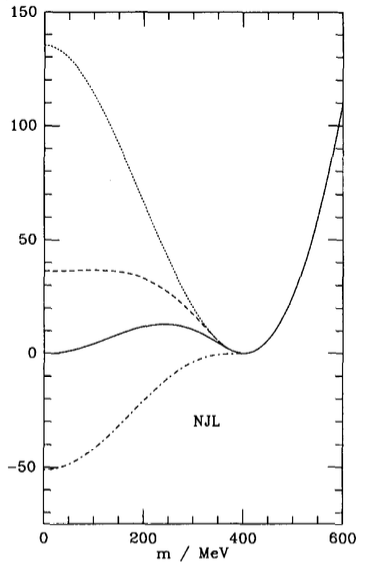
\includegraphics[width=0.45\textwidth]{graphics/Therm_pot_analysis/Pot_buballa.png}
	\caption{Gráfico do potencial termodinâmico $\tilde{\omega}$ obtido variando $m$ arbitrariamente, para o valor $\mu = 0$.}
	\label{Fig:pot_term_analysys_Buballa_NJL-Buballa_Set_1}
\end{figure*}

\begin{figure*}
	\begin{tikzpicture}[gnuplot]
%% generated with GNUPLOT 5.0p2 (Lua 5.2; terminal rev. 99, script rev. 100)
%% Wed Jun  1 15:20:44 2016
\path (0.000,0.000) rectangle (14.000,9.000);
\gpcolor{color=gp lt color border}
\gpsetlinetype{gp lt border}
\gpsetdashtype{gp dt solid}
\gpsetlinewidth{1.00}
\draw[gp path] (1.504,0.985)--(1.684,0.985);
\draw[gp path] (13.447,0.985)--(13.267,0.985);
\node[gp node right] at (1.320,0.985) {$1140$};
\draw[gp path] (1.504,2.259)--(1.684,2.259);
\draw[gp path] (13.447,2.259)--(13.267,2.259);
\node[gp node right] at (1.320,2.259) {$1160$};
\draw[gp path] (1.504,3.534)--(1.684,3.534);
\draw[gp path] (13.447,3.534)--(13.267,3.534);
\node[gp node right] at (1.320,3.534) {$1180$};
\draw[gp path] (1.504,4.808)--(1.684,4.808);
\draw[gp path] (13.447,4.808)--(13.267,4.808);
\node[gp node right] at (1.320,4.808) {$1200$};
\draw[gp path] (1.504,6.082)--(1.684,6.082);
\draw[gp path] (13.447,6.082)--(13.267,6.082);
\node[gp node right] at (1.320,6.082) {$1220$};
\draw[gp path] (1.504,7.357)--(1.684,7.357);
\draw[gp path] (13.447,7.357)--(13.267,7.357);
\node[gp node right] at (1.320,7.357) {$1240$};
\draw[gp path] (1.504,8.631)--(1.684,8.631);
\draw[gp path] (13.447,8.631)--(13.267,8.631);
\node[gp node right] at (1.320,8.631) {$1260$};
\draw[gp path] (1.504,0.985)--(1.504,1.165);
\draw[gp path] (1.504,8.631)--(1.504,8.451);
\node[gp node center] at (1.504,0.677) {$0$};
\draw[gp path] (3.495,0.985)--(3.495,1.165);
\draw[gp path] (3.495,8.631)--(3.495,8.451);
\node[gp node center] at (3.495,0.677) {$0.2$};
\draw[gp path] (5.485,0.985)--(5.485,1.165);
\draw[gp path] (5.485,8.631)--(5.485,8.451);
\node[gp node center] at (5.485,0.677) {$0.4$};
\draw[gp path] (7.476,0.985)--(7.476,1.165);
\draw[gp path] (7.476,8.631)--(7.476,8.451);
\node[gp node center] at (7.476,0.677) {$0.6$};
\draw[gp path] (9.466,0.985)--(9.466,1.165);
\draw[gp path] (9.466,8.631)--(9.466,8.451);
\node[gp node center] at (9.466,0.677) {$0.8$};
\draw[gp path] (11.456,0.985)--(11.456,1.165);
\draw[gp path] (11.456,8.631)--(11.456,8.451);
\node[gp node center] at (11.456,0.677) {$1$};
\draw[gp path] (13.447,0.985)--(13.447,1.165);
\draw[gp path] (13.447,8.631)--(13.447,8.451);
\node[gp node center] at (13.447,0.677) {$1.2$};
\draw[gp path] (1.504,8.631)--(1.504,0.985)--(13.447,0.985)--(13.447,8.631)--cycle;
\node[gp node center,rotate=-270] at (0.246,4.808) {$\varepsilon / \rho_B (\rm{MeV}$)};
\node[gp node center] at (7.475,0.215) {$\rho_B (\rm{MeV}/\rm{fm}^3)$};
\node[gp node right] at (11.979,8.297) {Fortran};
\gpcolor{rgb color={0.580,0.000,0.827}}
\gpsetlinewidth{4.00}
\draw[gp path] (12.163,8.297)--(13.079,8.297);
\draw[gp path] (12.432,8.185)--(12.382,8.121)--(12.332,8.058)--(12.283,7.994)--(12.223,7.930)%
  --(12.173,7.803)--(12.123,7.739)--(12.074,7.675)--(12.024,7.612)--(11.964,7.548)--(11.914,7.484)%
  --(11.865,7.357)--(11.815,7.293)--(11.765,7.229)--(11.715,7.166)--(11.666,7.102)--(11.616,7.038)%
  --(11.566,6.974)--(11.516,6.911)--(11.466,6.783)--(11.416,6.720)--(11.367,6.656)--(11.317,6.592)%
  --(11.268,6.528)--(11.220,6.465)--(11.171,6.401)--(11.122,6.337)--(11.074,6.273)--(11.027,6.210)%
  --(10.978,6.146)--(10.930,6.082)--(10.882,5.955)--(10.835,5.891)--(10.788,5.827)--(10.741,5.764)%
  --(10.693,5.700)--(10.646,5.636)--(10.600,5.573)--(10.553,5.509)--(10.507,5.445)--(10.460,5.381)%
  --(10.414,5.318)--(10.369,5.254)--(10.323,5.190)--(10.277,5.127)--(10.231,5.063)--(10.187,4.999)%
  --(10.141,4.935)--(10.096,4.872)--(10.051,4.808)--(10.006,4.808)--(9.962,4.744)--(9.917,4.681)%
  --(9.873,4.617)--(9.829,4.553)--(9.784,4.489)--(9.741,4.426)--(9.698,4.362)--(9.654,4.298)%
  --(9.610,4.235)--(9.568,4.171)--(9.525,4.107)--(9.481,4.107)--(9.438,4.043)--(9.396,3.980)%
  --(9.354,3.916)--(9.311,3.852)--(9.269,3.789)--(9.227,3.725)--(9.185,3.725)--(9.144,3.661)%
  --(9.102,3.597)--(9.060,3.534)--(9.019,3.470)--(8.977,3.470)--(8.937,3.406)--(8.896,3.343)%
  --(8.855,3.279)--(8.814,3.279)--(8.774,3.215)--(8.733,3.151)--(8.694,3.088)--(8.654,3.088)%
  --(8.614,3.024)--(8.574,2.960)--(8.534,2.897)--(8.495,2.897)--(8.456,2.833)--(8.416,2.769)%
  --(8.377,2.769)--(8.338,2.705)--(8.300,2.642)--(8.261,2.642)--(8.222,2.578)--(8.184,2.514)%
  --(8.145,2.514)--(8.107,2.450)--(8.070,2.450)--(8.032,2.387)--(7.994,2.323)--(7.956,2.323)%
  --(7.918,2.259)--(7.882,2.259)--(7.844,2.196)--(7.807,2.196)--(7.770,2.132)--(7.733,2.132)%
  --(7.696,2.068)--(7.660,2.068)--(7.624,2.004)--(7.587,2.004)--(7.551,1.941)--(7.514,1.941)%
  --(7.478,1.877)--(7.443,1.877)--(7.407,1.813)--(7.371,1.813)--(7.336,1.750)--(7.300,1.750)%
  --(7.265,1.750)--(7.230,1.686)--(7.195,1.686)--(7.159,1.686)--(7.124,1.622)--(7.089,1.622)%
  --(7.055,1.622)--(7.021,1.558)--(6.986,1.558)--(6.951,1.558)--(6.917,1.495)--(6.882,1.495)%
  --(6.848,1.495)--(6.815,1.495)--(6.780,1.495)--(6.746,1.431)--(6.712,1.431)--(6.678,1.431)%
  --(6.644,1.431)--(6.611,1.431)--(6.577,1.431)--(6.543,1.367)--(6.509,1.367)--(6.476,1.367)%
  --(6.442,1.367)--(6.409,1.367)--(6.375,1.367)--(6.341,1.367)--(6.307,1.367)--(6.273,1.367)%
  --(6.239,1.367)--(6.206,1.367)--(6.172,1.367)--(6.138,1.367)--(6.103,1.367)--(6.069,1.367)%
  --(6.034,1.431)--(6.000,1.431)--(5.964,1.431)--(5.928,1.431)--(5.892,1.431)--(5.855,1.495)%
  --(5.818,1.495)--(5.781,1.495)--(5.742,1.558)--(5.702,1.558)--(5.661,1.558)--(5.618,1.622)%
  --(5.574,1.622)--(5.527,1.686)--(5.476,1.750)--(5.420,1.813)--(5.356,1.877)--(5.277,1.941)%
  --(5.156,2.068)--(4.959,2.387);
\gpcolor{color=gp lt color border}
\node[gp node right] at (11.979,7.989) {C (Reimp. Fortran)};
\gpcolor{rgb color={0.000,0.620,0.451}}
\gpsetlinewidth{3.00}
\draw[gp path] (12.163,7.989)--(13.079,7.989);
\draw[gp path] (1.614,5.048)--(1.625,5.146)--(1.636,5.231)--(1.647,5.307)--(1.658,5.374)%
  --(1.669,5.434)--(1.680,5.489)--(1.690,5.539)--(1.701,5.585)--(1.712,5.626)--(1.723,5.665)%
  --(1.734,5.701)--(1.745,5.733)--(1.756,5.764)--(1.766,5.792)--(1.777,5.819)--(1.788,5.844)%
  --(1.799,5.867)--(1.810,5.888)--(1.821,5.908)--(1.832,5.927)--(1.842,5.944)--(1.853,5.960)%
  --(1.864,5.976)--(1.875,5.990)--(1.886,6.003)--(1.897,6.015)--(1.908,6.027)--(1.918,6.037)%
  --(1.929,6.047)--(1.940,6.056)--(1.951,6.064)--(1.962,6.072)--(1.973,6.079)--(1.984,6.085)%
  --(1.994,6.091)--(2.005,6.096)--(2.016,6.101)--(2.027,6.105)--(2.038,6.109)--(2.049,6.112)%
  --(2.060,6.115)--(2.070,6.117)--(2.081,6.119)--(2.092,6.120)--(2.103,6.121)--(2.114,6.121)%
  --(2.125,6.121)--(2.136,6.121)--(2.146,6.121)--(2.157,6.120)--(2.168,6.118)--(2.179,6.117)%
  --(2.190,6.115)--(2.201,6.113)--(2.212,6.110)--(2.222,6.107)--(2.233,6.104)--(2.244,6.100)%
  --(2.255,6.097)--(2.266,6.093)--(2.277,6.088)--(2.288,6.084)--(2.299,6.079)--(2.309,6.074)%
  --(2.320,6.069)--(2.331,6.063)--(2.342,6.058)--(2.353,6.052)--(2.364,6.046)--(2.375,6.039)%
  --(2.385,6.033)--(2.396,6.026)--(2.407,6.019)--(2.418,6.012)--(2.429,6.005)--(2.440,5.997)%
  --(2.451,5.989)--(2.461,5.981)--(2.472,5.973)--(2.483,5.965)--(2.494,5.957)--(2.505,5.948)%
  --(2.516,5.939)--(2.527,5.930)--(2.537,5.921)--(2.548,5.912)--(2.559,5.902)--(2.570,5.893)%
  --(2.581,5.883)--(2.592,5.873)--(2.603,5.863)--(2.613,5.853)--(2.624,5.843)--(2.635,5.833)%
  --(2.646,5.822)--(2.657,5.811)--(2.668,5.801)--(2.679,5.790)--(2.689,5.779)--(2.700,5.768)%
  --(2.711,5.756)--(2.722,5.745)--(2.733,5.733)--(2.744,5.722)--(2.755,5.710)--(2.765,5.698)%
  --(2.776,5.686)--(2.787,5.674)--(2.798,5.662)--(2.809,5.650)--(2.820,5.637)--(2.831,5.625)%
  --(2.841,5.612)--(2.852,5.599)--(2.863,5.587)--(2.874,5.574)--(2.885,5.561)--(2.896,5.548)%
  --(2.907,5.535)--(2.917,5.521)--(2.928,5.508)--(2.939,5.495)--(2.950,5.481)--(2.961,5.468)%
  --(2.972,5.454)--(2.983,5.440)--(2.993,5.426)--(3.004,5.412)--(3.015,5.398)--(3.026,5.384)%
  --(3.037,5.370)--(3.048,5.356)--(3.059,5.342)--(3.070,5.327)--(3.080,5.313)--(3.091,5.298)%
  --(3.102,5.284)--(3.113,5.269)--(3.124,5.254)--(3.135,5.239)--(3.146,5.224)--(3.156,5.210)%
  --(3.167,5.195)--(3.178,5.179)--(3.189,5.164)--(3.200,5.149)--(3.211,5.134)--(3.222,5.119)%
  --(3.232,5.103)--(3.243,5.088)--(3.254,5.072)--(3.265,5.057)--(3.276,5.041)--(3.287,5.025)%
  --(3.298,5.010)--(3.308,4.994)--(3.319,4.978)--(3.330,4.962)--(3.341,4.946)--(3.352,4.930)%
  --(3.363,4.914)--(3.374,4.898)--(3.384,4.882)--(3.395,4.866)--(3.406,4.850)--(3.417,4.833)%
  --(3.428,4.817)--(3.439,4.801)--(3.450,4.784)--(3.460,4.768)--(3.471,4.751)--(3.482,4.735)%
  --(3.493,4.718)--(3.504,4.702)--(3.515,4.685)--(3.526,4.668)--(3.536,4.652)--(3.547,4.635)%
  --(3.558,4.618)--(3.569,4.601)--(3.580,4.584)--(3.591,4.567)--(3.602,4.550)--(3.612,4.533)%
  --(3.623,4.516)--(3.634,4.499)--(3.645,4.482)--(3.656,4.465)--(3.667,4.448)--(3.678,4.431)%
  --(3.688,4.413)--(3.699,4.396)--(3.710,4.379)--(3.721,4.361)--(3.732,4.344)--(3.743,4.327)%
  --(3.754,4.309)--(3.764,4.292)--(3.775,4.274)--(3.786,4.257)--(3.797,4.239)--(3.808,4.222)%
  --(3.819,4.204)--(3.830,4.187)--(3.840,4.169)--(3.851,4.152)--(3.862,4.134)--(3.873,4.116)%
  --(3.884,4.099)--(3.895,4.081)--(3.906,4.063)--(3.917,4.045)--(3.927,4.028)--(3.938,4.010)%
  --(3.949,3.992)--(3.960,3.974)--(3.971,3.956)--(3.982,3.939)--(3.993,3.921)--(4.003,3.903)%
  --(4.014,3.885)--(4.025,3.867)--(4.036,3.849)--(4.047,3.831)--(4.058,3.813)--(4.069,3.795)%
  --(4.079,3.777)--(4.090,3.759)--(4.101,3.742)--(4.112,3.724)--(4.123,3.706)--(4.134,3.688)%
  --(4.145,3.670)--(4.155,3.652)--(4.166,3.634)--(4.177,3.616)--(4.188,3.598)--(4.199,3.580)%
  --(4.210,3.562)--(4.221,3.544)--(4.231,3.526)--(4.242,3.508)--(4.253,3.490)--(4.264,3.472)%
  --(4.275,3.454)--(4.286,3.436)--(4.297,3.418)--(4.307,3.400)--(4.318,3.382)--(4.329,3.364)%
  --(4.340,3.346)--(4.351,3.328)--(4.362,3.310)--(4.373,3.292)--(4.383,3.274)--(4.394,3.256)%
  --(4.405,3.238)--(4.416,3.221)--(4.427,3.203)--(4.438,3.185)--(4.449,3.167)--(4.459,3.149)%
  --(4.470,3.132)--(4.481,3.114)--(4.492,3.096)--(4.503,3.078)--(4.514,3.061)--(4.525,3.043)%
  --(4.535,3.025)--(4.546,3.008)--(4.557,2.990)--(4.568,2.973)--(4.579,2.955)--(4.590,2.937)%
  --(4.601,2.920)--(4.611,2.903)--(4.622,2.885)--(4.633,2.868)--(4.644,2.850)--(4.655,2.833)%
  --(4.666,2.816)--(4.677,2.799)--(4.688,2.782)--(4.698,2.764)--(4.709,2.747)--(4.720,2.730)%
  --(4.731,2.713)--(4.742,2.696)--(4.753,2.679)--(4.764,2.663)--(4.774,2.646)--(4.785,2.629)%
  --(4.796,2.612)--(4.807,2.596)--(4.818,2.579)--(4.829,2.563)--(4.840,2.546)--(4.850,2.530)%
  --(4.861,2.513)--(4.872,2.497)--(4.883,2.481)--(4.894,2.465)--(4.905,2.449)--(4.916,2.433)%
  --(4.926,2.417)--(4.937,2.401)--(4.948,2.385)--(4.959,2.370)--(4.970,2.354)--(4.981,2.338)%
  --(4.992,2.323)--(5.002,2.308)--(5.013,2.292)--(5.024,2.277)--(5.035,2.262)--(5.046,2.247)%
  --(5.057,2.232)--(5.068,2.217)--(5.078,2.203)--(5.089,2.188)--(5.100,2.173)--(5.111,2.159)%
  --(5.122,2.145)--(5.133,2.130)--(5.144,2.116)--(5.154,2.102)--(5.165,2.088)--(5.176,2.075)%
  --(5.187,2.061)--(5.198,2.047)--(5.209,2.034)--(5.220,2.021)--(5.230,2.008)--(5.241,1.994)%
  --(5.252,1.981)--(5.263,1.969)--(5.274,1.956)--(5.285,1.943)--(5.296,1.931)--(5.306,1.919)%
  --(5.317,1.906)--(5.328,1.894)--(5.339,1.882)--(5.350,1.870)--(5.361,1.859)--(5.372,1.847)%
  --(5.382,1.836)--(5.393,1.825)--(5.404,1.813)--(5.415,1.802)--(5.426,1.792)--(5.437,1.781)%
  --(5.448,1.770)--(5.458,1.760)--(5.469,1.749)--(5.480,1.739)--(5.491,1.729)--(5.502,1.719)%
  --(5.513,1.710)--(5.524,1.700)--(5.535,1.691)--(5.545,1.681)--(5.556,1.672)--(5.567,1.663)%
  --(5.578,1.654)--(5.589,1.645)--(5.600,1.637)--(5.611,1.628)--(5.621,1.620)--(5.632,1.612)%
  --(5.643,1.604)--(5.654,1.596)--(5.665,1.588)--(5.676,1.581)--(5.687,1.573)--(5.697,1.566)%
  --(5.708,1.559)--(5.719,1.552)--(5.730,1.545)--(5.741,1.538)--(5.752,1.532)--(5.763,1.525)%
  --(5.773,1.519)--(5.784,1.513)--(5.795,1.507)--(5.806,1.501)--(5.817,1.495)--(5.828,1.490)%
  --(5.839,1.484)--(5.849,1.479)--(5.860,1.474)--(5.871,1.469)--(5.882,1.464)--(5.893,1.459)%
  --(5.904,1.454)--(5.915,1.450)--(5.925,1.446)--(5.936,1.441)--(5.947,1.437)--(5.958,1.433)%
  --(5.969,1.429)--(5.980,1.426)--(5.991,1.422)--(6.001,1.419)--(6.012,1.416)--(6.023,1.412)%
  --(6.034,1.409)--(6.045,1.406)--(6.056,1.404)--(6.067,1.401)--(6.077,1.399)--(6.088,1.396)%
  --(6.099,1.394)--(6.110,1.392)--(6.121,1.390)--(6.132,1.388)--(6.143,1.386)--(6.153,1.384)%
  --(6.164,1.383)--(6.175,1.381)--(6.186,1.380)--(6.197,1.379)--(6.208,1.378)--(6.219,1.377)%
  --(6.229,1.376)--(6.240,1.376)--(6.251,1.375)--(6.262,1.375)--(6.273,1.374)--(6.284,1.374)%
  --(6.295,1.374)--(6.306,1.374)--(6.316,1.374)--(6.327,1.374)--(6.338,1.374)--(6.349,1.375)%
  --(6.360,1.375)--(6.371,1.376)--(6.382,1.377)--(6.392,1.378)--(6.403,1.379)--(6.414,1.380)%
  --(6.425,1.381)--(6.436,1.382)--(6.447,1.383)--(6.458,1.385)--(6.468,1.387)--(6.479,1.388)%
  --(6.490,1.390)--(6.501,1.392)--(6.512,1.394)--(6.523,1.396)--(6.534,1.398)--(6.544,1.400)%
  --(6.555,1.403)--(6.566,1.405)--(6.577,1.408)--(6.588,1.410)--(6.599,1.413)--(6.610,1.416)%
  --(6.620,1.419)--(6.631,1.422)--(6.642,1.425)--(6.653,1.428)--(6.664,1.432)--(6.675,1.435)%
  --(6.686,1.438)--(6.696,1.442)--(6.707,1.446)--(6.718,1.449)--(6.729,1.453)--(6.740,1.457)%
  --(6.751,1.461)--(6.762,1.465)--(6.772,1.469)--(6.783,1.474)--(6.794,1.478)--(6.805,1.482)%
  --(6.816,1.487)--(6.827,1.491)--(6.838,1.496)--(6.848,1.501)--(6.859,1.506)--(6.870,1.511)%
  --(6.881,1.516)--(6.892,1.521)--(6.903,1.526)--(6.914,1.531)--(6.924,1.536)--(6.935,1.542)%
  --(6.946,1.547)--(6.957,1.553)--(6.968,1.558)--(6.979,1.564)--(6.990,1.570)--(7.000,1.575)%
  --(7.011,1.581)--(7.022,1.587)--(7.033,1.593)--(7.044,1.599)--(7.055,1.605)--(7.066,1.612)%
  --(7.077,1.618)--(7.087,1.624)--(7.098,1.631)--(7.109,1.637)--(7.120,1.644)--(7.131,1.650)%
  --(7.142,1.657)--(7.153,1.664)--(7.163,1.671)--(7.174,1.678)--(7.185,1.685)--(7.196,1.692)%
  --(7.207,1.699)--(7.218,1.706)--(7.229,1.713)--(7.239,1.720)--(7.250,1.728)--(7.261,1.735)%
  --(7.272,1.743)--(7.283,1.750)--(7.294,1.758)--(7.305,1.765)--(7.315,1.773)--(7.326,1.781)%
  --(7.337,1.789)--(7.348,1.796)--(7.359,1.804)--(7.370,1.812)--(7.381,1.820)--(7.391,1.829)%
  --(7.402,1.837)--(7.413,1.845)--(7.424,1.853)--(7.435,1.862)--(7.446,1.870)--(7.457,1.878)%
  --(7.467,1.887)--(7.478,1.895)--(7.489,1.904)--(7.500,1.913)--(7.511,1.921)--(7.522,1.930)%
  --(7.533,1.939)--(7.543,1.948)--(7.554,1.957)--(7.565,1.966)--(7.576,1.975)--(7.587,1.984)%
  --(7.598,1.993)--(7.609,2.002)--(7.619,2.011)--(7.630,2.020)--(7.641,2.030)--(7.652,2.039)%
  --(7.663,2.048)--(7.674,2.058)--(7.685,2.067)--(7.695,2.077)--(7.706,2.086)--(7.717,2.096)%
  --(7.728,2.106)--(7.739,2.115)--(7.750,2.125)--(7.761,2.135)--(7.771,2.145)--(7.782,2.155)%
  --(7.793,2.165)--(7.804,2.175)--(7.815,2.185)--(7.826,2.195)--(7.837,2.205)--(7.847,2.215)%
  --(7.858,2.225)--(7.869,2.235)--(7.880,2.246)--(7.891,2.256)--(7.902,2.266)--(7.913,2.277)%
  --(7.924,2.287)--(7.934,2.298)--(7.945,2.308)--(7.956,2.319)--(7.967,2.329)--(7.978,2.340)%
  --(7.989,2.351)--(8.000,2.361)--(8.010,2.372)--(8.021,2.383)--(8.032,2.394)--(8.043,2.405)%
  --(8.054,2.415)--(8.065,2.426)--(8.076,2.437)--(8.086,2.448)--(8.097,2.459)--(8.108,2.471)%
  --(8.119,2.482)--(8.130,2.493)--(8.141,2.504)--(8.152,2.515)--(8.162,2.526)--(8.173,2.538)%
  --(8.184,2.549)--(8.195,2.560)--(8.206,2.572)--(8.217,2.583)--(8.228,2.595)--(8.238,2.606)%
  --(8.249,2.618)--(8.260,2.629)--(8.271,2.641)--(8.282,2.652)--(8.293,2.664)--(8.304,2.676)%
  --(8.314,2.687)--(8.325,2.699)--(8.336,2.711)--(8.347,2.723)--(8.358,2.735)--(8.369,2.746)%
  --(8.380,2.758)--(8.390,2.770)--(8.401,2.782)--(8.412,2.794)--(8.423,2.806)--(8.434,2.818)%
  --(8.445,2.830)--(8.456,2.842)--(8.466,2.855)--(8.477,2.867)--(8.488,2.879)--(8.499,2.891)%
  --(8.510,2.903)--(8.521,2.916)--(8.532,2.928)--(8.542,2.940)--(8.553,2.953)--(8.564,2.965)%
  --(8.575,2.977)--(8.586,2.990)--(8.597,3.002)--(8.608,3.015)--(8.618,3.027)--(8.629,3.040)%
  --(8.640,3.052)--(8.651,3.065)--(8.662,3.077)--(8.673,3.090)--(8.684,3.103)--(8.695,3.115)%
  --(8.705,3.128)--(8.716,3.141)--(8.727,3.154)--(8.738,3.166)--(8.749,3.179)--(8.760,3.192)%
  --(8.771,3.205)--(8.781,3.218)--(8.792,3.231)--(8.803,3.243)--(8.814,3.256)--(8.825,3.269)%
  --(8.836,3.282)--(8.847,3.295)--(8.857,3.308)--(8.868,3.321)--(8.879,3.334)--(8.890,3.348)%
  --(8.901,3.361)--(8.912,3.374)--(8.923,3.387)--(8.933,3.400)--(8.944,3.413)--(8.955,3.427)%
  --(8.966,3.440)--(8.977,3.453)--(8.988,3.466)--(8.999,3.480)--(9.009,3.493)--(9.020,3.506)%
  --(9.031,3.520)--(9.042,3.533)--(9.053,3.546)--(9.064,3.560)--(9.075,3.573)--(9.085,3.587)%
  --(9.096,3.600)--(9.107,3.614)--(9.118,3.627)--(9.129,3.641)--(9.140,3.654)--(9.151,3.668)%
  --(9.161,3.681)--(9.172,3.695)--(9.183,3.709)--(9.194,3.722)--(9.205,3.736)--(9.216,3.750)%
  --(9.227,3.763)--(9.237,3.777)--(9.248,3.791)--(9.259,3.804)--(9.270,3.818)--(9.281,3.832)%
  --(9.292,3.846)--(9.303,3.860)--(9.313,3.873)--(9.324,3.887)--(9.335,3.901)--(9.346,3.915)%
  --(9.357,3.929)--(9.368,3.943)--(9.379,3.957)--(9.389,3.971)--(9.400,3.985)--(9.411,3.999)%
  --(9.422,4.013)--(9.433,4.027)--(9.444,4.041)--(9.455,4.055)--(9.466,4.069)--(9.476,4.083)%
  --(9.487,4.097)--(9.498,4.111)--(9.509,4.125)--(9.520,4.139)--(9.531,4.153)--(9.542,4.167)%
  --(9.552,4.181)--(9.563,4.196)--(9.574,4.210)--(9.585,4.224)--(9.596,4.238)--(9.607,4.252)%
  --(9.618,4.267)--(9.628,4.281)--(9.639,4.295)--(9.650,4.309)--(9.661,4.324)--(9.672,4.338)%
  --(9.683,4.352)--(9.694,4.367)--(9.704,4.381)--(9.715,4.395)--(9.726,4.410)--(9.737,4.424)%
  --(9.748,4.439)--(9.759,4.453)--(9.770,4.467)--(9.780,4.482)--(9.791,4.496)--(9.802,4.511)%
  --(9.813,4.525)--(9.824,4.540)--(9.835,4.554)--(9.846,4.569)--(9.856,4.583)--(9.867,4.598)%
  --(9.878,4.612)--(9.889,4.627)--(9.900,4.641)--(9.911,4.656)--(9.922,4.670)--(9.932,4.685)%
  --(9.943,4.700)--(9.954,4.714)--(9.965,4.729)--(9.976,4.743)--(9.987,4.758)--(9.998,4.773)%
  --(10.008,4.787)--(10.019,4.802)--(10.030,4.817)--(10.041,4.831)--(10.052,4.846)--(10.063,4.861)%
  --(10.074,4.876)--(10.084,4.890)--(10.095,4.905)--(10.106,4.920)--(10.117,4.935)--(10.128,4.949)%
  --(10.139,4.964)--(10.150,4.979)--(10.160,4.994)--(10.171,5.008)--(10.182,5.023)--(10.193,5.038)%
  --(10.204,5.053)--(10.215,5.068)--(10.226,5.083)--(10.236,5.097)--(10.247,5.112)--(10.258,5.127)%
  --(10.269,5.142)--(10.280,5.157)--(10.291,5.172)--(10.302,5.187)--(10.313,5.202)--(10.323,5.217)%
  --(10.334,5.232)--(10.345,5.246)--(10.356,5.261)--(10.367,5.276)--(10.378,5.291)--(10.389,5.306)%
  --(10.399,5.321)--(10.410,5.336)--(10.421,5.351)--(10.432,5.366)--(10.443,5.381)--(10.454,5.396)%
  --(10.465,5.411)--(10.475,5.426)--(10.486,5.441)--(10.497,5.456)--(10.508,5.471)--(10.519,5.487)%
  --(10.530,5.502)--(10.541,5.517)--(10.551,5.532)--(10.562,5.547)--(10.573,5.562)--(10.584,5.577)%
  --(10.595,5.592)--(10.606,5.607)--(10.617,5.622)--(10.627,5.637)--(10.638,5.653)--(10.649,5.668)%
  --(10.660,5.683)--(10.671,5.698)--(10.682,5.713)--(10.693,5.728)--(10.703,5.744)--(10.714,5.759)%
  --(10.725,5.774)--(10.736,5.789)--(10.747,5.804)--(10.758,5.819)--(10.769,5.835)--(10.779,5.850)%
  --(10.790,5.865)--(10.801,5.880)--(10.812,5.896)--(10.823,5.911)--(10.834,5.926)--(10.845,5.941)%
  --(10.855,5.956)--(10.866,5.972)--(10.877,5.987)--(10.888,6.002)--(10.899,6.018)--(10.910,6.033)%
  --(10.921,6.048)--(10.931,6.063)--(10.942,6.079)--(10.953,6.094)--(10.964,6.109)--(10.975,6.125)%
  --(10.986,6.140)--(10.997,6.155)--(11.007,6.170)--(11.018,6.186)--(11.029,6.201)--(11.040,6.216)%
  --(11.051,6.232)--(11.062,6.247)--(11.073,6.262)--(11.084,6.278)--(11.094,6.293)--(11.105,6.308)%
  --(11.116,6.324)--(11.127,6.339)--(11.138,6.355)--(11.149,6.370)--(11.160,6.385)--(11.170,6.401)%
  --(11.181,6.416)--(11.192,6.431)--(11.203,6.447)--(11.214,6.462)--(11.225,6.478)--(11.236,6.493)%
  --(11.246,6.508)--(11.257,6.524)--(11.268,6.539)--(11.279,6.555)--(11.290,6.570)--(11.301,6.586)%
  --(11.312,6.601)--(11.322,6.616)--(11.333,6.632)--(11.344,6.647)--(11.355,6.663)--(11.366,6.678)%
  --(11.377,6.694)--(11.388,6.709)--(11.398,6.725)--(11.409,6.740)--(11.420,6.755)--(11.431,6.771)%
  --(11.442,6.786)--(11.453,6.802)--(11.464,6.817)--(11.474,6.833)--(11.485,6.848)--(11.496,6.864)%
  --(11.507,6.879)--(11.518,6.895)--(11.529,6.910)--(11.540,6.926)--(11.550,6.941)--(11.561,6.957)%
  --(11.572,6.972)--(11.583,6.988)--(11.594,7.003)--(11.605,7.019)--(11.616,7.034)--(11.626,7.050)%
  --(11.637,7.065)--(11.648,7.081)--(11.659,7.096)--(11.670,7.112)--(11.681,7.127)--(11.692,7.143)%
  --(11.702,7.158)--(11.713,7.174)--(11.724,7.189)--(11.735,7.205)--(11.746,7.220)--(11.757,7.236)%
  --(11.768,7.252)--(11.778,7.267)--(11.789,7.283)--(11.800,7.298)--(11.811,7.314)--(11.822,7.329)%
  --(11.833,7.345)--(11.844,7.360)--(11.855,7.376)--(11.865,7.392)--(11.876,7.407)--(11.887,7.423)%
  --(11.898,7.438)--(11.909,7.454)--(11.920,7.469)--(11.931,7.485)--(11.941,7.500)--(11.952,7.516)%
  --(11.963,7.532)--(11.974,7.547)--(11.985,7.563)--(11.996,7.578)--(12.007,7.594)--(12.017,7.609)%
  --(12.028,7.625)--(12.039,7.641)--(12.050,7.656)--(12.061,7.672)--(12.072,7.687)--(12.083,7.703)%
  --(12.093,7.719)--(12.104,7.734)--(12.115,7.750)--(12.126,7.765)--(12.137,7.781)--(12.148,7.797)%
  --(12.159,7.812)--(12.169,7.828)--(12.180,7.843)--(12.191,7.859)--(12.202,7.874)--(12.213,7.890)%
  --(12.224,7.906)--(12.235,7.921)--(12.245,7.937)--(12.256,7.952)--(12.267,7.968)--(12.278,7.984)%
  --(12.289,7.999)--(12.300,8.015)--(12.311,8.030)--(12.321,8.046)--(12.332,8.062)--(12.343,8.077)%
  --(12.354,8.093)--(12.365,8.109)--(12.376,8.124)--(12.387,8.140)--(12.397,8.155)--(12.408,8.171)%
  --(12.419,8.187)--(12.430,8.202)--(12.441,8.218)--(12.452,8.233)--(12.463,8.249);
\gpcolor{color=gp lt color border}
\node[gp node right] at (11.979,7.681) {C (Buballa)};
\gpcolor{rgb color={0.337,0.706,0.914}}
\gpsetlinewidth{2.00}
\draw[gp path] (12.163,7.681)--(13.079,7.681);
\draw[gp path] (1.614,5.048)--(1.625,5.146)--(1.636,5.231)--(1.647,5.307)--(1.658,5.374)%
  --(1.669,5.434)--(1.680,5.489)--(1.690,5.539)--(1.701,5.585)--(1.712,5.626)--(1.723,5.665)%
  --(1.734,5.701)--(1.745,5.733)--(1.756,5.764)--(1.766,5.792)--(1.777,5.819)--(1.788,5.844)%
  --(1.799,5.867)--(1.810,5.888)--(1.821,5.908)--(1.832,5.927)--(1.842,5.944)--(1.853,5.960)%
  --(1.864,5.976)--(1.875,5.990)--(1.886,6.003)--(1.897,6.015)--(1.908,6.027)--(1.918,6.037)%
  --(1.929,6.047)--(1.940,6.056)--(1.951,6.064)--(1.962,6.072)--(1.973,6.079)--(1.984,6.085)%
  --(1.994,6.091)--(2.005,6.096)--(2.016,6.101)--(2.027,6.105)--(2.038,6.109)--(2.049,6.112)%
  --(2.060,6.115)--(2.070,6.117)--(2.081,6.119)--(2.092,6.120)--(2.103,6.121)--(2.114,6.121)%
  --(2.125,6.121)--(2.136,6.121)--(2.146,6.121)--(2.157,6.120)--(2.168,6.118)--(2.179,6.117)%
  --(2.190,6.115)--(2.201,6.113)--(2.212,6.110)--(2.222,6.107)--(2.233,6.104)--(2.244,6.100)%
  --(2.255,6.097)--(2.266,6.093)--(2.277,6.088)--(2.288,6.084)--(2.299,6.079)--(2.309,6.074)%
  --(2.320,6.069)--(2.331,6.063)--(2.342,6.058)--(2.353,6.052)--(2.364,6.046)--(2.375,6.039)%
  --(2.385,6.033)--(2.396,6.026)--(2.407,6.019)--(2.418,6.012)--(2.429,6.005)--(2.440,5.997)%
  --(2.451,5.989)--(2.461,5.981)--(2.472,5.973)--(2.483,5.965)--(2.494,5.957)--(2.505,5.948)%
  --(2.516,5.939)--(2.527,5.930)--(2.537,5.921)--(2.548,5.912)--(2.559,5.902)--(2.570,5.893)%
  --(2.581,5.883)--(2.592,5.873)--(2.603,5.863)--(2.613,5.853)--(2.624,5.843)--(2.635,5.833)%
  --(2.646,5.822)--(2.657,5.811)--(2.668,5.801)--(2.679,5.790)--(2.689,5.779)--(2.700,5.768)%
  --(2.711,5.756)--(2.722,5.745)--(2.733,5.733)--(2.744,5.722)--(2.755,5.710)--(2.765,5.698)%
  --(2.776,5.686)--(2.787,5.674)--(2.798,5.662)--(2.809,5.650)--(2.820,5.637)--(2.831,5.625)%
  --(2.841,5.612)--(2.852,5.599)--(2.863,5.587)--(2.874,5.574)--(2.885,5.561)--(2.896,5.548)%
  --(2.907,5.535)--(2.917,5.521)--(2.928,5.508)--(2.939,5.495)--(2.950,5.481)--(2.961,5.468)%
  --(2.972,5.454)--(2.983,5.440)--(2.993,5.426)--(3.004,5.412)--(3.015,5.398)--(3.026,5.384)%
  --(3.037,5.370)--(3.048,5.356)--(3.059,5.342)--(3.070,5.327)--(3.080,5.313)--(3.091,5.298)%
  --(3.102,5.284)--(3.113,5.269)--(3.124,5.254)--(3.135,5.239)--(3.146,5.224)--(3.156,5.210)%
  --(3.167,5.195)--(3.178,5.179)--(3.189,5.164)--(3.200,5.149)--(3.211,5.134)--(3.222,5.119)%
  --(3.232,5.103)--(3.243,5.088)--(3.254,5.072)--(3.265,5.057)--(3.276,5.041)--(3.287,5.025)%
  --(3.298,5.010)--(3.308,4.994)--(3.319,4.978)--(3.330,4.962)--(3.341,4.946)--(3.352,4.930)%
  --(3.363,4.914)--(3.374,4.898)--(3.384,4.882)--(3.395,4.866)--(3.406,4.850)--(3.417,4.833)%
  --(3.428,4.817)--(3.439,4.801)--(3.450,4.784)--(3.460,4.768)--(3.471,4.751)--(3.482,4.735)%
  --(3.493,4.718)--(3.504,4.702)--(3.515,4.685)--(3.526,4.668)--(3.536,4.652)--(3.547,4.635)%
  --(3.558,4.618)--(3.569,4.601)--(3.580,4.584)--(3.591,4.567)--(3.602,4.550)--(3.612,4.533)%
  --(3.623,4.516)--(3.634,4.499)--(3.645,4.482)--(3.656,4.465)--(3.667,4.448)--(3.678,4.431)%
  --(3.688,4.413)--(3.699,4.396)--(3.710,4.379)--(3.721,4.361)--(3.732,4.344)--(3.743,4.327)%
  --(3.754,4.309)--(3.764,4.292)--(3.775,4.274)--(3.786,4.257)--(3.797,4.239)--(3.808,4.222)%
  --(3.819,4.204)--(3.830,4.187)--(3.840,4.169)--(3.851,4.152)--(3.862,4.134)--(3.873,4.116)%
  --(3.884,4.099)--(3.895,4.081)--(3.906,4.063)--(3.917,4.045)--(3.927,4.028)--(3.938,4.010)%
  --(3.949,3.992)--(3.960,3.974)--(3.971,3.956)--(3.982,3.939)--(3.993,3.921)--(4.003,3.903)%
  --(4.014,3.885)--(4.025,3.867)--(4.036,3.849)--(4.047,3.831)--(4.058,3.813)--(4.069,3.795)%
  --(4.079,3.777)--(4.090,3.759)--(4.101,3.742)--(4.112,3.724)--(4.123,3.706)--(4.134,3.688)%
  --(4.145,3.670)--(4.155,3.652)--(4.166,3.634)--(4.177,3.616)--(4.188,3.598)--(4.199,3.580)%
  --(4.210,3.562)--(4.221,3.544)--(4.231,3.526)--(4.242,3.508)--(4.253,3.490)--(4.264,3.472)%
  --(4.275,3.454)--(4.286,3.436)--(4.297,3.418)--(4.307,3.400)--(4.318,3.382)--(4.329,3.364)%
  --(4.340,3.346)--(4.351,3.328)--(4.362,3.310)--(4.373,3.292)--(4.383,3.274)--(4.394,3.256)%
  --(4.405,3.238)--(4.416,3.221)--(4.427,3.203)--(4.438,3.185)--(4.449,3.167)--(4.459,3.149)%
  --(4.470,3.132)--(4.481,3.114)--(4.492,3.096)--(4.503,3.078)--(4.514,3.061)--(4.525,3.043)%
  --(4.535,3.025)--(4.546,3.008)--(4.557,2.990)--(4.568,2.973)--(4.579,2.955)--(4.590,2.937)%
  --(4.601,2.920)--(4.611,2.903)--(4.622,2.885)--(4.633,2.868)--(4.644,2.850)--(4.655,2.833)%
  --(4.666,2.816)--(4.677,2.799)--(4.688,2.782)--(4.698,2.764)--(4.709,2.747)--(4.720,2.730)%
  --(4.731,2.713)--(4.742,2.696)--(4.753,2.679)--(4.764,2.663)--(4.774,2.646)--(4.785,2.629)%
  --(4.796,2.612)--(4.807,2.596)--(4.818,2.579)--(4.829,2.563)--(4.840,2.546)--(4.850,2.530)%
  --(4.861,2.513)--(4.872,2.497)--(4.883,2.481)--(4.894,2.465)--(4.905,2.449)--(4.916,2.433)%
  --(4.926,2.417)--(4.937,2.401)--(4.948,2.385)--(4.959,2.370)--(4.970,2.354)--(4.981,2.338)%
  --(4.992,2.323)--(5.002,2.308)--(5.013,2.292)--(5.024,2.277)--(5.035,2.262)--(5.046,2.247)%
  --(5.057,2.232)--(5.068,2.217)--(5.078,2.203)--(5.089,2.188)--(5.100,2.173)--(5.111,2.159)%
  --(5.122,2.145)--(5.133,2.130)--(5.144,2.116)--(5.154,2.102)--(5.165,2.088)--(5.176,2.075)%
  --(5.187,2.061)--(5.198,2.047)--(5.209,2.034)--(5.220,2.021)--(5.230,2.008)--(5.241,1.994)%
  --(5.252,1.981)--(5.263,1.969)--(5.274,1.956)--(5.285,1.943)--(5.296,1.931)--(5.306,1.919)%
  --(5.317,1.906)--(5.328,1.894)--(5.339,1.882)--(5.350,1.870)--(5.361,1.859)--(5.372,1.847)%
  --(5.382,1.836)--(5.393,1.825)--(5.404,1.813)--(5.415,1.802)--(5.426,1.792)--(5.437,1.781)%
  --(5.448,1.770)--(5.458,1.760)--(5.469,1.749)--(5.480,1.739)--(5.491,1.729)--(5.502,1.719)%
  --(5.513,1.710)--(5.524,1.700)--(5.535,1.691)--(5.545,1.681)--(5.556,1.672)--(5.567,1.663)%
  --(5.578,1.654)--(5.589,1.645)--(5.600,1.637)--(5.611,1.628)--(5.621,1.620)--(5.632,1.612)%
  --(5.643,1.604)--(5.654,1.596)--(5.665,1.588)--(5.676,1.581)--(5.687,1.573)--(5.697,1.566)%
  --(5.708,1.559)--(5.719,1.552)--(5.730,1.545)--(5.741,1.538)--(5.752,1.532)--(5.763,1.525)%
  --(5.773,1.519)--(5.784,1.513)--(5.795,1.507)--(5.806,1.501)--(5.817,1.495)--(5.828,1.490)%
  --(5.839,1.484)--(5.849,1.479)--(5.860,1.474)--(5.871,1.469)--(5.882,1.464)--(5.893,1.459)%
  --(5.904,1.454)--(5.915,1.450)--(5.925,1.446)--(5.936,1.441)--(5.947,1.437)--(5.958,1.433)%
  --(5.969,1.429)--(5.980,1.426)--(5.991,1.422)--(6.001,1.419)--(6.012,1.416)--(6.023,1.412)%
  --(6.034,1.409)--(6.045,1.406)--(6.056,1.404)--(6.067,1.401)--(6.077,1.399)--(6.088,1.396)%
  --(6.099,1.394)--(6.110,1.392)--(6.121,1.390)--(6.132,1.388)--(6.143,1.386)--(6.153,1.384)%
  --(6.164,1.383)--(6.175,1.381)--(6.186,1.380)--(6.197,1.379)--(6.208,1.378)--(6.219,1.377)%
  --(6.229,1.376)--(6.240,1.376)--(6.251,1.375)--(6.262,1.375)--(6.273,1.374)--(6.284,1.374)%
  --(6.295,1.374)--(6.306,1.374)--(6.316,1.374)--(6.327,1.374)--(6.338,1.374)--(6.349,1.375)%
  --(6.360,1.375)--(6.371,1.376)--(6.382,1.377)--(6.392,1.378)--(6.403,1.379)--(6.414,1.380)%
  --(6.425,1.381)--(6.436,1.382)--(6.447,1.383)--(6.458,1.385)--(6.468,1.387)--(6.479,1.388)%
  --(6.490,1.390)--(6.501,1.392)--(6.512,1.394)--(6.523,1.396)--(6.534,1.398)--(6.544,1.400)%
  --(6.555,1.403)--(6.566,1.405)--(6.577,1.408)--(6.588,1.410)--(6.599,1.413)--(6.610,1.416)%
  --(6.620,1.419)--(6.631,1.422)--(6.642,1.425)--(6.653,1.428)--(6.664,1.432)--(6.675,1.435)%
  --(6.686,1.438)--(6.696,1.442)--(6.707,1.446)--(6.718,1.449)--(6.729,1.453)--(6.740,1.457)%
  --(6.751,1.461)--(6.762,1.465)--(6.772,1.469)--(6.783,1.474)--(6.794,1.478)--(6.805,1.482)%
  --(6.816,1.487)--(6.827,1.491)--(6.838,1.496)--(6.848,1.501)--(6.859,1.506)--(6.870,1.511)%
  --(6.881,1.516)--(6.892,1.521)--(6.903,1.526)--(6.914,1.531)--(6.924,1.536)--(6.935,1.542)%
  --(6.946,1.547)--(6.957,1.553)--(6.968,1.558)--(6.979,1.564)--(6.990,1.570)--(7.000,1.575)%
  --(7.011,1.581)--(7.022,1.587)--(7.033,1.593)--(7.044,1.599)--(7.055,1.605)--(7.066,1.612)%
  --(7.077,1.618)--(7.087,1.624)--(7.098,1.631)--(7.109,1.637)--(7.120,1.644)--(7.131,1.650)%
  --(7.142,1.657)--(7.153,1.664)--(7.163,1.671)--(7.174,1.678)--(7.185,1.685)--(7.196,1.692)%
  --(7.207,1.699)--(7.218,1.706)--(7.229,1.713)--(7.239,1.720)--(7.250,1.728)--(7.261,1.735)%
  --(7.272,1.743)--(7.283,1.750)--(7.294,1.758)--(7.305,1.765)--(7.315,1.773)--(7.326,1.781)%
  --(7.337,1.789)--(7.348,1.796)--(7.359,1.804)--(7.370,1.812)--(7.381,1.820)--(7.391,1.829)%
  --(7.402,1.837)--(7.413,1.845)--(7.424,1.853)--(7.435,1.862)--(7.446,1.870)--(7.457,1.878)%
  --(7.467,1.887)--(7.478,1.895)--(7.489,1.904)--(7.500,1.913)--(7.511,1.921)--(7.522,1.930)%
  --(7.533,1.939)--(7.543,1.948)--(7.554,1.957)--(7.565,1.966)--(7.576,1.975)--(7.587,1.984)%
  --(7.598,1.993)--(7.609,2.002)--(7.619,2.011)--(7.630,2.020)--(7.641,2.030)--(7.652,2.039)%
  --(7.663,2.048)--(7.674,2.058)--(7.685,2.067)--(7.695,2.077)--(7.706,2.086)--(7.717,2.096)%
  --(7.728,2.106)--(7.739,2.115)--(7.750,2.125)--(7.761,2.135)--(7.771,2.145)--(7.782,2.155)%
  --(7.793,2.165)--(7.804,2.175)--(7.815,2.185)--(7.826,2.195)--(7.837,2.205)--(7.847,2.215)%
  --(7.858,2.225)--(7.869,2.235)--(7.880,2.246)--(7.891,2.256)--(7.902,2.266)--(7.913,2.277)%
  --(7.924,2.287)--(7.934,2.298)--(7.945,2.308)--(7.956,2.319)--(7.967,2.329)--(7.978,2.340)%
  --(7.989,2.351)--(8.000,2.361)--(8.010,2.372)--(8.021,2.383)--(8.032,2.394)--(8.043,2.405)%
  --(8.054,2.415)--(8.065,2.426)--(8.076,2.437)--(8.086,2.448)--(8.097,2.459)--(8.108,2.471)%
  --(8.119,2.482)--(8.130,2.493)--(8.141,2.504)--(8.152,2.515)--(8.162,2.526)--(8.173,2.538)%
  --(8.184,2.549)--(8.195,2.560)--(8.206,2.572)--(8.217,2.583)--(8.228,2.595)--(8.238,2.606)%
  --(8.249,2.618)--(8.260,2.629)--(8.271,2.641)--(8.282,2.652)--(8.293,2.664)--(8.304,2.676)%
  --(8.314,2.687)--(8.325,2.699)--(8.336,2.711)--(8.347,2.723)--(8.358,2.735)--(8.369,2.746)%
  --(8.380,2.758)--(8.390,2.770)--(8.401,2.782)--(8.412,2.794)--(8.423,2.806)--(8.434,2.818)%
  --(8.445,2.830)--(8.456,2.842)--(8.466,2.855)--(8.477,2.867)--(8.488,2.879)--(8.499,2.891)%
  --(8.510,2.903)--(8.521,2.916)--(8.532,2.928)--(8.542,2.940)--(8.553,2.953)--(8.564,2.965)%
  --(8.575,2.977)--(8.586,2.990)--(8.597,3.002)--(8.608,3.015)--(8.618,3.027)--(8.629,3.040)%
  --(8.640,3.052)--(8.651,3.065)--(8.662,3.077)--(8.673,3.090)--(8.684,3.103)--(8.695,3.115)%
  --(8.705,3.128)--(8.716,3.141)--(8.727,3.154)--(8.738,3.166)--(8.749,3.179)--(8.760,3.192)%
  --(8.771,3.205)--(8.781,3.218)--(8.792,3.231)--(8.803,3.243)--(8.814,3.256)--(8.825,3.269)%
  --(8.836,3.282)--(8.847,3.295)--(8.857,3.308)--(8.868,3.321)--(8.879,3.334)--(8.890,3.348)%
  --(8.901,3.361)--(8.912,3.374)--(8.923,3.387)--(8.933,3.400)--(8.944,3.413)--(8.955,3.427)%
  --(8.966,3.440)--(8.977,3.453)--(8.988,3.466)--(8.999,3.480)--(9.009,3.493)--(9.020,3.506)%
  --(9.031,3.520)--(9.042,3.533)--(9.053,3.546)--(9.064,3.560)--(9.075,3.573)--(9.085,3.587)%
  --(9.096,3.600)--(9.107,3.614)--(9.118,3.627)--(9.129,3.641)--(9.140,3.654)--(9.151,3.668)%
  --(9.161,3.681)--(9.172,3.695)--(9.183,3.709)--(9.194,3.722)--(9.205,3.736)--(9.216,3.750)%
  --(9.227,3.763)--(9.237,3.777)--(9.248,3.791)--(9.259,3.804)--(9.270,3.818)--(9.281,3.832)%
  --(9.292,3.846)--(9.303,3.860)--(9.313,3.873)--(9.324,3.887)--(9.335,3.901)--(9.346,3.915)%
  --(9.357,3.929)--(9.368,3.943)--(9.379,3.957)--(9.389,3.971)--(9.400,3.985)--(9.411,3.999)%
  --(9.422,4.013)--(9.433,4.027)--(9.444,4.041)--(9.455,4.055)--(9.466,4.069)--(9.476,4.083)%
  --(9.487,4.097)--(9.498,4.111)--(9.509,4.125)--(9.520,4.139)--(9.531,4.153)--(9.542,4.167)%
  --(9.552,4.181)--(9.563,4.196)--(9.574,4.210)--(9.585,4.224)--(9.596,4.238)--(9.607,4.252)%
  --(9.618,4.267)--(9.628,4.281)--(9.639,4.295)--(9.650,4.309)--(9.661,4.324)--(9.672,4.338)%
  --(9.683,4.352)--(9.694,4.367)--(9.704,4.381)--(9.715,4.395)--(9.726,4.410)--(9.737,4.424)%
  --(9.748,4.439)--(9.759,4.453)--(9.770,4.467)--(9.780,4.482)--(9.791,4.496)--(9.802,4.511)%
  --(9.813,4.525)--(9.824,4.540)--(9.835,4.554)--(9.846,4.569)--(9.856,4.583)--(9.867,4.598)%
  --(9.878,4.612)--(9.889,4.627)--(9.900,4.641)--(9.911,4.656)--(9.922,4.670)--(9.932,4.685)%
  --(9.943,4.700)--(9.954,4.714)--(9.965,4.729)--(9.976,4.743)--(9.987,4.758)--(9.998,4.773)%
  --(10.008,4.787)--(10.019,4.802)--(10.030,4.817)--(10.041,4.831)--(10.052,4.846)--(10.063,4.861)%
  --(10.074,4.876)--(10.084,4.890)--(10.095,4.905)--(10.106,4.920)--(10.117,4.935)--(10.128,4.949)%
  --(10.139,4.964)--(10.150,4.979)--(10.160,4.994)--(10.171,5.008)--(10.182,5.023)--(10.193,5.038)%
  --(10.204,5.053)--(10.215,5.068)--(10.226,5.083)--(10.236,5.097)--(10.247,5.112)--(10.258,5.127)%
  --(10.269,5.142)--(10.280,5.157)--(10.291,5.172)--(10.302,5.187)--(10.313,5.202)--(10.323,5.217)%
  --(10.334,5.232)--(10.345,5.246)--(10.356,5.261)--(10.367,5.276)--(10.378,5.291)--(10.389,5.306)%
  --(10.399,5.321)--(10.410,5.336)--(10.421,5.351)--(10.432,5.366)--(10.443,5.381)--(10.454,5.396)%
  --(10.465,5.411)--(10.475,5.426)--(10.486,5.441)--(10.497,5.456)--(10.508,5.471)--(10.519,5.487)%
  --(10.530,5.502)--(10.541,5.517)--(10.551,5.532)--(10.562,5.547)--(10.573,5.562)--(10.584,5.577)%
  --(10.595,5.592)--(10.606,5.607)--(10.617,5.622)--(10.627,5.637)--(10.638,5.653)--(10.649,5.668)%
  --(10.660,5.683)--(10.671,5.698)--(10.682,5.713)--(10.693,5.728)--(10.703,5.744)--(10.714,5.759)%
  --(10.725,5.774)--(10.736,5.789)--(10.747,5.804)--(10.758,5.819)--(10.769,5.835)--(10.779,5.850)%
  --(10.790,5.865)--(10.801,5.880)--(10.812,5.896)--(10.823,5.911)--(10.834,5.926)--(10.845,5.941)%
  --(10.855,5.956)--(10.866,5.972)--(10.877,5.987)--(10.888,6.002)--(10.899,6.018)--(10.910,6.033)%
  --(10.921,6.048)--(10.931,6.063)--(10.942,6.079)--(10.953,6.094)--(10.964,6.109)--(10.975,6.125)%
  --(10.986,6.140)--(10.997,6.155)--(11.007,6.170)--(11.018,6.186)--(11.029,6.201)--(11.040,6.216)%
  --(11.051,6.232)--(11.062,6.247)--(11.073,6.262)--(11.084,6.278)--(11.094,6.293)--(11.105,6.308)%
  --(11.116,6.324)--(11.127,6.339)--(11.138,6.355)--(11.149,6.370)--(11.160,6.385)--(11.170,6.401)%
  --(11.181,6.416)--(11.192,6.431)--(11.203,6.447)--(11.214,6.462)--(11.225,6.478)--(11.236,6.493)%
  --(11.246,6.508)--(11.257,6.524)--(11.268,6.539)--(11.279,6.555)--(11.290,6.570)--(11.301,6.586)%
  --(11.312,6.601)--(11.322,6.616)--(11.333,6.632)--(11.344,6.647)--(11.355,6.663)--(11.366,6.678)%
  --(11.377,6.694)--(11.388,6.709)--(11.398,6.725)--(11.409,6.740)--(11.420,6.755)--(11.431,6.771)%
  --(11.442,6.786)--(11.453,6.802)--(11.464,6.817)--(11.474,6.833)--(11.485,6.848)--(11.496,6.864)%
  --(11.507,6.879)--(11.518,6.895)--(11.529,6.910)--(11.540,6.926)--(11.550,6.941)--(11.561,6.957)%
  --(11.572,6.972)--(11.583,6.988)--(11.594,7.003)--(11.605,7.019)--(11.616,7.034)--(11.626,7.050)%
  --(11.637,7.065)--(11.648,7.081)--(11.659,7.096)--(11.670,7.112)--(11.681,7.127)--(11.692,7.143)%
  --(11.702,7.158)--(11.713,7.174)--(11.724,7.189)--(11.735,7.205)--(11.746,7.220)--(11.757,7.236)%
  --(11.768,7.252)--(11.778,7.267)--(11.789,7.283)--(11.800,7.298)--(11.811,7.314)--(11.822,7.329)%
  --(11.833,7.345)--(11.844,7.360)--(11.855,7.376)--(11.865,7.392)--(11.876,7.407)--(11.887,7.423)%
  --(11.898,7.438)--(11.909,7.454)--(11.920,7.469)--(11.931,7.485)--(11.941,7.500)--(11.952,7.516)%
  --(11.963,7.532)--(11.974,7.547)--(11.985,7.563)--(11.996,7.578)--(12.007,7.594)--(12.017,7.609)%
  --(12.028,7.625)--(12.039,7.641)--(12.050,7.656)--(12.061,7.672)--(12.072,7.687)--(12.083,7.703)%
  --(12.093,7.719)--(12.104,7.734)--(12.115,7.750)--(12.126,7.765)--(12.137,7.781)--(12.148,7.797)%
  --(12.159,7.812)--(12.169,7.828)--(12.180,7.843)--(12.191,7.859)--(12.202,7.874)--(12.213,7.890)%
  --(12.224,7.906)--(12.235,7.921)--(12.245,7.937)--(12.256,7.952)--(12.267,7.968)--(12.278,7.984)%
  --(12.289,7.999)--(12.300,8.015)--(12.311,8.030)--(12.321,8.046)--(12.332,8.062)--(12.343,8.077)%
  --(12.354,8.093)--(12.365,8.109)--(12.376,8.124)--(12.387,8.140)--(12.397,8.155)--(12.408,8.171)%
  --(12.419,8.187)--(12.430,8.202)--(12.441,8.218)--(12.452,8.233)--(12.463,8.249);
\gpcolor{color=gp lt color border}
\gpsetdashtype{gp dt solid}
\gpsetlinewidth{1.00}
\draw[gp path] (1.504,8.631)--(1.504,0.985)--(13.447,0.985)--(13.447,8.631)--cycle;
%% coordinates of the plot area
\gpdefrectangularnode{gp plot 1}{\pgfpoint{1.504cm}{0.985cm}}{\pgfpoint{13.447cm}{8.631cm}}
\end{tikzpicture}
%% gnuplot variables

	\caption{Gráfico comparando os resultados da energia por partícula com o programa em Fortran com o em programa em C. \protect[Parameters: NJL $\rm{D}_1$, $m_0 = \np[MeV]{5.6}$]}
	\label{Fig:energy_Comp_C_F}
\end{figure*}

\begin{figure*}
	\begin{tikzpicture}[gnuplot]
%% generated with GNUPLOT 5.0p2 (Lua 5.2; terminal rev. 99, script rev. 100)
%% Wed Jun  1 15:20:44 2016
\path (0.000,0.000) rectangle (14.000,9.000);
\gpcolor{color=gp lt color border}
\gpsetlinetype{gp lt border}
\gpsetdashtype{gp dt solid}
\gpsetlinewidth{1.00}
\draw[gp path] (1.320,0.985)--(1.500,0.985);
\draw[gp path] (13.447,0.985)--(13.267,0.985);
\node[gp node right] at (1.136,0.985) {$-50$};
\draw[gp path] (1.320,2.077)--(1.500,2.077);
\draw[gp path] (13.447,2.077)--(13.267,2.077);
\node[gp node right] at (1.136,2.077) {$0$};
\draw[gp path] (1.320,3.170)--(1.500,3.170);
\draw[gp path] (13.447,3.170)--(13.267,3.170);
\node[gp node right] at (1.136,3.170) {$50$};
\draw[gp path] (1.320,4.262)--(1.500,4.262);
\draw[gp path] (13.447,4.262)--(13.267,4.262);
\node[gp node right] at (1.136,4.262) {$100$};
\draw[gp path] (1.320,5.354)--(1.500,5.354);
\draw[gp path] (13.447,5.354)--(13.267,5.354);
\node[gp node right] at (1.136,5.354) {$150$};
\draw[gp path] (1.320,6.446)--(1.500,6.446);
\draw[gp path] (13.447,6.446)--(13.267,6.446);
\node[gp node right] at (1.136,6.446) {$200$};
\draw[gp path] (1.320,7.539)--(1.500,7.539);
\draw[gp path] (13.447,7.539)--(13.267,7.539);
\node[gp node right] at (1.136,7.539) {$250$};
\draw[gp path] (1.320,8.631)--(1.500,8.631);
\draw[gp path] (13.447,8.631)--(13.267,8.631);
\node[gp node right] at (1.136,8.631) {$300$};
\draw[gp path] (1.320,0.985)--(1.320,1.165);
\draw[gp path] (1.320,8.631)--(1.320,8.451);
\node[gp node center] at (1.320,0.677) {$0$};
\draw[gp path] (3.341,0.985)--(3.341,1.165);
\draw[gp path] (3.341,8.631)--(3.341,8.451);
\node[gp node center] at (3.341,0.677) {$0.2$};
\draw[gp path] (5.362,0.985)--(5.362,1.165);
\draw[gp path] (5.362,8.631)--(5.362,8.451);
\node[gp node center] at (5.362,0.677) {$0.4$};
\draw[gp path] (7.384,0.985)--(7.384,1.165);
\draw[gp path] (7.384,8.631)--(7.384,8.451);
\node[gp node center] at (7.384,0.677) {$0.6$};
\draw[gp path] (9.405,0.985)--(9.405,1.165);
\draw[gp path] (9.405,8.631)--(9.405,8.451);
\node[gp node center] at (9.405,0.677) {$0.8$};
\draw[gp path] (11.426,0.985)--(11.426,1.165);
\draw[gp path] (11.426,8.631)--(11.426,8.451);
\node[gp node center] at (11.426,0.677) {$1$};
\draw[gp path] (13.447,0.985)--(13.447,1.165);
\draw[gp path] (13.447,8.631)--(13.447,8.451);
\node[gp node center] at (13.447,0.677) {$1.2$};
\draw[gp path] (1.320,8.631)--(1.320,0.985)--(13.447,0.985)--(13.447,8.631)--cycle;
\node[gp node center,rotate=-270] at (0.246,4.808) {$p (\rm{MeV}/\rm{fm}^3)$};
\node[gp node center] at (7.383,0.215) {$\rho_B (\rm{MeV}/\rm{fm}^3)$};
\node[gp node right] at (11.979,8.297) {Fortran};
\gpcolor{rgb color={0.580,0.000,0.827}}
\gpsetlinewidth{4.00}
\draw[gp path] (12.163,8.297)--(13.079,8.297);
\draw[gp path] (12.416,7.995)--(12.366,7.936)--(12.315,7.880)--(12.265,7.823)--(12.204,7.766)%
  --(12.153,7.709)--(12.103,7.652)--(12.052,7.598)--(12.002,7.541)--(11.941,7.486)--(11.891,7.432)%
  --(11.840,7.377)--(11.790,7.322)--(11.739,7.268)--(11.689,7.213)--(11.638,7.161)--(11.588,7.106)%
  --(11.537,7.054)--(11.486,6.999)--(11.436,6.947)--(11.384,6.894)--(11.335,6.842)--(11.284,6.792)%
  --(11.235,6.739)--(11.185,6.687)--(11.136,6.636)--(11.086,6.586)--(11.038,6.536)--(10.989,6.486)%
  --(10.940,6.436)--(10.891,6.385)--(10.843,6.335)--(10.795,6.285)--(10.747,6.237)--(10.699,6.189)%
  --(10.651,6.138)--(10.603,6.090)--(10.556,6.042)--(10.508,5.994)--(10.462,5.946)--(10.414,5.900)%
  --(10.368,5.852)--(10.321,5.806)--(10.275,5.758)--(10.228,5.712)--(10.182,5.667)--(10.136,5.621)%
  --(10.090,5.575)--(10.044,5.529)--(9.999,5.483)--(9.953,5.439)--(9.908,5.393)--(9.862,5.350)%
  --(9.818,5.306)--(9.774,5.262)--(9.728,5.217)--(9.684,5.173)--(9.640,5.131)--(9.596,5.088)%
  --(9.551,5.044)--(9.508,5.002)--(9.464,4.959)--(9.420,4.917)--(9.376,4.876)--(9.334,4.834)%
  --(9.290,4.793)--(9.247,4.751)--(9.205,4.710)--(9.162,4.668)--(9.120,4.629)--(9.077,4.587)%
  --(9.035,4.548)--(8.992,4.507)--(8.951,4.467)--(8.908,4.428)--(8.867,4.389)--(8.826,4.349)%
  --(8.784,4.310)--(8.743,4.273)--(8.702,4.233)--(8.661,4.195)--(8.620,4.157)--(8.580,4.119)%
  --(8.540,4.082)--(8.499,4.044)--(8.459,4.007)--(8.418,3.970)--(8.379,3.933)--(8.339,3.897)%
  --(8.299,3.860)--(8.260,3.824)--(8.220,3.788)--(8.181,3.752)--(8.141,3.717)--(8.103,3.681)%
  --(8.064,3.646)--(8.025,3.611)--(7.987,3.577)--(7.948,3.542)--(7.910,3.508)--(7.872,3.473)%
  --(7.833,3.440)--(7.796,3.406)--(7.757,3.372)--(7.720,3.339)--(7.683,3.306)--(7.645,3.273)%
  --(7.608,3.240)--(7.570,3.207)--(7.534,3.175)--(7.497,3.143)--(7.460,3.111)--(7.423,3.079)%
  --(7.387,3.047)--(7.350,3.016)--(7.314,2.985)--(7.277,2.954)--(7.242,2.923)--(7.206,2.892)%
  --(7.169,2.862)--(7.134,2.831)--(7.099,2.801)--(7.062,2.771)--(7.027,2.741)--(6.991,2.712)%
  --(6.956,2.682)--(6.922,2.653)--(6.886,2.624)--(6.851,2.595)--(6.817,2.567)--(6.781,2.538)%
  --(6.747,2.510)--(6.712,2.482)--(6.677,2.454)--(6.643,2.426)--(6.608,2.398)--(6.574,2.371)%
  --(6.540,2.344)--(6.505,2.317)--(6.471,2.290)--(6.437,2.263)--(6.402,2.237)--(6.369,2.210)%
  --(6.335,2.184)--(6.300,2.158)--(6.266,2.132)--(6.231,2.107)--(6.197,2.081)--(6.163,2.056)%
  --(6.128,2.031)--(6.094,2.006)--(6.060,1.981)--(6.025,1.957)--(5.990,1.933)--(5.956,1.908)%
  --(5.920,1.884)--(5.885,1.861)--(5.848,1.837)--(5.812,1.813)--(5.776,1.790)--(5.738,1.767)%
  --(5.701,1.744)--(5.662,1.722)--(5.623,1.699)--(5.583,1.677)--(5.541,1.655)--(5.498,1.633)%
  --(5.452,1.611)--(5.405,1.590)--(5.353,1.569)--(5.297,1.548)--(5.231,1.528)--(5.151,1.507)%
  --(5.028,1.488)--(4.828,1.469);
\gpcolor{color=gp lt color border}
\node[gp node right] at (11.979,7.989) {C (Reimp. Fortran)};
\gpcolor{rgb color={0.000,0.620,0.451}}
\gpsetlinewidth{3.00}
\draw[gp path] (12.163,7.989)--(13.079,7.989);
\draw[gp path] (1.432,2.079)--(1.443,2.079)--(1.454,2.079)--(1.465,2.079)--(1.476,2.080)%
  --(1.487,2.080)--(1.498,2.080)--(1.509,2.080)--(1.520,2.080)--(1.531,2.080)--(1.542,2.080)%
  --(1.553,2.081)--(1.564,2.081)--(1.575,2.081)--(1.586,2.081)--(1.597,2.081)--(1.609,2.081)%
  --(1.620,2.081)--(1.631,2.081)--(1.642,2.081)--(1.653,2.081)--(1.664,2.081)--(1.675,2.081)%
  --(1.686,2.081)--(1.697,2.081)--(1.708,2.081)--(1.719,2.081)--(1.730,2.081)--(1.741,2.080)%
  --(1.752,2.080)--(1.763,2.080)--(1.774,2.080)--(1.785,2.080)--(1.796,2.080)--(1.807,2.079)%
  --(1.818,2.079)--(1.829,2.079)--(1.840,2.079)--(1.851,2.078)--(1.862,2.078)--(1.873,2.078)%
  --(1.884,2.077)--(1.895,2.077)--(1.906,2.077)--(1.917,2.076)--(1.928,2.076)--(1.939,2.075)%
  --(1.950,2.075)--(1.961,2.074)--(1.972,2.074)--(1.983,2.073)--(1.994,2.073)--(2.005,2.072)%
  --(2.016,2.072)--(2.028,2.071)--(2.039,2.071)--(2.050,2.070)--(2.061,2.069)--(2.072,2.069)%
  --(2.083,2.068)--(2.094,2.067)--(2.105,2.067)--(2.116,2.066)--(2.127,2.065)--(2.138,2.064)%
  --(2.149,2.064)--(2.160,2.063)--(2.171,2.062)--(2.182,2.061)--(2.193,2.060)--(2.204,2.059)%
  --(2.215,2.058)--(2.226,2.057)--(2.237,2.057)--(2.248,2.056)--(2.259,2.055)--(2.270,2.054)%
  --(2.281,2.053)--(2.292,2.052)--(2.303,2.051)--(2.314,2.049)--(2.325,2.048)--(2.336,2.047)%
  --(2.347,2.046)--(2.358,2.045)--(2.369,2.044)--(2.380,2.043)--(2.391,2.041)--(2.402,2.040)%
  --(2.413,2.039)--(2.424,2.038)--(2.435,2.036)--(2.447,2.035)--(2.458,2.034)--(2.469,2.032)%
  --(2.480,2.031)--(2.491,2.030)--(2.502,2.028)--(2.513,2.027)--(2.524,2.025)--(2.535,2.024)%
  --(2.546,2.022)--(2.557,2.021)--(2.568,2.019)--(2.579,2.018)--(2.590,2.016)--(2.601,2.015)%
  --(2.612,2.013)--(2.623,2.011)--(2.634,2.010)--(2.645,2.008)--(2.656,2.007)--(2.667,2.005)%
  --(2.678,2.003)--(2.689,2.001)--(2.700,2.000)--(2.711,1.998)--(2.722,1.996)--(2.733,1.994)%
  --(2.744,1.993)--(2.755,1.991)--(2.766,1.989)--(2.777,1.987)--(2.788,1.985)--(2.799,1.983)%
  --(2.810,1.981)--(2.821,1.979)--(2.832,1.977)--(2.843,1.975)--(2.854,1.973)--(2.866,1.971)%
  --(2.877,1.969)--(2.888,1.967)--(2.899,1.965)--(2.910,1.963)--(2.921,1.961)--(2.932,1.959)%
  --(2.943,1.956)--(2.954,1.954)--(2.965,1.952)--(2.976,1.950)--(2.987,1.947)--(2.998,1.945)%
  --(3.009,1.943)--(3.020,1.941)--(3.031,1.938)--(3.042,1.936)--(3.053,1.934)--(3.064,1.931)%
  --(3.075,1.929)--(3.086,1.927)--(3.097,1.924)--(3.108,1.922)--(3.119,1.919)--(3.130,1.917)%
  --(3.141,1.914)--(3.152,1.912)--(3.163,1.909)--(3.174,1.907)--(3.185,1.904)--(3.196,1.901)%
  --(3.207,1.899)--(3.218,1.896)--(3.229,1.894)--(3.240,1.891)--(3.251,1.888)--(3.262,1.886)%
  --(3.273,1.883)--(3.285,1.880)--(3.296,1.878)--(3.307,1.875)--(3.318,1.872)--(3.329,1.869)%
  --(3.340,1.867)--(3.351,1.864)--(3.362,1.861)--(3.373,1.858)--(3.384,1.855)--(3.395,1.852)%
  --(3.406,1.849)--(3.417,1.846)--(3.428,1.844)--(3.439,1.841)--(3.450,1.838)--(3.461,1.835)%
  --(3.472,1.832)--(3.483,1.829)--(3.494,1.826)--(3.505,1.823)--(3.516,1.820)--(3.527,1.817)%
  --(3.538,1.814)--(3.549,1.811)--(3.560,1.808)--(3.571,1.805)--(3.582,1.801)--(3.593,1.798)%
  --(3.604,1.795)--(3.615,1.792)--(3.626,1.789)--(3.637,1.786)--(3.648,1.783)--(3.659,1.779)%
  --(3.670,1.776)--(3.681,1.773)--(3.692,1.770)--(3.704,1.767)--(3.715,1.763)--(3.726,1.760)%
  --(3.737,1.757)--(3.748,1.754)--(3.759,1.750)--(3.770,1.747)--(3.781,1.744)--(3.792,1.741)%
  --(3.803,1.737)--(3.814,1.734)--(3.825,1.731)--(3.836,1.727)--(3.847,1.724)--(3.858,1.721)%
  --(3.869,1.717)--(3.880,1.714)--(3.891,1.711)--(3.902,1.707)--(3.913,1.704)--(3.924,1.701)%
  --(3.935,1.697)--(3.946,1.694)--(3.957,1.691)--(3.968,1.687)--(3.979,1.684)--(3.990,1.680)%
  --(4.001,1.677)--(4.012,1.674)--(4.023,1.670)--(4.034,1.667)--(4.045,1.664)--(4.056,1.660)%
  --(4.067,1.657)--(4.078,1.654)--(4.089,1.650)--(4.100,1.647)--(4.111,1.643)--(4.123,1.640)%
  --(4.134,1.637)--(4.145,1.634)--(4.156,1.630)--(4.167,1.627)--(4.178,1.624)--(4.189,1.620)%
  --(4.200,1.617)--(4.211,1.614)--(4.222,1.611)--(4.233,1.607)--(4.244,1.604)--(4.255,1.601)%
  --(4.266,1.598)--(4.277,1.594)--(4.288,1.591)--(4.299,1.588)--(4.310,1.585)--(4.321,1.582)%
  --(4.332,1.579)--(4.343,1.576)--(4.354,1.573)--(4.365,1.570)--(4.376,1.567)--(4.387,1.564)%
  --(4.398,1.561)--(4.409,1.558)--(4.420,1.555)--(4.431,1.552)--(4.442,1.549)--(4.453,1.547)%
  --(4.464,1.544)--(4.475,1.541)--(4.486,1.538)--(4.497,1.536)--(4.508,1.533)--(4.519,1.531)%
  --(4.530,1.528)--(4.542,1.526)--(4.553,1.523)--(4.564,1.521)--(4.575,1.519)--(4.586,1.516)%
  --(4.597,1.514)--(4.608,1.512)--(4.619,1.510)--(4.630,1.508)--(4.641,1.506)--(4.652,1.504)%
  --(4.663,1.502)--(4.674,1.500)--(4.685,1.498)--(4.696,1.497)--(4.707,1.495)--(4.718,1.494)%
  --(4.729,1.492)--(4.740,1.491)--(4.751,1.489)--(4.762,1.488)--(4.773,1.487)--(4.784,1.486)%
  --(4.795,1.485)--(4.806,1.484)--(4.817,1.483)--(4.828,1.482)--(4.839,1.482)--(4.850,1.481)%
  --(4.861,1.481)--(4.872,1.480)--(4.883,1.480)--(4.894,1.480)--(4.905,1.480)--(4.916,1.480)%
  --(4.927,1.480)--(4.938,1.480)--(4.950,1.480)--(4.961,1.481)--(4.972,1.481)--(4.983,1.482)%
  --(4.994,1.482)--(5.005,1.483)--(5.016,1.484)--(5.027,1.485)--(5.038,1.487)--(5.049,1.488)%
  --(5.060,1.489)--(5.071,1.491)--(5.082,1.492)--(5.093,1.494)--(5.104,1.496)--(5.115,1.498)%
  --(5.126,1.500)--(5.137,1.502)--(5.148,1.504)--(5.159,1.507)--(5.170,1.509)--(5.181,1.512)%
  --(5.192,1.515)--(5.203,1.517)--(5.214,1.520)--(5.225,1.523)--(5.236,1.527)--(5.247,1.530)%
  --(5.258,1.533)--(5.269,1.537)--(5.280,1.540)--(5.291,1.544)--(5.302,1.548)--(5.313,1.552)%
  --(5.324,1.556)--(5.335,1.560)--(5.346,1.564)--(5.357,1.568)--(5.369,1.573)--(5.380,1.577)%
  --(5.391,1.582)--(5.402,1.586)--(5.413,1.591)--(5.424,1.596)--(5.435,1.601)--(5.446,1.606)%
  --(5.457,1.611)--(5.468,1.616)--(5.479,1.621)--(5.490,1.627)--(5.501,1.632)--(5.512,1.638)%
  --(5.523,1.643)--(5.534,1.649)--(5.545,1.654)--(5.556,1.660)--(5.567,1.666)--(5.578,1.672)%
  --(5.589,1.678)--(5.600,1.684)--(5.611,1.690)--(5.622,1.696)--(5.633,1.702)--(5.644,1.709)%
  --(5.655,1.715)--(5.666,1.722)--(5.677,1.728)--(5.688,1.734)--(5.699,1.741)--(5.710,1.748)%
  --(5.721,1.754)--(5.732,1.761)--(5.743,1.768)--(5.754,1.775)--(5.765,1.781)--(5.776,1.788)%
  --(5.788,1.795)--(5.799,1.802)--(5.810,1.809)--(5.821,1.816)--(5.832,1.824)--(5.843,1.831)%
  --(5.854,1.838)--(5.865,1.845)--(5.876,1.853)--(5.887,1.860)--(5.898,1.867)--(5.909,1.875)%
  --(5.920,1.882)--(5.931,1.890)--(5.942,1.897)--(5.953,1.905)--(5.964,1.912)--(5.975,1.920)%
  --(5.986,1.927)--(5.997,1.935)--(6.008,1.943)--(6.019,1.950)--(6.030,1.958)--(6.041,1.966)%
  --(6.052,1.974)--(6.063,1.982)--(6.074,1.990)--(6.085,1.997)--(6.096,2.005)--(6.107,2.013)%
  --(6.118,2.021)--(6.129,2.029)--(6.140,2.037)--(6.151,2.045)--(6.162,2.053)--(6.173,2.062)%
  --(6.184,2.070)--(6.195,2.078)--(6.207,2.086)--(6.218,2.094)--(6.229,2.102)--(6.240,2.111)%
  --(6.251,2.119)--(6.262,2.127)--(6.273,2.135)--(6.284,2.144)--(6.295,2.152)--(6.306,2.160)%
  --(6.317,2.169)--(6.328,2.177)--(6.339,2.186)--(6.350,2.194)--(6.361,2.202)--(6.372,2.211)%
  --(6.383,2.219)--(6.394,2.228)--(6.405,2.236)--(6.416,2.245)--(6.427,2.254)--(6.438,2.262)%
  --(6.449,2.271)--(6.460,2.279)--(6.471,2.288)--(6.482,2.297)--(6.493,2.305)--(6.504,2.314)%
  --(6.515,2.322)--(6.526,2.331)--(6.537,2.340)--(6.548,2.349)--(6.559,2.357)--(6.570,2.366)%
  --(6.581,2.375)--(6.592,2.384)--(6.603,2.392)--(6.614,2.401)--(6.626,2.410)--(6.637,2.419)%
  --(6.648,2.428)--(6.659,2.437)--(6.670,2.445)--(6.681,2.454)--(6.692,2.463)--(6.703,2.472)%
  --(6.714,2.481)--(6.725,2.490)--(6.736,2.499)--(6.747,2.508)--(6.758,2.517)--(6.769,2.526)%
  --(6.780,2.535)--(6.791,2.544)--(6.802,2.553)--(6.813,2.562)--(6.824,2.571)--(6.835,2.580)%
  --(6.846,2.589)--(6.857,2.598)--(6.868,2.607)--(6.879,2.616)--(6.890,2.625)--(6.901,2.634)%
  --(6.912,2.644)--(6.923,2.653)--(6.934,2.662)--(6.945,2.671)--(6.956,2.680)--(6.967,2.689)%
  --(6.978,2.699)--(6.989,2.708)--(7.000,2.717)--(7.011,2.726)--(7.022,2.735)--(7.033,2.745)%
  --(7.045,2.754)--(7.056,2.763)--(7.067,2.772)--(7.078,2.782)--(7.089,2.791)--(7.100,2.800)%
  --(7.111,2.810)--(7.122,2.819)--(7.133,2.828)--(7.144,2.838)--(7.155,2.847)--(7.166,2.856)%
  --(7.177,2.866)--(7.188,2.875)--(7.199,2.884)--(7.210,2.894)--(7.221,2.903)--(7.232,2.913)%
  --(7.243,2.922)--(7.254,2.931)--(7.265,2.941)--(7.276,2.950)--(7.287,2.960)--(7.298,2.969)%
  --(7.309,2.979)--(7.320,2.988)--(7.331,2.998)--(7.342,3.007)--(7.353,3.016)--(7.364,3.026)%
  --(7.375,3.036)--(7.386,3.045)--(7.397,3.055)--(7.408,3.064)--(7.419,3.074)--(7.430,3.083)%
  --(7.441,3.093)--(7.452,3.102)--(7.464,3.112)--(7.475,3.121)--(7.486,3.131)--(7.497,3.141)%
  --(7.508,3.150)--(7.519,3.160)--(7.530,3.170)--(7.541,3.179)--(7.552,3.189)--(7.563,3.198)%
  --(7.574,3.208)--(7.585,3.218)--(7.596,3.227)--(7.607,3.237)--(7.618,3.247)--(7.629,3.256)%
  --(7.640,3.266)--(7.651,3.276)--(7.662,3.286)--(7.673,3.295)--(7.684,3.305)--(7.695,3.315)%
  --(7.706,3.325)--(7.717,3.334)--(7.728,3.344)--(7.739,3.354)--(7.750,3.364)--(7.761,3.373)%
  --(7.772,3.383)--(7.783,3.393)--(7.794,3.403)--(7.805,3.413)--(7.816,3.422)--(7.827,3.432)%
  --(7.838,3.442)--(7.849,3.452)--(7.860,3.462)--(7.871,3.471)--(7.883,3.481)--(7.894,3.491)%
  --(7.905,3.501)--(7.916,3.511)--(7.927,3.521)--(7.938,3.531)--(7.949,3.541)--(7.960,3.551)%
  --(7.971,3.560)--(7.982,3.570)--(7.993,3.580)--(8.004,3.590)--(8.015,3.600)--(8.026,3.610)%
  --(8.037,3.620)--(8.048,3.630)--(8.059,3.640)--(8.070,3.650)--(8.081,3.660)--(8.092,3.670)%
  --(8.103,3.680)--(8.114,3.690)--(8.125,3.700)--(8.136,3.710)--(8.147,3.720)--(8.158,3.730)%
  --(8.169,3.740)--(8.180,3.750)--(8.191,3.760)--(8.202,3.770)--(8.213,3.780)--(8.224,3.790)%
  --(8.235,3.800)--(8.246,3.810)--(8.257,3.820)--(8.268,3.830)--(8.279,3.840)--(8.290,3.851)%
  --(8.302,3.861)--(8.313,3.871)--(8.324,3.881)--(8.335,3.891)--(8.346,3.901)--(8.357,3.911)%
  --(8.368,3.921)--(8.379,3.932)--(8.390,3.942)--(8.401,3.952)--(8.412,3.962)--(8.423,3.972)%
  --(8.434,3.982)--(8.445,3.993)--(8.456,4.003)--(8.467,4.013)--(8.478,4.023)--(8.489,4.033)%
  --(8.500,4.044)--(8.511,4.054)--(8.522,4.064)--(8.533,4.074)--(8.544,4.084)--(8.555,4.095)%
  --(8.566,4.105)--(8.577,4.115)--(8.588,4.125)--(8.599,4.136)--(8.610,4.146)--(8.621,4.156)%
  --(8.632,4.166)--(8.643,4.177)--(8.654,4.187)--(8.665,4.197)--(8.676,4.208)--(8.687,4.218)%
  --(8.698,4.228)--(8.709,4.239)--(8.721,4.249)--(8.732,4.259)--(8.743,4.270)--(8.754,4.280)%
  --(8.765,4.290)--(8.776,4.301)--(8.787,4.311)--(8.798,4.321)--(8.809,4.332)--(8.820,4.342)%
  --(8.831,4.352)--(8.842,4.363)--(8.853,4.373)--(8.864,4.384)--(8.875,4.394)--(8.886,4.404)%
  --(8.897,4.415)--(8.908,4.425)--(8.919,4.436)--(8.930,4.446)--(8.941,4.457)--(8.952,4.467)%
  --(8.963,4.478)--(8.974,4.488)--(8.985,4.498)--(8.996,4.509)--(9.007,4.519)--(9.018,4.530)%
  --(9.029,4.540)--(9.040,4.551)--(9.051,4.561)--(9.062,4.572)--(9.073,4.582)--(9.084,4.593)%
  --(9.095,4.603)--(9.106,4.614)--(9.117,4.624)--(9.129,4.635)--(9.140,4.645)--(9.151,4.656)%
  --(9.162,4.667)--(9.173,4.677)--(9.184,4.688)--(9.195,4.698)--(9.206,4.709)--(9.217,4.719)%
  --(9.228,4.730)--(9.239,4.740)--(9.250,4.751)--(9.261,4.762)--(9.272,4.772)--(9.283,4.783)%
  --(9.294,4.793)--(9.305,4.804)--(9.316,4.815)--(9.327,4.825)--(9.338,4.836)--(9.349,4.847)%
  --(9.360,4.857)--(9.371,4.868)--(9.382,4.879)--(9.393,4.889)--(9.404,4.900)--(9.415,4.911)%
  --(9.426,4.921)--(9.437,4.932)--(9.448,4.943)--(9.459,4.953)--(9.470,4.964)--(9.481,4.975)%
  --(9.492,4.985)--(9.503,4.996)--(9.514,5.007)--(9.525,5.017)--(9.536,5.028)--(9.548,5.039)%
  --(9.559,5.050)--(9.570,5.060)--(9.581,5.071)--(9.592,5.082)--(9.603,5.093)--(9.614,5.103)%
  --(9.625,5.114)--(9.636,5.125)--(9.647,5.136)--(9.658,5.147)--(9.669,5.157)--(9.680,5.168)%
  --(9.691,5.179)--(9.702,5.190)--(9.713,5.201)--(9.724,5.211)--(9.735,5.222)--(9.746,5.233)%
  --(9.757,5.244)--(9.768,5.255)--(9.779,5.265)--(9.790,5.276)--(9.801,5.287)--(9.812,5.298)%
  --(9.823,5.309)--(9.834,5.320)--(9.845,5.331)--(9.856,5.341)--(9.867,5.352)--(9.878,5.363)%
  --(9.889,5.374)--(9.900,5.385)--(9.911,5.396)--(9.922,5.407)--(9.933,5.418)--(9.944,5.429)%
  --(9.955,5.439)--(9.967,5.450)--(9.978,5.461)--(9.989,5.472)--(10.000,5.483)--(10.011,5.494)%
  --(10.022,5.505)--(10.033,5.516)--(10.044,5.527)--(10.055,5.538)--(10.066,5.549)--(10.077,5.560)%
  --(10.088,5.571)--(10.099,5.582)--(10.110,5.593)--(10.121,5.604)--(10.132,5.615)--(10.143,5.626)%
  --(10.154,5.637)--(10.165,5.648)--(10.176,5.659)--(10.187,5.670)--(10.198,5.681)--(10.209,5.692)%
  --(10.220,5.703)--(10.231,5.714)--(10.242,5.725)--(10.253,5.736)--(10.264,5.747)--(10.275,5.758)%
  --(10.286,5.769)--(10.297,5.780)--(10.308,5.791)--(10.319,5.802)--(10.330,5.813)--(10.341,5.824)%
  --(10.352,5.836)--(10.363,5.847)--(10.374,5.858)--(10.386,5.869)--(10.397,5.880)--(10.408,5.891)%
  --(10.419,5.902)--(10.430,5.913)--(10.441,5.924)--(10.452,5.936)--(10.463,5.947)--(10.474,5.958)%
  --(10.485,5.969)--(10.496,5.980)--(10.507,5.991)--(10.518,6.002)--(10.529,6.014)--(10.540,6.025)%
  --(10.551,6.036)--(10.562,6.047)--(10.573,6.058)--(10.584,6.069)--(10.595,6.081)--(10.606,6.092)%
  --(10.617,6.103)--(10.628,6.114)--(10.639,6.125)--(10.650,6.137)--(10.661,6.148)--(10.672,6.159)%
  --(10.683,6.170)--(10.694,6.182)--(10.705,6.193)--(10.716,6.204)--(10.727,6.215)--(10.738,6.226)%
  --(10.749,6.238)--(10.760,6.249)--(10.771,6.260)--(10.782,6.272)--(10.793,6.283)--(10.805,6.294)%
  --(10.816,6.305)--(10.827,6.317)--(10.838,6.328)--(10.849,6.339)--(10.860,6.351)--(10.871,6.362)%
  --(10.882,6.373)--(10.893,6.384)--(10.904,6.396)--(10.915,6.407)--(10.926,6.418)--(10.937,6.430)%
  --(10.948,6.441)--(10.959,6.452)--(10.970,6.464)--(10.981,6.475)--(10.992,6.486)--(11.003,6.498)%
  --(11.014,6.509)--(11.025,6.521)--(11.036,6.532)--(11.047,6.543)--(11.058,6.555)--(11.069,6.566)%
  --(11.080,6.577)--(11.091,6.589)--(11.102,6.600)--(11.113,6.612)--(11.124,6.623)--(11.135,6.634)%
  --(11.146,6.646)--(11.157,6.657)--(11.168,6.669)--(11.179,6.680)--(11.190,6.691)--(11.201,6.703)%
  --(11.212,6.714)--(11.224,6.726)--(11.235,6.737)--(11.246,6.749)--(11.257,6.760)--(11.268,6.772)%
  --(11.279,6.783)--(11.290,6.795)--(11.301,6.806)--(11.312,6.818)--(11.323,6.829)--(11.334,6.840)%
  --(11.345,6.852)--(11.356,6.863)--(11.367,6.875)--(11.378,6.886)--(11.389,6.898)--(11.400,6.909)%
  --(11.411,6.921)--(11.422,6.933)--(11.433,6.944)--(11.444,6.956)--(11.455,6.967)--(11.466,6.979)%
  --(11.477,6.990)--(11.488,7.002)--(11.499,7.013)--(11.510,7.025)--(11.521,7.036)--(11.532,7.048)%
  --(11.543,7.060)--(11.554,7.071)--(11.565,7.083)--(11.576,7.094)--(11.587,7.106)--(11.598,7.117)%
  --(11.609,7.129)--(11.620,7.141)--(11.631,7.152)--(11.643,7.164)--(11.654,7.175)--(11.665,7.187)%
  --(11.676,7.199)--(11.687,7.210)--(11.698,7.222)--(11.709,7.234)--(11.720,7.245)--(11.731,7.257)%
  --(11.742,7.268)--(11.753,7.280)--(11.764,7.292)--(11.775,7.303)--(11.786,7.315)--(11.797,7.327)%
  --(11.808,7.338)--(11.819,7.350)--(11.830,7.362)--(11.841,7.373)--(11.852,7.385)--(11.863,7.397)%
  --(11.874,7.409)--(11.885,7.420)--(11.896,7.432)--(11.907,7.444)--(11.918,7.455)--(11.929,7.467)%
  --(11.940,7.479)--(11.951,7.491)--(11.962,7.502)--(11.973,7.514)--(11.984,7.526)--(11.995,7.537)%
  --(12.006,7.549)--(12.017,7.561)--(12.028,7.573)--(12.039,7.584)--(12.050,7.596)--(12.062,7.608)%
  --(12.073,7.620)--(12.084,7.632)--(12.095,7.643)--(12.106,7.655)--(12.117,7.667)--(12.128,7.679)%
  --(12.139,7.690)--(12.150,7.702)--(12.161,7.714)--(12.172,7.726)--(12.183,7.738)--(12.194,7.749)%
  --(12.205,7.761)--(12.216,7.773)--(12.227,7.785)--(12.238,7.797)--(12.249,7.809)--(12.260,7.820)%
  --(12.271,7.832)--(12.282,7.844)--(12.293,7.856)--(12.304,7.868)--(12.315,7.880)--(12.326,7.892)%
  --(12.337,7.903)--(12.348,7.915)--(12.359,7.927)--(12.370,7.939)--(12.381,7.951)--(12.392,7.963)%
  --(12.403,7.975)--(12.414,7.987)--(12.425,7.998)--(12.436,8.010)--(12.447,8.022);
\gpcolor{color=gp lt color border}
\node[gp node right] at (11.979,7.681) {C (Buballa)};
\gpcolor{rgb color={0.337,0.706,0.914}}
\gpsetlinewidth{2.00}
\draw[gp path] (12.163,7.681)--(13.079,7.681);
\draw[gp path] (1.432,2.079)--(1.443,2.079)--(1.454,2.079)--(1.465,2.079)--(1.476,2.080)%
  --(1.487,2.080)--(1.498,2.080)--(1.509,2.080)--(1.520,2.080)--(1.531,2.080)--(1.542,2.080)%
  --(1.553,2.081)--(1.564,2.081)--(1.575,2.081)--(1.586,2.081)--(1.597,2.081)--(1.609,2.081)%
  --(1.620,2.081)--(1.631,2.081)--(1.642,2.081)--(1.653,2.081)--(1.664,2.081)--(1.675,2.081)%
  --(1.686,2.081)--(1.697,2.081)--(1.708,2.081)--(1.719,2.081)--(1.730,2.081)--(1.741,2.080)%
  --(1.752,2.080)--(1.763,2.080)--(1.774,2.080)--(1.785,2.080)--(1.796,2.080)--(1.807,2.079)%
  --(1.818,2.079)--(1.829,2.079)--(1.840,2.079)--(1.851,2.078)--(1.862,2.078)--(1.873,2.078)%
  --(1.884,2.077)--(1.895,2.077)--(1.906,2.077)--(1.917,2.076)--(1.928,2.076)--(1.939,2.075)%
  --(1.950,2.075)--(1.961,2.074)--(1.972,2.074)--(1.983,2.073)--(1.994,2.073)--(2.005,2.072)%
  --(2.016,2.072)--(2.028,2.071)--(2.039,2.071)--(2.050,2.070)--(2.061,2.069)--(2.072,2.069)%
  --(2.083,2.068)--(2.094,2.067)--(2.105,2.067)--(2.116,2.066)--(2.127,2.065)--(2.138,2.064)%
  --(2.149,2.064)--(2.160,2.063)--(2.171,2.062)--(2.182,2.061)--(2.193,2.060)--(2.204,2.059)%
  --(2.215,2.058)--(2.226,2.057)--(2.237,2.057)--(2.248,2.056)--(2.259,2.055)--(2.270,2.054)%
  --(2.281,2.053)--(2.292,2.052)--(2.303,2.051)--(2.314,2.049)--(2.325,2.048)--(2.336,2.047)%
  --(2.347,2.046)--(2.358,2.045)--(2.369,2.044)--(2.380,2.043)--(2.391,2.041)--(2.402,2.040)%
  --(2.413,2.039)--(2.424,2.038)--(2.435,2.036)--(2.447,2.035)--(2.458,2.034)--(2.469,2.032)%
  --(2.480,2.031)--(2.491,2.030)--(2.502,2.028)--(2.513,2.027)--(2.524,2.025)--(2.535,2.024)%
  --(2.546,2.022)--(2.557,2.021)--(2.568,2.019)--(2.579,2.018)--(2.590,2.016)--(2.601,2.015)%
  --(2.612,2.013)--(2.623,2.011)--(2.634,2.010)--(2.645,2.008)--(2.656,2.007)--(2.667,2.005)%
  --(2.678,2.003)--(2.689,2.001)--(2.700,2.000)--(2.711,1.998)--(2.722,1.996)--(2.733,1.994)%
  --(2.744,1.993)--(2.755,1.991)--(2.766,1.989)--(2.777,1.987)--(2.788,1.985)--(2.799,1.983)%
  --(2.810,1.981)--(2.821,1.979)--(2.832,1.977)--(2.843,1.975)--(2.854,1.973)--(2.866,1.971)%
  --(2.877,1.969)--(2.888,1.967)--(2.899,1.965)--(2.910,1.963)--(2.921,1.961)--(2.932,1.959)%
  --(2.943,1.956)--(2.954,1.954)--(2.965,1.952)--(2.976,1.950)--(2.987,1.947)--(2.998,1.945)%
  --(3.009,1.943)--(3.020,1.941)--(3.031,1.938)--(3.042,1.936)--(3.053,1.934)--(3.064,1.931)%
  --(3.075,1.929)--(3.086,1.927)--(3.097,1.924)--(3.108,1.922)--(3.119,1.919)--(3.130,1.917)%
  --(3.141,1.914)--(3.152,1.912)--(3.163,1.909)--(3.174,1.907)--(3.185,1.904)--(3.196,1.901)%
  --(3.207,1.899)--(3.218,1.896)--(3.229,1.894)--(3.240,1.891)--(3.251,1.888)--(3.262,1.886)%
  --(3.273,1.883)--(3.285,1.880)--(3.296,1.878)--(3.307,1.875)--(3.318,1.872)--(3.329,1.869)%
  --(3.340,1.867)--(3.351,1.864)--(3.362,1.861)--(3.373,1.858)--(3.384,1.855)--(3.395,1.852)%
  --(3.406,1.849)--(3.417,1.846)--(3.428,1.844)--(3.439,1.841)--(3.450,1.838)--(3.461,1.835)%
  --(3.472,1.832)--(3.483,1.829)--(3.494,1.826)--(3.505,1.823)--(3.516,1.820)--(3.527,1.817)%
  --(3.538,1.814)--(3.549,1.811)--(3.560,1.808)--(3.571,1.805)--(3.582,1.801)--(3.593,1.798)%
  --(3.604,1.795)--(3.615,1.792)--(3.626,1.789)--(3.637,1.786)--(3.648,1.783)--(3.659,1.779)%
  --(3.670,1.776)--(3.681,1.773)--(3.692,1.770)--(3.704,1.767)--(3.715,1.763)--(3.726,1.760)%
  --(3.737,1.757)--(3.748,1.754)--(3.759,1.750)--(3.770,1.747)--(3.781,1.744)--(3.792,1.741)%
  --(3.803,1.737)--(3.814,1.734)--(3.825,1.731)--(3.836,1.727)--(3.847,1.724)--(3.858,1.721)%
  --(3.869,1.717)--(3.880,1.714)--(3.891,1.711)--(3.902,1.707)--(3.913,1.704)--(3.924,1.701)%
  --(3.935,1.697)--(3.946,1.694)--(3.957,1.691)--(3.968,1.687)--(3.979,1.684)--(3.990,1.680)%
  --(4.001,1.677)--(4.012,1.674)--(4.023,1.670)--(4.034,1.667)--(4.045,1.664)--(4.056,1.660)%
  --(4.067,1.657)--(4.078,1.654)--(4.089,1.650)--(4.100,1.647)--(4.111,1.643)--(4.123,1.640)%
  --(4.134,1.637)--(4.145,1.634)--(4.156,1.630)--(4.167,1.627)--(4.178,1.624)--(4.189,1.620)%
  --(4.200,1.617)--(4.211,1.614)--(4.222,1.611)--(4.233,1.607)--(4.244,1.604)--(4.255,1.601)%
  --(4.266,1.598)--(4.277,1.594)--(4.288,1.591)--(4.299,1.588)--(4.310,1.585)--(4.321,1.582)%
  --(4.332,1.579)--(4.343,1.576)--(4.354,1.573)--(4.365,1.570)--(4.376,1.567)--(4.387,1.564)%
  --(4.398,1.561)--(4.409,1.558)--(4.420,1.555)--(4.431,1.552)--(4.442,1.549)--(4.453,1.547)%
  --(4.464,1.544)--(4.475,1.541)--(4.486,1.538)--(4.497,1.536)--(4.508,1.533)--(4.519,1.531)%
  --(4.530,1.528)--(4.542,1.526)--(4.553,1.523)--(4.564,1.521)--(4.575,1.519)--(4.586,1.516)%
  --(4.597,1.514)--(4.608,1.512)--(4.619,1.510)--(4.630,1.508)--(4.641,1.506)--(4.652,1.504)%
  --(4.663,1.502)--(4.674,1.500)--(4.685,1.498)--(4.696,1.497)--(4.707,1.495)--(4.718,1.494)%
  --(4.729,1.492)--(4.740,1.491)--(4.751,1.489)--(4.762,1.488)--(4.773,1.487)--(4.784,1.486)%
  --(4.795,1.485)--(4.806,1.484)--(4.817,1.483)--(4.828,1.482)--(4.839,1.482)--(4.850,1.481)%
  --(4.861,1.481)--(4.872,1.480)--(4.883,1.480)--(4.894,1.480)--(4.905,1.480)--(4.916,1.480)%
  --(4.927,1.480)--(4.938,1.480)--(4.950,1.480)--(4.961,1.481)--(4.972,1.481)--(4.983,1.482)%
  --(4.994,1.482)--(5.005,1.483)--(5.016,1.484)--(5.027,1.485)--(5.038,1.487)--(5.049,1.488)%
  --(5.060,1.489)--(5.071,1.491)--(5.082,1.492)--(5.093,1.494)--(5.104,1.496)--(5.115,1.498)%
  --(5.126,1.500)--(5.137,1.502)--(5.148,1.504)--(5.159,1.507)--(5.170,1.509)--(5.181,1.512)%
  --(5.192,1.515)--(5.203,1.517)--(5.214,1.520)--(5.225,1.523)--(5.236,1.527)--(5.247,1.530)%
  --(5.258,1.533)--(5.269,1.537)--(5.280,1.540)--(5.291,1.544)--(5.302,1.548)--(5.313,1.552)%
  --(5.324,1.556)--(5.335,1.560)--(5.346,1.564)--(5.357,1.568)--(5.369,1.573)--(5.380,1.577)%
  --(5.391,1.582)--(5.402,1.586)--(5.413,1.591)--(5.424,1.596)--(5.435,1.601)--(5.446,1.606)%
  --(5.457,1.611)--(5.468,1.616)--(5.479,1.621)--(5.490,1.627)--(5.501,1.632)--(5.512,1.638)%
  --(5.523,1.643)--(5.534,1.649)--(5.545,1.654)--(5.556,1.660)--(5.567,1.666)--(5.578,1.672)%
  --(5.589,1.678)--(5.600,1.684)--(5.611,1.690)--(5.622,1.696)--(5.633,1.702)--(5.644,1.709)%
  --(5.655,1.715)--(5.666,1.722)--(5.677,1.728)--(5.688,1.734)--(5.699,1.741)--(5.710,1.748)%
  --(5.721,1.754)--(5.732,1.761)--(5.743,1.768)--(5.754,1.775)--(5.765,1.781)--(5.776,1.788)%
  --(5.788,1.795)--(5.799,1.802)--(5.810,1.809)--(5.821,1.816)--(5.832,1.824)--(5.843,1.831)%
  --(5.854,1.838)--(5.865,1.845)--(5.876,1.853)--(5.887,1.860)--(5.898,1.867)--(5.909,1.875)%
  --(5.920,1.882)--(5.931,1.890)--(5.942,1.897)--(5.953,1.905)--(5.964,1.912)--(5.975,1.920)%
  --(5.986,1.927)--(5.997,1.935)--(6.008,1.943)--(6.019,1.950)--(6.030,1.958)--(6.041,1.966)%
  --(6.052,1.974)--(6.063,1.982)--(6.074,1.990)--(6.085,1.997)--(6.096,2.005)--(6.107,2.013)%
  --(6.118,2.021)--(6.129,2.029)--(6.140,2.037)--(6.151,2.045)--(6.162,2.053)--(6.173,2.062)%
  --(6.184,2.070)--(6.195,2.078)--(6.207,2.086)--(6.218,2.094)--(6.229,2.102)--(6.240,2.111)%
  --(6.251,2.119)--(6.262,2.127)--(6.273,2.135)--(6.284,2.144)--(6.295,2.152)--(6.306,2.160)%
  --(6.317,2.169)--(6.328,2.177)--(6.339,2.186)--(6.350,2.194)--(6.361,2.202)--(6.372,2.211)%
  --(6.383,2.219)--(6.394,2.228)--(6.405,2.236)--(6.416,2.245)--(6.427,2.254)--(6.438,2.262)%
  --(6.449,2.271)--(6.460,2.279)--(6.471,2.288)--(6.482,2.297)--(6.493,2.305)--(6.504,2.314)%
  --(6.515,2.322)--(6.526,2.331)--(6.537,2.340)--(6.548,2.349)--(6.559,2.357)--(6.570,2.366)%
  --(6.581,2.375)--(6.592,2.384)--(6.603,2.392)--(6.614,2.401)--(6.626,2.410)--(6.637,2.419)%
  --(6.648,2.428)--(6.659,2.437)--(6.670,2.445)--(6.681,2.454)--(6.692,2.463)--(6.703,2.472)%
  --(6.714,2.481)--(6.725,2.490)--(6.736,2.499)--(6.747,2.508)--(6.758,2.517)--(6.769,2.526)%
  --(6.780,2.535)--(6.791,2.544)--(6.802,2.553)--(6.813,2.562)--(6.824,2.571)--(6.835,2.580)%
  --(6.846,2.589)--(6.857,2.598)--(6.868,2.607)--(6.879,2.616)--(6.890,2.625)--(6.901,2.634)%
  --(6.912,2.644)--(6.923,2.653)--(6.934,2.662)--(6.945,2.671)--(6.956,2.680)--(6.967,2.689)%
  --(6.978,2.699)--(6.989,2.708)--(7.000,2.717)--(7.011,2.726)--(7.022,2.735)--(7.033,2.745)%
  --(7.045,2.754)--(7.056,2.763)--(7.067,2.772)--(7.078,2.782)--(7.089,2.791)--(7.100,2.800)%
  --(7.111,2.810)--(7.122,2.819)--(7.133,2.828)--(7.144,2.838)--(7.155,2.847)--(7.166,2.856)%
  --(7.177,2.866)--(7.188,2.875)--(7.199,2.884)--(7.210,2.894)--(7.221,2.903)--(7.232,2.913)%
  --(7.243,2.922)--(7.254,2.931)--(7.265,2.941)--(7.276,2.950)--(7.287,2.960)--(7.298,2.969)%
  --(7.309,2.979)--(7.320,2.988)--(7.331,2.998)--(7.342,3.007)--(7.353,3.016)--(7.364,3.026)%
  --(7.375,3.036)--(7.386,3.045)--(7.397,3.055)--(7.408,3.064)--(7.419,3.074)--(7.430,3.083)%
  --(7.441,3.093)--(7.452,3.102)--(7.464,3.112)--(7.475,3.121)--(7.486,3.131)--(7.497,3.141)%
  --(7.508,3.150)--(7.519,3.160)--(7.530,3.170)--(7.541,3.179)--(7.552,3.189)--(7.563,3.198)%
  --(7.574,3.208)--(7.585,3.218)--(7.596,3.227)--(7.607,3.237)--(7.618,3.247)--(7.629,3.256)%
  --(7.640,3.266)--(7.651,3.276)--(7.662,3.286)--(7.673,3.295)--(7.684,3.305)--(7.695,3.315)%
  --(7.706,3.325)--(7.717,3.334)--(7.728,3.344)--(7.739,3.354)--(7.750,3.364)--(7.761,3.373)%
  --(7.772,3.383)--(7.783,3.393)--(7.794,3.403)--(7.805,3.413)--(7.816,3.422)--(7.827,3.432)%
  --(7.838,3.442)--(7.849,3.452)--(7.860,3.462)--(7.871,3.471)--(7.883,3.481)--(7.894,3.491)%
  --(7.905,3.501)--(7.916,3.511)--(7.927,3.521)--(7.938,3.531)--(7.949,3.541)--(7.960,3.551)%
  --(7.971,3.560)--(7.982,3.570)--(7.993,3.580)--(8.004,3.590)--(8.015,3.600)--(8.026,3.610)%
  --(8.037,3.620)--(8.048,3.630)--(8.059,3.640)--(8.070,3.650)--(8.081,3.660)--(8.092,3.670)%
  --(8.103,3.680)--(8.114,3.690)--(8.125,3.700)--(8.136,3.710)--(8.147,3.720)--(8.158,3.730)%
  --(8.169,3.740)--(8.180,3.750)--(8.191,3.760)--(8.202,3.770)--(8.213,3.780)--(8.224,3.790)%
  --(8.235,3.800)--(8.246,3.810)--(8.257,3.820)--(8.268,3.830)--(8.279,3.840)--(8.290,3.851)%
  --(8.302,3.861)--(8.313,3.871)--(8.324,3.881)--(8.335,3.891)--(8.346,3.901)--(8.357,3.911)%
  --(8.368,3.921)--(8.379,3.932)--(8.390,3.942)--(8.401,3.952)--(8.412,3.962)--(8.423,3.972)%
  --(8.434,3.982)--(8.445,3.993)--(8.456,4.003)--(8.467,4.013)--(8.478,4.023)--(8.489,4.033)%
  --(8.500,4.044)--(8.511,4.054)--(8.522,4.064)--(8.533,4.074)--(8.544,4.084)--(8.555,4.095)%
  --(8.566,4.105)--(8.577,4.115)--(8.588,4.125)--(8.599,4.136)--(8.610,4.146)--(8.621,4.156)%
  --(8.632,4.166)--(8.643,4.177)--(8.654,4.187)--(8.665,4.197)--(8.676,4.208)--(8.687,4.218)%
  --(8.698,4.228)--(8.709,4.239)--(8.721,4.249)--(8.732,4.259)--(8.743,4.270)--(8.754,4.280)%
  --(8.765,4.290)--(8.776,4.301)--(8.787,4.311)--(8.798,4.321)--(8.809,4.332)--(8.820,4.342)%
  --(8.831,4.352)--(8.842,4.363)--(8.853,4.373)--(8.864,4.384)--(8.875,4.394)--(8.886,4.404)%
  --(8.897,4.415)--(8.908,4.425)--(8.919,4.436)--(8.930,4.446)--(8.941,4.457)--(8.952,4.467)%
  --(8.963,4.478)--(8.974,4.488)--(8.985,4.498)--(8.996,4.509)--(9.007,4.519)--(9.018,4.530)%
  --(9.029,4.540)--(9.040,4.551)--(9.051,4.561)--(9.062,4.572)--(9.073,4.582)--(9.084,4.593)%
  --(9.095,4.603)--(9.106,4.614)--(9.117,4.624)--(9.129,4.635)--(9.140,4.645)--(9.151,4.656)%
  --(9.162,4.667)--(9.173,4.677)--(9.184,4.688)--(9.195,4.698)--(9.206,4.709)--(9.217,4.719)%
  --(9.228,4.730)--(9.239,4.740)--(9.250,4.751)--(9.261,4.762)--(9.272,4.772)--(9.283,4.783)%
  --(9.294,4.793)--(9.305,4.804)--(9.316,4.815)--(9.327,4.825)--(9.338,4.836)--(9.349,4.847)%
  --(9.360,4.857)--(9.371,4.868)--(9.382,4.879)--(9.393,4.889)--(9.404,4.900)--(9.415,4.911)%
  --(9.426,4.921)--(9.437,4.932)--(9.448,4.943)--(9.459,4.953)--(9.470,4.964)--(9.481,4.975)%
  --(9.492,4.985)--(9.503,4.996)--(9.514,5.007)--(9.525,5.017)--(9.536,5.028)--(9.548,5.039)%
  --(9.559,5.050)--(9.570,5.060)--(9.581,5.071)--(9.592,5.082)--(9.603,5.093)--(9.614,5.103)%
  --(9.625,5.114)--(9.636,5.125)--(9.647,5.136)--(9.658,5.147)--(9.669,5.157)--(9.680,5.168)%
  --(9.691,5.179)--(9.702,5.190)--(9.713,5.201)--(9.724,5.211)--(9.735,5.222)--(9.746,5.233)%
  --(9.757,5.244)--(9.768,5.255)--(9.779,5.265)--(9.790,5.276)--(9.801,5.287)--(9.812,5.298)%
  --(9.823,5.309)--(9.834,5.320)--(9.845,5.331)--(9.856,5.341)--(9.867,5.352)--(9.878,5.363)%
  --(9.889,5.374)--(9.900,5.385)--(9.911,5.396)--(9.922,5.407)--(9.933,5.418)--(9.944,5.429)%
  --(9.955,5.439)--(9.967,5.450)--(9.978,5.461)--(9.989,5.472)--(10.000,5.483)--(10.011,5.494)%
  --(10.022,5.505)--(10.033,5.516)--(10.044,5.527)--(10.055,5.538)--(10.066,5.549)--(10.077,5.560)%
  --(10.088,5.571)--(10.099,5.582)--(10.110,5.593)--(10.121,5.604)--(10.132,5.615)--(10.143,5.626)%
  --(10.154,5.637)--(10.165,5.648)--(10.176,5.659)--(10.187,5.670)--(10.198,5.681)--(10.209,5.692)%
  --(10.220,5.703)--(10.231,5.714)--(10.242,5.725)--(10.253,5.736)--(10.264,5.747)--(10.275,5.758)%
  --(10.286,5.769)--(10.297,5.780)--(10.308,5.791)--(10.319,5.802)--(10.330,5.813)--(10.341,5.824)%
  --(10.352,5.836)--(10.363,5.847)--(10.374,5.858)--(10.386,5.869)--(10.397,5.880)--(10.408,5.891)%
  --(10.419,5.902)--(10.430,5.913)--(10.441,5.924)--(10.452,5.936)--(10.463,5.947)--(10.474,5.958)%
  --(10.485,5.969)--(10.496,5.980)--(10.507,5.991)--(10.518,6.002)--(10.529,6.014)--(10.540,6.025)%
  --(10.551,6.036)--(10.562,6.047)--(10.573,6.058)--(10.584,6.069)--(10.595,6.081)--(10.606,6.092)%
  --(10.617,6.103)--(10.628,6.114)--(10.639,6.125)--(10.650,6.137)--(10.661,6.148)--(10.672,6.159)%
  --(10.683,6.170)--(10.694,6.182)--(10.705,6.193)--(10.716,6.204)--(10.727,6.215)--(10.738,6.226)%
  --(10.749,6.238)--(10.760,6.249)--(10.771,6.260)--(10.782,6.272)--(10.793,6.283)--(10.805,6.294)%
  --(10.816,6.305)--(10.827,6.317)--(10.838,6.328)--(10.849,6.339)--(10.860,6.351)--(10.871,6.362)%
  --(10.882,6.373)--(10.893,6.384)--(10.904,6.396)--(10.915,6.407)--(10.926,6.418)--(10.937,6.430)%
  --(10.948,6.441)--(10.959,6.452)--(10.970,6.464)--(10.981,6.475)--(10.992,6.486)--(11.003,6.498)%
  --(11.014,6.509)--(11.025,6.521)--(11.036,6.532)--(11.047,6.543)--(11.058,6.555)--(11.069,6.566)%
  --(11.080,6.577)--(11.091,6.589)--(11.102,6.600)--(11.113,6.612)--(11.124,6.623)--(11.135,6.634)%
  --(11.146,6.646)--(11.157,6.657)--(11.168,6.669)--(11.179,6.680)--(11.190,6.691)--(11.201,6.703)%
  --(11.212,6.714)--(11.224,6.726)--(11.235,6.737)--(11.246,6.749)--(11.257,6.760)--(11.268,6.772)%
  --(11.279,6.783)--(11.290,6.795)--(11.301,6.806)--(11.312,6.818)--(11.323,6.829)--(11.334,6.840)%
  --(11.345,6.852)--(11.356,6.863)--(11.367,6.875)--(11.378,6.886)--(11.389,6.898)--(11.400,6.909)%
  --(11.411,6.921)--(11.422,6.933)--(11.433,6.944)--(11.444,6.956)--(11.455,6.967)--(11.466,6.979)%
  --(11.477,6.990)--(11.488,7.002)--(11.499,7.013)--(11.510,7.025)--(11.521,7.036)--(11.532,7.048)%
  --(11.543,7.060)--(11.554,7.071)--(11.565,7.083)--(11.576,7.094)--(11.587,7.106)--(11.598,7.117)%
  --(11.609,7.129)--(11.620,7.141)--(11.631,7.152)--(11.643,7.164)--(11.654,7.175)--(11.665,7.187)%
  --(11.676,7.199)--(11.687,7.210)--(11.698,7.222)--(11.709,7.234)--(11.720,7.245)--(11.731,7.257)%
  --(11.742,7.268)--(11.753,7.280)--(11.764,7.292)--(11.775,7.303)--(11.786,7.315)--(11.797,7.327)%
  --(11.808,7.338)--(11.819,7.350)--(11.830,7.362)--(11.841,7.373)--(11.852,7.385)--(11.863,7.397)%
  --(11.874,7.409)--(11.885,7.420)--(11.896,7.432)--(11.907,7.444)--(11.918,7.455)--(11.929,7.467)%
  --(11.940,7.479)--(11.951,7.491)--(11.962,7.502)--(11.973,7.514)--(11.984,7.526)--(11.995,7.537)%
  --(12.006,7.549)--(12.017,7.561)--(12.028,7.573)--(12.039,7.584)--(12.050,7.596)--(12.062,7.608)%
  --(12.073,7.620)--(12.084,7.632)--(12.095,7.643)--(12.106,7.655)--(12.117,7.667)--(12.128,7.679)%
  --(12.139,7.690)--(12.150,7.702)--(12.161,7.714)--(12.172,7.726)--(12.183,7.738)--(12.194,7.749)%
  --(12.205,7.761)--(12.216,7.773)--(12.227,7.785)--(12.238,7.797)--(12.249,7.809)--(12.260,7.820)%
  --(12.271,7.832)--(12.282,7.844)--(12.293,7.856)--(12.304,7.868)--(12.315,7.880)--(12.326,7.892)%
  --(12.337,7.903)--(12.348,7.915)--(12.359,7.927)--(12.370,7.939)--(12.381,7.951)--(12.392,7.963)%
  --(12.403,7.975)--(12.414,7.987)--(12.425,7.998)--(12.436,8.010)--(12.447,8.022);
\gpcolor{color=gp lt color border}
\gpsetdashtype{gp dt solid}
\gpsetlinewidth{1.00}
\draw[gp path] (1.320,8.631)--(1.320,0.985)--(13.447,0.985)--(13.447,8.631)--cycle;
%% coordinates of the plot area
\gpdefrectangularnode{gp plot 1}{\pgfpoint{1.320cm}{0.985cm}}{\pgfpoint{13.447cm}{8.631cm}}
\end{tikzpicture}
%% gnuplot variables

	\caption{Gráfico comparando os resultados da pressão com o programa em Fortran com o em programa em C. \protect[Parameters: NJL $\rm{D}_1$, $m_0 = \np[MeV]{5.6}$]}
	\label{Fig:pressure_Comp_C_F}
\end{figure*}

%%%

\begin{figure*}
	\begin{tikzpicture}[gnuplot]
%% generated with GNUPLOT 5.0p2 (Lua 5.2; terminal rev. 99, script rev. 100)
%% Mon Apr 11 17:50:14 2016
\path (0.000,0.000) rectangle (14.000,9.000);
\gpcolor{color=gp lt color border}
\gpsetlinetype{gp lt border}
\gpsetdashtype{gp dt solid}
\gpsetlinewidth{1.00}
\draw[gp path] (1.320,0.985)--(1.500,0.985);
\draw[gp path] (13.447,0.985)--(13.267,0.985);
\node[gp node right] at (1.136,0.985) {$100$};
\draw[gp path] (1.320,2.514)--(1.500,2.514);
\draw[gp path] (13.447,2.514)--(13.267,2.514);
\node[gp node right] at (1.136,2.514) {$150$};
\draw[gp path] (1.320,4.043)--(1.500,4.043);
\draw[gp path] (13.447,4.043)--(13.267,4.043);
\node[gp node right] at (1.136,4.043) {$200$};
\draw[gp path] (1.320,5.573)--(1.500,5.573);
\draw[gp path] (13.447,5.573)--(13.267,5.573);
\node[gp node right] at (1.136,5.573) {$250$};
\draw[gp path] (1.320,7.102)--(1.500,7.102);
\draw[gp path] (13.447,7.102)--(13.267,7.102);
\node[gp node right] at (1.136,7.102) {$300$};
\draw[gp path] (1.320,8.631)--(1.500,8.631);
\draw[gp path] (13.447,8.631)--(13.267,8.631);
\node[gp node right] at (1.136,8.631) {$350$};
\draw[gp path] (1.320,0.985)--(1.320,1.165);
\draw[gp path] (1.320,8.631)--(1.320,8.451);
\node[gp node center] at (1.320,0.677) {$0$};
\draw[gp path] (3.341,0.985)--(3.341,1.165);
\draw[gp path] (3.341,8.631)--(3.341,8.451);
\node[gp node center] at (3.341,0.677) {$0.05$};
\draw[gp path] (5.362,0.985)--(5.362,1.165);
\draw[gp path] (5.362,8.631)--(5.362,8.451);
\node[gp node center] at (5.362,0.677) {$0.1$};
\draw[gp path] (7.384,0.985)--(7.384,1.165);
\draw[gp path] (7.384,8.631)--(7.384,8.451);
\node[gp node center] at (7.384,0.677) {$0.15$};
\draw[gp path] (9.405,0.985)--(9.405,1.165);
\draw[gp path] (9.405,8.631)--(9.405,8.451);
\node[gp node center] at (9.405,0.677) {$0.2$};
\draw[gp path] (11.426,0.985)--(11.426,1.165);
\draw[gp path] (11.426,8.631)--(11.426,8.451);
\node[gp node center] at (11.426,0.677) {$0.25$};
\draw[gp path] (13.447,0.985)--(13.447,1.165);
\draw[gp path] (13.447,8.631)--(13.447,8.451);
\node[gp node center] at (13.447,0.677) {$0.3$};
\draw[gp path] (1.320,8.631)--(1.320,0.985)--(13.447,0.985)--(13.447,8.631)--cycle;
\node[gp node center,rotate=-270] at (0.246,4.808) {$p_F$ (MeV)};
\node[gp node center] at (7.383,0.215) {$\rho$ ($\rm{fm}^{-3}$)};
\gpcolor{rgb color={0.580,0.000,0.827}}
\draw[gp path] (1.734,1.146)--(1.745,1.172)--(1.755,1.198)--(1.765,1.223)--(1.775,1.248)%
  --(1.786,1.273)--(1.796,1.297)--(1.806,1.321)--(1.816,1.345)--(1.826,1.368)--(1.837,1.391)%
  --(1.847,1.414)--(1.857,1.436)--(1.867,1.458)--(1.877,1.480)--(1.888,1.502)--(1.898,1.523)%
  --(1.908,1.544)--(1.918,1.565)--(1.929,1.586)--(1.939,1.606)--(1.949,1.626)--(1.959,1.646)%
  --(1.969,1.666)--(1.980,1.685)--(1.990,1.705)--(2.000,1.724)--(2.010,1.743)--(2.021,1.761)%
  --(2.031,1.780)--(2.041,1.798)--(2.051,1.817)--(2.061,1.835)--(2.072,1.852)--(2.082,1.870)%
  --(2.092,1.888)--(2.102,1.905)--(2.112,1.922)--(2.123,1.939)--(2.133,1.956)--(2.143,1.973)%
  --(2.153,1.990)--(2.164,2.006)--(2.174,2.023)--(2.184,2.039)--(2.194,2.055)--(2.204,2.071)%
  --(2.215,2.087)--(2.225,2.103)--(2.235,2.119)--(2.245,2.134)--(2.256,2.150)--(2.266,2.165)%
  --(2.276,2.180)--(2.286,2.195)--(2.296,2.210)--(2.307,2.225)--(2.317,2.240)--(2.327,2.255)%
  --(2.337,2.269)--(2.347,2.284)--(2.358,2.298)--(2.368,2.312)--(2.378,2.327)--(2.388,2.341)%
  --(2.399,2.355)--(2.409,2.369)--(2.419,2.382)--(2.429,2.396)--(2.439,2.410)--(2.450,2.423)%
  --(2.460,2.437)--(2.470,2.450)--(2.480,2.464)--(2.491,2.477)--(2.501,2.490)--(2.511,2.503)%
  --(2.521,2.516)--(2.531,2.529)--(2.542,2.542)--(2.552,2.555)--(2.562,2.568)--(2.572,2.581)%
  --(2.582,2.593)--(2.593,2.606)--(2.603,2.618)--(2.613,2.631)--(2.623,2.643)--(2.634,2.655)%
  --(2.644,2.668)--(2.654,2.680)--(2.664,2.692)--(2.674,2.704)--(2.685,2.716)--(2.695,2.728)%
  --(2.705,2.740)--(2.715,2.751)--(2.726,2.763)--(2.736,2.775)--(2.746,2.787)--(2.756,2.798)%
  --(2.766,2.810)--(2.777,2.821)--(2.787,2.833)--(2.797,2.844)--(2.807,2.855)--(2.817,2.866)%
  --(2.828,2.878)--(2.838,2.889)--(2.848,2.900)--(2.858,2.911)--(2.869,2.922)--(2.879,2.933)%
  --(2.889,2.944)--(2.899,2.955)--(2.909,2.966)--(2.920,2.976)--(2.930,2.987)--(2.940,2.998)%
  --(2.950,3.008)--(2.961,3.019)--(2.971,3.030)--(2.981,3.040)--(2.991,3.051)--(3.001,3.061)%
  --(3.012,3.071)--(3.022,3.082)--(3.032,3.092)--(3.042,3.102)--(3.052,3.112)--(3.063,3.123)%
  --(3.073,3.133)--(3.083,3.143)--(3.093,3.153)--(3.104,3.163)--(3.114,3.173)--(3.124,3.183)%
  --(3.134,3.193)--(3.144,3.203)--(3.155,3.212)--(3.165,3.222)--(3.175,3.232)--(3.185,3.242)%
  --(3.195,3.251)--(3.206,3.261)--(3.216,3.271)--(3.226,3.280)--(3.236,3.290)--(3.247,3.299)%
  --(3.257,3.309)--(3.267,3.318)--(3.277,3.328)--(3.287,3.337)--(3.298,3.346)--(3.308,3.356)%
  --(3.318,3.365)--(3.328,3.374)--(3.339,3.383)--(3.349,3.393)--(3.359,3.402)--(3.369,3.411)%
  --(3.379,3.420)--(3.390,3.429)--(3.400,3.438)--(3.410,3.447)--(3.420,3.456)--(3.430,3.465)%
  --(3.441,3.474)--(3.451,3.483)--(3.461,3.492)--(3.471,3.501)--(3.482,3.509)--(3.492,3.518)%
  --(3.502,3.527)--(3.512,3.536)--(3.522,3.544)--(3.533,3.553)--(3.543,3.562)--(3.553,3.570)%
  --(3.563,3.579)--(3.574,3.588)--(3.584,3.596)--(3.594,3.605)--(3.604,3.613)--(3.614,3.622)%
  --(3.625,3.630)--(3.635,3.638)--(3.645,3.647)--(3.655,3.655)--(3.665,3.663)--(3.676,3.672)%
  --(3.686,3.680)--(3.696,3.688)--(3.706,3.697)--(3.717,3.705)--(3.727,3.713)--(3.737,3.721)%
  --(3.747,3.729)--(3.757,3.737)--(3.768,3.746)--(3.778,3.754)--(3.788,3.762)--(3.798,3.770)%
  --(3.809,3.778)--(3.819,3.786)--(3.829,3.794)--(3.839,3.802)--(3.849,3.810)--(3.860,3.818)%
  --(3.870,3.825)--(3.880,3.833)--(3.890,3.841)--(3.900,3.849)--(3.911,3.857)--(3.921,3.865)%
  --(3.931,3.872)--(3.941,3.880)--(3.952,3.888)--(3.962,3.896)--(3.972,3.903)--(3.982,3.911)%
  --(3.992,3.919)--(4.003,3.926)--(4.013,3.934)--(4.023,3.941)--(4.033,3.949)--(4.044,3.956)%
  --(4.054,3.964)--(4.064,3.972)--(4.074,3.979)--(4.084,3.986)--(4.095,3.994)--(4.105,4.001)%
  --(4.115,4.009)--(4.125,4.016)--(4.135,4.024)--(4.146,4.031)--(4.156,4.038)--(4.166,4.046)%
  --(4.176,4.053)--(4.187,4.060)--(4.197,4.068)--(4.207,4.075)--(4.217,4.082)--(4.227,4.089)%
  --(4.238,4.096)--(4.248,4.104)--(4.258,4.111)--(4.268,4.118)--(4.279,4.125)--(4.289,4.132)%
  --(4.299,4.139)--(4.309,4.146)--(4.319,4.154)--(4.330,4.161)--(4.340,4.168)--(4.350,4.175)%
  --(4.360,4.182)--(4.370,4.189)--(4.381,4.196)--(4.391,4.203)--(4.401,4.210)--(4.411,4.217)%
  --(4.422,4.223)--(4.432,4.230)--(4.442,4.237)--(4.452,4.244)--(4.462,4.251)--(4.473,4.258)%
  --(4.483,4.265)--(4.493,4.271)--(4.503,4.278)--(4.514,4.285)--(4.524,4.292)--(4.534,4.299)%
  --(4.544,4.305)--(4.554,4.312)--(4.565,4.319)--(4.575,4.326)--(4.585,4.332)--(4.595,4.339)%
  --(4.605,4.346)--(4.616,4.352)--(4.626,4.359)--(4.636,4.365)--(4.646,4.372)--(4.657,4.379)%
  --(4.667,4.385)--(4.677,4.392)--(4.687,4.398)--(4.697,4.405)--(4.708,4.411)--(4.718,4.418)%
  --(4.728,4.424)--(4.738,4.431)--(4.748,4.437)--(4.759,4.444)--(4.769,4.450)--(4.779,4.457)%
  --(4.789,4.463)--(4.800,4.470)--(4.810,4.476)--(4.820,4.482)--(4.830,4.489)--(4.840,4.495)%
  --(4.851,4.501)--(4.861,4.508)--(4.871,4.514)--(4.881,4.520)--(4.892,4.527)--(4.902,4.533)%
  --(4.912,4.539)--(4.922,4.546)--(4.932,4.552)--(4.943,4.558)--(4.953,4.564)--(4.963,4.570)%
  --(4.973,4.577)--(4.983,4.583)--(4.994,4.589)--(5.004,4.595)--(5.014,4.601)--(5.024,4.608)%
  --(5.035,4.614)--(5.045,4.620)--(5.055,4.626)--(5.065,4.632)--(5.075,4.638)--(5.086,4.644)%
  --(5.096,4.650)--(5.106,4.656)--(5.116,4.662)--(5.127,4.668)--(5.137,4.674)--(5.147,4.680)%
  --(5.157,4.686)--(5.167,4.692)--(5.178,4.698)--(5.188,4.704)--(5.198,4.710)--(5.208,4.716)%
  --(5.218,4.722)--(5.229,4.728)--(5.239,4.734)--(5.249,4.740)--(5.259,4.746)--(5.270,4.752)%
  --(5.280,4.758)--(5.290,4.764)--(5.300,4.769)--(5.310,4.775)--(5.321,4.781)--(5.331,4.787)%
  --(5.341,4.793)--(5.351,4.799)--(5.362,4.804)--(5.372,4.810)--(5.382,4.816)--(5.392,4.822)%
  --(5.402,4.827)--(5.413,4.833)--(5.423,4.839)--(5.433,4.845)--(5.443,4.850)--(5.453,4.856)%
  --(5.464,4.862)--(5.474,4.868)--(5.484,4.873)--(5.494,4.879)--(5.505,4.885)--(5.515,4.890)%
  --(5.525,4.896)--(5.535,4.902)--(5.545,4.907)--(5.556,4.913)--(5.566,4.918)--(5.576,4.924)%
  --(5.586,4.930)--(5.597,4.935)--(5.607,4.941)--(5.617,4.946)--(5.627,4.952)--(5.637,4.957)%
  --(5.648,4.963)--(5.658,4.968)--(5.668,4.974)--(5.678,4.980)--(5.688,4.985)--(5.699,4.991)%
  --(5.709,4.996)--(5.719,5.001)--(5.729,5.007)--(5.740,5.012)--(5.750,5.018)--(5.760,5.023)%
  --(5.770,5.029)--(5.780,5.034)--(5.791,5.040)--(5.801,5.045)--(5.811,5.050)--(5.821,5.056)%
  --(5.832,5.061)--(5.842,5.067)--(5.852,5.072)--(5.862,5.077)--(5.872,5.083)--(5.883,5.088)%
  --(5.893,5.093)--(5.903,5.099)--(5.913,5.104)--(5.923,5.109)--(5.934,5.115)--(5.944,5.120)%
  --(5.954,5.125)--(5.964,5.131)--(5.975,5.136)--(5.985,5.141)--(5.995,5.146)--(6.005,5.152)%
  --(6.015,5.157)--(6.026,5.162)--(6.036,5.167)--(6.046,5.173)--(6.056,5.178)--(6.067,5.183)%
  --(6.077,5.188)--(6.087,5.193)--(6.097,5.199)--(6.107,5.204)--(6.118,5.209)--(6.128,5.214)%
  --(6.138,5.219)--(6.148,5.224)--(6.158,5.230)--(6.169,5.235)--(6.179,5.240)--(6.189,5.245)%
  --(6.199,5.250)--(6.210,5.255)--(6.220,5.260)--(6.230,5.265)--(6.240,5.270)--(6.250,5.276)%
  --(6.261,5.281)--(6.271,5.286)--(6.281,5.291)--(6.291,5.296)--(6.301,5.301)--(6.312,5.306)%
  --(6.322,5.311)--(6.332,5.316)--(6.342,5.321)--(6.353,5.326)--(6.363,5.331)--(6.373,5.336)%
  --(6.383,5.341)--(6.393,5.346)--(6.404,5.351)--(6.414,5.356)--(6.424,5.361)--(6.434,5.366)%
  --(6.445,5.371)--(6.455,5.376)--(6.465,5.381)--(6.475,5.386)--(6.485,5.391)--(6.496,5.395)%
  --(6.506,5.400)--(6.516,5.405)--(6.526,5.410)--(6.536,5.415)--(6.547,5.420)--(6.557,5.425)%
  --(6.567,5.430)--(6.577,5.435)--(6.588,5.439)--(6.598,5.444)--(6.608,5.449)--(6.618,5.454)%
  --(6.628,5.459)--(6.639,5.464)--(6.649,5.468)--(6.659,5.473)--(6.669,5.478)--(6.680,5.483)%
  --(6.690,5.488)--(6.700,5.492)--(6.710,5.497)--(6.720,5.502)--(6.731,5.507)--(6.741,5.512)%
  --(6.751,5.516)--(6.761,5.521)--(6.771,5.526)--(6.782,5.531)--(6.792,5.535)--(6.802,5.540)%
  --(6.812,5.545)--(6.823,5.549)--(6.833,5.554)--(6.843,5.559)--(6.853,5.564)--(6.863,5.568)%
  --(6.874,5.573)--(6.884,5.578)--(6.894,5.582)--(6.904,5.587)--(6.915,5.592)--(6.925,5.596)%
  --(6.935,5.601)--(6.945,5.606)--(6.955,5.610)--(6.966,5.615)--(6.976,5.620)--(6.986,5.624)%
  --(6.996,5.629)--(7.006,5.633)--(7.017,5.638)--(7.027,5.643)--(7.037,5.647)--(7.047,5.652)%
  --(7.058,5.657)--(7.068,5.661)--(7.078,5.666)--(7.088,5.670)--(7.098,5.675)--(7.109,5.679)%
  --(7.119,5.684)--(7.129,5.688)--(7.139,5.693)--(7.150,5.698)--(7.160,5.702)--(7.170,5.707)%
  --(7.180,5.711)--(7.190,5.716)--(7.201,5.720)--(7.211,5.725)--(7.221,5.729)--(7.231,5.734)%
  --(7.241,5.738)--(7.252,5.743)--(7.262,5.747)--(7.272,5.752)--(7.282,5.756)--(7.293,5.761)%
  --(7.303,5.765)--(7.313,5.770)--(7.323,5.774)--(7.333,5.778)--(7.344,5.783)--(7.354,5.787)%
  --(7.364,5.792)--(7.374,5.796)--(7.385,5.801)--(7.395,5.805)--(7.405,5.809)--(7.415,5.814)%
  --(7.425,5.818)--(7.436,5.823)--(7.446,5.827)--(7.456,5.831)--(7.466,5.836)--(7.476,5.840)%
  --(7.487,5.845)--(7.497,5.849)--(7.507,5.853)--(7.517,5.858)--(7.528,5.862)--(7.538,5.866)%
  --(7.548,5.871)--(7.558,5.875)--(7.568,5.879)--(7.579,5.884)--(7.589,5.888)--(7.599,5.892)%
  --(7.609,5.897)--(7.620,5.901)--(7.630,5.905)--(7.640,5.910)--(7.650,5.914)--(7.660,5.918)%
  --(7.671,5.923)--(7.681,5.927)--(7.691,5.931)--(7.701,5.935)--(7.711,5.940)--(7.722,5.944)%
  --(7.732,5.948)--(7.742,5.952)--(7.752,5.957)--(7.763,5.961)--(7.773,5.965)--(7.783,5.969)%
  --(7.793,5.974)--(7.803,5.978)--(7.814,5.982)--(7.824,5.986)--(7.834,5.991)--(7.844,5.995)%
  --(7.854,5.999)--(7.865,6.003)--(7.875,6.007)--(7.885,6.012)--(7.895,6.016)--(7.906,6.020)%
  --(7.916,6.024)--(7.926,6.028)--(7.936,6.033)--(7.946,6.037)--(7.957,6.041)--(7.967,6.045)%
  --(7.977,6.049)--(7.987,6.053)--(7.998,6.057)--(8.008,6.062)--(8.018,6.066)--(8.028,6.070)%
  --(8.038,6.074)--(8.049,6.078)--(8.059,6.082)--(8.069,6.086)--(8.079,6.091)--(8.089,6.095)%
  --(8.100,6.099)--(8.110,6.103)--(8.120,6.107)--(8.130,6.111)--(8.141,6.115)--(8.151,6.119)%
  --(8.161,6.123)--(8.171,6.127)--(8.181,6.131)--(8.192,6.136)--(8.202,6.140)--(8.212,6.144)%
  --(8.222,6.148)--(8.233,6.152)--(8.243,6.156)--(8.253,6.160)--(8.263,6.164)--(8.273,6.168)%
  --(8.284,6.172)--(8.294,6.176)--(8.304,6.180)--(8.314,6.184)--(8.324,6.188)--(8.335,6.192)%
  --(8.345,6.196)--(8.355,6.200)--(8.365,6.204)--(8.376,6.208)--(8.386,6.212)--(8.396,6.216)%
  --(8.406,6.220)--(8.416,6.224)--(8.427,6.228)--(8.437,6.232)--(8.447,6.236)--(8.457,6.240)%
  --(8.468,6.244)--(8.478,6.248)--(8.488,6.252)--(8.498,6.256)--(8.508,6.260)--(8.519,6.264)%
  --(8.529,6.268)--(8.539,6.272)--(8.549,6.276)--(8.559,6.279)--(8.570,6.283)--(8.580,6.287)%
  --(8.590,6.291)--(8.600,6.295)--(8.611,6.299)--(8.621,6.303)--(8.631,6.307)--(8.641,6.311)%
  --(8.651,6.315)--(8.662,6.319)--(8.672,6.322)--(8.682,6.326)--(8.692,6.330)--(8.703,6.334)%
  --(8.713,6.338)--(8.723,6.342)--(8.733,6.346)--(8.743,6.350)--(8.754,6.353)--(8.764,6.357)%
  --(8.774,6.361)--(8.784,6.365)--(8.794,6.369)--(8.805,6.373)--(8.815,6.377)--(8.825,6.380)%
  --(8.835,6.384)--(8.846,6.388)--(8.856,6.392)--(8.866,6.396)--(8.876,6.400)--(8.886,6.403)%
  --(8.897,6.407)--(8.907,6.411)--(8.917,6.415)--(8.927,6.419)--(8.938,6.422)--(8.948,6.426)%
  --(8.958,6.430)--(8.968,6.434)--(8.978,6.438)--(8.989,6.441)--(8.999,6.445)--(9.009,6.449)%
  --(9.019,6.453)--(9.029,6.456)--(9.040,6.460)--(9.050,6.464)--(9.060,6.468)--(9.070,6.471)%
  --(9.081,6.475)--(9.091,6.479)--(9.101,6.483)--(9.111,6.486)--(9.121,6.490)--(9.132,6.494)%
  --(9.142,6.498)--(9.152,6.501)--(9.162,6.505)--(9.173,6.509)--(9.183,6.513)--(9.193,6.516)%
  --(9.203,6.520)--(9.213,6.524)--(9.224,6.527)--(9.234,6.531)--(9.244,6.535)--(9.254,6.539)%
  --(9.264,6.542)--(9.275,6.546)--(9.285,6.550)--(9.295,6.553)--(9.305,6.557)--(9.316,6.561)%
  --(9.326,6.564)--(9.336,6.568)--(9.346,6.572)--(9.356,6.575)--(9.367,6.579)--(9.377,6.583)%
  --(9.387,6.586)--(9.397,6.590)--(9.407,6.594)--(9.418,6.597)--(9.428,6.601)--(9.438,6.605)%
  --(9.448,6.608)--(9.459,6.612)--(9.469,6.615)--(9.479,6.619)--(9.489,6.623)--(9.499,6.626)%
  --(9.510,6.630)--(9.520,6.634)--(9.530,6.637)--(9.540,6.641)--(9.551,6.644)--(9.561,6.648)%
  --(9.571,6.652)--(9.581,6.655)--(9.591,6.659)--(9.602,6.662)--(9.612,6.666)--(9.622,6.670)%
  --(9.632,6.673)--(9.642,6.677)--(9.653,6.680)--(9.663,6.684)--(9.673,6.687)--(9.683,6.691)%
  --(9.694,6.695)--(9.704,6.698)--(9.714,6.702)--(9.724,6.705)--(9.734,6.709)--(9.745,6.712)%
  --(9.755,6.716)--(9.765,6.720)--(9.775,6.723)--(9.786,6.727)--(9.796,6.730)--(9.806,6.734)%
  --(9.816,6.737)--(9.826,6.741)--(9.837,6.744)--(9.847,6.748)--(9.857,6.751)--(9.867,6.755)%
  --(9.877,6.758)--(9.888,6.762)--(9.898,6.765)--(9.908,6.769)--(9.918,6.772)--(9.929,6.776)%
  --(9.939,6.779)--(9.949,6.783)--(9.959,6.786)--(9.969,6.790)--(9.980,6.793)--(9.990,6.797)%
  --(10.000,6.800)--(10.010,6.804)--(10.021,6.807)--(10.031,6.811)--(10.041,6.814)--(10.051,6.818)%
  --(10.061,6.821)--(10.072,6.825)--(10.082,6.828)--(10.092,6.832)--(10.102,6.835)--(10.112,6.838)%
  --(10.123,6.842)--(10.133,6.845)--(10.143,6.849)--(10.153,6.852)--(10.164,6.856)--(10.174,6.859)%
  --(10.184,6.863)--(10.194,6.866)--(10.204,6.869)--(10.215,6.873)--(10.225,6.876)--(10.235,6.880)%
  --(10.245,6.883)--(10.256,6.887)--(10.266,6.890)--(10.276,6.893)--(10.286,6.897)--(10.296,6.900)%
  --(10.307,6.904)--(10.317,6.907)--(10.327,6.910)--(10.337,6.914)--(10.347,6.917)--(10.358,6.921)%
  --(10.368,6.924)--(10.378,6.927)--(10.388,6.931)--(10.399,6.934)--(10.409,6.937)--(10.419,6.941)%
  --(10.429,6.944)--(10.439,6.948)--(10.450,6.951)--(10.460,6.954)--(10.470,6.958)--(10.480,6.961)%
  --(10.491,6.964)--(10.501,6.968)--(10.511,6.971)--(10.521,6.974)--(10.531,6.978)--(10.542,6.981)%
  --(10.552,6.984)--(10.562,6.988)--(10.572,6.991)--(10.582,6.995)--(10.593,6.998)--(10.603,7.001)%
  --(10.613,7.004)--(10.623,7.008)--(10.634,7.011)--(10.644,7.014)--(10.654,7.018)--(10.664,7.021)%
  --(10.674,7.024)--(10.685,7.028)--(10.695,7.031)--(10.705,7.034)--(10.715,7.038)--(10.726,7.041)%
  --(10.736,7.044)--(10.746,7.048)--(10.756,7.051)--(10.766,7.054)--(10.777,7.057)--(10.787,7.061)%
  --(10.797,7.064)--(10.807,7.067)--(10.817,7.071)--(10.828,7.074)--(10.838,7.077)--(10.848,7.080)%
  --(10.858,7.084)--(10.869,7.087)--(10.879,7.090)--(10.889,7.093)--(10.899,7.097)--(10.909,7.100)%
  --(10.920,7.103)--(10.930,7.106)--(10.940,7.110)--(10.950,7.113)--(10.960,7.116)--(10.971,7.119)%
  --(10.981,7.123)--(10.991,7.126)--(11.001,7.129)--(11.012,7.132)--(11.022,7.136)--(11.032,7.139)%
  --(11.042,7.142)--(11.052,7.145)--(11.063,7.149)--(11.073,7.152)--(11.083,7.155)--(11.093,7.158)%
  --(11.104,7.161)--(11.114,7.165)--(11.124,7.168)--(11.134,7.171)--(11.144,7.174)--(11.155,7.178)%
  --(11.165,7.181)--(11.175,7.184)--(11.185,7.187)--(11.195,7.190)--(11.206,7.193)--(11.216,7.197)%
  --(11.226,7.200)--(11.236,7.203)--(11.247,7.206)--(11.257,7.209)--(11.267,7.213)--(11.277,7.216)%
  --(11.287,7.219)--(11.298,7.222)--(11.308,7.225)--(11.318,7.228)--(11.328,7.232)--(11.339,7.235)%
  --(11.349,7.238)--(11.359,7.241)--(11.369,7.244)--(11.379,7.247)--(11.390,7.251)--(11.400,7.254)%
  --(11.410,7.257)--(11.420,7.260)--(11.430,7.263)--(11.441,7.266)--(11.451,7.269)--(11.461,7.273)%
  --(11.471,7.276)--(11.482,7.279)--(11.492,7.282)--(11.502,7.285)--(11.512,7.288)--(11.522,7.291)%
  --(11.533,7.295)--(11.543,7.298)--(11.553,7.301)--(11.563,7.304)--(11.574,7.307)--(11.584,7.310)%
  --(11.594,7.313)--(11.604,7.316)--(11.614,7.319)--(11.625,7.323)--(11.635,7.326)--(11.645,7.329)%
  --(11.655,7.332)--(11.665,7.335)--(11.676,7.338)--(11.686,7.341)--(11.696,7.344)--(11.706,7.347)%
  --(11.717,7.350)--(11.727,7.354)--(11.737,7.357)--(11.747,7.360)--(11.757,7.363)--(11.768,7.366)%
  --(11.778,7.369)--(11.788,7.372)--(11.798,7.375)--(11.809,7.378)--(11.819,7.381)--(11.829,7.384)%
  --(11.839,7.387)--(11.849,7.390)--(11.860,7.393)--(11.870,7.397)--(11.880,7.400)--(11.890,7.403)%
  --(11.900,7.406)--(11.911,7.409)--(11.921,7.412)--(11.931,7.415)--(11.941,7.418);
\gpcolor{color=gp lt color border}
\draw[gp path] (1.320,8.631)--(1.320,0.985)--(13.447,0.985)--(13.447,8.631)--cycle;
%% coordinates of the plot area
\gpdefrectangularnode{gp plot 1}{\pgfpoint{1.320cm}{0.985cm}}{\pgfpoint{13.447cm}{8.631cm}}
\end{tikzpicture}
%% gnuplot variables

	\caption{Gráfico do momento de Fermi $p_F$. \protect[Parameters: NJL Buballa Set 1, $m_0 = 0$] 
}
	\label{Fig:fermi_momentum_NJL-Buballa_Set_1}
\end{figure*}

\begin{figure*}
	\begin{tikzpicture}[gnuplot]
%% generated with GNUPLOT 5.0p2 (Lua 5.2; terminal rev. 99, script rev. 100)
%% Mon Apr 11 17:50:14 2016
\path (0.000,0.000) rectangle (14.000,9.000);
\gpcolor{color=gp lt color border}
\gpsetlinetype{gp lt border}
\gpsetdashtype{gp dt solid}
\gpsetlinewidth{1.00}
\draw[gp path] (1.504,0.985)--(1.684,0.985);
\draw[gp path] (13.447,0.985)--(13.267,0.985);
\node[gp node right] at (1.320,0.985) {$-100$};
\draw[gp path] (1.504,2.259)--(1.684,2.259);
\draw[gp path] (13.447,2.259)--(13.267,2.259);
\node[gp node right] at (1.320,2.259) {$0$};
\draw[gp path] (1.504,3.534)--(1.684,3.534);
\draw[gp path] (13.447,3.534)--(13.267,3.534);
\node[gp node right] at (1.320,3.534) {$100$};
\draw[gp path] (1.504,4.808)--(1.684,4.808);
\draw[gp path] (13.447,4.808)--(13.267,4.808);
\node[gp node right] at (1.320,4.808) {$200$};
\draw[gp path] (1.504,6.082)--(1.684,6.082);
\draw[gp path] (13.447,6.082)--(13.267,6.082);
\node[gp node right] at (1.320,6.082) {$300$};
\draw[gp path] (1.504,7.357)--(1.684,7.357);
\draw[gp path] (13.447,7.357)--(13.267,7.357);
\node[gp node right] at (1.320,7.357) {$400$};
\draw[gp path] (1.504,8.631)--(1.684,8.631);
\draw[gp path] (13.447,8.631)--(13.267,8.631);
\node[gp node right] at (1.320,8.631) {$500$};
\draw[gp path] (1.504,0.985)--(1.504,1.165);
\draw[gp path] (1.504,8.631)--(1.504,8.451);
\node[gp node center] at (1.504,0.677) {$0$};
\draw[gp path] (2.698,0.985)--(2.698,1.165);
\draw[gp path] (2.698,8.631)--(2.698,8.451);
\node[gp node center] at (2.698,0.677) {$100$};
\draw[gp path] (3.893,0.985)--(3.893,1.165);
\draw[gp path] (3.893,8.631)--(3.893,8.451);
\node[gp node center] at (3.893,0.677) {$200$};
\draw[gp path] (5.087,0.985)--(5.087,1.165);
\draw[gp path] (5.087,8.631)--(5.087,8.451);
\node[gp node center] at (5.087,0.677) {$300$};
\draw[gp path] (6.281,0.985)--(6.281,1.165);
\draw[gp path] (6.281,8.631)--(6.281,8.451);
\node[gp node center] at (6.281,0.677) {$400$};
\draw[gp path] (7.476,0.985)--(7.476,1.165);
\draw[gp path] (7.476,8.631)--(7.476,8.451);
\node[gp node center] at (7.476,0.677) {$500$};
\draw[gp path] (8.670,0.985)--(8.670,1.165);
\draw[gp path] (8.670,8.631)--(8.670,8.451);
\node[gp node center] at (8.670,0.677) {$600$};
\draw[gp path] (9.864,0.985)--(9.864,1.165);
\draw[gp path] (9.864,8.631)--(9.864,8.451);
\node[gp node center] at (9.864,0.677) {$700$};
\draw[gp path] (11.058,0.985)--(11.058,1.165);
\draw[gp path] (11.058,8.631)--(11.058,8.451);
\node[gp node center] at (11.058,0.677) {$800$};
\draw[gp path] (12.253,0.985)--(12.253,1.165);
\draw[gp path] (12.253,8.631)--(12.253,8.451);
\node[gp node center] at (12.253,0.677) {$900$};
\draw[gp path] (13.447,0.985)--(13.447,1.165);
\draw[gp path] (13.447,8.631)--(13.447,8.451);
\node[gp node center] at (13.447,0.677) {$1000$};
\draw[gp path] (1.504,8.631)--(1.504,0.985)--(13.447,0.985)--(13.447,8.631)--cycle;
\node[gp node center,rotate=-270] at (0.246,4.808) {$F(m) = m - m_0 + 2G_S\rho_s$ (MeV)};
\node[gp node center] at (7.475,0.215) {$m$ (MeV)};
\gpcolor{rgb color={0.580,0.000,0.827}}
\draw[gp path] (1.516,2.255)--(1.528,2.252)--(1.540,2.248)--(1.552,2.244)--(1.564,2.240)%
  --(1.576,2.236)--(1.588,2.233)--(1.600,2.229)--(1.612,2.225)--(1.624,2.221)--(1.636,2.217)%
  --(1.647,2.214)--(1.659,2.210)--(1.671,2.206)--(1.683,2.202)--(1.695,2.199)--(1.707,2.195)%
  --(1.719,2.191)--(1.731,2.187)--(1.743,2.184)--(1.755,2.180)--(1.767,2.176)--(1.779,2.173)%
  --(1.791,2.169)--(1.803,2.165)--(1.815,2.162)--(1.827,2.158)--(1.839,2.155)--(1.851,2.151)%
  --(1.863,2.148)--(1.875,2.144)--(1.887,2.141)--(1.899,2.137)--(1.910,2.134)--(1.922,2.130)%
  --(1.934,2.127)--(1.946,2.123)--(1.958,2.120)--(1.970,2.117)--(1.982,2.113)--(1.994,2.110)%
  --(2.006,2.107)--(2.018,2.103)--(2.030,2.100)--(2.042,2.097)--(2.054,2.094)--(2.066,2.090)%
  --(2.078,2.087)--(2.090,2.084)--(2.102,2.081)--(2.114,2.078)--(2.126,2.075)--(2.138,2.072)%
  --(2.150,2.069)--(2.162,2.066)--(2.173,2.063)--(2.185,2.060)--(2.197,2.057)--(2.209,2.054)%
  --(2.221,2.051)--(2.233,2.048)--(2.245,2.045)--(2.257,2.042)--(2.269,2.040)--(2.281,2.037)%
  --(2.293,2.034)--(2.305,2.031)--(2.317,2.029)--(2.329,2.026)--(2.341,2.023)--(2.353,2.021)%
  --(2.365,2.018)--(2.377,2.016)--(2.389,2.013)--(2.401,2.011)--(2.413,2.008)--(2.425,2.006)%
  --(2.436,2.003)--(2.448,2.001)--(2.460,1.998)--(2.472,1.996)--(2.484,1.994)--(2.496,1.991)%
  --(2.508,1.989)--(2.520,1.987)--(2.532,1.985)--(2.544,1.983)--(2.556,1.980)--(2.568,1.978)%
  --(2.580,1.976)--(2.592,1.974)--(2.604,1.972)--(2.616,1.970)--(2.628,1.968)--(2.640,1.966)%
  --(2.652,1.964)--(2.664,1.962)--(2.676,1.961)--(2.688,1.959)--(2.699,1.957)--(2.711,1.955)%
  --(2.723,1.954)--(2.735,1.952)--(2.747,1.950)--(2.759,1.948)--(2.771,1.947)--(2.783,1.945)%
  --(2.795,1.944)--(2.807,1.942)--(2.819,1.941)--(2.831,1.939)--(2.843,1.938)--(2.855,1.936)%
  --(2.867,1.935)--(2.879,1.934)--(2.891,1.932)--(2.903,1.931)--(2.915,1.930)--(2.927,1.929)%
  --(2.939,1.927)--(2.951,1.926)--(2.963,1.925)--(2.974,1.924)--(2.986,1.923)--(2.998,1.922)%
  --(3.010,1.921)--(3.022,1.920)--(3.034,1.919)--(3.046,1.918)--(3.058,1.917)--(3.070,1.916)%
  --(3.082,1.916)--(3.094,1.915)--(3.106,1.914)--(3.118,1.913)--(3.130,1.913)--(3.142,1.912)%
  --(3.154,1.911)--(3.166,1.911)--(3.178,1.910)--(3.190,1.910)--(3.202,1.909)--(3.214,1.909)%
  --(3.226,1.908)--(3.237,1.908)--(3.249,1.908)--(3.261,1.907)--(3.273,1.907)--(3.285,1.907)%
  --(3.297,1.906)--(3.309,1.906)--(3.321,1.906)--(3.333,1.906)--(3.345,1.906)--(3.357,1.906)%
  --(3.369,1.906)--(3.381,1.906)--(3.393,1.906)--(3.405,1.906)--(3.417,1.906)--(3.429,1.906)%
  --(3.441,1.906)--(3.453,1.906)--(3.465,1.906)--(3.477,1.906)--(3.489,1.907)--(3.500,1.907)%
  --(3.512,1.907)--(3.524,1.908)--(3.536,1.908)--(3.548,1.908)--(3.560,1.909)--(3.572,1.909)%
  --(3.584,1.910)--(3.596,1.910)--(3.608,1.911)--(3.620,1.912)--(3.632,1.912)--(3.644,1.913)%
  --(3.656,1.914)--(3.668,1.914)--(3.680,1.915)--(3.692,1.916)--(3.704,1.917)--(3.716,1.917)%
  --(3.728,1.918)--(3.740,1.919)--(3.752,1.920)--(3.763,1.921)--(3.775,1.922)--(3.787,1.923)%
  --(3.799,1.924)--(3.811,1.925)--(3.823,1.926)--(3.835,1.928)--(3.847,1.929)--(3.859,1.930)%
  --(3.871,1.931)--(3.883,1.933)--(3.895,1.934)--(3.907,1.935)--(3.919,1.937)--(3.931,1.938)%
  --(3.943,1.939)--(3.955,1.941)--(3.967,1.942)--(3.979,1.944)--(3.991,1.945)--(4.003,1.947)%
  --(4.015,1.949)--(4.026,1.950)--(4.038,1.952)--(4.050,1.954)--(4.062,1.955)--(4.074,1.957)%
  --(4.086,1.959)--(4.098,1.961)--(4.110,1.963)--(4.122,1.965)--(4.134,1.966)--(4.146,1.968)%
  --(4.158,1.970)--(4.170,1.972)--(4.182,1.974)--(4.194,1.977)--(4.206,1.979)--(4.218,1.981)%
  --(4.230,1.983)--(4.242,1.985)--(4.254,1.987)--(4.266,1.990)--(4.278,1.992)--(4.290,1.994)%
  --(4.301,1.996)--(4.313,1.999)--(4.325,2.001)--(4.337,2.004)--(4.349,2.006)--(4.361,2.008)%
  --(4.373,2.011)--(4.385,2.013)--(4.397,2.016)--(4.409,2.019)--(4.421,2.021)--(4.433,2.024)%
  --(4.445,2.027)--(4.457,2.029)--(4.469,2.032)--(4.481,2.035)--(4.493,2.038)--(4.505,2.040)%
  --(4.517,2.043)--(4.529,2.046)--(4.541,2.049)--(4.553,2.052)--(4.564,2.055)--(4.576,2.058)%
  --(4.588,2.061)--(4.600,2.064)--(4.612,2.067)--(4.624,2.070)--(4.636,2.073)--(4.648,2.076)%
  --(4.660,2.080)--(4.672,2.083)--(4.684,2.086)--(4.696,2.089)--(4.708,2.092)--(4.720,2.096)%
  --(4.732,2.099)--(4.744,2.103)--(4.756,2.106)--(4.768,2.109)--(4.780,2.113)--(4.792,2.116)%
  --(4.804,2.120)--(4.816,2.123)--(4.827,2.127)--(4.839,2.130)--(4.851,2.134)--(4.863,2.138)%
  --(4.875,2.141)--(4.887,2.145)--(4.899,2.149)--(4.911,2.152)--(4.923,2.156)--(4.935,2.160)%
  --(4.947,2.164)--(4.959,2.168)--(4.971,2.172)--(4.983,2.175)--(4.995,2.179)--(5.007,2.183)%
  --(5.019,2.187)--(5.031,2.191)--(5.043,2.195)--(5.055,2.199)--(5.067,2.203)--(5.079,2.208)%
  --(5.090,2.212)--(5.102,2.216)--(5.114,2.220)--(5.126,2.224)--(5.138,2.228)--(5.150,2.233)%
  --(5.162,2.237)--(5.174,2.241)--(5.186,2.246)--(5.198,2.250)--(5.210,2.254)--(5.222,2.259)%
  --(5.234,2.263)--(5.246,2.268)--(5.258,2.272)--(5.270,2.277)--(5.282,2.281)--(5.294,2.286)%
  --(5.306,2.290)--(5.318,2.295)--(5.330,2.300)--(5.342,2.304)--(5.353,2.309)--(5.365,2.314)%
  --(5.377,2.318)--(5.389,2.323)--(5.401,2.328)--(5.413,2.333)--(5.425,2.337)--(5.437,2.342)%
  --(5.449,2.347)--(5.461,2.352)--(5.473,2.357)--(5.485,2.362)--(5.497,2.367)--(5.509,2.372)%
  --(5.521,2.377)--(5.533,2.382)--(5.545,2.387)--(5.557,2.392)--(5.569,2.397)--(5.581,2.402)%
  --(5.593,2.407)--(5.605,2.412)--(5.617,2.418)--(5.628,2.423)--(5.640,2.428)--(5.652,2.433)%
  --(5.664,2.439)--(5.676,2.444)--(5.688,2.449)--(5.700,2.455)--(5.712,2.460)--(5.724,2.465)%
  --(5.736,2.471)--(5.748,2.476)--(5.760,2.482)--(5.772,2.487)--(5.784,2.493)--(5.796,2.498)%
  --(5.808,2.504)--(5.820,2.509)--(5.832,2.515)--(5.844,2.520)--(5.856,2.526)--(5.868,2.532)%
  --(5.880,2.537)--(5.891,2.543)--(5.903,2.549)--(5.915,2.554)--(5.927,2.560)--(5.939,2.566)%
  --(5.951,2.572)--(5.963,2.578)--(5.975,2.583)--(5.987,2.589)--(5.999,2.595)--(6.011,2.601)%
  --(6.023,2.607)--(6.035,2.613)--(6.047,2.619)--(6.059,2.625)--(6.071,2.631)--(6.083,2.637)%
  --(6.095,2.643)--(6.107,2.649)--(6.119,2.655)--(6.131,2.661)--(6.143,2.667)--(6.154,2.673)%
  --(6.166,2.680)--(6.178,2.686)--(6.190,2.692)--(6.202,2.698)--(6.214,2.705)--(6.226,2.711)%
  --(6.238,2.717)--(6.250,2.723)--(6.262,2.730)--(6.274,2.736)--(6.286,2.742)--(6.298,2.749)%
  --(6.310,2.755)--(6.322,2.762)--(6.334,2.768)--(6.346,2.774)--(6.358,2.781)--(6.370,2.787)%
  --(6.382,2.794)--(6.394,2.800)--(6.406,2.807)--(6.417,2.814)--(6.429,2.820)--(6.441,2.827)%
  --(6.453,2.833)--(6.465,2.840)--(6.477,2.847)--(6.489,2.853)--(6.501,2.860)--(6.513,2.867)%
  --(6.525,2.874)--(6.537,2.880)--(6.549,2.887)--(6.561,2.894)--(6.573,2.901)--(6.585,2.908)%
  --(6.597,2.914)--(6.609,2.921)--(6.621,2.928)--(6.633,2.935)--(6.645,2.942)--(6.657,2.949)%
  --(6.669,2.956)--(6.680,2.963)--(6.692,2.970)--(6.704,2.977)--(6.716,2.984)--(6.728,2.991)%
  --(6.740,2.998)--(6.752,3.005)--(6.764,3.012)--(6.776,3.019)--(6.788,3.026)--(6.800,3.033)%
  --(6.812,3.041)--(6.824,3.048)--(6.836,3.055)--(6.848,3.062)--(6.860,3.069)--(6.872,3.077)%
  --(6.884,3.084)--(6.896,3.091)--(6.908,3.098)--(6.920,3.106)--(6.932,3.113)--(6.944,3.120)%
  --(6.955,3.128)--(6.967,3.135)--(6.979,3.142)--(6.991,3.150)--(7.003,3.157)--(7.015,3.165)%
  --(7.027,3.172)--(7.039,3.180)--(7.051,3.187)--(7.063,3.195)--(7.075,3.202)--(7.087,3.210)%
  --(7.099,3.217)--(7.111,3.225)--(7.123,3.232)--(7.135,3.240)--(7.147,3.248)--(7.159,3.255)%
  --(7.171,3.263)--(7.183,3.270)--(7.195,3.278)--(7.207,3.286)--(7.218,3.294)--(7.230,3.301)%
  --(7.242,3.309)--(7.254,3.317)--(7.266,3.324)--(7.278,3.332)--(7.290,3.340)--(7.302,3.348)%
  --(7.314,3.356)--(7.326,3.363)--(7.338,3.371)--(7.350,3.379)--(7.362,3.387)--(7.374,3.395)%
  --(7.386,3.403)--(7.398,3.411)--(7.410,3.419)--(7.422,3.427)--(7.434,3.435)--(7.446,3.443)%
  --(7.458,3.451)--(7.470,3.459)--(7.481,3.467)--(7.493,3.475)--(7.505,3.483)--(7.517,3.491)%
  --(7.529,3.499)--(7.541,3.507)--(7.553,3.515)--(7.565,3.523)--(7.577,3.531)--(7.589,3.539)%
  --(7.601,3.548)--(7.613,3.556)--(7.625,3.564)--(7.637,3.572)--(7.649,3.580)--(7.661,3.589)%
  --(7.673,3.597)--(7.685,3.605)--(7.697,3.613)--(7.709,3.622)--(7.721,3.630)--(7.733,3.638)%
  --(7.744,3.647)--(7.756,3.655)--(7.768,3.663)--(7.780,3.672)--(7.792,3.680)--(7.804,3.688)%
  --(7.816,3.697)--(7.828,3.705)--(7.840,3.714)--(7.852,3.722)--(7.864,3.731)--(7.876,3.739)%
  --(7.888,3.748)--(7.900,3.756)--(7.912,3.765)--(7.924,3.773)--(7.936,3.782)--(7.948,3.790)%
  --(7.960,3.799)--(7.972,3.807)--(7.984,3.816)--(7.996,3.824)--(8.007,3.833)--(8.019,3.842)%
  --(8.031,3.850)--(8.043,3.859)--(8.055,3.868)--(8.067,3.876)--(8.079,3.885)--(8.091,3.894)%
  --(8.103,3.902)--(8.115,3.911)--(8.127,3.920)--(8.139,3.928)--(8.151,3.937)--(8.163,3.946)%
  --(8.175,3.955)--(8.187,3.963)--(8.199,3.972)--(8.211,3.981)--(8.223,3.990)--(8.235,3.999)%
  --(8.247,4.008)--(8.259,4.016)--(8.271,4.025)--(8.282,4.034)--(8.294,4.043)--(8.306,4.052)%
  --(8.318,4.061)--(8.330,4.070)--(8.342,4.079)--(8.354,4.088)--(8.366,4.097)--(8.378,4.106)%
  --(8.390,4.115)--(8.402,4.123)--(8.414,4.132)--(8.426,4.142)--(8.438,4.151)--(8.450,4.160)%
  --(8.462,4.169)--(8.474,4.178)--(8.486,4.187)--(8.498,4.196)--(8.510,4.205)--(8.522,4.214)%
  --(8.534,4.223)--(8.545,4.232)--(8.557,4.241)--(8.569,4.250)--(8.581,4.260)--(8.593,4.269)%
  --(8.605,4.278)--(8.617,4.287)--(8.629,4.296)--(8.641,4.305)--(8.653,4.315)--(8.665,4.324)%
  --(8.677,4.333)--(8.689,4.342)--(8.701,4.352)--(8.713,4.361)--(8.725,4.370)--(8.737,4.379)%
  --(8.749,4.389)--(8.761,4.398)--(8.773,4.407)--(8.785,4.417)--(8.797,4.426)--(8.808,4.435)%
  --(8.820,4.445)--(8.832,4.454)--(8.844,4.463)--(8.856,4.473)--(8.868,4.482)--(8.880,4.492)%
  --(8.892,4.501)--(8.904,4.510)--(8.916,4.520)--(8.928,4.529)--(8.940,4.539)--(8.952,4.548)%
  --(8.964,4.558)--(8.976,4.567)--(8.988,4.577)--(9.000,4.586)--(9.012,4.596)--(9.024,4.605)%
  --(9.036,4.615)--(9.048,4.624)--(9.060,4.634)--(9.071,4.643)--(9.083,4.653)--(9.095,4.662)%
  --(9.107,4.672)--(9.119,4.681)--(9.131,4.691)--(9.143,4.701)--(9.155,4.710)--(9.167,4.720)%
  --(9.179,4.730)--(9.191,4.739)--(9.203,4.749)--(9.215,4.758)--(9.227,4.768)--(9.239,4.778)%
  --(9.251,4.787)--(9.263,4.797)--(9.275,4.807)--(9.287,4.817)--(9.299,4.826)--(9.311,4.836)%
  --(9.323,4.846)--(9.334,4.855)--(9.346,4.865)--(9.358,4.875)--(9.370,4.885)--(9.382,4.895)%
  --(9.394,4.904)--(9.406,4.914)--(9.418,4.924)--(9.430,4.934)--(9.442,4.944)--(9.454,4.953)%
  --(9.466,4.963)--(9.478,4.973)--(9.490,4.983)--(9.502,4.993)--(9.514,5.003)--(9.526,5.012)%
  --(9.538,5.022)--(9.550,5.032)--(9.562,5.042)--(9.574,5.052)--(9.586,5.062)--(9.598,5.072)%
  --(9.609,5.082)--(9.621,5.092)--(9.633,5.102)--(9.645,5.112)--(9.657,5.122)--(9.669,5.132)%
  --(9.681,5.142)--(9.693,5.152)--(9.705,5.162)--(9.717,5.172)--(9.729,5.182)--(9.741,5.192)%
  --(9.753,5.202)--(9.765,5.212)--(9.777,5.222)--(9.789,5.232)--(9.801,5.242)--(9.813,5.252)%
  --(9.825,5.262)--(9.837,5.272)--(9.849,5.282)--(9.861,5.292)--(9.872,5.302)--(9.884,5.312)%
  --(9.896,5.322)--(9.908,5.333)--(9.920,5.343)--(9.932,5.353)--(9.944,5.363)--(9.956,5.373)%
  --(9.968,5.383)--(9.980,5.393)--(9.992,5.404)--(10.004,5.414)--(10.016,5.424)--(10.028,5.434)%
  --(10.040,5.444)--(10.052,5.455)--(10.064,5.465)--(10.076,5.475)--(10.088,5.485)--(10.100,5.495)%
  --(10.112,5.506)--(10.124,5.516)--(10.135,5.526)--(10.147,5.536)--(10.159,5.547)--(10.171,5.557)%
  --(10.183,5.567)--(10.195,5.578)--(10.207,5.588)--(10.219,5.598)--(10.231,5.608)--(10.243,5.619)%
  --(10.255,5.629)--(10.267,5.639)--(10.279,5.650)--(10.291,5.660)--(10.303,5.670)--(10.315,5.681)%
  --(10.327,5.691)--(10.339,5.702)--(10.351,5.712)--(10.363,5.722)--(10.375,5.733)--(10.387,5.743)%
  --(10.398,5.753)--(10.410,5.764)--(10.422,5.774)--(10.434,5.785)--(10.446,5.795)--(10.458,5.806)%
  --(10.470,5.816)--(10.482,5.826)--(10.494,5.837)--(10.506,5.847)--(10.518,5.858)--(10.530,5.868)%
  --(10.542,5.879)--(10.554,5.889)--(10.566,5.900)--(10.578,5.910)--(10.590,5.921)--(10.602,5.931)%
  --(10.614,5.942)--(10.626,5.952)--(10.638,5.963)--(10.650,5.973)--(10.661,5.984)--(10.673,5.994)%
  --(10.685,6.005)--(10.697,6.015)--(10.709,6.026)--(10.721,6.037)--(10.733,6.047)--(10.745,6.058)%
  --(10.757,6.068)--(10.769,6.079)--(10.781,6.089)--(10.793,6.100)--(10.805,6.111)--(10.817,6.121)%
  --(10.829,6.132)--(10.841,6.143)--(10.853,6.153)--(10.865,6.164)--(10.877,6.174)--(10.889,6.185)%
  --(10.901,6.196)--(10.913,6.206)--(10.925,6.217)--(10.936,6.228)--(10.948,6.238)--(10.960,6.249)%
  --(10.972,6.260)--(10.984,6.270)--(10.996,6.281)--(11.008,6.292)--(11.020,6.302)--(11.032,6.313)%
  --(11.044,6.324)--(11.056,6.335)--(11.068,6.345)--(11.080,6.356)--(11.092,6.367)--(11.104,6.378)%
  --(11.116,6.388)--(11.128,6.399)--(11.140,6.410)--(11.152,6.421)--(11.164,6.431)--(11.176,6.442)%
  --(11.188,6.453)--(11.199,6.464)--(11.211,6.474)--(11.223,6.485)--(11.235,6.496)--(11.247,6.507)%
  --(11.259,6.518)--(11.271,6.528)--(11.283,6.539)--(11.295,6.550)--(11.307,6.561)--(11.319,6.572)%
  --(11.331,6.583)--(11.343,6.593)--(11.355,6.604)--(11.367,6.615)--(11.379,6.626)--(11.391,6.637)%
  --(11.403,6.648)--(11.415,6.659)--(11.427,6.669)--(11.439,6.680)--(11.451,6.691)--(11.462,6.702)%
  --(11.474,6.713)--(11.486,6.724)--(11.498,6.735)--(11.510,6.746)--(11.522,6.757)--(11.534,6.768)%
  --(11.546,6.779)--(11.558,6.789)--(11.570,6.800)--(11.582,6.811)--(11.594,6.822)--(11.606,6.833)%
  --(11.618,6.844)--(11.630,6.855)--(11.642,6.866)--(11.654,6.877)--(11.666,6.888)--(11.678,6.899)%
  --(11.690,6.910)--(11.702,6.921)--(11.714,6.932)--(11.725,6.943)--(11.737,6.954)--(11.749,6.965)%
  --(11.761,6.976)--(11.773,6.987)--(11.785,6.998)--(11.797,7.009)--(11.809,7.020)--(11.821,7.031)%
  --(11.833,7.042)--(11.845,7.053)--(11.857,7.064)--(11.869,7.075)--(11.881,7.086)--(11.893,7.097)%
  --(11.905,7.108)--(11.917,7.119)--(11.929,7.131)--(11.941,7.142)--(11.953,7.153)--(11.965,7.164)%
  --(11.977,7.175)--(11.988,7.186)--(12.000,7.197)--(12.012,7.208)--(12.024,7.219)--(12.036,7.230)%
  --(12.048,7.241)--(12.060,7.253)--(12.072,7.264)--(12.084,7.275)--(12.096,7.286)--(12.108,7.297)%
  --(12.120,7.308)--(12.132,7.319)--(12.144,7.330)--(12.156,7.342)--(12.168,7.353)--(12.180,7.364)%
  --(12.192,7.375)--(12.204,7.386)--(12.216,7.397)--(12.228,7.409)--(12.240,7.420)--(12.252,7.431)%
  --(12.263,7.442)--(12.275,7.453)--(12.287,7.464)--(12.299,7.476)--(12.311,7.487)--(12.323,7.498)%
  --(12.335,7.509)--(12.347,7.520)--(12.359,7.532)--(12.371,7.543)--(12.383,7.554)--(12.395,7.565)%
  --(12.407,7.577)--(12.419,7.588)--(12.431,7.599)--(12.443,7.610)--(12.455,7.622)--(12.467,7.633)%
  --(12.479,7.644)--(12.491,7.655)--(12.503,7.667)--(12.515,7.678)--(12.526,7.689)--(12.538,7.700)%
  --(12.550,7.712)--(12.562,7.723)--(12.574,7.734)--(12.586,7.745)--(12.598,7.757)--(12.610,7.768)%
  --(12.622,7.779)--(12.634,7.791)--(12.646,7.802)--(12.658,7.813)--(12.670,7.825)--(12.682,7.836)%
  --(12.694,7.847)--(12.706,7.858)--(12.718,7.870)--(12.730,7.881)--(12.742,7.892)--(12.754,7.904)%
  --(12.766,7.915)--(12.778,7.926)--(12.789,7.938)--(12.801,7.949)--(12.813,7.960)--(12.825,7.972)%
  --(12.837,7.983)--(12.849,7.995)--(12.861,8.006)--(12.873,8.017)--(12.885,8.029)--(12.897,8.040)%
  --(12.909,8.051)--(12.921,8.063)--(12.933,8.074)--(12.945,8.086)--(12.957,8.097)--(12.969,8.108)%
  --(12.981,8.120)--(12.993,8.131)--(13.005,8.143)--(13.017,8.154)--(13.029,8.165)--(13.041,8.177)%
  --(13.052,8.188)--(13.064,8.200)--(13.076,8.211)--(13.088,8.222)--(13.100,8.234)--(13.112,8.245)%
  --(13.124,8.257)--(13.136,8.268)--(13.148,8.280)--(13.160,8.291)--(13.172,8.302)--(13.184,8.314)%
  --(13.196,8.325)--(13.208,8.337)--(13.220,8.348)--(13.232,8.360)--(13.244,8.371)--(13.256,8.383)%
  --(13.268,8.394)--(13.280,8.406)--(13.292,8.417)--(13.304,8.429)--(13.315,8.440)--(13.327,8.452)%
  --(13.339,8.463)--(13.351,8.475)--(13.363,8.486)--(13.375,8.498)--(13.387,8.509)--(13.399,8.521)%
  --(13.411,8.532)--(13.423,8.544)--(13.435,8.555)--(13.447,8.567);
\gpcolor{rgb color={0.000,0.620,0.451}}
\draw[gp path] (1.504,2.259)--(1.625,2.259)--(1.745,2.259)--(1.866,2.259)--(1.987,2.259)%
  --(2.107,2.259)--(2.228,2.259)--(2.348,2.259)--(2.469,2.259)--(2.590,2.259)--(2.710,2.259)%
  --(2.831,2.259)--(2.952,2.259)--(3.072,2.259)--(3.193,2.259)--(3.314,2.259)--(3.434,2.259)%
  --(3.555,2.259)--(3.675,2.259)--(3.796,2.259)--(3.917,2.259)--(4.037,2.259)--(4.158,2.259)%
  --(4.279,2.259)--(4.399,2.259)--(4.520,2.259)--(4.641,2.259)--(4.761,2.259)--(4.882,2.259)%
  --(5.002,2.259)--(5.123,2.259)--(5.244,2.259)--(5.364,2.259)--(5.485,2.259)--(5.606,2.259)%
  --(5.726,2.259)--(5.847,2.259)--(5.968,2.259)--(6.088,2.259)--(6.209,2.259)--(6.329,2.259)%
  --(6.450,2.259)--(6.571,2.259)--(6.691,2.259)--(6.812,2.259)--(6.933,2.259)--(7.053,2.259)%
  --(7.174,2.259)--(7.295,2.259)--(7.415,2.259)--(7.536,2.259)--(7.656,2.259)--(7.777,2.259)%
  --(7.898,2.259)--(8.018,2.259)--(8.139,2.259)--(8.260,2.259)--(8.380,2.259)--(8.501,2.259)%
  --(8.622,2.259)--(8.742,2.259)--(8.863,2.259)--(8.983,2.259)--(9.104,2.259)--(9.225,2.259)%
  --(9.345,2.259)--(9.466,2.259)--(9.587,2.259)--(9.707,2.259)--(9.828,2.259)--(9.949,2.259)%
  --(10.069,2.259)--(10.190,2.259)--(10.310,2.259)--(10.431,2.259)--(10.552,2.259)--(10.672,2.259)%
  --(10.793,2.259)--(10.914,2.259)--(11.034,2.259)--(11.155,2.259)--(11.276,2.259)--(11.396,2.259)%
  --(11.517,2.259)--(11.637,2.259)--(11.758,2.259)--(11.879,2.259)--(11.999,2.259)--(12.120,2.259)%
  --(12.241,2.259)--(12.361,2.259)--(12.482,2.259)--(12.603,2.259)--(12.723,2.259)--(12.844,2.259)%
  --(12.964,2.259)--(13.085,2.259)--(13.206,2.259)--(13.326,2.259)--(13.447,2.259);
\gpcolor{color=gp lt color border}
\draw[gp path] (1.504,8.631)--(1.504,0.985)--(13.447,0.985)--(13.447,8.631)--cycle;
%% coordinates of the plot area
\gpdefrectangularnode{gp plot 1}{\pgfpoint{1.504cm}{0.985cm}}{\pgfpoint{13.447cm}{8.631cm}}
\end{tikzpicture}
%% gnuplot variables

	\caption{Gráfico da equação cuja raíz determina o valor de $m_{\rm{vac}}$. \protect[Parameters: NJL Buballa Set 1, $m_0 = 0$] 
}
	\label{Fig:vacuum_mass_equation_NJL-Buballa_Set_1}
\end{figure*}

\begin{figure*}
	\begin{tikzpicture}[gnuplot]
%% generated with GNUPLOT 5.0p2 (Lua 5.2; terminal rev. 99, script rev. 100)
%% Mon Apr  4 20:39:05 2016
\path (0.000,0.000) rectangle (14.000,9.000);
\gpcolor{color=gp lt color border}
\gpsetlinetype{gp lt border}
\gpsetdashtype{gp dt solid}
\gpsetlinewidth{1.00}
\draw[gp path] (1.504,0.985)--(1.684,0.985);
\draw[gp path] (13.447,0.985)--(13.267,0.985);
\node[gp node right] at (1.320,0.985) {$-100$};
\draw[gp path] (1.504,2.077)--(1.684,2.077);
\draw[gp path] (13.447,2.077)--(13.267,2.077);
\node[gp node right] at (1.320,2.077) {$0$};
\draw[gp path] (1.504,3.170)--(1.684,3.170);
\draw[gp path] (13.447,3.170)--(13.267,3.170);
\node[gp node right] at (1.320,3.170) {$100$};
\draw[gp path] (1.504,4.262)--(1.684,4.262);
\draw[gp path] (13.447,4.262)--(13.267,4.262);
\node[gp node right] at (1.320,4.262) {$200$};
\draw[gp path] (1.504,5.354)--(1.684,5.354);
\draw[gp path] (13.447,5.354)--(13.267,5.354);
\node[gp node right] at (1.320,5.354) {$300$};
\draw[gp path] (1.504,6.446)--(1.684,6.446);
\draw[gp path] (13.447,6.446)--(13.267,6.446);
\node[gp node right] at (1.320,6.446) {$400$};
\draw[gp path] (1.504,7.539)--(1.684,7.539);
\draw[gp path] (13.447,7.539)--(13.267,7.539);
\node[gp node right] at (1.320,7.539) {$500$};
\draw[gp path] (1.504,8.631)--(1.684,8.631);
\draw[gp path] (13.447,8.631)--(13.267,8.631);
\node[gp node right] at (1.320,8.631) {$600$};
\draw[gp path] (1.504,0.985)--(1.504,1.165);
\draw[gp path] (1.504,8.631)--(1.504,8.451);
\node[gp node center] at (1.504,0.677) {$0$};
\draw[gp path] (2.698,0.985)--(2.698,1.165);
\draw[gp path] (2.698,8.631)--(2.698,8.451);
\node[gp node center] at (2.698,0.677) {$100$};
\draw[gp path] (3.893,0.985)--(3.893,1.165);
\draw[gp path] (3.893,8.631)--(3.893,8.451);
\node[gp node center] at (3.893,0.677) {$200$};
\draw[gp path] (5.087,0.985)--(5.087,1.165);
\draw[gp path] (5.087,8.631)--(5.087,8.451);
\node[gp node center] at (5.087,0.677) {$300$};
\draw[gp path] (6.281,0.985)--(6.281,1.165);
\draw[gp path] (6.281,8.631)--(6.281,8.451);
\node[gp node center] at (6.281,0.677) {$400$};
\draw[gp path] (7.476,0.985)--(7.476,1.165);
\draw[gp path] (7.476,8.631)--(7.476,8.451);
\node[gp node center] at (7.476,0.677) {$500$};
\draw[gp path] (8.670,0.985)--(8.670,1.165);
\draw[gp path] (8.670,8.631)--(8.670,8.451);
\node[gp node center] at (8.670,0.677) {$600$};
\draw[gp path] (9.864,0.985)--(9.864,1.165);
\draw[gp path] (9.864,8.631)--(9.864,8.451);
\node[gp node center] at (9.864,0.677) {$700$};
\draw[gp path] (11.058,0.985)--(11.058,1.165);
\draw[gp path] (11.058,8.631)--(11.058,8.451);
\node[gp node center] at (11.058,0.677) {$800$};
\draw[gp path] (12.253,0.985)--(12.253,1.165);
\draw[gp path] (12.253,8.631)--(12.253,8.451);
\node[gp node center] at (12.253,0.677) {$900$};
\draw[gp path] (13.447,0.985)--(13.447,1.165);
\draw[gp path] (13.447,8.631)--(13.447,8.451);
\node[gp node center] at (13.447,0.677) {$1000$};
\draw[gp path] (1.504,8.631)--(1.504,0.985)--(13.447,0.985)--(13.447,8.631)--cycle;
\node[gp node center,rotate=-270] at (0.246,4.808) {$f(M) = m - m_0 + G_s\rho_s$};
\node[gp node center] at (7.475,0.215) {$M$ (MeV)};
\node[gp node left] at (2.972,8.297) {$\rho_{\rm{min}}$};
\gpcolor{rgb color={0.580,0.000,0.827}}
\draw[gp path] (1.872,8.297)--(2.788,8.297);
\draw[gp path] (1.510,2.076)--(1.516,2.074)--(1.522,2.073)--(1.528,2.071)--(1.534,2.070)%
  --(1.540,2.069)--(1.546,2.067)--(1.552,2.066)--(1.558,2.064)--(1.564,2.063)--(1.570,2.061)%
  --(1.576,2.060)--(1.582,2.058)--(1.588,2.057)--(1.594,2.055)--(1.600,2.054)--(1.606,2.053)%
  --(1.612,2.051)--(1.618,2.050)--(1.623,2.048)--(1.629,2.047)--(1.635,2.045)--(1.641,2.044)%
  --(1.647,2.042)--(1.653,2.041)--(1.659,2.040)--(1.665,2.038)--(1.671,2.037)--(1.677,2.035)%
  --(1.683,2.034)--(1.689,2.032)--(1.695,2.031)--(1.701,2.029)--(1.707,2.028)--(1.713,2.027)%
  --(1.719,2.025)--(1.725,2.024)--(1.731,2.022)--(1.737,2.021)--(1.743,2.019)--(1.749,2.018)%
  --(1.755,2.017)--(1.761,2.015)--(1.767,2.014)--(1.773,2.012)--(1.779,2.011)--(1.785,2.010)%
  --(1.791,2.008)--(1.797,2.007)--(1.803,2.005)--(1.809,2.004)--(1.815,2.003)--(1.821,2.001)%
  --(1.827,2.000)--(1.833,1.998)--(1.839,1.997)--(1.845,1.996)--(1.851,1.994)--(1.856,1.993)%
  --(1.862,1.991)--(1.868,1.990)--(1.874,1.989)--(1.880,1.987)--(1.886,1.986)--(1.892,1.985)%
  --(1.898,1.983)--(1.904,1.982)--(1.910,1.980)--(1.916,1.979)--(1.922,1.978)--(1.928,1.976)%
  --(1.934,1.975)--(1.940,1.974)--(1.946,1.972)--(1.952,1.971)--(1.958,1.970)--(1.964,1.968)%
  --(1.970,1.967)--(1.976,1.966)--(1.982,1.964)--(1.988,1.963)--(1.994,1.962)--(2.000,1.961)%
  --(2.006,1.959)--(2.012,1.958)--(2.018,1.957)--(2.024,1.955)--(2.030,1.954)--(2.036,1.953)%
  --(2.042,1.951)--(2.048,1.950)--(2.054,1.949)--(2.060,1.948)--(2.066,1.946)--(2.072,1.945)%
  --(2.078,1.944)--(2.084,1.943)--(2.089,1.941)--(2.095,1.940)--(2.101,1.939)--(2.107,1.938)%
  --(2.113,1.936)--(2.119,1.935)--(2.125,1.934)--(2.131,1.933)--(2.137,1.931)--(2.143,1.930)%
  --(2.149,1.929)--(2.155,1.928)--(2.161,1.927)--(2.167,1.925)--(2.173,1.924)--(2.179,1.923)%
  --(2.185,1.922)--(2.191,1.921)--(2.197,1.919)--(2.203,1.918)--(2.209,1.917)--(2.215,1.916)%
  --(2.221,1.915)--(2.227,1.914)--(2.233,1.912)--(2.239,1.911)--(2.245,1.910)--(2.251,1.909)%
  --(2.257,1.908)--(2.263,1.907)--(2.269,1.906)--(2.275,1.905)--(2.281,1.903)--(2.287,1.902)%
  --(2.293,1.901)--(2.299,1.900)--(2.305,1.899)--(2.311,1.898)--(2.317,1.897)--(2.323,1.896)%
  --(2.328,1.895)--(2.334,1.894)--(2.340,1.893)--(2.346,1.892)--(2.352,1.890)--(2.358,1.889)%
  --(2.364,1.888)--(2.370,1.887)--(2.376,1.886)--(2.382,1.885)--(2.388,1.884)--(2.394,1.883)%
  --(2.400,1.882)--(2.406,1.881)--(2.412,1.880)--(2.418,1.879)--(2.424,1.878)--(2.430,1.877)%
  --(2.436,1.876)--(2.442,1.875)--(2.448,1.874)--(2.454,1.873)--(2.460,1.872)--(2.466,1.871)%
  --(2.472,1.871)--(2.478,1.870)--(2.484,1.869)--(2.490,1.868)--(2.496,1.867)--(2.502,1.866)%
  --(2.508,1.865)--(2.514,1.864)--(2.520,1.863)--(2.526,1.862)--(2.532,1.861)--(2.538,1.860)%
  --(2.544,1.860)--(2.550,1.859)--(2.556,1.858)--(2.561,1.857)--(2.567,1.856)--(2.573,1.855)%
  --(2.579,1.854)--(2.585,1.854)--(2.591,1.853)--(2.597,1.852)--(2.603,1.851)--(2.609,1.850)%
  --(2.615,1.849)--(2.621,1.849)--(2.627,1.848)--(2.633,1.847)--(2.639,1.846)--(2.645,1.846)%
  --(2.651,1.845)--(2.657,1.844)--(2.663,1.843)--(2.669,1.842)--(2.675,1.842)--(2.681,1.841)%
  --(2.687,1.840)--(2.693,1.839)--(2.699,1.839)--(2.705,1.838)--(2.711,1.837)--(2.717,1.837)%
  --(2.723,1.836)--(2.729,1.835)--(2.735,1.835)--(2.741,1.834)--(2.747,1.833)--(2.753,1.832)%
  --(2.759,1.832)--(2.765,1.831)--(2.771,1.830)--(2.777,1.830)--(2.783,1.829)--(2.789,1.829)%
  --(2.794,1.828)--(2.800,1.827)--(2.806,1.827)--(2.812,1.826)--(2.818,1.825)--(2.824,1.825)%
  --(2.830,1.824)--(2.836,1.824)--(2.842,1.823)--(2.848,1.823)--(2.854,1.822)--(2.860,1.821)%
  --(2.866,1.821)--(2.872,1.820)--(2.878,1.820)--(2.884,1.819)--(2.890,1.819)--(2.896,1.818)%
  --(2.902,1.818)--(2.908,1.817)--(2.914,1.817)--(2.920,1.816)--(2.926,1.816)--(2.932,1.815)%
  --(2.938,1.815)--(2.944,1.814)--(2.950,1.814)--(2.956,1.813)--(2.962,1.813)--(2.968,1.812)%
  --(2.974,1.812)--(2.980,1.812)--(2.986,1.811)--(2.992,1.811)--(2.998,1.810)--(3.004,1.810)%
  --(3.010,1.809)--(3.016,1.809)--(3.022,1.809)--(3.027,1.808)--(3.033,1.808)--(3.039,1.808)%
  --(3.045,1.807)--(3.051,1.807)--(3.057,1.806)--(3.063,1.806)--(3.069,1.806)--(3.075,1.805)%
  --(3.081,1.805)--(3.087,1.805)--(3.093,1.804)--(3.099,1.804)--(3.105,1.804)--(3.111,1.804)%
  --(3.117,1.803)--(3.123,1.803)--(3.129,1.803)--(3.135,1.802)--(3.141,1.802)--(3.147,1.802)%
  --(3.153,1.802)--(3.159,1.802)--(3.165,1.801)--(3.171,1.801)--(3.177,1.801)--(3.183,1.801)%
  --(3.189,1.800)--(3.195,1.800)--(3.201,1.800)--(3.207,1.800)--(3.213,1.800)--(3.219,1.799)%
  --(3.225,1.799)--(3.231,1.799)--(3.237,1.799)--(3.243,1.799)--(3.249,1.799)--(3.255,1.799)%
  --(3.260,1.798)--(3.266,1.798)--(3.272,1.798)--(3.278,1.798)--(3.284,1.798)--(3.290,1.798)%
  --(3.296,1.798)--(3.302,1.798)--(3.308,1.798)--(3.314,1.798)--(3.320,1.798)--(3.326,1.797)%
  --(3.332,1.797)--(3.338,1.797)--(3.344,1.797)--(3.350,1.797)--(3.356,1.797)--(3.362,1.797)%
  --(3.368,1.797)--(3.374,1.797)--(3.380,1.797)--(3.386,1.797)--(3.392,1.797)--(3.398,1.797)%
  --(3.404,1.797)--(3.410,1.797)--(3.416,1.797)--(3.422,1.798)--(3.428,1.798)--(3.434,1.798)%
  --(3.440,1.798)--(3.446,1.798)--(3.452,1.798)--(3.458,1.798)--(3.464,1.798)--(3.470,1.798)%
  --(3.476,1.798)--(3.482,1.798)--(3.488,1.799)--(3.494,1.799)--(3.499,1.799)--(3.505,1.799)%
  --(3.511,1.799)--(3.517,1.799)--(3.523,1.799)--(3.529,1.800)--(3.535,1.800)--(3.541,1.800)%
  --(3.547,1.800)--(3.553,1.800)--(3.559,1.801)--(3.565,1.801)--(3.571,1.801)--(3.577,1.801)%
  --(3.583,1.801)--(3.589,1.802)--(3.595,1.802)--(3.601,1.802)--(3.607,1.802)--(3.613,1.803)%
  --(3.619,1.803)--(3.625,1.803)--(3.631,1.803)--(3.637,1.804)--(3.643,1.804)--(3.649,1.804)%
  --(3.655,1.805)--(3.661,1.805)--(3.667,1.805)--(3.673,1.806)--(3.679,1.806)--(3.685,1.806)%
  --(3.691,1.807)--(3.697,1.807)--(3.703,1.807)--(3.709,1.808)--(3.715,1.808)--(3.721,1.809)%
  --(3.727,1.809)--(3.732,1.809)--(3.738,1.810)--(3.744,1.810)--(3.750,1.811)--(3.756,1.811)%
  --(3.762,1.811)--(3.768,1.812)--(3.774,1.812)--(3.780,1.813)--(3.786,1.813)--(3.792,1.814)%
  --(3.798,1.814)--(3.804,1.815)--(3.810,1.815)--(3.816,1.816)--(3.822,1.816)--(3.828,1.817)%
  --(3.834,1.817)--(3.840,1.818)--(3.846,1.818)--(3.852,1.819)--(3.858,1.819)--(3.864,1.820)%
  --(3.870,1.820)--(3.876,1.821)--(3.882,1.821)--(3.888,1.822)--(3.894,1.822)--(3.900,1.823)%
  --(3.906,1.824)--(3.912,1.824)--(3.918,1.825)--(3.924,1.825)--(3.930,1.826)--(3.936,1.827)%
  --(3.942,1.827)--(3.948,1.828)--(3.954,1.829)--(3.960,1.829)--(3.965,1.830)--(3.971,1.831)%
  --(3.977,1.831)--(3.983,1.832)--(3.989,1.833)--(3.995,1.833)--(4.001,1.834)--(4.007,1.835)%
  --(4.013,1.835)--(4.019,1.836)--(4.025,1.837)--(4.031,1.837)--(4.037,1.838)--(4.043,1.839)%
  --(4.049,1.840)--(4.055,1.840)--(4.061,1.841)--(4.067,1.842)--(4.073,1.843)--(4.079,1.843)%
  --(4.085,1.844)--(4.091,1.845)--(4.097,1.846)--(4.103,1.847)--(4.109,1.847)--(4.115,1.848)%
  --(4.121,1.849)--(4.127,1.850)--(4.133,1.851)--(4.139,1.851)--(4.145,1.852)--(4.151,1.853)%
  --(4.157,1.854)--(4.163,1.855)--(4.169,1.856)--(4.175,1.857)--(4.181,1.857)--(4.187,1.858)%
  --(4.193,1.859)--(4.198,1.860)--(4.204,1.861)--(4.210,1.862)--(4.216,1.863)--(4.222,1.864)%
  --(4.228,1.865)--(4.234,1.866)--(4.240,1.867)--(4.246,1.868)--(4.252,1.869)--(4.258,1.869)%
  --(4.264,1.870)--(4.270,1.871)--(4.276,1.872)--(4.282,1.873)--(4.288,1.874)--(4.294,1.875)%
  --(4.300,1.876)--(4.306,1.877)--(4.312,1.878)--(4.318,1.879)--(4.324,1.880)--(4.330,1.882)%
  --(4.336,1.883)--(4.342,1.884)--(4.348,1.885)--(4.354,1.886)--(4.360,1.887)--(4.366,1.888)%
  --(4.372,1.889)--(4.378,1.890)--(4.384,1.891)--(4.390,1.892)--(4.396,1.893)--(4.402,1.894)%
  --(4.408,1.896)--(4.414,1.897)--(4.420,1.898)--(4.426,1.899)--(4.431,1.900)--(4.437,1.901)%
  --(4.443,1.902)--(4.449,1.903)--(4.455,1.905)--(4.461,1.906)--(4.467,1.907)--(4.473,1.908)%
  --(4.479,1.909)--(4.485,1.911)--(4.491,1.912)--(4.497,1.913)--(4.503,1.914)--(4.509,1.915)%
  --(4.515,1.917)--(4.521,1.918)--(4.527,1.919)--(4.533,1.920)--(4.539,1.922)--(4.545,1.923)%
  --(4.551,1.924)--(4.557,1.925)--(4.563,1.927)--(4.569,1.928)--(4.575,1.929)--(4.581,1.930)%
  --(4.587,1.932)--(4.593,1.933)--(4.599,1.934)--(4.605,1.936)--(4.611,1.937)--(4.617,1.938)%
  --(4.623,1.940)--(4.629,1.941)--(4.635,1.942)--(4.641,1.944)--(4.647,1.945)--(4.653,1.946)%
  --(4.659,1.948)--(4.665,1.949)--(4.670,1.951)--(4.676,1.952)--(4.682,1.953)--(4.688,1.955)%
  --(4.694,1.956)--(4.700,1.958)--(4.706,1.959)--(4.712,1.960)--(4.718,1.962)--(4.724,1.963)%
  --(4.730,1.965)--(4.736,1.966)--(4.742,1.968)--(4.748,1.969)--(4.754,1.970)--(4.760,1.972)%
  --(4.766,1.973)--(4.772,1.975)--(4.778,1.976)--(4.784,1.978)--(4.790,1.979)--(4.796,1.981)%
  --(4.802,1.982)--(4.808,1.984)--(4.814,1.985)--(4.820,1.987)--(4.826,1.988)--(4.832,1.990)%
  --(4.838,1.991)--(4.844,1.993)--(4.850,1.995)--(4.856,1.996)--(4.862,1.998)--(4.868,1.999)%
  --(4.874,2.001)--(4.880,2.002)--(4.886,2.004)--(4.892,2.006)--(4.898,2.007)--(4.903,2.009)%
  --(4.909,2.010)--(4.915,2.012)--(4.921,2.014)--(4.927,2.015)--(4.933,2.017)--(4.939,2.019)%
  --(4.945,2.020)--(4.951,2.022)--(4.957,2.023)--(4.963,2.025)--(4.969,2.027)--(4.975,2.028)%
  --(4.981,2.030)--(4.987,2.032)--(4.993,2.033)--(4.999,2.035)--(5.005,2.037)--(5.011,2.039)%
  --(5.017,2.040)--(5.023,2.042)--(5.029,2.044)--(5.035,2.045)--(5.041,2.047)--(5.047,2.049)%
  --(5.053,2.051)--(5.059,2.052)--(5.065,2.054)--(5.071,2.056)--(5.077,2.058)--(5.083,2.059)%
  --(5.089,2.061)--(5.095,2.063)--(5.101,2.065)--(5.107,2.067)--(5.113,2.068)--(5.119,2.070)%
  --(5.125,2.072)--(5.131,2.074)--(5.136,2.076)--(5.142,2.077)--(5.148,2.079)--(5.154,2.081)%
  --(5.160,2.083)--(5.166,2.085)--(5.172,2.087)--(5.178,2.088)--(5.184,2.090)--(5.190,2.092)%
  --(5.196,2.094)--(5.202,2.096)--(5.208,2.098)--(5.214,2.100)--(5.220,2.102)--(5.226,2.103)%
  --(5.232,2.105)--(5.238,2.107)--(5.244,2.109)--(5.250,2.111)--(5.256,2.113)--(5.262,2.115)%
  --(5.268,2.117)--(5.274,2.119)--(5.280,2.121)--(5.286,2.123)--(5.292,2.125)--(5.298,2.127)%
  --(5.304,2.129)--(5.310,2.131)--(5.316,2.133)--(5.322,2.134)--(5.328,2.136)--(5.334,2.138)%
  --(5.340,2.140)--(5.346,2.142)--(5.352,2.144)--(5.358,2.146)--(5.364,2.148)--(5.369,2.151)%
  --(5.375,2.153)--(5.381,2.155)--(5.387,2.157)--(5.393,2.159)--(5.399,2.161)--(5.405,2.163)%
  --(5.411,2.165)--(5.417,2.167)--(5.423,2.169)--(5.429,2.171)--(5.435,2.173)--(5.441,2.175)%
  --(5.447,2.177)--(5.453,2.179)--(5.459,2.181)--(5.465,2.184)--(5.471,2.186)--(5.477,2.188)%
  --(5.483,2.190)--(5.489,2.192)--(5.495,2.194)--(5.501,2.196)--(5.507,2.198)--(5.513,2.201)%
  --(5.519,2.203)--(5.525,2.205)--(5.531,2.207)--(5.537,2.209)--(5.543,2.211)--(5.549,2.213)%
  --(5.555,2.216)--(5.561,2.218)--(5.567,2.220)--(5.573,2.222)--(5.579,2.224)--(5.585,2.227)%
  --(5.591,2.229)--(5.597,2.231)--(5.602,2.233)--(5.608,2.235)--(5.614,2.238)--(5.620,2.240)%
  --(5.626,2.242)--(5.632,2.244)--(5.638,2.247)--(5.644,2.249)--(5.650,2.251)--(5.656,2.253)%
  --(5.662,2.256)--(5.668,2.258)--(5.674,2.260)--(5.680,2.262)--(5.686,2.265)--(5.692,2.267)%
  --(5.698,2.269)--(5.704,2.272)--(5.710,2.274)--(5.716,2.276)--(5.722,2.279)--(5.728,2.281)%
  --(5.734,2.283)--(5.740,2.285)--(5.746,2.288)--(5.752,2.290)--(5.758,2.292)--(5.764,2.295)%
  --(5.770,2.297)--(5.776,2.300)--(5.782,2.302)--(5.788,2.304)--(5.794,2.307)--(5.800,2.309)%
  --(5.806,2.311)--(5.812,2.314)--(5.818,2.316)--(5.824,2.318)--(5.830,2.321)--(5.836,2.323)%
  --(5.841,2.326)--(5.847,2.328)--(5.853,2.331)--(5.859,2.333)--(5.865,2.335)--(5.871,2.338)%
  --(5.877,2.340)--(5.883,2.343)--(5.889,2.345)--(5.895,2.348)--(5.901,2.350)--(5.907,2.352)%
  --(5.913,2.355)--(5.919,2.357)--(5.925,2.360)--(5.931,2.362)--(5.937,2.365)--(5.943,2.367)%
  --(5.949,2.370)--(5.955,2.372)--(5.961,2.375)--(5.967,2.377)--(5.973,2.380)--(5.979,2.382)%
  --(5.985,2.385)--(5.991,2.387)--(5.997,2.390)--(6.003,2.392)--(6.009,2.395)--(6.015,2.397)%
  --(6.021,2.400)--(6.027,2.402)--(6.033,2.405)--(6.039,2.408)--(6.045,2.410)--(6.051,2.413)%
  --(6.057,2.415)--(6.063,2.418)--(6.069,2.420)--(6.074,2.423)--(6.080,2.426)--(6.086,2.428)%
  --(6.092,2.431)--(6.098,2.433)--(6.104,2.436)--(6.110,2.439)--(6.116,2.441)--(6.122,2.444)%
  --(6.128,2.446)--(6.134,2.449)--(6.140,2.452)--(6.146,2.454)--(6.152,2.457)--(6.158,2.459)%
  --(6.164,2.462)--(6.170,2.465)--(6.176,2.467)--(6.182,2.470)--(6.188,2.473)--(6.194,2.475)%
  --(6.200,2.478)--(6.206,2.481)--(6.212,2.483)--(6.218,2.486)--(6.224,2.489)--(6.230,2.491)%
  --(6.236,2.494)--(6.242,2.497)--(6.248,2.500)--(6.254,2.502)--(6.260,2.505)--(6.266,2.508)%
  --(6.272,2.510)--(6.278,2.513)--(6.284,2.516)--(6.290,2.519)--(6.296,2.521)--(6.302,2.524)%
  --(6.307,2.527)--(6.313,2.530)--(6.319,2.532)--(6.325,2.535)--(6.331,2.538)--(6.337,2.541)%
  --(6.343,2.543)--(6.349,2.546)--(6.355,2.549)--(6.361,2.552)--(6.367,2.554)--(6.373,2.557)%
  --(6.379,2.560)--(6.385,2.563)--(6.391,2.566)--(6.397,2.568)--(6.403,2.571)--(6.409,2.574)%
  --(6.415,2.577)--(6.421,2.580)--(6.427,2.583)--(6.433,2.585)--(6.439,2.588)--(6.445,2.591)%
  --(6.451,2.594)--(6.457,2.597)--(6.463,2.600)--(6.469,2.602)--(6.475,2.605)--(6.481,2.608)%
  --(6.487,2.611)--(6.493,2.614)--(6.499,2.617)--(6.505,2.620)--(6.511,2.622)--(6.517,2.625)%
  --(6.523,2.628)--(6.529,2.631)--(6.535,2.634)--(6.540,2.637)--(6.546,2.640)--(6.552,2.643)%
  --(6.558,2.646)--(6.564,2.649)--(6.570,2.651)--(6.576,2.654)--(6.582,2.657)--(6.588,2.660)%
  --(6.594,2.663)--(6.600,2.666)--(6.606,2.669)--(6.612,2.672)--(6.618,2.675)--(6.624,2.678)%
  --(6.630,2.681)--(6.636,2.684)--(6.642,2.687)--(6.648,2.690)--(6.654,2.693)--(6.660,2.696)%
  --(6.666,2.699)--(6.672,2.702)--(6.678,2.705)--(6.684,2.708)--(6.690,2.711)--(6.696,2.714)%
  --(6.702,2.717)--(6.708,2.720)--(6.714,2.723)--(6.720,2.726)--(6.726,2.729)--(6.732,2.732)%
  --(6.738,2.735)--(6.744,2.738)--(6.750,2.741)--(6.756,2.744)--(6.762,2.747)--(6.768,2.750)%
  --(6.773,2.753)--(6.779,2.756)--(6.785,2.759)--(6.791,2.762)--(6.797,2.765)--(6.803,2.768)%
  --(6.809,2.771)--(6.815,2.774)--(6.821,2.777)--(6.827,2.780)--(6.833,2.784)--(6.839,2.787)%
  --(6.845,2.790)--(6.851,2.793)--(6.857,2.796)--(6.863,2.799)--(6.869,2.802)--(6.875,2.805)%
  --(6.881,2.808)--(6.887,2.811)--(6.893,2.815)--(6.899,2.818)--(6.905,2.821)--(6.911,2.824)%
  --(6.917,2.827)--(6.923,2.830)--(6.929,2.833)--(6.935,2.836)--(6.941,2.840)--(6.947,2.843)%
  --(6.953,2.846)--(6.959,2.849)--(6.965,2.852)--(6.971,2.855)--(6.977,2.859)--(6.983,2.862)%
  --(6.989,2.865)--(6.995,2.868)--(7.001,2.871)--(7.007,2.874)--(7.012,2.878)--(7.018,2.881)%
  --(7.024,2.884)--(7.030,2.887)--(7.036,2.890)--(7.042,2.894)--(7.048,2.897)--(7.054,2.900)%
  --(7.060,2.903)--(7.066,2.906)--(7.072,2.910)--(7.078,2.913)--(7.084,2.916)--(7.090,2.919)%
  --(7.096,2.923)--(7.102,2.926)--(7.108,2.929)--(7.114,2.932)--(7.120,2.936)--(7.126,2.939)%
  --(7.132,2.942)--(7.138,2.945)--(7.144,2.949)--(7.150,2.952)--(7.156,2.955)--(7.162,2.958)%
  --(7.168,2.962)--(7.174,2.965)--(7.180,2.968)--(7.186,2.971)--(7.192,2.975)--(7.198,2.978)%
  --(7.204,2.981)--(7.210,2.985)--(7.216,2.988)--(7.222,2.991)--(7.228,2.995)--(7.234,2.998)%
  --(7.240,3.001)--(7.245,3.004)--(7.251,3.008)--(7.257,3.011)--(7.263,3.014)--(7.269,3.018)%
  --(7.275,3.021)--(7.281,3.024)--(7.287,3.028)--(7.293,3.031)--(7.299,3.034)--(7.305,3.038)%
  --(7.311,3.041)--(7.317,3.045)--(7.323,3.048)--(7.329,3.051)--(7.335,3.055)--(7.341,3.058)%
  --(7.347,3.061)--(7.353,3.065)--(7.359,3.068)--(7.365,3.071)--(7.371,3.075)--(7.377,3.078)%
  --(7.383,3.082)--(7.389,3.085)--(7.395,3.088)--(7.401,3.092)--(7.407,3.095)--(7.413,3.099)%
  --(7.419,3.102)--(7.425,3.105)--(7.431,3.109)--(7.437,3.112)--(7.443,3.116)--(7.449,3.119)%
  --(7.455,3.123)--(7.461,3.126)--(7.467,3.129)--(7.473,3.133)--(7.478,3.136)--(7.484,3.140)%
  --(7.490,3.143)--(7.496,3.147)--(7.502,3.150)--(7.508,3.153)--(7.514,3.157)--(7.520,3.160)%
  --(7.526,3.164)--(7.532,3.167)--(7.538,3.171)--(7.544,3.174)--(7.550,3.178)--(7.556,3.181)%
  --(7.562,3.185)--(7.568,3.188)--(7.574,3.192)--(7.580,3.195)--(7.586,3.199)--(7.592,3.202)%
  --(7.598,3.206)--(7.604,3.209)--(7.610,3.213)--(7.616,3.216)--(7.622,3.220)--(7.628,3.223)%
  --(7.634,3.227)--(7.640,3.230)--(7.646,3.234)--(7.652,3.237)--(7.658,3.241)--(7.664,3.244)%
  --(7.670,3.248)--(7.676,3.251)--(7.682,3.255)--(7.688,3.258)--(7.694,3.262)--(7.700,3.265)%
  --(7.706,3.269)--(7.711,3.273)--(7.717,3.276)--(7.723,3.280)--(7.729,3.283)--(7.735,3.287)%
  --(7.741,3.290)--(7.747,3.294)--(7.753,3.298)--(7.759,3.301)--(7.765,3.305)--(7.771,3.308)%
  --(7.777,3.312)--(7.783,3.315)--(7.789,3.319)--(7.795,3.323)--(7.801,3.326)--(7.807,3.330)%
  --(7.813,3.333)--(7.819,3.337)--(7.825,3.341)--(7.831,3.344)--(7.837,3.348)--(7.843,3.351)%
  --(7.849,3.355)--(7.855,3.359)--(7.861,3.362)--(7.867,3.366)--(7.873,3.370)--(7.879,3.373)%
  --(7.885,3.377)--(7.891,3.380)--(7.897,3.384)--(7.903,3.388)--(7.909,3.391)--(7.915,3.395)%
  --(7.921,3.399)--(7.927,3.402)--(7.933,3.406)--(7.939,3.410)--(7.944,3.413)--(7.950,3.417)%
  --(7.956,3.421)--(7.962,3.424)--(7.968,3.428)--(7.974,3.432)--(7.980,3.435)--(7.986,3.439)%
  --(7.992,3.443)--(7.998,3.446)--(8.004,3.450)--(8.010,3.454)--(8.016,3.457)--(8.022,3.461)%
  --(8.028,3.465)--(8.034,3.468)--(8.040,3.472)--(8.046,3.476)--(8.052,3.480)--(8.058,3.483)%
  --(8.064,3.487)--(8.070,3.491)--(8.076,3.494)--(8.082,3.498)--(8.088,3.502)--(8.094,3.506)%
  --(8.100,3.509)--(8.106,3.513)--(8.112,3.517)--(8.118,3.521)--(8.124,3.524)--(8.130,3.528)%
  --(8.136,3.532)--(8.142,3.535)--(8.148,3.539)--(8.154,3.543)--(8.160,3.547)--(8.166,3.550)%
  --(8.172,3.554)--(8.178,3.558)--(8.183,3.562)--(8.189,3.566)--(8.195,3.569)--(8.201,3.573)%
  --(8.207,3.577)--(8.213,3.581)--(8.219,3.584)--(8.225,3.588)--(8.231,3.592)--(8.237,3.596)%
  --(8.243,3.600)--(8.249,3.603)--(8.255,3.607)--(8.261,3.611)--(8.267,3.615)--(8.273,3.618)%
  --(8.279,3.622)--(8.285,3.626)--(8.291,3.630)--(8.297,3.634)--(8.303,3.638)--(8.309,3.641)%
  --(8.315,3.645)--(8.321,3.649)--(8.327,3.653)--(8.333,3.657)--(8.339,3.660)--(8.345,3.664)%
  --(8.351,3.668)--(8.357,3.672)--(8.363,3.676)--(8.369,3.680)--(8.375,3.683)--(8.381,3.687)%
  --(8.387,3.691)--(8.393,3.695)--(8.399,3.699)--(8.405,3.703)--(8.411,3.707)--(8.416,3.710)%
  --(8.422,3.714)--(8.428,3.718)--(8.434,3.722)--(8.440,3.726)--(8.446,3.730)--(8.452,3.734)%
  --(8.458,3.737)--(8.464,3.741)--(8.470,3.745)--(8.476,3.749)--(8.482,3.753)--(8.488,3.757)%
  --(8.494,3.761)--(8.500,3.765)--(8.506,3.768)--(8.512,3.772)--(8.518,3.776)--(8.524,3.780)%
  --(8.530,3.784)--(8.536,3.788)--(8.542,3.792)--(8.548,3.796)--(8.554,3.800)--(8.560,3.804)%
  --(8.566,3.808)--(8.572,3.811)--(8.578,3.815)--(8.584,3.819)--(8.590,3.823)--(8.596,3.827)%
  --(8.602,3.831)--(8.608,3.835)--(8.614,3.839)--(8.620,3.843)--(8.626,3.847)--(8.632,3.851)%
  --(8.638,3.855)--(8.644,3.859)--(8.649,3.863)--(8.655,3.867)--(8.661,3.870)--(8.667,3.874)%
  --(8.673,3.878)--(8.679,3.882)--(8.685,3.886)--(8.691,3.890)--(8.697,3.894)--(8.703,3.898)%
  --(8.709,3.902)--(8.715,3.906)--(8.721,3.910)--(8.727,3.914)--(8.733,3.918)--(8.739,3.922)%
  --(8.745,3.926)--(8.751,3.930)--(8.757,3.934)--(8.763,3.938)--(8.769,3.942)--(8.775,3.946)%
  --(8.781,3.950)--(8.787,3.954)--(8.793,3.958)--(8.799,3.962)--(8.805,3.966)--(8.811,3.970)%
  --(8.817,3.974)--(8.823,3.978)--(8.829,3.982)--(8.835,3.986)--(8.841,3.990)--(8.847,3.994)%
  --(8.853,3.998)--(8.859,4.002)--(8.865,4.006)--(8.871,4.010)--(8.877,4.014)--(8.882,4.018)%
  --(8.888,4.022)--(8.894,4.026)--(8.900,4.030)--(8.906,4.034)--(8.912,4.038)--(8.918,4.042)%
  --(8.924,4.046)--(8.930,4.050)--(8.936,4.054)--(8.942,4.058)--(8.948,4.063)--(8.954,4.067)%
  --(8.960,4.071)--(8.966,4.075)--(8.972,4.079)--(8.978,4.083)--(8.984,4.087)--(8.990,4.091)%
  --(8.996,4.095)--(9.002,4.099)--(9.008,4.103)--(9.014,4.107)--(9.020,4.111)--(9.026,4.115)%
  --(9.032,4.119)--(9.038,4.124)--(9.044,4.128)--(9.050,4.132)--(9.056,4.136)--(9.062,4.140)%
  --(9.068,4.144)--(9.074,4.148)--(9.080,4.152)--(9.086,4.156)--(9.092,4.160)--(9.098,4.164)%
  --(9.104,4.169)--(9.110,4.173)--(9.115,4.177)--(9.121,4.181)--(9.127,4.185)--(9.133,4.189)%
  --(9.139,4.193)--(9.145,4.197)--(9.151,4.201)--(9.157,4.206)--(9.163,4.210)--(9.169,4.214)%
  --(9.175,4.218)--(9.181,4.222)--(9.187,4.226)--(9.193,4.230)--(9.199,4.234)--(9.205,4.239)%
  --(9.211,4.243)--(9.217,4.247)--(9.223,4.251)--(9.229,4.255)--(9.235,4.259)--(9.241,4.263)%
  --(9.247,4.268)--(9.253,4.272)--(9.259,4.276)--(9.265,4.280)--(9.271,4.284)--(9.277,4.288)%
  --(9.283,4.292)--(9.289,4.297)--(9.295,4.301)--(9.301,4.305)--(9.307,4.309)--(9.313,4.313)%
  --(9.319,4.317)--(9.325,4.322)--(9.331,4.326)--(9.337,4.330)--(9.343,4.334)--(9.349,4.338)%
  --(9.354,4.342)--(9.360,4.347)--(9.366,4.351)--(9.372,4.355)--(9.378,4.359)--(9.384,4.363)%
  --(9.390,4.368)--(9.396,4.372)--(9.402,4.376)--(9.408,4.380)--(9.414,4.384)--(9.420,4.389)%
  --(9.426,4.393)--(9.432,4.397)--(9.438,4.401)--(9.444,4.405)--(9.450,4.410)--(9.456,4.414)%
  --(9.462,4.418)--(9.468,4.422)--(9.474,4.426)--(9.480,4.431)--(9.486,4.435)--(9.492,4.439)%
  --(9.498,4.443)--(9.504,4.448)--(9.510,4.452)--(9.516,4.456)--(9.522,4.460)--(9.528,4.464)%
  --(9.534,4.469)--(9.540,4.473)--(9.546,4.477)--(9.552,4.481)--(9.558,4.486)--(9.564,4.490)%
  --(9.570,4.494)--(9.576,4.498)--(9.582,4.503)--(9.587,4.507)--(9.593,4.511)--(9.599,4.515)%
  --(9.605,4.520)--(9.611,4.524)--(9.617,4.528)--(9.623,4.532)--(9.629,4.537)--(9.635,4.541)%
  --(9.641,4.545)--(9.647,4.549)--(9.653,4.554)--(9.659,4.558)--(9.665,4.562)--(9.671,4.567)%
  --(9.677,4.571)--(9.683,4.575)--(9.689,4.579)--(9.695,4.584)--(9.701,4.588)--(9.707,4.592)%
  --(9.713,4.597)--(9.719,4.601)--(9.725,4.605)--(9.731,4.609)--(9.737,4.614)--(9.743,4.618)%
  --(9.749,4.622)--(9.755,4.627)--(9.761,4.631)--(9.767,4.635)--(9.773,4.639)--(9.779,4.644)%
  --(9.785,4.648)--(9.791,4.652)--(9.797,4.657)--(9.803,4.661)--(9.809,4.665)--(9.815,4.670)%
  --(9.820,4.674)--(9.826,4.678)--(9.832,4.683)--(9.838,4.687)--(9.844,4.691)--(9.850,4.695)%
  --(9.856,4.700)--(9.862,4.704)--(9.868,4.708)--(9.874,4.713)--(9.880,4.717)--(9.886,4.721)%
  --(9.892,4.726)--(9.898,4.730)--(9.904,4.734)--(9.910,4.739)--(9.916,4.743)--(9.922,4.747)%
  --(9.928,4.752)--(9.934,4.756)--(9.940,4.760)--(9.946,4.765)--(9.952,4.769)--(9.958,4.774)%
  --(9.964,4.778)--(9.970,4.782)--(9.976,4.787)--(9.982,4.791)--(9.988,4.795)--(9.994,4.800)%
  --(10.000,4.804)--(10.006,4.808)--(10.012,4.813)--(10.018,4.817)--(10.024,4.821)--(10.030,4.826)%
  --(10.036,4.830)--(10.042,4.835)--(10.048,4.839)--(10.053,4.843)--(10.059,4.848)--(10.065,4.852)%
  --(10.071,4.856)--(10.077,4.861)--(10.083,4.865)--(10.089,4.870)--(10.095,4.874)--(10.101,4.878)%
  --(10.107,4.883)--(10.113,4.887)--(10.119,4.891)--(10.125,4.896)--(10.131,4.900)--(10.137,4.905)%
  --(10.143,4.909)--(10.149,4.913)--(10.155,4.918)--(10.161,4.922)--(10.167,4.927)--(10.173,4.931)%
  --(10.179,4.935)--(10.185,4.940)--(10.191,4.944)--(10.197,4.949)--(10.203,4.953)--(10.209,4.957)%
  --(10.215,4.962)--(10.221,4.966)--(10.227,4.971)--(10.233,4.975)--(10.239,4.980)--(10.245,4.984)%
  --(10.251,4.988)--(10.257,4.993)--(10.263,4.997)--(10.269,5.002)--(10.275,5.006)--(10.281,5.011)%
  --(10.286,5.015)--(10.292,5.019)--(10.298,5.024)--(10.304,5.028)--(10.310,5.033)--(10.316,5.037)%
  --(10.322,5.042)--(10.328,5.046)--(10.334,5.050)--(10.340,5.055)--(10.346,5.059)--(10.352,5.064)%
  --(10.358,5.068)--(10.364,5.073)--(10.370,5.077)--(10.376,5.082)--(10.382,5.086)--(10.388,5.090)%
  --(10.394,5.095)--(10.400,5.099)--(10.406,5.104)--(10.412,5.108)--(10.418,5.113)--(10.424,5.117)%
  --(10.430,5.122)--(10.436,5.126)--(10.442,5.131)--(10.448,5.135)--(10.454,5.140)--(10.460,5.144)%
  --(10.466,5.148)--(10.472,5.153)--(10.478,5.157)--(10.484,5.162)--(10.490,5.166)--(10.496,5.171)%
  --(10.502,5.175)--(10.508,5.180)--(10.514,5.184)--(10.520,5.189)--(10.525,5.193)--(10.531,5.198)%
  --(10.537,5.202)--(10.543,5.207)--(10.549,5.211)--(10.555,5.216)--(10.561,5.220)--(10.567,5.225)%
  --(10.573,5.229)--(10.579,5.234)--(10.585,5.238)--(10.591,5.243)--(10.597,5.247)--(10.603,5.252)%
  --(10.609,5.256)--(10.615,5.261)--(10.621,5.265)--(10.627,5.270)--(10.633,5.274)--(10.639,5.279)%
  --(10.645,5.283)--(10.651,5.288)--(10.657,5.292)--(10.663,5.297)--(10.669,5.301)--(10.675,5.306)%
  --(10.681,5.310)--(10.687,5.315)--(10.693,5.319)--(10.699,5.324)--(10.705,5.328)--(10.711,5.333)%
  --(10.717,5.337)--(10.723,5.342)--(10.729,5.346)--(10.735,5.351)--(10.741,5.356)--(10.747,5.360)%
  --(10.753,5.365)--(10.758,5.369)--(10.764,5.374)--(10.770,5.378)--(10.776,5.383)--(10.782,5.387)%
  --(10.788,5.392)--(10.794,5.396)--(10.800,5.401)--(10.806,5.405)--(10.812,5.410)--(10.818,5.415)%
  --(10.824,5.419)--(10.830,5.424)--(10.836,5.428)--(10.842,5.433)--(10.848,5.437)--(10.854,5.442)%
  --(10.860,5.446)--(10.866,5.451)--(10.872,5.455)--(10.878,5.460)--(10.884,5.465)--(10.890,5.469)%
  --(10.896,5.474)--(10.902,5.478)--(10.908,5.483)--(10.914,5.487)--(10.920,5.492)--(10.926,5.497)%
  --(10.932,5.501)--(10.938,5.506)--(10.944,5.510)--(10.950,5.515)--(10.956,5.519)--(10.962,5.524)%
  --(10.968,5.529)--(10.974,5.533)--(10.980,5.538)--(10.986,5.542)--(10.991,5.547)--(10.997,5.551)%
  --(11.003,5.556)--(11.009,5.561)--(11.015,5.565)--(11.021,5.570)--(11.027,5.574)--(11.033,5.579)%
  --(11.039,5.584)--(11.045,5.588)--(11.051,5.593)--(11.057,5.597)--(11.063,5.602)--(11.069,5.607)%
  --(11.075,5.611)--(11.081,5.616)--(11.087,5.620)--(11.093,5.625)--(11.099,5.630)--(11.105,5.634)%
  --(11.111,5.639)--(11.117,5.643)--(11.123,5.648)--(11.129,5.653)--(11.135,5.657)--(11.141,5.662)%
  --(11.147,5.666)--(11.153,5.671)--(11.159,5.676)--(11.165,5.680)--(11.171,5.685)--(11.177,5.689)%
  --(11.183,5.694)--(11.189,5.699)--(11.195,5.703)--(11.201,5.708)--(11.207,5.713)--(11.213,5.717)%
  --(11.219,5.722)--(11.224,5.726)--(11.230,5.731)--(11.236,5.736)--(11.242,5.740)--(11.248,5.745)%
  --(11.254,5.750)--(11.260,5.754)--(11.266,5.759)--(11.272,5.763)--(11.278,5.768)--(11.284,5.773)%
  --(11.290,5.777)--(11.296,5.782)--(11.302,5.787)--(11.308,5.791)--(11.314,5.796)--(11.320,5.801)%
  --(11.326,5.805)--(11.332,5.810)--(11.338,5.814)--(11.344,5.819)--(11.350,5.824)--(11.356,5.828)%
  --(11.362,5.833)--(11.368,5.838)--(11.374,5.842)--(11.380,5.847)--(11.386,5.852)--(11.392,5.856)%
  --(11.398,5.861)--(11.404,5.866)--(11.410,5.870)--(11.416,5.875)--(11.422,5.880)--(11.428,5.884)%
  --(11.434,5.889)--(11.440,5.894)--(11.446,5.898)--(11.452,5.903)--(11.457,5.908)--(11.463,5.912)%
  --(11.469,5.917)--(11.475,5.922)--(11.481,5.926)--(11.487,5.931)--(11.493,5.936)--(11.499,5.940)%
  --(11.505,5.945)--(11.511,5.950)--(11.517,5.954)--(11.523,5.959)--(11.529,5.964)--(11.535,5.968)%
  --(11.541,5.973)--(11.547,5.978)--(11.553,5.982)--(11.559,5.987)--(11.565,5.992)--(11.571,5.996)%
  --(11.577,6.001)--(11.583,6.006)--(11.589,6.010)--(11.595,6.015)--(11.601,6.020)--(11.607,6.025)%
  --(11.613,6.029)--(11.619,6.034)--(11.625,6.039)--(11.631,6.043)--(11.637,6.048)--(11.643,6.053)%
  --(11.649,6.057)--(11.655,6.062)--(11.661,6.067)--(11.667,6.071)--(11.673,6.076)--(11.679,6.081)%
  --(11.685,6.086)--(11.691,6.090)--(11.696,6.095)--(11.702,6.100)--(11.708,6.104)--(11.714,6.109)%
  --(11.720,6.114)--(11.726,6.119)--(11.732,6.123)--(11.738,6.128)--(11.744,6.133)--(11.750,6.137)%
  --(11.756,6.142)--(11.762,6.147)--(11.768,6.152)--(11.774,6.156)--(11.780,6.161)--(11.786,6.166)%
  --(11.792,6.170)--(11.798,6.175)--(11.804,6.180)--(11.810,6.185)--(11.816,6.189)--(11.822,6.194)%
  --(11.828,6.199)--(11.834,6.203)--(11.840,6.208)--(11.846,6.213)--(11.852,6.218)--(11.858,6.222)%
  --(11.864,6.227)--(11.870,6.232)--(11.876,6.237)--(11.882,6.241)--(11.888,6.246)--(11.894,6.251)%
  --(11.900,6.256)--(11.906,6.260)--(11.912,6.265)--(11.918,6.270)--(11.924,6.274)--(11.929,6.279)%
  --(11.935,6.284)--(11.941,6.289)--(11.947,6.293)--(11.953,6.298)--(11.959,6.303)--(11.965,6.308)%
  --(11.971,6.312)--(11.977,6.317)--(11.983,6.322)--(11.989,6.327)--(11.995,6.331)--(12.001,6.336)%
  --(12.007,6.341)--(12.013,6.346)--(12.019,6.350)--(12.025,6.355)--(12.031,6.360)--(12.037,6.365)%
  --(12.043,6.369)--(12.049,6.374)--(12.055,6.379)--(12.061,6.384)--(12.067,6.389)--(12.073,6.393)%
  --(12.079,6.398)--(12.085,6.403)--(12.091,6.408)--(12.097,6.412)--(12.103,6.417)--(12.109,6.422)%
  --(12.115,6.427)--(12.121,6.431)--(12.127,6.436)--(12.133,6.441)--(12.139,6.446)--(12.145,6.451)%
  --(12.151,6.455)--(12.157,6.460)--(12.162,6.465)--(12.168,6.470)--(12.174,6.474)--(12.180,6.479)%
  --(12.186,6.484)--(12.192,6.489)--(12.198,6.494)--(12.204,6.498)--(12.210,6.503)--(12.216,6.508)%
  --(12.222,6.513)--(12.228,6.517)--(12.234,6.522)--(12.240,6.527)--(12.246,6.532)--(12.252,6.537)%
  --(12.258,6.541)--(12.264,6.546)--(12.270,6.551)--(12.276,6.556)--(12.282,6.561)--(12.288,6.565)%
  --(12.294,6.570)--(12.300,6.575)--(12.306,6.580)--(12.312,6.585)--(12.318,6.589)--(12.324,6.594)%
  --(12.330,6.599)--(12.336,6.604)--(12.342,6.609)--(12.348,6.613)--(12.354,6.618)--(12.360,6.623)%
  --(12.366,6.628)--(12.372,6.633)--(12.378,6.637)--(12.384,6.642)--(12.390,6.647)--(12.395,6.652)%
  --(12.401,6.657)--(12.407,6.661)--(12.413,6.666)--(12.419,6.671)--(12.425,6.676)--(12.431,6.681)%
  --(12.437,6.685)--(12.443,6.690)--(12.449,6.695)--(12.455,6.700)--(12.461,6.705)--(12.467,6.710)%
  --(12.473,6.714)--(12.479,6.719)--(12.485,6.724)--(12.491,6.729)--(12.497,6.734)--(12.503,6.738)%
  --(12.509,6.743)--(12.515,6.748)--(12.521,6.753)--(12.527,6.758)--(12.533,6.763)--(12.539,6.767)%
  --(12.545,6.772)--(12.551,6.777)--(12.557,6.782)--(12.563,6.787)--(12.569,6.792)--(12.575,6.796)%
  --(12.581,6.801)--(12.587,6.806)--(12.593,6.811)--(12.599,6.816)--(12.605,6.821)--(12.611,6.825)%
  --(12.617,6.830)--(12.623,6.835)--(12.628,6.840)--(12.634,6.845)--(12.640,6.850)--(12.646,6.854)%
  --(12.652,6.859)--(12.658,6.864)--(12.664,6.869)--(12.670,6.874)--(12.676,6.879)--(12.682,6.883)%
  --(12.688,6.888)--(12.694,6.893)--(12.700,6.898)--(12.706,6.903)--(12.712,6.908)--(12.718,6.913)%
  --(12.724,6.917)--(12.730,6.922)--(12.736,6.927)--(12.742,6.932)--(12.748,6.937)--(12.754,6.942)%
  --(12.760,6.947)--(12.766,6.951)--(12.772,6.956)--(12.778,6.961)--(12.784,6.966)--(12.790,6.971)%
  --(12.796,6.976)--(12.802,6.981)--(12.808,6.985)--(12.814,6.990)--(12.820,6.995)--(12.826,7.000)%
  --(12.832,7.005)--(12.838,7.010)--(12.844,7.015)--(12.850,7.019)--(12.856,7.024)--(12.862,7.029)%
  --(12.867,7.034)--(12.873,7.039)--(12.879,7.044)--(12.885,7.049)--(12.891,7.054)--(12.897,7.058)%
  --(12.903,7.063)--(12.909,7.068)--(12.915,7.073)--(12.921,7.078)--(12.927,7.083)--(12.933,7.088)%
  --(12.939,7.093)--(12.945,7.097)--(12.951,7.102)--(12.957,7.107)--(12.963,7.112)--(12.969,7.117)%
  --(12.975,7.122)--(12.981,7.127)--(12.987,7.132)--(12.993,7.136)--(12.999,7.141)--(13.005,7.146)%
  --(13.011,7.151)--(13.017,7.156)--(13.023,7.161)--(13.029,7.166)--(13.035,7.171)--(13.041,7.176)%
  --(13.047,7.180)--(13.053,7.185)--(13.059,7.190)--(13.065,7.195)--(13.071,7.200)--(13.077,7.205)%
  --(13.083,7.210)--(13.089,7.215)--(13.095,7.220)--(13.100,7.224)--(13.106,7.229)--(13.112,7.234)%
  --(13.118,7.239)--(13.124,7.244)--(13.130,7.249)--(13.136,7.254)--(13.142,7.259)--(13.148,7.264)%
  --(13.154,7.269)--(13.160,7.273)--(13.166,7.278)--(13.172,7.283)--(13.178,7.288)--(13.184,7.293)%
  --(13.190,7.298)--(13.196,7.303)--(13.202,7.308)--(13.208,7.313)--(13.214,7.318)--(13.220,7.323)%
  --(13.226,7.327)--(13.232,7.332)--(13.238,7.337)--(13.244,7.342)--(13.250,7.347)--(13.256,7.352)%
  --(13.262,7.357)--(13.268,7.362)--(13.274,7.367)--(13.280,7.372)--(13.286,7.377)--(13.292,7.381)%
  --(13.298,7.386)--(13.304,7.391)--(13.310,7.396)--(13.316,7.401)--(13.322,7.406)--(13.328,7.411)%
  --(13.333,7.416)--(13.339,7.421)--(13.345,7.426)--(13.351,7.431)--(13.357,7.436)--(13.363,7.441)%
  --(13.369,7.445)--(13.375,7.450)--(13.381,7.455)--(13.387,7.460)--(13.393,7.465)--(13.399,7.470)%
  --(13.405,7.475)--(13.411,7.480)--(13.417,7.485)--(13.423,7.490)--(13.429,7.495)--(13.435,7.500)%
  --(13.441,7.505)--(13.447,7.510);
\gpcolor{color=gp lt color border}
\node[gp node left] at (2.972,7.989) {$\rho \approx \nicefrac{1}{3} \cdot \rho_{\rm{max}}$};
\gpcolor{rgb color={0.000,0.620,0.451}}
\draw[gp path] (1.872,7.989)--(2.788,7.989);
\draw[gp path] (1.510,2.076)--(1.516,2.076)--(1.522,2.075)--(1.528,2.074)--(1.534,2.073)%
  --(1.540,2.072)--(1.546,2.072)--(1.552,2.071)--(1.558,2.070)--(1.564,2.069)--(1.570,2.068)%
  --(1.576,2.067)--(1.582,2.067)--(1.588,2.066)--(1.594,2.065)--(1.600,2.064)--(1.606,2.063)%
  --(1.612,2.062)--(1.618,2.062)--(1.623,2.061)--(1.629,2.060)--(1.635,2.059)--(1.641,2.058)%
  --(1.647,2.058)--(1.653,2.057)--(1.659,2.056)--(1.665,2.055)--(1.671,2.054)--(1.677,2.053)%
  --(1.683,2.053)--(1.689,2.052)--(1.695,2.051)--(1.701,2.050)--(1.707,2.049)--(1.713,2.049)%
  --(1.719,2.048)--(1.725,2.047)--(1.731,2.046)--(1.737,2.045)--(1.743,2.045)--(1.749,2.044)%
  --(1.755,2.043)--(1.761,2.042)--(1.767,2.041)--(1.773,2.041)--(1.779,2.040)--(1.785,2.039)%
  --(1.791,2.038)--(1.797,2.037)--(1.803,2.037)--(1.809,2.036)--(1.815,2.035)--(1.821,2.034)%
  --(1.827,2.033)--(1.833,2.033)--(1.839,2.032)--(1.845,2.031)--(1.851,2.030)--(1.856,2.030)%
  --(1.862,2.029)--(1.868,2.028)--(1.874,2.027)--(1.880,2.026)--(1.886,2.026)--(1.892,2.025)%
  --(1.898,2.024)--(1.904,2.023)--(1.910,2.023)--(1.916,2.022)--(1.922,2.021)--(1.928,2.020)%
  --(1.934,2.020)--(1.940,2.019)--(1.946,2.018)--(1.952,2.017)--(1.958,2.017)--(1.964,2.016)%
  --(1.970,2.015)--(1.976,2.014)--(1.982,2.014)--(1.988,2.013)--(1.994,2.012)--(2.000,2.011)%
  --(2.006,2.011)--(2.012,2.010)--(2.018,2.009)--(2.024,2.008)--(2.030,2.008)--(2.036,2.007)%
  --(2.042,2.006)--(2.048,2.006)--(2.054,2.005)--(2.060,2.004)--(2.066,2.003)--(2.072,2.003)%
  --(2.078,2.002)--(2.084,2.001)--(2.089,2.001)--(2.095,2.000)--(2.101,1.999)--(2.107,1.999)%
  --(2.113,1.998)--(2.119,1.997)--(2.125,1.996)--(2.131,1.996)--(2.137,1.995)--(2.143,1.994)%
  --(2.149,1.994)--(2.155,1.993)--(2.161,1.992)--(2.167,1.992)--(2.173,1.991)--(2.179,1.990)%
  --(2.185,1.990)--(2.191,1.989)--(2.197,1.988)--(2.203,1.988)--(2.209,1.987)--(2.215,1.987)%
  --(2.221,1.986)--(2.227,1.985)--(2.233,1.985)--(2.239,1.984)--(2.245,1.983)--(2.251,1.983)%
  --(2.257,1.982)--(2.263,1.982)--(2.269,1.981)--(2.275,1.980)--(2.281,1.980)--(2.287,1.979)%
  --(2.293,1.979)--(2.299,1.978)--(2.305,1.977)--(2.311,1.977)--(2.317,1.976)--(2.323,1.976)%
  --(2.328,1.975)--(2.334,1.974)--(2.340,1.974)--(2.346,1.973)--(2.352,1.973)--(2.358,1.972)%
  --(2.364,1.972)--(2.370,1.971)--(2.376,1.970)--(2.382,1.970)--(2.388,1.969)--(2.394,1.969)%
  --(2.400,1.968)--(2.406,1.968)--(2.412,1.967)--(2.418,1.967)--(2.424,1.966)--(2.430,1.966)%
  --(2.436,1.965)--(2.442,1.965)--(2.448,1.964)--(2.454,1.964)--(2.460,1.963)--(2.466,1.963)%
  --(2.472,1.962)--(2.478,1.962)--(2.484,1.961)--(2.490,1.961)--(2.496,1.960)--(2.502,1.960)%
  --(2.508,1.959)--(2.514,1.959)--(2.520,1.958)--(2.526,1.958)--(2.532,1.957)--(2.538,1.957)%
  --(2.544,1.957)--(2.550,1.956)--(2.556,1.956)--(2.561,1.955)--(2.567,1.955)--(2.573,1.954)%
  --(2.579,1.954)--(2.585,1.954)--(2.591,1.953)--(2.597,1.953)--(2.603,1.952)--(2.609,1.952)%
  --(2.615,1.952)--(2.621,1.951)--(2.627,1.951)--(2.633,1.950)--(2.639,1.950)--(2.645,1.950)%
  --(2.651,1.949)--(2.657,1.949)--(2.663,1.949)--(2.669,1.948)--(2.675,1.948)--(2.681,1.947)%
  --(2.687,1.947)--(2.693,1.947)--(2.699,1.946)--(2.705,1.946)--(2.711,1.946)--(2.717,1.946)%
  --(2.723,1.945)--(2.729,1.945)--(2.735,1.945)--(2.741,1.944)--(2.747,1.944)--(2.753,1.944)%
  --(2.759,1.943)--(2.765,1.943)--(2.771,1.943)--(2.777,1.943)--(2.783,1.942)--(2.789,1.942)%
  --(2.794,1.942)--(2.800,1.942)--(2.806,1.941)--(2.812,1.941)--(2.818,1.941)--(2.824,1.941)%
  --(2.830,1.940)--(2.836,1.940)--(2.842,1.940)--(2.848,1.940)--(2.854,1.939)--(2.860,1.939)%
  --(2.866,1.939)--(2.872,1.939)--(2.878,1.939)--(2.884,1.938)--(2.890,1.938)--(2.896,1.938)%
  --(2.902,1.938)--(2.908,1.938)--(2.914,1.938)--(2.920,1.937)--(2.926,1.937)--(2.932,1.937)%
  --(2.938,1.937)--(2.944,1.937)--(2.950,1.937)--(2.956,1.937)--(2.962,1.936)--(2.968,1.936)%
  --(2.974,1.936)--(2.980,1.936)--(2.986,1.936)--(2.992,1.936)--(2.998,1.936)--(3.004,1.936)%
  --(3.010,1.936)--(3.016,1.936)--(3.022,1.936)--(3.027,1.935)--(3.033,1.935)--(3.039,1.935)%
  --(3.045,1.935)--(3.051,1.935)--(3.057,1.935)--(3.063,1.935)--(3.069,1.935)--(3.075,1.935)%
  --(3.081,1.935)--(3.087,1.935)--(3.093,1.935)--(3.099,1.935)--(3.105,1.935)--(3.111,1.935)%
  --(3.117,1.935)--(3.123,1.935)--(3.129,1.935)--(3.135,1.935)--(3.141,1.935)--(3.147,1.935)%
  --(3.153,1.935)--(3.159,1.935)--(3.165,1.935)--(3.171,1.935)--(3.177,1.936)--(3.183,1.936)%
  --(3.189,1.936)--(3.195,1.936)--(3.201,1.936)--(3.207,1.936)--(3.213,1.936)--(3.219,1.936)%
  --(3.225,1.936)--(3.231,1.936)--(3.237,1.936)--(3.243,1.937)--(3.249,1.937)--(3.255,1.937)%
  --(3.260,1.937)--(3.266,1.937)--(3.272,1.937)--(3.278,1.937)--(3.284,1.938)--(3.290,1.938)%
  --(3.296,1.938)--(3.302,1.938)--(3.308,1.938)--(3.314,1.939)--(3.320,1.939)--(3.326,1.939)%
  --(3.332,1.939)--(3.338,1.939)--(3.344,1.940)--(3.350,1.940)--(3.356,1.940)--(3.362,1.940)%
  --(3.368,1.941)--(3.374,1.941)--(3.380,1.941)--(3.386,1.941)--(3.392,1.942)--(3.398,1.942)%
  --(3.404,1.942)--(3.410,1.942)--(3.416,1.943)--(3.422,1.943)--(3.428,1.943)--(3.434,1.944)%
  --(3.440,1.944)--(3.446,1.944)--(3.452,1.944)--(3.458,1.945)--(3.464,1.945)--(3.470,1.945)%
  --(3.476,1.946)--(3.482,1.946)--(3.488,1.947)--(3.494,1.947)--(3.499,1.947)--(3.505,1.948)%
  --(3.511,1.948)--(3.517,1.948)--(3.523,1.949)--(3.529,1.949)--(3.535,1.950)--(3.541,1.950)%
  --(3.547,1.950)--(3.553,1.951)--(3.559,1.951)--(3.565,1.952)--(3.571,1.952)--(3.577,1.952)%
  --(3.583,1.953)--(3.589,1.953)--(3.595,1.954)--(3.601,1.954)--(3.607,1.955)--(3.613,1.955)%
  --(3.619,1.956)--(3.625,1.956)--(3.631,1.957)--(3.637,1.957)--(3.643,1.958)--(3.649,1.958)%
  --(3.655,1.959)--(3.661,1.959)--(3.667,1.960)--(3.673,1.960)--(3.679,1.961)--(3.685,1.961)%
  --(3.691,1.962)--(3.697,1.962)--(3.703,1.963)--(3.709,1.964)--(3.715,1.964)--(3.721,1.965)%
  --(3.727,1.965)--(3.732,1.966)--(3.738,1.966)--(3.744,1.967)--(3.750,1.968)--(3.756,1.968)%
  --(3.762,1.969)--(3.768,1.970)--(3.774,1.970)--(3.780,1.971)--(3.786,1.971)--(3.792,1.972)%
  --(3.798,1.973)--(3.804,1.973)--(3.810,1.974)--(3.816,1.975)--(3.822,1.975)--(3.828,1.976)%
  --(3.834,1.977)--(3.840,1.977)--(3.846,1.978)--(3.852,1.979)--(3.858,1.980)--(3.864,1.980)%
  --(3.870,1.981)--(3.876,1.982)--(3.882,1.982)--(3.888,1.983)--(3.894,1.984)--(3.900,1.985)%
  --(3.906,1.985)--(3.912,1.986)--(3.918,1.987)--(3.924,1.988)--(3.930,1.989)--(3.936,1.989)%
  --(3.942,1.990)--(3.948,1.991)--(3.954,1.992)--(3.960,1.993)--(3.965,1.993)--(3.971,1.994)%
  --(3.977,1.995)--(3.983,1.996)--(3.989,1.997)--(3.995,1.997)--(4.001,1.998)--(4.007,1.999)%
  --(4.013,2.000)--(4.019,2.001)--(4.025,2.002)--(4.031,2.003)--(4.037,2.004)--(4.043,2.004)%
  --(4.049,2.005)--(4.055,2.006)--(4.061,2.007)--(4.067,2.008)--(4.073,2.009)--(4.079,2.010)%
  --(4.085,2.011)--(4.091,2.012)--(4.097,2.013)--(4.103,2.014)--(4.109,2.015)--(4.115,2.016)%
  --(4.121,2.016)--(4.127,2.017)--(4.133,2.018)--(4.139,2.019)--(4.145,2.020)--(4.151,2.021)%
  --(4.157,2.022)--(4.163,2.023)--(4.169,2.024)--(4.175,2.025)--(4.181,2.026)--(4.187,2.027)%
  --(4.193,2.028)--(4.198,2.030)--(4.204,2.031)--(4.210,2.032)--(4.216,2.033)--(4.222,2.034)%
  --(4.228,2.035)--(4.234,2.036)--(4.240,2.037)--(4.246,2.038)--(4.252,2.039)--(4.258,2.040)%
  --(4.264,2.041)--(4.270,2.042)--(4.276,2.044)--(4.282,2.045)--(4.288,2.046)--(4.294,2.047)%
  --(4.300,2.048)--(4.306,2.049)--(4.312,2.050)--(4.318,2.051)--(4.324,2.053)--(4.330,2.054)%
  --(4.336,2.055)--(4.342,2.056)--(4.348,2.057)--(4.354,2.058)--(4.360,2.060)--(4.366,2.061)%
  --(4.372,2.062)--(4.378,2.063)--(4.384,2.064)--(4.390,2.066)--(4.396,2.067)--(4.402,2.068)%
  --(4.408,2.069)--(4.414,2.071)--(4.420,2.072)--(4.426,2.073)--(4.431,2.074)--(4.437,2.076)%
  --(4.443,2.077)--(4.449,2.078)--(4.455,2.079)--(4.461,2.081)--(4.467,2.082)--(4.473,2.083)%
  --(4.479,2.085)--(4.485,2.086)--(4.491,2.087)--(4.497,2.089)--(4.503,2.090)--(4.509,2.091)%
  --(4.515,2.093)--(4.521,2.094)--(4.527,2.095)--(4.533,2.097)--(4.539,2.098)--(4.545,2.099)%
  --(4.551,2.101)--(4.557,2.102)--(4.563,2.103)--(4.569,2.105)--(4.575,2.106)--(4.581,2.108)%
  --(4.587,2.109)--(4.593,2.110)--(4.599,2.112)--(4.605,2.113)--(4.611,2.115)--(4.617,2.116)%
  --(4.623,2.118)--(4.629,2.119)--(4.635,2.120)--(4.641,2.122)--(4.647,2.123)--(4.653,2.125)%
  --(4.659,2.126)--(4.665,2.128)--(4.670,2.129)--(4.676,2.131)--(4.682,2.132)--(4.688,2.134)%
  --(4.694,2.135)--(4.700,2.137)--(4.706,2.138)--(4.712,2.140)--(4.718,2.141)--(4.724,2.143)%
  --(4.730,2.144)--(4.736,2.146)--(4.742,2.147)--(4.748,2.149)--(4.754,2.151)--(4.760,2.152)%
  --(4.766,2.154)--(4.772,2.155)--(4.778,2.157)--(4.784,2.158)--(4.790,2.160)--(4.796,2.162)%
  --(4.802,2.163)--(4.808,2.165)--(4.814,2.166)--(4.820,2.168)--(4.826,2.170)--(4.832,2.171)%
  --(4.838,2.173)--(4.844,2.175)--(4.850,2.176)--(4.856,2.178)--(4.862,2.179)--(4.868,2.181)%
  --(4.874,2.183)--(4.880,2.184)--(4.886,2.186)--(4.892,2.188)--(4.898,2.189)--(4.903,2.191)%
  --(4.909,2.193)--(4.915,2.195)--(4.921,2.196)--(4.927,2.198)--(4.933,2.200)--(4.939,2.201)%
  --(4.945,2.203)--(4.951,2.205)--(4.957,2.207)--(4.963,2.208)--(4.969,2.210)--(4.975,2.212)%
  --(4.981,2.214)--(4.987,2.215)--(4.993,2.217)--(4.999,2.219)--(5.005,2.221)--(5.011,2.222)%
  --(5.017,2.224)--(5.023,2.226)--(5.029,2.228)--(5.035,2.230)--(5.041,2.231)--(5.047,2.233)%
  --(5.053,2.235)--(5.059,2.237)--(5.065,2.239)--(5.071,2.241)--(5.077,2.242)--(5.083,2.244)%
  --(5.089,2.246)--(5.095,2.248)--(5.101,2.250)--(5.107,2.252)--(5.113,2.254)--(5.119,2.255)%
  --(5.125,2.257)--(5.131,2.259)--(5.136,2.261)--(5.142,2.263)--(5.148,2.265)--(5.154,2.267)%
  --(5.160,2.269)--(5.166,2.271)--(5.172,2.273)--(5.178,2.275)--(5.184,2.276)--(5.190,2.278)%
  --(5.196,2.280)--(5.202,2.282)--(5.208,2.284)--(5.214,2.286)--(5.220,2.288)--(5.226,2.290)%
  --(5.232,2.292)--(5.238,2.294)--(5.244,2.296)--(5.250,2.298)--(5.256,2.300)--(5.262,2.302)%
  --(5.268,2.304)--(5.274,2.306)--(5.280,2.308)--(5.286,2.310)--(5.292,2.312)--(5.298,2.314)%
  --(5.304,2.316)--(5.310,2.318)--(5.316,2.320)--(5.322,2.322)--(5.328,2.324)--(5.334,2.326)%
  --(5.340,2.328)--(5.346,2.331)--(5.352,2.333)--(5.358,2.335)--(5.364,2.337)--(5.369,2.339)%
  --(5.375,2.341)--(5.381,2.343)--(5.387,2.345)--(5.393,2.347)--(5.399,2.349)--(5.405,2.351)%
  --(5.411,2.354)--(5.417,2.356)--(5.423,2.358)--(5.429,2.360)--(5.435,2.362)--(5.441,2.364)%
  --(5.447,2.366)--(5.453,2.369)--(5.459,2.371)--(5.465,2.373)--(5.471,2.375)--(5.477,2.377)%
  --(5.483,2.379)--(5.489,2.382)--(5.495,2.384)--(5.501,2.386)--(5.507,2.388)--(5.513,2.390)%
  --(5.519,2.393)--(5.525,2.395)--(5.531,2.397)--(5.537,2.399)--(5.543,2.401)--(5.549,2.404)%
  --(5.555,2.406)--(5.561,2.408)--(5.567,2.410)--(5.573,2.413)--(5.579,2.415)--(5.585,2.417)%
  --(5.591,2.419)--(5.597,2.422)--(5.602,2.424)--(5.608,2.426)--(5.614,2.429)--(5.620,2.431)%
  --(5.626,2.433)--(5.632,2.435)--(5.638,2.438)--(5.644,2.440)--(5.650,2.442)--(5.656,2.445)%
  --(5.662,2.447)--(5.668,2.449)--(5.674,2.452)--(5.680,2.454)--(5.686,2.456)--(5.692,2.459)%
  --(5.698,2.461)--(5.704,2.463)--(5.710,2.466)--(5.716,2.468)--(5.722,2.470)--(5.728,2.473)%
  --(5.734,2.475)--(5.740,2.477)--(5.746,2.480)--(5.752,2.482)--(5.758,2.485)--(5.764,2.487)%
  --(5.770,2.489)--(5.776,2.492)--(5.782,2.494)--(5.788,2.497)--(5.794,2.499)--(5.800,2.502)%
  --(5.806,2.504)--(5.812,2.506)--(5.818,2.509)--(5.824,2.511)--(5.830,2.514)--(5.836,2.516)%
  --(5.841,2.519)--(5.847,2.521)--(5.853,2.524)--(5.859,2.526)--(5.865,2.528)--(5.871,2.531)%
  --(5.877,2.533)--(5.883,2.536)--(5.889,2.538)--(5.895,2.541)--(5.901,2.543)--(5.907,2.546)%
  --(5.913,2.548)--(5.919,2.551)--(5.925,2.553)--(5.931,2.556)--(5.937,2.558)--(5.943,2.561)%
  --(5.949,2.564)--(5.955,2.566)--(5.961,2.569)--(5.967,2.571)--(5.973,2.574)--(5.979,2.576)%
  --(5.985,2.579)--(5.991,2.581)--(5.997,2.584)--(6.003,2.587)--(6.009,2.589)--(6.015,2.592)%
  --(6.021,2.594)--(6.027,2.597)--(6.033,2.599)--(6.039,2.602)--(6.045,2.605)--(6.051,2.607)%
  --(6.057,2.610)--(6.063,2.612)--(6.069,2.615)--(6.074,2.618)--(6.080,2.620)--(6.086,2.623)%
  --(6.092,2.626)--(6.098,2.628)--(6.104,2.631)--(6.110,2.634)--(6.116,2.636)--(6.122,2.639)%
  --(6.128,2.641)--(6.134,2.644)--(6.140,2.647)--(6.146,2.649)--(6.152,2.652)--(6.158,2.655)%
  --(6.164,2.658)--(6.170,2.660)--(6.176,2.663)--(6.182,2.666)--(6.188,2.668)--(6.194,2.671)%
  --(6.200,2.674)--(6.206,2.676)--(6.212,2.679)--(6.218,2.682)--(6.224,2.685)--(6.230,2.687)%
  --(6.236,2.690)--(6.242,2.693)--(6.248,2.696)--(6.254,2.698)--(6.260,2.701)--(6.266,2.704)%
  --(6.272,2.707)--(6.278,2.709)--(6.284,2.712)--(6.290,2.715)--(6.296,2.718)--(6.302,2.720)%
  --(6.307,2.723)--(6.313,2.726)--(6.319,2.729)--(6.325,2.732)--(6.331,2.734)--(6.337,2.737)%
  --(6.343,2.740)--(6.349,2.743)--(6.355,2.746)--(6.361,2.748)--(6.367,2.751)--(6.373,2.754)%
  --(6.379,2.757)--(6.385,2.760)--(6.391,2.763)--(6.397,2.765)--(6.403,2.768)--(6.409,2.771)%
  --(6.415,2.774)--(6.421,2.777)--(6.427,2.780)--(6.433,2.783)--(6.439,2.785)--(6.445,2.788)%
  --(6.451,2.791)--(6.457,2.794)--(6.463,2.797)--(6.469,2.800)--(6.475,2.803)--(6.481,2.806)%
  --(6.487,2.808)--(6.493,2.811)--(6.499,2.814)--(6.505,2.817)--(6.511,2.820)--(6.517,2.823)%
  --(6.523,2.826)--(6.529,2.829)--(6.535,2.832)--(6.540,2.835)--(6.546,2.838)--(6.552,2.841)%
  --(6.558,2.844)--(6.564,2.847)--(6.570,2.849)--(6.576,2.852)--(6.582,2.855)--(6.588,2.858)%
  --(6.594,2.861)--(6.600,2.864)--(6.606,2.867)--(6.612,2.870)--(6.618,2.873)--(6.624,2.876)%
  --(6.630,2.879)--(6.636,2.882)--(6.642,2.885)--(6.648,2.888)--(6.654,2.891)--(6.660,2.894)%
  --(6.666,2.897)--(6.672,2.900)--(6.678,2.903)--(6.684,2.906)--(6.690,2.909)--(6.696,2.912)%
  --(6.702,2.915)--(6.708,2.918)--(6.714,2.921)--(6.720,2.924)--(6.726,2.928)--(6.732,2.931)%
  --(6.738,2.934)--(6.744,2.937)--(6.750,2.940)--(6.756,2.943)--(6.762,2.946)--(6.768,2.949)%
  --(6.773,2.952)--(6.779,2.955)--(6.785,2.958)--(6.791,2.961)--(6.797,2.964)--(6.803,2.967)%
  --(6.809,2.971)--(6.815,2.974)--(6.821,2.977)--(6.827,2.980)--(6.833,2.983)--(6.839,2.986)%
  --(6.845,2.989)--(6.851,2.992)--(6.857,2.995)--(6.863,2.999)--(6.869,3.002)--(6.875,3.005)%
  --(6.881,3.008)--(6.887,3.011)--(6.893,3.014)--(6.899,3.017)--(6.905,3.021)--(6.911,3.024)%
  --(6.917,3.027)--(6.923,3.030)--(6.929,3.033)--(6.935,3.036)--(6.941,3.040)--(6.947,3.043)%
  --(6.953,3.046)--(6.959,3.049)--(6.965,3.052)--(6.971,3.055)--(6.977,3.059)--(6.983,3.062)%
  --(6.989,3.065)--(6.995,3.068)--(7.001,3.071)--(7.007,3.075)--(7.012,3.078)--(7.018,3.081)%
  --(7.024,3.084)--(7.030,3.088)--(7.036,3.091)--(7.042,3.094)--(7.048,3.097)--(7.054,3.100)%
  --(7.060,3.104)--(7.066,3.107)--(7.072,3.110)--(7.078,3.113)--(7.084,3.117)--(7.090,3.120)%
  --(7.096,3.123)--(7.102,3.127)--(7.108,3.130)--(7.114,3.133)--(7.120,3.136)--(7.126,3.140)%
  --(7.132,3.143)--(7.138,3.146)--(7.144,3.149)--(7.150,3.153)--(7.156,3.156)--(7.162,3.159)%
  --(7.168,3.163)--(7.174,3.166)--(7.180,3.169)--(7.186,3.173)--(7.192,3.176)--(7.198,3.179)%
  --(7.204,3.182)--(7.210,3.186)--(7.216,3.189)--(7.222,3.192)--(7.228,3.196)--(7.234,3.199)%
  --(7.240,3.202)--(7.245,3.206)--(7.251,3.209)--(7.257,3.212)--(7.263,3.216)--(7.269,3.219)%
  --(7.275,3.223)--(7.281,3.226)--(7.287,3.229)--(7.293,3.233)--(7.299,3.236)--(7.305,3.239)%
  --(7.311,3.243)--(7.317,3.246)--(7.323,3.250)--(7.329,3.253)--(7.335,3.256)--(7.341,3.260)%
  --(7.347,3.263)--(7.353,3.266)--(7.359,3.270)--(7.365,3.273)--(7.371,3.277)--(7.377,3.280)%
  --(7.383,3.283)--(7.389,3.287)--(7.395,3.290)--(7.401,3.294)--(7.407,3.297)--(7.413,3.301)%
  --(7.419,3.304)--(7.425,3.307)--(7.431,3.311)--(7.437,3.314)--(7.443,3.318)--(7.449,3.321)%
  --(7.455,3.325)--(7.461,3.328)--(7.467,3.332)--(7.473,3.335)--(7.478,3.338)--(7.484,3.342)%
  --(7.490,3.345)--(7.496,3.349)--(7.502,3.352)--(7.508,3.356)--(7.514,3.359)--(7.520,3.363)%
  --(7.526,3.366)--(7.532,3.370)--(7.538,3.373)--(7.544,3.377)--(7.550,3.380)--(7.556,3.384)%
  --(7.562,3.387)--(7.568,3.391)--(7.574,3.394)--(7.580,3.398)--(7.586,3.401)--(7.592,3.405)%
  --(7.598,3.408)--(7.604,3.412)--(7.610,3.415)--(7.616,3.419)--(7.622,3.422)--(7.628,3.426)%
  --(7.634,3.429)--(7.640,3.433)--(7.646,3.437)--(7.652,3.440)--(7.658,3.444)--(7.664,3.447)%
  --(7.670,3.451)--(7.676,3.454)--(7.682,3.458)--(7.688,3.461)--(7.694,3.465)--(7.700,3.469)%
  --(7.706,3.472)--(7.711,3.476)--(7.717,3.479)--(7.723,3.483)--(7.729,3.486)--(7.735,3.490)%
  --(7.741,3.494)--(7.747,3.497)--(7.753,3.501)--(7.759,3.504)--(7.765,3.508)--(7.771,3.512)%
  --(7.777,3.515)--(7.783,3.519)--(7.789,3.522)--(7.795,3.526)--(7.801,3.530)--(7.807,3.533)%
  --(7.813,3.537)--(7.819,3.540)--(7.825,3.544)--(7.831,3.548)--(7.837,3.551)--(7.843,3.555)%
  --(7.849,3.559)--(7.855,3.562)--(7.861,3.566)--(7.867,3.570)--(7.873,3.573)--(7.879,3.577)%
  --(7.885,3.580)--(7.891,3.584)--(7.897,3.588)--(7.903,3.591)--(7.909,3.595)--(7.915,3.599)%
  --(7.921,3.602)--(7.927,3.606)--(7.933,3.610)--(7.939,3.613)--(7.944,3.617)--(7.950,3.621)%
  --(7.956,3.624)--(7.962,3.628)--(7.968,3.632)--(7.974,3.636)--(7.980,3.639)--(7.986,3.643)%
  --(7.992,3.647)--(7.998,3.650)--(8.004,3.654)--(8.010,3.658)--(8.016,3.661)--(8.022,3.665)%
  --(8.028,3.669)--(8.034,3.673)--(8.040,3.676)--(8.046,3.680)--(8.052,3.684)--(8.058,3.687)%
  --(8.064,3.691)--(8.070,3.695)--(8.076,3.699)--(8.082,3.702)--(8.088,3.706)--(8.094,3.710)%
  --(8.100,3.714)--(8.106,3.717)--(8.112,3.721)--(8.118,3.725)--(8.124,3.729)--(8.130,3.732)%
  --(8.136,3.736)--(8.142,3.740)--(8.148,3.744)--(8.154,3.747)--(8.160,3.751)--(8.166,3.755)%
  --(8.172,3.759)--(8.178,3.763)--(8.183,3.766)--(8.189,3.770)--(8.195,3.774)--(8.201,3.778)%
  --(8.207,3.781)--(8.213,3.785)--(8.219,3.789)--(8.225,3.793)--(8.231,3.797)--(8.237,3.800)%
  --(8.243,3.804)--(8.249,3.808)--(8.255,3.812)--(8.261,3.816)--(8.267,3.819)--(8.273,3.823)%
  --(8.279,3.827)--(8.285,3.831)--(8.291,3.835)--(8.297,3.839)--(8.303,3.842)--(8.309,3.846)%
  --(8.315,3.850)--(8.321,3.854)--(8.327,3.858)--(8.333,3.862)--(8.339,3.865)--(8.345,3.869)%
  --(8.351,3.873)--(8.357,3.877)--(8.363,3.881)--(8.369,3.885)--(8.375,3.888)--(8.381,3.892)%
  --(8.387,3.896)--(8.393,3.900)--(8.399,3.904)--(8.405,3.908)--(8.411,3.912)--(8.416,3.916)%
  --(8.422,3.919)--(8.428,3.923)--(8.434,3.927)--(8.440,3.931)--(8.446,3.935)--(8.452,3.939)%
  --(8.458,3.943)--(8.464,3.947)--(8.470,3.950)--(8.476,3.954)--(8.482,3.958)--(8.488,3.962)%
  --(8.494,3.966)--(8.500,3.970)--(8.506,3.974)--(8.512,3.978)--(8.518,3.982)--(8.524,3.986)%
  --(8.530,3.990)--(8.536,3.993)--(8.542,3.997)--(8.548,4.001)--(8.554,4.005)--(8.560,4.009)%
  --(8.566,4.013)--(8.572,4.017)--(8.578,4.021)--(8.584,4.025)--(8.590,4.029)--(8.596,4.033)%
  --(8.602,4.037)--(8.608,4.041)--(8.614,4.045)--(8.620,4.049)--(8.626,4.052)--(8.632,4.056)%
  --(8.638,4.060)--(8.644,4.064)--(8.649,4.068)--(8.655,4.072)--(8.661,4.076)--(8.667,4.080)%
  --(8.673,4.084)--(8.679,4.088)--(8.685,4.092)--(8.691,4.096)--(8.697,4.100)--(8.703,4.104)%
  --(8.709,4.108)--(8.715,4.112)--(8.721,4.116)--(8.727,4.120)--(8.733,4.124)--(8.739,4.128)%
  --(8.745,4.132)--(8.751,4.136)--(8.757,4.140)--(8.763,4.144)--(8.769,4.148)--(8.775,4.152)%
  --(8.781,4.156)--(8.787,4.160)--(8.793,4.164)--(8.799,4.168)--(8.805,4.172)--(8.811,4.176)%
  --(8.817,4.180)--(8.823,4.184)--(8.829,4.188)--(8.835,4.192)--(8.841,4.196)--(8.847,4.200)%
  --(8.853,4.204)--(8.859,4.208)--(8.865,4.212)--(8.871,4.216)--(8.877,4.220)--(8.882,4.224)%
  --(8.888,4.228)--(8.894,4.232)--(8.900,4.236)--(8.906,4.241)--(8.912,4.245)--(8.918,4.249)%
  --(8.924,4.253)--(8.930,4.257)--(8.936,4.261)--(8.942,4.265)--(8.948,4.269)--(8.954,4.273)%
  --(8.960,4.277)--(8.966,4.281)--(8.972,4.285)--(8.978,4.289)--(8.984,4.293)--(8.990,4.297)%
  --(8.996,4.301)--(9.002,4.306)--(9.008,4.310)--(9.014,4.314)--(9.020,4.318)--(9.026,4.322)%
  --(9.032,4.326)--(9.038,4.330)--(9.044,4.334)--(9.050,4.338)--(9.056,4.342)--(9.062,4.346)%
  --(9.068,4.351)--(9.074,4.355)--(9.080,4.359)--(9.086,4.363)--(9.092,4.367)--(9.098,4.371)%
  --(9.104,4.375)--(9.110,4.379)--(9.115,4.383)--(9.121,4.388)--(9.127,4.392)--(9.133,4.396)%
  --(9.139,4.400)--(9.145,4.404)--(9.151,4.408)--(9.157,4.412)--(9.163,4.416)--(9.169,4.421)%
  --(9.175,4.425)--(9.181,4.429)--(9.187,4.433)--(9.193,4.437)--(9.199,4.441)--(9.205,4.445)%
  --(9.211,4.450)--(9.217,4.454)--(9.223,4.458)--(9.229,4.462)--(9.235,4.466)--(9.241,4.470)%
  --(9.247,4.475)--(9.253,4.479)--(9.259,4.483)--(9.265,4.487)--(9.271,4.491)--(9.277,4.495)%
  --(9.283,4.499)--(9.289,4.504)--(9.295,4.508)--(9.301,4.512)--(9.307,4.516)--(9.313,4.520)%
  --(9.319,4.525)--(9.325,4.529)--(9.331,4.533)--(9.337,4.537)--(9.343,4.541)--(9.349,4.545)%
  --(9.354,4.550)--(9.360,4.554)--(9.366,4.558)--(9.372,4.562)--(9.378,4.566)--(9.384,4.571)%
  --(9.390,4.575)--(9.396,4.579)--(9.402,4.583)--(9.408,4.587)--(9.414,4.592)--(9.420,4.596)%
  --(9.426,4.600)--(9.432,4.604)--(9.438,4.609)--(9.444,4.613)--(9.450,4.617)--(9.456,4.621)%
  --(9.462,4.625)--(9.468,4.630)--(9.474,4.634)--(9.480,4.638)--(9.486,4.642)--(9.492,4.647)%
  --(9.498,4.651)--(9.504,4.655)--(9.510,4.659)--(9.516,4.663)--(9.522,4.668)--(9.528,4.672)%
  --(9.534,4.676)--(9.540,4.680)--(9.546,4.685)--(9.552,4.689)--(9.558,4.693)--(9.564,4.697)%
  --(9.570,4.702)--(9.576,4.706)--(9.582,4.710)--(9.587,4.714)--(9.593,4.719)--(9.599,4.723)%
  --(9.605,4.727)--(9.611,4.732)--(9.617,4.736)--(9.623,4.740)--(9.629,4.744)--(9.635,4.749)%
  --(9.641,4.753)--(9.647,4.757)--(9.653,4.761)--(9.659,4.766)--(9.665,4.770)--(9.671,4.774)%
  --(9.677,4.779)--(9.683,4.783)--(9.689,4.787)--(9.695,4.791)--(9.701,4.796)--(9.707,4.800)%
  --(9.713,4.804)--(9.719,4.809)--(9.725,4.813)--(9.731,4.817)--(9.737,4.821)--(9.743,4.826)%
  --(9.749,4.830)--(9.755,4.834)--(9.761,4.839)--(9.767,4.843)--(9.773,4.847)--(9.779,4.852)%
  --(9.785,4.856)--(9.791,4.860)--(9.797,4.865)--(9.803,4.869)--(9.809,4.873)--(9.815,4.878)%
  --(9.820,4.882)--(9.826,4.886)--(9.832,4.890)--(9.838,4.895)--(9.844,4.899)--(9.850,4.903)%
  --(9.856,4.908)--(9.862,4.912)--(9.868,4.916)--(9.874,4.921)--(9.880,4.925)--(9.886,4.929)%
  --(9.892,4.934)--(9.898,4.938)--(9.904,4.943)--(9.910,4.947)--(9.916,4.951)--(9.922,4.956)%
  --(9.928,4.960)--(9.934,4.964)--(9.940,4.969)--(9.946,4.973)--(9.952,4.977)--(9.958,4.982)%
  --(9.964,4.986)--(9.970,4.990)--(9.976,4.995)--(9.982,4.999)--(9.988,5.003)--(9.994,5.008)%
  --(10.000,5.012)--(10.006,5.017)--(10.012,5.021)--(10.018,5.025)--(10.024,5.030)--(10.030,5.034)%
  --(10.036,5.038)--(10.042,5.043)--(10.048,5.047)--(10.053,5.052)--(10.059,5.056)--(10.065,5.060)%
  --(10.071,5.065)--(10.077,5.069)--(10.083,5.074)--(10.089,5.078)--(10.095,5.082)--(10.101,5.087)%
  --(10.107,5.091)--(10.113,5.095)--(10.119,5.100)--(10.125,5.104)--(10.131,5.109)--(10.137,5.113)%
  --(10.143,5.117)--(10.149,5.122)--(10.155,5.126)--(10.161,5.131)--(10.167,5.135)--(10.173,5.140)%
  --(10.179,5.144)--(10.185,5.148)--(10.191,5.153)--(10.197,5.157)--(10.203,5.162)--(10.209,5.166)%
  --(10.215,5.170)--(10.221,5.175)--(10.227,5.179)--(10.233,5.184)--(10.239,5.188)--(10.245,5.193)%
  --(10.251,5.197)--(10.257,5.201)--(10.263,5.206)--(10.269,5.210)--(10.275,5.215)--(10.281,5.219)%
  --(10.286,5.224)--(10.292,5.228)--(10.298,5.232)--(10.304,5.237)--(10.310,5.241)--(10.316,5.246)%
  --(10.322,5.250)--(10.328,5.255)--(10.334,5.259)--(10.340,5.264)--(10.346,5.268)--(10.352,5.272)%
  --(10.358,5.277)--(10.364,5.281)--(10.370,5.286)--(10.376,5.290)--(10.382,5.295)--(10.388,5.299)%
  --(10.394,5.304)--(10.400,5.308)--(10.406,5.313)--(10.412,5.317)--(10.418,5.322)--(10.424,5.326)%
  --(10.430,5.330)--(10.436,5.335)--(10.442,5.339)--(10.448,5.344)--(10.454,5.348)--(10.460,5.353)%
  --(10.466,5.357)--(10.472,5.362)--(10.478,5.366)--(10.484,5.371)--(10.490,5.375)--(10.496,5.380)%
  --(10.502,5.384)--(10.508,5.389)--(10.514,5.393)--(10.520,5.398)--(10.525,5.402)--(10.531,5.407)%
  --(10.537,5.411)--(10.543,5.416)--(10.549,5.420)--(10.555,5.425)--(10.561,5.429)--(10.567,5.434)%
  --(10.573,5.438)--(10.579,5.443)--(10.585,5.447)--(10.591,5.452)--(10.597,5.456)--(10.603,5.461)%
  --(10.609,5.465)--(10.615,5.470)--(10.621,5.474)--(10.627,5.479)--(10.633,5.483)--(10.639,5.488)%
  --(10.645,5.492)--(10.651,5.497)--(10.657,5.501)--(10.663,5.506)--(10.669,5.510)--(10.675,5.515)%
  --(10.681,5.519)--(10.687,5.524)--(10.693,5.528)--(10.699,5.533)--(10.705,5.538)--(10.711,5.542)%
  --(10.717,5.547)--(10.723,5.551)--(10.729,5.556)--(10.735,5.560)--(10.741,5.565)--(10.747,5.569)%
  --(10.753,5.574)--(10.758,5.578)--(10.764,5.583)--(10.770,5.587)--(10.776,5.592)--(10.782,5.597)%
  --(10.788,5.601)--(10.794,5.606)--(10.800,5.610)--(10.806,5.615)--(10.812,5.619)--(10.818,5.624)%
  --(10.824,5.628)--(10.830,5.633)--(10.836,5.637)--(10.842,5.642)--(10.848,5.647)--(10.854,5.651)%
  --(10.860,5.656)--(10.866,5.660)--(10.872,5.665)--(10.878,5.669)--(10.884,5.674)--(10.890,5.679)%
  --(10.896,5.683)--(10.902,5.688)--(10.908,5.692)--(10.914,5.697)--(10.920,5.701)--(10.926,5.706)%
  --(10.932,5.711)--(10.938,5.715)--(10.944,5.720)--(10.950,5.724)--(10.956,5.729)--(10.962,5.733)%
  --(10.968,5.738)--(10.974,5.743)--(10.980,5.747)--(10.986,5.752)--(10.991,5.756)--(10.997,5.761)%
  --(11.003,5.766)--(11.009,5.770)--(11.015,5.775)--(11.021,5.779)--(11.027,5.784)--(11.033,5.788)%
  --(11.039,5.793)--(11.045,5.798)--(11.051,5.802)--(11.057,5.807)--(11.063,5.811)--(11.069,5.816)%
  --(11.075,5.821)--(11.081,5.825)--(11.087,5.830)--(11.093,5.834)--(11.099,5.839)--(11.105,5.844)%
  --(11.111,5.848)--(11.117,5.853)--(11.123,5.858)--(11.129,5.862)--(11.135,5.867)--(11.141,5.871)%
  --(11.147,5.876)--(11.153,5.881)--(11.159,5.885)--(11.165,5.890)--(11.171,5.894)--(11.177,5.899)%
  --(11.183,5.904)--(11.189,5.908)--(11.195,5.913)--(11.201,5.918)--(11.207,5.922)--(11.213,5.927)%
  --(11.219,5.931)--(11.224,5.936)--(11.230,5.941)--(11.236,5.945)--(11.242,5.950)--(11.248,5.955)%
  --(11.254,5.959)--(11.260,5.964)--(11.266,5.969)--(11.272,5.973)--(11.278,5.978)--(11.284,5.982)%
  --(11.290,5.987)--(11.296,5.992)--(11.302,5.996)--(11.308,6.001)--(11.314,6.006)--(11.320,6.010)%
  --(11.326,6.015)--(11.332,6.020)--(11.338,6.024)--(11.344,6.029)--(11.350,6.034)--(11.356,6.038)%
  --(11.362,6.043)--(11.368,6.048)--(11.374,6.052)--(11.380,6.057)--(11.386,6.061)--(11.392,6.066)%
  --(11.398,6.071)--(11.404,6.075)--(11.410,6.080)--(11.416,6.085)--(11.422,6.089)--(11.428,6.094)%
  --(11.434,6.099)--(11.440,6.103)--(11.446,6.108)--(11.452,6.113)--(11.457,6.117)--(11.463,6.122)%
  --(11.469,6.127)--(11.475,6.131)--(11.481,6.136)--(11.487,6.141)--(11.493,6.146)--(11.499,6.150)%
  --(11.505,6.155)--(11.511,6.160)--(11.517,6.164)--(11.523,6.169)--(11.529,6.174)--(11.535,6.178)%
  --(11.541,6.183)--(11.547,6.188)--(11.553,6.192)--(11.559,6.197)--(11.565,6.202)--(11.571,6.206)%
  --(11.577,6.211)--(11.583,6.216)--(11.589,6.220)--(11.595,6.225)--(11.601,6.230)--(11.607,6.235)%
  --(11.613,6.239)--(11.619,6.244)--(11.625,6.249)--(11.631,6.253)--(11.637,6.258)--(11.643,6.263)%
  --(11.649,6.267)--(11.655,6.272)--(11.661,6.277)--(11.667,6.282)--(11.673,6.286)--(11.679,6.291)%
  --(11.685,6.296)--(11.691,6.300)--(11.696,6.305)--(11.702,6.310)--(11.708,6.315)--(11.714,6.319)%
  --(11.720,6.324)--(11.726,6.329)--(11.732,6.333)--(11.738,6.338)--(11.744,6.343)--(11.750,6.348)%
  --(11.756,6.352)--(11.762,6.357)--(11.768,6.362)--(11.774,6.366)--(11.780,6.371)--(11.786,6.376)%
  --(11.792,6.381)--(11.798,6.385)--(11.804,6.390)--(11.810,6.395)--(11.816,6.400)--(11.822,6.404)%
  --(11.828,6.409)--(11.834,6.414)--(11.840,6.418)--(11.846,6.423)--(11.852,6.428)--(11.858,6.433)%
  --(11.864,6.437)--(11.870,6.442)--(11.876,6.447)--(11.882,6.452)--(11.888,6.456)--(11.894,6.461)%
  --(11.900,6.466)--(11.906,6.471)--(11.912,6.475)--(11.918,6.480)--(11.924,6.485)--(11.929,6.490)%
  --(11.935,6.494)--(11.941,6.499)--(11.947,6.504)--(11.953,6.509)--(11.959,6.513)--(11.965,6.518)%
  --(11.971,6.523)--(11.977,6.528)--(11.983,6.532)--(11.989,6.537)--(11.995,6.542)--(12.001,6.547)%
  --(12.007,6.551)--(12.013,6.556)--(12.019,6.561)--(12.025,6.566)--(12.031,6.570)--(12.037,6.575)%
  --(12.043,6.580)--(12.049,6.585)--(12.055,6.589)--(12.061,6.594)--(12.067,6.599)--(12.073,6.604)%
  --(12.079,6.608)--(12.085,6.613)--(12.091,6.618)--(12.097,6.623)--(12.103,6.628)--(12.109,6.632)%
  --(12.115,6.637)--(12.121,6.642)--(12.127,6.647)--(12.133,6.651)--(12.139,6.656)--(12.145,6.661)%
  --(12.151,6.666)--(12.157,6.671)--(12.162,6.675)--(12.168,6.680)--(12.174,6.685)--(12.180,6.690)%
  --(12.186,6.694)--(12.192,6.699)--(12.198,6.704)--(12.204,6.709)--(12.210,6.714)--(12.216,6.718)%
  --(12.222,6.723)--(12.228,6.728)--(12.234,6.733)--(12.240,6.738)--(12.246,6.742)--(12.252,6.747)%
  --(12.258,6.752)--(12.264,6.757)--(12.270,6.762)--(12.276,6.766)--(12.282,6.771)--(12.288,6.776)%
  --(12.294,6.781)--(12.300,6.786)--(12.306,6.790)--(12.312,6.795)--(12.318,6.800)--(12.324,6.805)%
  --(12.330,6.810)--(12.336,6.814)--(12.342,6.819)--(12.348,6.824)--(12.354,6.829)--(12.360,6.834)%
  --(12.366,6.838)--(12.372,6.843)--(12.378,6.848)--(12.384,6.853)--(12.390,6.858)--(12.395,6.862)%
  --(12.401,6.867)--(12.407,6.872)--(12.413,6.877)--(12.419,6.882)--(12.425,6.887)--(12.431,6.891)%
  --(12.437,6.896)--(12.443,6.901)--(12.449,6.906)--(12.455,6.911)--(12.461,6.915)--(12.467,6.920)%
  --(12.473,6.925)--(12.479,6.930)--(12.485,6.935)--(12.491,6.940)--(12.497,6.944)--(12.503,6.949)%
  --(12.509,6.954)--(12.515,6.959)--(12.521,6.964)--(12.527,6.969)--(12.533,6.973)--(12.539,6.978)%
  --(12.545,6.983)--(12.551,6.988)--(12.557,6.993)--(12.563,6.998)--(12.569,7.002)--(12.575,7.007)%
  --(12.581,7.012)--(12.587,7.017)--(12.593,7.022)--(12.599,7.027)--(12.605,7.031)--(12.611,7.036)%
  --(12.617,7.041)--(12.623,7.046)--(12.628,7.051)--(12.634,7.056)--(12.640,7.060)--(12.646,7.065)%
  --(12.652,7.070)--(12.658,7.075)--(12.664,7.080)--(12.670,7.085)--(12.676,7.090)--(12.682,7.094)%
  --(12.688,7.099)--(12.694,7.104)--(12.700,7.109)--(12.706,7.114)--(12.712,7.119)--(12.718,7.123)%
  --(12.724,7.128)--(12.730,7.133)--(12.736,7.138)--(12.742,7.143)--(12.748,7.148)--(12.754,7.153)%
  --(12.760,7.157)--(12.766,7.162)--(12.772,7.167)--(12.778,7.172)--(12.784,7.177)--(12.790,7.182)%
  --(12.796,7.187)--(12.802,7.192)--(12.808,7.196)--(12.814,7.201)--(12.820,7.206)--(12.826,7.211)%
  --(12.832,7.216)--(12.838,7.221)--(12.844,7.226)--(12.850,7.230)--(12.856,7.235)--(12.862,7.240)%
  --(12.867,7.245)--(12.873,7.250)--(12.879,7.255)--(12.885,7.260)--(12.891,7.265)--(12.897,7.269)%
  --(12.903,7.274)--(12.909,7.279)--(12.915,7.284)--(12.921,7.289)--(12.927,7.294)--(12.933,7.299)%
  --(12.939,7.304)--(12.945,7.308)--(12.951,7.313)--(12.957,7.318)--(12.963,7.323)--(12.969,7.328)%
  --(12.975,7.333)--(12.981,7.338)--(12.987,7.343)--(12.993,7.348)--(12.999,7.352)--(13.005,7.357)%
  --(13.011,7.362)--(13.017,7.367)--(13.023,7.372)--(13.029,7.377)--(13.035,7.382)--(13.041,7.387)%
  --(13.047,7.392)--(13.053,7.396)--(13.059,7.401)--(13.065,7.406)--(13.071,7.411)--(13.077,7.416)%
  --(13.083,7.421)--(13.089,7.426)--(13.095,7.431)--(13.100,7.436)--(13.106,7.441)--(13.112,7.445)%
  --(13.118,7.450)--(13.124,7.455)--(13.130,7.460)--(13.136,7.465)--(13.142,7.470)--(13.148,7.475)%
  --(13.154,7.480)--(13.160,7.485)--(13.166,7.490)--(13.172,7.494)--(13.178,7.499)--(13.184,7.504)%
  --(13.190,7.509)--(13.196,7.514)--(13.202,7.519)--(13.208,7.524)--(13.214,7.529)--(13.220,7.534)%
  --(13.226,7.539)--(13.232,7.544)--(13.238,7.548)--(13.244,7.553)--(13.250,7.558)--(13.256,7.563)%
  --(13.262,7.568)--(13.268,7.573)--(13.274,7.578)--(13.280,7.583)--(13.286,7.588)--(13.292,7.593)%
  --(13.298,7.598)--(13.304,7.603)--(13.310,7.607)--(13.316,7.612)--(13.322,7.617)--(13.328,7.622)%
  --(13.333,7.627)--(13.339,7.632)--(13.345,7.637)--(13.351,7.642)--(13.357,7.647)--(13.363,7.652)%
  --(13.369,7.657)--(13.375,7.662)--(13.381,7.667)--(13.387,7.672)--(13.393,7.676)--(13.399,7.681)%
  --(13.405,7.686)--(13.411,7.691)--(13.417,7.696)--(13.423,7.701)--(13.429,7.706)--(13.435,7.711)%
  --(13.441,7.716)--(13.447,7.721);
\gpcolor{color=gp lt color border}
\node[gp node left] at (2.972,7.681) {$\rho \approx \nicefrac{2}{3} \cdot \rho_{\rm{max}}$};
\gpcolor{rgb color={0.337,0.706,0.914}}
\draw[gp path] (1.872,7.681)--(2.788,7.681);
\draw[gp path] (1.510,2.077)--(1.516,2.077)--(1.522,2.076)--(1.528,2.076)--(1.534,2.075)%
  --(1.540,2.075)--(1.546,2.075)--(1.552,2.074)--(1.558,2.074)--(1.564,2.073)--(1.570,2.073)%
  --(1.576,2.073)--(1.582,2.072)--(1.588,2.072)--(1.594,2.071)--(1.600,2.071)--(1.606,2.071)%
  --(1.612,2.070)--(1.618,2.070)--(1.623,2.069)--(1.629,2.069)--(1.635,2.069)--(1.641,2.068)%
  --(1.647,2.068)--(1.653,2.068)--(1.659,2.067)--(1.665,2.067)--(1.671,2.066)--(1.677,2.066)%
  --(1.683,2.066)--(1.689,2.065)--(1.695,2.065)--(1.701,2.064)--(1.707,2.064)--(1.713,2.064)%
  --(1.719,2.063)--(1.725,2.063)--(1.731,2.063)--(1.737,2.062)--(1.743,2.062)--(1.749,2.061)%
  --(1.755,2.061)--(1.761,2.061)--(1.767,2.060)--(1.773,2.060)--(1.779,2.060)--(1.785,2.059)%
  --(1.791,2.059)--(1.797,2.059)--(1.803,2.058)--(1.809,2.058)--(1.815,2.057)--(1.821,2.057)%
  --(1.827,2.057)--(1.833,2.056)--(1.839,2.056)--(1.845,2.056)--(1.851,2.055)--(1.856,2.055)%
  --(1.862,2.055)--(1.868,2.054)--(1.874,2.054)--(1.880,2.054)--(1.886,2.053)--(1.892,2.053)%
  --(1.898,2.052)--(1.904,2.052)--(1.910,2.052)--(1.916,2.051)--(1.922,2.051)--(1.928,2.051)%
  --(1.934,2.050)--(1.940,2.050)--(1.946,2.050)--(1.952,2.049)--(1.958,2.049)--(1.964,2.049)%
  --(1.970,2.048)--(1.976,2.048)--(1.982,2.048)--(1.988,2.047)--(1.994,2.047)--(2.000,2.047)%
  --(2.006,2.047)--(2.012,2.046)--(2.018,2.046)--(2.024,2.046)--(2.030,2.045)--(2.036,2.045)%
  --(2.042,2.045)--(2.048,2.044)--(2.054,2.044)--(2.060,2.044)--(2.066,2.043)--(2.072,2.043)%
  --(2.078,2.043)--(2.084,2.043)--(2.089,2.042)--(2.095,2.042)--(2.101,2.042)--(2.107,2.041)%
  --(2.113,2.041)--(2.119,2.041)--(2.125,2.041)--(2.131,2.040)--(2.137,2.040)--(2.143,2.040)%
  --(2.149,2.040)--(2.155,2.039)--(2.161,2.039)--(2.167,2.039)--(2.173,2.038)--(2.179,2.038)%
  --(2.185,2.038)--(2.191,2.038)--(2.197,2.037)--(2.203,2.037)--(2.209,2.037)--(2.215,2.037)%
  --(2.221,2.036)--(2.227,2.036)--(2.233,2.036)--(2.239,2.036)--(2.245,2.036)--(2.251,2.035)%
  --(2.257,2.035)--(2.263,2.035)--(2.269,2.035)--(2.275,2.034)--(2.281,2.034)--(2.287,2.034)%
  --(2.293,2.034)--(2.299,2.034)--(2.305,2.033)--(2.311,2.033)--(2.317,2.033)--(2.323,2.033)%
  --(2.328,2.033)--(2.334,2.032)--(2.340,2.032)--(2.346,2.032)--(2.352,2.032)--(2.358,2.032)%
  --(2.364,2.032)--(2.370,2.031)--(2.376,2.031)--(2.382,2.031)--(2.388,2.031)--(2.394,2.031)%
  --(2.400,2.031)--(2.406,2.030)--(2.412,2.030)--(2.418,2.030)--(2.424,2.030)--(2.430,2.030)%
  --(2.436,2.030)--(2.442,2.030)--(2.448,2.029)--(2.454,2.029)--(2.460,2.029)--(2.466,2.029)%
  --(2.472,2.029)--(2.478,2.029)--(2.484,2.029)--(2.490,2.029)--(2.496,2.028)--(2.502,2.028)%
  --(2.508,2.028)--(2.514,2.028)--(2.520,2.028)--(2.526,2.028)--(2.532,2.028)--(2.538,2.028)%
  --(2.544,2.028)--(2.550,2.028)--(2.556,2.028)--(2.561,2.027)--(2.567,2.027)--(2.573,2.027)%
  --(2.579,2.027)--(2.585,2.027)--(2.591,2.027)--(2.597,2.027)--(2.603,2.027)--(2.609,2.027)%
  --(2.615,2.027)--(2.621,2.027)--(2.627,2.027)--(2.633,2.027)--(2.639,2.027)--(2.645,2.027)%
  --(2.651,2.027)--(2.657,2.027)--(2.663,2.027)--(2.669,2.027)--(2.675,2.027)--(2.681,2.027)%
  --(2.687,2.027)--(2.693,2.027)--(2.699,2.027)--(2.705,2.027)--(2.711,2.027)--(2.717,2.027)%
  --(2.723,2.027)--(2.729,2.027)--(2.735,2.027)--(2.741,2.027)--(2.747,2.027)--(2.753,2.027)%
  --(2.759,2.027)--(2.765,2.027)--(2.771,2.027)--(2.777,2.027)--(2.783,2.027)--(2.789,2.027)%
  --(2.794,2.028)--(2.800,2.028)--(2.806,2.028)--(2.812,2.028)--(2.818,2.028)--(2.824,2.028)%
  --(2.830,2.028)--(2.836,2.028)--(2.842,2.028)--(2.848,2.028)--(2.854,2.029)--(2.860,2.029)%
  --(2.866,2.029)--(2.872,2.029)--(2.878,2.029)--(2.884,2.029)--(2.890,2.029)--(2.896,2.029)%
  --(2.902,2.030)--(2.908,2.030)--(2.914,2.030)--(2.920,2.030)--(2.926,2.030)--(2.932,2.030)%
  --(2.938,2.031)--(2.944,2.031)--(2.950,2.031)--(2.956,2.031)--(2.962,2.031)--(2.968,2.032)%
  --(2.974,2.032)--(2.980,2.032)--(2.986,2.032)--(2.992,2.032)--(2.998,2.033)--(3.004,2.033)%
  --(3.010,2.033)--(3.016,2.033)--(3.022,2.033)--(3.027,2.034)--(3.033,2.034)--(3.039,2.034)%
  --(3.045,2.034)--(3.051,2.035)--(3.057,2.035)--(3.063,2.035)--(3.069,2.035)--(3.075,2.036)%
  --(3.081,2.036)--(3.087,2.036)--(3.093,2.037)--(3.099,2.037)--(3.105,2.037)--(3.111,2.037)%
  --(3.117,2.038)--(3.123,2.038)--(3.129,2.038)--(3.135,2.039)--(3.141,2.039)--(3.147,2.039)%
  --(3.153,2.040)--(3.159,2.040)--(3.165,2.040)--(3.171,2.041)--(3.177,2.041)--(3.183,2.041)%
  --(3.189,2.042)--(3.195,2.042)--(3.201,2.043)--(3.207,2.043)--(3.213,2.043)--(3.219,2.044)%
  --(3.225,2.044)--(3.231,2.044)--(3.237,2.045)--(3.243,2.045)--(3.249,2.046)--(3.255,2.046)%
  --(3.260,2.047)--(3.266,2.047)--(3.272,2.047)--(3.278,2.048)--(3.284,2.048)--(3.290,2.049)%
  --(3.296,2.049)--(3.302,2.050)--(3.308,2.050)--(3.314,2.050)--(3.320,2.051)--(3.326,2.051)%
  --(3.332,2.052)--(3.338,2.052)--(3.344,2.053)--(3.350,2.053)--(3.356,2.054)--(3.362,2.054)%
  --(3.368,2.055)--(3.374,2.055)--(3.380,2.056)--(3.386,2.056)--(3.392,2.057)--(3.398,2.057)%
  --(3.404,2.058)--(3.410,2.058)--(3.416,2.059)--(3.422,2.060)--(3.428,2.060)--(3.434,2.061)%
  --(3.440,2.061)--(3.446,2.062)--(3.452,2.062)--(3.458,2.063)--(3.464,2.064)--(3.470,2.064)%
  --(3.476,2.065)--(3.482,2.065)--(3.488,2.066)--(3.494,2.067)--(3.499,2.067)--(3.505,2.068)%
  --(3.511,2.068)--(3.517,2.069)--(3.523,2.070)--(3.529,2.070)--(3.535,2.071)--(3.541,2.072)%
  --(3.547,2.072)--(3.553,2.073)--(3.559,2.074)--(3.565,2.074)--(3.571,2.075)--(3.577,2.076)%
  --(3.583,2.076)--(3.589,2.077)--(3.595,2.078)--(3.601,2.078)--(3.607,2.079)--(3.613,2.080)%
  --(3.619,2.080)--(3.625,2.081)--(3.631,2.082)--(3.637,2.083)--(3.643,2.083)--(3.649,2.084)%
  --(3.655,2.085)--(3.661,2.086)--(3.667,2.086)--(3.673,2.087)--(3.679,2.088)--(3.685,2.089)%
  --(3.691,2.089)--(3.697,2.090)--(3.703,2.091)--(3.709,2.092)--(3.715,2.092)--(3.721,2.093)%
  --(3.727,2.094)--(3.732,2.095)--(3.738,2.096)--(3.744,2.097)--(3.750,2.097)--(3.756,2.098)%
  --(3.762,2.099)--(3.768,2.100)--(3.774,2.101)--(3.780,2.102)--(3.786,2.102)--(3.792,2.103)%
  --(3.798,2.104)--(3.804,2.105)--(3.810,2.106)--(3.816,2.107)--(3.822,2.108)--(3.828,2.109)%
  --(3.834,2.109)--(3.840,2.110)--(3.846,2.111)--(3.852,2.112)--(3.858,2.113)--(3.864,2.114)%
  --(3.870,2.115)--(3.876,2.116)--(3.882,2.117)--(3.888,2.118)--(3.894,2.119)--(3.900,2.120)%
  --(3.906,2.121)--(3.912,2.122)--(3.918,2.123)--(3.924,2.123)--(3.930,2.124)--(3.936,2.125)%
  --(3.942,2.126)--(3.948,2.127)--(3.954,2.128)--(3.960,2.129)--(3.965,2.130)--(3.971,2.131)%
  --(3.977,2.132)--(3.983,2.134)--(3.989,2.135)--(3.995,2.136)--(4.001,2.137)--(4.007,2.138)%
  --(4.013,2.139)--(4.019,2.140)--(4.025,2.141)--(4.031,2.142)--(4.037,2.143)--(4.043,2.144)%
  --(4.049,2.145)--(4.055,2.146)--(4.061,2.147)--(4.067,2.148)--(4.073,2.150)--(4.079,2.151)%
  --(4.085,2.152)--(4.091,2.153)--(4.097,2.154)--(4.103,2.155)--(4.109,2.156)--(4.115,2.157)%
  --(4.121,2.159)--(4.127,2.160)--(4.133,2.161)--(4.139,2.162)--(4.145,2.163)--(4.151,2.164)%
  --(4.157,2.165)--(4.163,2.167)--(4.169,2.168)--(4.175,2.169)--(4.181,2.170)--(4.187,2.171)%
  --(4.193,2.173)--(4.198,2.174)--(4.204,2.175)--(4.210,2.176)--(4.216,2.178)--(4.222,2.179)%
  --(4.228,2.180)--(4.234,2.181)--(4.240,2.182)--(4.246,2.184)--(4.252,2.185)--(4.258,2.186)%
  --(4.264,2.188)--(4.270,2.189)--(4.276,2.190)--(4.282,2.191)--(4.288,2.193)--(4.294,2.194)%
  --(4.300,2.195)--(4.306,2.197)--(4.312,2.198)--(4.318,2.199)--(4.324,2.201)--(4.330,2.202)%
  --(4.336,2.203)--(4.342,2.205)--(4.348,2.206)--(4.354,2.207)--(4.360,2.209)--(4.366,2.210)%
  --(4.372,2.211)--(4.378,2.213)--(4.384,2.214)--(4.390,2.215)--(4.396,2.217)--(4.402,2.218)%
  --(4.408,2.220)--(4.414,2.221)--(4.420,2.222)--(4.426,2.224)--(4.431,2.225)--(4.437,2.227)%
  --(4.443,2.228)--(4.449,2.229)--(4.455,2.231)--(4.461,2.232)--(4.467,2.234)--(4.473,2.235)%
  --(4.479,2.237)--(4.485,2.238)--(4.491,2.240)--(4.497,2.241)--(4.503,2.243)--(4.509,2.244)%
  --(4.515,2.246)--(4.521,2.247)--(4.527,2.248)--(4.533,2.250)--(4.539,2.252)--(4.545,2.253)%
  --(4.551,2.255)--(4.557,2.256)--(4.563,2.258)--(4.569,2.259)--(4.575,2.261)--(4.581,2.262)%
  --(4.587,2.264)--(4.593,2.265)--(4.599,2.267)--(4.605,2.268)--(4.611,2.270)--(4.617,2.272)%
  --(4.623,2.273)--(4.629,2.275)--(4.635,2.276)--(4.641,2.278)--(4.647,2.279)--(4.653,2.281)%
  --(4.659,2.283)--(4.665,2.284)--(4.670,2.286)--(4.676,2.288)--(4.682,2.289)--(4.688,2.291)%
  --(4.694,2.292)--(4.700,2.294)--(4.706,2.296)--(4.712,2.297)--(4.718,2.299)--(4.724,2.301)%
  --(4.730,2.302)--(4.736,2.304)--(4.742,2.306)--(4.748,2.307)--(4.754,2.309)--(4.760,2.311)%
  --(4.766,2.312)--(4.772,2.314)--(4.778,2.316)--(4.784,2.318)--(4.790,2.319)--(4.796,2.321)%
  --(4.802,2.323)--(4.808,2.325)--(4.814,2.326)--(4.820,2.328)--(4.826,2.330)--(4.832,2.331)%
  --(4.838,2.333)--(4.844,2.335)--(4.850,2.337)--(4.856,2.339)--(4.862,2.340)--(4.868,2.342)%
  --(4.874,2.344)--(4.880,2.346)--(4.886,2.347)--(4.892,2.349)--(4.898,2.351)--(4.903,2.353)%
  --(4.909,2.355)--(4.915,2.357)--(4.921,2.358)--(4.927,2.360)--(4.933,2.362)--(4.939,2.364)%
  --(4.945,2.366)--(4.951,2.368)--(4.957,2.369)--(4.963,2.371)--(4.969,2.373)--(4.975,2.375)%
  --(4.981,2.377)--(4.987,2.379)--(4.993,2.381)--(4.999,2.383)--(5.005,2.384)--(5.011,2.386)%
  --(5.017,2.388)--(5.023,2.390)--(5.029,2.392)--(5.035,2.394)--(5.041,2.396)--(5.047,2.398)%
  --(5.053,2.400)--(5.059,2.402)--(5.065,2.404)--(5.071,2.406)--(5.077,2.408)--(5.083,2.410)%
  --(5.089,2.412)--(5.095,2.413)--(5.101,2.415)--(5.107,2.417)--(5.113,2.419)--(5.119,2.421)%
  --(5.125,2.423)--(5.131,2.425)--(5.136,2.427)--(5.142,2.429)--(5.148,2.431)--(5.154,2.433)%
  --(5.160,2.435)--(5.166,2.437)--(5.172,2.439)--(5.178,2.442)--(5.184,2.444)--(5.190,2.446)%
  --(5.196,2.448)--(5.202,2.450)--(5.208,2.452)--(5.214,2.454)--(5.220,2.456)--(5.226,2.458)%
  --(5.232,2.460)--(5.238,2.462)--(5.244,2.464)--(5.250,2.466)--(5.256,2.468)--(5.262,2.471)%
  --(5.268,2.473)--(5.274,2.475)--(5.280,2.477)--(5.286,2.479)--(5.292,2.481)--(5.298,2.483)%
  --(5.304,2.485)--(5.310,2.487)--(5.316,2.490)--(5.322,2.492)--(5.328,2.494)--(5.334,2.496)%
  --(5.340,2.498)--(5.346,2.500)--(5.352,2.503)--(5.358,2.505)--(5.364,2.507)--(5.369,2.509)%
  --(5.375,2.511)--(5.381,2.513)--(5.387,2.516)--(5.393,2.518)--(5.399,2.520)--(5.405,2.522)%
  --(5.411,2.525)--(5.417,2.527)--(5.423,2.529)--(5.429,2.531)--(5.435,2.533)--(5.441,2.536)%
  --(5.447,2.538)--(5.453,2.540)--(5.459,2.542)--(5.465,2.545)--(5.471,2.547)--(5.477,2.549)%
  --(5.483,2.551)--(5.489,2.554)--(5.495,2.556)--(5.501,2.558)--(5.507,2.561)--(5.513,2.563)%
  --(5.519,2.565)--(5.525,2.567)--(5.531,2.570)--(5.537,2.572)--(5.543,2.574)--(5.549,2.577)%
  --(5.555,2.579)--(5.561,2.581)--(5.567,2.584)--(5.573,2.586)--(5.579,2.588)--(5.585,2.591)%
  --(5.591,2.593)--(5.597,2.595)--(5.602,2.598)--(5.608,2.600)--(5.614,2.603)--(5.620,2.605)%
  --(5.626,2.607)--(5.632,2.610)--(5.638,2.612)--(5.644,2.614)--(5.650,2.617)--(5.656,2.619)%
  --(5.662,2.622)--(5.668,2.624)--(5.674,2.626)--(5.680,2.629)--(5.686,2.631)--(5.692,2.634)%
  --(5.698,2.636)--(5.704,2.639)--(5.710,2.641)--(5.716,2.643)--(5.722,2.646)--(5.728,2.648)%
  --(5.734,2.651)--(5.740,2.653)--(5.746,2.656)--(5.752,2.658)--(5.758,2.661)--(5.764,2.663)%
  --(5.770,2.666)--(5.776,2.668)--(5.782,2.671)--(5.788,2.673)--(5.794,2.676)--(5.800,2.678)%
  --(5.806,2.681)--(5.812,2.683)--(5.818,2.686)--(5.824,2.688)--(5.830,2.691)--(5.836,2.693)%
  --(5.841,2.696)--(5.847,2.698)--(5.853,2.701)--(5.859,2.703)--(5.865,2.706)--(5.871,2.708)%
  --(5.877,2.711)--(5.883,2.714)--(5.889,2.716)--(5.895,2.719)--(5.901,2.721)--(5.907,2.724)%
  --(5.913,2.726)--(5.919,2.729)--(5.925,2.732)--(5.931,2.734)--(5.937,2.737)--(5.943,2.739)%
  --(5.949,2.742)--(5.955,2.745)--(5.961,2.747)--(5.967,2.750)--(5.973,2.753)--(5.979,2.755)%
  --(5.985,2.758)--(5.991,2.760)--(5.997,2.763)--(6.003,2.766)--(6.009,2.768)--(6.015,2.771)%
  --(6.021,2.774)--(6.027,2.776)--(6.033,2.779)--(6.039,2.782)--(6.045,2.784)--(6.051,2.787)%
  --(6.057,2.790)--(6.063,2.792)--(6.069,2.795)--(6.074,2.798)--(6.080,2.800)--(6.086,2.803)%
  --(6.092,2.806)--(6.098,2.809)--(6.104,2.811)--(6.110,2.814)--(6.116,2.817)--(6.122,2.819)%
  --(6.128,2.822)--(6.134,2.825)--(6.140,2.828)--(6.146,2.830)--(6.152,2.833)--(6.158,2.836)%
  --(6.164,2.839)--(6.170,2.841)--(6.176,2.844)--(6.182,2.847)--(6.188,2.850)--(6.194,2.852)%
  --(6.200,2.855)--(6.206,2.858)--(6.212,2.861)--(6.218,2.864)--(6.224,2.866)--(6.230,2.869)%
  --(6.236,2.872)--(6.242,2.875)--(6.248,2.878)--(6.254,2.880)--(6.260,2.883)--(6.266,2.886)%
  --(6.272,2.889)--(6.278,2.892)--(6.284,2.894)--(6.290,2.897)--(6.296,2.900)--(6.302,2.903)%
  --(6.307,2.906)--(6.313,2.909)--(6.319,2.911)--(6.325,2.914)--(6.331,2.917)--(6.337,2.920)%
  --(6.343,2.923)--(6.349,2.926)--(6.355,2.929)--(6.361,2.932)--(6.367,2.934)--(6.373,2.937)%
  --(6.379,2.940)--(6.385,2.943)--(6.391,2.946)--(6.397,2.949)--(6.403,2.952)--(6.409,2.955)%
  --(6.415,2.958)--(6.421,2.961)--(6.427,2.963)--(6.433,2.966)--(6.439,2.969)--(6.445,2.972)%
  --(6.451,2.975)--(6.457,2.978)--(6.463,2.981)--(6.469,2.984)--(6.475,2.987)--(6.481,2.990)%
  --(6.487,2.993)--(6.493,2.996)--(6.499,2.999)--(6.505,3.002)--(6.511,3.005)--(6.517,3.008)%
  --(6.523,3.011)--(6.529,3.014)--(6.535,3.017)--(6.540,3.020)--(6.546,3.023)--(6.552,3.026)%
  --(6.558,3.029)--(6.564,3.032)--(6.570,3.035)--(6.576,3.038)--(6.582,3.041)--(6.588,3.044)%
  --(6.594,3.047)--(6.600,3.050)--(6.606,3.053)--(6.612,3.056)--(6.618,3.059)--(6.624,3.062)%
  --(6.630,3.065)--(6.636,3.068)--(6.642,3.071)--(6.648,3.074)--(6.654,3.077)--(6.660,3.080)%
  --(6.666,3.083)--(6.672,3.086)--(6.678,3.089)--(6.684,3.092)--(6.690,3.096)--(6.696,3.099)%
  --(6.702,3.102)--(6.708,3.105)--(6.714,3.108)--(6.720,3.111)--(6.726,3.114)--(6.732,3.117)%
  --(6.738,3.120)--(6.744,3.123)--(6.750,3.127)--(6.756,3.130)--(6.762,3.133)--(6.768,3.136)%
  --(6.773,3.139)--(6.779,3.142)--(6.785,3.145)--(6.791,3.148)--(6.797,3.152)--(6.803,3.155)%
  --(6.809,3.158)--(6.815,3.161)--(6.821,3.164)--(6.827,3.167)--(6.833,3.170)--(6.839,3.174)%
  --(6.845,3.177)--(6.851,3.180)--(6.857,3.183)--(6.863,3.186)--(6.869,3.190)--(6.875,3.193)%
  --(6.881,3.196)--(6.887,3.199)--(6.893,3.202)--(6.899,3.205)--(6.905,3.209)--(6.911,3.212)%
  --(6.917,3.215)--(6.923,3.218)--(6.929,3.222)--(6.935,3.225)--(6.941,3.228)--(6.947,3.231)%
  --(6.953,3.234)--(6.959,3.238)--(6.965,3.241)--(6.971,3.244)--(6.977,3.247)--(6.983,3.251)%
  --(6.989,3.254)--(6.995,3.257)--(7.001,3.260)--(7.007,3.264)--(7.012,3.267)--(7.018,3.270)%
  --(7.024,3.273)--(7.030,3.277)--(7.036,3.280)--(7.042,3.283)--(7.048,3.286)--(7.054,3.290)%
  --(7.060,3.293)--(7.066,3.296)--(7.072,3.300)--(7.078,3.303)--(7.084,3.306)--(7.090,3.310)%
  --(7.096,3.313)--(7.102,3.316)--(7.108,3.319)--(7.114,3.323)--(7.120,3.326)--(7.126,3.329)%
  --(7.132,3.333)--(7.138,3.336)--(7.144,3.339)--(7.150,3.343)--(7.156,3.346)--(7.162,3.349)%
  --(7.168,3.353)--(7.174,3.356)--(7.180,3.359)--(7.186,3.363)--(7.192,3.366)--(7.198,3.369)%
  --(7.204,3.373)--(7.210,3.376)--(7.216,3.380)--(7.222,3.383)--(7.228,3.386)--(7.234,3.390)%
  --(7.240,3.393)--(7.245,3.396)--(7.251,3.400)--(7.257,3.403)--(7.263,3.407)--(7.269,3.410)%
  --(7.275,3.413)--(7.281,3.417)--(7.287,3.420)--(7.293,3.424)--(7.299,3.427)--(7.305,3.430)%
  --(7.311,3.434)--(7.317,3.437)--(7.323,3.441)--(7.329,3.444)--(7.335,3.448)--(7.341,3.451)%
  --(7.347,3.454)--(7.353,3.458)--(7.359,3.461)--(7.365,3.465)--(7.371,3.468)--(7.377,3.472)%
  --(7.383,3.475)--(7.389,3.479)--(7.395,3.482)--(7.401,3.485)--(7.407,3.489)--(7.413,3.492)%
  --(7.419,3.496)--(7.425,3.499)--(7.431,3.503)--(7.437,3.506)--(7.443,3.510)--(7.449,3.513)%
  --(7.455,3.517)--(7.461,3.520)--(7.467,3.524)--(7.473,3.527)--(7.478,3.531)--(7.484,3.534)%
  --(7.490,3.538)--(7.496,3.541)--(7.502,3.545)--(7.508,3.548)--(7.514,3.552)--(7.520,3.555)%
  --(7.526,3.559)--(7.532,3.562)--(7.538,3.566)--(7.544,3.569)--(7.550,3.573)--(7.556,3.576)%
  --(7.562,3.580)--(7.568,3.584)--(7.574,3.587)--(7.580,3.591)--(7.586,3.594)--(7.592,3.598)%
  --(7.598,3.601)--(7.604,3.605)--(7.610,3.608)--(7.616,3.612)--(7.622,3.616)--(7.628,3.619)%
  --(7.634,3.623)--(7.640,3.626)--(7.646,3.630)--(7.652,3.633)--(7.658,3.637)--(7.664,3.641)%
  --(7.670,3.644)--(7.676,3.648)--(7.682,3.651)--(7.688,3.655)--(7.694,3.659)--(7.700,3.662)%
  --(7.706,3.666)--(7.711,3.669)--(7.717,3.673)--(7.723,3.677)--(7.729,3.680)--(7.735,3.684)%
  --(7.741,3.687)--(7.747,3.691)--(7.753,3.695)--(7.759,3.698)--(7.765,3.702)--(7.771,3.706)%
  --(7.777,3.709)--(7.783,3.713)--(7.789,3.716)--(7.795,3.720)--(7.801,3.724)--(7.807,3.727)%
  --(7.813,3.731)--(7.819,3.735)--(7.825,3.738)--(7.831,3.742)--(7.837,3.746)--(7.843,3.749)%
  --(7.849,3.753)--(7.855,3.757)--(7.861,3.760)--(7.867,3.764)--(7.873,3.768)--(7.879,3.771)%
  --(7.885,3.775)--(7.891,3.779)--(7.897,3.782)--(7.903,3.786)--(7.909,3.790)--(7.915,3.794)%
  --(7.921,3.797)--(7.927,3.801)--(7.933,3.805)--(7.939,3.808)--(7.944,3.812)--(7.950,3.816)%
  --(7.956,3.819)--(7.962,3.823)--(7.968,3.827)--(7.974,3.831)--(7.980,3.834)--(7.986,3.838)%
  --(7.992,3.842)--(7.998,3.846)--(8.004,3.849)--(8.010,3.853)--(8.016,3.857)--(8.022,3.860)%
  --(8.028,3.864)--(8.034,3.868)--(8.040,3.872)--(8.046,3.875)--(8.052,3.879)--(8.058,3.883)%
  --(8.064,3.887)--(8.070,3.891)--(8.076,3.894)--(8.082,3.898)--(8.088,3.902)--(8.094,3.906)%
  --(8.100,3.909)--(8.106,3.913)--(8.112,3.917)--(8.118,3.921)--(8.124,3.924)--(8.130,3.928)%
  --(8.136,3.932)--(8.142,3.936)--(8.148,3.940)--(8.154,3.943)--(8.160,3.947)--(8.166,3.951)%
  --(8.172,3.955)--(8.178,3.959)--(8.183,3.962)--(8.189,3.966)--(8.195,3.970)--(8.201,3.974)%
  --(8.207,3.978)--(8.213,3.982)--(8.219,3.985)--(8.225,3.989)--(8.231,3.993)--(8.237,3.997)%
  --(8.243,4.001)--(8.249,4.004)--(8.255,4.008)--(8.261,4.012)--(8.267,4.016)--(8.273,4.020)%
  --(8.279,4.024)--(8.285,4.028)--(8.291,4.031)--(8.297,4.035)--(8.303,4.039)--(8.309,4.043)%
  --(8.315,4.047)--(8.321,4.051)--(8.327,4.055)--(8.333,4.058)--(8.339,4.062)--(8.345,4.066)%
  --(8.351,4.070)--(8.357,4.074)--(8.363,4.078)--(8.369,4.082)--(8.375,4.086)--(8.381,4.089)%
  --(8.387,4.093)--(8.393,4.097)--(8.399,4.101)--(8.405,4.105)--(8.411,4.109)--(8.416,4.113)%
  --(8.422,4.117)--(8.428,4.121)--(8.434,4.124)--(8.440,4.128)--(8.446,4.132)--(8.452,4.136)%
  --(8.458,4.140)--(8.464,4.144)--(8.470,4.148)--(8.476,4.152)--(8.482,4.156)--(8.488,4.160)%
  --(8.494,4.164)--(8.500,4.168)--(8.506,4.172)--(8.512,4.175)--(8.518,4.179)--(8.524,4.183)%
  --(8.530,4.187)--(8.536,4.191)--(8.542,4.195)--(8.548,4.199)--(8.554,4.203)--(8.560,4.207)%
  --(8.566,4.211)--(8.572,4.215)--(8.578,4.219)--(8.584,4.223)--(8.590,4.227)--(8.596,4.231)%
  --(8.602,4.235)--(8.608,4.239)--(8.614,4.243)--(8.620,4.247)--(8.626,4.251)--(8.632,4.255)%
  --(8.638,4.259)--(8.644,4.263)--(8.649,4.267)--(8.655,4.270)--(8.661,4.274)--(8.667,4.278)%
  --(8.673,4.282)--(8.679,4.286)--(8.685,4.290)--(8.691,4.294)--(8.697,4.298)--(8.703,4.302)%
  --(8.709,4.306)--(8.715,4.310)--(8.721,4.314)--(8.727,4.318)--(8.733,4.322)--(8.739,4.327)%
  --(8.745,4.331)--(8.751,4.335)--(8.757,4.339)--(8.763,4.343)--(8.769,4.347)--(8.775,4.351)%
  --(8.781,4.355)--(8.787,4.359)--(8.793,4.363)--(8.799,4.367)--(8.805,4.371)--(8.811,4.375)%
  --(8.817,4.379)--(8.823,4.383)--(8.829,4.387)--(8.835,4.391)--(8.841,4.395)--(8.847,4.399)%
  --(8.853,4.403)--(8.859,4.407)--(8.865,4.411)--(8.871,4.415)--(8.877,4.419)--(8.882,4.423)%
  --(8.888,4.428)--(8.894,4.432)--(8.900,4.436)--(8.906,4.440)--(8.912,4.444)--(8.918,4.448)%
  --(8.924,4.452)--(8.930,4.456)--(8.936,4.460)--(8.942,4.464)--(8.948,4.468)--(8.954,4.472)%
  --(8.960,4.476)--(8.966,4.481)--(8.972,4.485)--(8.978,4.489)--(8.984,4.493)--(8.990,4.497)%
  --(8.996,4.501)--(9.002,4.505)--(9.008,4.509)--(9.014,4.513)--(9.020,4.517)--(9.026,4.522)%
  --(9.032,4.526)--(9.038,4.530)--(9.044,4.534)--(9.050,4.538)--(9.056,4.542)--(9.062,4.546)%
  --(9.068,4.550)--(9.074,4.554)--(9.080,4.559)--(9.086,4.563)--(9.092,4.567)--(9.098,4.571)%
  --(9.104,4.575)--(9.110,4.579)--(9.115,4.583)--(9.121,4.588)--(9.127,4.592)--(9.133,4.596)%
  --(9.139,4.600)--(9.145,4.604)--(9.151,4.608)--(9.157,4.612)--(9.163,4.617)--(9.169,4.621)%
  --(9.175,4.625)--(9.181,4.629)--(9.187,4.633)--(9.193,4.637)--(9.199,4.642)--(9.205,4.646)%
  --(9.211,4.650)--(9.217,4.654)--(9.223,4.658)--(9.229,4.662)--(9.235,4.667)--(9.241,4.671)%
  --(9.247,4.675)--(9.253,4.679)--(9.259,4.683)--(9.265,4.687)--(9.271,4.692)--(9.277,4.696)%
  --(9.283,4.700)--(9.289,4.704)--(9.295,4.708)--(9.301,4.713)--(9.307,4.717)--(9.313,4.721)%
  --(9.319,4.725)--(9.325,4.729)--(9.331,4.734)--(9.337,4.738)--(9.343,4.742)--(9.349,4.746)%
  --(9.354,4.750)--(9.360,4.755)--(9.366,4.759)--(9.372,4.763)--(9.378,4.767)--(9.384,4.772)%
  --(9.390,4.776)--(9.396,4.780)--(9.402,4.784)--(9.408,4.788)--(9.414,4.793)--(9.420,4.797)%
  --(9.426,4.801)--(9.432,4.805)--(9.438,4.810)--(9.444,4.814)--(9.450,4.818)--(9.456,4.822)%
  --(9.462,4.827)--(9.468,4.831)--(9.474,4.835)--(9.480,4.839)--(9.486,4.843)--(9.492,4.848)%
  --(9.498,4.852)--(9.504,4.856)--(9.510,4.861)--(9.516,4.865)--(9.522,4.869)--(9.528,4.873)%
  --(9.534,4.878)--(9.540,4.882)--(9.546,4.886)--(9.552,4.890)--(9.558,4.895)--(9.564,4.899)%
  --(9.570,4.903)--(9.576,4.907)--(9.582,4.912)--(9.587,4.916)--(9.593,4.920)--(9.599,4.925)%
  --(9.605,4.929)--(9.611,4.933)--(9.617,4.937)--(9.623,4.942)--(9.629,4.946)--(9.635,4.950)%
  --(9.641,4.955)--(9.647,4.959)--(9.653,4.963)--(9.659,4.967)--(9.665,4.972)--(9.671,4.976)%
  --(9.677,4.980)--(9.683,4.985)--(9.689,4.989)--(9.695,4.993)--(9.701,4.998)--(9.707,5.002)%
  --(9.713,5.006)--(9.719,5.010)--(9.725,5.015)--(9.731,5.019)--(9.737,5.023)--(9.743,5.028)%
  --(9.749,5.032)--(9.755,5.036)--(9.761,5.041)--(9.767,5.045)--(9.773,5.049)--(9.779,5.054)%
  --(9.785,5.058)--(9.791,5.062)--(9.797,5.067)--(9.803,5.071)--(9.809,5.075)--(9.815,5.080)%
  --(9.820,5.084)--(9.826,5.088)--(9.832,5.093)--(9.838,5.097)--(9.844,5.101)--(9.850,5.106)%
  --(9.856,5.110)--(9.862,5.114)--(9.868,5.119)--(9.874,5.123)--(9.880,5.127)--(9.886,5.132)%
  --(9.892,5.136)--(9.898,5.141)--(9.904,5.145)--(9.910,5.149)--(9.916,5.154)--(9.922,5.158)%
  --(9.928,5.162)--(9.934,5.167)--(9.940,5.171)--(9.946,5.175)--(9.952,5.180)--(9.958,5.184)%
  --(9.964,5.189)--(9.970,5.193)--(9.976,5.197)--(9.982,5.202)--(9.988,5.206)--(9.994,5.210)%
  --(10.000,5.215)--(10.006,5.219)--(10.012,5.224)--(10.018,5.228)--(10.024,5.232)--(10.030,5.237)%
  --(10.036,5.241)--(10.042,5.246)--(10.048,5.250)--(10.053,5.254)--(10.059,5.259)--(10.065,5.263)%
  --(10.071,5.268)--(10.077,5.272)--(10.083,5.276)--(10.089,5.281)--(10.095,5.285)--(10.101,5.290)%
  --(10.107,5.294)--(10.113,5.298)--(10.119,5.303)--(10.125,5.307)--(10.131,5.312)--(10.137,5.316)%
  --(10.143,5.320)--(10.149,5.325)--(10.155,5.329)--(10.161,5.334)--(10.167,5.338)--(10.173,5.343)%
  --(10.179,5.347)--(10.185,5.351)--(10.191,5.356)--(10.197,5.360)--(10.203,5.365)--(10.209,5.369)%
  --(10.215,5.374)--(10.221,5.378)--(10.227,5.382)--(10.233,5.387)--(10.239,5.391)--(10.245,5.396)%
  --(10.251,5.400)--(10.257,5.405)--(10.263,5.409)--(10.269,5.414)--(10.275,5.418)--(10.281,5.422)%
  --(10.286,5.427)--(10.292,5.431)--(10.298,5.436)--(10.304,5.440)--(10.310,5.445)--(10.316,5.449)%
  --(10.322,5.454)--(10.328,5.458)--(10.334,5.463)--(10.340,5.467)--(10.346,5.472)--(10.352,5.476)%
  --(10.358,5.480)--(10.364,5.485)--(10.370,5.489)--(10.376,5.494)--(10.382,5.498)--(10.388,5.503)%
  --(10.394,5.507)--(10.400,5.512)--(10.406,5.516)--(10.412,5.521)--(10.418,5.525)--(10.424,5.530)%
  --(10.430,5.534)--(10.436,5.539)--(10.442,5.543)--(10.448,5.548)--(10.454,5.552)--(10.460,5.557)%
  --(10.466,5.561)--(10.472,5.566)--(10.478,5.570)--(10.484,5.575)--(10.490,5.579)--(10.496,5.584)%
  --(10.502,5.588)--(10.508,5.593)--(10.514,5.597)--(10.520,5.602)--(10.525,5.606)--(10.531,5.611)%
  --(10.537,5.615)--(10.543,5.620)--(10.549,5.624)--(10.555,5.629)--(10.561,5.633)--(10.567,5.638)%
  --(10.573,5.642)--(10.579,5.647)--(10.585,5.651)--(10.591,5.656)--(10.597,5.660)--(10.603,5.665)%
  --(10.609,5.669)--(10.615,5.674)--(10.621,5.678)--(10.627,5.683)--(10.633,5.687)--(10.639,5.692)%
  --(10.645,5.696)--(10.651,5.701)--(10.657,5.705)--(10.663,5.710)--(10.669,5.715)--(10.675,5.719)%
  --(10.681,5.724)--(10.687,5.728)--(10.693,5.733)--(10.699,5.737)--(10.705,5.742)--(10.711,5.746)%
  --(10.717,5.751)--(10.723,5.755)--(10.729,5.760)--(10.735,5.765)--(10.741,5.769)--(10.747,5.774)%
  --(10.753,5.778)--(10.758,5.783)--(10.764,5.787)--(10.770,5.792)--(10.776,5.796)--(10.782,5.801)%
  --(10.788,5.805)--(10.794,5.810)--(10.800,5.815)--(10.806,5.819)--(10.812,5.824)--(10.818,5.828)%
  --(10.824,5.833)--(10.830,5.837)--(10.836,5.842)--(10.842,5.847)--(10.848,5.851)--(10.854,5.856)%
  --(10.860,5.860)--(10.866,5.865)--(10.872,5.869)--(10.878,5.874)--(10.884,5.879)--(10.890,5.883)%
  --(10.896,5.888)--(10.902,5.892)--(10.908,5.897)--(10.914,5.901)--(10.920,5.906)--(10.926,5.911)%
  --(10.932,5.915)--(10.938,5.920)--(10.944,5.924)--(10.950,5.929)--(10.956,5.934)--(10.962,5.938)%
  --(10.968,5.943)--(10.974,5.947)--(10.980,5.952)--(10.986,5.957)--(10.991,5.961)--(10.997,5.966)%
  --(11.003,5.970)--(11.009,5.975)--(11.015,5.980)--(11.021,5.984)--(11.027,5.989)--(11.033,5.993)%
  --(11.039,5.998)--(11.045,6.003)--(11.051,6.007)--(11.057,6.012)--(11.063,6.016)--(11.069,6.021)%
  --(11.075,6.026)--(11.081,6.030)--(11.087,6.035)--(11.093,6.040)--(11.099,6.044)--(11.105,6.049)%
  --(11.111,6.053)--(11.117,6.058)--(11.123,6.063)--(11.129,6.067)--(11.135,6.072)--(11.141,6.076)%
  --(11.147,6.081)--(11.153,6.086)--(11.159,6.090)--(11.165,6.095)--(11.171,6.100)--(11.177,6.104)%
  --(11.183,6.109)--(11.189,6.114)--(11.195,6.118)--(11.201,6.123)--(11.207,6.127)--(11.213,6.132)%
  --(11.219,6.137)--(11.224,6.141)--(11.230,6.146)--(11.236,6.151)--(11.242,6.155)--(11.248,6.160)%
  --(11.254,6.165)--(11.260,6.169)--(11.266,6.174)--(11.272,6.179)--(11.278,6.183)--(11.284,6.188)%
  --(11.290,6.192)--(11.296,6.197)--(11.302,6.202)--(11.308,6.206)--(11.314,6.211)--(11.320,6.216)%
  --(11.326,6.220)--(11.332,6.225)--(11.338,6.230)--(11.344,6.234)--(11.350,6.239)--(11.356,6.244)%
  --(11.362,6.248)--(11.368,6.253)--(11.374,6.258)--(11.380,6.262)--(11.386,6.267)--(11.392,6.272)%
  --(11.398,6.276)--(11.404,6.281)--(11.410,6.286)--(11.416,6.290)--(11.422,6.295)--(11.428,6.300)%
  --(11.434,6.304)--(11.440,6.309)--(11.446,6.314)--(11.452,6.318)--(11.457,6.323)--(11.463,6.328)%
  --(11.469,6.333)--(11.475,6.337)--(11.481,6.342)--(11.487,6.347)--(11.493,6.351)--(11.499,6.356)%
  --(11.505,6.361)--(11.511,6.365)--(11.517,6.370)--(11.523,6.375)--(11.529,6.379)--(11.535,6.384)%
  --(11.541,6.389)--(11.547,6.393)--(11.553,6.398)--(11.559,6.403)--(11.565,6.408)--(11.571,6.412)%
  --(11.577,6.417)--(11.583,6.422)--(11.589,6.426)--(11.595,6.431)--(11.601,6.436)--(11.607,6.440)%
  --(11.613,6.445)--(11.619,6.450)--(11.625,6.455)--(11.631,6.459)--(11.637,6.464)--(11.643,6.469)%
  --(11.649,6.473)--(11.655,6.478)--(11.661,6.483)--(11.667,6.488)--(11.673,6.492)--(11.679,6.497)%
  --(11.685,6.502)--(11.691,6.506)--(11.696,6.511)--(11.702,6.516)--(11.708,6.521)--(11.714,6.525)%
  --(11.720,6.530)--(11.726,6.535)--(11.732,6.540)--(11.738,6.544)--(11.744,6.549)--(11.750,6.554)%
  --(11.756,6.558)--(11.762,6.563)--(11.768,6.568)--(11.774,6.573)--(11.780,6.577)--(11.786,6.582)%
  --(11.792,6.587)--(11.798,6.592)--(11.804,6.596)--(11.810,6.601)--(11.816,6.606)--(11.822,6.611)%
  --(11.828,6.615)--(11.834,6.620)--(11.840,6.625)--(11.846,6.629)--(11.852,6.634)--(11.858,6.639)%
  --(11.864,6.644)--(11.870,6.648)--(11.876,6.653)--(11.882,6.658)--(11.888,6.663)--(11.894,6.667)%
  --(11.900,6.672)--(11.906,6.677)--(11.912,6.682)--(11.918,6.686)--(11.924,6.691)--(11.929,6.696)%
  --(11.935,6.701)--(11.941,6.705)--(11.947,6.710)--(11.953,6.715)--(11.959,6.720)--(11.965,6.725)%
  --(11.971,6.729)--(11.977,6.734)--(11.983,6.739)--(11.989,6.744)--(11.995,6.748)--(12.001,6.753)%
  --(12.007,6.758)--(12.013,6.763)--(12.019,6.767)--(12.025,6.772)--(12.031,6.777)--(12.037,6.782)%
  --(12.043,6.786)--(12.049,6.791)--(12.055,6.796)--(12.061,6.801)--(12.067,6.806)--(12.073,6.810)%
  --(12.079,6.815)--(12.085,6.820)--(12.091,6.825)--(12.097,6.829)--(12.103,6.834)--(12.109,6.839)%
  --(12.115,6.844)--(12.121,6.849)--(12.127,6.853)--(12.133,6.858)--(12.139,6.863)--(12.145,6.868)%
  --(12.151,6.873)--(12.157,6.877)--(12.162,6.882)--(12.168,6.887)--(12.174,6.892)--(12.180,6.896)%
  --(12.186,6.901)--(12.192,6.906)--(12.198,6.911)--(12.204,6.916)--(12.210,6.920)--(12.216,6.925)%
  --(12.222,6.930)--(12.228,6.935)--(12.234,6.940)--(12.240,6.944)--(12.246,6.949)--(12.252,6.954)%
  --(12.258,6.959)--(12.264,6.964)--(12.270,6.968)--(12.276,6.973)--(12.282,6.978)--(12.288,6.983)%
  --(12.294,6.988)--(12.300,6.992)--(12.306,6.997)--(12.312,7.002)--(12.318,7.007)--(12.324,7.012)%
  --(12.330,7.017)--(12.336,7.021)--(12.342,7.026)--(12.348,7.031)--(12.354,7.036)--(12.360,7.041)%
  --(12.366,7.045)--(12.372,7.050)--(12.378,7.055)--(12.384,7.060)--(12.390,7.065)--(12.395,7.070)%
  --(12.401,7.074)--(12.407,7.079)--(12.413,7.084)--(12.419,7.089)--(12.425,7.094)--(12.431,7.098)%
  --(12.437,7.103)--(12.443,7.108)--(12.449,7.113)--(12.455,7.118)--(12.461,7.123)--(12.467,7.127)%
  --(12.473,7.132)--(12.479,7.137)--(12.485,7.142)--(12.491,7.147)--(12.497,7.152)--(12.503,7.156)%
  --(12.509,7.161)--(12.515,7.166)--(12.521,7.171)--(12.527,7.176)--(12.533,7.181)--(12.539,7.185)%
  --(12.545,7.190)--(12.551,7.195)--(12.557,7.200)--(12.563,7.205)--(12.569,7.210)--(12.575,7.214)%
  --(12.581,7.219)--(12.587,7.224)--(12.593,7.229)--(12.599,7.234)--(12.605,7.239)--(12.611,7.244)%
  --(12.617,7.248)--(12.623,7.253)--(12.628,7.258)--(12.634,7.263)--(12.640,7.268)--(12.646,7.273)%
  --(12.652,7.278)--(12.658,7.282)--(12.664,7.287)--(12.670,7.292)--(12.676,7.297)--(12.682,7.302)%
  --(12.688,7.307)--(12.694,7.312)--(12.700,7.316)--(12.706,7.321)--(12.712,7.326)--(12.718,7.331)%
  --(12.724,7.336)--(12.730,7.341)--(12.736,7.346)--(12.742,7.350)--(12.748,7.355)--(12.754,7.360)%
  --(12.760,7.365)--(12.766,7.370)--(12.772,7.375)--(12.778,7.380)--(12.784,7.384)--(12.790,7.389)%
  --(12.796,7.394)--(12.802,7.399)--(12.808,7.404)--(12.814,7.409)--(12.820,7.414)--(12.826,7.419)%
  --(12.832,7.423)--(12.838,7.428)--(12.844,7.433)--(12.850,7.438)--(12.856,7.443)--(12.862,7.448)%
  --(12.867,7.453)--(12.873,7.458)--(12.879,7.462)--(12.885,7.467)--(12.891,7.472)--(12.897,7.477)%
  --(12.903,7.482)--(12.909,7.487)--(12.915,7.492)--(12.921,7.497)--(12.927,7.502)--(12.933,7.506)%
  --(12.939,7.511)--(12.945,7.516)--(12.951,7.521)--(12.957,7.526)--(12.963,7.531)--(12.969,7.536)%
  --(12.975,7.541)--(12.981,7.546)--(12.987,7.550)--(12.993,7.555)--(12.999,7.560)--(13.005,7.565)%
  --(13.011,7.570)--(13.017,7.575)--(13.023,7.580)--(13.029,7.585)--(13.035,7.590)--(13.041,7.595)%
  --(13.047,7.599)--(13.053,7.604)--(13.059,7.609)--(13.065,7.614)--(13.071,7.619)--(13.077,7.624)%
  --(13.083,7.629)--(13.089,7.634)--(13.095,7.639)--(13.100,7.644)--(13.106,7.648)--(13.112,7.653)%
  --(13.118,7.658)--(13.124,7.663)--(13.130,7.668)--(13.136,7.673)--(13.142,7.678)--(13.148,7.683)%
  --(13.154,7.688)--(13.160,7.693)--(13.166,7.698)--(13.172,7.702)--(13.178,7.707)--(13.184,7.712)%
  --(13.190,7.717)--(13.196,7.722)--(13.202,7.727)--(13.208,7.732)--(13.214,7.737)--(13.220,7.742)%
  --(13.226,7.747)--(13.232,7.752)--(13.238,7.757)--(13.244,7.761)--(13.250,7.766)--(13.256,7.771)%
  --(13.262,7.776)--(13.268,7.781)--(13.274,7.786)--(13.280,7.791)--(13.286,7.796)--(13.292,7.801)%
  --(13.298,7.806)--(13.304,7.811)--(13.310,7.816)--(13.316,7.821)--(13.322,7.826)--(13.328,7.830)%
  --(13.333,7.835)--(13.339,7.840)--(13.345,7.845)--(13.351,7.850)--(13.357,7.855)--(13.363,7.860)%
  --(13.369,7.865)--(13.375,7.870)--(13.381,7.875)--(13.387,7.880)--(13.393,7.885)--(13.399,7.890)%
  --(13.405,7.895)--(13.411,7.900)--(13.417,7.904)--(13.423,7.909)--(13.429,7.914)--(13.435,7.919)%
  --(13.441,7.924)--(13.447,7.929);
\gpcolor{color=gp lt color border}
\node[gp node left] at (2.972,7.373) {$\rho \approx \rho_{\rm{max}}$};
\gpcolor{rgb color={0.902,0.624,0.000}}
\draw[gp path] (1.872,7.373)--(2.788,7.373);
\draw[gp path] (1.510,2.077)--(1.516,2.077)--(1.522,2.077)--(1.528,2.077)--(1.534,2.077)%
  --(1.540,2.077)--(1.546,2.077)--(1.552,2.077)--(1.558,2.077)--(1.564,2.077)--(1.570,2.077)%
  --(1.576,2.077)--(1.582,2.077)--(1.588,2.077)--(1.594,2.077)--(1.600,2.077)--(1.606,2.077)%
  --(1.612,2.077)--(1.618,2.077)--(1.623,2.077)--(1.629,2.077)--(1.635,2.077)--(1.641,2.077)%
  --(1.647,2.077)--(1.653,2.077)--(1.659,2.077)--(1.665,2.077)--(1.671,2.077)--(1.677,2.077)%
  --(1.683,2.077)--(1.689,2.077)--(1.695,2.077)--(1.701,2.077)--(1.707,2.077)--(1.713,2.077)%
  --(1.719,2.077)--(1.725,2.077)--(1.731,2.077)--(1.737,2.077)--(1.743,2.077)--(1.749,2.077)%
  --(1.755,2.077)--(1.761,2.076)--(1.767,2.076)--(1.773,2.076)--(1.779,2.076)--(1.785,2.076)%
  --(1.791,2.076)--(1.797,2.076)--(1.803,2.076)--(1.809,2.076)--(1.815,2.076)--(1.821,2.076)%
  --(1.827,2.076)--(1.833,2.076)--(1.839,2.076)--(1.845,2.076)--(1.851,2.076)--(1.856,2.077)%
  --(1.862,2.077)--(1.868,2.077)--(1.874,2.077)--(1.880,2.077)--(1.886,2.077)--(1.892,2.077)%
  --(1.898,2.077)--(1.904,2.077)--(1.910,2.077)--(1.916,2.077)--(1.922,2.077)--(1.928,2.077)%
  --(1.934,2.077)--(1.940,2.077)--(1.946,2.077)--(1.952,2.077)--(1.958,2.077)--(1.964,2.077)%
  --(1.970,2.077)--(1.976,2.077)--(1.982,2.077)--(1.988,2.077)--(1.994,2.077)--(2.000,2.077)%
  --(2.006,2.077)--(2.012,2.077)--(2.018,2.077)--(2.024,2.077)--(2.030,2.077)--(2.036,2.077)%
  --(2.042,2.077)--(2.048,2.077)--(2.054,2.077)--(2.060,2.078)--(2.066,2.078)--(2.072,2.078)%
  --(2.078,2.078)--(2.084,2.078)--(2.089,2.078)--(2.095,2.078)--(2.101,2.078)--(2.107,2.078)%
  --(2.113,2.078)--(2.119,2.078)--(2.125,2.078)--(2.131,2.078)--(2.137,2.078)--(2.143,2.078)%
  --(2.149,2.079)--(2.155,2.079)--(2.161,2.079)--(2.167,2.079)--(2.173,2.079)--(2.179,2.079)%
  --(2.185,2.079)--(2.191,2.079)--(2.197,2.079)--(2.203,2.079)--(2.209,2.079)--(2.215,2.080)%
  --(2.221,2.080)--(2.227,2.080)--(2.233,2.080)--(2.239,2.080)--(2.245,2.080)--(2.251,2.080)%
  --(2.257,2.080)--(2.263,2.080)--(2.269,2.081)--(2.275,2.081)--(2.281,2.081)--(2.287,2.081)%
  --(2.293,2.081)--(2.299,2.081)--(2.305,2.081)--(2.311,2.082)--(2.317,2.082)--(2.323,2.082)%
  --(2.328,2.082)--(2.334,2.082)--(2.340,2.082)--(2.346,2.082)--(2.352,2.083)--(2.358,2.083)%
  --(2.364,2.083)--(2.370,2.083)--(2.376,2.083)--(2.382,2.083)--(2.388,2.084)--(2.394,2.084)%
  --(2.400,2.084)--(2.406,2.084)--(2.412,2.084)--(2.418,2.084)--(2.424,2.085)--(2.430,2.085)%
  --(2.436,2.085)--(2.442,2.085)--(2.448,2.085)--(2.454,2.086)--(2.460,2.086)--(2.466,2.086)%
  --(2.472,2.086)--(2.478,2.086)--(2.484,2.087)--(2.490,2.087)--(2.496,2.087)--(2.502,2.087)%
  --(2.508,2.088)--(2.514,2.088)--(2.520,2.088)--(2.526,2.088)--(2.532,2.089)--(2.538,2.089)%
  --(2.544,2.089)--(2.550,2.089)--(2.556,2.089)--(2.561,2.090)--(2.567,2.090)--(2.573,2.090)%
  --(2.579,2.091)--(2.585,2.091)--(2.591,2.091)--(2.597,2.091)--(2.603,2.092)--(2.609,2.092)%
  --(2.615,2.092)--(2.621,2.092)--(2.627,2.093)--(2.633,2.093)--(2.639,2.093)--(2.645,2.094)%
  --(2.651,2.094)--(2.657,2.094)--(2.663,2.095)--(2.669,2.095)--(2.675,2.095)--(2.681,2.095)%
  --(2.687,2.096)--(2.693,2.096)--(2.699,2.096)--(2.705,2.097)--(2.711,2.097)--(2.717,2.097)%
  --(2.723,2.098)--(2.729,2.098)--(2.735,2.098)--(2.741,2.099)--(2.747,2.099)--(2.753,2.099)%
  --(2.759,2.100)--(2.765,2.100)--(2.771,2.101)--(2.777,2.101)--(2.783,2.101)--(2.789,2.102)%
  --(2.794,2.102)--(2.800,2.102)--(2.806,2.103)--(2.812,2.103)--(2.818,2.104)--(2.824,2.104)%
  --(2.830,2.104)--(2.836,2.105)--(2.842,2.105)--(2.848,2.106)--(2.854,2.106)--(2.860,2.106)%
  --(2.866,2.107)--(2.872,2.107)--(2.878,2.108)--(2.884,2.108)--(2.890,2.109)--(2.896,2.109)%
  --(2.902,2.109)--(2.908,2.110)--(2.914,2.110)--(2.920,2.111)--(2.926,2.111)--(2.932,2.112)%
  --(2.938,2.112)--(2.944,2.113)--(2.950,2.113)--(2.956,2.114)--(2.962,2.114)--(2.968,2.115)%
  --(2.974,2.115)--(2.980,2.116)--(2.986,2.116)--(2.992,2.117)--(2.998,2.117)--(3.004,2.118)%
  --(3.010,2.118)--(3.016,2.119)--(3.022,2.119)--(3.027,2.120)--(3.033,2.120)--(3.039,2.121)%
  --(3.045,2.121)--(3.051,2.122)--(3.057,2.122)--(3.063,2.123)--(3.069,2.123)--(3.075,2.124)%
  --(3.081,2.124)--(3.087,2.125)--(3.093,2.126)--(3.099,2.126)--(3.105,2.127)--(3.111,2.127)%
  --(3.117,2.128)--(3.123,2.128)--(3.129,2.129)--(3.135,2.130)--(3.141,2.130)--(3.147,2.131)%
  --(3.153,2.131)--(3.159,2.132)--(3.165,2.133)--(3.171,2.133)--(3.177,2.134)--(3.183,2.135)%
  --(3.189,2.135)--(3.195,2.136)--(3.201,2.136)--(3.207,2.137)--(3.213,2.138)--(3.219,2.138)%
  --(3.225,2.139)--(3.231,2.140)--(3.237,2.140)--(3.243,2.141)--(3.249,2.142)--(3.255,2.142)%
  --(3.260,2.143)--(3.266,2.144)--(3.272,2.144)--(3.278,2.145)--(3.284,2.146)--(3.290,2.147)%
  --(3.296,2.147)--(3.302,2.148)--(3.308,2.149)--(3.314,2.149)--(3.320,2.150)--(3.326,2.151)%
  --(3.332,2.152)--(3.338,2.152)--(3.344,2.153)--(3.350,2.154)--(3.356,2.154)--(3.362,2.155)%
  --(3.368,2.156)--(3.374,2.157)--(3.380,2.158)--(3.386,2.158)--(3.392,2.159)--(3.398,2.160)%
  --(3.404,2.161)--(3.410,2.161)--(3.416,2.162)--(3.422,2.163)--(3.428,2.164)--(3.434,2.165)%
  --(3.440,2.165)--(3.446,2.166)--(3.452,2.167)--(3.458,2.168)--(3.464,2.169)--(3.470,2.170)%
  --(3.476,2.170)--(3.482,2.171)--(3.488,2.172)--(3.494,2.173)--(3.499,2.174)--(3.505,2.175)%
  --(3.511,2.175)--(3.517,2.176)--(3.523,2.177)--(3.529,2.178)--(3.535,2.179)--(3.541,2.180)%
  --(3.547,2.181)--(3.553,2.182)--(3.559,2.182)--(3.565,2.183)--(3.571,2.184)--(3.577,2.185)%
  --(3.583,2.186)--(3.589,2.187)--(3.595,2.188)--(3.601,2.189)--(3.607,2.190)--(3.613,2.191)%
  --(3.619,2.192)--(3.625,2.193)--(3.631,2.194)--(3.637,2.195)--(3.643,2.196)--(3.649,2.196)%
  --(3.655,2.197)--(3.661,2.198)--(3.667,2.199)--(3.673,2.200)--(3.679,2.201)--(3.685,2.202)%
  --(3.691,2.203)--(3.697,2.204)--(3.703,2.205)--(3.709,2.206)--(3.715,2.207)--(3.721,2.208)%
  --(3.727,2.209)--(3.732,2.210)--(3.738,2.211)--(3.744,2.213)--(3.750,2.214)--(3.756,2.215)%
  --(3.762,2.216)--(3.768,2.217)--(3.774,2.218)--(3.780,2.219)--(3.786,2.220)--(3.792,2.221)%
  --(3.798,2.222)--(3.804,2.223)--(3.810,2.224)--(3.816,2.225)--(3.822,2.226)--(3.828,2.228)%
  --(3.834,2.229)--(3.840,2.230)--(3.846,2.231)--(3.852,2.232)--(3.858,2.233)--(3.864,2.234)%
  --(3.870,2.235)--(3.876,2.237)--(3.882,2.238)--(3.888,2.239)--(3.894,2.240)--(3.900,2.241)%
  --(3.906,2.242)--(3.912,2.243)--(3.918,2.245)--(3.924,2.246)--(3.930,2.247)--(3.936,2.248)%
  --(3.942,2.249)--(3.948,2.251)--(3.954,2.252)--(3.960,2.253)--(3.965,2.254)--(3.971,2.255)%
  --(3.977,2.257)--(3.983,2.258)--(3.989,2.259)--(3.995,2.260)--(4.001,2.262)--(4.007,2.263)%
  --(4.013,2.264)--(4.019,2.265)--(4.025,2.267)--(4.031,2.268)--(4.037,2.269)--(4.043,2.270)%
  --(4.049,2.272)--(4.055,2.273)--(4.061,2.274)--(4.067,2.275)--(4.073,2.277)--(4.079,2.278)%
  --(4.085,2.279)--(4.091,2.281)--(4.097,2.282)--(4.103,2.283)--(4.109,2.285)--(4.115,2.286)%
  --(4.121,2.287)--(4.127,2.289)--(4.133,2.290)--(4.139,2.291)--(4.145,2.293)--(4.151,2.294)%
  --(4.157,2.295)--(4.163,2.297)--(4.169,2.298)--(4.175,2.300)--(4.181,2.301)--(4.187,2.302)%
  --(4.193,2.304)--(4.198,2.305)--(4.204,2.306)--(4.210,2.308)--(4.216,2.309)--(4.222,2.311)%
  --(4.228,2.312)--(4.234,2.314)--(4.240,2.315)--(4.246,2.316)--(4.252,2.318)--(4.258,2.319)%
  --(4.264,2.321)--(4.270,2.322)--(4.276,2.324)--(4.282,2.325)--(4.288,2.327)--(4.294,2.328)%
  --(4.300,2.329)--(4.306,2.331)--(4.312,2.332)--(4.318,2.334)--(4.324,2.335)--(4.330,2.337)%
  --(4.336,2.338)--(4.342,2.340)--(4.348,2.341)--(4.354,2.343)--(4.360,2.344)--(4.366,2.346)%
  --(4.372,2.348)--(4.378,2.349)--(4.384,2.351)--(4.390,2.352)--(4.396,2.354)--(4.402,2.355)%
  --(4.408,2.357)--(4.414,2.358)--(4.420,2.360)--(4.426,2.362)--(4.431,2.363)--(4.437,2.365)%
  --(4.443,2.366)--(4.449,2.368)--(4.455,2.369)--(4.461,2.371)--(4.467,2.373)--(4.473,2.374)%
  --(4.479,2.376)--(4.485,2.378)--(4.491,2.379)--(4.497,2.381)--(4.503,2.382)--(4.509,2.384)%
  --(4.515,2.386)--(4.521,2.387)--(4.527,2.389)--(4.533,2.391)--(4.539,2.392)--(4.545,2.394)%
  --(4.551,2.396)--(4.557,2.397)--(4.563,2.399)--(4.569,2.401)--(4.575,2.402)--(4.581,2.404)%
  --(4.587,2.406)--(4.593,2.408)--(4.599,2.409)--(4.605,2.411)--(4.611,2.413)--(4.617,2.414)%
  --(4.623,2.416)--(4.629,2.418)--(4.635,2.420)--(4.641,2.421)--(4.647,2.423)--(4.653,2.425)%
  --(4.659,2.427)--(4.665,2.428)--(4.670,2.430)--(4.676,2.432)--(4.682,2.434)--(4.688,2.435)%
  --(4.694,2.437)--(4.700,2.439)--(4.706,2.441)--(4.712,2.443)--(4.718,2.444)--(4.724,2.446)%
  --(4.730,2.448)--(4.736,2.450)--(4.742,2.452)--(4.748,2.454)--(4.754,2.455)--(4.760,2.457)%
  --(4.766,2.459)--(4.772,2.461)--(4.778,2.463)--(4.784,2.465)--(4.790,2.466)--(4.796,2.468)%
  --(4.802,2.470)--(4.808,2.472)--(4.814,2.474)--(4.820,2.476)--(4.826,2.478)--(4.832,2.480)%
  --(4.838,2.482)--(4.844,2.483)--(4.850,2.485)--(4.856,2.487)--(4.862,2.489)--(4.868,2.491)%
  --(4.874,2.493)--(4.880,2.495)--(4.886,2.497)--(4.892,2.499)--(4.898,2.501)--(4.903,2.503)%
  --(4.909,2.505)--(4.915,2.507)--(4.921,2.509)--(4.927,2.511)--(4.933,2.512)--(4.939,2.514)%
  --(4.945,2.516)--(4.951,2.518)--(4.957,2.520)--(4.963,2.522)--(4.969,2.524)--(4.975,2.526)%
  --(4.981,2.528)--(4.987,2.530)--(4.993,2.532)--(4.999,2.534)--(5.005,2.536)--(5.011,2.539)%
  --(5.017,2.541)--(5.023,2.543)--(5.029,2.545)--(5.035,2.547)--(5.041,2.549)--(5.047,2.551)%
  --(5.053,2.553)--(5.059,2.555)--(5.065,2.557)--(5.071,2.559)--(5.077,2.561)--(5.083,2.563)%
  --(5.089,2.565)--(5.095,2.567)--(5.101,2.569)--(5.107,2.572)--(5.113,2.574)--(5.119,2.576)%
  --(5.125,2.578)--(5.131,2.580)--(5.136,2.582)--(5.142,2.584)--(5.148,2.586)--(5.154,2.589)%
  --(5.160,2.591)--(5.166,2.593)--(5.172,2.595)--(5.178,2.597)--(5.184,2.599)--(5.190,2.601)%
  --(5.196,2.604)--(5.202,2.606)--(5.208,2.608)--(5.214,2.610)--(5.220,2.612)--(5.226,2.615)%
  --(5.232,2.617)--(5.238,2.619)--(5.244,2.621)--(5.250,2.623)--(5.256,2.626)--(5.262,2.628)%
  --(5.268,2.630)--(5.274,2.632)--(5.280,2.634)--(5.286,2.637)--(5.292,2.639)--(5.298,2.641)%
  --(5.304,2.643)--(5.310,2.646)--(5.316,2.648)--(5.322,2.650)--(5.328,2.652)--(5.334,2.655)%
  --(5.340,2.657)--(5.346,2.659)--(5.352,2.662)--(5.358,2.664)--(5.364,2.666)--(5.369,2.668)%
  --(5.375,2.671)--(5.381,2.673)--(5.387,2.675)--(5.393,2.678)--(5.399,2.680)--(5.405,2.682)%
  --(5.411,2.685)--(5.417,2.687)--(5.423,2.689)--(5.429,2.692)--(5.435,2.694)--(5.441,2.696)%
  --(5.447,2.699)--(5.453,2.701)--(5.459,2.703)--(5.465,2.706)--(5.471,2.708)--(5.477,2.710)%
  --(5.483,2.713)--(5.489,2.715)--(5.495,2.718)--(5.501,2.720)--(5.507,2.722)--(5.513,2.725)%
  --(5.519,2.727)--(5.525,2.730)--(5.531,2.732)--(5.537,2.734)--(5.543,2.737)--(5.549,2.739)%
  --(5.555,2.742)--(5.561,2.744)--(5.567,2.747)--(5.573,2.749)--(5.579,2.751)--(5.585,2.754)%
  --(5.591,2.756)--(5.597,2.759)--(5.602,2.761)--(5.608,2.764)--(5.614,2.766)--(5.620,2.769)%
  --(5.626,2.771)--(5.632,2.774)--(5.638,2.776)--(5.644,2.779)--(5.650,2.781)--(5.656,2.784)%
  --(5.662,2.786)--(5.668,2.789)--(5.674,2.791)--(5.680,2.794)--(5.686,2.796)--(5.692,2.799)%
  --(5.698,2.801)--(5.704,2.804)--(5.710,2.806)--(5.716,2.809)--(5.722,2.811)--(5.728,2.814)%
  --(5.734,2.816)--(5.740,2.819)--(5.746,2.821)--(5.752,2.824)--(5.758,2.827)--(5.764,2.829)%
  --(5.770,2.832)--(5.776,2.834)--(5.782,2.837)--(5.788,2.840)--(5.794,2.842)--(5.800,2.845)%
  --(5.806,2.847)--(5.812,2.850)--(5.818,2.852)--(5.824,2.855)--(5.830,2.858)--(5.836,2.860)%
  --(5.841,2.863)--(5.847,2.866)--(5.853,2.868)--(5.859,2.871)--(5.865,2.873)--(5.871,2.876)%
  --(5.877,2.879)--(5.883,2.881)--(5.889,2.884)--(5.895,2.887)--(5.901,2.889)--(5.907,2.892)%
  --(5.913,2.895)--(5.919,2.897)--(5.925,2.900)--(5.931,2.903)--(5.937,2.905)--(5.943,2.908)%
  --(5.949,2.911)--(5.955,2.914)--(5.961,2.916)--(5.967,2.919)--(5.973,2.922)--(5.979,2.924)%
  --(5.985,2.927)--(5.991,2.930)--(5.997,2.933)--(6.003,2.935)--(6.009,2.938)--(6.015,2.941)%
  --(6.021,2.943)--(6.027,2.946)--(6.033,2.949)--(6.039,2.952)--(6.045,2.954)--(6.051,2.957)%
  --(6.057,2.960)--(6.063,2.963)--(6.069,2.966)--(6.074,2.968)--(6.080,2.971)--(6.086,2.974)%
  --(6.092,2.977)--(6.098,2.979)--(6.104,2.982)--(6.110,2.985)--(6.116,2.988)--(6.122,2.991)%
  --(6.128,2.993)--(6.134,2.996)--(6.140,2.999)--(6.146,3.002)--(6.152,3.005)--(6.158,3.008)%
  --(6.164,3.010)--(6.170,3.013)--(6.176,3.016)--(6.182,3.019)--(6.188,3.022)--(6.194,3.025)%
  --(6.200,3.027)--(6.206,3.030)--(6.212,3.033)--(6.218,3.036)--(6.224,3.039)--(6.230,3.042)%
  --(6.236,3.045)--(6.242,3.048)--(6.248,3.050)--(6.254,3.053)--(6.260,3.056)--(6.266,3.059)%
  --(6.272,3.062)--(6.278,3.065)--(6.284,3.068)--(6.290,3.071)--(6.296,3.074)--(6.302,3.077)%
  --(6.307,3.079)--(6.313,3.082)--(6.319,3.085)--(6.325,3.088)--(6.331,3.091)--(6.337,3.094)%
  --(6.343,3.097)--(6.349,3.100)--(6.355,3.103)--(6.361,3.106)--(6.367,3.109)--(6.373,3.112)%
  --(6.379,3.115)--(6.385,3.118)--(6.391,3.121)--(6.397,3.124)--(6.403,3.127)--(6.409,3.130)%
  --(6.415,3.133)--(6.421,3.136)--(6.427,3.139)--(6.433,3.142)--(6.439,3.145)--(6.445,3.148)%
  --(6.451,3.151)--(6.457,3.154)--(6.463,3.157)--(6.469,3.160)--(6.475,3.163)--(6.481,3.166)%
  --(6.487,3.169)--(6.493,3.172)--(6.499,3.175)--(6.505,3.178)--(6.511,3.181)--(6.517,3.184)%
  --(6.523,3.187)--(6.529,3.190)--(6.535,3.193)--(6.540,3.196)--(6.546,3.199)--(6.552,3.202)%
  --(6.558,3.205)--(6.564,3.208)--(6.570,3.211)--(6.576,3.214)--(6.582,3.218)--(6.588,3.221)%
  --(6.594,3.224)--(6.600,3.227)--(6.606,3.230)--(6.612,3.233)--(6.618,3.236)--(6.624,3.239)%
  --(6.630,3.242)--(6.636,3.245)--(6.642,3.249)--(6.648,3.252)--(6.654,3.255)--(6.660,3.258)%
  --(6.666,3.261)--(6.672,3.264)--(6.678,3.267)--(6.684,3.270)--(6.690,3.274)--(6.696,3.277)%
  --(6.702,3.280)--(6.708,3.283)--(6.714,3.286)--(6.720,3.289)--(6.726,3.293)--(6.732,3.296)%
  --(6.738,3.299)--(6.744,3.302)--(6.750,3.305)--(6.756,3.308)--(6.762,3.312)--(6.768,3.315)%
  --(6.773,3.318)--(6.779,3.321)--(6.785,3.324)--(6.791,3.328)--(6.797,3.331)--(6.803,3.334)%
  --(6.809,3.337)--(6.815,3.340)--(6.821,3.344)--(6.827,3.347)--(6.833,3.350)--(6.839,3.353)%
  --(6.845,3.356)--(6.851,3.360)--(6.857,3.363)--(6.863,3.366)--(6.869,3.369)--(6.875,3.373)%
  --(6.881,3.376)--(6.887,3.379)--(6.893,3.382)--(6.899,3.386)--(6.905,3.389)--(6.911,3.392)%
  --(6.917,3.395)--(6.923,3.399)--(6.929,3.402)--(6.935,3.405)--(6.941,3.409)--(6.947,3.412)%
  --(6.953,3.415)--(6.959,3.418)--(6.965,3.422)--(6.971,3.425)--(6.977,3.428)--(6.983,3.432)%
  --(6.989,3.435)--(6.995,3.438)--(7.001,3.442)--(7.007,3.445)--(7.012,3.448)--(7.018,3.451)%
  --(7.024,3.455)--(7.030,3.458)--(7.036,3.461)--(7.042,3.465)--(7.048,3.468)--(7.054,3.471)%
  --(7.060,3.475)--(7.066,3.478)--(7.072,3.481)--(7.078,3.485)--(7.084,3.488)--(7.090,3.492)%
  --(7.096,3.495)--(7.102,3.498)--(7.108,3.502)--(7.114,3.505)--(7.120,3.508)--(7.126,3.512)%
  --(7.132,3.515)--(7.138,3.519)--(7.144,3.522)--(7.150,3.525)--(7.156,3.529)--(7.162,3.532)%
  --(7.168,3.535)--(7.174,3.539)--(7.180,3.542)--(7.186,3.546)--(7.192,3.549)--(7.198,3.552)%
  --(7.204,3.556)--(7.210,3.559)--(7.216,3.563)--(7.222,3.566)--(7.228,3.570)--(7.234,3.573)%
  --(7.240,3.576)--(7.245,3.580)--(7.251,3.583)--(7.257,3.587)--(7.263,3.590)--(7.269,3.594)%
  --(7.275,3.597)--(7.281,3.601)--(7.287,3.604)--(7.293,3.607)--(7.299,3.611)--(7.305,3.614)%
  --(7.311,3.618)--(7.317,3.621)--(7.323,3.625)--(7.329,3.628)--(7.335,3.632)--(7.341,3.635)%
  --(7.347,3.639)--(7.353,3.642)--(7.359,3.646)--(7.365,3.649)--(7.371,3.653)--(7.377,3.656)%
  --(7.383,3.660)--(7.389,3.663)--(7.395,3.667)--(7.401,3.670)--(7.407,3.674)--(7.413,3.677)%
  --(7.419,3.681)--(7.425,3.684)--(7.431,3.688)--(7.437,3.691)--(7.443,3.695)--(7.449,3.698)%
  --(7.455,3.702)--(7.461,3.705)--(7.467,3.709)--(7.473,3.712)--(7.478,3.716)--(7.484,3.720)%
  --(7.490,3.723)--(7.496,3.727)--(7.502,3.730)--(7.508,3.734)--(7.514,3.737)--(7.520,3.741)%
  --(7.526,3.744)--(7.532,3.748)--(7.538,3.752)--(7.544,3.755)--(7.550,3.759)--(7.556,3.762)%
  --(7.562,3.766)--(7.568,3.770)--(7.574,3.773)--(7.580,3.777)--(7.586,3.780)--(7.592,3.784)%
  --(7.598,3.788)--(7.604,3.791)--(7.610,3.795)--(7.616,3.798)--(7.622,3.802)--(7.628,3.806)%
  --(7.634,3.809)--(7.640,3.813)--(7.646,3.816)--(7.652,3.820)--(7.658,3.824)--(7.664,3.827)%
  --(7.670,3.831)--(7.676,3.835)--(7.682,3.838)--(7.688,3.842)--(7.694,3.845)--(7.700,3.849)%
  --(7.706,3.853)--(7.711,3.856)--(7.717,3.860)--(7.723,3.864)--(7.729,3.867)--(7.735,3.871)%
  --(7.741,3.875)--(7.747,3.878)--(7.753,3.882)--(7.759,3.886)--(7.765,3.889)--(7.771,3.893)%
  --(7.777,3.897)--(7.783,3.900)--(7.789,3.904)--(7.795,3.908)--(7.801,3.911)--(7.807,3.915)%
  --(7.813,3.919)--(7.819,3.923)--(7.825,3.926)--(7.831,3.930)--(7.837,3.934)--(7.843,3.937)%
  --(7.849,3.941)--(7.855,3.945)--(7.861,3.948)--(7.867,3.952)--(7.873,3.956)--(7.879,3.960)%
  --(7.885,3.963)--(7.891,3.967)--(7.897,3.971)--(7.903,3.975)--(7.909,3.978)--(7.915,3.982)%
  --(7.921,3.986)--(7.927,3.990)--(7.933,3.993)--(7.939,3.997)--(7.944,4.001)--(7.950,4.004)%
  --(7.956,4.008)--(7.962,4.012)--(7.968,4.016)--(7.974,4.020)--(7.980,4.023)--(7.986,4.027)%
  --(7.992,4.031)--(7.998,4.035)--(8.004,4.038)--(8.010,4.042)--(8.016,4.046)--(8.022,4.050)%
  --(8.028,4.053)--(8.034,4.057)--(8.040,4.061)--(8.046,4.065)--(8.052,4.069)--(8.058,4.072)%
  --(8.064,4.076)--(8.070,4.080)--(8.076,4.084)--(8.082,4.088)--(8.088,4.091)--(8.094,4.095)%
  --(8.100,4.099)--(8.106,4.103)--(8.112,4.107)--(8.118,4.111)--(8.124,4.114)--(8.130,4.118)%
  --(8.136,4.122)--(8.142,4.126)--(8.148,4.130)--(8.154,4.133)--(8.160,4.137)--(8.166,4.141)%
  --(8.172,4.145)--(8.178,4.149)--(8.183,4.153)--(8.189,4.157)--(8.195,4.160)--(8.201,4.164)%
  --(8.207,4.168)--(8.213,4.172)--(8.219,4.176)--(8.225,4.180)--(8.231,4.184)--(8.237,4.187)%
  --(8.243,4.191)--(8.249,4.195)--(8.255,4.199)--(8.261,4.203)--(8.267,4.207)--(8.273,4.211)%
  --(8.279,4.214)--(8.285,4.218)--(8.291,4.222)--(8.297,4.226)--(8.303,4.230)--(8.309,4.234)%
  --(8.315,4.238)--(8.321,4.242)--(8.327,4.246)--(8.333,4.250)--(8.339,4.253)--(8.345,4.257)%
  --(8.351,4.261)--(8.357,4.265)--(8.363,4.269)--(8.369,4.273)--(8.375,4.277)--(8.381,4.281)%
  --(8.387,4.285)--(8.393,4.289)--(8.399,4.293)--(8.405,4.296)--(8.411,4.300)--(8.416,4.304)%
  --(8.422,4.308)--(8.428,4.312)--(8.434,4.316)--(8.440,4.320)--(8.446,4.324)--(8.452,4.328)%
  --(8.458,4.332)--(8.464,4.336)--(8.470,4.340)--(8.476,4.344)--(8.482,4.348)--(8.488,4.352)%
  --(8.494,4.356)--(8.500,4.360)--(8.506,4.364)--(8.512,4.368)--(8.518,4.372)--(8.524,4.375)%
  --(8.530,4.379)--(8.536,4.383)--(8.542,4.387)--(8.548,4.391)--(8.554,4.395)--(8.560,4.399)%
  --(8.566,4.403)--(8.572,4.407)--(8.578,4.411)--(8.584,4.415)--(8.590,4.419)--(8.596,4.423)%
  --(8.602,4.427)--(8.608,4.431)--(8.614,4.435)--(8.620,4.439)--(8.626,4.443)--(8.632,4.447)%
  --(8.638,4.451)--(8.644,4.455)--(8.649,4.459)--(8.655,4.463)--(8.661,4.467)--(8.667,4.471)%
  --(8.673,4.475)--(8.679,4.479)--(8.685,4.483)--(8.691,4.488)--(8.697,4.492)--(8.703,4.496)%
  --(8.709,4.500)--(8.715,4.504)--(8.721,4.508)--(8.727,4.512)--(8.733,4.516)--(8.739,4.520)%
  --(8.745,4.524)--(8.751,4.528)--(8.757,4.532)--(8.763,4.536)--(8.769,4.540)--(8.775,4.544)%
  --(8.781,4.548)--(8.787,4.552)--(8.793,4.556)--(8.799,4.560)--(8.805,4.564)--(8.811,4.569)%
  --(8.817,4.573)--(8.823,4.577)--(8.829,4.581)--(8.835,4.585)--(8.841,4.589)--(8.847,4.593)%
  --(8.853,4.597)--(8.859,4.601)--(8.865,4.605)--(8.871,4.609)--(8.877,4.613)--(8.882,4.617)%
  --(8.888,4.622)--(8.894,4.626)--(8.900,4.630)--(8.906,4.634)--(8.912,4.638)--(8.918,4.642)%
  --(8.924,4.646)--(8.930,4.650)--(8.936,4.654)--(8.942,4.658)--(8.948,4.663)--(8.954,4.667)%
  --(8.960,4.671)--(8.966,4.675)--(8.972,4.679)--(8.978,4.683)--(8.984,4.687)--(8.990,4.691)%
  --(8.996,4.696)--(9.002,4.700)--(9.008,4.704)--(9.014,4.708)--(9.020,4.712)--(9.026,4.716)%
  --(9.032,4.720)--(9.038,4.725)--(9.044,4.729)--(9.050,4.733)--(9.056,4.737)--(9.062,4.741)%
  --(9.068,4.745)--(9.074,4.749)--(9.080,4.754)--(9.086,4.758)--(9.092,4.762)--(9.098,4.766)%
  --(9.104,4.770)--(9.110,4.774)--(9.115,4.779)--(9.121,4.783)--(9.127,4.787)--(9.133,4.791)%
  --(9.139,4.795)--(9.145,4.799)--(9.151,4.804)--(9.157,4.808)--(9.163,4.812)--(9.169,4.816)%
  --(9.175,4.820)--(9.181,4.824)--(9.187,4.829)--(9.193,4.833)--(9.199,4.837)--(9.205,4.841)%
  --(9.211,4.845)--(9.217,4.850)--(9.223,4.854)--(9.229,4.858)--(9.235,4.862)--(9.241,4.866)%
  --(9.247,4.871)--(9.253,4.875)--(9.259,4.879)--(9.265,4.883)--(9.271,4.887)--(9.277,4.892)%
  --(9.283,4.896)--(9.289,4.900)--(9.295,4.904)--(9.301,4.909)--(9.307,4.913)--(9.313,4.917)%
  --(9.319,4.921)--(9.325,4.925)--(9.331,4.930)--(9.337,4.934)--(9.343,4.938)--(9.349,4.942)%
  --(9.354,4.947)--(9.360,4.951)--(9.366,4.955)--(9.372,4.959)--(9.378,4.964)--(9.384,4.968)%
  --(9.390,4.972)--(9.396,4.976)--(9.402,4.980)--(9.408,4.985)--(9.414,4.989)--(9.420,4.993)%
  --(9.426,4.998)--(9.432,5.002)--(9.438,5.006)--(9.444,5.010)--(9.450,5.015)--(9.456,5.019)%
  --(9.462,5.023)--(9.468,5.027)--(9.474,5.032)--(9.480,5.036)--(9.486,5.040)--(9.492,5.044)%
  --(9.498,5.049)--(9.504,5.053)--(9.510,5.057)--(9.516,5.062)--(9.522,5.066)--(9.528,5.070)%
  --(9.534,5.074)--(9.540,5.079)--(9.546,5.083)--(9.552,5.087)--(9.558,5.092)--(9.564,5.096)%
  --(9.570,5.100)--(9.576,5.104)--(9.582,5.109)--(9.587,5.113)--(9.593,5.117)--(9.599,5.122)%
  --(9.605,5.126)--(9.611,5.130)--(9.617,5.135)--(9.623,5.139)--(9.629,5.143)--(9.635,5.147)%
  --(9.641,5.152)--(9.647,5.156)--(9.653,5.160)--(9.659,5.165)--(9.665,5.169)--(9.671,5.173)%
  --(9.677,5.178)--(9.683,5.182)--(9.689,5.186)--(9.695,5.191)--(9.701,5.195)--(9.707,5.199)%
  --(9.713,5.204)--(9.719,5.208)--(9.725,5.212)--(9.731,5.217)--(9.737,5.221)--(9.743,5.225)%
  --(9.749,5.230)--(9.755,5.234)--(9.761,5.238)--(9.767,5.243)--(9.773,5.247)--(9.779,5.251)%
  --(9.785,5.256)--(9.791,5.260)--(9.797,5.264)--(9.803,5.269)--(9.809,5.273)--(9.815,5.278)%
  --(9.820,5.282)--(9.826,5.286)--(9.832,5.291)--(9.838,5.295)--(9.844,5.299)--(9.850,5.304)%
  --(9.856,5.308)--(9.862,5.312)--(9.868,5.317)--(9.874,5.321)--(9.880,5.326)--(9.886,5.330)%
  --(9.892,5.334)--(9.898,5.339)--(9.904,5.343)--(9.910,5.347)--(9.916,5.352)--(9.922,5.356)%
  --(9.928,5.361)--(9.934,5.365)--(9.940,5.369)--(9.946,5.374)--(9.952,5.378)--(9.958,5.383)%
  --(9.964,5.387)--(9.970,5.391)--(9.976,5.396)--(9.982,5.400)--(9.988,5.405)--(9.994,5.409)%
  --(10.000,5.413)--(10.006,5.418)--(10.012,5.422)--(10.018,5.427)--(10.024,5.431)--(10.030,5.435)%
  --(10.036,5.440)--(10.042,5.444)--(10.048,5.449)--(10.053,5.453)--(10.059,5.457)--(10.065,5.462)%
  --(10.071,5.466)--(10.077,5.471)--(10.083,5.475)--(10.089,5.480)--(10.095,5.484)--(10.101,5.488)%
  --(10.107,5.493)--(10.113,5.497)--(10.119,5.502)--(10.125,5.506)--(10.131,5.511)--(10.137,5.515)%
  --(10.143,5.519)--(10.149,5.524)--(10.155,5.528)--(10.161,5.533)--(10.167,5.537)--(10.173,5.542)%
  --(10.179,5.546)--(10.185,5.551)--(10.191,5.555)--(10.197,5.559)--(10.203,5.564)--(10.209,5.568)%
  --(10.215,5.573)--(10.221,5.577)--(10.227,5.582)--(10.233,5.586)--(10.239,5.591)--(10.245,5.595)%
  --(10.251,5.600)--(10.257,5.604)--(10.263,5.609)--(10.269,5.613)--(10.275,5.617)--(10.281,5.622)%
  --(10.286,5.626)--(10.292,5.631)--(10.298,5.635)--(10.304,5.640)--(10.310,5.644)--(10.316,5.649)%
  --(10.322,5.653)--(10.328,5.658)--(10.334,5.662)--(10.340,5.667)--(10.346,5.671)--(10.352,5.676)%
  --(10.358,5.680)--(10.364,5.685)--(10.370,5.689)--(10.376,5.694)--(10.382,5.698)--(10.388,5.703)%
  --(10.394,5.707)--(10.400,5.712)--(10.406,5.716)--(10.412,5.721)--(10.418,5.725)--(10.424,5.730)%
  --(10.430,5.734)--(10.436,5.739)--(10.442,5.743)--(10.448,5.748)--(10.454,5.752)--(10.460,5.757)%
  --(10.466,5.761)--(10.472,5.766)--(10.478,5.770)--(10.484,5.775)--(10.490,5.779)--(10.496,5.784)%
  --(10.502,5.788)--(10.508,5.793)--(10.514,5.797)--(10.520,5.802)--(10.525,5.806)--(10.531,5.811)%
  --(10.537,5.815)--(10.543,5.820)--(10.549,5.824)--(10.555,5.829)--(10.561,5.833)--(10.567,5.838)%
  --(10.573,5.842)--(10.579,5.847)--(10.585,5.852)--(10.591,5.856)--(10.597,5.861)--(10.603,5.865)%
  --(10.609,5.870)--(10.615,5.874)--(10.621,5.879)--(10.627,5.883)--(10.633,5.888)--(10.639,5.892)%
  --(10.645,5.897)--(10.651,5.901)--(10.657,5.906)--(10.663,5.911)--(10.669,5.915)--(10.675,5.920)%
  --(10.681,5.924)--(10.687,5.929)--(10.693,5.933)--(10.699,5.938)--(10.705,5.942)--(10.711,5.947)%
  --(10.717,5.952)--(10.723,5.956)--(10.729,5.961)--(10.735,5.965)--(10.741,5.970)--(10.747,5.974)%
  --(10.753,5.979)--(10.758,5.984)--(10.764,5.988)--(10.770,5.993)--(10.776,5.997)--(10.782,6.002)%
  --(10.788,6.006)--(10.794,6.011)--(10.800,6.016)--(10.806,6.020)--(10.812,6.025)--(10.818,6.029)%
  --(10.824,6.034)--(10.830,6.038)--(10.836,6.043)--(10.842,6.048)--(10.848,6.052)--(10.854,6.057)%
  --(10.860,6.061)--(10.866,6.066)--(10.872,6.071)--(10.878,6.075)--(10.884,6.080)--(10.890,6.084)%
  --(10.896,6.089)--(10.902,6.094)--(10.908,6.098)--(10.914,6.103)--(10.920,6.107)--(10.926,6.112)%
  --(10.932,6.117)--(10.938,6.121)--(10.944,6.126)--(10.950,6.130)--(10.956,6.135)--(10.962,6.140)%
  --(10.968,6.144)--(10.974,6.149)--(10.980,6.153)--(10.986,6.158)--(10.991,6.163)--(10.997,6.167)%
  --(11.003,6.172)--(11.009,6.176)--(11.015,6.181)--(11.021,6.186)--(11.027,6.190)--(11.033,6.195)%
  --(11.039,6.200)--(11.045,6.204)--(11.051,6.209)--(11.057,6.213)--(11.063,6.218)--(11.069,6.223)%
  --(11.075,6.227)--(11.081,6.232)--(11.087,6.237)--(11.093,6.241)--(11.099,6.246)--(11.105,6.250)%
  --(11.111,6.255)--(11.117,6.260)--(11.123,6.264)--(11.129,6.269)--(11.135,6.274)--(11.141,6.278)%
  --(11.147,6.283)--(11.153,6.288)--(11.159,6.292)--(11.165,6.297)--(11.171,6.302)--(11.177,6.306)%
  --(11.183,6.311)--(11.189,6.315)--(11.195,6.320)--(11.201,6.325)--(11.207,6.329)--(11.213,6.334)%
  --(11.219,6.339)--(11.224,6.343)--(11.230,6.348)--(11.236,6.353)--(11.242,6.357)--(11.248,6.362)%
  --(11.254,6.367)--(11.260,6.371)--(11.266,6.376)--(11.272,6.381)--(11.278,6.385)--(11.284,6.390)%
  --(11.290,6.395)--(11.296,6.399)--(11.302,6.404)--(11.308,6.409)--(11.314,6.413)--(11.320,6.418)%
  --(11.326,6.423)--(11.332,6.427)--(11.338,6.432)--(11.344,6.437)--(11.350,6.441)--(11.356,6.446)%
  --(11.362,6.451)--(11.368,6.455)--(11.374,6.460)--(11.380,6.465)--(11.386,6.469)--(11.392,6.474)%
  --(11.398,6.479)--(11.404,6.483)--(11.410,6.488)--(11.416,6.493)--(11.422,6.498)--(11.428,6.502)%
  --(11.434,6.507)--(11.440,6.512)--(11.446,6.516)--(11.452,6.521)--(11.457,6.526)--(11.463,6.530)%
  --(11.469,6.535)--(11.475,6.540)--(11.481,6.544)--(11.487,6.549)--(11.493,6.554)--(11.499,6.559)%
  --(11.505,6.563)--(11.511,6.568)--(11.517,6.573)--(11.523,6.577)--(11.529,6.582)--(11.535,6.587)%
  --(11.541,6.592)--(11.547,6.596)--(11.553,6.601)--(11.559,6.606)--(11.565,6.610)--(11.571,6.615)%
  --(11.577,6.620)--(11.583,6.625)--(11.589,6.629)--(11.595,6.634)--(11.601,6.639)--(11.607,6.643)%
  --(11.613,6.648)--(11.619,6.653)--(11.625,6.658)--(11.631,6.662)--(11.637,6.667)--(11.643,6.672)%
  --(11.649,6.676)--(11.655,6.681)--(11.661,6.686)--(11.667,6.691)--(11.673,6.695)--(11.679,6.700)%
  --(11.685,6.705)--(11.691,6.710)--(11.696,6.714)--(11.702,6.719)--(11.708,6.724)--(11.714,6.728)%
  --(11.720,6.733)--(11.726,6.738)--(11.732,6.743)--(11.738,6.747)--(11.744,6.752)--(11.750,6.757)%
  --(11.756,6.762)--(11.762,6.766)--(11.768,6.771)--(11.774,6.776)--(11.780,6.781)--(11.786,6.785)%
  --(11.792,6.790)--(11.798,6.795)--(11.804,6.800)--(11.810,6.804)--(11.816,6.809)--(11.822,6.814)%
  --(11.828,6.819)--(11.834,6.823)--(11.840,6.828)--(11.846,6.833)--(11.852,6.838)--(11.858,6.842)%
  --(11.864,6.847)--(11.870,6.852)--(11.876,6.857)--(11.882,6.861)--(11.888,6.866)--(11.894,6.871)%
  --(11.900,6.876)--(11.906,6.880)--(11.912,6.885)--(11.918,6.890)--(11.924,6.895)--(11.929,6.900)%
  --(11.935,6.904)--(11.941,6.909)--(11.947,6.914)--(11.953,6.919)--(11.959,6.923)--(11.965,6.928)%
  --(11.971,6.933)--(11.977,6.938)--(11.983,6.942)--(11.989,6.947)--(11.995,6.952)--(12.001,6.957)%
  --(12.007,6.962)--(12.013,6.966)--(12.019,6.971)--(12.025,6.976)--(12.031,6.981)--(12.037,6.985)%
  --(12.043,6.990)--(12.049,6.995)--(12.055,7.000)--(12.061,7.005)--(12.067,7.009)--(12.073,7.014)%
  --(12.079,7.019)--(12.085,7.024)--(12.091,7.029)--(12.097,7.033)--(12.103,7.038)--(12.109,7.043)%
  --(12.115,7.048)--(12.121,7.053)--(12.127,7.057)--(12.133,7.062)--(12.139,7.067)--(12.145,7.072)%
  --(12.151,7.077)--(12.157,7.081)--(12.162,7.086)--(12.168,7.091)--(12.174,7.096)--(12.180,7.101)%
  --(12.186,7.105)--(12.192,7.110)--(12.198,7.115)--(12.204,7.120)--(12.210,7.125)--(12.216,7.129)%
  --(12.222,7.134)--(12.228,7.139)--(12.234,7.144)--(12.240,7.149)--(12.246,7.153)--(12.252,7.158)%
  --(12.258,7.163)--(12.264,7.168)--(12.270,7.173)--(12.276,7.177)--(12.282,7.182)--(12.288,7.187)%
  --(12.294,7.192)--(12.300,7.197)--(12.306,7.202)--(12.312,7.206)--(12.318,7.211)--(12.324,7.216)%
  --(12.330,7.221)--(12.336,7.226)--(12.342,7.230)--(12.348,7.235)--(12.354,7.240)--(12.360,7.245)%
  --(12.366,7.250)--(12.372,7.255)--(12.378,7.259)--(12.384,7.264)--(12.390,7.269)--(12.395,7.274)%
  --(12.401,7.279)--(12.407,7.284)--(12.413,7.288)--(12.419,7.293)--(12.425,7.298)--(12.431,7.303)%
  --(12.437,7.308)--(12.443,7.313)--(12.449,7.317)--(12.455,7.322)--(12.461,7.327)--(12.467,7.332)%
  --(12.473,7.337)--(12.479,7.342)--(12.485,7.346)--(12.491,7.351)--(12.497,7.356)--(12.503,7.361)%
  --(12.509,7.366)--(12.515,7.371)--(12.521,7.376)--(12.527,7.380)--(12.533,7.385)--(12.539,7.390)%
  --(12.545,7.395)--(12.551,7.400)--(12.557,7.405)--(12.563,7.410)--(12.569,7.414)--(12.575,7.419)%
  --(12.581,7.424)--(12.587,7.429)--(12.593,7.434)--(12.599,7.439)--(12.605,7.443)--(12.611,7.448)%
  --(12.617,7.453)--(12.623,7.458)--(12.628,7.463)--(12.634,7.468)--(12.640,7.473)--(12.646,7.478)%
  --(12.652,7.482)--(12.658,7.487)--(12.664,7.492)--(12.670,7.497)--(12.676,7.502)--(12.682,7.507)%
  --(12.688,7.512)--(12.694,7.516)--(12.700,7.521)--(12.706,7.526)--(12.712,7.531)--(12.718,7.536)%
  --(12.724,7.541)--(12.730,7.546)--(12.736,7.551)--(12.742,7.555)--(12.748,7.560)--(12.754,7.565)%
  --(12.760,7.570)--(12.766,7.575)--(12.772,7.580)--(12.778,7.585)--(12.784,7.590)--(12.790,7.594)%
  --(12.796,7.599)--(12.802,7.604)--(12.808,7.609)--(12.814,7.614)--(12.820,7.619)--(12.826,7.624)%
  --(12.832,7.629)--(12.838,7.633)--(12.844,7.638)--(12.850,7.643)--(12.856,7.648)--(12.862,7.653)%
  --(12.867,7.658)--(12.873,7.663)--(12.879,7.668)--(12.885,7.673)--(12.891,7.677)--(12.897,7.682)%
  --(12.903,7.687)--(12.909,7.692)--(12.915,7.697)--(12.921,7.702)--(12.927,7.707)--(12.933,7.712)%
  --(12.939,7.717)--(12.945,7.722)--(12.951,7.726)--(12.957,7.731)--(12.963,7.736)--(12.969,7.741)%
  --(12.975,7.746)--(12.981,7.751)--(12.987,7.756)--(12.993,7.761)--(12.999,7.766)--(13.005,7.771)%
  --(13.011,7.775)--(13.017,7.780)--(13.023,7.785)--(13.029,7.790)--(13.035,7.795)--(13.041,7.800)%
  --(13.047,7.805)--(13.053,7.810)--(13.059,7.815)--(13.065,7.820)--(13.071,7.825)--(13.077,7.829)%
  --(13.083,7.834)--(13.089,7.839)--(13.095,7.844)--(13.100,7.849)--(13.106,7.854)--(13.112,7.859)%
  --(13.118,7.864)--(13.124,7.869)--(13.130,7.874)--(13.136,7.879)--(13.142,7.884)--(13.148,7.888)%
  --(13.154,7.893)--(13.160,7.898)--(13.166,7.903)--(13.172,7.908)--(13.178,7.913)--(13.184,7.918)%
  --(13.190,7.923)--(13.196,7.928)--(13.202,7.933)--(13.208,7.938)--(13.214,7.943)--(13.220,7.948)%
  --(13.226,7.952)--(13.232,7.957)--(13.238,7.962)--(13.244,7.967)--(13.250,7.972)--(13.256,7.977)%
  --(13.262,7.982)--(13.268,7.987)--(13.274,7.992)--(13.280,7.997)--(13.286,8.002)--(13.292,8.007)%
  --(13.298,8.012)--(13.304,8.017)--(13.310,8.022)--(13.316,8.026)--(13.322,8.031)--(13.328,8.036)%
  --(13.333,8.041)--(13.339,8.046)--(13.345,8.051)--(13.351,8.056)--(13.357,8.061)--(13.363,8.066)%
  --(13.369,8.071)--(13.375,8.076)--(13.381,8.081)--(13.387,8.086)--(13.393,8.091)--(13.399,8.096)%
  --(13.405,8.101)--(13.411,8.106)--(13.417,8.110)--(13.423,8.115)--(13.429,8.120)--(13.435,8.125)%
  --(13.441,8.130)--(13.447,8.135);
\gpcolor{rgb color={0.941,0.894,0.259}}
\draw[gp path] (1.504,2.077)--(1.625,2.077)--(1.745,2.077)--(1.866,2.077)--(1.987,2.077)%
  --(2.107,2.077)--(2.228,2.077)--(2.348,2.077)--(2.469,2.077)--(2.590,2.077)--(2.710,2.077)%
  --(2.831,2.077)--(2.952,2.077)--(3.072,2.077)--(3.193,2.077)--(3.314,2.077)--(3.434,2.077)%
  --(3.555,2.077)--(3.675,2.077)--(3.796,2.077)--(3.917,2.077)--(4.037,2.077)--(4.158,2.077)%
  --(4.279,2.077)--(4.399,2.077)--(4.520,2.077)--(4.641,2.077)--(4.761,2.077)--(4.882,2.077)%
  --(5.002,2.077)--(5.123,2.077)--(5.244,2.077)--(5.364,2.077)--(5.485,2.077)--(5.606,2.077)%
  --(5.726,2.077)--(5.847,2.077)--(5.968,2.077)--(6.088,2.077)--(6.209,2.077)--(6.329,2.077)%
  --(6.450,2.077)--(6.571,2.077)--(6.691,2.077)--(6.812,2.077)--(6.933,2.077)--(7.053,2.077)%
  --(7.174,2.077)--(7.295,2.077)--(7.415,2.077)--(7.536,2.077)--(7.656,2.077)--(7.777,2.077)%
  --(7.898,2.077)--(8.018,2.077)--(8.139,2.077)--(8.260,2.077)--(8.380,2.077)--(8.501,2.077)%
  --(8.622,2.077)--(8.742,2.077)--(8.863,2.077)--(8.983,2.077)--(9.104,2.077)--(9.225,2.077)%
  --(9.345,2.077)--(9.466,2.077)--(9.587,2.077)--(9.707,2.077)--(9.828,2.077)--(9.949,2.077)%
  --(10.069,2.077)--(10.190,2.077)--(10.310,2.077)--(10.431,2.077)--(10.552,2.077)--(10.672,2.077)%
  --(10.793,2.077)--(10.914,2.077)--(11.034,2.077)--(11.155,2.077)--(11.276,2.077)--(11.396,2.077)%
  --(11.517,2.077)--(11.637,2.077)--(11.758,2.077)--(11.879,2.077)--(11.999,2.077)--(12.120,2.077)%
  --(12.241,2.077)--(12.361,2.077)--(12.482,2.077)--(12.603,2.077)--(12.723,2.077)--(12.844,2.077)%
  --(12.964,2.077)--(13.085,2.077)--(13.206,2.077)--(13.326,2.077)--(13.447,2.077);
\gpcolor{color=gp lt color border}
\draw[gp path] (1.504,8.631)--(1.504,0.985)--(13.447,0.985)--(13.447,8.631)--cycle;
%% coordinates of the plot area
\gpdefrectangularnode{gp plot 1}{\pgfpoint{1.504cm}{0.985cm}}{\pgfpoint{13.447cm}{8.631cm}}
\end{tikzpicture}
%% gnuplot variables

	\caption{Gráfico da equação cuja raíz determina o valor de $m$ (``Equação do gap zerada''). \protect[Parameters: NJL Buballa Set 1, $m_0 = 0$] 
}
	\label{Fig:gap_NJL-Buballa_Set_1}
\end{figure*}

\begin{figure*}
	\begin{tikzpicture}[gnuplot]
%% generated with GNUPLOT 5.0p2 (Lua 5.2; terminal rev. 99, script rev. 100)
%% Mon Apr 11 17:50:14 2016
\path (0.000,0.000) rectangle (14.000,9.000);
\gpcolor{color=gp lt color border}
\gpsetlinetype{gp lt border}
\gpsetdashtype{gp dt solid}
\gpsetlinewidth{1.00}
\draw[gp path] (1.504,0.985)--(1.684,0.985);
\draw[gp path] (13.447,0.985)--(13.267,0.985);
\node[gp node right] at (1.320,0.985) {$-100$};
\draw[gp path] (1.504,2.259)--(1.684,2.259);
\draw[gp path] (13.447,2.259)--(13.267,2.259);
\node[gp node right] at (1.320,2.259) {$0$};
\draw[gp path] (1.504,3.534)--(1.684,3.534);
\draw[gp path] (13.447,3.534)--(13.267,3.534);
\node[gp node right] at (1.320,3.534) {$100$};
\draw[gp path] (1.504,4.808)--(1.684,4.808);
\draw[gp path] (13.447,4.808)--(13.267,4.808);
\node[gp node right] at (1.320,4.808) {$200$};
\draw[gp path] (1.504,6.082)--(1.684,6.082);
\draw[gp path] (13.447,6.082)--(13.267,6.082);
\node[gp node right] at (1.320,6.082) {$300$};
\draw[gp path] (1.504,7.357)--(1.684,7.357);
\draw[gp path] (13.447,7.357)--(13.267,7.357);
\node[gp node right] at (1.320,7.357) {$400$};
\draw[gp path] (1.504,8.631)--(1.684,8.631);
\draw[gp path] (13.447,8.631)--(13.267,8.631);
\node[gp node right] at (1.320,8.631) {$500$};
\draw[gp path] (1.504,0.985)--(1.504,1.165);
\draw[gp path] (1.504,8.631)--(1.504,8.451);
\node[gp node center] at (1.504,0.677) {$0$};
\draw[gp path] (2.698,0.985)--(2.698,1.165);
\draw[gp path] (2.698,8.631)--(2.698,8.451);
\node[gp node center] at (2.698,0.677) {$100$};
\draw[gp path] (3.893,0.985)--(3.893,1.165);
\draw[gp path] (3.893,8.631)--(3.893,8.451);
\node[gp node center] at (3.893,0.677) {$200$};
\draw[gp path] (5.087,0.985)--(5.087,1.165);
\draw[gp path] (5.087,8.631)--(5.087,8.451);
\node[gp node center] at (5.087,0.677) {$300$};
\draw[gp path] (6.281,0.985)--(6.281,1.165);
\draw[gp path] (6.281,8.631)--(6.281,8.451);
\node[gp node center] at (6.281,0.677) {$400$};
\draw[gp path] (7.476,0.985)--(7.476,1.165);
\draw[gp path] (7.476,8.631)--(7.476,8.451);
\node[gp node center] at (7.476,0.677) {$500$};
\draw[gp path] (8.670,0.985)--(8.670,1.165);
\draw[gp path] (8.670,8.631)--(8.670,8.451);
\node[gp node center] at (8.670,0.677) {$600$};
\draw[gp path] (9.864,0.985)--(9.864,1.165);
\draw[gp path] (9.864,8.631)--(9.864,8.451);
\node[gp node center] at (9.864,0.677) {$700$};
\draw[gp path] (11.058,0.985)--(11.058,1.165);
\draw[gp path] (11.058,8.631)--(11.058,8.451);
\node[gp node center] at (11.058,0.677) {$800$};
\draw[gp path] (12.253,0.985)--(12.253,1.165);
\draw[gp path] (12.253,8.631)--(12.253,8.451);
\node[gp node center] at (12.253,0.677) {$900$};
\draw[gp path] (13.447,0.985)--(13.447,1.165);
\draw[gp path] (13.447,8.631)--(13.447,8.451);
\node[gp node center] at (13.447,0.677) {$1000$};
\draw[gp path] (1.504,8.631)--(1.504,0.985)--(13.447,0.985)--(13.447,8.631)--cycle;
\node[gp node center,rotate=-270] at (0.246,4.808) {$F(m) = m - m_0 + 2G_S\rho_s$ (MeV)};
\node[gp node center] at (7.475,0.215) {$m$ (MeV)};
\gpcolor{rgb color={0.580,0.000,0.827}}
\draw[gp path] (1.516,2.255)--(1.528,2.252)--(1.540,2.248)--(1.552,2.244)--(1.564,2.240)%
  --(1.576,2.236)--(1.588,2.233)--(1.600,2.229)--(1.612,2.225)--(1.624,2.221)--(1.636,2.217)%
  --(1.647,2.214)--(1.659,2.210)--(1.671,2.206)--(1.683,2.202)--(1.695,2.199)--(1.707,2.195)%
  --(1.719,2.191)--(1.731,2.187)--(1.743,2.184)--(1.755,2.180)--(1.767,2.176)--(1.779,2.173)%
  --(1.791,2.169)--(1.803,2.165)--(1.815,2.162)--(1.827,2.158)--(1.839,2.155)--(1.851,2.151)%
  --(1.863,2.148)--(1.875,2.144)--(1.887,2.141)--(1.899,2.137)--(1.910,2.134)--(1.922,2.130)%
  --(1.934,2.127)--(1.946,2.123)--(1.958,2.120)--(1.970,2.117)--(1.982,2.113)--(1.994,2.110)%
  --(2.006,2.107)--(2.018,2.103)--(2.030,2.100)--(2.042,2.097)--(2.054,2.094)--(2.066,2.090)%
  --(2.078,2.087)--(2.090,2.084)--(2.102,2.081)--(2.114,2.078)--(2.126,2.075)--(2.138,2.072)%
  --(2.150,2.069)--(2.162,2.066)--(2.173,2.063)--(2.185,2.060)--(2.197,2.057)--(2.209,2.054)%
  --(2.221,2.051)--(2.233,2.048)--(2.245,2.045)--(2.257,2.042)--(2.269,2.040)--(2.281,2.037)%
  --(2.293,2.034)--(2.305,2.031)--(2.317,2.029)--(2.329,2.026)--(2.341,2.023)--(2.353,2.021)%
  --(2.365,2.018)--(2.377,2.016)--(2.389,2.013)--(2.401,2.011)--(2.413,2.008)--(2.425,2.006)%
  --(2.436,2.003)--(2.448,2.001)--(2.460,1.998)--(2.472,1.996)--(2.484,1.994)--(2.496,1.991)%
  --(2.508,1.989)--(2.520,1.987)--(2.532,1.985)--(2.544,1.983)--(2.556,1.980)--(2.568,1.978)%
  --(2.580,1.976)--(2.592,1.974)--(2.604,1.972)--(2.616,1.970)--(2.628,1.968)--(2.640,1.966)%
  --(2.652,1.964)--(2.664,1.962)--(2.676,1.961)--(2.688,1.959)--(2.699,1.957)--(2.711,1.955)%
  --(2.723,1.954)--(2.735,1.952)--(2.747,1.950)--(2.759,1.948)--(2.771,1.947)--(2.783,1.945)%
  --(2.795,1.944)--(2.807,1.942)--(2.819,1.941)--(2.831,1.939)--(2.843,1.938)--(2.855,1.936)%
  --(2.867,1.935)--(2.879,1.934)--(2.891,1.932)--(2.903,1.931)--(2.915,1.930)--(2.927,1.929)%
  --(2.939,1.927)--(2.951,1.926)--(2.963,1.925)--(2.974,1.924)--(2.986,1.923)--(2.998,1.922)%
  --(3.010,1.921)--(3.022,1.920)--(3.034,1.919)--(3.046,1.918)--(3.058,1.917)--(3.070,1.916)%
  --(3.082,1.916)--(3.094,1.915)--(3.106,1.914)--(3.118,1.913)--(3.130,1.913)--(3.142,1.912)%
  --(3.154,1.911)--(3.166,1.911)--(3.178,1.910)--(3.190,1.910)--(3.202,1.909)--(3.214,1.909)%
  --(3.226,1.908)--(3.237,1.908)--(3.249,1.908)--(3.261,1.907)--(3.273,1.907)--(3.285,1.907)%
  --(3.297,1.906)--(3.309,1.906)--(3.321,1.906)--(3.333,1.906)--(3.345,1.906)--(3.357,1.906)%
  --(3.369,1.906)--(3.381,1.906)--(3.393,1.906)--(3.405,1.906)--(3.417,1.906)--(3.429,1.906)%
  --(3.441,1.906)--(3.453,1.906)--(3.465,1.906)--(3.477,1.906)--(3.489,1.907)--(3.500,1.907)%
  --(3.512,1.907)--(3.524,1.908)--(3.536,1.908)--(3.548,1.908)--(3.560,1.909)--(3.572,1.909)%
  --(3.584,1.910)--(3.596,1.910)--(3.608,1.911)--(3.620,1.912)--(3.632,1.912)--(3.644,1.913)%
  --(3.656,1.914)--(3.668,1.914)--(3.680,1.915)--(3.692,1.916)--(3.704,1.917)--(3.716,1.917)%
  --(3.728,1.918)--(3.740,1.919)--(3.752,1.920)--(3.763,1.921)--(3.775,1.922)--(3.787,1.923)%
  --(3.799,1.924)--(3.811,1.925)--(3.823,1.926)--(3.835,1.928)--(3.847,1.929)--(3.859,1.930)%
  --(3.871,1.931)--(3.883,1.933)--(3.895,1.934)--(3.907,1.935)--(3.919,1.937)--(3.931,1.938)%
  --(3.943,1.939)--(3.955,1.941)--(3.967,1.942)--(3.979,1.944)--(3.991,1.945)--(4.003,1.947)%
  --(4.015,1.949)--(4.026,1.950)--(4.038,1.952)--(4.050,1.954)--(4.062,1.955)--(4.074,1.957)%
  --(4.086,1.959)--(4.098,1.961)--(4.110,1.963)--(4.122,1.965)--(4.134,1.966)--(4.146,1.968)%
  --(4.158,1.970)--(4.170,1.972)--(4.182,1.974)--(4.194,1.977)--(4.206,1.979)--(4.218,1.981)%
  --(4.230,1.983)--(4.242,1.985)--(4.254,1.987)--(4.266,1.990)--(4.278,1.992)--(4.290,1.994)%
  --(4.301,1.996)--(4.313,1.999)--(4.325,2.001)--(4.337,2.004)--(4.349,2.006)--(4.361,2.008)%
  --(4.373,2.011)--(4.385,2.013)--(4.397,2.016)--(4.409,2.019)--(4.421,2.021)--(4.433,2.024)%
  --(4.445,2.027)--(4.457,2.029)--(4.469,2.032)--(4.481,2.035)--(4.493,2.038)--(4.505,2.040)%
  --(4.517,2.043)--(4.529,2.046)--(4.541,2.049)--(4.553,2.052)--(4.564,2.055)--(4.576,2.058)%
  --(4.588,2.061)--(4.600,2.064)--(4.612,2.067)--(4.624,2.070)--(4.636,2.073)--(4.648,2.076)%
  --(4.660,2.080)--(4.672,2.083)--(4.684,2.086)--(4.696,2.089)--(4.708,2.092)--(4.720,2.096)%
  --(4.732,2.099)--(4.744,2.103)--(4.756,2.106)--(4.768,2.109)--(4.780,2.113)--(4.792,2.116)%
  --(4.804,2.120)--(4.816,2.123)--(4.827,2.127)--(4.839,2.130)--(4.851,2.134)--(4.863,2.138)%
  --(4.875,2.141)--(4.887,2.145)--(4.899,2.149)--(4.911,2.152)--(4.923,2.156)--(4.935,2.160)%
  --(4.947,2.164)--(4.959,2.168)--(4.971,2.172)--(4.983,2.175)--(4.995,2.179)--(5.007,2.183)%
  --(5.019,2.187)--(5.031,2.191)--(5.043,2.195)--(5.055,2.199)--(5.067,2.203)--(5.079,2.208)%
  --(5.090,2.212)--(5.102,2.216)--(5.114,2.220)--(5.126,2.224)--(5.138,2.228)--(5.150,2.233)%
  --(5.162,2.237)--(5.174,2.241)--(5.186,2.246)--(5.198,2.250)--(5.210,2.254)--(5.222,2.259)%
  --(5.234,2.263)--(5.246,2.268)--(5.258,2.272)--(5.270,2.277)--(5.282,2.281)--(5.294,2.286)%
  --(5.306,2.290)--(5.318,2.295)--(5.330,2.300)--(5.342,2.304)--(5.353,2.309)--(5.365,2.314)%
  --(5.377,2.318)--(5.389,2.323)--(5.401,2.328)--(5.413,2.333)--(5.425,2.337)--(5.437,2.342)%
  --(5.449,2.347)--(5.461,2.352)--(5.473,2.357)--(5.485,2.362)--(5.497,2.367)--(5.509,2.372)%
  --(5.521,2.377)--(5.533,2.382)--(5.545,2.387)--(5.557,2.392)--(5.569,2.397)--(5.581,2.402)%
  --(5.593,2.407)--(5.605,2.412)--(5.617,2.418)--(5.628,2.423)--(5.640,2.428)--(5.652,2.433)%
  --(5.664,2.439)--(5.676,2.444)--(5.688,2.449)--(5.700,2.455)--(5.712,2.460)--(5.724,2.465)%
  --(5.736,2.471)--(5.748,2.476)--(5.760,2.482)--(5.772,2.487)--(5.784,2.493)--(5.796,2.498)%
  --(5.808,2.504)--(5.820,2.509)--(5.832,2.515)--(5.844,2.520)--(5.856,2.526)--(5.868,2.532)%
  --(5.880,2.537)--(5.891,2.543)--(5.903,2.549)--(5.915,2.554)--(5.927,2.560)--(5.939,2.566)%
  --(5.951,2.572)--(5.963,2.578)--(5.975,2.583)--(5.987,2.589)--(5.999,2.595)--(6.011,2.601)%
  --(6.023,2.607)--(6.035,2.613)--(6.047,2.619)--(6.059,2.625)--(6.071,2.631)--(6.083,2.637)%
  --(6.095,2.643)--(6.107,2.649)--(6.119,2.655)--(6.131,2.661)--(6.143,2.667)--(6.154,2.673)%
  --(6.166,2.680)--(6.178,2.686)--(6.190,2.692)--(6.202,2.698)--(6.214,2.705)--(6.226,2.711)%
  --(6.238,2.717)--(6.250,2.723)--(6.262,2.730)--(6.274,2.736)--(6.286,2.742)--(6.298,2.749)%
  --(6.310,2.755)--(6.322,2.762)--(6.334,2.768)--(6.346,2.774)--(6.358,2.781)--(6.370,2.787)%
  --(6.382,2.794)--(6.394,2.800)--(6.406,2.807)--(6.417,2.814)--(6.429,2.820)--(6.441,2.827)%
  --(6.453,2.833)--(6.465,2.840)--(6.477,2.847)--(6.489,2.853)--(6.501,2.860)--(6.513,2.867)%
  --(6.525,2.874)--(6.537,2.880)--(6.549,2.887)--(6.561,2.894)--(6.573,2.901)--(6.585,2.908)%
  --(6.597,2.914)--(6.609,2.921)--(6.621,2.928)--(6.633,2.935)--(6.645,2.942)--(6.657,2.949)%
  --(6.669,2.956)--(6.680,2.963)--(6.692,2.970)--(6.704,2.977)--(6.716,2.984)--(6.728,2.991)%
  --(6.740,2.998)--(6.752,3.005)--(6.764,3.012)--(6.776,3.019)--(6.788,3.026)--(6.800,3.033)%
  --(6.812,3.041)--(6.824,3.048)--(6.836,3.055)--(6.848,3.062)--(6.860,3.069)--(6.872,3.077)%
  --(6.884,3.084)--(6.896,3.091)--(6.908,3.098)--(6.920,3.106)--(6.932,3.113)--(6.944,3.120)%
  --(6.955,3.128)--(6.967,3.135)--(6.979,3.142)--(6.991,3.150)--(7.003,3.157)--(7.015,3.165)%
  --(7.027,3.172)--(7.039,3.180)--(7.051,3.187)--(7.063,3.195)--(7.075,3.202)--(7.087,3.210)%
  --(7.099,3.217)--(7.111,3.225)--(7.123,3.232)--(7.135,3.240)--(7.147,3.248)--(7.159,3.255)%
  --(7.171,3.263)--(7.183,3.270)--(7.195,3.278)--(7.207,3.286)--(7.218,3.294)--(7.230,3.301)%
  --(7.242,3.309)--(7.254,3.317)--(7.266,3.324)--(7.278,3.332)--(7.290,3.340)--(7.302,3.348)%
  --(7.314,3.356)--(7.326,3.363)--(7.338,3.371)--(7.350,3.379)--(7.362,3.387)--(7.374,3.395)%
  --(7.386,3.403)--(7.398,3.411)--(7.410,3.419)--(7.422,3.427)--(7.434,3.435)--(7.446,3.443)%
  --(7.458,3.451)--(7.470,3.459)--(7.481,3.467)--(7.493,3.475)--(7.505,3.483)--(7.517,3.491)%
  --(7.529,3.499)--(7.541,3.507)--(7.553,3.515)--(7.565,3.523)--(7.577,3.531)--(7.589,3.539)%
  --(7.601,3.548)--(7.613,3.556)--(7.625,3.564)--(7.637,3.572)--(7.649,3.580)--(7.661,3.589)%
  --(7.673,3.597)--(7.685,3.605)--(7.697,3.613)--(7.709,3.622)--(7.721,3.630)--(7.733,3.638)%
  --(7.744,3.647)--(7.756,3.655)--(7.768,3.663)--(7.780,3.672)--(7.792,3.680)--(7.804,3.688)%
  --(7.816,3.697)--(7.828,3.705)--(7.840,3.714)--(7.852,3.722)--(7.864,3.731)--(7.876,3.739)%
  --(7.888,3.748)--(7.900,3.756)--(7.912,3.765)--(7.924,3.773)--(7.936,3.782)--(7.948,3.790)%
  --(7.960,3.799)--(7.972,3.807)--(7.984,3.816)--(7.996,3.824)--(8.007,3.833)--(8.019,3.842)%
  --(8.031,3.850)--(8.043,3.859)--(8.055,3.868)--(8.067,3.876)--(8.079,3.885)--(8.091,3.894)%
  --(8.103,3.902)--(8.115,3.911)--(8.127,3.920)--(8.139,3.928)--(8.151,3.937)--(8.163,3.946)%
  --(8.175,3.955)--(8.187,3.963)--(8.199,3.972)--(8.211,3.981)--(8.223,3.990)--(8.235,3.999)%
  --(8.247,4.008)--(8.259,4.016)--(8.271,4.025)--(8.282,4.034)--(8.294,4.043)--(8.306,4.052)%
  --(8.318,4.061)--(8.330,4.070)--(8.342,4.079)--(8.354,4.088)--(8.366,4.097)--(8.378,4.106)%
  --(8.390,4.115)--(8.402,4.123)--(8.414,4.132)--(8.426,4.142)--(8.438,4.151)--(8.450,4.160)%
  --(8.462,4.169)--(8.474,4.178)--(8.486,4.187)--(8.498,4.196)--(8.510,4.205)--(8.522,4.214)%
  --(8.534,4.223)--(8.545,4.232)--(8.557,4.241)--(8.569,4.250)--(8.581,4.260)--(8.593,4.269)%
  --(8.605,4.278)--(8.617,4.287)--(8.629,4.296)--(8.641,4.305)--(8.653,4.315)--(8.665,4.324)%
  --(8.677,4.333)--(8.689,4.342)--(8.701,4.352)--(8.713,4.361)--(8.725,4.370)--(8.737,4.379)%
  --(8.749,4.389)--(8.761,4.398)--(8.773,4.407)--(8.785,4.417)--(8.797,4.426)--(8.808,4.435)%
  --(8.820,4.445)--(8.832,4.454)--(8.844,4.463)--(8.856,4.473)--(8.868,4.482)--(8.880,4.492)%
  --(8.892,4.501)--(8.904,4.510)--(8.916,4.520)--(8.928,4.529)--(8.940,4.539)--(8.952,4.548)%
  --(8.964,4.558)--(8.976,4.567)--(8.988,4.577)--(9.000,4.586)--(9.012,4.596)--(9.024,4.605)%
  --(9.036,4.615)--(9.048,4.624)--(9.060,4.634)--(9.071,4.643)--(9.083,4.653)--(9.095,4.662)%
  --(9.107,4.672)--(9.119,4.681)--(9.131,4.691)--(9.143,4.701)--(9.155,4.710)--(9.167,4.720)%
  --(9.179,4.730)--(9.191,4.739)--(9.203,4.749)--(9.215,4.758)--(9.227,4.768)--(9.239,4.778)%
  --(9.251,4.787)--(9.263,4.797)--(9.275,4.807)--(9.287,4.817)--(9.299,4.826)--(9.311,4.836)%
  --(9.323,4.846)--(9.334,4.855)--(9.346,4.865)--(9.358,4.875)--(9.370,4.885)--(9.382,4.895)%
  --(9.394,4.904)--(9.406,4.914)--(9.418,4.924)--(9.430,4.934)--(9.442,4.944)--(9.454,4.953)%
  --(9.466,4.963)--(9.478,4.973)--(9.490,4.983)--(9.502,4.993)--(9.514,5.003)--(9.526,5.012)%
  --(9.538,5.022)--(9.550,5.032)--(9.562,5.042)--(9.574,5.052)--(9.586,5.062)--(9.598,5.072)%
  --(9.609,5.082)--(9.621,5.092)--(9.633,5.102)--(9.645,5.112)--(9.657,5.122)--(9.669,5.132)%
  --(9.681,5.142)--(9.693,5.152)--(9.705,5.162)--(9.717,5.172)--(9.729,5.182)--(9.741,5.192)%
  --(9.753,5.202)--(9.765,5.212)--(9.777,5.222)--(9.789,5.232)--(9.801,5.242)--(9.813,5.252)%
  --(9.825,5.262)--(9.837,5.272)--(9.849,5.282)--(9.861,5.292)--(9.872,5.302)--(9.884,5.312)%
  --(9.896,5.322)--(9.908,5.333)--(9.920,5.343)--(9.932,5.353)--(9.944,5.363)--(9.956,5.373)%
  --(9.968,5.383)--(9.980,5.393)--(9.992,5.404)--(10.004,5.414)--(10.016,5.424)--(10.028,5.434)%
  --(10.040,5.444)--(10.052,5.455)--(10.064,5.465)--(10.076,5.475)--(10.088,5.485)--(10.100,5.495)%
  --(10.112,5.506)--(10.124,5.516)--(10.135,5.526)--(10.147,5.536)--(10.159,5.547)--(10.171,5.557)%
  --(10.183,5.567)--(10.195,5.578)--(10.207,5.588)--(10.219,5.598)--(10.231,5.608)--(10.243,5.619)%
  --(10.255,5.629)--(10.267,5.639)--(10.279,5.650)--(10.291,5.660)--(10.303,5.670)--(10.315,5.681)%
  --(10.327,5.691)--(10.339,5.702)--(10.351,5.712)--(10.363,5.722)--(10.375,5.733)--(10.387,5.743)%
  --(10.398,5.753)--(10.410,5.764)--(10.422,5.774)--(10.434,5.785)--(10.446,5.795)--(10.458,5.806)%
  --(10.470,5.816)--(10.482,5.826)--(10.494,5.837)--(10.506,5.847)--(10.518,5.858)--(10.530,5.868)%
  --(10.542,5.879)--(10.554,5.889)--(10.566,5.900)--(10.578,5.910)--(10.590,5.921)--(10.602,5.931)%
  --(10.614,5.942)--(10.626,5.952)--(10.638,5.963)--(10.650,5.973)--(10.661,5.984)--(10.673,5.994)%
  --(10.685,6.005)--(10.697,6.015)--(10.709,6.026)--(10.721,6.037)--(10.733,6.047)--(10.745,6.058)%
  --(10.757,6.068)--(10.769,6.079)--(10.781,6.089)--(10.793,6.100)--(10.805,6.111)--(10.817,6.121)%
  --(10.829,6.132)--(10.841,6.143)--(10.853,6.153)--(10.865,6.164)--(10.877,6.174)--(10.889,6.185)%
  --(10.901,6.196)--(10.913,6.206)--(10.925,6.217)--(10.936,6.228)--(10.948,6.238)--(10.960,6.249)%
  --(10.972,6.260)--(10.984,6.270)--(10.996,6.281)--(11.008,6.292)--(11.020,6.302)--(11.032,6.313)%
  --(11.044,6.324)--(11.056,6.335)--(11.068,6.345)--(11.080,6.356)--(11.092,6.367)--(11.104,6.378)%
  --(11.116,6.388)--(11.128,6.399)--(11.140,6.410)--(11.152,6.421)--(11.164,6.431)--(11.176,6.442)%
  --(11.188,6.453)--(11.199,6.464)--(11.211,6.474)--(11.223,6.485)--(11.235,6.496)--(11.247,6.507)%
  --(11.259,6.518)--(11.271,6.528)--(11.283,6.539)--(11.295,6.550)--(11.307,6.561)--(11.319,6.572)%
  --(11.331,6.583)--(11.343,6.593)--(11.355,6.604)--(11.367,6.615)--(11.379,6.626)--(11.391,6.637)%
  --(11.403,6.648)--(11.415,6.659)--(11.427,6.669)--(11.439,6.680)--(11.451,6.691)--(11.462,6.702)%
  --(11.474,6.713)--(11.486,6.724)--(11.498,6.735)--(11.510,6.746)--(11.522,6.757)--(11.534,6.768)%
  --(11.546,6.779)--(11.558,6.789)--(11.570,6.800)--(11.582,6.811)--(11.594,6.822)--(11.606,6.833)%
  --(11.618,6.844)--(11.630,6.855)--(11.642,6.866)--(11.654,6.877)--(11.666,6.888)--(11.678,6.899)%
  --(11.690,6.910)--(11.702,6.921)--(11.714,6.932)--(11.725,6.943)--(11.737,6.954)--(11.749,6.965)%
  --(11.761,6.976)--(11.773,6.987)--(11.785,6.998)--(11.797,7.009)--(11.809,7.020)--(11.821,7.031)%
  --(11.833,7.042)--(11.845,7.053)--(11.857,7.064)--(11.869,7.075)--(11.881,7.086)--(11.893,7.097)%
  --(11.905,7.108)--(11.917,7.119)--(11.929,7.131)--(11.941,7.142)--(11.953,7.153)--(11.965,7.164)%
  --(11.977,7.175)--(11.988,7.186)--(12.000,7.197)--(12.012,7.208)--(12.024,7.219)--(12.036,7.230)%
  --(12.048,7.241)--(12.060,7.253)--(12.072,7.264)--(12.084,7.275)--(12.096,7.286)--(12.108,7.297)%
  --(12.120,7.308)--(12.132,7.319)--(12.144,7.330)--(12.156,7.342)--(12.168,7.353)--(12.180,7.364)%
  --(12.192,7.375)--(12.204,7.386)--(12.216,7.397)--(12.228,7.409)--(12.240,7.420)--(12.252,7.431)%
  --(12.263,7.442)--(12.275,7.453)--(12.287,7.464)--(12.299,7.476)--(12.311,7.487)--(12.323,7.498)%
  --(12.335,7.509)--(12.347,7.520)--(12.359,7.532)--(12.371,7.543)--(12.383,7.554)--(12.395,7.565)%
  --(12.407,7.577)--(12.419,7.588)--(12.431,7.599)--(12.443,7.610)--(12.455,7.622)--(12.467,7.633)%
  --(12.479,7.644)--(12.491,7.655)--(12.503,7.667)--(12.515,7.678)--(12.526,7.689)--(12.538,7.700)%
  --(12.550,7.712)--(12.562,7.723)--(12.574,7.734)--(12.586,7.745)--(12.598,7.757)--(12.610,7.768)%
  --(12.622,7.779)--(12.634,7.791)--(12.646,7.802)--(12.658,7.813)--(12.670,7.825)--(12.682,7.836)%
  --(12.694,7.847)--(12.706,7.858)--(12.718,7.870)--(12.730,7.881)--(12.742,7.892)--(12.754,7.904)%
  --(12.766,7.915)--(12.778,7.926)--(12.789,7.938)--(12.801,7.949)--(12.813,7.960)--(12.825,7.972)%
  --(12.837,7.983)--(12.849,7.995)--(12.861,8.006)--(12.873,8.017)--(12.885,8.029)--(12.897,8.040)%
  --(12.909,8.051)--(12.921,8.063)--(12.933,8.074)--(12.945,8.086)--(12.957,8.097)--(12.969,8.108)%
  --(12.981,8.120)--(12.993,8.131)--(13.005,8.143)--(13.017,8.154)--(13.029,8.165)--(13.041,8.177)%
  --(13.052,8.188)--(13.064,8.200)--(13.076,8.211)--(13.088,8.222)--(13.100,8.234)--(13.112,8.245)%
  --(13.124,8.257)--(13.136,8.268)--(13.148,8.280)--(13.160,8.291)--(13.172,8.302)--(13.184,8.314)%
  --(13.196,8.325)--(13.208,8.337)--(13.220,8.348)--(13.232,8.360)--(13.244,8.371)--(13.256,8.383)%
  --(13.268,8.394)--(13.280,8.406)--(13.292,8.417)--(13.304,8.429)--(13.315,8.440)--(13.327,8.452)%
  --(13.339,8.463)--(13.351,8.475)--(13.363,8.486)--(13.375,8.498)--(13.387,8.509)--(13.399,8.521)%
  --(13.411,8.532)--(13.423,8.544)--(13.435,8.555)--(13.447,8.567);
\gpcolor{rgb color={0.000,0.620,0.451}}
\draw[gp path] (1.504,2.259)--(1.625,2.259)--(1.745,2.259)--(1.866,2.259)--(1.987,2.259)%
  --(2.107,2.259)--(2.228,2.259)--(2.348,2.259)--(2.469,2.259)--(2.590,2.259)--(2.710,2.259)%
  --(2.831,2.259)--(2.952,2.259)--(3.072,2.259)--(3.193,2.259)--(3.314,2.259)--(3.434,2.259)%
  --(3.555,2.259)--(3.675,2.259)--(3.796,2.259)--(3.917,2.259)--(4.037,2.259)--(4.158,2.259)%
  --(4.279,2.259)--(4.399,2.259)--(4.520,2.259)--(4.641,2.259)--(4.761,2.259)--(4.882,2.259)%
  --(5.002,2.259)--(5.123,2.259)--(5.244,2.259)--(5.364,2.259)--(5.485,2.259)--(5.606,2.259)%
  --(5.726,2.259)--(5.847,2.259)--(5.968,2.259)--(6.088,2.259)--(6.209,2.259)--(6.329,2.259)%
  --(6.450,2.259)--(6.571,2.259)--(6.691,2.259)--(6.812,2.259)--(6.933,2.259)--(7.053,2.259)%
  --(7.174,2.259)--(7.295,2.259)--(7.415,2.259)--(7.536,2.259)--(7.656,2.259)--(7.777,2.259)%
  --(7.898,2.259)--(8.018,2.259)--(8.139,2.259)--(8.260,2.259)--(8.380,2.259)--(8.501,2.259)%
  --(8.622,2.259)--(8.742,2.259)--(8.863,2.259)--(8.983,2.259)--(9.104,2.259)--(9.225,2.259)%
  --(9.345,2.259)--(9.466,2.259)--(9.587,2.259)--(9.707,2.259)--(9.828,2.259)--(9.949,2.259)%
  --(10.069,2.259)--(10.190,2.259)--(10.310,2.259)--(10.431,2.259)--(10.552,2.259)--(10.672,2.259)%
  --(10.793,2.259)--(10.914,2.259)--(11.034,2.259)--(11.155,2.259)--(11.276,2.259)--(11.396,2.259)%
  --(11.517,2.259)--(11.637,2.259)--(11.758,2.259)--(11.879,2.259)--(11.999,2.259)--(12.120,2.259)%
  --(12.241,2.259)--(12.361,2.259)--(12.482,2.259)--(12.603,2.259)--(12.723,2.259)--(12.844,2.259)%
  --(12.964,2.259)--(13.085,2.259)--(13.206,2.259)--(13.326,2.259)--(13.447,2.259);
\gpcolor{color=gp lt color border}
\draw[gp path] (1.504,8.631)--(1.504,0.985)--(13.447,0.985)--(13.447,8.631)--cycle;
%% coordinates of the plot area
\gpdefrectangularnode{gp plot 1}{\pgfpoint{1.504cm}{0.985cm}}{\pgfpoint{13.447cm}{8.631cm}}
\end{tikzpicture}
%% gnuplot variables

	\caption{Gráfico da mass $m$ em função da densidade bariônica $\rho_B$. \protect[Parameters: NJL Buballa Set 1, $m_0 = 0$] 
}
	\label{Fig:mass_NJL-Buballa_Set_1}
\end{figure*}


\begin{figure*}
	\begin{tikzpicture}[gnuplot]
%% generated with GNUPLOT 5.0p2 (Lua 5.2; terminal rev. 99, script rev. 100)
%% Tue Apr  5 14:26:13 2016
\path (0.000,0.000) rectangle (14.000,9.000);
\gpcolor{color=gp lt color border}
\gpsetlinetype{gp lt border}
\gpsetdashtype{gp dt solid}
\gpsetlinewidth{1.00}
\draw[gp path] (1.504,0.985)--(1.684,0.985);
\draw[gp path] (13.447,0.985)--(13.267,0.985);
\node[gp node right] at (1.320,0.985) {$-4$};
\draw[gp path] (1.504,2.077)--(1.684,2.077);
\draw[gp path] (13.447,2.077)--(13.267,2.077);
\node[gp node right] at (1.320,2.077) {$-3.5$};
\draw[gp path] (1.504,3.170)--(1.684,3.170);
\draw[gp path] (13.447,3.170)--(13.267,3.170);
\node[gp node right] at (1.320,3.170) {$-3$};
\draw[gp path] (1.504,4.262)--(1.684,4.262);
\draw[gp path] (13.447,4.262)--(13.267,4.262);
\node[gp node right] at (1.320,4.262) {$-2.5$};
\draw[gp path] (1.504,5.354)--(1.684,5.354);
\draw[gp path] (13.447,5.354)--(13.267,5.354);
\node[gp node right] at (1.320,5.354) {$-2$};
\draw[gp path] (1.504,6.446)--(1.684,6.446);
\draw[gp path] (13.447,6.446)--(13.267,6.446);
\node[gp node right] at (1.320,6.446) {$-1.5$};
\draw[gp path] (1.504,7.539)--(1.684,7.539);
\draw[gp path] (13.447,7.539)--(13.267,7.539);
\node[gp node right] at (1.320,7.539) {$-1$};
\draw[gp path] (1.504,8.631)--(1.684,8.631);
\draw[gp path] (13.447,8.631)--(13.267,8.631);
\node[gp node right] at (1.320,8.631) {$-0.5$};
\draw[gp path] (1.504,0.985)--(1.504,1.165);
\draw[gp path] (1.504,8.631)--(1.504,8.451);
\node[gp node center] at (1.504,0.677) {$0$};
\draw[gp path] (3.495,0.985)--(3.495,1.165);
\draw[gp path] (3.495,8.631)--(3.495,8.451);
\node[gp node center] at (3.495,0.677) {$0.05$};
\draw[gp path] (5.485,0.985)--(5.485,1.165);
\draw[gp path] (5.485,8.631)--(5.485,8.451);
\node[gp node center] at (5.485,0.677) {$0.1$};
\draw[gp path] (7.476,0.985)--(7.476,1.165);
\draw[gp path] (7.476,8.631)--(7.476,8.451);
\node[gp node center] at (7.476,0.677) {$0.15$};
\draw[gp path] (9.466,0.985)--(9.466,1.165);
\draw[gp path] (9.466,8.631)--(9.466,8.451);
\node[gp node center] at (9.466,0.677) {$0.2$};
\draw[gp path] (11.456,0.985)--(11.456,1.165);
\draw[gp path] (11.456,8.631)--(11.456,8.451);
\node[gp node center] at (11.456,0.677) {$0.25$};
\draw[gp path] (13.447,0.985)--(13.447,1.165);
\draw[gp path] (13.447,8.631)--(13.447,8.451);
\node[gp node center] at (13.447,0.677) {$0.3$};
\draw[gp path] (1.504,8.631)--(1.504,0.985)--(13.447,0.985)--(13.447,8.631)--cycle;
\node[gp node center,rotate=-270] at (0.246,4.808) {$\rho_s$ ($\rm{fm}^{-3}$)};
\node[gp node center] at (7.475,0.215) {$\rho$ ($\rm{fm}^{-3}$)};
\gpcolor{rgb color={0.580,0.000,0.827}}
\draw[gp path] (1.912,1.174)--(1.922,1.179)--(1.932,1.184)--(1.942,1.189)--(1.952,1.190)%
  --(1.962,1.195)--(1.973,1.200)--(1.983,1.205)--(1.993,1.210)--(2.003,1.215)--(2.013,1.220)%
  --(2.023,1.225)--(2.033,1.230)--(2.043,1.235)--(2.053,1.240)--(2.063,1.245)--(2.073,1.247)%
  --(2.083,1.252)--(2.093,1.257)--(2.103,1.262)--(2.113,1.267)--(2.123,1.272)--(2.134,1.277)%
  --(2.144,1.282)--(2.154,1.287)--(2.164,1.292)--(2.174,1.297)--(2.184,1.302)--(2.194,1.303)%
  --(2.204,1.308)--(2.214,1.313)--(2.224,1.318)--(2.234,1.323)--(2.244,1.328)--(2.254,1.333)%
  --(2.264,1.338)--(2.274,1.343)--(2.284,1.348)--(2.295,1.353)--(2.305,1.355)--(2.315,1.360)%
  --(2.325,1.365)--(2.335,1.370)--(2.345,1.375)--(2.355,1.380)--(2.365,1.385)--(2.375,1.390)%
  --(2.385,1.395)--(2.395,1.400)--(2.405,1.405)--(2.415,1.410)--(2.425,1.411)--(2.435,1.416)%
  --(2.445,1.421)--(2.456,1.426)--(2.466,1.431)--(2.476,1.436)--(2.486,1.441)--(2.496,1.446)%
  --(2.506,1.451)--(2.516,1.456)--(2.526,1.461)--(2.536,1.466)--(2.546,1.471)--(2.556,1.473)%
  --(2.566,1.478)--(2.576,1.483)--(2.586,1.488)--(2.596,1.493)--(2.606,1.498)--(2.617,1.503)%
  --(2.627,1.508)--(2.637,1.513)--(2.647,1.518)--(2.657,1.523)--(2.667,1.528)--(2.677,1.533)%
  --(2.687,1.535)--(2.697,1.540)--(2.707,1.545)--(2.717,1.550)--(2.727,1.555)--(2.737,1.560)%
  --(2.747,1.565)--(2.757,1.570)--(2.767,1.575)--(2.778,1.580)--(2.788,1.585)--(2.798,1.590)%
  --(2.808,1.595)--(2.818,1.596)--(2.828,1.601)--(2.838,1.606)--(2.848,1.611)--(2.858,1.616)%
  --(2.868,1.621)--(2.878,1.626)--(2.888,1.631)--(2.898,1.636)--(2.908,1.642)--(2.918,1.647)%
  --(2.928,1.652)--(2.938,1.657)--(2.949,1.662)--(2.959,1.663)--(2.969,1.668)--(2.979,1.673)%
  --(2.989,1.678)--(2.999,1.683)--(3.009,1.688)--(3.019,1.693)--(3.029,1.698)--(3.039,1.703)%
  --(3.049,1.708)--(3.059,1.713)--(3.069,1.718)--(3.079,1.723)--(3.089,1.729)--(3.099,1.734)%
  --(3.110,1.735)--(3.120,1.740)--(3.130,1.745)--(3.140,1.750)--(3.150,1.755)--(3.160,1.760)%
  --(3.170,1.765)--(3.180,1.770)--(3.190,1.775)--(3.200,1.780)--(3.210,1.785)--(3.220,1.790)%
  --(3.230,1.796)--(3.240,1.801)--(3.250,1.806)--(3.260,1.807)--(3.271,1.812)--(3.281,1.817)%
  --(3.291,1.822)--(3.301,1.827)--(3.311,1.832)--(3.321,1.837)--(3.331,1.842)--(3.341,1.847)%
  --(3.351,1.852)--(3.361,1.858)--(3.371,1.863)--(3.381,1.868)--(3.391,1.873)--(3.401,1.878)%
  --(3.411,1.883)--(3.421,1.888)--(3.432,1.893)--(3.442,1.894)--(3.452,1.899)--(3.462,1.904)%
  --(3.472,1.910)--(3.482,1.915)--(3.492,1.920)--(3.502,1.925)--(3.512,1.930)--(3.522,1.935)%
  --(3.532,1.940)--(3.542,1.945)--(3.552,1.950)--(3.562,1.955)--(3.572,1.960)--(3.582,1.965)%
  --(3.593,1.970)--(3.603,1.975)--(3.613,1.980)--(3.623,1.985)--(3.633,1.987)--(3.643,1.992)%
  --(3.653,1.997)--(3.663,2.002)--(3.673,2.007)--(3.683,2.012)--(3.693,2.017)--(3.703,2.022)%
  --(3.713,2.027)--(3.723,2.033)--(3.733,2.038)--(3.743,2.043)--(3.754,2.048)--(3.764,2.053)%
  --(3.774,2.058)--(3.784,2.063)--(3.794,2.068)--(3.804,2.073)--(3.814,2.078)--(3.824,2.083)%
  --(3.834,2.088)--(3.844,2.093)--(3.854,2.099)--(3.864,2.100)--(3.874,2.105)--(3.884,2.110)%
  --(3.894,2.115)--(3.904,2.120)--(3.915,2.125)--(3.925,2.130)--(3.935,2.136)--(3.945,2.141)%
  --(3.955,2.146)--(3.965,2.151)--(3.975,2.156)--(3.985,2.161)--(3.995,2.166)--(4.005,2.171)%
  --(4.015,2.176)--(4.025,2.181)--(4.035,2.186)--(4.045,2.192)--(4.055,2.197)--(4.065,2.202)%
  --(4.076,2.207)--(4.086,2.212)--(4.096,2.217)--(4.106,2.222)--(4.116,2.227)--(4.126,2.232)%
  --(4.136,2.237)--(4.146,2.243)--(4.156,2.248)--(4.166,2.252)--(4.176,2.255)--(4.186,2.260)%
  --(4.196,2.265)--(4.206,2.270)--(4.216,2.275)--(4.226,2.281)--(4.237,2.286)--(4.247,2.291)%
  --(4.257,2.296)--(4.267,2.301)--(4.277,2.306)--(4.287,2.311)--(4.297,2.316)--(4.307,2.321)%
  --(4.317,2.327)--(4.327,2.332)--(4.337,2.337)--(4.347,2.342)--(4.357,2.347)--(4.367,2.352)%
  --(4.377,2.357)--(4.387,2.362)--(4.397,2.367)--(4.408,2.371)--(4.418,2.376)--(4.428,2.381)%
  --(4.438,2.386)--(4.448,2.391)--(4.458,2.396)--(4.468,2.401)--(4.478,2.406)--(4.488,2.412)%
  --(4.498,2.417)--(4.508,2.422)--(4.518,2.427)--(4.528,2.432)--(4.538,2.437)--(4.548,2.442)%
  --(4.558,2.447)--(4.569,2.453)--(4.579,2.458)--(4.589,2.463)--(4.599,2.468)--(4.609,2.473)%
  --(4.619,2.478)--(4.629,2.483)--(4.639,2.489)--(4.649,2.494)--(4.659,2.499)--(4.669,2.504)%
  --(4.679,2.509)--(4.689,2.514)--(4.699,2.519)--(4.709,2.524)--(4.719,2.530)--(4.730,2.535)%
  --(4.740,2.540)--(4.750,2.545)--(4.760,2.550)--(4.770,2.555)--(4.780,2.560)--(4.790,2.566)%
  --(4.800,2.571)--(4.810,2.576)--(4.820,2.581)--(4.830,2.586)--(4.840,2.591)--(4.850,2.597)%
  --(4.860,2.602)--(4.870,2.607)--(4.880,2.612)--(4.891,2.617)--(4.901,2.622)--(4.911,2.627)%
  --(4.921,2.633)--(4.931,2.638)--(4.941,2.643)--(4.951,2.648)--(4.961,2.653)--(4.971,2.658)%
  --(4.981,2.663)--(4.991,2.669)--(5.001,2.674)--(5.011,2.679)--(5.021,2.684)--(5.031,2.691)%
  --(5.041,2.696)--(5.052,2.702)--(5.062,2.707)--(5.072,2.712)--(5.082,2.717)--(5.092,2.722)%
  --(5.102,2.727)--(5.112,2.733)--(5.122,2.738)--(5.132,2.743)--(5.142,2.748)--(5.152,2.753)%
  --(5.162,2.758)--(5.172,2.764)--(5.182,2.769)--(5.192,2.774)--(5.202,2.779)--(5.213,2.784)%
  --(5.223,2.789)--(5.233,2.795)--(5.243,2.800)--(5.253,2.807)--(5.263,2.812)--(5.273,2.817)%
  --(5.283,2.822)--(5.293,2.828)--(5.303,2.833)--(5.313,2.838)--(5.323,2.843)--(5.333,2.848)%
  --(5.343,2.853)--(5.353,2.859)--(5.363,2.864)--(5.374,2.869)--(5.384,2.874)--(5.394,2.879)%
  --(5.404,2.887)--(5.414,2.892)--(5.424,2.897)--(5.434,2.902)--(5.444,2.907)--(5.454,2.912)%
  --(5.464,2.918)--(5.474,2.923)--(5.484,2.928)--(5.494,2.933)--(5.504,2.938)--(5.514,2.944)%
  --(5.524,2.951)--(5.535,2.956)--(5.545,2.961)--(5.555,2.966)--(5.565,2.972)--(5.575,2.977)%
  --(5.585,2.982)--(5.595,2.987)--(5.605,2.992)--(5.615,2.998)--(5.625,3.005)--(5.635,3.010)%
  --(5.645,3.015)--(5.655,3.020)--(5.665,3.026)--(5.675,3.031)--(5.685,3.036)--(5.696,3.041)%
  --(5.706,3.046)--(5.716,3.054)--(5.726,3.059)--(5.736,3.064)--(5.746,3.069)--(5.756,3.074)%
  --(5.766,3.080)--(5.776,3.085)--(5.786,3.090)--(5.796,3.097)--(5.806,3.102)--(5.816,3.108)%
  --(5.826,3.113)--(5.836,3.118)--(5.846,3.123)--(5.857,3.129)--(5.867,3.134)--(5.877,3.141)%
  --(5.887,3.146)--(5.897,3.151)--(5.907,3.157)--(5.917,3.162)--(5.927,3.167)--(5.937,3.172)%
  --(5.947,3.180)--(5.957,3.185)--(5.967,3.190)--(5.977,3.195)--(5.987,3.200)--(5.997,3.206)%
  --(6.007,3.211)--(6.017,3.218)--(6.028,3.223)--(6.038,3.229)--(6.048,3.234)--(6.058,3.239)%
  --(6.068,3.244)--(6.078,3.251)--(6.088,3.257)--(6.098,3.262)--(6.108,3.267)--(6.118,3.272)%
  --(6.128,3.278)--(6.138,3.285)--(6.148,3.290)--(6.158,3.295)--(6.168,3.301)--(6.178,3.306)%
  --(6.189,3.313)--(6.199,3.318)--(6.209,3.324)--(6.219,3.329)--(6.229,3.334)--(6.239,3.341)%
  --(6.249,3.347)--(6.259,3.352)--(6.269,3.357)--(6.279,3.362)--(6.289,3.368)--(6.299,3.375)%
  --(6.309,3.380)--(6.319,3.385)--(6.329,3.391)--(6.339,3.398)--(6.350,3.403)--(6.360,3.408)%
  --(6.370,3.414)--(6.380,3.419)--(6.390,3.426)--(6.400,3.431)--(6.410,3.437)--(6.420,3.442)%
  --(6.430,3.447)--(6.440,3.455)--(6.450,3.460)--(6.460,3.465)--(6.470,3.470)--(6.480,3.478)%
  --(6.490,3.483)--(6.500,3.488)--(6.511,3.493)--(6.521,3.501)--(6.531,3.506)--(6.541,3.511)%
  --(6.551,3.516)--(6.561,3.522)--(6.571,3.529)--(6.581,3.534)--(6.591,3.540)--(6.601,3.545)%
  --(6.611,3.552)--(6.621,3.557)--(6.631,3.563)--(6.641,3.570)--(6.651,3.575)--(6.661,3.581)%
  --(6.672,3.586)--(6.682,3.593)--(6.692,3.599)--(6.702,3.604)--(6.712,3.609)--(6.722,3.616)%
  --(6.732,3.622)--(6.742,3.627)--(6.752,3.632)--(6.762,3.640)--(6.772,3.645)--(6.782,3.650)%
  --(6.792,3.657)--(6.802,3.663)--(6.812,3.668)--(6.822,3.673)--(6.833,3.681)--(6.843,3.686)%
  --(6.853,3.691)--(6.863,3.699)--(6.873,3.704)--(6.883,3.709)--(6.893,3.717)--(6.903,3.722)%
  --(6.913,3.727)--(6.923,3.732)--(6.933,3.740)--(6.943,3.745)--(6.953,3.750)--(6.963,3.758)%
  --(6.973,3.763)--(6.983,3.768)--(6.994,3.776)--(7.004,3.781)--(7.014,3.786)--(7.024,3.794)%
  --(7.034,3.799)--(7.044,3.804)--(7.054,3.812)--(7.064,3.817)--(7.074,3.822)--(7.084,3.830)%
  --(7.094,3.835)--(7.104,3.840)--(7.114,3.848)--(7.124,3.853)--(7.134,3.858)--(7.144,3.866)%
  --(7.155,3.871)--(7.165,3.876)--(7.175,3.884)--(7.185,3.889)--(7.195,3.896)--(7.205,3.902)%
  --(7.215,3.907)--(7.225,3.915)--(7.235,3.920)--(7.245,3.925)--(7.255,3.933)--(7.265,3.938)%
  --(7.275,3.945)--(7.285,3.951)--(7.295,3.956)--(7.305,3.963)--(7.316,3.969)--(7.326,3.974)%
  --(7.336,3.981)--(7.346,3.987)--(7.356,3.994)--(7.366,3.999)--(7.376,4.005)--(7.386,4.012)%
  --(7.396,4.018)--(7.406,4.025)--(7.416,4.030)--(7.426,4.038)--(7.436,4.043)--(7.446,4.048)%
  --(7.456,4.056)--(7.466,4.061)--(7.476,4.069)--(7.487,4.074)--(7.497,4.079)--(7.507,4.087)%
  --(7.517,4.092)--(7.527,4.100)--(7.537,4.105)--(7.547,4.112)--(7.557,4.118)--(7.567,4.125)%
  --(7.577,4.130)--(7.587,4.136)--(7.597,4.143)--(7.607,4.149)--(7.617,4.156)--(7.627,4.161)%
  --(7.637,4.169)--(7.648,4.174)--(7.658,4.182)--(7.668,4.187)--(7.678,4.195)--(7.688,4.200)%
  --(7.698,4.207)--(7.708,4.213)--(7.718,4.220)--(7.728,4.226)--(7.738,4.231)--(7.748,4.238)%
  --(7.758,4.244)--(7.768,4.251)--(7.778,4.257)--(7.788,4.264)--(7.798,4.269)--(7.809,4.277)%
  --(7.819,4.282)--(7.829,4.290)--(7.839,4.295)--(7.849,4.303)--(7.859,4.310)--(7.869,4.316)%
  --(7.879,4.323)--(7.889,4.328)--(7.899,4.336)--(7.909,4.341)--(7.919,4.349)--(7.929,4.354)%
  --(7.939,4.362)--(7.949,4.367)--(7.959,4.375)--(7.970,4.380)--(7.980,4.387)--(7.990,4.393)%
  --(8.000,4.400)--(8.010,4.408)--(8.020,4.413)--(8.030,4.421)--(8.040,4.426)--(8.050,4.434)%
  --(8.060,4.439)--(8.070,4.447)--(8.080,4.454)--(8.090,4.459)--(8.100,4.467)--(8.110,4.472)%
  --(8.120,4.480)--(8.131,4.487)--(8.141,4.493)--(8.151,4.500)--(8.161,4.506)--(8.171,4.513)%
  --(8.181,4.521)--(8.191,4.526)--(8.201,4.534)--(8.211,4.539)--(8.221,4.547)--(8.231,4.554)%
  --(8.241,4.560)--(8.251,4.567)--(8.261,4.573)--(8.271,4.580)--(8.281,4.588)--(8.292,4.593)%
  --(8.302,4.601)--(8.312,4.608)--(8.322,4.614)--(8.332,4.621)--(8.342,4.629)--(8.352,4.634)%
  --(8.362,4.642)--(8.372,4.649)--(8.382,4.655)--(8.392,4.662)--(8.402,4.670)--(8.412,4.675)%
  --(8.422,4.683)--(8.432,4.691)--(8.442,4.696)--(8.453,4.704)--(8.463,4.711)--(8.473,4.717)%
  --(8.483,4.724)--(8.493,4.732)--(8.503,4.739)--(8.513,4.745)--(8.523,4.752)--(8.533,4.760)%
  --(8.543,4.765)--(8.553,4.773)--(8.563,4.781)--(8.573,4.788)--(8.583,4.794)--(8.593,4.801)%
  --(8.603,4.809)--(8.614,4.816)--(8.624,4.822)--(8.634,4.829)--(8.644,4.837)--(8.654,4.845)%
  --(8.664,4.850)--(8.674,4.858)--(8.684,4.865)--(8.694,4.873)--(8.704,4.878)--(8.714,4.886)%
  --(8.724,4.894)--(8.734,4.901)--(8.744,4.909)--(8.754,4.914)--(8.764,4.922)--(8.775,4.930)%
  --(8.785,4.937)--(8.795,4.945)--(8.805,4.950)--(8.815,4.958)--(8.825,4.966)--(8.835,4.973)%
  --(8.845,4.981)--(8.855,4.989)--(8.865,4.994)--(8.875,5.002)--(8.885,5.009)--(8.895,5.017)%
  --(8.905,5.025)--(8.915,5.032)--(8.925,5.040)--(8.935,5.045)--(8.946,5.053)--(8.956,5.061)%
  --(8.966,5.068)--(8.976,5.076)--(8.986,5.084)--(8.996,5.091)--(9.006,5.099)--(9.016,5.107)%
  --(9.026,5.112)--(9.036,5.120)--(9.046,5.128)--(9.056,5.135)--(9.066,5.143)--(9.076,5.151)%
  --(9.086,5.158)--(9.096,5.166)--(9.107,5.174)--(9.117,5.181)--(9.127,5.189)--(9.137,5.197)%
  --(9.147,5.204)--(9.157,5.212)--(9.167,5.220)--(9.177,5.228)--(9.187,5.235)--(9.197,5.243)%
  --(9.207,5.248)--(9.217,5.256)--(9.227,5.264)--(9.237,5.272)--(9.247,5.279)--(9.257,5.287)%
  --(9.268,5.297)--(9.278,5.305)--(9.288,5.312)--(9.298,5.320)--(9.308,5.328)--(9.318,5.336)%
  --(9.328,5.343)--(9.338,5.351)--(9.348,5.359)--(9.358,5.366)--(9.368,5.374)--(9.378,5.382)%
  --(9.388,5.390)--(9.398,5.397)--(9.408,5.405)--(9.418,5.413)--(9.429,5.421)--(9.439,5.431)%
  --(9.449,5.438)--(9.459,5.446)--(9.469,5.454)--(9.479,5.462)--(9.489,5.469)--(9.499,5.477)%
  --(9.509,5.485)--(9.519,5.495)--(9.529,5.503)--(9.539,5.510)--(9.549,5.518)--(9.559,5.526)%
  --(9.569,5.534)--(9.579,5.544)--(9.590,5.551)--(9.600,5.559)--(9.610,5.567)--(9.620,5.575)%
  --(9.630,5.585)--(9.640,5.593)--(9.650,5.600)--(9.660,5.608)--(9.670,5.616)--(9.680,5.626)%
  --(9.690,5.634)--(9.700,5.641)--(9.710,5.649)--(9.720,5.659)--(9.730,5.667)--(9.740,5.675)%
  --(9.751,5.683)--(9.761,5.693)--(9.771,5.701)--(9.781,5.708)--(9.791,5.718)--(9.801,5.726)%
  --(9.811,5.734)--(9.821,5.744)--(9.831,5.752)--(9.841,5.760)--(9.851,5.770)--(9.861,5.778)%
  --(9.871,5.785)--(9.881,5.796)--(9.891,5.803)--(9.901,5.811)--(9.912,5.821)--(9.922,5.829)%
  --(9.932,5.839)--(9.942,5.847)--(9.952,5.857)--(9.962,5.865)--(9.972,5.873)--(9.982,5.883)%
  --(9.992,5.891)--(10.002,5.901)--(10.012,5.909)--(10.022,5.919)--(10.032,5.927)--(10.042,5.937)%
  --(10.052,5.945)--(10.062,5.955)--(10.073,5.963)--(10.083,5.973)--(10.093,5.981)--(10.103,5.991)%
  --(10.113,5.999)--(10.123,6.009)--(10.133,6.017)--(10.143,6.027)--(10.153,6.035)--(10.163,6.045)%
  --(10.173,6.055)--(10.183,6.063)--(10.193,6.073)--(10.203,6.081)--(10.213,6.091)--(10.223,6.101)%
  --(10.234,6.109)--(10.244,6.119)--(10.254,6.130)--(10.264,6.137)--(10.274,6.148)--(10.284,6.158)%
  --(10.294,6.166)--(10.304,6.176)--(10.314,6.186)--(10.324,6.196)--(10.334,6.204)--(10.344,6.214)%
  --(10.354,6.225)--(10.364,6.235)--(10.374,6.243)--(10.384,6.253)--(10.395,6.263)--(10.405,6.274)%
  --(10.415,6.284)--(10.425,6.292)--(10.435,6.302)--(10.445,6.312)--(10.455,6.322)--(10.465,6.333)%
  --(10.475,6.343)--(10.485,6.353)--(10.495,6.361)--(10.505,6.371)--(10.515,6.382)--(10.525,6.392)%
  --(10.535,6.402)--(10.545,6.412)--(10.555,6.423)--(10.566,6.433)--(10.576,6.443)--(10.586,6.453)%
  --(10.596,6.464)--(10.606,6.474)--(10.616,6.484)--(10.626,6.495)--(10.636,6.505)--(10.646,6.515)%
  --(10.656,6.525)--(10.666,6.538)--(10.676,6.548)--(10.686,6.559)--(10.696,6.569)--(10.706,6.579)%
  --(10.716,6.590)--(10.727,6.602)--(10.737,6.613)--(10.747,6.623)--(10.757,6.633)--(10.767,6.644)%
  --(10.777,6.656)--(10.787,6.667)--(10.797,6.677)--(10.807,6.690)--(10.817,6.700)--(10.827,6.710)%
  --(10.837,6.723)--(10.847,6.734)--(10.857,6.744)--(10.867,6.757)--(10.877,6.767)--(10.888,6.780)%
  --(10.898,6.790)--(10.908,6.800)--(10.918,6.813)--(10.928,6.823)--(10.938,6.836)--(10.948,6.847)%
  --(10.958,6.859)--(10.968,6.872)--(10.978,6.883)--(10.988,6.895)--(10.998,6.906)--(11.008,6.919)%
  --(11.018,6.931)--(11.028,6.942)--(11.038,6.955)--(11.049,6.967)--(11.059,6.978)--(11.069,6.991)%
  --(11.079,7.003)--(11.089,7.016)--(11.099,7.029)--(11.109,7.039)--(11.119,7.052)--(11.129,7.065)%
  --(11.139,7.078)--(11.149,7.091)--(11.159,7.104)--(11.169,7.116)--(11.179,7.129)--(11.189,7.142)%
  --(11.199,7.155)--(11.210,7.168)--(11.220,7.181)--(11.230,7.194)--(11.240,7.209)--(11.250,7.222)%
  --(11.260,7.235)--(11.270,7.247)--(11.280,7.260)--(11.290,7.276)--(11.300,7.289)--(11.310,7.301)%
  --(11.320,7.317)--(11.330,7.330)--(11.340,7.345)--(11.350,7.358)--(11.360,7.373)--(11.371,7.386)%
  --(11.381,7.401)--(11.391,7.415)--(11.401,7.431)--(11.411,7.445)--(11.421,7.459)--(11.431,7.474)%
  --(11.441,7.488)--(11.451,7.504)--(11.461,7.519)--(11.471,7.535)--(11.481,7.549)--(11.491,7.564)%
  --(11.501,7.580)--(11.511,7.596)--(11.521,7.612)--(11.532,7.627)--(11.542,7.644)--(11.552,7.659)%
  --(11.562,7.676)--(11.572,7.691)--(11.582,7.708)--(11.592,7.725)--(11.602,7.741)--(11.612,7.758)%
  --(11.622,7.775)--(11.632,7.793)--(11.642,7.810)--(11.652,7.828)--(11.662,7.844)--(11.672,7.862)%
  --(11.682,7.880)--(11.693,7.898)--(11.703,7.917)--(11.713,7.935)--(11.723,7.953)--(11.733,7.973)%
  --(11.743,7.992)--(11.753,8.011)--(11.763,8.031)--(11.773,8.051)--(11.783,8.070)--(11.793,8.091)%
  --(11.803,8.111)--(11.813,8.132)--(11.823,8.153)--(11.833,8.174)--(11.843,8.195)--(11.854,8.217)%
  --(11.864,8.240)--(11.874,8.262)--(11.884,8.285)--(11.894,8.308)--(11.904,8.331)--(11.914,8.356)%
  --(11.924,8.380)--(11.934,8.404)--(11.944,8.430)--(11.954,8.456)--(11.964,8.483);
\gpcolor{color=gp lt color border}
\draw[gp path] (1.504,8.631)--(1.504,0.985)--(13.447,0.985)--(13.447,8.631)--cycle;
%% coordinates of the plot area
\gpdefrectangularnode{gp plot 1}{\pgfpoint{1.504cm}{0.985cm}}{\pgfpoint{13.447cm}{8.631cm}}
\end{tikzpicture}
%% gnuplot variables

	\caption{Gráfico da densidade escalar. \protect[Parameters: NJL Buballa Set 1, $m_0 = 0$] 
}
	\label{Fig:scalar_density_NJL-Buballa_Set_1}
\end{figure*}

\begin{figure*}
	\begin{tikzpicture}[gnuplot]
%% generated with GNUPLOT 5.0p2 (Lua 5.2; terminal rev. 99, script rev. 100)
%% Wed Apr  6 19:50:08 2016
\path (0.000,0.000) rectangle (14.000,9.000);
\gpcolor{color=gp lt color border}
\gpsetlinetype{gp lt border}
\gpsetdashtype{gp dt solid}
\gpsetlinewidth{1.00}
\draw[gp path] (1.320,0.985)--(1.500,0.985);
\draw[gp path] (13.447,0.985)--(13.267,0.985);
\node[gp node right] at (1.136,0.985) {$312$};
\draw[gp path] (1.320,1.750)--(1.500,1.750);
\draw[gp path] (13.447,1.750)--(13.267,1.750);
\node[gp node right] at (1.136,1.750) {$314$};
\draw[gp path] (1.320,2.514)--(1.500,2.514);
\draw[gp path] (13.447,2.514)--(13.267,2.514);
\node[gp node right] at (1.136,2.514) {$316$};
\draw[gp path] (1.320,3.279)--(1.500,3.279);
\draw[gp path] (13.447,3.279)--(13.267,3.279);
\node[gp node right] at (1.136,3.279) {$318$};
\draw[gp path] (1.320,4.043)--(1.500,4.043);
\draw[gp path] (13.447,4.043)--(13.267,4.043);
\node[gp node right] at (1.136,4.043) {$320$};
\draw[gp path] (1.320,4.808)--(1.500,4.808);
\draw[gp path] (13.447,4.808)--(13.267,4.808);
\node[gp node right] at (1.136,4.808) {$322$};
\draw[gp path] (1.320,5.573)--(1.500,5.573);
\draw[gp path] (13.447,5.573)--(13.267,5.573);
\node[gp node right] at (1.136,5.573) {$324$};
\draw[gp path] (1.320,6.337)--(1.500,6.337);
\draw[gp path] (13.447,6.337)--(13.267,6.337);
\node[gp node right] at (1.136,6.337) {$326$};
\draw[gp path] (1.320,7.102)--(1.500,7.102);
\draw[gp path] (13.447,7.102)--(13.267,7.102);
\node[gp node right] at (1.136,7.102) {$328$};
\draw[gp path] (1.320,7.866)--(1.500,7.866);
\draw[gp path] (13.447,7.866)--(13.267,7.866);
\node[gp node right] at (1.136,7.866) {$330$};
\draw[gp path] (1.320,8.631)--(1.500,8.631);
\draw[gp path] (13.447,8.631)--(13.267,8.631);
\node[gp node right] at (1.136,8.631) {$332$};
\draw[gp path] (1.320,0.985)--(1.320,1.165);
\draw[gp path] (1.320,8.631)--(1.320,8.451);
\node[gp node center] at (1.320,0.677) {$0$};
\draw[gp path] (3.341,0.985)--(3.341,1.165);
\draw[gp path] (3.341,8.631)--(3.341,8.451);
\node[gp node center] at (3.341,0.677) {$0.05$};
\draw[gp path] (5.362,0.985)--(5.362,1.165);
\draw[gp path] (5.362,8.631)--(5.362,8.451);
\node[gp node center] at (5.362,0.677) {$0.1$};
\draw[gp path] (7.384,0.985)--(7.384,1.165);
\draw[gp path] (7.384,8.631)--(7.384,8.451);
\node[gp node center] at (7.384,0.677) {$0.15$};
\draw[gp path] (9.405,0.985)--(9.405,1.165);
\draw[gp path] (9.405,8.631)--(9.405,8.451);
\node[gp node center] at (9.405,0.677) {$0.2$};
\draw[gp path] (11.426,0.985)--(11.426,1.165);
\draw[gp path] (11.426,8.631)--(11.426,8.451);
\node[gp node center] at (11.426,0.677) {$0.25$};
\draw[gp path] (13.447,0.985)--(13.447,1.165);
\draw[gp path] (13.447,8.631)--(13.447,8.451);
\node[gp node center] at (13.447,0.677) {$0.3$};
\draw[gp path] (1.320,8.631)--(1.320,0.985)--(13.447,0.985)--(13.447,8.631)--cycle;
\node[gp node center,rotate=-270] at (0.246,4.808) {$\mu_R$ (MeV)};
\node[gp node center] at (7.383,0.215) {$\rho$ ($\rm{fm}^{-3}$)};
\gpcolor{rgb color={0.580,0.000,0.827}}
\draw[gp path] (1.734,4.920)--(1.745,4.967)--(1.755,5.013)--(1.765,5.058)--(1.775,5.108)%
  --(1.786,5.152)--(1.796,5.195)--(1.806,5.237)--(1.816,5.279)--(1.826,5.319)--(1.837,5.360)%
  --(1.847,5.399)--(1.857,5.438)--(1.867,5.477)--(1.877,5.514)--(1.888,5.551)--(1.898,5.588)%
  --(1.908,5.624)--(1.918,5.660)--(1.929,5.695)--(1.939,5.729)--(1.949,5.763)--(1.959,5.797)%
  --(1.969,5.830)--(1.980,5.863)--(1.990,5.895)--(2.000,5.927)--(2.010,5.958)--(2.021,5.989)%
  --(2.031,6.019)--(2.041,6.049)--(2.051,6.084)--(2.061,6.114)--(2.072,6.143)--(2.082,6.171)%
  --(2.092,6.199)--(2.102,6.227)--(2.112,6.255)--(2.123,6.282)--(2.133,6.308)--(2.143,6.335)%
  --(2.153,6.361)--(2.164,6.387)--(2.174,6.412)--(2.184,6.438)--(2.194,6.462)--(2.204,6.487)%
  --(2.215,6.511)--(2.225,6.535)--(2.235,6.559)--(2.245,6.583)--(2.256,6.606)--(2.266,6.629)%
  --(2.276,6.651)--(2.286,6.674)--(2.296,6.696)--(2.307,6.713)--(2.317,6.734)--(2.327,6.756)%
  --(2.337,6.777)--(2.347,6.798)--(2.358,6.818)--(2.368,6.839)--(2.378,6.859)--(2.388,6.879)%
  --(2.399,6.899)--(2.409,6.919)--(2.419,6.938)--(2.429,6.957)--(2.439,6.976)--(2.450,6.995)%
  --(2.460,7.014)--(2.470,7.032)--(2.480,7.050)--(2.491,7.068)--(2.501,7.086)--(2.511,7.099)%
  --(2.521,7.116)--(2.531,7.133)--(2.542,7.150)--(2.552,7.167)--(2.562,7.184)--(2.572,7.201)%
  --(2.582,7.217)--(2.593,7.233)--(2.603,7.249)--(2.613,7.265)--(2.623,7.276)--(2.634,7.291)%
  --(2.644,7.307)--(2.654,7.322)--(2.664,7.337)--(2.674,7.352)--(2.685,7.367)--(2.695,7.382)%
  --(2.705,7.391)--(2.715,7.406)--(2.726,7.420)--(2.736,7.434)--(2.746,7.448)--(2.756,7.462)%
  --(2.766,7.476)--(2.777,7.484)--(2.787,7.497)--(2.797,7.511)--(2.807,7.524)--(2.817,7.537)%
  --(2.828,7.550)--(2.838,7.558)--(2.848,7.570)--(2.858,7.583)--(2.869,7.596)--(2.879,7.608)%
  --(2.889,7.615)--(2.899,7.627)--(2.909,7.639)--(2.920,7.651)--(2.930,7.663)--(2.940,7.669)%
  --(2.950,7.681)--(2.961,7.692)--(2.971,7.704)--(2.981,7.715)--(2.991,7.721)--(3.001,7.732)%
  --(3.012,7.743)--(3.022,7.754)--(3.032,7.760)--(3.042,7.770)--(3.052,7.781)--(3.063,7.791)%
  --(3.073,7.797)--(3.083,7.807)--(3.093,7.817)--(3.104,7.827)--(3.114,7.832)--(3.124,7.842)%
  --(3.134,7.852)--(3.144,7.856)--(3.155,7.866)--(3.165,7.876)--(3.175,7.885)--(3.185,7.889)%
  --(3.195,7.899)--(3.206,7.908)--(3.216,7.912)--(3.226,7.921)--(3.236,7.930)--(3.247,7.934)%
  --(3.257,7.943)--(3.267,7.951)--(3.277,7.955)--(3.287,7.964)--(3.298,7.972)--(3.308,7.976)%
  --(3.318,7.984)--(3.328,7.992)--(3.339,7.996)--(3.349,8.004)--(3.359,8.012)--(3.369,8.015)%
  --(3.379,8.023)--(3.390,8.026)--(3.400,8.033)--(3.410,8.041)--(3.420,8.044)--(3.430,8.052)%
  --(3.441,8.054)--(3.451,8.062)--(3.461,8.069)--(3.471,8.071)--(3.482,8.079)--(3.492,8.081)%
  --(3.502,8.088)--(3.512,8.090)--(3.522,8.097)--(3.533,8.104)--(3.543,8.106)--(3.553,8.113)%
  --(3.563,8.115)--(3.574,8.122)--(3.584,8.124)--(3.594,8.130)--(3.604,8.132)--(3.614,8.138)%
  --(3.625,8.140)--(3.635,8.146)--(3.645,8.148)--(3.655,8.154)--(3.665,8.156)--(3.676,8.162)%
  --(3.686,8.163)--(3.696,8.169)--(3.706,8.170)--(3.717,8.176)--(3.727,8.178)--(3.737,8.183)%
  --(3.747,8.185)--(3.757,8.190)--(3.768,8.191)--(3.778,8.192)--(3.788,8.198)--(3.798,8.199)%
  --(3.809,8.204)--(3.819,8.205)--(3.829,8.210)--(3.839,8.211)--(3.849,8.212)--(3.860,8.217)%
  --(3.870,8.218)--(3.880,8.223)--(3.890,8.223)--(3.900,8.224)--(3.911,8.229)--(3.921,8.229)%
  --(3.931,8.229)--(3.941,8.234)--(3.952,8.235)--(3.962,8.240)--(3.972,8.240)--(3.982,8.240)%
  --(3.992,8.245)--(4.003,8.245)--(4.013,8.245)--(4.023,8.249)--(4.033,8.249)--(4.044,8.249)%
  --(4.054,8.249)--(4.064,8.254)--(4.074,8.254)--(4.084,8.253)--(4.095,8.258)--(4.105,8.258)%
  --(4.115,8.257)--(4.125,8.257)--(4.135,8.261)--(4.146,8.261)--(4.156,8.260)--(4.166,8.260)%
  --(4.176,8.264)--(4.187,8.264)--(4.197,8.263)--(4.207,8.263)--(4.217,8.267)--(4.227,8.266)%
  --(4.238,8.265)--(4.248,8.265)--(4.258,8.264)--(4.268,8.268)--(4.279,8.267)--(4.289,8.267)%
  --(4.299,8.266)--(4.309,8.265)--(4.319,8.264)--(4.330,8.268)--(4.340,8.267)--(4.350,8.266)%
  --(4.360,8.265)--(4.370,8.264)--(4.381,8.263)--(4.391,8.262)--(4.401,8.261)--(4.411,8.265)%
  --(4.422,8.264)--(4.432,8.263)--(4.442,8.262)--(4.452,8.261)--(4.462,8.259)--(4.473,8.258)%
  --(4.483,8.257)--(4.493,8.256)--(4.503,8.255)--(4.514,8.253)--(4.524,8.252)--(4.534,8.251)%
  --(4.544,8.250)--(4.554,8.248)--(4.565,8.247)--(4.575,8.246)--(4.585,8.244)--(4.595,8.243)%
  --(4.605,8.242)--(4.616,8.240)--(4.626,8.239)--(4.636,8.237)--(4.646,8.236)--(4.657,8.235)%
  --(4.667,8.233)--(4.677,8.232)--(4.687,8.230)--(4.697,8.229)--(4.708,8.227)--(4.718,8.225)%
  --(4.728,8.224)--(4.738,8.222)--(4.748,8.221)--(4.759,8.219)--(4.769,8.213)--(4.779,8.211)%
  --(4.789,8.210)--(4.800,8.208)--(4.810,8.207)--(4.820,8.205)--(4.830,8.203)--(4.840,8.197)%
  --(4.851,8.195)--(4.861,8.194)--(4.871,8.192)--(4.881,8.190)--(4.892,8.189)--(4.902,8.182)%
  --(4.912,8.181)--(4.922,8.179)--(4.932,8.177)--(4.943,8.175)--(4.953,8.169)--(4.963,8.167)%
  --(4.973,8.165)--(4.983,8.164)--(4.994,8.157)--(5.004,8.156)--(5.014,8.154)--(5.024,8.152)%
  --(5.035,8.146)--(5.045,8.144)--(5.055,8.142)--(5.065,8.136)--(5.075,8.134)--(5.086,8.132)%
  --(5.096,8.126)--(5.106,8.124)--(5.116,8.122)--(5.127,8.116)--(5.137,8.114)--(5.147,8.112)%
  --(5.157,8.106)--(5.167,8.104)--(5.178,8.102)--(5.188,8.095)--(5.198,8.093)--(5.208,8.087)%
  --(5.218,8.085)--(5.229,8.083)--(5.239,8.077)--(5.249,8.075)--(5.259,8.069)--(5.270,8.067)%
  --(5.280,8.061)--(5.290,8.059)--(5.300,8.052)--(5.310,8.050)--(5.321,8.044)--(5.331,8.042)%
  --(5.341,8.036)--(5.351,8.034)--(5.362,8.028)--(5.372,8.026)--(5.382,8.019)--(5.392,8.017)%
  --(5.402,8.011)--(5.413,8.009)--(5.423,8.003)--(5.433,8.001)--(5.443,7.995)--(5.453,7.988)%
  --(5.464,7.986)--(5.474,7.980)--(5.484,7.978)--(5.494,7.972)--(5.505,7.966)--(5.515,7.964)%
  --(5.525,7.958)--(5.535,7.951)--(5.545,7.949)--(5.556,7.943)--(5.566,7.937)--(5.576,7.935)%
  --(5.586,7.929)--(5.597,7.923)--(5.607,7.921)--(5.617,7.915)--(5.627,7.908)--(5.637,7.902)%
  --(5.648,7.900)--(5.658,7.894)--(5.668,7.888)--(5.678,7.882)--(5.688,7.880)--(5.699,7.874)%
  --(5.709,7.868)--(5.719,7.862)--(5.729,7.860)--(5.740,7.854)--(5.750,7.848)--(5.760,7.842)%
  --(5.770,7.836)--(5.780,7.830)--(5.791,7.828)--(5.801,7.822)--(5.811,7.816)--(5.821,7.810)%
  --(5.832,7.804)--(5.842,7.798)--(5.852,7.792)--(5.862,7.786)--(5.872,7.780)--(5.883,7.774)%
  --(5.893,7.772)--(5.903,7.766)--(5.913,7.760)--(5.923,7.754)--(5.934,7.748)--(5.944,7.742)%
  --(5.954,7.736)--(5.964,7.731)--(5.975,7.725)--(5.985,7.719)--(5.995,7.713)--(6.005,7.707)%
  --(6.015,7.701)--(6.026,7.692)--(6.036,7.686)--(6.046,7.680)--(6.056,7.674)--(6.067,7.668)%
  --(6.077,7.663)--(6.087,7.657)--(6.097,7.651)--(6.107,7.645)--(6.118,7.640)--(6.128,7.630)%
  --(6.138,7.624)--(6.148,7.619)--(6.158,7.613)--(6.169,7.607)--(6.179,7.602)--(6.189,7.592)%
  --(6.199,7.587)--(6.210,7.581)--(6.220,7.575)--(6.230,7.566)--(6.240,7.560)--(6.250,7.555)%
  --(6.261,7.549)--(6.271,7.540)--(6.281,7.534)--(6.291,7.529)--(6.301,7.520)--(6.312,7.514)%
  --(6.322,7.509)--(6.332,7.499)--(6.342,7.494)--(6.353,7.489)--(6.363,7.479)--(6.373,7.474)%
  --(6.383,7.469)--(6.393,7.459)--(6.404,7.454)--(6.414,7.445)--(6.424,7.440)--(6.434,7.430)%
  --(6.445,7.425)--(6.455,7.420)--(6.465,7.411)--(6.475,7.406)--(6.485,7.397)--(6.496,7.391)%
  --(6.506,7.382)--(6.516,7.377)--(6.526,7.368)--(6.536,7.359)--(6.547,7.354)--(6.557,7.345)%
  --(6.567,7.340)--(6.577,7.331)--(6.588,7.326)--(6.598,7.318)--(6.608,7.309)--(6.618,7.304)%
  --(6.628,7.295)--(6.639,7.286)--(6.649,7.282)--(6.659,7.273)--(6.669,7.264)--(6.680,7.259)%
  --(6.690,7.251)--(6.700,7.242)--(6.710,7.233)--(6.720,7.229)--(6.731,7.220)--(6.741,7.212)%
  --(6.751,7.203)--(6.761,7.198)--(6.771,7.190)--(6.782,7.182)--(6.792,7.173)--(6.802,7.165)%
  --(6.812,7.160)--(6.823,7.152)--(6.833,7.144)--(6.843,7.135)--(6.853,7.127)--(6.863,7.119)%
  --(6.874,7.111)--(6.884,7.102)--(6.894,7.094)--(6.904,7.086)--(6.915,7.078)--(6.925,7.074)%
  --(6.935,7.066)--(6.945,7.058)--(6.955,7.050)--(6.966,7.042)--(6.976,7.030)--(6.986,7.022)%
  --(6.996,7.014)--(7.006,7.006)--(7.017,6.998)--(7.027,6.991)--(7.037,6.983)--(7.047,6.975)%
  --(7.058,6.967)--(7.068,6.960)--(7.078,6.948)--(7.088,6.941)--(7.098,6.933)--(7.109,6.925)%
  --(7.119,6.918)--(7.129,6.910)--(7.139,6.899)--(7.150,6.891)--(7.160,6.884)--(7.170,6.877)%
  --(7.180,6.865)--(7.190,6.858)--(7.201,6.851)--(7.211,6.840)--(7.221,6.832)--(7.231,6.824)%
  --(7.241,6.815)--(7.252,6.806)--(7.262,6.799)--(7.272,6.790)--(7.282,6.781)--(7.293,6.772)%
  --(7.303,6.763)--(7.313,6.754)--(7.323,6.746)--(7.333,6.737)--(7.344,6.728)--(7.354,6.719)%
  --(7.364,6.711)--(7.374,6.702)--(7.385,6.693)--(7.395,6.685)--(7.405,6.676)--(7.415,6.668)%
  --(7.425,6.659)--(7.436,6.649)--(7.446,6.641)--(7.456,6.632)--(7.466,6.622)--(7.476,6.614)%
  --(7.487,6.605)--(7.497,6.595)--(7.507,6.587)--(7.517,6.577)--(7.528,6.569)--(7.538,6.559)%
  --(7.548,6.551)--(7.558,6.541)--(7.568,6.533)--(7.579,6.524)--(7.589,6.514)--(7.599,6.506)%
  --(7.609,6.496)--(7.620,6.487)--(7.630,6.479)--(7.640,6.469)--(7.650,6.460)--(7.660,6.450)%
  --(7.671,6.441)--(7.681,6.432)--(7.691,6.422)--(7.701,6.413)--(7.711,6.404)--(7.722,6.394)%
  --(7.732,6.385)--(7.742,6.376)--(7.752,6.367)--(7.763,6.358)--(7.773,6.347)--(7.783,6.338)%
  --(7.793,6.329)--(7.803,6.320)--(7.814,6.310)--(7.824,6.301)--(7.834,6.290)--(7.844,6.282)%
  --(7.854,6.273)--(7.865,6.262)--(7.875,6.252)--(7.885,6.243)--(7.895,6.233)--(7.906,6.225)%
  --(7.916,6.214)--(7.926,6.204)--(7.936,6.196)--(7.946,6.186)--(7.957,6.176)--(7.967,6.166)%
  --(7.977,6.156)--(7.987,6.146)--(7.998,6.138)--(8.008,6.128)--(8.018,6.118)--(8.028,6.109)%
  --(8.038,6.097)--(8.049,6.088)--(8.059,6.078)--(8.069,6.069)--(8.079,6.059)--(8.089,6.050)%
  --(8.100,6.039)--(8.110,6.029)--(8.120,6.020)--(8.130,6.009)--(8.141,6.000)--(8.151,5.989)%
  --(8.161,5.980)--(8.171,5.969)--(8.181,5.960)--(8.192,5.949)--(8.202,5.939)--(8.212,5.930)%
  --(8.222,5.919)--(8.233,5.909)--(8.243,5.900)--(8.253,5.890)--(8.263,5.879)--(8.273,5.869)%
  --(8.284,5.859)--(8.294,5.849)--(8.304,5.839)--(8.314,5.829)--(8.324,5.819)--(8.335,5.809)%
  --(8.345,5.797)--(8.355,5.787)--(8.365,5.777)--(8.376,5.768)--(8.386,5.756)--(8.396,5.747)%
  --(8.406,5.737)--(8.416,5.726)--(8.427,5.716)--(8.437,5.705)--(8.447,5.696)--(8.457,5.685)%
  --(8.468,5.674)--(8.478,5.665)--(8.488,5.654)--(8.498,5.643)--(8.508,5.632)--(8.519,5.622)%
  --(8.529,5.611)--(8.539,5.601)--(8.549,5.590)--(8.559,5.580)--(8.570,5.569)--(8.580,5.559)%
  --(8.590,5.549)--(8.600,5.539)--(8.611,5.529)--(8.621,5.517)--(8.631,5.507)--(8.641,5.497)%
  --(8.651,5.485)--(8.662,5.476)--(8.672,5.464)--(8.682,5.454)--(8.692,5.443)--(8.703,5.432)%
  --(8.713,5.422)--(8.723,5.411)--(8.733,5.400)--(8.743,5.389)--(8.754,5.379)--(8.764,5.368)%
  --(8.774,5.357)--(8.784,5.346)--(8.794,5.336)--(8.805,5.325)--(8.815,5.314)--(8.825,5.304)%
  --(8.835,5.292)--(8.846,5.282)--(8.856,5.271)--(8.866,5.260)--(8.876,5.250)--(8.886,5.238)%
  --(8.897,5.228)--(8.907,5.216)--(8.917,5.207)--(8.927,5.195)--(8.938,5.184)--(8.948,5.173)%
  --(8.958,5.162)--(8.968,5.150)--(8.978,5.139)--(8.989,5.128)--(8.999,5.118)--(9.009,5.107)%
  --(9.019,5.096)--(9.029,5.085)--(9.040,5.073)--(9.050,5.063)--(9.060,5.052)--(9.070,5.040)%
  --(9.081,5.030)--(9.091,5.018)--(9.101,5.008)--(9.111,4.996)--(9.121,4.985)--(9.132,4.973)%
  --(9.142,4.963)--(9.152,4.952)--(9.162,4.941)--(9.173,4.930)--(9.183,4.919)--(9.193,4.907)%
  --(9.203,4.895)--(9.213,4.884)--(9.224,4.873)--(9.234,4.861)--(9.244,4.850)--(9.254,4.840)%
  --(9.264,4.828)--(9.275,4.816)--(9.285,4.806)--(9.295,4.794)--(9.305,4.782)--(9.316,4.771)%
  --(9.326,4.761)--(9.336,4.749)--(9.346,4.738)--(9.356,4.725)--(9.367,4.714)--(9.377,4.703)%
  --(9.387,4.692)--(9.397,4.681)--(9.407,4.669)--(9.418,4.658)--(9.428,4.646)--(9.438,4.634)%
  --(9.448,4.623)--(9.459,4.611)--(9.469,4.599)--(9.479,4.588)--(9.489,4.576)--(9.499,4.565)%
  --(9.510,4.553)--(9.520,4.542)--(9.530,4.530)--(9.540,4.519)--(9.551,4.507)--(9.561,4.496)%
  --(9.571,4.483)--(9.581,4.473)--(9.591,4.460)--(9.602,4.450)--(9.612,4.438)--(9.622,4.426)%
  --(9.632,4.414)--(9.642,4.402)--(9.653,4.391)--(9.663,4.379)--(9.673,4.368)--(9.683,4.355)%
  --(9.694,4.344)--(9.704,4.332)--(9.714,4.320)--(9.724,4.308)--(9.734,4.297)--(9.745,4.285)%
  --(9.755,4.273)--(9.765,4.261)--(9.775,4.250)--(9.786,4.238)--(9.796,4.226)--(9.806,4.213)%
  --(9.816,4.202)--(9.826,4.191)--(9.837,4.178)--(9.847,4.167)--(9.857,4.155)--(9.867,4.142)%
  --(9.877,4.130)--(9.888,4.118)--(9.898,4.106)--(9.908,4.095)--(9.918,4.083)--(9.929,4.071)%
  --(9.939,4.058)--(9.949,4.047)--(9.959,4.034)--(9.969,4.023)--(9.980,4.011)--(9.990,3.999)%
  --(10.000,3.987)--(10.010,3.975)--(10.021,3.963)--(10.031,3.951)--(10.041,3.939)--(10.051,3.926)%
  --(10.061,3.915)--(10.072,3.902)--(10.082,3.891)--(10.092,3.879)--(10.102,3.866)--(10.112,3.854)%
  --(10.123,3.842)--(10.133,3.830)--(10.143,3.817)--(10.153,3.805)--(10.164,3.793)--(10.174,3.781)%
  --(10.184,3.769)--(10.194,3.756)--(10.204,3.744)--(10.215,3.732)--(10.225,3.720)--(10.235,3.708)%
  --(10.245,3.695)--(10.256,3.683)--(10.266,3.670)--(10.276,3.659)--(10.286,3.646)--(10.296,3.634)%
  --(10.307,3.622)--(10.317,3.609)--(10.327,3.597)--(10.337,3.585)--(10.347,3.572)--(10.358,3.560)%
  --(10.368,3.548)--(10.378,3.535)--(10.388,3.523)--(10.399,3.511)--(10.409,3.498)--(10.419,3.486)%
  --(10.429,3.473)--(10.439,3.461)--(10.450,3.448)--(10.460,3.436)--(10.470,3.424)--(10.480,3.410)%
  --(10.491,3.398)--(10.501,3.386)--(10.511,3.373)--(10.521,3.361)--(10.531,3.348)--(10.542,3.336)%
  --(10.552,3.323)--(10.562,3.311)--(10.572,3.298)--(10.582,3.285)--(10.593,3.274)--(10.603,3.261)%
  --(10.613,3.249)--(10.623,3.235)--(10.634,3.223)--(10.644,3.210)--(10.654,3.197)--(10.664,3.185)%
  --(10.674,3.173)--(10.685,3.160)--(10.695,3.147)--(10.705,3.134)--(10.715,3.122)--(10.726,3.110)%
  --(10.736,3.097)--(10.746,3.084)--(10.756,3.071)--(10.766,3.058)--(10.777,3.045)--(10.787,3.033)%
  --(10.797,3.020)--(10.807,3.008)--(10.817,2.994)--(10.828,2.982)--(10.838,2.970)--(10.848,2.956)%
  --(10.858,2.944)--(10.869,2.931)--(10.879,2.918)--(10.889,2.905)--(10.899,2.893)--(10.909,2.879)%
  --(10.920,2.867)--(10.930,2.854)--(10.940,2.841)--(10.950,2.829)--(10.960,2.815)--(10.971,2.803)%
  --(10.981,2.790)--(10.991,2.777)--(11.001,2.764)--(11.012,2.751)--(11.022,2.739)--(11.032,2.726)%
  --(11.042,2.712)--(11.052,2.700)--(11.063,2.687)--(11.073,2.674)--(11.083,2.660)--(11.093,2.647)%
  --(11.104,2.635)--(11.114,2.621)--(11.124,2.609)--(11.134,2.596)--(11.144,2.583)--(11.155,2.570)%
  --(11.165,2.557)--(11.175,2.544)--(11.185,2.531)--(11.195,2.517)--(11.206,2.504)--(11.216,2.491)%
  --(11.226,2.479)--(11.236,2.465)--(11.247,2.453)--(11.257,2.439)--(11.267,2.426)--(11.277,2.413)%
  --(11.287,2.400)--(11.298,2.387)--(11.308,2.373)--(11.318,2.361)--(11.328,2.347)--(11.339,2.334)%
  --(11.349,2.321)--(11.359,2.308)--(11.369,2.295)--(11.379,2.282)--(11.390,2.269)--(11.400,2.256)%
  --(11.410,2.242)--(11.420,2.229)--(11.430,2.216)--(11.441,2.202)--(11.451,2.189)--(11.461,2.176)%
  --(11.471,2.163)--(11.482,2.149)--(11.492,2.136)--(11.502,2.123)--(11.512,2.109)--(11.522,2.096)%
  --(11.533,2.083)--(11.543,2.070)--(11.553,2.057)--(11.563,2.043)--(11.574,2.030)--(11.584,2.017)%
  --(11.594,2.003)--(11.604,1.990)--(11.614,1.977)--(11.625,1.963)--(11.635,1.950)--(11.645,1.937)%
  --(11.655,1.923)--(11.665,1.909)--(11.676,1.896)--(11.686,1.883)--(11.696,1.870)--(11.706,1.856)%
  --(11.717,1.842)--(11.727,1.829)--(11.737,1.816)--(11.747,1.802)--(11.757,1.789)--(11.768,1.776)%
  --(11.778,1.762)--(11.788,1.749)--(11.798,1.735)--(11.809,1.722)--(11.819,1.708)--(11.829,1.695)%
  --(11.839,1.681)--(11.849,1.668)--(11.860,1.654)--(11.870,1.641)--(11.880,1.627)--(11.890,1.614)%
  --(11.900,1.600)--(11.911,1.587)--(11.921,1.573)--(11.931,1.559)--(11.941,1.546);
\gpcolor{color=gp lt color border}
\draw[gp path] (1.320,8.631)--(1.320,0.985)--(13.447,0.985)--(13.447,8.631)--cycle;
%% coordinates of the plot area
\gpdefrectangularnode{gp plot 1}{\pgfpoint{1.320cm}{0.985cm}}{\pgfpoint{13.447cm}{8.631cm}}
\end{tikzpicture}
%% gnuplot variables

	\caption{Gráfico do potencial químico. \protect[Parameters: NJL Buballa Set 1, $m_0 = 0$] 
}
	\label{Fig:chemical_potential_NJL-Buballa_Set_1}
\end{figure*}

\begin{figure*}
	\begin{tikzpicture}[gnuplot]
%% generated with GNUPLOT 5.0p2 (Lua 5.2; terminal rev. 99, script rev. 100)
%% Tue Apr  5 14:26:13 2016
\path (0.000,0.000) rectangle (14.000,9.000);
\gpcolor{color=gp lt color border}
\gpsetlinetype{gp lt border}
\gpsetdashtype{gp dt solid}
\gpsetlinewidth{1.00}
\draw[gp path] (1.504,0.985)--(1.684,0.985);
\draw[gp path] (13.447,0.985)--(13.267,0.985);
\node[gp node right] at (1.320,0.985) {$0$};
\draw[gp path] (1.504,1.680)--(1.684,1.680);
\draw[gp path] (13.447,1.680)--(13.267,1.680);
\node[gp node right] at (1.320,1.680) {$100$};
\draw[gp path] (1.504,2.375)--(1.684,2.375);
\draw[gp path] (13.447,2.375)--(13.267,2.375);
\node[gp node right] at (1.320,2.375) {$200$};
\draw[gp path] (1.504,3.070)--(1.684,3.070);
\draw[gp path] (13.447,3.070)--(13.267,3.070);
\node[gp node right] at (1.320,3.070) {$300$};
\draw[gp path] (1.504,3.765)--(1.684,3.765);
\draw[gp path] (13.447,3.765)--(13.267,3.765);
\node[gp node right] at (1.320,3.765) {$400$};
\draw[gp path] (1.504,4.460)--(1.684,4.460);
\draw[gp path] (13.447,4.460)--(13.267,4.460);
\node[gp node right] at (1.320,4.460) {$500$};
\draw[gp path] (1.504,5.156)--(1.684,5.156);
\draw[gp path] (13.447,5.156)--(13.267,5.156);
\node[gp node right] at (1.320,5.156) {$600$};
\draw[gp path] (1.504,5.851)--(1.684,5.851);
\draw[gp path] (13.447,5.851)--(13.267,5.851);
\node[gp node right] at (1.320,5.851) {$700$};
\draw[gp path] (1.504,6.546)--(1.684,6.546);
\draw[gp path] (13.447,6.546)--(13.267,6.546);
\node[gp node right] at (1.320,6.546) {$800$};
\draw[gp path] (1.504,7.241)--(1.684,7.241);
\draw[gp path] (13.447,7.241)--(13.267,7.241);
\node[gp node right] at (1.320,7.241) {$900$};
\draw[gp path] (1.504,7.936)--(1.684,7.936);
\draw[gp path] (13.447,7.936)--(13.267,7.936);
\node[gp node right] at (1.320,7.936) {$1000$};
\draw[gp path] (1.504,8.631)--(1.684,8.631);
\draw[gp path] (13.447,8.631)--(13.267,8.631);
\node[gp node right] at (1.320,8.631) {$1100$};
\draw[gp path] (1.504,0.985)--(1.504,1.165);
\draw[gp path] (1.504,8.631)--(1.504,8.451);
\node[gp node center] at (1.504,0.677) {$0$};
\draw[gp path] (3.495,0.985)--(3.495,1.165);
\draw[gp path] (3.495,8.631)--(3.495,8.451);
\node[gp node center] at (3.495,0.677) {$0.05$};
\draw[gp path] (5.485,0.985)--(5.485,1.165);
\draw[gp path] (5.485,8.631)--(5.485,8.451);
\node[gp node center] at (5.485,0.677) {$0.1$};
\draw[gp path] (7.476,0.985)--(7.476,1.165);
\draw[gp path] (7.476,8.631)--(7.476,8.451);
\node[gp node center] at (7.476,0.677) {$0.15$};
\draw[gp path] (9.466,0.985)--(9.466,1.165);
\draw[gp path] (9.466,8.631)--(9.466,8.451);
\node[gp node center] at (9.466,0.677) {$0.2$};
\draw[gp path] (11.456,0.985)--(11.456,1.165);
\draw[gp path] (11.456,8.631)--(11.456,8.451);
\node[gp node center] at (11.456,0.677) {$0.25$};
\draw[gp path] (13.447,0.985)--(13.447,1.165);
\draw[gp path] (13.447,8.631)--(13.447,8.451);
\node[gp node center] at (13.447,0.677) {$0.3$};
\draw[gp path] (1.504,8.631)--(1.504,0.985)--(13.447,0.985)--(13.447,8.631)--cycle;
\node[gp node center,rotate=-270] at (0.246,4.808) {$\omega$ ($\rm{MeV}/\rm{fm}^{3}$)};
\node[gp node center] at (7.475,0.215) {$\rho$ ($\rm{fm}^{-3}$)};
\gpcolor{rgb color={0.580,0.000,0.827}}
\draw[gp path] (1.912,1.302)--(1.922,1.310)--(1.932,1.318)--(1.942,1.326)--(1.952,1.329)%
  --(1.962,1.337)--(1.973,1.345)--(1.983,1.353)--(1.993,1.361)--(2.003,1.369)--(2.013,1.377)%
  --(2.023,1.385)--(2.033,1.394)--(2.043,1.402)--(2.053,1.410)--(2.063,1.418)--(2.073,1.421)%
  --(2.083,1.429)--(2.093,1.437)--(2.103,1.445)--(2.113,1.453)--(2.123,1.461)--(2.134,1.469)%
  --(2.144,1.477)--(2.154,1.485)--(2.164,1.493)--(2.174,1.501)--(2.184,1.509)--(2.194,1.512)%
  --(2.204,1.520)--(2.214,1.528)--(2.224,1.536)--(2.234,1.544)--(2.244,1.552)--(2.254,1.560)%
  --(2.264,1.568)--(2.274,1.576)--(2.284,1.584)--(2.295,1.592)--(2.305,1.595)--(2.315,1.603)%
  --(2.325,1.611)--(2.335,1.619)--(2.345,1.627)--(2.355,1.635)--(2.365,1.643)--(2.375,1.651)%
  --(2.385,1.659)--(2.395,1.667)--(2.405,1.675)--(2.415,1.683)--(2.425,1.686)--(2.435,1.694)%
  --(2.445,1.701)--(2.456,1.709)--(2.466,1.717)--(2.476,1.725)--(2.486,1.733)--(2.496,1.741)%
  --(2.506,1.749)--(2.516,1.757)--(2.526,1.765)--(2.536,1.773)--(2.546,1.781)--(2.556,1.784)%
  --(2.566,1.791)--(2.576,1.799)--(2.586,1.807)--(2.596,1.815)--(2.606,1.823)--(2.617,1.831)%
  --(2.627,1.839)--(2.637,1.847)--(2.647,1.854)--(2.657,1.862)--(2.667,1.870)--(2.677,1.878)%
  --(2.687,1.881)--(2.697,1.889)--(2.707,1.897)--(2.717,1.904)--(2.727,1.912)--(2.737,1.920)%
  --(2.747,1.928)--(2.757,1.936)--(2.767,1.944)--(2.778,1.951)--(2.788,1.959)--(2.798,1.967)%
  --(2.808,1.975)--(2.818,1.978)--(2.828,1.986)--(2.838,1.993)--(2.848,2.001)--(2.858,2.009)%
  --(2.868,2.017)--(2.878,2.025)--(2.888,2.032)--(2.898,2.040)--(2.908,2.048)--(2.918,2.056)%
  --(2.928,2.063)--(2.938,2.071)--(2.949,2.079)--(2.959,2.082)--(2.969,2.090)--(2.979,2.097)%
  --(2.989,2.105)--(2.999,2.113)--(3.009,2.121)--(3.019,2.128)--(3.029,2.136)--(3.039,2.144)%
  --(3.049,2.152)--(3.059,2.159)--(3.069,2.167)--(3.079,2.175)--(3.089,2.182)--(3.099,2.190)%
  --(3.110,2.193)--(3.120,2.201)--(3.130,2.208)--(3.140,2.216)--(3.150,2.224)--(3.160,2.232)%
  --(3.170,2.239)--(3.180,2.247)--(3.190,2.255)--(3.200,2.262)--(3.210,2.270)--(3.220,2.278)%
  --(3.230,2.285)--(3.240,2.293)--(3.250,2.301)--(3.260,2.303)--(3.271,2.311)--(3.281,2.319)%
  --(3.291,2.326)--(3.301,2.334)--(3.311,2.342)--(3.321,2.349)--(3.331,2.357)--(3.341,2.365)%
  --(3.351,2.372)--(3.361,2.380)--(3.371,2.387)--(3.381,2.395)--(3.391,2.403)--(3.401,2.410)%
  --(3.411,2.418)--(3.421,2.426)--(3.432,2.433)--(3.442,2.436)--(3.452,2.444)--(3.462,2.451)%
  --(3.472,2.459)--(3.482,2.466)--(3.492,2.474)--(3.502,2.481)--(3.512,2.489)--(3.522,2.497)%
  --(3.532,2.504)--(3.542,2.512)--(3.552,2.519)--(3.562,2.527)--(3.572,2.534)--(3.582,2.542)%
  --(3.593,2.550)--(3.603,2.557)--(3.613,2.565)--(3.623,2.572)--(3.633,2.575)--(3.643,2.582)%
  --(3.653,2.590)--(3.663,2.598)--(3.673,2.605)--(3.683,2.613)--(3.693,2.620)--(3.703,2.628)%
  --(3.713,2.635)--(3.723,2.643)--(3.733,2.650)--(3.743,2.658)--(3.754,2.665)--(3.764,2.673)%
  --(3.774,2.680)--(3.784,2.688)--(3.794,2.695)--(3.804,2.703)--(3.814,2.710)--(3.824,2.718)%
  --(3.834,2.725)--(3.844,2.733)--(3.854,2.740)--(3.864,2.743)--(3.874,2.750)--(3.884,2.758)%
  --(3.894,2.765)--(3.904,2.772)--(3.915,2.780)--(3.925,2.787)--(3.935,2.795)--(3.945,2.802)%
  --(3.955,2.810)--(3.965,2.817)--(3.975,2.824)--(3.985,2.832)--(3.995,2.839)--(4.005,2.847)%
  --(4.015,2.854)--(4.025,2.862)--(4.035,2.869)--(4.045,2.876)--(4.055,2.884)--(4.065,2.891)%
  --(4.076,2.899)--(4.086,2.906)--(4.096,2.913)--(4.106,2.921)--(4.116,2.928)--(4.126,2.935)%
  --(4.136,2.943)--(4.146,2.950)--(4.156,2.958)--(4.166,2.964)--(4.176,2.969)--(4.186,2.976)%
  --(4.196,2.983)--(4.206,2.991)--(4.216,2.998)--(4.226,3.005)--(4.237,3.013)--(4.247,3.020)%
  --(4.257,3.027)--(4.267,3.035)--(4.277,3.042)--(4.287,3.049)--(4.297,3.057)--(4.307,3.064)%
  --(4.317,3.071)--(4.327,3.079)--(4.337,3.086)--(4.347,3.093)--(4.357,3.100)--(4.367,3.108)%
  --(4.377,3.115)--(4.387,3.122)--(4.397,3.130)--(4.408,3.134)--(4.418,3.142)--(4.428,3.149)%
  --(4.438,3.156)--(4.448,3.164)--(4.458,3.171)--(4.468,3.178)--(4.478,3.185)--(4.488,3.193)%
  --(4.498,3.200)--(4.508,3.207)--(4.518,3.214)--(4.528,3.221)--(4.538,3.229)--(4.548,3.236)%
  --(4.558,3.243)--(4.569,3.250)--(4.579,3.258)--(4.589,3.265)--(4.599,3.272)--(4.609,3.279)%
  --(4.619,3.286)--(4.629,3.294)--(4.639,3.301)--(4.649,3.308)--(4.659,3.315)--(4.669,3.322)%
  --(4.679,3.329)--(4.689,3.337)--(4.699,3.344)--(4.709,3.351)--(4.719,3.358)--(4.730,3.365)%
  --(4.740,3.372)--(4.750,3.380)--(4.760,3.387)--(4.770,3.394)--(4.780,3.401)--(4.790,3.408)%
  --(4.800,3.415)--(4.810,3.422)--(4.820,3.430)--(4.830,3.437)--(4.840,3.444)--(4.850,3.451)%
  --(4.860,3.458)--(4.870,3.465)--(4.880,3.472)--(4.891,3.479)--(4.901,3.486)--(4.911,3.493)%
  --(4.921,3.501)--(4.931,3.508)--(4.941,3.515)--(4.951,3.522)--(4.961,3.529)--(4.971,3.536)%
  --(4.981,3.543)--(4.991,3.550)--(5.001,3.557)--(5.011,3.564)--(5.021,3.571)--(5.031,3.581)%
  --(5.041,3.588)--(5.052,3.595)--(5.062,3.602)--(5.072,3.609)--(5.082,3.616)--(5.092,3.623)%
  --(5.102,3.630)--(5.112,3.637)--(5.122,3.644)--(5.132,3.651)--(5.142,3.658)--(5.152,3.665)%
  --(5.162,3.672)--(5.172,3.679)--(5.182,3.686)--(5.192,3.693)--(5.202,3.700)--(5.213,3.707)%
  --(5.223,3.714)--(5.233,3.721)--(5.243,3.728)--(5.253,3.737)--(5.263,3.744)--(5.273,3.751)%
  --(5.283,3.758)--(5.293,3.765)--(5.303,3.772)--(5.313,3.779)--(5.323,3.786)--(5.333,3.792)%
  --(5.343,3.799)--(5.353,3.806)--(5.363,3.813)--(5.374,3.820)--(5.384,3.827)--(5.394,3.834)%
  --(5.404,3.843)--(5.414,3.850)--(5.424,3.857)--(5.434,3.864)--(5.444,3.871)--(5.454,3.878)%
  --(5.464,3.884)--(5.474,3.891)--(5.484,3.898)--(5.494,3.905)--(5.504,3.912)--(5.514,3.919)%
  --(5.524,3.928)--(5.535,3.935)--(5.545,3.942)--(5.555,3.948)--(5.565,3.955)--(5.575,3.962)%
  --(5.585,3.969)--(5.595,3.976)--(5.605,3.983)--(5.615,3.989)--(5.625,3.999)--(5.635,4.005)%
  --(5.645,4.012)--(5.655,4.019)--(5.665,4.026)--(5.675,4.033)--(5.685,4.039)--(5.696,4.046)%
  --(5.706,4.053)--(5.716,4.062)--(5.726,4.069)--(5.736,4.075)--(5.746,4.082)--(5.756,4.089)%
  --(5.766,4.096)--(5.776,4.103)--(5.786,4.109)--(5.796,4.118)--(5.806,4.125)--(5.816,4.132)%
  --(5.826,4.138)--(5.836,4.145)--(5.846,4.152)--(5.857,4.159)--(5.867,4.165)--(5.877,4.174)%
  --(5.887,4.181)--(5.897,4.188)--(5.907,4.194)--(5.917,4.201)--(5.927,4.208)--(5.937,4.215)%
  --(5.947,4.223)--(5.957,4.230)--(5.967,4.237)--(5.977,4.243)--(5.987,4.250)--(5.997,4.257)%
  --(6.007,4.263)--(6.017,4.272)--(6.028,4.279)--(6.038,4.286)--(6.048,4.292)--(6.058,4.299)%
  --(6.068,4.306)--(6.078,4.314)--(6.088,4.321)--(6.098,4.328)--(6.108,4.334)--(6.118,4.341)%
  --(6.128,4.347)--(6.138,4.356)--(6.148,4.363)--(6.158,4.370)--(6.168,4.376)--(6.178,4.383)%
  --(6.189,4.391)--(6.199,4.398)--(6.209,4.405)--(6.219,4.411)--(6.229,4.418)--(6.239,4.427)%
  --(6.249,4.433)--(6.259,4.440)--(6.269,4.446)--(6.279,4.453)--(6.289,4.459)--(6.299,4.468)%
  --(6.309,4.475)--(6.319,4.481)--(6.329,4.488)--(6.339,4.496)--(6.350,4.503)--(6.360,4.509)%
  --(6.370,4.516)--(6.380,4.522)--(6.390,4.531)--(6.400,4.537)--(6.410,4.544)--(6.420,4.550)%
  --(6.430,4.557)--(6.440,4.566)--(6.450,4.572)--(6.460,4.579)--(6.470,4.585)--(6.480,4.594)%
  --(6.490,4.600)--(6.500,4.607)--(6.511,4.613)--(6.521,4.622)--(6.531,4.628)--(6.541,4.634)%
  --(6.551,4.641)--(6.561,4.647)--(6.571,4.656)--(6.581,4.662)--(6.591,4.669)--(6.601,4.675)%
  --(6.611,4.684)--(6.621,4.690)--(6.631,4.696)--(6.641,4.705)--(6.651,4.711)--(6.661,4.718)%
  --(6.672,4.724)--(6.682,4.733)--(6.692,4.739)--(6.702,4.745)--(6.712,4.752)--(6.722,4.760)%
  --(6.732,4.767)--(6.742,4.773)--(6.752,4.779)--(6.762,4.788)--(6.772,4.794)--(6.782,4.800)%
  --(6.792,4.809)--(6.802,4.815)--(6.812,4.821)--(6.822,4.828)--(6.833,4.836)--(6.843,4.842)%
  --(6.853,4.849)--(6.863,4.857)--(6.873,4.863)--(6.883,4.870)--(6.893,4.878)--(6.903,4.884)%
  --(6.913,4.891)--(6.923,4.897)--(6.933,4.905)--(6.943,4.911)--(6.953,4.918)--(6.963,4.926)%
  --(6.973,4.932)--(6.983,4.939)--(6.994,4.947)--(7.004,4.953)--(7.014,4.959)--(7.024,4.968)%
  --(7.034,4.974)--(7.044,4.980)--(7.054,4.988)--(7.064,4.994)--(7.074,5.001)--(7.084,5.009)%
  --(7.094,5.015)--(7.104,5.021)--(7.114,5.030)--(7.124,5.036)--(7.134,5.042)--(7.144,5.050)%
  --(7.155,5.056)--(7.165,5.062)--(7.175,5.071)--(7.185,5.077)--(7.195,5.085)--(7.205,5.091)%
  --(7.215,5.097)--(7.225,5.105)--(7.235,5.112)--(7.245,5.118)--(7.255,5.126)--(7.265,5.132)%
  --(7.275,5.140)--(7.285,5.146)--(7.295,5.152)--(7.305,5.160)--(7.316,5.166)--(7.326,5.172)%
  --(7.336,5.181)--(7.346,5.187)--(7.356,5.195)--(7.366,5.201)--(7.376,5.207)--(7.386,5.215)%
  --(7.396,5.221)--(7.406,5.229)--(7.416,5.235)--(7.426,5.243)--(7.436,5.249)--(7.446,5.255)%
  --(7.456,5.263)--(7.466,5.269)--(7.476,5.277)--(7.487,5.283)--(7.497,5.289)--(7.507,5.297)%
  --(7.517,5.303)--(7.527,5.311)--(7.537,5.317)--(7.547,5.325)--(7.557,5.331)--(7.567,5.339)%
  --(7.577,5.345)--(7.587,5.351)--(7.597,5.359)--(7.607,5.365)--(7.617,5.373)--(7.627,5.379)%
  --(7.637,5.387)--(7.648,5.392)--(7.658,5.400)--(7.668,5.406)--(7.678,5.414)--(7.688,5.420)%
  --(7.698,5.428)--(7.708,5.434)--(7.718,5.442)--(7.728,5.448)--(7.738,5.453)--(7.748,5.461)%
  --(7.758,5.467)--(7.768,5.475)--(7.778,5.481)--(7.788,5.489)--(7.798,5.494)--(7.809,5.502)%
  --(7.819,5.508)--(7.829,5.516)--(7.839,5.522)--(7.849,5.529)--(7.859,5.537)--(7.869,5.543)%
  --(7.879,5.551)--(7.889,5.557)--(7.899,5.564)--(7.909,5.570)--(7.919,5.578)--(7.929,5.583)%
  --(7.939,5.591)--(7.949,5.597)--(7.959,5.605)--(7.970,5.610)--(7.980,5.618)--(7.990,5.624)%
  --(8.000,5.631)--(8.010,5.639)--(8.020,5.645)--(8.030,5.653)--(8.040,5.658)--(8.050,5.666)%
  --(8.060,5.672)--(8.070,5.679)--(8.080,5.687)--(8.090,5.692)--(8.100,5.700)--(8.110,5.706)%
  --(8.120,5.713)--(8.131,5.721)--(8.141,5.727)--(8.151,5.734)--(8.161,5.740)--(8.171,5.747)%
  --(8.181,5.755)--(8.191,5.760)--(8.201,5.768)--(8.211,5.774)--(8.221,5.781)--(8.231,5.789)%
  --(8.241,5.794)--(8.251,5.802)--(8.261,5.807)--(8.271,5.815)--(8.281,5.822)--(8.292,5.828)%
  --(8.302,5.835)--(8.312,5.843)--(8.322,5.848)--(8.332,5.856)--(8.342,5.863)--(8.352,5.869)%
  --(8.362,5.876)--(8.372,5.883)--(8.382,5.889)--(8.392,5.896)--(8.402,5.904)--(8.412,5.909)%
  --(8.422,5.917)--(8.432,5.924)--(8.442,5.929)--(8.453,5.937)--(8.463,5.944)--(8.473,5.949)%
  --(8.483,5.957)--(8.493,5.964)--(8.503,5.971)--(8.513,5.977)--(8.523,5.984)--(8.533,5.991)%
  --(8.543,5.997)--(8.553,6.004)--(8.563,6.011)--(8.573,6.019)--(8.583,6.024)--(8.593,6.031)%
  --(8.603,6.038)--(8.614,6.046)--(8.624,6.051)--(8.634,6.058)--(8.644,6.065)--(8.654,6.073)%
  --(8.664,6.078)--(8.674,6.085)--(8.684,6.092)--(8.694,6.099)--(8.704,6.105)--(8.714,6.112)%
  --(8.724,6.119)--(8.734,6.126)--(8.744,6.133)--(8.754,6.138)--(8.764,6.146)--(8.775,6.153)%
  --(8.785,6.160)--(8.795,6.167)--(8.805,6.172)--(8.815,6.179)--(8.825,6.186)--(8.835,6.193)%
  --(8.845,6.200)--(8.855,6.207)--(8.865,6.212)--(8.875,6.219)--(8.885,6.226)--(8.895,6.233)%
  --(8.905,6.240)--(8.915,6.247)--(8.925,6.254)--(8.935,6.260)--(8.946,6.266)--(8.956,6.273)%
  --(8.966,6.280)--(8.976,6.287)--(8.986,6.294)--(8.996,6.301)--(9.006,6.308)--(9.016,6.315)%
  --(9.026,6.320)--(9.036,6.327)--(9.046,6.334)--(9.056,6.341)--(9.066,6.347)--(9.076,6.354)%
  --(9.086,6.361)--(9.096,6.368)--(9.107,6.375)--(9.117,6.381)--(9.127,6.388)--(9.137,6.395)%
  --(9.147,6.402)--(9.157,6.409)--(9.167,6.415)--(9.177,6.422)--(9.187,6.429)--(9.197,6.436)%
  --(9.207,6.440)--(9.217,6.447)--(9.227,6.454)--(9.237,6.461)--(9.247,6.467)--(9.257,6.474)%
  --(9.268,6.482)--(9.278,6.489)--(9.288,6.496)--(9.298,6.502)--(9.308,6.509)--(9.318,6.515)%
  --(9.328,6.522)--(9.338,6.529)--(9.348,6.535)--(9.358,6.542)--(9.368,6.548)--(9.378,6.555)%
  --(9.388,6.562)--(9.398,6.568)--(9.408,6.575)--(9.418,6.581)--(9.429,6.588)--(9.439,6.596)%
  --(9.449,6.602)--(9.459,6.609)--(9.469,6.615)--(9.479,6.622)--(9.489,6.628)--(9.499,6.635)%
  --(9.509,6.641)--(9.519,6.649)--(9.529,6.656)--(9.539,6.662)--(9.549,6.668)--(9.559,6.675)%
  --(9.569,6.681)--(9.579,6.689)--(9.590,6.695)--(9.600,6.702)--(9.610,6.708)--(9.620,6.714)%
  --(9.630,6.722)--(9.640,6.729)--(9.650,6.735)--(9.660,6.741)--(9.670,6.748)--(9.680,6.755)%
  --(9.690,6.762)--(9.700,6.768)--(9.710,6.774)--(9.720,6.782)--(9.730,6.788)--(9.740,6.794)%
  --(9.751,6.801)--(9.761,6.808)--(9.771,6.815)--(9.781,6.821)--(9.791,6.829)--(9.801,6.835)%
  --(9.811,6.841)--(9.821,6.848)--(9.831,6.855)--(9.841,6.861)--(9.851,6.868)--(9.861,6.874)%
  --(9.871,6.880)--(9.881,6.888)--(9.891,6.894)--(9.901,6.900)--(9.912,6.908)--(9.922,6.914)%
  --(9.932,6.921)--(9.942,6.927)--(9.952,6.935)--(9.962,6.941)--(9.972,6.947)--(9.982,6.954)%
  --(9.992,6.960)--(10.002,6.968)--(10.012,6.974)--(10.022,6.981)--(10.032,6.987)--(10.042,6.994)%
  --(10.052,7.000)--(10.062,7.008)--(10.073,7.013)--(10.083,7.021)--(10.093,7.027)--(10.103,7.034)%
  --(10.113,7.040)--(10.123,7.047)--(10.133,7.053)--(10.143,7.060)--(10.153,7.066)--(10.163,7.073)%
  --(10.173,7.080)--(10.183,7.086)--(10.193,7.093)--(10.203,7.099)--(10.213,7.106)--(10.223,7.113)%
  --(10.234,7.119)--(10.244,7.126)--(10.254,7.133)--(10.264,7.139)--(10.274,7.146)--(10.284,7.153)%
  --(10.294,7.158)--(10.304,7.165)--(10.314,7.172)--(10.324,7.179)--(10.334,7.185)--(10.344,7.192)%
  --(10.354,7.199)--(10.364,7.206)--(10.374,7.211)--(10.384,7.218)--(10.395,7.225)--(10.405,7.232)%
  --(10.415,7.239)--(10.425,7.244)--(10.435,7.251)--(10.445,7.258)--(10.455,7.264)--(10.465,7.271)%
  --(10.475,7.278)--(10.485,7.285)--(10.495,7.290)--(10.505,7.297)--(10.515,7.303)--(10.525,7.310)%
  --(10.535,7.317)--(10.545,7.323)--(10.555,7.330)--(10.566,7.336)--(10.576,7.343)--(10.586,7.350)%
  --(10.596,7.356)--(10.606,7.363)--(10.616,7.369)--(10.626,7.376)--(10.636,7.382)--(10.646,7.389)%
  --(10.656,7.395)--(10.666,7.403)--(10.676,7.409)--(10.686,7.416)--(10.696,7.422)--(10.706,7.428)%
  --(10.716,7.435)--(10.727,7.442)--(10.737,7.449)--(10.747,7.455)--(10.757,7.461)--(10.767,7.467)%
  --(10.777,7.475)--(10.787,7.481)--(10.797,7.487)--(10.807,7.495)--(10.817,7.501)--(10.827,7.507)%
  --(10.837,7.514)--(10.847,7.520)--(10.857,7.527)--(10.867,7.534)--(10.877,7.540)--(10.888,7.547)%
  --(10.898,7.553)--(10.908,7.559)--(10.918,7.566)--(10.928,7.572)--(10.938,7.579)--(10.948,7.585)%
  --(10.958,7.592)--(10.968,7.599)--(10.978,7.605)--(10.988,7.612)--(10.998,7.618)--(11.008,7.625)%
  --(11.018,7.632)--(11.028,7.638)--(11.038,7.645)--(11.049,7.651)--(11.059,7.657)--(11.069,7.664)%
  --(11.079,7.671)--(11.089,7.677)--(11.099,7.684)--(11.109,7.690)--(11.119,7.696)--(11.129,7.703)%
  --(11.139,7.710)--(11.149,7.716)--(11.159,7.723)--(11.169,7.729)--(11.179,7.736)--(11.189,7.742)%
  --(11.199,7.749)--(11.210,7.755)--(11.220,7.762)--(11.230,7.768)--(11.240,7.775)--(11.250,7.782)%
  --(11.260,7.788)--(11.270,7.794)--(11.280,7.801)--(11.290,7.808)--(11.300,7.814)--(11.310,7.820)%
  --(11.320,7.827)--(11.330,7.833)--(11.340,7.840)--(11.350,7.846)--(11.360,7.853)--(11.371,7.859)%
  --(11.381,7.866)--(11.391,7.873)--(11.401,7.879)--(11.411,7.886)--(11.421,7.892)--(11.431,7.899)%
  --(11.441,7.905)--(11.451,7.912)--(11.461,7.918)--(11.471,7.925)--(11.481,7.931)--(11.491,7.937)%
  --(11.501,7.944)--(11.511,7.951)--(11.521,7.957)--(11.532,7.964)--(11.542,7.970)--(11.552,7.977)%
  --(11.562,7.983)--(11.572,7.989)--(11.582,7.996)--(11.592,8.002)--(11.602,8.009)--(11.612,8.015)%
  --(11.622,8.022)--(11.632,8.029)--(11.642,8.035)--(11.652,8.041)--(11.662,8.048)--(11.672,8.054)%
  --(11.682,8.061)--(11.693,8.067)--(11.703,8.074)--(11.713,8.080)--(11.723,8.087)--(11.733,8.093)%
  --(11.743,8.100)--(11.753,8.106)--(11.763,8.113)--(11.773,8.119)--(11.783,8.126)--(11.793,8.132)%
  --(11.803,8.139)--(11.813,8.145)--(11.823,8.151)--(11.833,8.158)--(11.843,8.164)--(11.854,8.171)%
  --(11.864,8.177)--(11.874,8.184)--(11.884,8.190)--(11.894,8.197)--(11.904,8.203)--(11.914,8.210)%
  --(11.924,8.216)--(11.934,8.222)--(11.944,8.229)--(11.954,8.235)--(11.964,8.242);
\gpcolor{color=gp lt color border}
\draw[gp path] (1.504,8.631)--(1.504,0.985)--(13.447,0.985)--(13.447,8.631)--cycle;
%% coordinates of the plot area
\gpdefrectangularnode{gp plot 1}{\pgfpoint{1.504cm}{0.985cm}}{\pgfpoint{13.447cm}{8.631cm}}
\end{tikzpicture}
%% gnuplot variables

	\caption{Gráfico do potencial termodinâmico $\tilde{\omega}$. \protect[Parameters: NJL Buballa Set 1, $m_0 = 0$] 
}
	\label{Fig:thermodynamic_potential_NJL-Buballa_Set_1}
\end{figure*}

\begin{figure*}
	\begin{tikzpicture}[gnuplot]
%% generated with GNUPLOT 5.0p2 (Lua 5.2; terminal rev. 99, script rev. 100)
%% Mon Apr 11 17:50:14 2016
\path (0.000,0.000) rectangle (14.000,9.000);
\gpcolor{color=gp lt color border}
\gpsetlinetype{gp lt border}
\gpsetdashtype{gp dt solid}
\gpsetlinewidth{1.00}
\draw[gp path] (1.320,0.985)--(1.500,0.985);
\draw[gp path] (13.447,0.985)--(13.267,0.985);
\node[gp node right] at (1.136,0.985) {$-10$};
\draw[gp path] (1.320,2.259)--(1.500,2.259);
\draw[gp path] (13.447,2.259)--(13.267,2.259);
\node[gp node right] at (1.136,2.259) {$-8$};
\draw[gp path] (1.320,3.534)--(1.500,3.534);
\draw[gp path] (13.447,3.534)--(13.267,3.534);
\node[gp node right] at (1.136,3.534) {$-6$};
\draw[gp path] (1.320,4.808)--(1.500,4.808);
\draw[gp path] (13.447,4.808)--(13.267,4.808);
\node[gp node right] at (1.136,4.808) {$-4$};
\draw[gp path] (1.320,6.082)--(1.500,6.082);
\draw[gp path] (13.447,6.082)--(13.267,6.082);
\node[gp node right] at (1.136,6.082) {$-2$};
\draw[gp path] (1.320,7.357)--(1.500,7.357);
\draw[gp path] (13.447,7.357)--(13.267,7.357);
\node[gp node right] at (1.136,7.357) {$0$};
\draw[gp path] (1.320,8.631)--(1.500,8.631);
\draw[gp path] (13.447,8.631)--(13.267,8.631);
\node[gp node right] at (1.136,8.631) {$2$};
\draw[gp path] (1.320,0.985)--(1.320,1.165);
\draw[gp path] (1.320,8.631)--(1.320,8.451);
\node[gp node center] at (1.320,0.677) {$0$};
\draw[gp path] (3.341,0.985)--(3.341,1.165);
\draw[gp path] (3.341,8.631)--(3.341,8.451);
\node[gp node center] at (3.341,0.677) {$0.05$};
\draw[gp path] (5.362,0.985)--(5.362,1.165);
\draw[gp path] (5.362,8.631)--(5.362,8.451);
\node[gp node center] at (5.362,0.677) {$0.1$};
\draw[gp path] (7.384,0.985)--(7.384,1.165);
\draw[gp path] (7.384,8.631)--(7.384,8.451);
\node[gp node center] at (7.384,0.677) {$0.15$};
\draw[gp path] (9.405,0.985)--(9.405,1.165);
\draw[gp path] (9.405,8.631)--(9.405,8.451);
\node[gp node center] at (9.405,0.677) {$0.2$};
\draw[gp path] (11.426,0.985)--(11.426,1.165);
\draw[gp path] (11.426,8.631)--(11.426,8.451);
\node[gp node center] at (11.426,0.677) {$0.25$};
\draw[gp path] (13.447,0.985)--(13.447,1.165);
\draw[gp path] (13.447,8.631)--(13.447,8.451);
\node[gp node center] at (13.447,0.677) {$0.3$};
\draw[gp path] (1.320,8.631)--(1.320,0.985)--(13.447,0.985)--(13.447,8.631)--cycle;
\node[gp node center,rotate=-270] at (0.246,4.808) {$P$ ($\rm{MeV}/\rm{fm}^3$)};
\node[gp node center] at (7.383,0.215) {$\rho$ ($\rm{fm}^{-3}$)};
\gpcolor{rgb color={0.580,0.000,0.827}}
\draw[gp path] (1.734,7.429)--(1.745,7.431)--(1.755,7.433)--(1.765,7.436)--(1.775,7.439)%
  --(1.786,7.441)--(1.796,7.444)--(1.806,7.446)--(1.816,7.449)--(1.826,7.451)--(1.837,7.454)%
  --(1.847,7.456)--(1.857,7.459)--(1.867,7.462)--(1.877,7.464)--(1.888,7.467)--(1.898,7.469)%
  --(1.908,7.472)--(1.918,7.474)--(1.929,7.477)--(1.939,7.480)--(1.949,7.482)--(1.959,7.485)%
  --(1.969,7.488)--(1.980,7.490)--(1.990,7.493)--(2.000,7.496)--(2.010,7.498)--(2.021,7.501)%
  --(2.031,7.503)--(2.041,7.506)--(2.051,7.509)--(2.061,7.512)--(2.072,7.515)--(2.082,7.517)%
  --(2.092,7.520)--(2.102,7.523)--(2.112,7.525)--(2.123,7.528)--(2.133,7.531)--(2.143,7.533)%
  --(2.153,7.536)--(2.164,7.539)--(2.174,7.541)--(2.184,7.544)--(2.194,7.547)--(2.204,7.549)%
  --(2.215,7.552)--(2.225,7.555)--(2.235,7.557)--(2.245,7.560)--(2.256,7.563)--(2.266,7.566)%
  --(2.276,7.568)--(2.286,7.571)--(2.296,7.574)--(2.307,7.576)--(2.317,7.578)--(2.327,7.581)%
  --(2.337,7.583)--(2.347,7.586)--(2.358,7.589)--(2.368,7.591)--(2.378,7.594)--(2.388,7.597)%
  --(2.399,7.599)--(2.409,7.602)--(2.419,7.605)--(2.429,7.607)--(2.439,7.610)--(2.450,7.612)%
  --(2.460,7.615)--(2.470,7.618)--(2.480,7.620)--(2.491,7.623)--(2.501,7.625)--(2.511,7.627)%
  --(2.521,7.630)--(2.531,7.632)--(2.542,7.635)--(2.552,7.638)--(2.562,7.640)--(2.572,7.643)%
  --(2.582,7.645)--(2.593,7.648)--(2.603,7.650)--(2.613,7.653)--(2.623,7.655)--(2.634,7.657)%
  --(2.644,7.660)--(2.654,7.662)--(2.664,7.665)--(2.674,7.667)--(2.685,7.670)--(2.695,7.672)%
  --(2.705,7.674)--(2.715,7.676)--(2.726,7.679)--(2.736,7.681)--(2.746,7.684)--(2.756,7.686)%
  --(2.766,7.688)--(2.777,7.690)--(2.787,7.692)--(2.797,7.695)--(2.807,7.697)--(2.817,7.700)%
  --(2.828,7.702)--(2.838,7.704)--(2.848,7.706)--(2.858,7.708)--(2.869,7.711)--(2.879,7.713)%
  --(2.889,7.714)--(2.899,7.717)--(2.909,7.719)--(2.920,7.721)--(2.930,7.724)--(2.940,7.725)%
  --(2.950,7.727)--(2.961,7.730)--(2.971,7.732)--(2.981,7.734)--(2.991,7.736)--(3.001,7.738)%
  --(3.012,7.740)--(3.022,7.742)--(3.032,7.744)--(3.042,7.746)--(3.052,7.748)--(3.063,7.750)%
  --(3.073,7.752)--(3.083,7.754)--(3.093,7.756)--(3.104,7.758)--(3.114,7.759)--(3.124,7.762)%
  --(3.134,7.764)--(3.144,7.765)--(3.155,7.767)--(3.165,7.769)--(3.175,7.771)--(3.185,7.772)%
  --(3.195,7.774)--(3.206,7.777)--(3.216,7.778)--(3.226,7.780)--(3.236,7.782)--(3.247,7.783)%
  --(3.257,7.785)--(3.267,7.787)--(3.277,7.788)--(3.287,7.790)--(3.298,7.792)--(3.308,7.793)%
  --(3.318,7.795)--(3.328,7.797)--(3.339,7.798)--(3.349,7.800)--(3.359,7.802)--(3.369,7.803)%
  --(3.379,7.805)--(3.390,7.805)--(3.400,7.807)--(3.410,7.809)--(3.420,7.810)--(3.430,7.812)%
  --(3.441,7.813)--(3.451,7.815)--(3.461,7.817)--(3.471,7.817)--(3.482,7.819)--(3.492,7.820)%
  --(3.502,7.822)--(3.512,7.822)--(3.522,7.824)--(3.533,7.826)--(3.543,7.827)--(3.553,7.829)%
  --(3.563,7.829)--(3.574,7.831)--(3.584,7.832)--(3.594,7.833)--(3.604,7.834)--(3.614,7.836)%
  --(3.625,7.836)--(3.635,7.838)--(3.645,7.838)--(3.655,7.840)--(3.665,7.841)--(3.676,7.842)%
  --(3.686,7.843)--(3.696,7.845)--(3.706,7.845)--(3.717,7.847)--(3.727,7.847)--(3.737,7.849)%
  --(3.747,7.849)--(3.757,7.851)--(3.768,7.851)--(3.778,7.851)--(3.788,7.853)--(3.798,7.853)%
  --(3.809,7.855)--(3.819,7.855)--(3.829,7.857)--(3.839,7.857)--(3.849,7.857)--(3.860,7.859)%
  --(3.870,7.859)--(3.880,7.861)--(3.890,7.861)--(3.900,7.861)--(3.911,7.863)--(3.921,7.863)%
  --(3.931,7.863)--(3.941,7.865)--(3.952,7.865)--(3.962,7.866)--(3.972,7.866)--(3.982,7.866)%
  --(3.992,7.868)--(4.003,7.868)--(4.013,7.868)--(4.023,7.870)--(4.033,7.870)--(4.044,7.870)%
  --(4.054,7.870)--(4.064,7.871)--(4.074,7.871)--(4.084,7.871)--(4.095,7.873)--(4.105,7.872)%
  --(4.115,7.872)--(4.125,7.872)--(4.135,7.874)--(4.146,7.874)--(4.156,7.873)--(4.166,7.873)%
  --(4.176,7.875)--(4.187,7.875)--(4.197,7.874)--(4.207,7.874)--(4.217,7.876)--(4.227,7.875)%
  --(4.238,7.875)--(4.248,7.875)--(4.258,7.875)--(4.268,7.876)--(4.279,7.876)--(4.289,7.876)%
  --(4.299,7.875)--(4.309,7.875)--(4.319,7.875)--(4.330,7.876)--(4.340,7.876)--(4.350,7.875)%
  --(4.360,7.875)--(4.370,7.875)--(4.381,7.874)--(4.391,7.874)--(4.401,7.874)--(4.411,7.875)%
  --(4.422,7.875)--(4.432,7.874)--(4.442,7.874)--(4.452,7.873)--(4.462,7.873)--(4.473,7.872)%
  --(4.483,7.872)--(4.493,7.872)--(4.503,7.871)--(4.514,7.871)--(4.524,7.870)--(4.534,7.870)%
  --(4.544,7.869)--(4.554,7.869)--(4.565,7.868)--(4.575,7.867)--(4.585,7.867)--(4.595,7.866)%
  --(4.605,7.866)--(4.616,7.865)--(4.626,7.865)--(4.636,7.864)--(4.646,7.863)--(4.657,7.863)%
  --(4.667,7.862)--(4.677,7.862)--(4.687,7.861)--(4.697,7.860)--(4.708,7.860)--(4.718,7.859)%
  --(4.728,7.858)--(4.738,7.858)--(4.748,7.857)--(4.759,7.856)--(4.769,7.854)--(4.779,7.853)%
  --(4.789,7.852)--(4.800,7.852)--(4.810,7.851)--(4.820,7.850)--(4.830,7.850)--(4.840,7.847)%
  --(4.851,7.846)--(4.861,7.845)--(4.871,7.845)--(4.881,7.844)--(4.892,7.843)--(4.902,7.840)%
  --(4.912,7.840)--(4.922,7.839)--(4.932,7.838)--(4.943,7.837)--(4.953,7.834)--(4.963,7.834)%
  --(4.973,7.833)--(4.983,7.832)--(4.994,7.829)--(5.004,7.828)--(5.014,7.828)--(5.024,7.827)%
  --(5.035,7.824)--(5.045,7.823)--(5.055,7.822)--(5.065,7.819)--(5.075,7.818)--(5.086,7.817)%
  --(5.096,7.815)--(5.106,7.814)--(5.116,7.813)--(5.127,7.810)--(5.137,7.809)--(5.147,7.808)%
  --(5.157,7.805)--(5.167,7.804)--(5.178,7.803)--(5.188,7.800)--(5.198,7.799)--(5.208,7.796)%
  --(5.218,7.795)--(5.229,7.794)--(5.239,7.791)--(5.249,7.790)--(5.259,7.787)--(5.270,7.786)%
  --(5.280,7.783)--(5.290,7.782)--(5.300,7.779)--(5.310,7.778)--(5.321,7.775)--(5.331,7.774)%
  --(5.341,7.771)--(5.351,7.770)--(5.362,7.767)--(5.372,7.766)--(5.382,7.763)--(5.392,7.762)%
  --(5.402,7.759)--(5.413,7.758)--(5.423,7.755)--(5.433,7.754)--(5.443,7.750)--(5.453,7.747)%
  --(5.464,7.746)--(5.474,7.743)--(5.484,7.742)--(5.494,7.739)--(5.505,7.736)--(5.515,7.735)%
  --(5.525,7.731)--(5.535,7.728)--(5.545,7.727)--(5.556,7.724)--(5.566,7.721)--(5.576,7.720)%
  --(5.586,7.716)--(5.597,7.713)--(5.607,7.712)--(5.617,7.709)--(5.627,7.705)--(5.637,7.702)%
  --(5.648,7.701)--(5.658,7.698)--(5.668,7.695)--(5.678,7.691)--(5.688,7.690)--(5.699,7.687)%
  --(5.709,7.684)--(5.719,7.680)--(5.729,7.679)--(5.740,7.676)--(5.750,7.673)--(5.760,7.669)%
  --(5.770,7.666)--(5.780,7.663)--(5.791,7.662)--(5.801,7.658)--(5.811,7.655)--(5.821,7.652)%
  --(5.832,7.648)--(5.842,7.645)--(5.852,7.641)--(5.862,7.638)--(5.872,7.635)--(5.883,7.631)%
  --(5.893,7.630)--(5.903,7.627)--(5.913,7.624)--(5.923,7.620)--(5.934,7.617)--(5.944,7.614)%
  --(5.954,7.610)--(5.964,7.607)--(5.975,7.603)--(5.985,7.600)--(5.995,7.597)--(6.005,7.593)%
  --(6.015,7.590)--(6.026,7.584)--(6.036,7.581)--(6.046,7.577)--(6.056,7.574)--(6.067,7.571)%
  --(6.077,7.567)--(6.087,7.564)--(6.097,7.561)--(6.107,7.557)--(6.118,7.554)--(6.128,7.548)%
  --(6.138,7.545)--(6.148,7.541)--(6.158,7.538)--(6.169,7.535)--(6.179,7.531)--(6.189,7.525)%
  --(6.199,7.522)--(6.210,7.519)--(6.220,7.515)--(6.230,7.510)--(6.240,7.506)--(6.250,7.503)%
  --(6.261,7.499)--(6.271,7.494)--(6.281,7.490)--(6.291,7.487)--(6.301,7.481)--(6.312,7.478)%
  --(6.322,7.474)--(6.332,7.469)--(6.342,7.465)--(6.353,7.462)--(6.363,7.456)--(6.373,7.453)%
  --(6.383,7.449)--(6.393,7.444)--(6.404,7.440)--(6.414,7.435)--(6.424,7.431)--(6.434,7.425)%
  --(6.445,7.422)--(6.455,7.419)--(6.465,7.413)--(6.475,7.410)--(6.485,7.404)--(6.496,7.401)%
  --(6.506,7.395)--(6.516,7.392)--(6.526,7.386)--(6.536,7.380)--(6.547,7.377)--(6.557,7.371)%
  --(6.567,7.368)--(6.577,7.362)--(6.588,7.359)--(6.598,7.353)--(6.608,7.347)--(6.618,7.344)%
  --(6.628,7.338)--(6.639,7.332)--(6.649,7.329)--(6.659,7.323)--(6.669,7.318)--(6.680,7.315)%
  --(6.690,7.309)--(6.700,7.303)--(6.710,7.297)--(6.720,7.294)--(6.731,7.288)--(6.741,7.283)%
  --(6.751,7.277)--(6.761,7.274)--(6.771,7.268)--(6.782,7.263)--(6.792,7.257)--(6.802,7.251)%
  --(6.812,7.248)--(6.823,7.242)--(6.833,7.237)--(6.843,7.231)--(6.853,7.225)--(6.863,7.220)%
  --(6.874,7.214)--(6.884,7.209)--(6.894,7.203)--(6.904,7.197)--(6.915,7.192)--(6.925,7.189)%
  --(6.935,7.183)--(6.945,7.178)--(6.955,7.172)--(6.966,7.166)--(6.976,7.158)--(6.986,7.153)%
  --(6.996,7.147)--(7.006,7.142)--(7.017,7.136)--(7.027,7.131)--(7.037,7.125)--(7.047,7.120)%
  --(7.058,7.114)--(7.068,7.109)--(7.078,7.101)--(7.088,7.095)--(7.098,7.090)--(7.109,7.084)%
  --(7.119,7.079)--(7.129,7.073)--(7.139,7.065)--(7.150,7.060)--(7.160,7.054)--(7.170,7.049)%
  --(7.180,7.041)--(7.190,7.036)--(7.201,7.030)--(7.211,7.022)--(7.221,7.016)--(7.231,7.011)%
  --(7.241,7.004)--(7.252,6.998)--(7.262,6.993)--(7.272,6.986)--(7.282,6.979)--(7.293,6.973)%
  --(7.303,6.966)--(7.313,6.960)--(7.323,6.953)--(7.333,6.947)--(7.344,6.940)--(7.354,6.934)%
  --(7.364,6.927)--(7.374,6.921)--(7.385,6.914)--(7.395,6.908)--(7.405,6.901)--(7.415,6.895)%
  --(7.425,6.888)--(7.436,6.881)--(7.446,6.874)--(7.456,6.868)--(7.466,6.860)--(7.476,6.854)%
  --(7.487,6.848)--(7.497,6.840)--(7.507,6.834)--(7.517,6.826)--(7.528,6.820)--(7.538,6.812)%
  --(7.548,6.806)--(7.558,6.798)--(7.568,6.792)--(7.579,6.785)--(7.589,6.777)--(7.599,6.771)%
  --(7.609,6.763)--(7.620,6.756)--(7.630,6.750)--(7.640,6.742)--(7.650,6.735)--(7.660,6.728)%
  --(7.671,6.720)--(7.681,6.713)--(7.691,6.706)--(7.701,6.698)--(7.711,6.691)--(7.722,6.684)%
  --(7.732,6.676)--(7.742,6.669)--(7.752,6.662)--(7.763,6.655)--(7.773,6.646)--(7.783,6.639)%
  --(7.793,6.632)--(7.803,6.624)--(7.814,6.616)--(7.824,6.609)--(7.834,6.600)--(7.844,6.593)%
  --(7.854,6.586)--(7.865,6.578)--(7.875,6.569)--(7.885,6.562)--(7.895,6.554)--(7.906,6.547)%
  --(7.916,6.539)--(7.926,6.531)--(7.936,6.524)--(7.946,6.515)--(7.957,6.507)--(7.967,6.499)%
  --(7.977,6.491)--(7.987,6.483)--(7.998,6.476)--(8.008,6.468)--(8.018,6.460)--(8.028,6.452)%
  --(8.038,6.442)--(8.049,6.434)--(8.059,6.426)--(8.069,6.418)--(8.079,6.411)--(8.089,6.403)%
  --(8.100,6.393)--(8.110,6.385)--(8.120,6.378)--(8.130,6.368)--(8.141,6.361)--(8.151,6.352)%
  --(8.161,6.344)--(8.171,6.335)--(8.181,6.327)--(8.192,6.318)--(8.202,6.309)--(8.212,6.301)%
  --(8.222,6.292)--(8.233,6.283)--(8.243,6.276)--(8.253,6.267)--(8.263,6.258)--(8.273,6.249)%
  --(8.284,6.241)--(8.294,6.232)--(8.304,6.223)--(8.314,6.214)--(8.324,6.206)--(8.335,6.197)%
  --(8.345,6.187)--(8.355,6.179)--(8.365,6.170)--(8.376,6.161)--(8.386,6.152)--(8.396,6.143)%
  --(8.406,6.135)--(8.416,6.125)--(8.427,6.117)--(8.437,6.107)--(8.447,6.099)--(8.457,6.089)%
  --(8.468,6.079)--(8.478,6.071)--(8.488,6.061)--(8.498,6.052)--(8.508,6.042)--(8.519,6.033)%
  --(8.529,6.024)--(8.539,6.014)--(8.549,6.005)--(8.559,5.995)--(8.570,5.986)--(8.580,5.977)%
  --(8.590,5.968)--(8.600,5.959)--(8.611,5.949)--(8.621,5.939)--(8.631,5.930)--(8.641,5.921)%
  --(8.651,5.910)--(8.662,5.901)--(8.672,5.891)--(8.682,5.882)--(8.692,5.872)--(8.703,5.862)%
  --(8.713,5.853)--(8.723,5.843)--(8.733,5.833)--(8.743,5.823)--(8.754,5.813)--(8.764,5.803)%
  --(8.774,5.793)--(8.784,5.783)--(8.794,5.773)--(8.805,5.763)--(8.815,5.754)--(8.825,5.744)%
  --(8.835,5.733)--(8.846,5.723)--(8.856,5.714)--(8.866,5.703)--(8.876,5.693)--(8.886,5.682)%
  --(8.897,5.673)--(8.907,5.662)--(8.917,5.653)--(8.927,5.642)--(8.938,5.632)--(8.948,5.621)%
  --(8.958,5.610)--(8.968,5.600)--(8.978,5.590)--(8.989,5.579)--(8.999,5.569)--(9.009,5.559)%
  --(9.019,5.548)--(9.029,5.538)--(9.040,5.527)--(9.050,5.517)--(9.060,5.506)--(9.070,5.495)%
  --(9.081,5.485)--(9.091,5.474)--(9.101,5.464)--(9.111,5.453)--(9.121,5.442)--(9.132,5.431)%
  --(9.142,5.421)--(9.152,5.410)--(9.162,5.399)--(9.173,5.388)--(9.183,5.377)--(9.193,5.367)%
  --(9.203,5.355)--(9.213,5.344)--(9.224,5.333)--(9.234,5.322)--(9.244,5.311)--(9.254,5.301)%
  --(9.264,5.289)--(9.275,5.277)--(9.285,5.267)--(9.295,5.255)--(9.305,5.244)--(9.316,5.232)%
  --(9.326,5.222)--(9.336,5.211)--(9.346,5.200)--(9.356,5.187)--(9.367,5.176)--(9.377,5.165)%
  --(9.387,5.154)--(9.397,5.143)--(9.407,5.131)--(9.418,5.120)--(9.428,5.108)--(9.438,5.096)%
  --(9.448,5.085)--(9.459,5.073)--(9.469,5.061)--(9.479,5.050)--(9.489,5.038)--(9.499,5.026)%
  --(9.510,5.015)--(9.520,5.003)--(9.530,4.992)--(9.540,4.980)--(9.551,4.968)--(9.561,4.956)%
  --(9.571,4.944)--(9.581,4.933)--(9.591,4.920)--(9.602,4.909)--(9.612,4.897)--(9.622,4.885)%
  --(9.632,4.873)--(9.642,4.861)--(9.653,4.849)--(9.663,4.837)--(9.673,4.825)--(9.683,4.812)%
  --(9.694,4.800)--(9.704,4.788)--(9.714,4.776)--(9.724,4.763)--(9.734,4.752)--(9.745,4.739)%
  --(9.755,4.727)--(9.765,4.714)--(9.775,4.702)--(9.786,4.690)--(9.796,4.678)--(9.806,4.664)%
  --(9.816,4.652)--(9.826,4.640)--(9.837,4.627)--(9.847,4.615)--(9.857,4.602)--(9.867,4.590)%
  --(9.877,4.577)--(9.888,4.564)--(9.898,4.551)--(9.908,4.539)--(9.918,4.526)--(9.929,4.514)%
  --(9.939,4.500)--(9.949,4.488)--(9.959,4.475)--(9.969,4.463)--(9.980,4.450)--(9.990,4.436)%
  --(10.000,4.423)--(10.010,4.411)--(10.021,4.398)--(10.031,4.385)--(10.041,4.372)--(10.051,4.359)%
  --(10.061,4.346)--(10.072,4.332)--(10.082,4.320)--(10.092,4.307)--(10.102,4.294)--(10.112,4.280)%
  --(10.123,4.267)--(10.133,4.254)--(10.143,4.240)--(10.153,4.227)--(10.164,4.213)--(10.174,4.201)%
  --(10.184,4.187)--(10.194,4.173)--(10.204,4.160)--(10.215,4.147)--(10.225,4.133)--(10.235,4.120)%
  --(10.245,4.106)--(10.256,4.093)--(10.266,4.079)--(10.276,4.066)--(10.286,4.052)--(10.296,4.039)%
  --(10.307,4.025)--(10.317,4.010)--(10.327,3.997)--(10.337,3.984)--(10.347,3.969)--(10.358,3.956)%
  --(10.368,3.942)--(10.378,3.928)--(10.388,3.915)--(10.399,3.901)--(10.409,3.886)--(10.419,3.873)%
  --(10.429,3.858)--(10.439,3.845)--(10.450,3.831)--(10.460,3.817)--(10.470,3.803)--(10.480,3.788)%
  --(10.491,3.774)--(10.501,3.760)--(10.511,3.746)--(10.521,3.731)--(10.531,3.717)--(10.542,3.703)%
  --(10.552,3.689)--(10.562,3.675)--(10.572,3.660)--(10.582,3.645)--(10.593,3.632)--(10.603,3.617)%
  --(10.613,3.603)--(10.623,3.588)--(10.634,3.574)--(10.644,3.559)--(10.654,3.544)--(10.664,3.530)%
  --(10.674,3.516)--(10.685,3.500)--(10.695,3.486)--(10.705,3.471)--(10.715,3.457)--(10.726,3.442)%
  --(10.736,3.428)--(10.746,3.412)--(10.756,3.398)--(10.766,3.382)--(10.777,3.367)--(10.787,3.352)%
  --(10.797,3.338)--(10.807,3.323)--(10.817,3.308)--(10.828,3.294)--(10.838,3.278)--(10.848,3.262)%
  --(10.858,3.248)--(10.869,3.233)--(10.879,3.218)--(10.889,3.203)--(10.899,3.188)--(10.909,3.172)%
  --(10.920,3.157)--(10.930,3.142)--(10.940,3.126)--(10.950,3.111)--(10.960,3.095)--(10.971,3.081)%
  --(10.981,3.065)--(10.991,3.050)--(11.001,3.034)--(11.012,3.018)--(11.022,3.004)--(11.032,2.988)%
  --(11.042,2.972)--(11.052,2.957)--(11.063,2.942)--(11.073,2.926)--(11.083,2.910)--(11.093,2.894)%
  --(11.104,2.879)--(11.114,2.863)--(11.124,2.847)--(11.134,2.831)--(11.144,2.816)--(11.155,2.800)%
  --(11.165,2.784)--(11.175,2.768)--(11.185,2.752)--(11.195,2.736)--(11.206,2.720)--(11.216,2.704)%
  --(11.226,2.689)--(11.236,2.672)--(11.247,2.657)--(11.257,2.640)--(11.267,2.624)--(11.277,2.608)%
  --(11.287,2.591)--(11.298,2.576)--(11.308,2.559)--(11.318,2.544)--(11.328,2.527)--(11.339,2.511)%
  --(11.349,2.494)--(11.359,2.478)--(11.369,2.461)--(11.379,2.445)--(11.390,2.429)--(11.400,2.413)%
  --(11.410,2.396)--(11.420,2.379)--(11.430,2.363)--(11.441,2.346)--(11.451,2.330)--(11.461,2.313)%
  --(11.471,2.297)--(11.482,2.280)--(11.492,2.264)--(11.502,2.247)--(11.512,2.230)--(11.522,2.213)%
  --(11.533,2.197)--(11.543,2.180)--(11.553,2.163)--(11.563,2.146)--(11.574,2.129)--(11.584,2.112)%
  --(11.594,2.095)--(11.604,2.078)--(11.614,2.062)--(11.625,2.044)--(11.635,2.027)--(11.645,2.010)%
  --(11.655,1.993)--(11.665,1.976)--(11.676,1.959)--(11.686,1.942)--(11.696,1.925)--(11.706,1.907)%
  --(11.717,1.890)--(11.727,1.872)--(11.737,1.855)--(11.747,1.838)--(11.757,1.821)--(11.768,1.803)%
  --(11.778,1.786)--(11.788,1.769)--(11.798,1.751)--(11.809,1.734)--(11.819,1.716)--(11.829,1.699)%
  --(11.839,1.681)--(11.849,1.663)--(11.860,1.646)--(11.870,1.628)--(11.880,1.610)--(11.890,1.593)%
  --(11.900,1.575)--(11.911,1.558)--(11.921,1.540)--(11.931,1.522)--(11.941,1.504);
\gpcolor{color=gp lt color border}
\draw[gp path] (1.320,8.631)--(1.320,0.985)--(13.447,0.985)--(13.447,8.631)--cycle;
%% coordinates of the plot area
\gpdefrectangularnode{gp plot 1}{\pgfpoint{1.320cm}{0.985cm}}{\pgfpoint{13.447cm}{8.631cm}}
\end{tikzpicture}
%% gnuplot variables

	\caption{Gráfico da pressão. \protect[Parameters: NJL Buballa Set 1, $m_0 = 0$] 
}
	\label{Fig:pressure_NJL-Buballa_Set_1}
\end{figure*}

\begin{figure*}
	\begin{tikzpicture}[gnuplot]
%% generated with GNUPLOT 5.0p2 (Lua 5.2; terminal rev. 99, script rev. 100)
%% Wed Apr  6 19:50:08 2016
\path (0.000,0.000) rectangle (14.000,9.000);
\gpcolor{color=gp lt color border}
\gpsetlinetype{gp lt border}
\gpsetdashtype{gp dt solid}
\gpsetlinewidth{1.00}
\draw[gp path] (2.056,0.985)--(2.236,0.985);
\draw[gp path] (13.447,0.985)--(13.267,0.985);
\node[gp node right] at (1.872,0.985) {$-400000$};
\draw[gp path] (2.056,1.941)--(2.236,1.941);
\draw[gp path] (13.447,1.941)--(13.267,1.941);
\node[gp node right] at (1.872,1.941) {$-350000$};
\draw[gp path] (2.056,2.897)--(2.236,2.897);
\draw[gp path] (13.447,2.897)--(13.267,2.897);
\node[gp node right] at (1.872,2.897) {$-300000$};
\draw[gp path] (2.056,3.852)--(2.236,3.852);
\draw[gp path] (13.447,3.852)--(13.267,3.852);
\node[gp node right] at (1.872,3.852) {$-250000$};
\draw[gp path] (2.056,4.808)--(2.236,4.808);
\draw[gp path] (13.447,4.808)--(13.267,4.808);
\node[gp node right] at (1.872,4.808) {$-200000$};
\draw[gp path] (2.056,5.764)--(2.236,5.764);
\draw[gp path] (13.447,5.764)--(13.267,5.764);
\node[gp node right] at (1.872,5.764) {$-150000$};
\draw[gp path] (2.056,6.720)--(2.236,6.720);
\draw[gp path] (13.447,6.720)--(13.267,6.720);
\node[gp node right] at (1.872,6.720) {$-100000$};
\draw[gp path] (2.056,7.675)--(2.236,7.675);
\draw[gp path] (13.447,7.675)--(13.267,7.675);
\node[gp node right] at (1.872,7.675) {$-50000$};
\draw[gp path] (2.056,8.631)--(2.236,8.631);
\draw[gp path] (13.447,8.631)--(13.267,8.631);
\node[gp node right] at (1.872,8.631) {$0$};
\draw[gp path] (2.056,0.985)--(2.056,1.165);
\draw[gp path] (2.056,8.631)--(2.056,8.451);
\node[gp node center] at (2.056,0.677) {$0$};
\draw[gp path] (3.955,0.985)--(3.955,1.165);
\draw[gp path] (3.955,8.631)--(3.955,8.451);
\node[gp node center] at (3.955,0.677) {$0.05$};
\draw[gp path] (5.853,0.985)--(5.853,1.165);
\draw[gp path] (5.853,8.631)--(5.853,8.451);
\node[gp node center] at (5.853,0.677) {$0.1$};
\draw[gp path] (7.752,0.985)--(7.752,1.165);
\draw[gp path] (7.752,8.631)--(7.752,8.451);
\node[gp node center] at (7.752,0.677) {$0.15$};
\draw[gp path] (9.650,0.985)--(9.650,1.165);
\draw[gp path] (9.650,8.631)--(9.650,8.451);
\node[gp node center] at (9.650,0.677) {$0.2$};
\draw[gp path] (11.548,0.985)--(11.548,1.165);
\draw[gp path] (11.548,8.631)--(11.548,8.451);
\node[gp node center] at (11.548,0.677) {$0.25$};
\draw[gp path] (13.447,0.985)--(13.447,1.165);
\draw[gp path] (13.447,8.631)--(13.447,8.451);
\node[gp node center] at (13.447,0.677) {$0.3$};
\draw[gp path] (2.056,8.631)--(2.056,0.985)--(13.447,0.985)--(13.447,8.631)--cycle;
\node[gp node center,rotate=-270] at (0.246,4.808) {$\varepsilon/\rho$ (MeV)};
\node[gp node center] at (7.751,0.215) {$\rho$ $\rm{fm}^{-3}$};
\gpcolor{rgb color={0.580,0.000,0.827}}
\draw[gp path] (2.445,1.893)--(2.455,2.055)--(2.464,2.209)--(2.474,2.356)--(2.484,2.497)%
  --(2.493,2.631)--(2.503,2.759)--(2.512,2.882)--(2.522,3.000)--(2.532,3.113)--(2.541,3.222)%
  --(2.551,3.327)--(2.560,3.427)--(2.570,3.524)--(2.580,3.617)--(2.589,3.707)--(2.599,3.794)%
  --(2.608,3.878)--(2.618,3.958)--(2.628,4.037)--(2.637,4.112)--(2.647,4.185)--(2.656,4.256)%
  --(2.666,4.324)--(2.676,4.391)--(2.685,4.455)--(2.695,4.518)--(2.704,4.578)--(2.714,4.637)%
  --(2.724,4.694)--(2.733,4.750)--(2.743,4.804)--(2.752,4.856)--(2.762,4.907)--(2.772,4.957)%
  --(2.781,5.005)--(2.791,5.052)--(2.800,5.098)--(2.810,5.143)--(2.820,5.187)--(2.829,5.229)%
  --(2.839,5.271)--(2.848,5.311)--(2.858,5.351)--(2.868,5.389)--(2.877,5.427)--(2.887,5.464)%
  --(2.896,5.500)--(2.906,5.535)--(2.916,5.569)--(2.925,5.603)--(2.935,5.635)--(2.944,5.668)%
  --(2.954,5.699)--(2.964,5.730)--(2.973,5.760)--(2.983,5.790)--(2.992,5.818)--(3.002,5.847)%
  --(3.012,5.875)--(3.021,5.902)--(3.031,5.928)--(3.040,5.955)--(3.050,5.980)--(3.060,6.005)%
  --(3.069,6.030)--(3.079,6.054)--(3.088,6.078)--(3.098,6.101)--(3.107,6.124)--(3.117,6.147)%
  --(3.127,6.169)--(3.136,6.191)--(3.146,6.212)--(3.155,6.233)--(3.165,6.254)--(3.175,6.274)%
  --(3.184,6.294)--(3.194,6.313)--(3.203,6.332)--(3.213,6.351)--(3.223,6.370)--(3.232,6.388)%
  --(3.242,6.406)--(3.251,6.424)--(3.261,6.441)--(3.271,6.458)--(3.280,6.475)--(3.290,6.492)%
  --(3.299,6.508)--(3.309,6.524)--(3.319,6.540)--(3.328,6.556)--(3.338,6.571)--(3.347,6.586)%
  --(3.357,6.601)--(3.367,6.616)--(3.376,6.631)--(3.386,6.645)--(3.395,6.659)--(3.405,6.673)%
  --(3.415,6.687)--(3.424,6.700)--(3.434,6.713)--(3.443,6.727)--(3.453,6.740)--(3.463,6.752)%
  --(3.472,6.765)--(3.482,6.777)--(3.491,6.790)--(3.501,6.802)--(3.511,6.814)--(3.520,6.825)%
  --(3.530,6.837)--(3.539,6.849)--(3.549,6.860)--(3.559,6.871)--(3.568,6.882)--(3.578,6.893)%
  --(3.587,6.904)--(3.597,6.914)--(3.607,6.925)--(3.616,6.935)--(3.626,6.946)--(3.635,6.956)%
  --(3.645,6.966)--(3.655,6.976)--(3.664,6.985)--(3.674,6.995)--(3.683,7.004)--(3.693,7.014)%
  --(3.703,7.023)--(3.712,7.032)--(3.722,7.042)--(3.731,7.051)--(3.741,7.059)--(3.750,7.068)%
  --(3.760,7.077)--(3.770,7.085)--(3.779,7.094)--(3.789,7.102)--(3.798,7.111)--(3.808,7.119)%
  --(3.818,7.127)--(3.827,7.135)--(3.837,7.143)--(3.846,7.151)--(3.856,7.159)--(3.866,7.166)%
  --(3.875,7.174)--(3.885,7.182)--(3.894,7.189)--(3.904,7.196)--(3.914,7.204)--(3.923,7.211)%
  --(3.933,7.218)--(3.942,7.225)--(3.952,7.232)--(3.962,7.239)--(3.971,7.246)--(3.981,7.253)%
  --(3.990,7.260)--(4.000,7.266)--(4.010,7.273)--(4.019,7.279)--(4.029,7.286)--(4.038,7.292)%
  --(4.048,7.299)--(4.058,7.305)--(4.067,7.311)--(4.077,7.317)--(4.086,7.324)--(4.096,7.330)%
  --(4.106,7.336)--(4.115,7.342)--(4.125,7.347)--(4.134,7.353)--(4.144,7.359)--(4.154,7.365)%
  --(4.163,7.370)--(4.173,7.376)--(4.182,7.382)--(4.192,7.387)--(4.202,7.393)--(4.211,7.398)%
  --(4.221,7.404)--(4.230,7.409)--(4.240,7.414)--(4.250,7.419)--(4.259,7.425)--(4.269,7.430)%
  --(4.278,7.435)--(4.288,7.440)--(4.298,7.445)--(4.307,7.450)--(4.317,7.455)--(4.326,7.460)%
  --(4.336,7.465)--(4.346,7.469)--(4.355,7.474)--(4.365,7.479)--(4.374,7.484)--(4.384,7.488)%
  --(4.393,7.493)--(4.403,7.497)--(4.413,7.502)--(4.422,7.506)--(4.432,7.511)--(4.441,7.515)%
  --(4.451,7.520)--(4.461,7.524)--(4.470,7.528)--(4.480,7.533)--(4.489,7.537)--(4.499,7.541)%
  --(4.509,7.545)--(4.518,7.549)--(4.528,7.554)--(4.537,7.558)--(4.547,7.562)--(4.557,7.566)%
  --(4.566,7.570)--(4.576,7.574)--(4.585,7.578)--(4.595,7.582)--(4.605,7.586)--(4.614,7.589)%
  --(4.624,7.593)--(4.633,7.597)--(4.643,7.601)--(4.653,7.604)--(4.662,7.608)--(4.672,7.612)%
  --(4.681,7.616)--(4.691,7.619)--(4.701,7.623)--(4.710,7.626)--(4.720,7.630)--(4.729,7.633)%
  --(4.739,7.637)--(4.749,7.640)--(4.758,7.644)--(4.768,7.647)--(4.777,7.651)--(4.787,7.654)%
  --(4.797,7.657)--(4.806,7.661)--(4.816,7.664)--(4.825,7.667)--(4.835,7.671)--(4.845,7.674)%
  --(4.854,7.677)--(4.864,7.680)--(4.873,7.683)--(4.883,7.687)--(4.893,7.690)--(4.902,7.693)%
  --(4.912,7.696)--(4.921,7.699)--(4.931,7.702)--(4.941,7.705)--(4.950,7.708)--(4.960,7.711)%
  --(4.969,7.714)--(4.979,7.717)--(4.989,7.720)--(4.998,7.723)--(5.008,7.726)--(5.017,7.729)%
  --(5.027,7.731)--(5.036,7.734)--(5.046,7.737)--(5.056,7.740)--(5.065,7.743)--(5.075,7.745)%
  --(5.084,7.748)--(5.094,7.751)--(5.104,7.754)--(5.113,7.756)--(5.123,7.759)--(5.132,7.762)%
  --(5.142,7.764)--(5.152,7.767)--(5.161,7.770)--(5.171,7.772)--(5.180,7.775)--(5.190,7.777)%
  --(5.200,7.780)--(5.209,7.782)--(5.219,7.785)--(5.228,7.787)--(5.238,7.790)--(5.248,7.792)%
  --(5.257,7.795)--(5.267,7.797)--(5.276,7.800)--(5.286,7.802)--(5.296,7.804)--(5.305,7.807)%
  --(5.315,7.809)--(5.324,7.812)--(5.334,7.814)--(5.344,7.816)--(5.353,7.819)--(5.363,7.821)%
  --(5.372,7.823)--(5.382,7.825)--(5.392,7.828)--(5.401,7.830)--(5.411,7.832)--(5.420,7.834)%
  --(5.430,7.837)--(5.440,7.839)--(5.449,7.841)--(5.459,7.843)--(5.468,7.845)--(5.478,7.848)%
  --(5.488,7.850)--(5.497,7.852)--(5.507,7.854)--(5.516,7.856)--(5.526,7.858)--(5.536,7.860)%
  --(5.545,7.862)--(5.555,7.864)--(5.564,7.866)--(5.574,7.868)--(5.584,7.870)--(5.593,7.872)%
  --(5.603,7.874)--(5.612,7.876)--(5.622,7.878)--(5.632,7.880)--(5.641,7.882)--(5.651,7.884)%
  --(5.660,7.886)--(5.670,7.888)--(5.679,7.890)--(5.689,7.892)--(5.699,7.894)--(5.708,7.896)%
  --(5.718,7.898)--(5.727,7.899)--(5.737,7.901)--(5.747,7.903)--(5.756,7.905)--(5.766,7.907)%
  --(5.775,7.909)--(5.785,7.911)--(5.795,7.912)--(5.804,7.914)--(5.814,7.916)--(5.823,7.918)%
  --(5.833,7.919)--(5.843,7.921)--(5.852,7.923)--(5.862,7.925)--(5.871,7.926)--(5.881,7.928)%
  --(5.891,7.930)--(5.900,7.932)--(5.910,7.933)--(5.919,7.935)--(5.929,7.937)--(5.939,7.938)%
  --(5.948,7.940)--(5.958,7.942)--(5.967,7.943)--(5.977,7.945)--(5.987,7.947)--(5.996,7.948)%
  --(6.006,7.950)--(6.015,7.951)--(6.025,7.953)--(6.035,7.955)--(6.044,7.956)--(6.054,7.958)%
  --(6.063,7.959)--(6.073,7.961)--(6.083,7.962)--(6.092,7.964)--(6.102,7.965)--(6.111,7.967)%
  --(6.121,7.969)--(6.131,7.970)--(6.140,7.972)--(6.150,7.973)--(6.159,7.975)--(6.169,7.976)%
  --(6.179,7.978)--(6.188,7.979)--(6.198,7.980)--(6.207,7.982)--(6.217,7.983)--(6.227,7.985)%
  --(6.236,7.986)--(6.246,7.988)--(6.255,7.989)--(6.265,7.991)--(6.275,7.992)--(6.284,7.993)%
  --(6.294,7.995)--(6.303,7.996)--(6.313,7.998)--(6.322,7.999)--(6.332,8.000)--(6.342,8.002)%
  --(6.351,8.003)--(6.361,8.004)--(6.370,8.006)--(6.380,8.007)--(6.390,8.008)--(6.399,8.010)%
  --(6.409,8.011)--(6.418,8.012)--(6.428,8.014)--(6.438,8.015)--(6.447,8.016)--(6.457,8.018)%
  --(6.466,8.019)--(6.476,8.020)--(6.486,8.022)--(6.495,8.023)--(6.505,8.024)--(6.514,8.025)%
  --(6.524,8.027)--(6.534,8.028)--(6.543,8.029)--(6.553,8.030)--(6.562,8.032)--(6.572,8.033)%
  --(6.582,8.034)--(6.591,8.035)--(6.601,8.037)--(6.610,8.038)--(6.620,8.039)--(6.630,8.040)%
  --(6.639,8.041)--(6.649,8.043)--(6.658,8.044)--(6.668,8.045)--(6.678,8.046)--(6.687,8.047)%
  --(6.697,8.048)--(6.706,8.050)--(6.716,8.051)--(6.726,8.052)--(6.735,8.053)--(6.745,8.054)%
  --(6.754,8.055)--(6.764,8.057)--(6.774,8.058)--(6.783,8.059)--(6.793,8.060)--(6.802,8.061)%
  --(6.812,8.062)--(6.822,8.063)--(6.831,8.064)--(6.841,8.065)--(6.850,8.067)--(6.860,8.068)%
  --(6.870,8.069)--(6.879,8.070)--(6.889,8.071)--(6.898,8.072)--(6.908,8.073)--(6.918,8.074)%
  --(6.927,8.075)--(6.937,8.076)--(6.946,8.077)--(6.956,8.078)--(6.965,8.079)--(6.975,8.080)%
  --(6.985,8.081)--(6.994,8.082)--(7.004,8.084)--(7.013,8.085)--(7.023,8.086)--(7.033,8.087)%
  --(7.042,8.088)--(7.052,8.089)--(7.061,8.090)--(7.071,8.091)--(7.081,8.092)--(7.090,8.093)%
  --(7.100,8.094)--(7.109,8.095)--(7.119,8.096)--(7.129,8.097)--(7.138,8.098)--(7.148,8.099)%
  --(7.157,8.099)--(7.167,8.100)--(7.177,8.101)--(7.186,8.102)--(7.196,8.103)--(7.205,8.104)%
  --(7.215,8.105)--(7.225,8.106)--(7.234,8.107)--(7.244,8.108)--(7.253,8.109)--(7.263,8.110)%
  --(7.273,8.111)--(7.282,8.112)--(7.292,8.113)--(7.301,8.114)--(7.311,8.114)--(7.321,8.115)%
  --(7.330,8.116)--(7.340,8.117)--(7.349,8.118)--(7.359,8.119)--(7.369,8.120)--(7.378,8.121)%
  --(7.388,8.122)--(7.397,8.123)--(7.407,8.123)--(7.417,8.124)--(7.426,8.125)--(7.436,8.126)%
  --(7.445,8.127)--(7.455,8.128)--(7.465,8.129)--(7.474,8.130)--(7.484,8.130)--(7.493,8.131)%
  --(7.503,8.132)--(7.513,8.133)--(7.522,8.134)--(7.532,8.135)--(7.541,8.135)--(7.551,8.136)%
  --(7.561,8.137)--(7.570,8.138)--(7.580,8.139)--(7.589,8.140)--(7.599,8.140)--(7.608,8.141)%
  --(7.618,8.142)--(7.628,8.143)--(7.637,8.144)--(7.647,8.144)--(7.656,8.145)--(7.666,8.146)%
  --(7.676,8.147)--(7.685,8.148)--(7.695,8.148)--(7.704,8.149)--(7.714,8.150)--(7.724,8.151)%
  --(7.733,8.152)--(7.743,8.152)--(7.752,8.153)--(7.762,8.154)--(7.772,8.155)--(7.781,8.155)%
  --(7.791,8.156)--(7.800,8.157)--(7.810,8.158)--(7.820,8.159)--(7.829,8.159)--(7.839,8.160)%
  --(7.848,8.161)--(7.858,8.162)--(7.868,8.162)--(7.877,8.163)--(7.887,8.164)--(7.896,8.165)%
  --(7.906,8.165)--(7.916,8.166)--(7.925,8.167)--(7.935,8.167)--(7.944,8.168)--(7.954,8.169)%
  --(7.964,8.170)--(7.973,8.170)--(7.983,8.171)--(7.992,8.172)--(8.002,8.173)--(8.012,8.173)%
  --(8.021,8.174)--(8.031,8.175)--(8.040,8.175)--(8.050,8.176)--(8.060,8.177)--(8.069,8.177)%
  --(8.079,8.178)--(8.088,8.179)--(8.098,8.180)--(8.108,8.180)--(8.117,8.181)--(8.127,8.182)%
  --(8.136,8.182)--(8.146,8.183)--(8.156,8.184)--(8.165,8.184)--(8.175,8.185)--(8.184,8.186)%
  --(8.194,8.186)--(8.204,8.187)--(8.213,8.188)--(8.223,8.188)--(8.232,8.189)--(8.242,8.190)%
  --(8.251,8.190)--(8.261,8.191)--(8.271,8.192)--(8.280,8.192)--(8.290,8.193)--(8.299,8.194)%
  --(8.309,8.194)--(8.319,8.195)--(8.328,8.195)--(8.338,8.196)--(8.347,8.197)--(8.357,8.197)%
  --(8.367,8.198)--(8.376,8.199)--(8.386,8.199)--(8.395,8.200)--(8.405,8.201)--(8.415,8.201)%
  --(8.424,8.202)--(8.434,8.202)--(8.443,8.203)--(8.453,8.204)--(8.463,8.204)--(8.472,8.205)%
  --(8.482,8.205)--(8.491,8.206)--(8.501,8.207)--(8.511,8.207)--(8.520,8.208)--(8.530,8.209)%
  --(8.539,8.209)--(8.549,8.210)--(8.559,8.210)--(8.568,8.211)--(8.578,8.212)--(8.587,8.212)%
  --(8.597,8.213)--(8.607,8.213)--(8.616,8.214)--(8.626,8.214)--(8.635,8.215)--(8.645,8.216)%
  --(8.655,8.216)--(8.664,8.217)--(8.674,8.217)--(8.683,8.218)--(8.693,8.219)--(8.703,8.219)%
  --(8.712,8.220)--(8.722,8.220)--(8.731,8.221)--(8.741,8.221)--(8.751,8.222)--(8.760,8.222)%
  --(8.770,8.223)--(8.779,8.224)--(8.789,8.224)--(8.799,8.225)--(8.808,8.225)--(8.818,8.226)%
  --(8.827,8.226)--(8.837,8.227)--(8.847,8.227)--(8.856,8.228)--(8.866,8.229)--(8.875,8.229)%
  --(8.885,8.230)--(8.894,8.230)--(8.904,8.231)--(8.914,8.231)--(8.923,8.232)--(8.933,8.232)%
  --(8.942,8.233)--(8.952,8.233)--(8.962,8.234)--(8.971,8.234)--(8.981,8.235)--(8.990,8.235)%
  --(9.000,8.236)--(9.010,8.237)--(9.019,8.237)--(9.029,8.238)--(9.038,8.238)--(9.048,8.239)%
  --(9.058,8.239)--(9.067,8.240)--(9.077,8.240)--(9.086,8.241)--(9.096,8.241)--(9.106,8.242)%
  --(9.115,8.242)--(9.125,8.243)--(9.134,8.243)--(9.144,8.244)--(9.154,8.244)--(9.163,8.245)%
  --(9.173,8.245)--(9.182,8.246)--(9.192,8.246)--(9.202,8.247)--(9.211,8.247)--(9.221,8.248)%
  --(9.230,8.248)--(9.240,8.249)--(9.250,8.249)--(9.259,8.250)--(9.269,8.250)--(9.278,8.251)%
  --(9.288,8.251)--(9.298,8.252)--(9.307,8.252)--(9.317,8.253)--(9.326,8.253)--(9.336,8.254)%
  --(9.346,8.254)--(9.355,8.254)--(9.365,8.255)--(9.374,8.255)--(9.384,8.256)--(9.394,8.256)%
  --(9.403,8.257)--(9.413,8.257)--(9.422,8.258)--(9.432,8.258)--(9.442,8.259)--(9.451,8.259)%
  --(9.461,8.260)--(9.470,8.260)--(9.480,8.261)--(9.490,8.261)--(9.499,8.261)--(9.509,8.262)%
  --(9.518,8.262)--(9.528,8.263)--(9.537,8.263)--(9.547,8.264)--(9.557,8.264)--(9.566,8.265)%
  --(9.576,8.265)--(9.585,8.265)--(9.595,8.266)--(9.605,8.266)--(9.614,8.267)--(9.624,8.267)%
  --(9.633,8.268)--(9.643,8.268)--(9.653,8.269)--(9.662,8.269)--(9.672,8.269)--(9.681,8.270)%
  --(9.691,8.270)--(9.701,8.271)--(9.710,8.271)--(9.720,8.272)--(9.729,8.272)--(9.739,8.272)%
  --(9.749,8.273)--(9.758,8.273)--(9.768,8.274)--(9.777,8.274)--(9.787,8.275)--(9.797,8.275)%
  --(9.806,8.275)--(9.816,8.276)--(9.825,8.276)--(9.835,8.277)--(9.845,8.277)--(9.854,8.278)%
  --(9.864,8.278)--(9.873,8.278)--(9.883,8.279)--(9.893,8.279)--(9.902,8.280)--(9.912,8.280)%
  --(9.921,8.280)--(9.931,8.281)--(9.941,8.281)--(9.950,8.282)--(9.960,8.282)--(9.969,8.282)%
  --(9.979,8.283)--(9.989,8.283)--(9.998,8.284)--(10.008,8.284)--(10.017,8.284)--(10.027,8.285)%
  --(10.037,8.285)--(10.046,8.286)--(10.056,8.286)--(10.065,8.286)--(10.075,8.287)--(10.085,8.287)%
  --(10.094,8.288)--(10.104,8.288)--(10.113,8.288)--(10.123,8.289)--(10.133,8.289)--(10.142,8.290)%
  --(10.152,8.290)--(10.161,8.290)--(10.171,8.291)--(10.180,8.291)--(10.190,8.291)--(10.200,8.292)%
  --(10.209,8.292)--(10.219,8.293)--(10.228,8.293)--(10.238,8.293)--(10.248,8.294)--(10.257,8.294)%
  --(10.267,8.295)--(10.276,8.295)--(10.286,8.295)--(10.296,8.296)--(10.305,8.296)--(10.315,8.296)%
  --(10.324,8.297)--(10.334,8.297)--(10.344,8.298)--(10.353,8.298)--(10.363,8.298)--(10.372,8.299)%
  --(10.382,8.299)--(10.392,8.299)--(10.401,8.300)--(10.411,8.300)--(10.420,8.300)--(10.430,8.301)%
  --(10.440,8.301)--(10.449,8.302)--(10.459,8.302)--(10.468,8.302)--(10.478,8.303)--(10.488,8.303)%
  --(10.497,8.303)--(10.507,8.304)--(10.516,8.304)--(10.526,8.304)--(10.536,8.305)--(10.545,8.305)%
  --(10.555,8.305)--(10.564,8.306)--(10.574,8.306)--(10.584,8.306)--(10.593,8.307)--(10.603,8.307)%
  --(10.612,8.308)--(10.622,8.308)--(10.632,8.308)--(10.641,8.309)--(10.651,8.309)--(10.660,8.309)%
  --(10.670,8.310)--(10.680,8.310)--(10.689,8.310)--(10.699,8.311)--(10.708,8.311)--(10.718,8.311)%
  --(10.728,8.312)--(10.737,8.312)--(10.747,8.312)--(10.756,8.313)--(10.766,8.313)--(10.776,8.313)%
  --(10.785,8.314)--(10.795,8.314)--(10.804,8.314)--(10.814,8.315)--(10.823,8.315)--(10.833,8.315)%
  --(10.843,8.316)--(10.852,8.316)--(10.862,8.316)--(10.871,8.317)--(10.881,8.317)--(10.891,8.317)%
  --(10.900,8.318)--(10.910,8.318)--(10.919,8.318)--(10.929,8.319)--(10.939,8.319)--(10.948,8.319)%
  --(10.958,8.319)--(10.967,8.320)--(10.977,8.320)--(10.987,8.320)--(10.996,8.321)--(11.006,8.321)%
  --(11.015,8.321)--(11.025,8.322)--(11.035,8.322)--(11.044,8.322)--(11.054,8.323)--(11.063,8.323)%
  --(11.073,8.323)--(11.083,8.324)--(11.092,8.324)--(11.102,8.324)--(11.111,8.325)--(11.121,8.325)%
  --(11.131,8.325)--(11.140,8.325)--(11.150,8.326)--(11.159,8.326)--(11.169,8.326)--(11.179,8.327)%
  --(11.188,8.327)--(11.198,8.327)--(11.207,8.328)--(11.217,8.328)--(11.227,8.328)--(11.236,8.328)%
  --(11.246,8.329)--(11.255,8.329)--(11.265,8.329)--(11.275,8.330)--(11.284,8.330)--(11.294,8.330)%
  --(11.303,8.331)--(11.313,8.331)--(11.323,8.331)--(11.332,8.331)--(11.342,8.332)--(11.351,8.332)%
  --(11.361,8.332)--(11.371,8.333)--(11.380,8.333)--(11.390,8.333)--(11.399,8.334)--(11.409,8.334)%
  --(11.419,8.334)--(11.428,8.334)--(11.438,8.335)--(11.447,8.335)--(11.457,8.335)--(11.466,8.336)%
  --(11.476,8.336)--(11.486,8.336)--(11.495,8.336)--(11.505,8.337)--(11.514,8.337)--(11.524,8.337)%
  --(11.534,8.338)--(11.543,8.338)--(11.553,8.338)--(11.562,8.338)--(11.572,8.339)--(11.582,8.339)%
  --(11.591,8.339)--(11.601,8.340)--(11.610,8.340)--(11.620,8.340)--(11.630,8.340)--(11.639,8.341)%
  --(11.649,8.341)--(11.658,8.341)--(11.668,8.341)--(11.678,8.342)--(11.687,8.342)--(11.697,8.342)%
  --(11.706,8.343)--(11.716,8.343)--(11.726,8.343)--(11.735,8.343)--(11.745,8.344)--(11.754,8.344)%
  --(11.764,8.344)--(11.774,8.344)--(11.783,8.345)--(11.793,8.345)--(11.802,8.345)--(11.812,8.346)%
  --(11.822,8.346)--(11.831,8.346)--(11.841,8.346)--(11.850,8.347)--(11.860,8.347)--(11.870,8.347)%
  --(11.879,8.347)--(11.889,8.348)--(11.898,8.348)--(11.908,8.348)--(11.918,8.348)--(11.927,8.349)%
  --(11.937,8.349)--(11.946,8.349)--(11.956,8.349)--(11.966,8.350)--(11.975,8.350)--(11.985,8.350)%
  --(11.994,8.350)--(12.004,8.351)--(12.014,8.351)--(12.023,8.351)--(12.033,8.352);
\gpcolor{color=gp lt color border}
\draw[gp path] (2.056,8.631)--(2.056,0.985)--(13.447,0.985)--(13.447,8.631)--cycle;
%% coordinates of the plot area
\gpdefrectangularnode{gp plot 1}{\pgfpoint{2.056cm}{0.985cm}}{\pgfpoint{13.447cm}{8.631cm}}
\end{tikzpicture}
%% gnuplot variables

	\caption{Gráfico da razão entre a densidade de energia $\varepsilon$ e a densidade bariônica $\rho_B$ (energia por partícula). \protect[Parameters: NJL Buballa Set 1, $m_0 = 0$] 
}
	\label{Fig:energy_density_per_particle_NJL-Buballa_Set_1}
\end{figure*}

%%%

\begin{figure*}
	\begin{tikzpicture}[gnuplot]
%% generated with GNUPLOT 5.0p2 (Lua 5.2; terminal rev. 99, script rev. 100)
%% Mon Apr 11 17:50:26 2016
\path (0.000,0.000) rectangle (14.000,9.000);
\gpcolor{color=gp lt color border}
\gpsetlinetype{gp lt border}
\gpsetdashtype{gp dt solid}
\gpsetlinewidth{1.00}
\draw[gp path] (1.320,0.985)--(1.500,0.985);
\draw[gp path] (13.447,0.985)--(13.267,0.985);
\node[gp node right] at (1.136,0.985) {$100$};
\draw[gp path] (1.320,1.835)--(1.500,1.835);
\draw[gp path] (13.447,1.835)--(13.267,1.835);
\node[gp node right] at (1.136,1.835) {$150$};
\draw[gp path] (1.320,2.684)--(1.500,2.684);
\draw[gp path] (13.447,2.684)--(13.267,2.684);
\node[gp node right] at (1.136,2.684) {$200$};
\draw[gp path] (1.320,3.534)--(1.500,3.534);
\draw[gp path] (13.447,3.534)--(13.267,3.534);
\node[gp node right] at (1.136,3.534) {$250$};
\draw[gp path] (1.320,4.383)--(1.500,4.383);
\draw[gp path] (13.447,4.383)--(13.267,4.383);
\node[gp node right] at (1.136,4.383) {$300$};
\draw[gp path] (1.320,5.233)--(1.500,5.233);
\draw[gp path] (13.447,5.233)--(13.267,5.233);
\node[gp node right] at (1.136,5.233) {$350$};
\draw[gp path] (1.320,6.082)--(1.500,6.082);
\draw[gp path] (13.447,6.082)--(13.267,6.082);
\node[gp node right] at (1.136,6.082) {$400$};
\draw[gp path] (1.320,6.932)--(1.500,6.932);
\draw[gp path] (13.447,6.932)--(13.267,6.932);
\node[gp node right] at (1.136,6.932) {$450$};
\draw[gp path] (1.320,7.781)--(1.500,7.781);
\draw[gp path] (13.447,7.781)--(13.267,7.781);
\node[gp node right] at (1.136,7.781) {$500$};
\draw[gp path] (1.320,8.631)--(1.500,8.631);
\draw[gp path] (13.447,8.631)--(13.267,8.631);
\node[gp node right] at (1.136,8.631) {$550$};
\draw[gp path] (1.320,0.985)--(1.320,1.165);
\draw[gp path] (1.320,8.631)--(1.320,8.451);
\node[gp node center] at (1.320,0.677) {$0$};
\draw[gp path] (3.341,0.985)--(3.341,1.165);
\draw[gp path] (3.341,8.631)--(3.341,8.451);
\node[gp node center] at (3.341,0.677) {$0.2$};
\draw[gp path] (5.362,0.985)--(5.362,1.165);
\draw[gp path] (5.362,8.631)--(5.362,8.451);
\node[gp node center] at (5.362,0.677) {$0.4$};
\draw[gp path] (7.384,0.985)--(7.384,1.165);
\draw[gp path] (7.384,8.631)--(7.384,8.451);
\node[gp node center] at (7.384,0.677) {$0.6$};
\draw[gp path] (9.405,0.985)--(9.405,1.165);
\draw[gp path] (9.405,8.631)--(9.405,8.451);
\node[gp node center] at (9.405,0.677) {$0.8$};
\draw[gp path] (11.426,0.985)--(11.426,1.165);
\draw[gp path] (11.426,8.631)--(11.426,8.451);
\node[gp node center] at (11.426,0.677) {$1$};
\draw[gp path] (13.447,0.985)--(13.447,1.165);
\draw[gp path] (13.447,8.631)--(13.447,8.451);
\node[gp node center] at (13.447,0.677) {$1.2$};
\draw[gp path] (1.320,8.631)--(1.320,0.985)--(13.447,0.985)--(13.447,8.631)--cycle;
\node[gp node center,rotate=-270] at (0.246,4.808) {$p_F$ (MeV)};
\node[gp node center] at (7.383,0.215) {$\rho$ ($\rm{fm}^{-3}$)};
\gpcolor{rgb color={0.580,0.000,0.827}}
\draw[gp path] (1.432,1.122)--(1.443,1.180)--(1.454,1.235)--(1.465,1.287)--(1.476,1.337)%
  --(1.487,1.384)--(1.498,1.429)--(1.509,1.472)--(1.520,1.514)--(1.531,1.554)--(1.542,1.593)%
  --(1.553,1.630)--(1.564,1.667)--(1.575,1.702)--(1.586,1.736)--(1.597,1.770)--(1.609,1.802)%
  --(1.620,1.834)--(1.631,1.865)--(1.642,1.895)--(1.653,1.924)--(1.664,1.953)--(1.675,1.981)%
  --(1.686,2.009)--(1.697,2.036)--(1.708,2.063)--(1.719,2.089)--(1.730,2.114)--(1.741,2.139)%
  --(1.752,2.164)--(1.763,2.188)--(1.774,2.212)--(1.785,2.236)--(1.796,2.259)--(1.807,2.282)%
  --(1.818,2.304)--(1.829,2.326)--(1.840,2.348)--(1.851,2.370)--(1.862,2.391)--(1.873,2.412)%
  --(1.884,2.432)--(1.895,2.453)--(1.906,2.473)--(1.917,2.493)--(1.928,2.512)--(1.939,2.532)%
  --(1.950,2.551)--(1.961,2.570)--(1.972,2.588)--(1.983,2.607)--(1.994,2.625)--(2.005,2.643)%
  --(2.016,2.661)--(2.028,2.679)--(2.039,2.696)--(2.050,2.714)--(2.061,2.731)--(2.072,2.748)%
  --(2.083,2.765)--(2.094,2.782)--(2.105,2.798)--(2.116,2.814)--(2.127,2.831)--(2.138,2.847)%
  --(2.149,2.863)--(2.160,2.878)--(2.171,2.894)--(2.182,2.910)--(2.193,2.925)--(2.204,2.940)%
  --(2.215,2.955)--(2.226,2.970)--(2.237,2.985)--(2.248,3.000)--(2.259,3.015)--(2.270,3.029)%
  --(2.281,3.044)--(2.292,3.058)--(2.303,3.072)--(2.314,3.086)--(2.325,3.100)--(2.336,3.114)%
  --(2.347,3.128)--(2.358,3.142)--(2.369,3.155)--(2.380,3.169)--(2.391,3.182)--(2.402,3.196)%
  --(2.413,3.209)--(2.424,3.222)--(2.435,3.235)--(2.447,3.248)--(2.458,3.261)--(2.469,3.274)%
  --(2.480,3.286)--(2.491,3.299)--(2.502,3.312)--(2.513,3.324)--(2.524,3.336)--(2.535,3.349)%
  --(2.546,3.361)--(2.557,3.373)--(2.568,3.385)--(2.579,3.397)--(2.590,3.409)--(2.601,3.421)%
  --(2.612,3.433)--(2.623,3.445)--(2.634,3.457)--(2.645,3.468)--(2.656,3.480)--(2.667,3.491)%
  --(2.678,3.503)--(2.689,3.514)--(2.700,3.525)--(2.711,3.537)--(2.722,3.548)--(2.733,3.559)%
  --(2.744,3.570)--(2.755,3.581)--(2.766,3.592)--(2.777,3.603)--(2.788,3.614)--(2.799,3.625)%
  --(2.810,3.635)--(2.821,3.646)--(2.832,3.657)--(2.843,3.667)--(2.854,3.678)--(2.866,3.688)%
  --(2.877,3.699)--(2.888,3.709)--(2.899,3.720)--(2.910,3.730)--(2.921,3.740)--(2.932,3.750)%
  --(2.943,3.761)--(2.954,3.771)--(2.965,3.781)--(2.976,3.791)--(2.987,3.801)--(2.998,3.811)%
  --(3.009,3.821)--(3.020,3.830)--(3.031,3.840)--(3.042,3.850)--(3.053,3.860)--(3.064,3.869)%
  --(3.075,3.879)--(3.086,3.889)--(3.097,3.898)--(3.108,3.908)--(3.119,3.917)--(3.130,3.927)%
  --(3.141,3.936)--(3.152,3.945)--(3.163,3.955)--(3.174,3.964)--(3.185,3.973)--(3.196,3.982)%
  --(3.207,3.992)--(3.218,4.001)--(3.229,4.010)--(3.240,4.019)--(3.251,4.028)--(3.262,4.037)%
  --(3.273,4.046)--(3.285,4.055)--(3.296,4.064)--(3.307,4.073)--(3.318,4.082)--(3.329,4.090)%
  --(3.340,4.099)--(3.351,4.108)--(3.362,4.117)--(3.373,4.125)--(3.384,4.134)--(3.395,4.143)%
  --(3.406,4.151)--(3.417,4.160)--(3.428,4.168)--(3.439,4.177)--(3.450,4.185)--(3.461,4.194)%
  --(3.472,4.202)--(3.483,4.210)--(3.494,4.219)--(3.505,4.227)--(3.516,4.235)--(3.527,4.244)%
  --(3.538,4.252)--(3.549,4.260)--(3.560,4.268)--(3.571,4.276)--(3.582,4.285)--(3.593,4.293)%
  --(3.604,4.301)--(3.615,4.309)--(3.626,4.317)--(3.637,4.325)--(3.648,4.333)--(3.659,4.341)%
  --(3.670,4.349)--(3.681,4.357)--(3.692,4.365)--(3.704,4.372)--(3.715,4.380)--(3.726,4.388)%
  --(3.737,4.396)--(3.748,4.404)--(3.759,4.411)--(3.770,4.419)--(3.781,4.427)--(3.792,4.434)%
  --(3.803,4.442)--(3.814,4.450)--(3.825,4.457)--(3.836,4.465)--(3.847,4.472)--(3.858,4.480)%
  --(3.869,4.487)--(3.880,4.495)--(3.891,4.502)--(3.902,4.510)--(3.913,4.517)--(3.924,4.525)%
  --(3.935,4.532)--(3.946,4.539)--(3.957,4.547)--(3.968,4.554)--(3.979,4.561)--(3.990,4.569)%
  --(4.001,4.576)--(4.012,4.583)--(4.023,4.590)--(4.034,4.598)--(4.045,4.605)--(4.056,4.612)%
  --(4.067,4.619)--(4.078,4.626)--(4.089,4.633)--(4.100,4.640)--(4.111,4.647)--(4.123,4.655)%
  --(4.134,4.662)--(4.145,4.669)--(4.156,4.676)--(4.167,4.683)--(4.178,4.689)--(4.189,4.696)%
  --(4.200,4.703)--(4.211,4.710)--(4.222,4.717)--(4.233,4.724)--(4.244,4.731)--(4.255,4.738)%
  --(4.266,4.745)--(4.277,4.751)--(4.288,4.758)--(4.299,4.765)--(4.310,4.772)--(4.321,4.778)%
  --(4.332,4.785)--(4.343,4.792)--(4.354,4.798)--(4.365,4.805)--(4.376,4.812)--(4.387,4.818)%
  --(4.398,4.825)--(4.409,4.832)--(4.420,4.838)--(4.431,4.845)--(4.442,4.851)--(4.453,4.858)%
  --(4.464,4.864)--(4.475,4.871)--(4.486,4.877)--(4.497,4.884)--(4.508,4.890)--(4.519,4.897)%
  --(4.530,4.903)--(4.542,4.910)--(4.553,4.916)--(4.564,4.923)--(4.575,4.929)--(4.586,4.935)%
  --(4.597,4.942)--(4.608,4.948)--(4.619,4.954)--(4.630,4.961)--(4.641,4.967)--(4.652,4.973)%
  --(4.663,4.979)--(4.674,4.986)--(4.685,4.992)--(4.696,4.998)--(4.707,5.004)--(4.718,5.011)%
  --(4.729,5.017)--(4.740,5.023)--(4.751,5.029)--(4.762,5.035)--(4.773,5.041)--(4.784,5.047)%
  --(4.795,5.054)--(4.806,5.060)--(4.817,5.066)--(4.828,5.072)--(4.839,5.078)--(4.850,5.084)%
  --(4.861,5.090)--(4.872,5.096)--(4.883,5.102)--(4.894,5.108)--(4.905,5.114)--(4.916,5.120)%
  --(4.927,5.126)--(4.938,5.132)--(4.950,5.138)--(4.961,5.144)--(4.972,5.150)--(4.983,5.155)%
  --(4.994,5.161)--(5.005,5.167)--(5.016,5.173)--(5.027,5.179)--(5.038,5.185)--(5.049,5.191)%
  --(5.060,5.196)--(5.071,5.202)--(5.082,5.208)--(5.093,5.214)--(5.104,5.220)--(5.115,5.225)%
  --(5.126,5.231)--(5.137,5.237)--(5.148,5.243)--(5.159,5.248)--(5.170,5.254)--(5.181,5.260)%
  --(5.192,5.265)--(5.203,5.271)--(5.214,5.277)--(5.225,5.282)--(5.236,5.288)--(5.247,5.294)%
  --(5.258,5.299)--(5.269,5.305)--(5.280,5.310)--(5.291,5.316)--(5.302,5.322)--(5.313,5.327)%
  --(5.324,5.333)--(5.335,5.338)--(5.346,5.344)--(5.357,5.349)--(5.369,5.355)--(5.380,5.360)%
  --(5.391,5.366)--(5.402,5.371)--(5.413,5.377)--(5.424,5.382)--(5.435,5.388)--(5.446,5.393)%
  --(5.457,5.399)--(5.468,5.404)--(5.479,5.409)--(5.490,5.415)--(5.501,5.420)--(5.512,5.426)%
  --(5.523,5.431)--(5.534,5.436)--(5.545,5.442)--(5.556,5.447)--(5.567,5.452)--(5.578,5.458)%
  --(5.589,5.463)--(5.600,5.468)--(5.611,5.474)--(5.622,5.479)--(5.633,5.484)--(5.644,5.490)%
  --(5.655,5.495)--(5.666,5.500)--(5.677,5.505)--(5.688,5.511)--(5.699,5.516)--(5.710,5.521)%
  --(5.721,5.526)--(5.732,5.531)--(5.743,5.537)--(5.754,5.542)--(5.765,5.547)--(5.776,5.552)%
  --(5.788,5.557)--(5.799,5.562)--(5.810,5.568)--(5.821,5.573)--(5.832,5.578)--(5.843,5.583)%
  --(5.854,5.588)--(5.865,5.593)--(5.876,5.598)--(5.887,5.603)--(5.898,5.609)--(5.909,5.614)%
  --(5.920,5.619)--(5.931,5.624)--(5.942,5.629)--(5.953,5.634)--(5.964,5.639)--(5.975,5.644)%
  --(5.986,5.649)--(5.997,5.654)--(6.008,5.659)--(6.019,5.664)--(6.030,5.669)--(6.041,5.674)%
  --(6.052,5.679)--(6.063,5.684)--(6.074,5.689)--(6.085,5.694)--(6.096,5.699)--(6.107,5.704)%
  --(6.118,5.708)--(6.129,5.713)--(6.140,5.718)--(6.151,5.723)--(6.162,5.728)--(6.173,5.733)%
  --(6.184,5.738)--(6.195,5.743)--(6.207,5.748)--(6.218,5.752)--(6.229,5.757)--(6.240,5.762)%
  --(6.251,5.767)--(6.262,5.772)--(6.273,5.777)--(6.284,5.781)--(6.295,5.786)--(6.306,5.791)%
  --(6.317,5.796)--(6.328,5.801)--(6.339,5.805)--(6.350,5.810)--(6.361,5.815)--(6.372,5.820)%
  --(6.383,5.824)--(6.394,5.829)--(6.405,5.834)--(6.416,5.839)--(6.427,5.843)--(6.438,5.848)%
  --(6.449,5.853)--(6.460,5.857)--(6.471,5.862)--(6.482,5.867)--(6.493,5.872)--(6.504,5.876)%
  --(6.515,5.881)--(6.526,5.886)--(6.537,5.890)--(6.548,5.895)--(6.559,5.899)--(6.570,5.904)%
  --(6.581,5.909)--(6.592,5.913)--(6.603,5.918)--(6.614,5.923)--(6.626,5.927)--(6.637,5.932)%
  --(6.648,5.936)--(6.659,5.941)--(6.670,5.946)--(6.681,5.950)--(6.692,5.955)--(6.703,5.959)%
  --(6.714,5.964)--(6.725,5.968)--(6.736,5.973)--(6.747,5.977)--(6.758,5.982)--(6.769,5.986)%
  --(6.780,5.991)--(6.791,5.996)--(6.802,6.000)--(6.813,6.005)--(6.824,6.009)--(6.835,6.014)%
  --(6.846,6.018)--(6.857,6.022)--(6.868,6.027)--(6.879,6.031)--(6.890,6.036)--(6.901,6.040)%
  --(6.912,6.045)--(6.923,6.049)--(6.934,6.054)--(6.945,6.058)--(6.956,6.062)--(6.967,6.067)%
  --(6.978,6.071)--(6.989,6.076)--(7.000,6.080)--(7.011,6.084)--(7.022,6.089)--(7.033,6.093)%
  --(7.045,6.098)--(7.056,6.102)--(7.067,6.106)--(7.078,6.111)--(7.089,6.115)--(7.100,6.119)%
  --(7.111,6.124)--(7.122,6.128)--(7.133,6.132)--(7.144,6.137)--(7.155,6.141)--(7.166,6.145)%
  --(7.177,6.150)--(7.188,6.154)--(7.199,6.158)--(7.210,6.163)--(7.221,6.167)--(7.232,6.171)%
  --(7.243,6.175)--(7.254,6.180)--(7.265,6.184)--(7.276,6.188)--(7.287,6.193)--(7.298,6.197)%
  --(7.309,6.201)--(7.320,6.205)--(7.331,6.210)--(7.342,6.214)--(7.353,6.218)--(7.364,6.222)%
  --(7.375,6.226)--(7.386,6.231)--(7.397,6.235)--(7.408,6.239)--(7.419,6.243)--(7.430,6.247)%
  --(7.441,6.252)--(7.452,6.256)--(7.464,6.260)--(7.475,6.264)--(7.486,6.268)--(7.497,6.272)%
  --(7.508,6.277)--(7.519,6.281)--(7.530,6.285)--(7.541,6.289)--(7.552,6.293)--(7.563,6.297)%
  --(7.574,6.301)--(7.585,6.306)--(7.596,6.310)--(7.607,6.314)--(7.618,6.318)--(7.629,6.322)%
  --(7.640,6.326)--(7.651,6.330)--(7.662,6.334)--(7.673,6.338)--(7.684,6.342)--(7.695,6.346)%
  --(7.706,6.351)--(7.717,6.355)--(7.728,6.359)--(7.739,6.363)--(7.750,6.367)--(7.761,6.371)%
  --(7.772,6.375)--(7.783,6.379)--(7.794,6.383)--(7.805,6.387)--(7.816,6.391)--(7.827,6.395)%
  --(7.838,6.399)--(7.849,6.403)--(7.860,6.407)--(7.871,6.411)--(7.883,6.415)--(7.894,6.419)%
  --(7.905,6.423)--(7.916,6.427)--(7.927,6.431)--(7.938,6.435)--(7.949,6.439)--(7.960,6.443)%
  --(7.971,6.447)--(7.982,6.451)--(7.993,6.455)--(8.004,6.459)--(8.015,6.463)--(8.026,6.467)%
  --(8.037,6.470)--(8.048,6.474)--(8.059,6.478)--(8.070,6.482)--(8.081,6.486)--(8.092,6.490)%
  --(8.103,6.494)--(8.114,6.498)--(8.125,6.502)--(8.136,6.506)--(8.147,6.510)--(8.158,6.513)%
  --(8.169,6.517)--(8.180,6.521)--(8.191,6.525)--(8.202,6.529)--(8.213,6.533)--(8.224,6.537)%
  --(8.235,6.541)--(8.246,6.544)--(8.257,6.548)--(8.268,6.552)--(8.279,6.556)--(8.290,6.560)%
  --(8.302,6.564)--(8.313,6.567)--(8.324,6.571)--(8.335,6.575)--(8.346,6.579)--(8.357,6.583)%
  --(8.368,6.587)--(8.379,6.590)--(8.390,6.594)--(8.401,6.598)--(8.412,6.602)--(8.423,6.606)%
  --(8.434,6.609)--(8.445,6.613)--(8.456,6.617)--(8.467,6.621)--(8.478,6.624)--(8.489,6.628)%
  --(8.500,6.632)--(8.511,6.636)--(8.522,6.639)--(8.533,6.643)--(8.544,6.647)--(8.555,6.651)%
  --(8.566,6.654)--(8.577,6.658)--(8.588,6.662)--(8.599,6.666)--(8.610,6.669)--(8.621,6.673)%
  --(8.632,6.677)--(8.643,6.681)--(8.654,6.684)--(8.665,6.688)--(8.676,6.692)--(8.687,6.695)%
  --(8.698,6.699)--(8.709,6.703)--(8.721,6.706)--(8.732,6.710)--(8.743,6.714)--(8.754,6.717)%
  --(8.765,6.721)--(8.776,6.725)--(8.787,6.728)--(8.798,6.732)--(8.809,6.736)--(8.820,6.739)%
  --(8.831,6.743)--(8.842,6.747)--(8.853,6.750)--(8.864,6.754)--(8.875,6.758)--(8.886,6.761)%
  --(8.897,6.765)--(8.908,6.769)--(8.919,6.772)--(8.930,6.776)--(8.941,6.779)--(8.952,6.783)%
  --(8.963,6.787)--(8.974,6.790)--(8.985,6.794)--(8.996,6.797)--(9.007,6.801)--(9.018,6.805)%
  --(9.029,6.808)--(9.040,6.812)--(9.051,6.815)--(9.062,6.819)--(9.073,6.822)--(9.084,6.826)%
  --(9.095,6.830)--(9.106,6.833)--(9.117,6.837)--(9.129,6.840)--(9.140,6.844)--(9.151,6.847)%
  --(9.162,6.851)--(9.173,6.855)--(9.184,6.858)--(9.195,6.862)--(9.206,6.865)--(9.217,6.869)%
  --(9.228,6.872)--(9.239,6.876)--(9.250,6.879)--(9.261,6.883)--(9.272,6.886)--(9.283,6.890)%
  --(9.294,6.893)--(9.305,6.897)--(9.316,6.900)--(9.327,6.904)--(9.338,6.907)--(9.349,6.911)%
  --(9.360,6.914)--(9.371,6.918)--(9.382,6.921)--(9.393,6.925)--(9.404,6.928)--(9.415,6.932)%
  --(9.426,6.935)--(9.437,6.939)--(9.448,6.942)--(9.459,6.946)--(9.470,6.949)--(9.481,6.952)%
  --(9.492,6.956)--(9.503,6.959)--(9.514,6.963)--(9.525,6.966)--(9.536,6.970)--(9.548,6.973)%
  --(9.559,6.977)--(9.570,6.980)--(9.581,6.983)--(9.592,6.987)--(9.603,6.990)--(9.614,6.994)%
  --(9.625,6.997)--(9.636,7.000)--(9.647,7.004)--(9.658,7.007)--(9.669,7.011)--(9.680,7.014)%
  --(9.691,7.017)--(9.702,7.021)--(9.713,7.024)--(9.724,7.028)--(9.735,7.031)--(9.746,7.034)%
  --(9.757,7.038)--(9.768,7.041)--(9.779,7.045)--(9.790,7.048)--(9.801,7.051)--(9.812,7.055)%
  --(9.823,7.058)--(9.834,7.061)--(9.845,7.065)--(9.856,7.068)--(9.867,7.071)--(9.878,7.075)%
  --(9.889,7.078)--(9.900,7.081)--(9.911,7.085)--(9.922,7.088)--(9.933,7.091)--(9.944,7.095)%
  --(9.955,7.098)--(9.967,7.101)--(9.978,7.105)--(9.989,7.108)--(10.000,7.111)--(10.011,7.115)%
  --(10.022,7.118)--(10.033,7.121)--(10.044,7.125)--(10.055,7.128)--(10.066,7.131)--(10.077,7.135)%
  --(10.088,7.138)--(10.099,7.141)--(10.110,7.144)--(10.121,7.148)--(10.132,7.151)--(10.143,7.154)%
  --(10.154,7.158)--(10.165,7.161)--(10.176,7.164)--(10.187,7.167)--(10.198,7.171)--(10.209,7.174)%
  --(10.220,7.177)--(10.231,7.180)--(10.242,7.184)--(10.253,7.187)--(10.264,7.190)--(10.275,7.193)%
  --(10.286,7.197)--(10.297,7.200)--(10.308,7.203)--(10.319,7.206)--(10.330,7.210)--(10.341,7.213)%
  --(10.352,7.216)--(10.363,7.219)--(10.374,7.222)--(10.386,7.226)--(10.397,7.229)--(10.408,7.232)%
  --(10.419,7.235)--(10.430,7.239)--(10.441,7.242)--(10.452,7.245)--(10.463,7.248)--(10.474,7.251)%
  --(10.485,7.255)--(10.496,7.258)--(10.507,7.261)--(10.518,7.264)--(10.529,7.267)--(10.540,7.271)%
  --(10.551,7.274)--(10.562,7.277)--(10.573,7.280)--(10.584,7.283)--(10.595,7.286)--(10.606,7.290)%
  --(10.617,7.293)--(10.628,7.296)--(10.639,7.299)--(10.650,7.302)--(10.661,7.305)--(10.672,7.309)%
  --(10.683,7.312)--(10.694,7.315)--(10.705,7.318)--(10.716,7.321)--(10.727,7.324)--(10.738,7.327)%
  --(10.749,7.331)--(10.760,7.334)--(10.771,7.337)--(10.782,7.340)--(10.793,7.343)--(10.805,7.346)%
  --(10.816,7.349)--(10.827,7.352)--(10.838,7.356)--(10.849,7.359)--(10.860,7.362)--(10.871,7.365)%
  --(10.882,7.368)--(10.893,7.371)--(10.904,7.374)--(10.915,7.377)--(10.926,7.380)--(10.937,7.383)%
  --(10.948,7.387)--(10.959,7.390)--(10.970,7.393)--(10.981,7.396)--(10.992,7.399)--(11.003,7.402)%
  --(11.014,7.405)--(11.025,7.408)--(11.036,7.411)--(11.047,7.414)--(11.058,7.417)--(11.069,7.420)%
  --(11.080,7.424)--(11.091,7.427)--(11.102,7.430)--(11.113,7.433)--(11.124,7.436)--(11.135,7.439)%
  --(11.146,7.442)--(11.157,7.445)--(11.168,7.448)--(11.179,7.451)--(11.190,7.454)--(11.201,7.457)%
  --(11.212,7.460)--(11.224,7.463)--(11.235,7.466)--(11.246,7.469)--(11.257,7.472)--(11.268,7.475)%
  --(11.279,7.478)--(11.290,7.481)--(11.301,7.484)--(11.312,7.487)--(11.323,7.490)--(11.334,7.493)%
  --(11.345,7.496)--(11.356,7.499)--(11.367,7.502)--(11.378,7.505)--(11.389,7.508)--(11.400,7.511)%
  --(11.411,7.514)--(11.422,7.517)--(11.433,7.520)--(11.444,7.523)--(11.455,7.526)--(11.466,7.529)%
  --(11.477,7.532)--(11.488,7.535)--(11.499,7.538)--(11.510,7.541)--(11.521,7.544)--(11.532,7.547)%
  --(11.543,7.550)--(11.554,7.553)--(11.565,7.556)--(11.576,7.559)--(11.587,7.562)--(11.598,7.565)%
  --(11.609,7.568)--(11.620,7.571)--(11.631,7.574)--(11.643,7.577)--(11.654,7.580)--(11.665,7.583)%
  --(11.676,7.586)--(11.687,7.589)--(11.698,7.592)--(11.709,7.595)--(11.720,7.598)--(11.731,7.600)%
  --(11.742,7.603)--(11.753,7.606)--(11.764,7.609)--(11.775,7.612)--(11.786,7.615)--(11.797,7.618)%
  --(11.808,7.621)--(11.819,7.624)--(11.830,7.627)--(11.841,7.630)--(11.852,7.633)--(11.863,7.636)%
  --(11.874,7.638)--(11.885,7.641)--(11.896,7.644)--(11.907,7.647)--(11.918,7.650)--(11.929,7.653)%
  --(11.940,7.656)--(11.951,7.659)--(11.962,7.662)--(11.973,7.665)--(11.984,7.667)--(11.995,7.670)%
  --(12.006,7.673)--(12.017,7.676)--(12.028,7.679)--(12.039,7.682)--(12.050,7.685)--(12.062,7.688)%
  --(12.073,7.690)--(12.084,7.693)--(12.095,7.696)--(12.106,7.699)--(12.117,7.702)--(12.128,7.705)%
  --(12.139,7.708)--(12.150,7.711)--(12.161,7.713)--(12.172,7.716)--(12.183,7.719)--(12.194,7.722)%
  --(12.205,7.725)--(12.216,7.728)--(12.227,7.731)--(12.238,7.733)--(12.249,7.736)--(12.260,7.739)%
  --(12.271,7.742)--(12.282,7.745)--(12.293,7.748)--(12.304,7.750)--(12.315,7.753)--(12.326,7.756)%
  --(12.337,7.759)--(12.348,7.762)--(12.359,7.765)--(12.370,7.767)--(12.381,7.770)--(12.392,7.773)%
  --(12.403,7.776)--(12.414,7.779)--(12.425,7.781)--(12.436,7.784)--(12.447,7.787);
\gpcolor{color=gp lt color border}
\draw[gp path] (1.320,8.631)--(1.320,0.985)--(13.447,0.985)--(13.447,8.631)--cycle;
%% coordinates of the plot area
\gpdefrectangularnode{gp plot 1}{\pgfpoint{1.320cm}{0.985cm}}{\pgfpoint{13.447cm}{8.631cm}}
\end{tikzpicture}
%% gnuplot variables

	\caption{Gráfico do momento de Fermi $p_F$. \protect[Parameters: NJL $\rm{D}_1$, $m_0 = \np[MeV]{5.6}$]}
	\label{Fig:fermi_momentum_NJL-D_1}
\end{figure*}

\begin{figure*}
	\begin{tikzpicture}[gnuplot]
%% generated with GNUPLOT 5.0p2 (Lua 5.2; terminal rev. 99, script rev. 100)
%% Mon Apr 11 17:50:26 2016
\path (0.000,0.000) rectangle (14.000,9.000);
\gpcolor{color=gp lt color border}
\gpsetlinetype{gp lt border}
\gpsetdashtype{gp dt solid}
\gpsetlinewidth{1.00}
\draw[gp path] (1.504,0.985)--(1.684,0.985);
\draw[gp path] (13.447,0.985)--(13.267,0.985);
\node[gp node right] at (1.320,0.985) {$-100$};
\draw[gp path] (1.504,2.259)--(1.684,2.259);
\draw[gp path] (13.447,2.259)--(13.267,2.259);
\node[gp node right] at (1.320,2.259) {$0$};
\draw[gp path] (1.504,3.534)--(1.684,3.534);
\draw[gp path] (13.447,3.534)--(13.267,3.534);
\node[gp node right] at (1.320,3.534) {$100$};
\draw[gp path] (1.504,4.808)--(1.684,4.808);
\draw[gp path] (13.447,4.808)--(13.267,4.808);
\node[gp node right] at (1.320,4.808) {$200$};
\draw[gp path] (1.504,6.082)--(1.684,6.082);
\draw[gp path] (13.447,6.082)--(13.267,6.082);
\node[gp node right] at (1.320,6.082) {$300$};
\draw[gp path] (1.504,7.357)--(1.684,7.357);
\draw[gp path] (13.447,7.357)--(13.267,7.357);
\node[gp node right] at (1.320,7.357) {$400$};
\draw[gp path] (1.504,8.631)--(1.684,8.631);
\draw[gp path] (13.447,8.631)--(13.267,8.631);
\node[gp node right] at (1.320,8.631) {$500$};
\draw[gp path] (1.504,0.985)--(1.504,1.165);
\draw[gp path] (1.504,8.631)--(1.504,8.451);
\node[gp node center] at (1.504,0.677) {$0$};
\draw[gp path] (2.698,0.985)--(2.698,1.165);
\draw[gp path] (2.698,8.631)--(2.698,8.451);
\node[gp node center] at (2.698,0.677) {$100$};
\draw[gp path] (3.893,0.985)--(3.893,1.165);
\draw[gp path] (3.893,8.631)--(3.893,8.451);
\node[gp node center] at (3.893,0.677) {$200$};
\draw[gp path] (5.087,0.985)--(5.087,1.165);
\draw[gp path] (5.087,8.631)--(5.087,8.451);
\node[gp node center] at (5.087,0.677) {$300$};
\draw[gp path] (6.281,0.985)--(6.281,1.165);
\draw[gp path] (6.281,8.631)--(6.281,8.451);
\node[gp node center] at (6.281,0.677) {$400$};
\draw[gp path] (7.476,0.985)--(7.476,1.165);
\draw[gp path] (7.476,8.631)--(7.476,8.451);
\node[gp node center] at (7.476,0.677) {$500$};
\draw[gp path] (8.670,0.985)--(8.670,1.165);
\draw[gp path] (8.670,8.631)--(8.670,8.451);
\node[gp node center] at (8.670,0.677) {$600$};
\draw[gp path] (9.864,0.985)--(9.864,1.165);
\draw[gp path] (9.864,8.631)--(9.864,8.451);
\node[gp node center] at (9.864,0.677) {$700$};
\draw[gp path] (11.058,0.985)--(11.058,1.165);
\draw[gp path] (11.058,8.631)--(11.058,8.451);
\node[gp node center] at (11.058,0.677) {$800$};
\draw[gp path] (12.253,0.985)--(12.253,1.165);
\draw[gp path] (12.253,8.631)--(12.253,8.451);
\node[gp node center] at (12.253,0.677) {$900$};
\draw[gp path] (13.447,0.985)--(13.447,1.165);
\draw[gp path] (13.447,8.631)--(13.447,8.451);
\node[gp node center] at (13.447,0.677) {$1000$};
\draw[gp path] (1.504,8.631)--(1.504,0.985)--(13.447,0.985)--(13.447,8.631)--cycle;
\node[gp node center,rotate=-270] at (0.246,4.808) {$F(m) = m - m_0 + 2G_S\rho_s$ (MeV)};
\node[gp node center] at (7.475,0.215) {$m$ (MeV)};
\gpcolor{rgb color={0.580,0.000,0.827}}
\draw[gp path] (1.516,2.182)--(1.528,2.176)--(1.540,2.169)--(1.552,2.163)--(1.564,2.157)%
  --(1.576,2.151)--(1.588,2.145)--(1.600,2.139)--(1.612,2.133)--(1.624,2.127)--(1.636,2.120)%
  --(1.647,2.114)--(1.659,2.108)--(1.671,2.102)--(1.683,2.096)--(1.695,2.090)--(1.707,2.084)%
  --(1.719,2.078)--(1.731,2.072)--(1.743,2.066)--(1.755,2.060)--(1.767,2.054)--(1.779,2.048)%
  --(1.791,2.043)--(1.803,2.037)--(1.815,2.031)--(1.827,2.025)--(1.839,2.019)--(1.851,2.013)%
  --(1.863,2.008)--(1.875,2.002)--(1.887,1.996)--(1.899,1.991)--(1.910,1.985)--(1.922,1.979)%
  --(1.934,1.974)--(1.946,1.968)--(1.958,1.963)--(1.970,1.957)--(1.982,1.951)--(1.994,1.946)%
  --(2.006,1.941)--(2.018,1.935)--(2.030,1.930)--(2.042,1.924)--(2.054,1.919)--(2.066,1.914)%
  --(2.078,1.908)--(2.090,1.903)--(2.102,1.898)--(2.114,1.893)--(2.126,1.888)--(2.138,1.882)%
  --(2.150,1.877)--(2.162,1.872)--(2.173,1.867)--(2.185,1.862)--(2.197,1.857)--(2.209,1.852)%
  --(2.221,1.847)--(2.233,1.843)--(2.245,1.838)--(2.257,1.833)--(2.269,1.828)--(2.281,1.823)%
  --(2.293,1.819)--(2.305,1.814)--(2.317,1.809)--(2.329,1.805)--(2.341,1.800)--(2.353,1.796)%
  --(2.365,1.791)--(2.377,1.787)--(2.389,1.782)--(2.401,1.778)--(2.413,1.773)--(2.425,1.769)%
  --(2.436,1.765)--(2.448,1.761)--(2.460,1.756)--(2.472,1.752)--(2.484,1.748)--(2.496,1.744)%
  --(2.508,1.740)--(2.520,1.736)--(2.532,1.732)--(2.544,1.728)--(2.556,1.724)--(2.568,1.720)%
  --(2.580,1.716)--(2.592,1.712)--(2.604,1.709)--(2.616,1.705)--(2.628,1.701)--(2.640,1.697)%
  --(2.652,1.694)--(2.664,1.690)--(2.676,1.687)--(2.688,1.683)--(2.699,1.680)--(2.711,1.676)%
  --(2.723,1.673)--(2.735,1.670)--(2.747,1.666)--(2.759,1.663)--(2.771,1.660)--(2.783,1.656)%
  --(2.795,1.653)--(2.807,1.650)--(2.819,1.647)--(2.831,1.644)--(2.843,1.641)--(2.855,1.638)%
  --(2.867,1.635)--(2.879,1.632)--(2.891,1.629)--(2.903,1.627)--(2.915,1.624)--(2.927,1.621)%
  --(2.939,1.618)--(2.951,1.616)--(2.963,1.613)--(2.974,1.611)--(2.986,1.608)--(2.998,1.606)%
  --(3.010,1.603)--(3.022,1.601)--(3.034,1.598)--(3.046,1.596)--(3.058,1.594)--(3.070,1.591)%
  --(3.082,1.589)--(3.094,1.587)--(3.106,1.585)--(3.118,1.583)--(3.130,1.581)--(3.142,1.579)%
  --(3.154,1.577)--(3.166,1.575)--(3.178,1.573)--(3.190,1.571)--(3.202,1.569)--(3.214,1.567)%
  --(3.226,1.566)--(3.237,1.564)--(3.249,1.562)--(3.261,1.561)--(3.273,1.559)--(3.285,1.558)%
  --(3.297,1.556)--(3.309,1.555)--(3.321,1.553)--(3.333,1.552)--(3.345,1.550)--(3.357,1.549)%
  --(3.369,1.548)--(3.381,1.547)--(3.393,1.545)--(3.405,1.544)--(3.417,1.543)--(3.429,1.542)%
  --(3.441,1.541)--(3.453,1.540)--(3.465,1.539)--(3.477,1.538)--(3.489,1.537)--(3.500,1.536)%
  --(3.512,1.536)--(3.524,1.535)--(3.536,1.534)--(3.548,1.534)--(3.560,1.533)--(3.572,1.532)%
  --(3.584,1.532)--(3.596,1.531)--(3.608,1.531)--(3.620,1.530)--(3.632,1.530)--(3.644,1.529)%
  --(3.656,1.529)--(3.668,1.529)--(3.680,1.529)--(3.692,1.528)--(3.704,1.528)--(3.716,1.528)%
  --(3.728,1.528)--(3.740,1.528)--(3.752,1.528)--(3.763,1.528)--(3.775,1.528)--(3.787,1.528)%
  --(3.799,1.528)--(3.811,1.528)--(3.823,1.529)--(3.835,1.529)--(3.847,1.529)--(3.859,1.529)%
  --(3.871,1.530)--(3.883,1.530)--(3.895,1.531)--(3.907,1.531)--(3.919,1.532)--(3.931,1.532)%
  --(3.943,1.533)--(3.955,1.533)--(3.967,1.534)--(3.979,1.535)--(3.991,1.535)--(4.003,1.536)%
  --(4.015,1.537)--(4.026,1.538)--(4.038,1.539)--(4.050,1.540)--(4.062,1.541)--(4.074,1.542)%
  --(4.086,1.543)--(4.098,1.544)--(4.110,1.545)--(4.122,1.546)--(4.134,1.547)--(4.146,1.548)%
  --(4.158,1.549)--(4.170,1.551)--(4.182,1.552)--(4.194,1.553)--(4.206,1.555)--(4.218,1.556)%
  --(4.230,1.558)--(4.242,1.559)--(4.254,1.561)--(4.266,1.562)--(4.278,1.564)--(4.290,1.565)%
  --(4.301,1.567)--(4.313,1.569)--(4.325,1.571)--(4.337,1.572)--(4.349,1.574)--(4.361,1.576)%
  --(4.373,1.578)--(4.385,1.580)--(4.397,1.582)--(4.409,1.584)--(4.421,1.586)--(4.433,1.588)%
  --(4.445,1.590)--(4.457,1.592)--(4.469,1.594)--(4.481,1.596)--(4.493,1.598)--(4.505,1.601)%
  --(4.517,1.603)--(4.529,1.605)--(4.541,1.608)--(4.553,1.610)--(4.564,1.612)--(4.576,1.615)%
  --(4.588,1.617)--(4.600,1.620)--(4.612,1.622)--(4.624,1.625)--(4.636,1.628)--(4.648,1.630)%
  --(4.660,1.633)--(4.672,1.636)--(4.684,1.638)--(4.696,1.641)--(4.708,1.644)--(4.720,1.647)%
  --(4.732,1.650)--(4.744,1.653)--(4.756,1.656)--(4.768,1.659)--(4.780,1.662)--(4.792,1.665)%
  --(4.804,1.668)--(4.816,1.671)--(4.827,1.674)--(4.839,1.677)--(4.851,1.680)--(4.863,1.683)%
  --(4.875,1.687)--(4.887,1.690)--(4.899,1.693)--(4.911,1.697)--(4.923,1.700)--(4.935,1.703)%
  --(4.947,1.707)--(4.959,1.710)--(4.971,1.714)--(4.983,1.717)--(4.995,1.721)--(5.007,1.725)%
  --(5.019,1.728)--(5.031,1.732)--(5.043,1.736)--(5.055,1.739)--(5.067,1.743)--(5.079,1.747)%
  --(5.090,1.751)--(5.102,1.754)--(5.114,1.758)--(5.126,1.762)--(5.138,1.766)--(5.150,1.770)%
  --(5.162,1.774)--(5.174,1.778)--(5.186,1.782)--(5.198,1.786)--(5.210,1.790)--(5.222,1.794)%
  --(5.234,1.798)--(5.246,1.803)--(5.258,1.807)--(5.270,1.811)--(5.282,1.815)--(5.294,1.820)%
  --(5.306,1.824)--(5.318,1.828)--(5.330,1.833)--(5.342,1.837)--(5.353,1.841)--(5.365,1.846)%
  --(5.377,1.850)--(5.389,1.855)--(5.401,1.859)--(5.413,1.864)--(5.425,1.869)--(5.437,1.873)%
  --(5.449,1.878)--(5.461,1.883)--(5.473,1.887)--(5.485,1.892)--(5.497,1.897)--(5.509,1.902)%
  --(5.521,1.906)--(5.533,1.911)--(5.545,1.916)--(5.557,1.921)--(5.569,1.926)--(5.581,1.931)%
  --(5.593,1.936)--(5.605,1.941)--(5.617,1.946)--(5.628,1.951)--(5.640,1.956)--(5.652,1.961)%
  --(5.664,1.966)--(5.676,1.971)--(5.688,1.976)--(5.700,1.982)--(5.712,1.987)--(5.724,1.992)%
  --(5.736,1.997)--(5.748,2.003)--(5.760,2.008)--(5.772,2.013)--(5.784,2.019)--(5.796,2.024)%
  --(5.808,2.029)--(5.820,2.035)--(5.832,2.040)--(5.844,2.046)--(5.856,2.051)--(5.868,2.057)%
  --(5.880,2.062)--(5.891,2.068)--(5.903,2.074)--(5.915,2.079)--(5.927,2.085)--(5.939,2.091)%
  --(5.951,2.096)--(5.963,2.102)--(5.975,2.108)--(5.987,2.114)--(5.999,2.119)--(6.011,2.125)%
  --(6.023,2.131)--(6.035,2.137)--(6.047,2.143)--(6.059,2.149)--(6.071,2.155)--(6.083,2.161)%
  --(6.095,2.167)--(6.107,2.173)--(6.119,2.179)--(6.131,2.185)--(6.143,2.191)--(6.154,2.197)%
  --(6.166,2.203)--(6.178,2.209)--(6.190,2.215)--(6.202,2.221)--(6.214,2.228)--(6.226,2.234)%
  --(6.238,2.240)--(6.250,2.246)--(6.262,2.253)--(6.274,2.259)--(6.286,2.265)--(6.298,2.272)%
  --(6.310,2.278)--(6.322,2.285)--(6.334,2.291)--(6.346,2.297)--(6.358,2.304)--(6.370,2.310)%
  --(6.382,2.317)--(6.394,2.323)--(6.406,2.330)--(6.417,2.336)--(6.429,2.343)--(6.441,2.350)%
  --(6.453,2.356)--(6.465,2.363)--(6.477,2.370)--(6.489,2.376)--(6.501,2.383)--(6.513,2.390)%
  --(6.525,2.397)--(6.537,2.403)--(6.549,2.410)--(6.561,2.417)--(6.573,2.424)--(6.585,2.431)%
  --(6.597,2.437)--(6.609,2.444)--(6.621,2.451)--(6.633,2.458)--(6.645,2.465)--(6.657,2.472)%
  --(6.669,2.479)--(6.680,2.486)--(6.692,2.493)--(6.704,2.500)--(6.716,2.507)--(6.728,2.514)%
  --(6.740,2.521)--(6.752,2.528)--(6.764,2.536)--(6.776,2.543)--(6.788,2.550)--(6.800,2.557)%
  --(6.812,2.564)--(6.824,2.572)--(6.836,2.579)--(6.848,2.586)--(6.860,2.593)--(6.872,2.601)%
  --(6.884,2.608)--(6.896,2.615)--(6.908,2.623)--(6.920,2.630)--(6.932,2.637)--(6.944,2.645)%
  --(6.955,2.652)--(6.967,2.660)--(6.979,2.667)--(6.991,2.675)--(7.003,2.682)--(7.015,2.690)%
  --(7.027,2.697)--(7.039,2.705)--(7.051,2.712)--(7.063,2.720)--(7.075,2.727)--(7.087,2.735)%
  --(7.099,2.743)--(7.111,2.750)--(7.123,2.758)--(7.135,2.766)--(7.147,2.773)--(7.159,2.781)%
  --(7.171,2.789)--(7.183,2.797)--(7.195,2.804)--(7.207,2.812)--(7.218,2.820)--(7.230,2.828)%
  --(7.242,2.836)--(7.254,2.843)--(7.266,2.851)--(7.278,2.859)--(7.290,2.867)--(7.302,2.875)%
  --(7.314,2.883)--(7.326,2.891)--(7.338,2.899)--(7.350,2.907)--(7.362,2.915)--(7.374,2.923)%
  --(7.386,2.931)--(7.398,2.939)--(7.410,2.947)--(7.422,2.955)--(7.434,2.963)--(7.446,2.971)%
  --(7.458,2.979)--(7.470,2.987)--(7.481,2.995)--(7.493,3.004)--(7.505,3.012)--(7.517,3.020)%
  --(7.529,3.028)--(7.541,3.036)--(7.553,3.045)--(7.565,3.053)--(7.577,3.061)--(7.589,3.069)%
  --(7.601,3.078)--(7.613,3.086)--(7.625,3.094)--(7.637,3.103)--(7.649,3.111)--(7.661,3.119)%
  --(7.673,3.128)--(7.685,3.136)--(7.697,3.144)--(7.709,3.153)--(7.721,3.161)--(7.733,3.170)%
  --(7.744,3.178)--(7.756,3.187)--(7.768,3.195)--(7.780,3.204)--(7.792,3.212)--(7.804,3.221)%
  --(7.816,3.229)--(7.828,3.238)--(7.840,3.246)--(7.852,3.255)--(7.864,3.264)--(7.876,3.272)%
  --(7.888,3.281)--(7.900,3.289)--(7.912,3.298)--(7.924,3.307)--(7.936,3.315)--(7.948,3.324)%
  --(7.960,3.333)--(7.972,3.341)--(7.984,3.350)--(7.996,3.359)--(8.007,3.368)--(8.019,3.376)%
  --(8.031,3.385)--(8.043,3.394)--(8.055,3.403)--(8.067,3.412)--(8.079,3.420)--(8.091,3.429)%
  --(8.103,3.438)--(8.115,3.447)--(8.127,3.456)--(8.139,3.465)--(8.151,3.474)--(8.163,3.483)%
  --(8.175,3.492)--(8.187,3.500)--(8.199,3.509)--(8.211,3.518)--(8.223,3.527)--(8.235,3.536)%
  --(8.247,3.545)--(8.259,3.554)--(8.271,3.563)--(8.282,3.572)--(8.294,3.581)--(8.306,3.591)%
  --(8.318,3.600)--(8.330,3.609)--(8.342,3.618)--(8.354,3.627)--(8.366,3.636)--(8.378,3.645)%
  --(8.390,3.654)--(8.402,3.663)--(8.414,3.673)--(8.426,3.682)--(8.438,3.691)--(8.450,3.700)%
  --(8.462,3.709)--(8.474,3.719)--(8.486,3.728)--(8.498,3.737)--(8.510,3.746)--(8.522,3.755)%
  --(8.534,3.765)--(8.545,3.774)--(8.557,3.783)--(8.569,3.793)--(8.581,3.802)--(8.593,3.811)%
  --(8.605,3.821)--(8.617,3.830)--(8.629,3.839)--(8.641,3.849)--(8.653,3.858)--(8.665,3.867)%
  --(8.677,3.877)--(8.689,3.886)--(8.701,3.896)--(8.713,3.905)--(8.725,3.915)--(8.737,3.924)%
  --(8.749,3.933)--(8.761,3.943)--(8.773,3.952)--(8.785,3.962)--(8.797,3.971)--(8.808,3.981)%
  --(8.820,3.990)--(8.832,4.000)--(8.844,4.009)--(8.856,4.019)--(8.868,4.029)--(8.880,4.038)%
  --(8.892,4.048)--(8.904,4.057)--(8.916,4.067)--(8.928,4.077)--(8.940,4.086)--(8.952,4.096)%
  --(8.964,4.105)--(8.976,4.115)--(8.988,4.125)--(9.000,4.134)--(9.012,4.144)--(9.024,4.154)%
  --(9.036,4.163)--(9.048,4.173)--(9.060,4.183)--(9.071,4.193)--(9.083,4.202)--(9.095,4.212)%
  --(9.107,4.222)--(9.119,4.232)--(9.131,4.241)--(9.143,4.251)--(9.155,4.261)--(9.167,4.271)%
  --(9.179,4.281)--(9.191,4.290)--(9.203,4.300)--(9.215,4.310)--(9.227,4.320)--(9.239,4.330)%
  --(9.251,4.340)--(9.263,4.349)--(9.275,4.359)--(9.287,4.369)--(9.299,4.379)--(9.311,4.389)%
  --(9.323,4.399)--(9.334,4.409)--(9.346,4.419)--(9.358,4.429)--(9.370,4.439)--(9.382,4.449)%
  --(9.394,4.459)--(9.406,4.469)--(9.418,4.478)--(9.430,4.488)--(9.442,4.498)--(9.454,4.508)%
  --(9.466,4.518)--(9.478,4.528)--(9.490,4.539)--(9.502,4.549)--(9.514,4.559)--(9.526,4.569)%
  --(9.538,4.579)--(9.550,4.589)--(9.562,4.599)--(9.574,4.609)--(9.586,4.619)--(9.598,4.629)%
  --(9.609,4.639)--(9.621,4.649)--(9.633,4.659)--(9.645,4.670)--(9.657,4.680)--(9.669,4.690)%
  --(9.681,4.700)--(9.693,4.710)--(9.705,4.720)--(9.717,4.731)--(9.729,4.741)--(9.741,4.751)%
  --(9.753,4.761)--(9.765,4.771)--(9.777,4.782)--(9.789,4.792)--(9.801,4.802)--(9.813,4.812)%
  --(9.825,4.823)--(9.837,4.833)--(9.849,4.843)--(9.861,4.853)--(9.872,4.864)--(9.884,4.874)%
  --(9.896,4.884)--(9.908,4.894)--(9.920,4.905)--(9.932,4.915)--(9.944,4.925)--(9.956,4.936)%
  --(9.968,4.946)--(9.980,4.956)--(9.992,4.967)--(10.004,4.977)--(10.016,4.987)--(10.028,4.998)%
  --(10.040,5.008)--(10.052,5.019)--(10.064,5.029)--(10.076,5.039)--(10.088,5.050)--(10.100,5.060)%
  --(10.112,5.071)--(10.124,5.081)--(10.135,5.091)--(10.147,5.102)--(10.159,5.112)--(10.171,5.123)%
  --(10.183,5.133)--(10.195,5.144)--(10.207,5.154)--(10.219,5.165)--(10.231,5.175)--(10.243,5.186)%
  --(10.255,5.196)--(10.267,5.207)--(10.279,5.217)--(10.291,5.228)--(10.303,5.238)--(10.315,5.249)%
  --(10.327,5.259)--(10.339,5.270)--(10.351,5.280)--(10.363,5.291)--(10.375,5.301)--(10.387,5.312)%
  --(10.398,5.323)--(10.410,5.333)--(10.422,5.344)--(10.434,5.354)--(10.446,5.365)--(10.458,5.375)%
  --(10.470,5.386)--(10.482,5.397)--(10.494,5.407)--(10.506,5.418)--(10.518,5.429)--(10.530,5.439)%
  --(10.542,5.450)--(10.554,5.461)--(10.566,5.471)--(10.578,5.482)--(10.590,5.492)--(10.602,5.503)%
  --(10.614,5.514)--(10.626,5.525)--(10.638,5.535)--(10.650,5.546)--(10.661,5.557)--(10.673,5.567)%
  --(10.685,5.578)--(10.697,5.589)--(10.709,5.600)--(10.721,5.610)--(10.733,5.621)--(10.745,5.632)%
  --(10.757,5.642)--(10.769,5.653)--(10.781,5.664)--(10.793,5.675)--(10.805,5.686)--(10.817,5.696)%
  --(10.829,5.707)--(10.841,5.718)--(10.853,5.729)--(10.865,5.739)--(10.877,5.750)--(10.889,5.761)%
  --(10.901,5.772)--(10.913,5.783)--(10.925,5.794)--(10.936,5.804)--(10.948,5.815)--(10.960,5.826)%
  --(10.972,5.837)--(10.984,5.848)--(10.996,5.859)--(11.008,5.869)--(11.020,5.880)--(11.032,5.891)%
  --(11.044,5.902)--(11.056,5.913)--(11.068,5.924)--(11.080,5.935)--(11.092,5.946)--(11.104,5.957)%
  --(11.116,5.968)--(11.128,5.978)--(11.140,5.989)--(11.152,6.000)--(11.164,6.011)--(11.176,6.022)%
  --(11.188,6.033)--(11.199,6.044)--(11.211,6.055)--(11.223,6.066)--(11.235,6.077)--(11.247,6.088)%
  --(11.259,6.099)--(11.271,6.110)--(11.283,6.121)--(11.295,6.132)--(11.307,6.143)--(11.319,6.154)%
  --(11.331,6.165)--(11.343,6.176)--(11.355,6.187)--(11.367,6.198)--(11.379,6.209)--(11.391,6.220)%
  --(11.403,6.231)--(11.415,6.242)--(11.427,6.253)--(11.439,6.264)--(11.451,6.275)--(11.462,6.286)%
  --(11.474,6.297)--(11.486,6.308)--(11.498,6.319)--(11.510,6.330)--(11.522,6.341)--(11.534,6.352)%
  --(11.546,6.364)--(11.558,6.375)--(11.570,6.386)--(11.582,6.397)--(11.594,6.408)--(11.606,6.419)%
  --(11.618,6.430)--(11.630,6.441)--(11.642,6.452)--(11.654,6.463)--(11.666,6.475)--(11.678,6.486)%
  --(11.690,6.497)--(11.702,6.508)--(11.714,6.519)--(11.725,6.530)--(11.737,6.541)--(11.749,6.553)%
  --(11.761,6.564)--(11.773,6.575)--(11.785,6.586)--(11.797,6.597)--(11.809,6.608)--(11.821,6.620)%
  --(11.833,6.631)--(11.845,6.642)--(11.857,6.653)--(11.869,6.664)--(11.881,6.676)--(11.893,6.687)%
  --(11.905,6.698)--(11.917,6.709)--(11.929,6.720)--(11.941,6.732)--(11.953,6.743)--(11.965,6.754)%
  --(11.977,6.765)--(11.988,6.777)--(12.000,6.788)--(12.012,6.799)--(12.024,6.810)--(12.036,6.822)%
  --(12.048,6.833)--(12.060,6.844)--(12.072,6.855)--(12.084,6.867)--(12.096,6.878)--(12.108,6.889)%
  --(12.120,6.901)--(12.132,6.912)--(12.144,6.923)--(12.156,6.934)--(12.168,6.946)--(12.180,6.957)%
  --(12.192,6.968)--(12.204,6.980)--(12.216,6.991)--(12.228,7.002)--(12.240,7.014)--(12.252,7.025)%
  --(12.263,7.036)--(12.275,7.048)--(12.287,7.059)--(12.299,7.070)--(12.311,7.082)--(12.323,7.093)%
  --(12.335,7.104)--(12.347,7.116)--(12.359,7.127)--(12.371,7.138)--(12.383,7.150)--(12.395,7.161)%
  --(12.407,7.172)--(12.419,7.184)--(12.431,7.195)--(12.443,7.207)--(12.455,7.218)--(12.467,7.229)%
  --(12.479,7.241)--(12.491,7.252)--(12.503,7.264)--(12.515,7.275)--(12.526,7.286)--(12.538,7.298)%
  --(12.550,7.309)--(12.562,7.321)--(12.574,7.332)--(12.586,7.343)--(12.598,7.355)--(12.610,7.366)%
  --(12.622,7.378)--(12.634,7.389)--(12.646,7.401)--(12.658,7.412)--(12.670,7.424)--(12.682,7.435)%
  --(12.694,7.446)--(12.706,7.458)--(12.718,7.469)--(12.730,7.481)--(12.742,7.492)--(12.754,7.504)%
  --(12.766,7.515)--(12.778,7.527)--(12.789,7.538)--(12.801,7.550)--(12.813,7.561)--(12.825,7.573)%
  --(12.837,7.584)--(12.849,7.596)--(12.861,7.607)--(12.873,7.619)--(12.885,7.630)--(12.897,7.642)%
  --(12.909,7.653)--(12.921,7.665)--(12.933,7.676)--(12.945,7.688)--(12.957,7.699)--(12.969,7.711)%
  --(12.981,7.722)--(12.993,7.734)--(13.005,7.745)--(13.017,7.757)--(13.029,7.768)--(13.041,7.780)%
  --(13.052,7.792)--(13.064,7.803)--(13.076,7.815)--(13.088,7.826)--(13.100,7.838)--(13.112,7.849)%
  --(13.124,7.861)--(13.136,7.872)--(13.148,7.884)--(13.160,7.896)--(13.172,7.907)--(13.184,7.919)%
  --(13.196,7.930)--(13.208,7.942)--(13.220,7.954)--(13.232,7.965)--(13.244,7.977)--(13.256,7.988)%
  --(13.268,8.000)--(13.280,8.012)--(13.292,8.023)--(13.304,8.035)--(13.315,8.046)--(13.327,8.058)%
  --(13.339,8.070)--(13.351,8.081)--(13.363,8.093)--(13.375,8.104)--(13.387,8.116)--(13.399,8.128)%
  --(13.411,8.139)--(13.423,8.151)--(13.435,8.163)--(13.447,8.174);
\gpcolor{rgb color={0.000,0.620,0.451}}
\draw[gp path] (1.504,2.259)--(1.625,2.259)--(1.745,2.259)--(1.866,2.259)--(1.987,2.259)%
  --(2.107,2.259)--(2.228,2.259)--(2.348,2.259)--(2.469,2.259)--(2.590,2.259)--(2.710,2.259)%
  --(2.831,2.259)--(2.952,2.259)--(3.072,2.259)--(3.193,2.259)--(3.314,2.259)--(3.434,2.259)%
  --(3.555,2.259)--(3.675,2.259)--(3.796,2.259)--(3.917,2.259)--(4.037,2.259)--(4.158,2.259)%
  --(4.279,2.259)--(4.399,2.259)--(4.520,2.259)--(4.641,2.259)--(4.761,2.259)--(4.882,2.259)%
  --(5.002,2.259)--(5.123,2.259)--(5.244,2.259)--(5.364,2.259)--(5.485,2.259)--(5.606,2.259)%
  --(5.726,2.259)--(5.847,2.259)--(5.968,2.259)--(6.088,2.259)--(6.209,2.259)--(6.329,2.259)%
  --(6.450,2.259)--(6.571,2.259)--(6.691,2.259)--(6.812,2.259)--(6.933,2.259)--(7.053,2.259)%
  --(7.174,2.259)--(7.295,2.259)--(7.415,2.259)--(7.536,2.259)--(7.656,2.259)--(7.777,2.259)%
  --(7.898,2.259)--(8.018,2.259)--(8.139,2.259)--(8.260,2.259)--(8.380,2.259)--(8.501,2.259)%
  --(8.622,2.259)--(8.742,2.259)--(8.863,2.259)--(8.983,2.259)--(9.104,2.259)--(9.225,2.259)%
  --(9.345,2.259)--(9.466,2.259)--(9.587,2.259)--(9.707,2.259)--(9.828,2.259)--(9.949,2.259)%
  --(10.069,2.259)--(10.190,2.259)--(10.310,2.259)--(10.431,2.259)--(10.552,2.259)--(10.672,2.259)%
  --(10.793,2.259)--(10.914,2.259)--(11.034,2.259)--(11.155,2.259)--(11.276,2.259)--(11.396,2.259)%
  --(11.517,2.259)--(11.637,2.259)--(11.758,2.259)--(11.879,2.259)--(11.999,2.259)--(12.120,2.259)%
  --(12.241,2.259)--(12.361,2.259)--(12.482,2.259)--(12.603,2.259)--(12.723,2.259)--(12.844,2.259)%
  --(12.964,2.259)--(13.085,2.259)--(13.206,2.259)--(13.326,2.259)--(13.447,2.259);
\gpcolor{color=gp lt color border}
\draw[gp path] (1.504,8.631)--(1.504,0.985)--(13.447,0.985)--(13.447,8.631)--cycle;
%% coordinates of the plot area
\gpdefrectangularnode{gp plot 1}{\pgfpoint{1.504cm}{0.985cm}}{\pgfpoint{13.447cm}{8.631cm}}
\end{tikzpicture}
%% gnuplot variables

	\caption{Gráfico da equação cuja raíz determina o valor de $m_{\rm{vac}}$. \protect[Parameters: NJL $\rm{D}_1$, $m_0 = \np[MeV]{5.6}$]}
	\label{Fig:vacuum_mass_equation_NJL-D_1}
\end{figure*}

\begin{figure*}
	\begin{tikzpicture}[gnuplot]
%% generated with GNUPLOT 5.0p2 (Lua 5.2; terminal rev. 99, script rev. 100)
%% Mon Apr 11 17:50:26 2016
\path (0.000,0.000) rectangle (14.000,9.000);
\gpcolor{color=gp lt color border}
\gpsetlinetype{gp lt border}
\gpsetdashtype{gp dt solid}
\gpsetlinewidth{1.00}
\draw[gp path] (1.504,0.985)--(1.684,0.985);
\draw[gp path] (13.447,0.985)--(13.267,0.985);
\node[gp node right] at (1.320,0.985) {$-100$};
\draw[gp path] (1.504,1.835)--(1.684,1.835);
\draw[gp path] (13.447,1.835)--(13.267,1.835);
\node[gp node right] at (1.320,1.835) {$0$};
\draw[gp path] (1.504,2.684)--(1.684,2.684);
\draw[gp path] (13.447,2.684)--(13.267,2.684);
\node[gp node right] at (1.320,2.684) {$100$};
\draw[gp path] (1.504,3.534)--(1.684,3.534);
\draw[gp path] (13.447,3.534)--(13.267,3.534);
\node[gp node right] at (1.320,3.534) {$200$};
\draw[gp path] (1.504,4.383)--(1.684,4.383);
\draw[gp path] (13.447,4.383)--(13.267,4.383);
\node[gp node right] at (1.320,4.383) {$300$};
\draw[gp path] (1.504,5.233)--(1.684,5.233);
\draw[gp path] (13.447,5.233)--(13.267,5.233);
\node[gp node right] at (1.320,5.233) {$400$};
\draw[gp path] (1.504,6.082)--(1.684,6.082);
\draw[gp path] (13.447,6.082)--(13.267,6.082);
\node[gp node right] at (1.320,6.082) {$500$};
\draw[gp path] (1.504,6.932)--(1.684,6.932);
\draw[gp path] (13.447,6.932)--(13.267,6.932);
\node[gp node right] at (1.320,6.932) {$600$};
\draw[gp path] (1.504,7.781)--(1.684,7.781);
\draw[gp path] (13.447,7.781)--(13.267,7.781);
\node[gp node right] at (1.320,7.781) {$700$};
\draw[gp path] (1.504,8.631)--(1.684,8.631);
\draw[gp path] (13.447,8.631)--(13.267,8.631);
\node[gp node right] at (1.320,8.631) {$800$};
\draw[gp path] (1.504,0.985)--(1.504,1.165);
\draw[gp path] (1.504,8.631)--(1.504,8.451);
\node[gp node center] at (1.504,0.677) {$0$};
\draw[gp path] (2.698,0.985)--(2.698,1.165);
\draw[gp path] (2.698,8.631)--(2.698,8.451);
\node[gp node center] at (2.698,0.677) {$100$};
\draw[gp path] (3.893,0.985)--(3.893,1.165);
\draw[gp path] (3.893,8.631)--(3.893,8.451);
\node[gp node center] at (3.893,0.677) {$200$};
\draw[gp path] (5.087,0.985)--(5.087,1.165);
\draw[gp path] (5.087,8.631)--(5.087,8.451);
\node[gp node center] at (5.087,0.677) {$300$};
\draw[gp path] (6.281,0.985)--(6.281,1.165);
\draw[gp path] (6.281,8.631)--(6.281,8.451);
\node[gp node center] at (6.281,0.677) {$400$};
\draw[gp path] (7.476,0.985)--(7.476,1.165);
\draw[gp path] (7.476,8.631)--(7.476,8.451);
\node[gp node center] at (7.476,0.677) {$500$};
\draw[gp path] (8.670,0.985)--(8.670,1.165);
\draw[gp path] (8.670,8.631)--(8.670,8.451);
\node[gp node center] at (8.670,0.677) {$600$};
\draw[gp path] (9.864,0.985)--(9.864,1.165);
\draw[gp path] (9.864,8.631)--(9.864,8.451);
\node[gp node center] at (9.864,0.677) {$700$};
\draw[gp path] (11.058,0.985)--(11.058,1.165);
\draw[gp path] (11.058,8.631)--(11.058,8.451);
\node[gp node center] at (11.058,0.677) {$800$};
\draw[gp path] (12.253,0.985)--(12.253,1.165);
\draw[gp path] (12.253,8.631)--(12.253,8.451);
\node[gp node center] at (12.253,0.677) {$900$};
\draw[gp path] (13.447,0.985)--(13.447,1.165);
\draw[gp path] (13.447,8.631)--(13.447,8.451);
\node[gp node center] at (13.447,0.677) {$1000$};
\draw[gp path] (1.504,8.631)--(1.504,0.985)--(13.447,0.985)--(13.447,8.631)--cycle;
\node[gp node center,rotate=-270] at (0.246,4.808) {$f(M) = m - m_0 + G_s\rho_s$};
\node[gp node center] at (7.475,0.215) {$M$ (MeV)};
\node[gp node left] at (2.972,8.297) {$\rho_{\rm{min}}$};
\gpcolor{rgb color={0.580,0.000,0.827}}
\draw[gp path] (1.872,8.297)--(2.788,8.297);
\draw[gp path] (1.510,1.785)--(1.516,1.783)--(1.522,1.781)--(1.528,1.780)--(1.534,1.778)%
  --(1.540,1.776)--(1.546,1.774)--(1.552,1.772)--(1.558,1.770)--(1.564,1.769)--(1.570,1.767)%
  --(1.576,1.765)--(1.582,1.763)--(1.588,1.761)--(1.594,1.759)--(1.600,1.758)--(1.606,1.756)%
  --(1.612,1.754)--(1.618,1.752)--(1.623,1.750)--(1.629,1.748)--(1.635,1.747)--(1.641,1.745)%
  --(1.647,1.743)--(1.653,1.741)--(1.659,1.739)--(1.665,1.737)--(1.671,1.736)--(1.677,1.734)%
  --(1.683,1.732)--(1.689,1.730)--(1.695,1.728)--(1.701,1.726)--(1.707,1.725)--(1.713,1.723)%
  --(1.719,1.721)--(1.725,1.719)--(1.731,1.717)--(1.737,1.716)--(1.743,1.714)--(1.749,1.712)%
  --(1.755,1.710)--(1.761,1.708)--(1.767,1.707)--(1.773,1.705)--(1.779,1.703)--(1.785,1.701)%
  --(1.791,1.699)--(1.797,1.698)--(1.803,1.696)--(1.809,1.694)--(1.815,1.692)--(1.821,1.691)%
  --(1.827,1.689)--(1.833,1.687)--(1.839,1.685)--(1.845,1.683)--(1.851,1.682)--(1.856,1.680)%
  --(1.862,1.678)--(1.868,1.676)--(1.874,1.675)--(1.880,1.673)--(1.886,1.671)--(1.892,1.669)%
  --(1.898,1.668)--(1.904,1.666)--(1.910,1.664)--(1.916,1.662)--(1.922,1.661)--(1.928,1.659)%
  --(1.934,1.657)--(1.940,1.656)--(1.946,1.654)--(1.952,1.652)--(1.958,1.650)--(1.964,1.649)%
  --(1.970,1.647)--(1.976,1.645)--(1.982,1.644)--(1.988,1.642)--(1.994,1.640)--(2.000,1.638)%
  --(2.006,1.637)--(2.012,1.635)--(2.018,1.633)--(2.024,1.632)--(2.030,1.630)--(2.036,1.628)%
  --(2.042,1.627)--(2.048,1.625)--(2.054,1.623)--(2.060,1.622)--(2.066,1.620)--(2.072,1.618)%
  --(2.078,1.617)--(2.084,1.615)--(2.089,1.614)--(2.095,1.612)--(2.101,1.610)--(2.107,1.609)%
  --(2.113,1.607)--(2.119,1.605)--(2.125,1.604)--(2.131,1.602)--(2.137,1.601)--(2.143,1.599)%
  --(2.149,1.597)--(2.155,1.596)--(2.161,1.594)--(2.167,1.593)--(2.173,1.591)--(2.179,1.589)%
  --(2.185,1.588)--(2.191,1.586)--(2.197,1.585)--(2.203,1.583)--(2.209,1.582)--(2.215,1.580)%
  --(2.221,1.579)--(2.227,1.577)--(2.233,1.576)--(2.239,1.574)--(2.245,1.572)--(2.251,1.571)%
  --(2.257,1.569)--(2.263,1.568)--(2.269,1.566)--(2.275,1.565)--(2.281,1.563)--(2.287,1.562)%
  --(2.293,1.560)--(2.299,1.559)--(2.305,1.558)--(2.311,1.556)--(2.317,1.555)--(2.323,1.553)%
  --(2.328,1.552)--(2.334,1.550)--(2.340,1.549)--(2.346,1.547)--(2.352,1.546)--(2.358,1.544)%
  --(2.364,1.543)--(2.370,1.542)--(2.376,1.540)--(2.382,1.539)--(2.388,1.537)--(2.394,1.536)%
  --(2.400,1.535)--(2.406,1.533)--(2.412,1.532)--(2.418,1.530)--(2.424,1.529)--(2.430,1.528)%
  --(2.436,1.526)--(2.442,1.525)--(2.448,1.524)--(2.454,1.522)--(2.460,1.521)--(2.466,1.520)%
  --(2.472,1.518)--(2.478,1.517)--(2.484,1.516)--(2.490,1.514)--(2.496,1.513)--(2.502,1.512)%
  --(2.508,1.511)--(2.514,1.509)--(2.520,1.508)--(2.526,1.507)--(2.532,1.505)--(2.538,1.504)%
  --(2.544,1.503)--(2.550,1.502)--(2.556,1.500)--(2.561,1.499)--(2.567,1.498)--(2.573,1.497)%
  --(2.579,1.495)--(2.585,1.494)--(2.591,1.493)--(2.597,1.492)--(2.603,1.491)--(2.609,1.489)%
  --(2.615,1.488)--(2.621,1.487)--(2.627,1.486)--(2.633,1.485)--(2.639,1.483)--(2.645,1.482)%
  --(2.651,1.481)--(2.657,1.480)--(2.663,1.479)--(2.669,1.478)--(2.675,1.477)--(2.681,1.475)%
  --(2.687,1.474)--(2.693,1.473)--(2.699,1.472)--(2.705,1.471)--(2.711,1.470)--(2.717,1.469)%
  --(2.723,1.468)--(2.729,1.467)--(2.735,1.466)--(2.741,1.464)--(2.747,1.463)--(2.753,1.462)%
  --(2.759,1.461)--(2.765,1.460)--(2.771,1.459)--(2.777,1.458)--(2.783,1.457)--(2.789,1.456)%
  --(2.794,1.455)--(2.800,1.454)--(2.806,1.453)--(2.812,1.452)--(2.818,1.451)--(2.824,1.450)%
  --(2.830,1.449)--(2.836,1.448)--(2.842,1.447)--(2.848,1.446)--(2.854,1.445)--(2.860,1.444)%
  --(2.866,1.444)--(2.872,1.443)--(2.878,1.442)--(2.884,1.441)--(2.890,1.440)--(2.896,1.439)%
  --(2.902,1.438)--(2.908,1.437)--(2.914,1.436)--(2.920,1.435)--(2.926,1.434)--(2.932,1.434)%
  --(2.938,1.433)--(2.944,1.432)--(2.950,1.431)--(2.956,1.430)--(2.962,1.429)--(2.968,1.429)%
  --(2.974,1.428)--(2.980,1.427)--(2.986,1.426)--(2.992,1.425)--(2.998,1.424)--(3.004,1.424)%
  --(3.010,1.423)--(3.016,1.422)--(3.022,1.421)--(3.027,1.421)--(3.033,1.420)--(3.039,1.419)%
  --(3.045,1.418)--(3.051,1.418)--(3.057,1.417)--(3.063,1.416)--(3.069,1.415)--(3.075,1.415)%
  --(3.081,1.414)--(3.087,1.413)--(3.093,1.413)--(3.099,1.412)--(3.105,1.411)--(3.111,1.410)%
  --(3.117,1.410)--(3.123,1.409)--(3.129,1.408)--(3.135,1.408)--(3.141,1.407)--(3.147,1.407)%
  --(3.153,1.406)--(3.159,1.405)--(3.165,1.405)--(3.171,1.404)--(3.177,1.403)--(3.183,1.403)%
  --(3.189,1.402)--(3.195,1.402)--(3.201,1.401)--(3.207,1.400)--(3.213,1.400)--(3.219,1.399)%
  --(3.225,1.399)--(3.231,1.398)--(3.237,1.398)--(3.243,1.397)--(3.249,1.397)--(3.255,1.396)%
  --(3.260,1.396)--(3.266,1.395)--(3.272,1.395)--(3.278,1.394)--(3.284,1.394)--(3.290,1.393)%
  --(3.296,1.393)--(3.302,1.392)--(3.308,1.392)--(3.314,1.391)--(3.320,1.391)--(3.326,1.390)%
  --(3.332,1.390)--(3.338,1.389)--(3.344,1.389)--(3.350,1.389)--(3.356,1.388)--(3.362,1.388)%
  --(3.368,1.387)--(3.374,1.387)--(3.380,1.387)--(3.386,1.386)--(3.392,1.386)--(3.398,1.385)%
  --(3.404,1.385)--(3.410,1.385)--(3.416,1.384)--(3.422,1.384)--(3.428,1.384)--(3.434,1.383)%
  --(3.440,1.383)--(3.446,1.383)--(3.452,1.382)--(3.458,1.382)--(3.464,1.382)--(3.470,1.382)%
  --(3.476,1.381)--(3.482,1.381)--(3.488,1.381)--(3.494,1.380)--(3.499,1.380)--(3.505,1.380)%
  --(3.511,1.380)--(3.517,1.379)--(3.523,1.379)--(3.529,1.379)--(3.535,1.379)--(3.541,1.379)%
  --(3.547,1.378)--(3.553,1.378)--(3.559,1.378)--(3.565,1.378)--(3.571,1.378)--(3.577,1.377)%
  --(3.583,1.377)--(3.589,1.377)--(3.595,1.377)--(3.601,1.377)--(3.607,1.377)--(3.613,1.376)%
  --(3.619,1.376)--(3.625,1.376)--(3.631,1.376)--(3.637,1.376)--(3.643,1.376)--(3.649,1.376)%
  --(3.655,1.376)--(3.661,1.376)--(3.667,1.375)--(3.673,1.375)--(3.679,1.375)--(3.685,1.375)%
  --(3.691,1.375)--(3.697,1.375)--(3.703,1.375)--(3.709,1.375)--(3.715,1.375)--(3.721,1.375)%
  --(3.727,1.375)--(3.732,1.375)--(3.738,1.375)--(3.744,1.375)--(3.750,1.375)--(3.756,1.375)%
  --(3.762,1.375)--(3.768,1.375)--(3.774,1.375)--(3.780,1.375)--(3.786,1.375)--(3.792,1.375)%
  --(3.798,1.375)--(3.804,1.375)--(3.810,1.375)--(3.816,1.375)--(3.822,1.376)--(3.828,1.376)%
  --(3.834,1.376)--(3.840,1.376)--(3.846,1.376)--(3.852,1.376)--(3.858,1.376)--(3.864,1.376)%
  --(3.870,1.376)--(3.876,1.377)--(3.882,1.377)--(3.888,1.377)--(3.894,1.377)--(3.900,1.377)%
  --(3.906,1.377)--(3.912,1.378)--(3.918,1.378)--(3.924,1.378)--(3.930,1.378)--(3.936,1.378)%
  --(3.942,1.378)--(3.948,1.379)--(3.954,1.379)--(3.960,1.379)--(3.965,1.379)--(3.971,1.380)%
  --(3.977,1.380)--(3.983,1.380)--(3.989,1.380)--(3.995,1.381)--(4.001,1.381)--(4.007,1.381)%
  --(4.013,1.381)--(4.019,1.382)--(4.025,1.382)--(4.031,1.382)--(4.037,1.383)--(4.043,1.383)%
  --(4.049,1.383)--(4.055,1.384)--(4.061,1.384)--(4.067,1.384)--(4.073,1.385)--(4.079,1.385)%
  --(4.085,1.385)--(4.091,1.386)--(4.097,1.386)--(4.103,1.386)--(4.109,1.387)--(4.115,1.387)%
  --(4.121,1.387)--(4.127,1.388)--(4.133,1.388)--(4.139,1.389)--(4.145,1.389)--(4.151,1.389)%
  --(4.157,1.390)--(4.163,1.390)--(4.169,1.391)--(4.175,1.391)--(4.181,1.392)--(4.187,1.392)%
  --(4.193,1.393)--(4.198,1.393)--(4.204,1.394)--(4.210,1.394)--(4.216,1.394)--(4.222,1.395)%
  --(4.228,1.395)--(4.234,1.396)--(4.240,1.396)--(4.246,1.397)--(4.252,1.397)--(4.258,1.398)%
  --(4.264,1.399)--(4.270,1.399)--(4.276,1.400)--(4.282,1.400)--(4.288,1.401)--(4.294,1.401)%
  --(4.300,1.402)--(4.306,1.402)--(4.312,1.403)--(4.318,1.404)--(4.324,1.404)--(4.330,1.405)%
  --(4.336,1.405)--(4.342,1.406)--(4.348,1.407)--(4.354,1.407)--(4.360,1.408)--(4.366,1.408)%
  --(4.372,1.409)--(4.378,1.410)--(4.384,1.410)--(4.390,1.411)--(4.396,1.412)--(4.402,1.412)%
  --(4.408,1.413)--(4.414,1.414)--(4.420,1.414)--(4.426,1.415)--(4.431,1.416)--(4.437,1.416)%
  --(4.443,1.417)--(4.449,1.418)--(4.455,1.418)--(4.461,1.419)--(4.467,1.420)--(4.473,1.421)%
  --(4.479,1.421)--(4.485,1.422)--(4.491,1.423)--(4.497,1.424)--(4.503,1.424)--(4.509,1.425)%
  --(4.515,1.426)--(4.521,1.427)--(4.527,1.427)--(4.533,1.428)--(4.539,1.429)--(4.545,1.430)%
  --(4.551,1.431)--(4.557,1.431)--(4.563,1.432)--(4.569,1.433)--(4.575,1.434)--(4.581,1.435)%
  --(4.587,1.436)--(4.593,1.436)--(4.599,1.437)--(4.605,1.438)--(4.611,1.439)--(4.617,1.440)%
  --(4.623,1.441)--(4.629,1.442)--(4.635,1.442)--(4.641,1.443)--(4.647,1.444)--(4.653,1.445)%
  --(4.659,1.446)--(4.665,1.447)--(4.670,1.448)--(4.676,1.449)--(4.682,1.450)--(4.688,1.451)%
  --(4.694,1.452)--(4.700,1.452)--(4.706,1.453)--(4.712,1.454)--(4.718,1.455)--(4.724,1.456)%
  --(4.730,1.457)--(4.736,1.458)--(4.742,1.459)--(4.748,1.460)--(4.754,1.461)--(4.760,1.462)%
  --(4.766,1.463)--(4.772,1.464)--(4.778,1.465)--(4.784,1.466)--(4.790,1.467)--(4.796,1.468)%
  --(4.802,1.469)--(4.808,1.470)--(4.814,1.471)--(4.820,1.472)--(4.826,1.473)--(4.832,1.474)%
  --(4.838,1.475)--(4.844,1.477)--(4.850,1.478)--(4.856,1.479)--(4.862,1.480)--(4.868,1.481)%
  --(4.874,1.482)--(4.880,1.483)--(4.886,1.484)--(4.892,1.485)--(4.898,1.486)--(4.903,1.487)%
  --(4.909,1.489)--(4.915,1.490)--(4.921,1.491)--(4.927,1.492)--(4.933,1.493)--(4.939,1.494)%
  --(4.945,1.495)--(4.951,1.497)--(4.957,1.498)--(4.963,1.499)--(4.969,1.500)--(4.975,1.501)%
  --(4.981,1.502)--(4.987,1.504)--(4.993,1.505)--(4.999,1.506)--(5.005,1.507)--(5.011,1.508)%
  --(5.017,1.510)--(5.023,1.511)--(5.029,1.512)--(5.035,1.513)--(5.041,1.515)--(5.047,1.516)%
  --(5.053,1.517)--(5.059,1.518)--(5.065,1.519)--(5.071,1.521)--(5.077,1.522)--(5.083,1.523)%
  --(5.089,1.525)--(5.095,1.526)--(5.101,1.527)--(5.107,1.528)--(5.113,1.530)--(5.119,1.531)%
  --(5.125,1.532)--(5.131,1.534)--(5.136,1.535)--(5.142,1.536)--(5.148,1.538)--(5.154,1.539)%
  --(5.160,1.540)--(5.166,1.541)--(5.172,1.543)--(5.178,1.544)--(5.184,1.546)--(5.190,1.547)%
  --(5.196,1.548)--(5.202,1.550)--(5.208,1.551)--(5.214,1.552)--(5.220,1.554)--(5.226,1.555)%
  --(5.232,1.556)--(5.238,1.558)--(5.244,1.559)--(5.250,1.561)--(5.256,1.562)--(5.262,1.563)%
  --(5.268,1.565)--(5.274,1.566)--(5.280,1.568)--(5.286,1.569)--(5.292,1.571)--(5.298,1.572)%
  --(5.304,1.573)--(5.310,1.575)--(5.316,1.576)--(5.322,1.578)--(5.328,1.579)--(5.334,1.581)%
  --(5.340,1.582)--(5.346,1.584)--(5.352,1.585)--(5.358,1.587)--(5.364,1.588)--(5.369,1.590)%
  --(5.375,1.591)--(5.381,1.593)--(5.387,1.594)--(5.393,1.596)--(5.399,1.597)--(5.405,1.599)%
  --(5.411,1.600)--(5.417,1.602)--(5.423,1.603)--(5.429,1.605)--(5.435,1.606)--(5.441,1.608)%
  --(5.447,1.609)--(5.453,1.611)--(5.459,1.613)--(5.465,1.614)--(5.471,1.616)--(5.477,1.617)%
  --(5.483,1.619)--(5.489,1.620)--(5.495,1.622)--(5.501,1.624)--(5.507,1.625)--(5.513,1.627)%
  --(5.519,1.628)--(5.525,1.630)--(5.531,1.632)--(5.537,1.633)--(5.543,1.635)--(5.549,1.637)%
  --(5.555,1.638)--(5.561,1.640)--(5.567,1.641)--(5.573,1.643)--(5.579,1.645)--(5.585,1.646)%
  --(5.591,1.648)--(5.597,1.650)--(5.602,1.651)--(5.608,1.653)--(5.614,1.655)--(5.620,1.656)%
  --(5.626,1.658)--(5.632,1.660)--(5.638,1.661)--(5.644,1.663)--(5.650,1.665)--(5.656,1.667)%
  --(5.662,1.668)--(5.668,1.670)--(5.674,1.672)--(5.680,1.673)--(5.686,1.675)--(5.692,1.677)%
  --(5.698,1.679)--(5.704,1.680)--(5.710,1.682)--(5.716,1.684)--(5.722,1.686)--(5.728,1.687)%
  --(5.734,1.689)--(5.740,1.691)--(5.746,1.693)--(5.752,1.694)--(5.758,1.696)--(5.764,1.698)%
  --(5.770,1.700)--(5.776,1.702)--(5.782,1.703)--(5.788,1.705)--(5.794,1.707)--(5.800,1.709)%
  --(5.806,1.711)--(5.812,1.712)--(5.818,1.714)--(5.824,1.716)--(5.830,1.718)--(5.836,1.720)%
  --(5.841,1.721)--(5.847,1.723)--(5.853,1.725)--(5.859,1.727)--(5.865,1.729)--(5.871,1.731)%
  --(5.877,1.733)--(5.883,1.734)--(5.889,1.736)--(5.895,1.738)--(5.901,1.740)--(5.907,1.742)%
  --(5.913,1.744)--(5.919,1.746)--(5.925,1.748)--(5.931,1.749)--(5.937,1.751)--(5.943,1.753)%
  --(5.949,1.755)--(5.955,1.757)--(5.961,1.759)--(5.967,1.761)--(5.973,1.763)--(5.979,1.765)%
  --(5.985,1.767)--(5.991,1.769)--(5.997,1.770)--(6.003,1.772)--(6.009,1.774)--(6.015,1.776)%
  --(6.021,1.778)--(6.027,1.780)--(6.033,1.782)--(6.039,1.784)--(6.045,1.786)--(6.051,1.788)%
  --(6.057,1.790)--(6.063,1.792)--(6.069,1.794)--(6.074,1.796)--(6.080,1.798)--(6.086,1.800)%
  --(6.092,1.802)--(6.098,1.804)--(6.104,1.806)--(6.110,1.808)--(6.116,1.810)--(6.122,1.812)%
  --(6.128,1.814)--(6.134,1.816)--(6.140,1.818)--(6.146,1.820)--(6.152,1.822)--(6.158,1.824)%
  --(6.164,1.826)--(6.170,1.828)--(6.176,1.830)--(6.182,1.832)--(6.188,1.834)--(6.194,1.836)%
  --(6.200,1.839)--(6.206,1.841)--(6.212,1.843)--(6.218,1.845)--(6.224,1.847)--(6.230,1.849)%
  --(6.236,1.851)--(6.242,1.853)--(6.248,1.855)--(6.254,1.857)--(6.260,1.859)--(6.266,1.861)%
  --(6.272,1.864)--(6.278,1.866)--(6.284,1.868)--(6.290,1.870)--(6.296,1.872)--(6.302,1.874)%
  --(6.307,1.876)--(6.313,1.878)--(6.319,1.881)--(6.325,1.883)--(6.331,1.885)--(6.337,1.887)%
  --(6.343,1.889)--(6.349,1.891)--(6.355,1.893)--(6.361,1.896)--(6.367,1.898)--(6.373,1.900)%
  --(6.379,1.902)--(6.385,1.904)--(6.391,1.906)--(6.397,1.909)--(6.403,1.911)--(6.409,1.913)%
  --(6.415,1.915)--(6.421,1.917)--(6.427,1.920)--(6.433,1.922)--(6.439,1.924)--(6.445,1.926)%
  --(6.451,1.928)--(6.457,1.931)--(6.463,1.933)--(6.469,1.935)--(6.475,1.937)--(6.481,1.939)%
  --(6.487,1.942)--(6.493,1.944)--(6.499,1.946)--(6.505,1.948)--(6.511,1.951)--(6.517,1.953)%
  --(6.523,1.955)--(6.529,1.957)--(6.535,1.960)--(6.540,1.962)--(6.546,1.964)--(6.552,1.966)%
  --(6.558,1.969)--(6.564,1.971)--(6.570,1.973)--(6.576,1.976)--(6.582,1.978)--(6.588,1.980)%
  --(6.594,1.982)--(6.600,1.985)--(6.606,1.987)--(6.612,1.989)--(6.618,1.992)--(6.624,1.994)%
  --(6.630,1.996)--(6.636,1.999)--(6.642,2.001)--(6.648,2.003)--(6.654,2.005)--(6.660,2.008)%
  --(6.666,2.010)--(6.672,2.012)--(6.678,2.015)--(6.684,2.017)--(6.690,2.019)--(6.696,2.022)%
  --(6.702,2.024)--(6.708,2.027)--(6.714,2.029)--(6.720,2.031)--(6.726,2.034)--(6.732,2.036)%
  --(6.738,2.038)--(6.744,2.041)--(6.750,2.043)--(6.756,2.045)--(6.762,2.048)--(6.768,2.050)%
  --(6.773,2.053)--(6.779,2.055)--(6.785,2.057)--(6.791,2.060)--(6.797,2.062)--(6.803,2.065)%
  --(6.809,2.067)--(6.815,2.069)--(6.821,2.072)--(6.827,2.074)--(6.833,2.077)--(6.839,2.079)%
  --(6.845,2.081)--(6.851,2.084)--(6.857,2.086)--(6.863,2.089)--(6.869,2.091)--(6.875,2.094)%
  --(6.881,2.096)--(6.887,2.098)--(6.893,2.101)--(6.899,2.103)--(6.905,2.106)--(6.911,2.108)%
  --(6.917,2.111)--(6.923,2.113)--(6.929,2.116)--(6.935,2.118)--(6.941,2.121)--(6.947,2.123)%
  --(6.953,2.126)--(6.959,2.128)--(6.965,2.130)--(6.971,2.133)--(6.977,2.135)--(6.983,2.138)%
  --(6.989,2.140)--(6.995,2.143)--(7.001,2.145)--(7.007,2.148)--(7.012,2.150)--(7.018,2.153)%
  --(7.024,2.155)--(7.030,2.158)--(7.036,2.160)--(7.042,2.163)--(7.048,2.166)--(7.054,2.168)%
  --(7.060,2.171)--(7.066,2.173)--(7.072,2.176)--(7.078,2.178)--(7.084,2.181)--(7.090,2.183)%
  --(7.096,2.186)--(7.102,2.188)--(7.108,2.191)--(7.114,2.193)--(7.120,2.196)--(7.126,2.199)%
  --(7.132,2.201)--(7.138,2.204)--(7.144,2.206)--(7.150,2.209)--(7.156,2.211)--(7.162,2.214)%
  --(7.168,2.217)--(7.174,2.219)--(7.180,2.222)--(7.186,2.224)--(7.192,2.227)--(7.198,2.229)%
  --(7.204,2.232)--(7.210,2.235)--(7.216,2.237)--(7.222,2.240)--(7.228,2.242)--(7.234,2.245)%
  --(7.240,2.248)--(7.245,2.250)--(7.251,2.253)--(7.257,2.256)--(7.263,2.258)--(7.269,2.261)%
  --(7.275,2.263)--(7.281,2.266)--(7.287,2.269)--(7.293,2.271)--(7.299,2.274)--(7.305,2.277)%
  --(7.311,2.279)--(7.317,2.282)--(7.323,2.284)--(7.329,2.287)--(7.335,2.290)--(7.341,2.292)%
  --(7.347,2.295)--(7.353,2.298)--(7.359,2.300)--(7.365,2.303)--(7.371,2.306)--(7.377,2.308)%
  --(7.383,2.311)--(7.389,2.314)--(7.395,2.316)--(7.401,2.319)--(7.407,2.322)--(7.413,2.324)%
  --(7.419,2.327)--(7.425,2.330)--(7.431,2.333)--(7.437,2.335)--(7.443,2.338)--(7.449,2.341)%
  --(7.455,2.343)--(7.461,2.346)--(7.467,2.349)--(7.473,2.351)--(7.478,2.354)--(7.484,2.357)%
  --(7.490,2.360)--(7.496,2.362)--(7.502,2.365)--(7.508,2.368)--(7.514,2.371)--(7.520,2.373)%
  --(7.526,2.376)--(7.532,2.379)--(7.538,2.381)--(7.544,2.384)--(7.550,2.387)--(7.556,2.390)%
  --(7.562,2.392)--(7.568,2.395)--(7.574,2.398)--(7.580,2.401)--(7.586,2.403)--(7.592,2.406)%
  --(7.598,2.409)--(7.604,2.412)--(7.610,2.414)--(7.616,2.417)--(7.622,2.420)--(7.628,2.423)%
  --(7.634,2.426)--(7.640,2.428)--(7.646,2.431)--(7.652,2.434)--(7.658,2.437)--(7.664,2.440)%
  --(7.670,2.442)--(7.676,2.445)--(7.682,2.448)--(7.688,2.451)--(7.694,2.453)--(7.700,2.456)%
  --(7.706,2.459)--(7.711,2.462)--(7.717,2.465)--(7.723,2.468)--(7.729,2.470)--(7.735,2.473)%
  --(7.741,2.476)--(7.747,2.479)--(7.753,2.482)--(7.759,2.484)--(7.765,2.487)--(7.771,2.490)%
  --(7.777,2.493)--(7.783,2.496)--(7.789,2.499)--(7.795,2.501)--(7.801,2.504)--(7.807,2.507)%
  --(7.813,2.510)--(7.819,2.513)--(7.825,2.516)--(7.831,2.519)--(7.837,2.521)--(7.843,2.524)%
  --(7.849,2.527)--(7.855,2.530)--(7.861,2.533)--(7.867,2.536)--(7.873,2.539)--(7.879,2.541)%
  --(7.885,2.544)--(7.891,2.547)--(7.897,2.550)--(7.903,2.553)--(7.909,2.556)--(7.915,2.559)%
  --(7.921,2.562)--(7.927,2.564)--(7.933,2.567)--(7.939,2.570)--(7.944,2.573)--(7.950,2.576)%
  --(7.956,2.579)--(7.962,2.582)--(7.968,2.585)--(7.974,2.588)--(7.980,2.591)--(7.986,2.593)%
  --(7.992,2.596)--(7.998,2.599)--(8.004,2.602)--(8.010,2.605)--(8.016,2.608)--(8.022,2.611)%
  --(8.028,2.614)--(8.034,2.617)--(8.040,2.620)--(8.046,2.623)--(8.052,2.626)--(8.058,2.629)%
  --(8.064,2.631)--(8.070,2.634)--(8.076,2.637)--(8.082,2.640)--(8.088,2.643)--(8.094,2.646)%
  --(8.100,2.649)--(8.106,2.652)--(8.112,2.655)--(8.118,2.658)--(8.124,2.661)--(8.130,2.664)%
  --(8.136,2.667)--(8.142,2.670)--(8.148,2.673)--(8.154,2.676)--(8.160,2.679)--(8.166,2.682)%
  --(8.172,2.685)--(8.178,2.688)--(8.183,2.691)--(8.189,2.694)--(8.195,2.697)--(8.201,2.700)%
  --(8.207,2.703)--(8.213,2.706)--(8.219,2.709)--(8.225,2.712)--(8.231,2.715)--(8.237,2.718)%
  --(8.243,2.721)--(8.249,2.724)--(8.255,2.727)--(8.261,2.730)--(8.267,2.733)--(8.273,2.736)%
  --(8.279,2.739)--(8.285,2.742)--(8.291,2.745)--(8.297,2.748)--(8.303,2.751)--(8.309,2.754)%
  --(8.315,2.757)--(8.321,2.760)--(8.327,2.763)--(8.333,2.766)--(8.339,2.769)--(8.345,2.772)%
  --(8.351,2.775)--(8.357,2.778)--(8.363,2.781)--(8.369,2.784)--(8.375,2.787)--(8.381,2.790)%
  --(8.387,2.793)--(8.393,2.796)--(8.399,2.799)--(8.405,2.802)--(8.411,2.805)--(8.416,2.808)%
  --(8.422,2.811)--(8.428,2.814)--(8.434,2.818)--(8.440,2.821)--(8.446,2.824)--(8.452,2.827)%
  --(8.458,2.830)--(8.464,2.833)--(8.470,2.836)--(8.476,2.839)--(8.482,2.842)--(8.488,2.845)%
  --(8.494,2.848)--(8.500,2.851)--(8.506,2.854)--(8.512,2.857)--(8.518,2.861)--(8.524,2.864)%
  --(8.530,2.867)--(8.536,2.870)--(8.542,2.873)--(8.548,2.876)--(8.554,2.879)--(8.560,2.882)%
  --(8.566,2.885)--(8.572,2.888)--(8.578,2.891)--(8.584,2.895)--(8.590,2.898)--(8.596,2.901)%
  --(8.602,2.904)--(8.608,2.907)--(8.614,2.910)--(8.620,2.913)--(8.626,2.916)--(8.632,2.919)%
  --(8.638,2.923)--(8.644,2.926)--(8.649,2.929)--(8.655,2.932)--(8.661,2.935)--(8.667,2.938)%
  --(8.673,2.941)--(8.679,2.945)--(8.685,2.948)--(8.691,2.951)--(8.697,2.954)--(8.703,2.957)%
  --(8.709,2.960)--(8.715,2.963)--(8.721,2.966)--(8.727,2.970)--(8.733,2.973)--(8.739,2.976)%
  --(8.745,2.979)--(8.751,2.982)--(8.757,2.985)--(8.763,2.989)--(8.769,2.992)--(8.775,2.995)%
  --(8.781,2.998)--(8.787,3.001)--(8.793,3.004)--(8.799,3.008)--(8.805,3.011)--(8.811,3.014)%
  --(8.817,3.017)--(8.823,3.020)--(8.829,3.023)--(8.835,3.027)--(8.841,3.030)--(8.847,3.033)%
  --(8.853,3.036)--(8.859,3.039)--(8.865,3.042)--(8.871,3.046)--(8.877,3.049)--(8.882,3.052)%
  --(8.888,3.055)--(8.894,3.058)--(8.900,3.062)--(8.906,3.065)--(8.912,3.068)--(8.918,3.071)%
  --(8.924,3.074)--(8.930,3.078)--(8.936,3.081)--(8.942,3.084)--(8.948,3.087)--(8.954,3.090)%
  --(8.960,3.094)--(8.966,3.097)--(8.972,3.100)--(8.978,3.103)--(8.984,3.107)--(8.990,3.110)%
  --(8.996,3.113)--(9.002,3.116)--(9.008,3.119)--(9.014,3.123)--(9.020,3.126)--(9.026,3.129)%
  --(9.032,3.132)--(9.038,3.136)--(9.044,3.139)--(9.050,3.142)--(9.056,3.145)--(9.062,3.149)%
  --(9.068,3.152)--(9.074,3.155)--(9.080,3.158)--(9.086,3.161)--(9.092,3.165)--(9.098,3.168)%
  --(9.104,3.171)--(9.110,3.174)--(9.115,3.178)--(9.121,3.181)--(9.127,3.184)--(9.133,3.187)%
  --(9.139,3.191)--(9.145,3.194)--(9.151,3.197)--(9.157,3.201)--(9.163,3.204)--(9.169,3.207)%
  --(9.175,3.210)--(9.181,3.214)--(9.187,3.217)--(9.193,3.220)--(9.199,3.223)--(9.205,3.227)%
  --(9.211,3.230)--(9.217,3.233)--(9.223,3.237)--(9.229,3.240)--(9.235,3.243)--(9.241,3.246)%
  --(9.247,3.250)--(9.253,3.253)--(9.259,3.256)--(9.265,3.260)--(9.271,3.263)--(9.277,3.266)%
  --(9.283,3.269)--(9.289,3.273)--(9.295,3.276)--(9.301,3.279)--(9.307,3.283)--(9.313,3.286)%
  --(9.319,3.289)--(9.325,3.292)--(9.331,3.296)--(9.337,3.299)--(9.343,3.302)--(9.349,3.306)%
  --(9.354,3.309)--(9.360,3.312)--(9.366,3.316)--(9.372,3.319)--(9.378,3.322)--(9.384,3.326)%
  --(9.390,3.329)--(9.396,3.332)--(9.402,3.336)--(9.408,3.339)--(9.414,3.342)--(9.420,3.346)%
  --(9.426,3.349)--(9.432,3.352)--(9.438,3.356)--(9.444,3.359)--(9.450,3.362)--(9.456,3.366)%
  --(9.462,3.369)--(9.468,3.372)--(9.474,3.376)--(9.480,3.379)--(9.486,3.382)--(9.492,3.386)%
  --(9.498,3.389)--(9.504,3.392)--(9.510,3.396)--(9.516,3.399)--(9.522,3.402)--(9.528,3.406)%
  --(9.534,3.409)--(9.540,3.412)--(9.546,3.416)--(9.552,3.419)--(9.558,3.422)--(9.564,3.426)%
  --(9.570,3.429)--(9.576,3.432)--(9.582,3.436)--(9.587,3.439)--(9.593,3.443)--(9.599,3.446)%
  --(9.605,3.449)--(9.611,3.453)--(9.617,3.456)--(9.623,3.459)--(9.629,3.463)--(9.635,3.466)%
  --(9.641,3.470)--(9.647,3.473)--(9.653,3.476)--(9.659,3.480)--(9.665,3.483)--(9.671,3.486)%
  --(9.677,3.490)--(9.683,3.493)--(9.689,3.497)--(9.695,3.500)--(9.701,3.503)--(9.707,3.507)%
  --(9.713,3.510)--(9.719,3.514)--(9.725,3.517)--(9.731,3.520)--(9.737,3.524)--(9.743,3.527)%
  --(9.749,3.531)--(9.755,3.534)--(9.761,3.537)--(9.767,3.541)--(9.773,3.544)--(9.779,3.548)%
  --(9.785,3.551)--(9.791,3.554)--(9.797,3.558)--(9.803,3.561)--(9.809,3.565)--(9.815,3.568)%
  --(9.820,3.571)--(9.826,3.575)--(9.832,3.578)--(9.838,3.582)--(9.844,3.585)--(9.850,3.588)%
  --(9.856,3.592)--(9.862,3.595)--(9.868,3.599)--(9.874,3.602)--(9.880,3.606)--(9.886,3.609)%
  --(9.892,3.612)--(9.898,3.616)--(9.904,3.619)--(9.910,3.623)--(9.916,3.626)--(9.922,3.630)%
  --(9.928,3.633)--(9.934,3.636)--(9.940,3.640)--(9.946,3.643)--(9.952,3.647)--(9.958,3.650)%
  --(9.964,3.654)--(9.970,3.657)--(9.976,3.661)--(9.982,3.664)--(9.988,3.667)--(9.994,3.671)%
  --(10.000,3.674)--(10.006,3.678)--(10.012,3.681)--(10.018,3.685)--(10.024,3.688)--(10.030,3.692)%
  --(10.036,3.695)--(10.042,3.699)--(10.048,3.702)--(10.053,3.705)--(10.059,3.709)--(10.065,3.712)%
  --(10.071,3.716)--(10.077,3.719)--(10.083,3.723)--(10.089,3.726)--(10.095,3.730)--(10.101,3.733)%
  --(10.107,3.737)--(10.113,3.740)--(10.119,3.744)--(10.125,3.747)--(10.131,3.751)--(10.137,3.754)%
  --(10.143,3.758)--(10.149,3.761)--(10.155,3.764)--(10.161,3.768)--(10.167,3.771)--(10.173,3.775)%
  --(10.179,3.778)--(10.185,3.782)--(10.191,3.785)--(10.197,3.789)--(10.203,3.792)--(10.209,3.796)%
  --(10.215,3.799)--(10.221,3.803)--(10.227,3.806)--(10.233,3.810)--(10.239,3.813)--(10.245,3.817)%
  --(10.251,3.820)--(10.257,3.824)--(10.263,3.827)--(10.269,3.831)--(10.275,3.834)--(10.281,3.838)%
  --(10.286,3.841)--(10.292,3.845)--(10.298,3.848)--(10.304,3.852)--(10.310,3.855)--(10.316,3.859)%
  --(10.322,3.862)--(10.328,3.866)--(10.334,3.869)--(10.340,3.873)--(10.346,3.876)--(10.352,3.880)%
  --(10.358,3.883)--(10.364,3.887)--(10.370,3.890)--(10.376,3.894)--(10.382,3.897)--(10.388,3.901)%
  --(10.394,3.905)--(10.400,3.908)--(10.406,3.912)--(10.412,3.915)--(10.418,3.919)--(10.424,3.922)%
  --(10.430,3.926)--(10.436,3.929)--(10.442,3.933)--(10.448,3.936)--(10.454,3.940)--(10.460,3.943)%
  --(10.466,3.947)--(10.472,3.950)--(10.478,3.954)--(10.484,3.957)--(10.490,3.961)--(10.496,3.965)%
  --(10.502,3.968)--(10.508,3.972)--(10.514,3.975)--(10.520,3.979)--(10.525,3.982)--(10.531,3.986)%
  --(10.537,3.989)--(10.543,3.993)--(10.549,3.996)--(10.555,4.000)--(10.561,4.004)--(10.567,4.007)%
  --(10.573,4.011)--(10.579,4.014)--(10.585,4.018)--(10.591,4.021)--(10.597,4.025)--(10.603,4.028)%
  --(10.609,4.032)--(10.615,4.036)--(10.621,4.039)--(10.627,4.043)--(10.633,4.046)--(10.639,4.050)%
  --(10.645,4.053)--(10.651,4.057)--(10.657,4.061)--(10.663,4.064)--(10.669,4.068)--(10.675,4.071)%
  --(10.681,4.075)--(10.687,4.078)--(10.693,4.082)--(10.699,4.085)--(10.705,4.089)--(10.711,4.093)%
  --(10.717,4.096)--(10.723,4.100)--(10.729,4.103)--(10.735,4.107)--(10.741,4.111)--(10.747,4.114)%
  --(10.753,4.118)--(10.758,4.121)--(10.764,4.125)--(10.770,4.128)--(10.776,4.132)--(10.782,4.136)%
  --(10.788,4.139)--(10.794,4.143)--(10.800,4.146)--(10.806,4.150)--(10.812,4.154)--(10.818,4.157)%
  --(10.824,4.161)--(10.830,4.164)--(10.836,4.168)--(10.842,4.172)--(10.848,4.175)--(10.854,4.179)%
  --(10.860,4.182)--(10.866,4.186)--(10.872,4.190)--(10.878,4.193)--(10.884,4.197)--(10.890,4.200)%
  --(10.896,4.204)--(10.902,4.208)--(10.908,4.211)--(10.914,4.215)--(10.920,4.218)--(10.926,4.222)%
  --(10.932,4.226)--(10.938,4.229)--(10.944,4.233)--(10.950,4.236)--(10.956,4.240)--(10.962,4.244)%
  --(10.968,4.247)--(10.974,4.251)--(10.980,4.254)--(10.986,4.258)--(10.991,4.262)--(10.997,4.265)%
  --(11.003,4.269)--(11.009,4.273)--(11.015,4.276)--(11.021,4.280)--(11.027,4.283)--(11.033,4.287)%
  --(11.039,4.291)--(11.045,4.294)--(11.051,4.298)--(11.057,4.302)--(11.063,4.305)--(11.069,4.309)%
  --(11.075,4.312)--(11.081,4.316)--(11.087,4.320)--(11.093,4.323)--(11.099,4.327)--(11.105,4.331)%
  --(11.111,4.334)--(11.117,4.338)--(11.123,4.342)--(11.129,4.345)--(11.135,4.349)--(11.141,4.352)%
  --(11.147,4.356)--(11.153,4.360)--(11.159,4.363)--(11.165,4.367)--(11.171,4.371)--(11.177,4.374)%
  --(11.183,4.378)--(11.189,4.382)--(11.195,4.385)--(11.201,4.389)--(11.207,4.393)--(11.213,4.396)%
  --(11.219,4.400)--(11.224,4.403)--(11.230,4.407)--(11.236,4.411)--(11.242,4.414)--(11.248,4.418)%
  --(11.254,4.422)--(11.260,4.425)--(11.266,4.429)--(11.272,4.433)--(11.278,4.436)--(11.284,4.440)%
  --(11.290,4.444)--(11.296,4.447)--(11.302,4.451)--(11.308,4.455)--(11.314,4.458)--(11.320,4.462)%
  --(11.326,4.466)--(11.332,4.469)--(11.338,4.473)--(11.344,4.477)--(11.350,4.480)--(11.356,4.484)%
  --(11.362,4.488)--(11.368,4.491)--(11.374,4.495)--(11.380,4.499)--(11.386,4.502)--(11.392,4.506)%
  --(11.398,4.510)--(11.404,4.513)--(11.410,4.517)--(11.416,4.521)--(11.422,4.524)--(11.428,4.528)%
  --(11.434,4.532)--(11.440,4.535)--(11.446,4.539)--(11.452,4.543)--(11.457,4.546)--(11.463,4.550)%
  --(11.469,4.554)--(11.475,4.558)--(11.481,4.561)--(11.487,4.565)--(11.493,4.569)--(11.499,4.572)%
  --(11.505,4.576)--(11.511,4.580)--(11.517,4.583)--(11.523,4.587)--(11.529,4.591)--(11.535,4.594)%
  --(11.541,4.598)--(11.547,4.602)--(11.553,4.605)--(11.559,4.609)--(11.565,4.613)--(11.571,4.617)%
  --(11.577,4.620)--(11.583,4.624)--(11.589,4.628)--(11.595,4.631)--(11.601,4.635)--(11.607,4.639)%
  --(11.613,4.642)--(11.619,4.646)--(11.625,4.650)--(11.631,4.654)--(11.637,4.657)--(11.643,4.661)%
  --(11.649,4.665)--(11.655,4.668)--(11.661,4.672)--(11.667,4.676)--(11.673,4.680)--(11.679,4.683)%
  --(11.685,4.687)--(11.691,4.691)--(11.696,4.694)--(11.702,4.698)--(11.708,4.702)--(11.714,4.706)%
  --(11.720,4.709)--(11.726,4.713)--(11.732,4.717)--(11.738,4.720)--(11.744,4.724)--(11.750,4.728)%
  --(11.756,4.732)--(11.762,4.735)--(11.768,4.739)--(11.774,4.743)--(11.780,4.746)--(11.786,4.750)%
  --(11.792,4.754)--(11.798,4.758)--(11.804,4.761)--(11.810,4.765)--(11.816,4.769)--(11.822,4.772)%
  --(11.828,4.776)--(11.834,4.780)--(11.840,4.784)--(11.846,4.787)--(11.852,4.791)--(11.858,4.795)%
  --(11.864,4.799)--(11.870,4.802)--(11.876,4.806)--(11.882,4.810)--(11.888,4.814)--(11.894,4.817)%
  --(11.900,4.821)--(11.906,4.825)--(11.912,4.828)--(11.918,4.832)--(11.924,4.836)--(11.929,4.840)%
  --(11.935,4.843)--(11.941,4.847)--(11.947,4.851)--(11.953,4.855)--(11.959,4.858)--(11.965,4.862)%
  --(11.971,4.866)--(11.977,4.870)--(11.983,4.873)--(11.989,4.877)--(11.995,4.881)--(12.001,4.885)%
  --(12.007,4.888)--(12.013,4.892)--(12.019,4.896)--(12.025,4.900)--(12.031,4.903)--(12.037,4.907)%
  --(12.043,4.911)--(12.049,4.915)--(12.055,4.918)--(12.061,4.922)--(12.067,4.926)--(12.073,4.930)%
  --(12.079,4.933)--(12.085,4.937)--(12.091,4.941)--(12.097,4.945)--(12.103,4.948)--(12.109,4.952)%
  --(12.115,4.956)--(12.121,4.960)--(12.127,4.963)--(12.133,4.967)--(12.139,4.971)--(12.145,4.975)%
  --(12.151,4.978)--(12.157,4.982)--(12.162,4.986)--(12.168,4.990)--(12.174,4.994)--(12.180,4.997)%
  --(12.186,5.001)--(12.192,5.005)--(12.198,5.009)--(12.204,5.012)--(12.210,5.016)--(12.216,5.020)%
  --(12.222,5.024)--(12.228,5.027)--(12.234,5.031)--(12.240,5.035)--(12.246,5.039)--(12.252,5.043)%
  --(12.258,5.046)--(12.264,5.050)--(12.270,5.054)--(12.276,5.058)--(12.282,5.061)--(12.288,5.065)%
  --(12.294,5.069)--(12.300,5.073)--(12.306,5.077)--(12.312,5.080)--(12.318,5.084)--(12.324,5.088)%
  --(12.330,5.092)--(12.336,5.095)--(12.342,5.099)--(12.348,5.103)--(12.354,5.107)--(12.360,5.111)%
  --(12.366,5.114)--(12.372,5.118)--(12.378,5.122)--(12.384,5.126)--(12.390,5.129)--(12.395,5.133)%
  --(12.401,5.137)--(12.407,5.141)--(12.413,5.145)--(12.419,5.148)--(12.425,5.152)--(12.431,5.156)%
  --(12.437,5.160)--(12.443,5.164)--(12.449,5.167)--(12.455,5.171)--(12.461,5.175)--(12.467,5.179)%
  --(12.473,5.183)--(12.479,5.186)--(12.485,5.190)--(12.491,5.194)--(12.497,5.198)--(12.503,5.202)%
  --(12.509,5.205)--(12.515,5.209)--(12.521,5.213)--(12.527,5.217)--(12.533,5.221)--(12.539,5.224)%
  --(12.545,5.228)--(12.551,5.232)--(12.557,5.236)--(12.563,5.240)--(12.569,5.243)--(12.575,5.247)%
  --(12.581,5.251)--(12.587,5.255)--(12.593,5.259)--(12.599,5.262)--(12.605,5.266)--(12.611,5.270)%
  --(12.617,5.274)--(12.623,5.278)--(12.628,5.281)--(12.634,5.285)--(12.640,5.289)--(12.646,5.293)%
  --(12.652,5.297)--(12.658,5.301)--(12.664,5.304)--(12.670,5.308)--(12.676,5.312)--(12.682,5.316)%
  --(12.688,5.320)--(12.694,5.323)--(12.700,5.327)--(12.706,5.331)--(12.712,5.335)--(12.718,5.339)%
  --(12.724,5.342)--(12.730,5.346)--(12.736,5.350)--(12.742,5.354)--(12.748,5.358)--(12.754,5.362)%
  --(12.760,5.365)--(12.766,5.369)--(12.772,5.373)--(12.778,5.377)--(12.784,5.381)--(12.790,5.385)%
  --(12.796,5.388)--(12.802,5.392)--(12.808,5.396)--(12.814,5.400)--(12.820,5.404)--(12.826,5.408)%
  --(12.832,5.411)--(12.838,5.415)--(12.844,5.419)--(12.850,5.423)--(12.856,5.427)--(12.862,5.430)%
  --(12.867,5.434)--(12.873,5.438)--(12.879,5.442)--(12.885,5.446)--(12.891,5.450)--(12.897,5.453)%
  --(12.903,5.457)--(12.909,5.461)--(12.915,5.465)--(12.921,5.469)--(12.927,5.473)--(12.933,5.477)%
  --(12.939,5.480)--(12.945,5.484)--(12.951,5.488)--(12.957,5.492)--(12.963,5.496)--(12.969,5.500)%
  --(12.975,5.503)--(12.981,5.507)--(12.987,5.511)--(12.993,5.515)--(12.999,5.519)--(13.005,5.523)%
  --(13.011,5.526)--(13.017,5.530)--(13.023,5.534)--(13.029,5.538)--(13.035,5.542)--(13.041,5.546)%
  --(13.047,5.550)--(13.053,5.553)--(13.059,5.557)--(13.065,5.561)--(13.071,5.565)--(13.077,5.569)%
  --(13.083,5.573)--(13.089,5.576)--(13.095,5.580)--(13.100,5.584)--(13.106,5.588)--(13.112,5.592)%
  --(13.118,5.596)--(13.124,5.600)--(13.130,5.603)--(13.136,5.607)--(13.142,5.611)--(13.148,5.615)%
  --(13.154,5.619)--(13.160,5.623)--(13.166,5.627)--(13.172,5.630)--(13.178,5.634)--(13.184,5.638)%
  --(13.190,5.642)--(13.196,5.646)--(13.202,5.650)--(13.208,5.654)--(13.214,5.657)--(13.220,5.661)%
  --(13.226,5.665)--(13.232,5.669)--(13.238,5.673)--(13.244,5.677)--(13.250,5.681)--(13.256,5.684)%
  --(13.262,5.688)--(13.268,5.692)--(13.274,5.696)--(13.280,5.700)--(13.286,5.704)--(13.292,5.708)%
  --(13.298,5.712)--(13.304,5.715)--(13.310,5.719)--(13.316,5.723)--(13.322,5.727)--(13.328,5.731)%
  --(13.333,5.735)--(13.339,5.739)--(13.345,5.743)--(13.351,5.746)--(13.357,5.750)--(13.363,5.754)%
  --(13.369,5.758)--(13.375,5.762)--(13.381,5.766)--(13.387,5.770)--(13.393,5.773)--(13.399,5.777)%
  --(13.405,5.781)--(13.411,5.785)--(13.417,5.789)--(13.423,5.793)--(13.429,5.797)--(13.435,5.801)%
  --(13.441,5.805)--(13.447,5.808);
\gpcolor{color=gp lt color border}
\node[gp node left] at (2.972,7.989) {$\rho \approx \nicefrac{1}{3} \cdot \rho_{\rm{max}}$};
\gpcolor{rgb color={0.000,0.620,0.451}}
\draw[gp path] (1.872,7.989)--(2.788,7.989);
\draw[gp path] (1.510,1.787)--(1.516,1.787)--(1.522,1.787)--(1.528,1.788)--(1.534,1.788)%
  --(1.540,1.788)--(1.546,1.788)--(1.552,1.788)--(1.558,1.789)--(1.564,1.789)--(1.570,1.789)%
  --(1.576,1.789)--(1.582,1.789)--(1.588,1.789)--(1.594,1.790)--(1.600,1.790)--(1.606,1.790)%
  --(1.612,1.790)--(1.618,1.790)--(1.623,1.790)--(1.629,1.791)--(1.635,1.791)--(1.641,1.791)%
  --(1.647,1.791)--(1.653,1.791)--(1.659,1.791)--(1.665,1.792)--(1.671,1.792)--(1.677,1.792)%
  --(1.683,1.792)--(1.689,1.792)--(1.695,1.793)--(1.701,1.793)--(1.707,1.793)--(1.713,1.793)%
  --(1.719,1.793)--(1.725,1.793)--(1.731,1.794)--(1.737,1.794)--(1.743,1.794)--(1.749,1.794)%
  --(1.755,1.794)--(1.761,1.794)--(1.767,1.795)--(1.773,1.795)--(1.779,1.795)--(1.785,1.795)%
  --(1.791,1.795)--(1.797,1.796)--(1.803,1.796)--(1.809,1.796)--(1.815,1.796)--(1.821,1.796)%
  --(1.827,1.797)--(1.833,1.797)--(1.839,1.797)--(1.845,1.797)--(1.851,1.797)--(1.856,1.798)%
  --(1.862,1.798)--(1.868,1.798)--(1.874,1.798)--(1.880,1.798)--(1.886,1.798)--(1.892,1.799)%
  --(1.898,1.799)--(1.904,1.799)--(1.910,1.799)--(1.916,1.800)--(1.922,1.800)--(1.928,1.800)%
  --(1.934,1.800)--(1.940,1.800)--(1.946,1.801)--(1.952,1.801)--(1.958,1.801)--(1.964,1.801)%
  --(1.970,1.801)--(1.976,1.802)--(1.982,1.802)--(1.988,1.802)--(1.994,1.802)--(2.000,1.802)%
  --(2.006,1.803)--(2.012,1.803)--(2.018,1.803)--(2.024,1.803)--(2.030,1.804)--(2.036,1.804)%
  --(2.042,1.804)--(2.048,1.804)--(2.054,1.804)--(2.060,1.805)--(2.066,1.805)--(2.072,1.805)%
  --(2.078,1.805)--(2.084,1.806)--(2.089,1.806)--(2.095,1.806)--(2.101,1.806)--(2.107,1.807)%
  --(2.113,1.807)--(2.119,1.807)--(2.125,1.807)--(2.131,1.808)--(2.137,1.808)--(2.143,1.808)%
  --(2.149,1.808)--(2.155,1.809)--(2.161,1.809)--(2.167,1.809)--(2.173,1.809)--(2.179,1.810)%
  --(2.185,1.810)--(2.191,1.810)--(2.197,1.810)--(2.203,1.811)--(2.209,1.811)--(2.215,1.811)%
  --(2.221,1.811)--(2.227,1.812)--(2.233,1.812)--(2.239,1.812)--(2.245,1.813)--(2.251,1.813)%
  --(2.257,1.813)--(2.263,1.813)--(2.269,1.814)--(2.275,1.814)--(2.281,1.814)--(2.287,1.815)%
  --(2.293,1.815)--(2.299,1.815)--(2.305,1.815)--(2.311,1.816)--(2.317,1.816)--(2.323,1.816)%
  --(2.328,1.817)--(2.334,1.817)--(2.340,1.817)--(2.346,1.818)--(2.352,1.818)--(2.358,1.818)%
  --(2.364,1.818)--(2.370,1.819)--(2.376,1.819)--(2.382,1.819)--(2.388,1.820)--(2.394,1.820)%
  --(2.400,1.820)--(2.406,1.821)--(2.412,1.821)--(2.418,1.821)--(2.424,1.822)--(2.430,1.822)%
  --(2.436,1.822)--(2.442,1.823)--(2.448,1.823)--(2.454,1.823)--(2.460,1.824)--(2.466,1.824)%
  --(2.472,1.824)--(2.478,1.825)--(2.484,1.825)--(2.490,1.825)--(2.496,1.826)--(2.502,1.826)%
  --(2.508,1.827)--(2.514,1.827)--(2.520,1.827)--(2.526,1.828)--(2.532,1.828)--(2.538,1.828)%
  --(2.544,1.829)--(2.550,1.829)--(2.556,1.830)--(2.561,1.830)--(2.567,1.830)--(2.573,1.831)%
  --(2.579,1.831)--(2.585,1.831)--(2.591,1.832)--(2.597,1.832)--(2.603,1.833)--(2.609,1.833)%
  --(2.615,1.833)--(2.621,1.834)--(2.627,1.834)--(2.633,1.835)--(2.639,1.835)--(2.645,1.836)%
  --(2.651,1.836)--(2.657,1.836)--(2.663,1.837)--(2.669,1.837)--(2.675,1.838)--(2.681,1.838)%
  --(2.687,1.838)--(2.693,1.839)--(2.699,1.839)--(2.705,1.840)--(2.711,1.840)--(2.717,1.841)%
  --(2.723,1.841)--(2.729,1.842)--(2.735,1.842)--(2.741,1.842)--(2.747,1.843)--(2.753,1.843)%
  --(2.759,1.844)--(2.765,1.844)--(2.771,1.845)--(2.777,1.845)--(2.783,1.846)--(2.789,1.846)%
  --(2.794,1.847)--(2.800,1.847)--(2.806,1.848)--(2.812,1.848)--(2.818,1.849)--(2.824,1.849)%
  --(2.830,1.850)--(2.836,1.850)--(2.842,1.851)--(2.848,1.851)--(2.854,1.852)--(2.860,1.852)%
  --(2.866,1.853)--(2.872,1.853)--(2.878,1.854)--(2.884,1.854)--(2.890,1.855)--(2.896,1.855)%
  --(2.902,1.856)--(2.908,1.856)--(2.914,1.857)--(2.920,1.857)--(2.926,1.858)--(2.932,1.858)%
  --(2.938,1.859)--(2.944,1.860)--(2.950,1.860)--(2.956,1.861)--(2.962,1.861)--(2.968,1.862)%
  --(2.974,1.862)--(2.980,1.863)--(2.986,1.863)--(2.992,1.864)--(2.998,1.865)--(3.004,1.865)%
  --(3.010,1.866)--(3.016,1.866)--(3.022,1.867)--(3.027,1.868)--(3.033,1.868)--(3.039,1.869)%
  --(3.045,1.869)--(3.051,1.870)--(3.057,1.871)--(3.063,1.871)--(3.069,1.872)--(3.075,1.872)%
  --(3.081,1.873)--(3.087,1.874)--(3.093,1.874)--(3.099,1.875)--(3.105,1.875)--(3.111,1.876)%
  --(3.117,1.877)--(3.123,1.877)--(3.129,1.878)--(3.135,1.879)--(3.141,1.879)--(3.147,1.880)%
  --(3.153,1.881)--(3.159,1.881)--(3.165,1.882)--(3.171,1.883)--(3.177,1.883)--(3.183,1.884)%
  --(3.189,1.885)--(3.195,1.885)--(3.201,1.886)--(3.207,1.887)--(3.213,1.887)--(3.219,1.888)%
  --(3.225,1.889)--(3.231,1.889)--(3.237,1.890)--(3.243,1.891)--(3.249,1.891)--(3.255,1.892)%
  --(3.260,1.893)--(3.266,1.894)--(3.272,1.894)--(3.278,1.895)--(3.284,1.896)--(3.290,1.897)%
  --(3.296,1.897)--(3.302,1.898)--(3.308,1.899)--(3.314,1.899)--(3.320,1.900)--(3.326,1.901)%
  --(3.332,1.902)--(3.338,1.902)--(3.344,1.903)--(3.350,1.904)--(3.356,1.905)--(3.362,1.905)%
  --(3.368,1.906)--(3.374,1.907)--(3.380,1.908)--(3.386,1.909)--(3.392,1.909)--(3.398,1.910)%
  --(3.404,1.911)--(3.410,1.912)--(3.416,1.913)--(3.422,1.913)--(3.428,1.914)--(3.434,1.915)%
  --(3.440,1.916)--(3.446,1.917)--(3.452,1.917)--(3.458,1.918)--(3.464,1.919)--(3.470,1.920)%
  --(3.476,1.921)--(3.482,1.922)--(3.488,1.922)--(3.494,1.923)--(3.499,1.924)--(3.505,1.925)%
  --(3.511,1.926)--(3.517,1.927)--(3.523,1.927)--(3.529,1.928)--(3.535,1.929)--(3.541,1.930)%
  --(3.547,1.931)--(3.553,1.932)--(3.559,1.933)--(3.565,1.934)--(3.571,1.934)--(3.577,1.935)%
  --(3.583,1.936)--(3.589,1.937)--(3.595,1.938)--(3.601,1.939)--(3.607,1.940)--(3.613,1.941)%
  --(3.619,1.942)--(3.625,1.943)--(3.631,1.944)--(3.637,1.944)--(3.643,1.945)--(3.649,1.946)%
  --(3.655,1.947)--(3.661,1.948)--(3.667,1.949)--(3.673,1.950)--(3.679,1.951)--(3.685,1.952)%
  --(3.691,1.953)--(3.697,1.954)--(3.703,1.955)--(3.709,1.956)--(3.715,1.957)--(3.721,1.958)%
  --(3.727,1.959)--(3.732,1.960)--(3.738,1.961)--(3.744,1.962)--(3.750,1.963)--(3.756,1.964)%
  --(3.762,1.965)--(3.768,1.966)--(3.774,1.967)--(3.780,1.968)--(3.786,1.969)--(3.792,1.970)%
  --(3.798,1.971)--(3.804,1.972)--(3.810,1.973)--(3.816,1.974)--(3.822,1.975)--(3.828,1.976)%
  --(3.834,1.977)--(3.840,1.978)--(3.846,1.979)--(3.852,1.980)--(3.858,1.981)--(3.864,1.982)%
  --(3.870,1.983)--(3.876,1.984)--(3.882,1.985)--(3.888,1.986)--(3.894,1.988)--(3.900,1.989)%
  --(3.906,1.990)--(3.912,1.991)--(3.918,1.992)--(3.924,1.993)--(3.930,1.994)--(3.936,1.995)%
  --(3.942,1.996)--(3.948,1.997)--(3.954,1.999)--(3.960,2.000)--(3.965,2.001)--(3.971,2.002)%
  --(3.977,2.003)--(3.983,2.004)--(3.989,2.005)--(3.995,2.006)--(4.001,2.008)--(4.007,2.009)%
  --(4.013,2.010)--(4.019,2.011)--(4.025,2.012)--(4.031,2.013)--(4.037,2.015)--(4.043,2.016)%
  --(4.049,2.017)--(4.055,2.018)--(4.061,2.019)--(4.067,2.020)--(4.073,2.022)--(4.079,2.023)%
  --(4.085,2.024)--(4.091,2.025)--(4.097,2.026)--(4.103,2.028)--(4.109,2.029)--(4.115,2.030)%
  --(4.121,2.031)--(4.127,2.032)--(4.133,2.034)--(4.139,2.035)--(4.145,2.036)--(4.151,2.037)%
  --(4.157,2.039)--(4.163,2.040)--(4.169,2.041)--(4.175,2.042)--(4.181,2.044)--(4.187,2.045)%
  --(4.193,2.046)--(4.198,2.047)--(4.204,2.049)--(4.210,2.050)--(4.216,2.051)--(4.222,2.052)%
  --(4.228,2.054)--(4.234,2.055)--(4.240,2.056)--(4.246,2.058)--(4.252,2.059)--(4.258,2.060)%
  --(4.264,2.062)--(4.270,2.063)--(4.276,2.064)--(4.282,2.065)--(4.288,2.067)--(4.294,2.068)%
  --(4.300,2.069)--(4.306,2.071)--(4.312,2.072)--(4.318,2.073)--(4.324,2.075)--(4.330,2.076)%
  --(4.336,2.077)--(4.342,2.079)--(4.348,2.080)--(4.354,2.082)--(4.360,2.083)--(4.366,2.084)%
  --(4.372,2.086)--(4.378,2.087)--(4.384,2.088)--(4.390,2.090)--(4.396,2.091)--(4.402,2.093)%
  --(4.408,2.094)--(4.414,2.095)--(4.420,2.097)--(4.426,2.098)--(4.431,2.100)--(4.437,2.101)%
  --(4.443,2.102)--(4.449,2.104)--(4.455,2.105)--(4.461,2.107)--(4.467,2.108)--(4.473,2.110)%
  --(4.479,2.111)--(4.485,2.112)--(4.491,2.114)--(4.497,2.115)--(4.503,2.117)--(4.509,2.118)%
  --(4.515,2.120)--(4.521,2.121)--(4.527,2.123)--(4.533,2.124)--(4.539,2.126)--(4.545,2.127)%
  --(4.551,2.128)--(4.557,2.130)--(4.563,2.131)--(4.569,2.133)--(4.575,2.134)--(4.581,2.136)%
  --(4.587,2.137)--(4.593,2.139)--(4.599,2.140)--(4.605,2.142)--(4.611,2.143)--(4.617,2.145)%
  --(4.623,2.147)--(4.629,2.148)--(4.635,2.150)--(4.641,2.151)--(4.647,2.153)--(4.653,2.154)%
  --(4.659,2.156)--(4.665,2.157)--(4.670,2.159)--(4.676,2.160)--(4.682,2.162)--(4.688,2.164)%
  --(4.694,2.165)--(4.700,2.167)--(4.706,2.168)--(4.712,2.170)--(4.718,2.171)--(4.724,2.173)%
  --(4.730,2.175)--(4.736,2.176)--(4.742,2.178)--(4.748,2.179)--(4.754,2.181)--(4.760,2.183)%
  --(4.766,2.184)--(4.772,2.186)--(4.778,2.187)--(4.784,2.189)--(4.790,2.191)--(4.796,2.192)%
  --(4.802,2.194)--(4.808,2.196)--(4.814,2.197)--(4.820,2.199)--(4.826,2.200)--(4.832,2.202)%
  --(4.838,2.204)--(4.844,2.205)--(4.850,2.207)--(4.856,2.209)--(4.862,2.210)--(4.868,2.212)%
  --(4.874,2.214)--(4.880,2.215)--(4.886,2.217)--(4.892,2.219)--(4.898,2.221)--(4.903,2.222)%
  --(4.909,2.224)--(4.915,2.226)--(4.921,2.227)--(4.927,2.229)--(4.933,2.231)--(4.939,2.232)%
  --(4.945,2.234)--(4.951,2.236)--(4.957,2.238)--(4.963,2.239)--(4.969,2.241)--(4.975,2.243)%
  --(4.981,2.245)--(4.987,2.246)--(4.993,2.248)--(4.999,2.250)--(5.005,2.252)--(5.011,2.253)%
  --(5.017,2.255)--(5.023,2.257)--(5.029,2.259)--(5.035,2.260)--(5.041,2.262)--(5.047,2.264)%
  --(5.053,2.266)--(5.059,2.267)--(5.065,2.269)--(5.071,2.271)--(5.077,2.273)--(5.083,2.275)%
  --(5.089,2.276)--(5.095,2.278)--(5.101,2.280)--(5.107,2.282)--(5.113,2.284)--(5.119,2.286)%
  --(5.125,2.287)--(5.131,2.289)--(5.136,2.291)--(5.142,2.293)--(5.148,2.295)--(5.154,2.296)%
  --(5.160,2.298)--(5.166,2.300)--(5.172,2.302)--(5.178,2.304)--(5.184,2.306)--(5.190,2.308)%
  --(5.196,2.309)--(5.202,2.311)--(5.208,2.313)--(5.214,2.315)--(5.220,2.317)--(5.226,2.319)%
  --(5.232,2.321)--(5.238,2.323)--(5.244,2.324)--(5.250,2.326)--(5.256,2.328)--(5.262,2.330)%
  --(5.268,2.332)--(5.274,2.334)--(5.280,2.336)--(5.286,2.338)--(5.292,2.340)--(5.298,2.342)%
  --(5.304,2.344)--(5.310,2.345)--(5.316,2.347)--(5.322,2.349)--(5.328,2.351)--(5.334,2.353)%
  --(5.340,2.355)--(5.346,2.357)--(5.352,2.359)--(5.358,2.361)--(5.364,2.363)--(5.369,2.365)%
  --(5.375,2.367)--(5.381,2.369)--(5.387,2.371)--(5.393,2.373)--(5.399,2.375)--(5.405,2.377)%
  --(5.411,2.379)--(5.417,2.381)--(5.423,2.383)--(5.429,2.385)--(5.435,2.387)--(5.441,2.389)%
  --(5.447,2.391)--(5.453,2.393)--(5.459,2.395)--(5.465,2.397)--(5.471,2.399)--(5.477,2.401)%
  --(5.483,2.403)--(5.489,2.405)--(5.495,2.407)--(5.501,2.409)--(5.507,2.411)--(5.513,2.413)%
  --(5.519,2.415)--(5.525,2.417)--(5.531,2.419)--(5.537,2.421)--(5.543,2.423)--(5.549,2.425)%
  --(5.555,2.427)--(5.561,2.429)--(5.567,2.431)--(5.573,2.434)--(5.579,2.436)--(5.585,2.438)%
  --(5.591,2.440)--(5.597,2.442)--(5.602,2.444)--(5.608,2.446)--(5.614,2.448)--(5.620,2.450)%
  --(5.626,2.452)--(5.632,2.454)--(5.638,2.457)--(5.644,2.459)--(5.650,2.461)--(5.656,2.463)%
  --(5.662,2.465)--(5.668,2.467)--(5.674,2.469)--(5.680,2.471)--(5.686,2.474)--(5.692,2.476)%
  --(5.698,2.478)--(5.704,2.480)--(5.710,2.482)--(5.716,2.484)--(5.722,2.486)--(5.728,2.489)%
  --(5.734,2.491)--(5.740,2.493)--(5.746,2.495)--(5.752,2.497)--(5.758,2.499)--(5.764,2.502)%
  --(5.770,2.504)--(5.776,2.506)--(5.782,2.508)--(5.788,2.510)--(5.794,2.512)--(5.800,2.515)%
  --(5.806,2.517)--(5.812,2.519)--(5.818,2.521)--(5.824,2.523)--(5.830,2.526)--(5.836,2.528)%
  --(5.841,2.530)--(5.847,2.532)--(5.853,2.534)--(5.859,2.537)--(5.865,2.539)--(5.871,2.541)%
  --(5.877,2.543)--(5.883,2.546)--(5.889,2.548)--(5.895,2.550)--(5.901,2.552)--(5.907,2.555)%
  --(5.913,2.557)--(5.919,2.559)--(5.925,2.561)--(5.931,2.564)--(5.937,2.566)--(5.943,2.568)%
  --(5.949,2.570)--(5.955,2.573)--(5.961,2.575)--(5.967,2.577)--(5.973,2.579)--(5.979,2.582)%
  --(5.985,2.584)--(5.991,2.586)--(5.997,2.589)--(6.003,2.591)--(6.009,2.593)--(6.015,2.595)%
  --(6.021,2.598)--(6.027,2.600)--(6.033,2.602)--(6.039,2.605)--(6.045,2.607)--(6.051,2.609)%
  --(6.057,2.612)--(6.063,2.614)--(6.069,2.616)--(6.074,2.619)--(6.080,2.621)--(6.086,2.623)%
  --(6.092,2.626)--(6.098,2.628)--(6.104,2.630)--(6.110,2.633)--(6.116,2.635)--(6.122,2.637)%
  --(6.128,2.640)--(6.134,2.642)--(6.140,2.644)--(6.146,2.647)--(6.152,2.649)--(6.158,2.652)%
  --(6.164,2.654)--(6.170,2.656)--(6.176,2.659)--(6.182,2.661)--(6.188,2.663)--(6.194,2.666)%
  --(6.200,2.668)--(6.206,2.671)--(6.212,2.673)--(6.218,2.675)--(6.224,2.678)--(6.230,2.680)%
  --(6.236,2.683)--(6.242,2.685)--(6.248,2.687)--(6.254,2.690)--(6.260,2.692)--(6.266,2.695)%
  --(6.272,2.697)--(6.278,2.699)--(6.284,2.702)--(6.290,2.704)--(6.296,2.707)--(6.302,2.709)%
  --(6.307,2.712)--(6.313,2.714)--(6.319,2.717)--(6.325,2.719)--(6.331,2.721)--(6.337,2.724)%
  --(6.343,2.726)--(6.349,2.729)--(6.355,2.731)--(6.361,2.734)--(6.367,2.736)--(6.373,2.739)%
  --(6.379,2.741)--(6.385,2.744)--(6.391,2.746)--(6.397,2.749)--(6.403,2.751)--(6.409,2.753)%
  --(6.415,2.756)--(6.421,2.758)--(6.427,2.761)--(6.433,2.763)--(6.439,2.766)--(6.445,2.768)%
  --(6.451,2.771)--(6.457,2.773)--(6.463,2.776)--(6.469,2.778)--(6.475,2.781)--(6.481,2.784)%
  --(6.487,2.786)--(6.493,2.789)--(6.499,2.791)--(6.505,2.794)--(6.511,2.796)--(6.517,2.799)%
  --(6.523,2.801)--(6.529,2.804)--(6.535,2.806)--(6.540,2.809)--(6.546,2.811)--(6.552,2.814)%
  --(6.558,2.816)--(6.564,2.819)--(6.570,2.822)--(6.576,2.824)--(6.582,2.827)--(6.588,2.829)%
  --(6.594,2.832)--(6.600,2.834)--(6.606,2.837)--(6.612,2.840)--(6.618,2.842)--(6.624,2.845)%
  --(6.630,2.847)--(6.636,2.850)--(6.642,2.852)--(6.648,2.855)--(6.654,2.858)--(6.660,2.860)%
  --(6.666,2.863)--(6.672,2.865)--(6.678,2.868)--(6.684,2.871)--(6.690,2.873)--(6.696,2.876)%
  --(6.702,2.878)--(6.708,2.881)--(6.714,2.884)--(6.720,2.886)--(6.726,2.889)--(6.732,2.892)%
  --(6.738,2.894)--(6.744,2.897)--(6.750,2.899)--(6.756,2.902)--(6.762,2.905)--(6.768,2.907)%
  --(6.773,2.910)--(6.779,2.913)--(6.785,2.915)--(6.791,2.918)--(6.797,2.921)--(6.803,2.923)%
  --(6.809,2.926)--(6.815,2.929)--(6.821,2.931)--(6.827,2.934)--(6.833,2.937)--(6.839,2.939)%
  --(6.845,2.942)--(6.851,2.945)--(6.857,2.947)--(6.863,2.950)--(6.869,2.953)--(6.875,2.955)%
  --(6.881,2.958)--(6.887,2.961)--(6.893,2.963)--(6.899,2.966)--(6.905,2.969)--(6.911,2.971)%
  --(6.917,2.974)--(6.923,2.977)--(6.929,2.980)--(6.935,2.982)--(6.941,2.985)--(6.947,2.988)%
  --(6.953,2.990)--(6.959,2.993)--(6.965,2.996)--(6.971,2.999)--(6.977,3.001)--(6.983,3.004)%
  --(6.989,3.007)--(6.995,3.009)--(7.001,3.012)--(7.007,3.015)--(7.012,3.018)--(7.018,3.020)%
  --(7.024,3.023)--(7.030,3.026)--(7.036,3.029)--(7.042,3.031)--(7.048,3.034)--(7.054,3.037)%
  --(7.060,3.040)--(7.066,3.042)--(7.072,3.045)--(7.078,3.048)--(7.084,3.051)--(7.090,3.053)%
  --(7.096,3.056)--(7.102,3.059)--(7.108,3.062)--(7.114,3.065)--(7.120,3.067)--(7.126,3.070)%
  --(7.132,3.073)--(7.138,3.076)--(7.144,3.078)--(7.150,3.081)--(7.156,3.084)--(7.162,3.087)%
  --(7.168,3.090)--(7.174,3.092)--(7.180,3.095)--(7.186,3.098)--(7.192,3.101)--(7.198,3.104)%
  --(7.204,3.106)--(7.210,3.109)--(7.216,3.112)--(7.222,3.115)--(7.228,3.118)--(7.234,3.121)%
  --(7.240,3.123)--(7.245,3.126)--(7.251,3.129)--(7.257,3.132)--(7.263,3.135)--(7.269,3.138)%
  --(7.275,3.140)--(7.281,3.143)--(7.287,3.146)--(7.293,3.149)--(7.299,3.152)--(7.305,3.155)%
  --(7.311,3.157)--(7.317,3.160)--(7.323,3.163)--(7.329,3.166)--(7.335,3.169)--(7.341,3.172)%
  --(7.347,3.175)--(7.353,3.177)--(7.359,3.180)--(7.365,3.183)--(7.371,3.186)--(7.377,3.189)%
  --(7.383,3.192)--(7.389,3.195)--(7.395,3.198)--(7.401,3.200)--(7.407,3.203)--(7.413,3.206)%
  --(7.419,3.209)--(7.425,3.212)--(7.431,3.215)--(7.437,3.218)--(7.443,3.221)--(7.449,3.224)%
  --(7.455,3.226)--(7.461,3.229)--(7.467,3.232)--(7.473,3.235)--(7.478,3.238)--(7.484,3.241)%
  --(7.490,3.244)--(7.496,3.247)--(7.502,3.250)--(7.508,3.253)--(7.514,3.256)--(7.520,3.258)%
  --(7.526,3.261)--(7.532,3.264)--(7.538,3.267)--(7.544,3.270)--(7.550,3.273)--(7.556,3.276)%
  --(7.562,3.279)--(7.568,3.282)--(7.574,3.285)--(7.580,3.288)--(7.586,3.291)--(7.592,3.294)%
  --(7.598,3.297)--(7.604,3.300)--(7.610,3.303)--(7.616,3.305)--(7.622,3.308)--(7.628,3.311)%
  --(7.634,3.314)--(7.640,3.317)--(7.646,3.320)--(7.652,3.323)--(7.658,3.326)--(7.664,3.329)%
  --(7.670,3.332)--(7.676,3.335)--(7.682,3.338)--(7.688,3.341)--(7.694,3.344)--(7.700,3.347)%
  --(7.706,3.350)--(7.711,3.353)--(7.717,3.356)--(7.723,3.359)--(7.729,3.362)--(7.735,3.365)%
  --(7.741,3.368)--(7.747,3.371)--(7.753,3.374)--(7.759,3.377)--(7.765,3.380)--(7.771,3.383)%
  --(7.777,3.386)--(7.783,3.389)--(7.789,3.392)--(7.795,3.395)--(7.801,3.398)--(7.807,3.401)%
  --(7.813,3.404)--(7.819,3.407)--(7.825,3.410)--(7.831,3.413)--(7.837,3.416)--(7.843,3.419)%
  --(7.849,3.422)--(7.855,3.425)--(7.861,3.428)--(7.867,3.431)--(7.873,3.434)--(7.879,3.437)%
  --(7.885,3.440)--(7.891,3.443)--(7.897,3.447)--(7.903,3.450)--(7.909,3.453)--(7.915,3.456)%
  --(7.921,3.459)--(7.927,3.462)--(7.933,3.465)--(7.939,3.468)--(7.944,3.471)--(7.950,3.474)%
  --(7.956,3.477)--(7.962,3.480)--(7.968,3.483)--(7.974,3.486)--(7.980,3.489)--(7.986,3.492)%
  --(7.992,3.495)--(7.998,3.499)--(8.004,3.502)--(8.010,3.505)--(8.016,3.508)--(8.022,3.511)%
  --(8.028,3.514)--(8.034,3.517)--(8.040,3.520)--(8.046,3.523)--(8.052,3.526)--(8.058,3.529)%
  --(8.064,3.533)--(8.070,3.536)--(8.076,3.539)--(8.082,3.542)--(8.088,3.545)--(8.094,3.548)%
  --(8.100,3.551)--(8.106,3.554)--(8.112,3.557)--(8.118,3.560)--(8.124,3.564)--(8.130,3.567)%
  --(8.136,3.570)--(8.142,3.573)--(8.148,3.576)--(8.154,3.579)--(8.160,3.582)--(8.166,3.585)%
  --(8.172,3.588)--(8.178,3.592)--(8.183,3.595)--(8.189,3.598)--(8.195,3.601)--(8.201,3.604)%
  --(8.207,3.607)--(8.213,3.610)--(8.219,3.614)--(8.225,3.617)--(8.231,3.620)--(8.237,3.623)%
  --(8.243,3.626)--(8.249,3.629)--(8.255,3.632)--(8.261,3.636)--(8.267,3.639)--(8.273,3.642)%
  --(8.279,3.645)--(8.285,3.648)--(8.291,3.651)--(8.297,3.655)--(8.303,3.658)--(8.309,3.661)%
  --(8.315,3.664)--(8.321,3.667)--(8.327,3.670)--(8.333,3.674)--(8.339,3.677)--(8.345,3.680)%
  --(8.351,3.683)--(8.357,3.686)--(8.363,3.689)--(8.369,3.693)--(8.375,3.696)--(8.381,3.699)%
  --(8.387,3.702)--(8.393,3.705)--(8.399,3.708)--(8.405,3.712)--(8.411,3.715)--(8.416,3.718)%
  --(8.422,3.721)--(8.428,3.724)--(8.434,3.728)--(8.440,3.731)--(8.446,3.734)--(8.452,3.737)%
  --(8.458,3.740)--(8.464,3.744)--(8.470,3.747)--(8.476,3.750)--(8.482,3.753)--(8.488,3.757)%
  --(8.494,3.760)--(8.500,3.763)--(8.506,3.766)--(8.512,3.769)--(8.518,3.773)--(8.524,3.776)%
  --(8.530,3.779)--(8.536,3.782)--(8.542,3.785)--(8.548,3.789)--(8.554,3.792)--(8.560,3.795)%
  --(8.566,3.798)--(8.572,3.802)--(8.578,3.805)--(8.584,3.808)--(8.590,3.811)--(8.596,3.815)%
  --(8.602,3.818)--(8.608,3.821)--(8.614,3.824)--(8.620,3.828)--(8.626,3.831)--(8.632,3.834)%
  --(8.638,3.837)--(8.644,3.841)--(8.649,3.844)--(8.655,3.847)--(8.661,3.850)--(8.667,3.854)%
  --(8.673,3.857)--(8.679,3.860)--(8.685,3.863)--(8.691,3.867)--(8.697,3.870)--(8.703,3.873)%
  --(8.709,3.876)--(8.715,3.880)--(8.721,3.883)--(8.727,3.886)--(8.733,3.889)--(8.739,3.893)%
  --(8.745,3.896)--(8.751,3.899)--(8.757,3.903)--(8.763,3.906)--(8.769,3.909)--(8.775,3.912)%
  --(8.781,3.916)--(8.787,3.919)--(8.793,3.922)--(8.799,3.926)--(8.805,3.929)--(8.811,3.932)%
  --(8.817,3.935)--(8.823,3.939)--(8.829,3.942)--(8.835,3.945)--(8.841,3.949)--(8.847,3.952)%
  --(8.853,3.955)--(8.859,3.959)--(8.865,3.962)--(8.871,3.965)--(8.877,3.968)--(8.882,3.972)%
  --(8.888,3.975)--(8.894,3.978)--(8.900,3.982)--(8.906,3.985)--(8.912,3.988)--(8.918,3.992)%
  --(8.924,3.995)--(8.930,3.998)--(8.936,4.002)--(8.942,4.005)--(8.948,4.008)--(8.954,4.012)%
  --(8.960,4.015)--(8.966,4.018)--(8.972,4.022)--(8.978,4.025)--(8.984,4.028)--(8.990,4.032)%
  --(8.996,4.035)--(9.002,4.038)--(9.008,4.042)--(9.014,4.045)--(9.020,4.048)--(9.026,4.052)%
  --(9.032,4.055)--(9.038,4.058)--(9.044,4.062)--(9.050,4.065)--(9.056,4.068)--(9.062,4.072)%
  --(9.068,4.075)--(9.074,4.078)--(9.080,4.082)--(9.086,4.085)--(9.092,4.088)--(9.098,4.092)%
  --(9.104,4.095)--(9.110,4.099)--(9.115,4.102)--(9.121,4.105)--(9.127,4.109)--(9.133,4.112)%
  --(9.139,4.115)--(9.145,4.119)--(9.151,4.122)--(9.157,4.125)--(9.163,4.129)--(9.169,4.132)%
  --(9.175,4.136)--(9.181,4.139)--(9.187,4.142)--(9.193,4.146)--(9.199,4.149)--(9.205,4.152)%
  --(9.211,4.156)--(9.217,4.159)--(9.223,4.163)--(9.229,4.166)--(9.235,4.169)--(9.241,4.173)%
  --(9.247,4.176)--(9.253,4.180)--(9.259,4.183)--(9.265,4.186)--(9.271,4.190)--(9.277,4.193)%
  --(9.283,4.197)--(9.289,4.200)--(9.295,4.203)--(9.301,4.207)--(9.307,4.210)--(9.313,4.214)%
  --(9.319,4.217)--(9.325,4.220)--(9.331,4.224)--(9.337,4.227)--(9.343,4.231)--(9.349,4.234)%
  --(9.354,4.237)--(9.360,4.241)--(9.366,4.244)--(9.372,4.248)--(9.378,4.251)--(9.384,4.255)%
  --(9.390,4.258)--(9.396,4.261)--(9.402,4.265)--(9.408,4.268)--(9.414,4.272)--(9.420,4.275)%
  --(9.426,4.278)--(9.432,4.282)--(9.438,4.285)--(9.444,4.289)--(9.450,4.292)--(9.456,4.296)%
  --(9.462,4.299)--(9.468,4.302)--(9.474,4.306)--(9.480,4.309)--(9.486,4.313)--(9.492,4.316)%
  --(9.498,4.320)--(9.504,4.323)--(9.510,4.327)--(9.516,4.330)--(9.522,4.333)--(9.528,4.337)%
  --(9.534,4.340)--(9.540,4.344)--(9.546,4.347)--(9.552,4.351)--(9.558,4.354)--(9.564,4.358)%
  --(9.570,4.361)--(9.576,4.365)--(9.582,4.368)--(9.587,4.371)--(9.593,4.375)--(9.599,4.378)%
  --(9.605,4.382)--(9.611,4.385)--(9.617,4.389)--(9.623,4.392)--(9.629,4.396)--(9.635,4.399)%
  --(9.641,4.403)--(9.647,4.406)--(9.653,4.410)--(9.659,4.413)--(9.665,4.416)--(9.671,4.420)%
  --(9.677,4.423)--(9.683,4.427)--(9.689,4.430)--(9.695,4.434)--(9.701,4.437)--(9.707,4.441)%
  --(9.713,4.444)--(9.719,4.448)--(9.725,4.451)--(9.731,4.455)--(9.737,4.458)--(9.743,4.462)%
  --(9.749,4.465)--(9.755,4.469)--(9.761,4.472)--(9.767,4.476)--(9.773,4.479)--(9.779,4.483)%
  --(9.785,4.486)--(9.791,4.490)--(9.797,4.493)--(9.803,4.497)--(9.809,4.500)--(9.815,4.504)%
  --(9.820,4.507)--(9.826,4.511)--(9.832,4.514)--(9.838,4.518)--(9.844,4.521)--(9.850,4.525)%
  --(9.856,4.528)--(9.862,4.532)--(9.868,4.535)--(9.874,4.539)--(9.880,4.542)--(9.886,4.546)%
  --(9.892,4.549)--(9.898,4.553)--(9.904,4.556)--(9.910,4.560)--(9.916,4.563)--(9.922,4.567)%
  --(9.928,4.570)--(9.934,4.574)--(9.940,4.577)--(9.946,4.581)--(9.952,4.584)--(9.958,4.588)%
  --(9.964,4.592)--(9.970,4.595)--(9.976,4.599)--(9.982,4.602)--(9.988,4.606)--(9.994,4.609)%
  --(10.000,4.613)--(10.006,4.616)--(10.012,4.620)--(10.018,4.623)--(10.024,4.627)--(10.030,4.630)%
  --(10.036,4.634)--(10.042,4.637)--(10.048,4.641)--(10.053,4.645)--(10.059,4.648)--(10.065,4.652)%
  --(10.071,4.655)--(10.077,4.659)--(10.083,4.662)--(10.089,4.666)--(10.095,4.669)--(10.101,4.673)%
  --(10.107,4.676)--(10.113,4.680)--(10.119,4.684)--(10.125,4.687)--(10.131,4.691)--(10.137,4.694)%
  --(10.143,4.698)--(10.149,4.701)--(10.155,4.705)--(10.161,4.708)--(10.167,4.712)--(10.173,4.716)%
  --(10.179,4.719)--(10.185,4.723)--(10.191,4.726)--(10.197,4.730)--(10.203,4.733)--(10.209,4.737)%
  --(10.215,4.741)--(10.221,4.744)--(10.227,4.748)--(10.233,4.751)--(10.239,4.755)--(10.245,4.758)%
  --(10.251,4.762)--(10.257,4.766)--(10.263,4.769)--(10.269,4.773)--(10.275,4.776)--(10.281,4.780)%
  --(10.286,4.783)--(10.292,4.787)--(10.298,4.791)--(10.304,4.794)--(10.310,4.798)--(10.316,4.801)%
  --(10.322,4.805)--(10.328,4.808)--(10.334,4.812)--(10.340,4.816)--(10.346,4.819)--(10.352,4.823)%
  --(10.358,4.826)--(10.364,4.830)--(10.370,4.834)--(10.376,4.837)--(10.382,4.841)--(10.388,4.844)%
  --(10.394,4.848)--(10.400,4.852)--(10.406,4.855)--(10.412,4.859)--(10.418,4.862)--(10.424,4.866)%
  --(10.430,4.870)--(10.436,4.873)--(10.442,4.877)--(10.448,4.880)--(10.454,4.884)--(10.460,4.888)%
  --(10.466,4.891)--(10.472,4.895)--(10.478,4.898)--(10.484,4.902)--(10.490,4.906)--(10.496,4.909)%
  --(10.502,4.913)--(10.508,4.917)--(10.514,4.920)--(10.520,4.924)--(10.525,4.927)--(10.531,4.931)%
  --(10.537,4.935)--(10.543,4.938)--(10.549,4.942)--(10.555,4.945)--(10.561,4.949)--(10.567,4.953)%
  --(10.573,4.956)--(10.579,4.960)--(10.585,4.964)--(10.591,4.967)--(10.597,4.971)--(10.603,4.974)%
  --(10.609,4.978)--(10.615,4.982)--(10.621,4.985)--(10.627,4.989)--(10.633,4.993)--(10.639,4.996)%
  --(10.645,5.000)--(10.651,5.003)--(10.657,5.007)--(10.663,5.011)--(10.669,5.014)--(10.675,5.018)%
  --(10.681,5.022)--(10.687,5.025)--(10.693,5.029)--(10.699,5.033)--(10.705,5.036)--(10.711,5.040)%
  --(10.717,5.044)--(10.723,5.047)--(10.729,5.051)--(10.735,5.054)--(10.741,5.058)--(10.747,5.062)%
  --(10.753,5.065)--(10.758,5.069)--(10.764,5.073)--(10.770,5.076)--(10.776,5.080)--(10.782,5.084)%
  --(10.788,5.087)--(10.794,5.091)--(10.800,5.095)--(10.806,5.098)--(10.812,5.102)--(10.818,5.106)%
  --(10.824,5.109)--(10.830,5.113)--(10.836,5.117)--(10.842,5.120)--(10.848,5.124)--(10.854,5.128)%
  --(10.860,5.131)--(10.866,5.135)--(10.872,5.139)--(10.878,5.142)--(10.884,5.146)--(10.890,5.150)%
  --(10.896,5.153)--(10.902,5.157)--(10.908,5.161)--(10.914,5.164)--(10.920,5.168)--(10.926,5.172)%
  --(10.932,5.175)--(10.938,5.179)--(10.944,5.183)--(10.950,5.186)--(10.956,5.190)--(10.962,5.194)%
  --(10.968,5.197)--(10.974,5.201)--(10.980,5.205)--(10.986,5.208)--(10.991,5.212)--(10.997,5.216)%
  --(11.003,5.219)--(11.009,5.223)--(11.015,5.227)--(11.021,5.230)--(11.027,5.234)--(11.033,5.238)%
  --(11.039,5.241)--(11.045,5.245)--(11.051,5.249)--(11.057,5.252)--(11.063,5.256)--(11.069,5.260)%
  --(11.075,5.264)--(11.081,5.267)--(11.087,5.271)--(11.093,5.275)--(11.099,5.278)--(11.105,5.282)%
  --(11.111,5.286)--(11.117,5.289)--(11.123,5.293)--(11.129,5.297)--(11.135,5.301)--(11.141,5.304)%
  --(11.147,5.308)--(11.153,5.312)--(11.159,5.315)--(11.165,5.319)--(11.171,5.323)--(11.177,5.326)%
  --(11.183,5.330)--(11.189,5.334)--(11.195,5.338)--(11.201,5.341)--(11.207,5.345)--(11.213,5.349)%
  --(11.219,5.352)--(11.224,5.356)--(11.230,5.360)--(11.236,5.363)--(11.242,5.367)--(11.248,5.371)%
  --(11.254,5.375)--(11.260,5.378)--(11.266,5.382)--(11.272,5.386)--(11.278,5.389)--(11.284,5.393)%
  --(11.290,5.397)--(11.296,5.401)--(11.302,5.404)--(11.308,5.408)--(11.314,5.412)--(11.320,5.416)%
  --(11.326,5.419)--(11.332,5.423)--(11.338,5.427)--(11.344,5.430)--(11.350,5.434)--(11.356,5.438)%
  --(11.362,5.442)--(11.368,5.445)--(11.374,5.449)--(11.380,5.453)--(11.386,5.456)--(11.392,5.460)%
  --(11.398,5.464)--(11.404,5.468)--(11.410,5.471)--(11.416,5.475)--(11.422,5.479)--(11.428,5.483)%
  --(11.434,5.486)--(11.440,5.490)--(11.446,5.494)--(11.452,5.498)--(11.457,5.501)--(11.463,5.505)%
  --(11.469,5.509)--(11.475,5.513)--(11.481,5.516)--(11.487,5.520)--(11.493,5.524)--(11.499,5.527)%
  --(11.505,5.531)--(11.511,5.535)--(11.517,5.539)--(11.523,5.542)--(11.529,5.546)--(11.535,5.550)%
  --(11.541,5.554)--(11.547,5.557)--(11.553,5.561)--(11.559,5.565)--(11.565,5.569)--(11.571,5.572)%
  --(11.577,5.576)--(11.583,5.580)--(11.589,5.584)--(11.595,5.587)--(11.601,5.591)--(11.607,5.595)%
  --(11.613,5.599)--(11.619,5.602)--(11.625,5.606)--(11.631,5.610)--(11.637,5.614)--(11.643,5.617)%
  --(11.649,5.621)--(11.655,5.625)--(11.661,5.629)--(11.667,5.632)--(11.673,5.636)--(11.679,5.640)%
  --(11.685,5.644)--(11.691,5.648)--(11.696,5.651)--(11.702,5.655)--(11.708,5.659)--(11.714,5.663)%
  --(11.720,5.666)--(11.726,5.670)--(11.732,5.674)--(11.738,5.678)--(11.744,5.681)--(11.750,5.685)%
  --(11.756,5.689)--(11.762,5.693)--(11.768,5.697)--(11.774,5.700)--(11.780,5.704)--(11.786,5.708)%
  --(11.792,5.712)--(11.798,5.715)--(11.804,5.719)--(11.810,5.723)--(11.816,5.727)--(11.822,5.730)%
  --(11.828,5.734)--(11.834,5.738)--(11.840,5.742)--(11.846,5.746)--(11.852,5.749)--(11.858,5.753)%
  --(11.864,5.757)--(11.870,5.761)--(11.876,5.764)--(11.882,5.768)--(11.888,5.772)--(11.894,5.776)%
  --(11.900,5.780)--(11.906,5.783)--(11.912,5.787)--(11.918,5.791)--(11.924,5.795)--(11.929,5.799)%
  --(11.935,5.802)--(11.941,5.806)--(11.947,5.810)--(11.953,5.814)--(11.959,5.817)--(11.965,5.821)%
  --(11.971,5.825)--(11.977,5.829)--(11.983,5.833)--(11.989,5.836)--(11.995,5.840)--(12.001,5.844)%
  --(12.007,5.848)--(12.013,5.852)--(12.019,5.855)--(12.025,5.859)--(12.031,5.863)--(12.037,5.867)%
  --(12.043,5.871)--(12.049,5.874)--(12.055,5.878)--(12.061,5.882)--(12.067,5.886)--(12.073,5.890)%
  --(12.079,5.893)--(12.085,5.897)--(12.091,5.901)--(12.097,5.905)--(12.103,5.909)--(12.109,5.912)%
  --(12.115,5.916)--(12.121,5.920)--(12.127,5.924)--(12.133,5.928)--(12.139,5.931)--(12.145,5.935)%
  --(12.151,5.939)--(12.157,5.943)--(12.162,5.947)--(12.168,5.951)--(12.174,5.954)--(12.180,5.958)%
  --(12.186,5.962)--(12.192,5.966)--(12.198,5.970)--(12.204,5.973)--(12.210,5.977)--(12.216,5.981)%
  --(12.222,5.985)--(12.228,5.989)--(12.234,5.992)--(12.240,5.996)--(12.246,6.000)--(12.252,6.004)%
  --(12.258,6.008)--(12.264,6.012)--(12.270,6.015)--(12.276,6.019)--(12.282,6.023)--(12.288,6.027)%
  --(12.294,6.031)--(12.300,6.034)--(12.306,6.038)--(12.312,6.042)--(12.318,6.046)--(12.324,6.050)%
  --(12.330,6.054)--(12.336,6.057)--(12.342,6.061)--(12.348,6.065)--(12.354,6.069)--(12.360,6.073)%
  --(12.366,6.077)--(12.372,6.080)--(12.378,6.084)--(12.384,6.088)--(12.390,6.092)--(12.395,6.096)%
  --(12.401,6.100)--(12.407,6.103)--(12.413,6.107)--(12.419,6.111)--(12.425,6.115)--(12.431,6.119)%
  --(12.437,6.123)--(12.443,6.126)--(12.449,6.130)--(12.455,6.134)--(12.461,6.138)--(12.467,6.142)%
  --(12.473,6.146)--(12.479,6.149)--(12.485,6.153)--(12.491,6.157)--(12.497,6.161)--(12.503,6.165)%
  --(12.509,6.169)--(12.515,6.172)--(12.521,6.176)--(12.527,6.180)--(12.533,6.184)--(12.539,6.188)%
  --(12.545,6.192)--(12.551,6.195)--(12.557,6.199)--(12.563,6.203)--(12.569,6.207)--(12.575,6.211)%
  --(12.581,6.215)--(12.587,6.219)--(12.593,6.222)--(12.599,6.226)--(12.605,6.230)--(12.611,6.234)%
  --(12.617,6.238)--(12.623,6.242)--(12.628,6.246)--(12.634,6.249)--(12.640,6.253)--(12.646,6.257)%
  --(12.652,6.261)--(12.658,6.265)--(12.664,6.269)--(12.670,6.272)--(12.676,6.276)--(12.682,6.280)%
  --(12.688,6.284)--(12.694,6.288)--(12.700,6.292)--(12.706,6.296)--(12.712,6.299)--(12.718,6.303)%
  --(12.724,6.307)--(12.730,6.311)--(12.736,6.315)--(12.742,6.319)--(12.748,6.323)--(12.754,6.326)%
  --(12.760,6.330)--(12.766,6.334)--(12.772,6.338)--(12.778,6.342)--(12.784,6.346)--(12.790,6.350)%
  --(12.796,6.354)--(12.802,6.357)--(12.808,6.361)--(12.814,6.365)--(12.820,6.369)--(12.826,6.373)%
  --(12.832,6.377)--(12.838,6.381)--(12.844,6.384)--(12.850,6.388)--(12.856,6.392)--(12.862,6.396)%
  --(12.867,6.400)--(12.873,6.404)--(12.879,6.408)--(12.885,6.412)--(12.891,6.415)--(12.897,6.419)%
  --(12.903,6.423)--(12.909,6.427)--(12.915,6.431)--(12.921,6.435)--(12.927,6.439)--(12.933,6.443)%
  --(12.939,6.446)--(12.945,6.450)--(12.951,6.454)--(12.957,6.458)--(12.963,6.462)--(12.969,6.466)%
  --(12.975,6.470)--(12.981,6.474)--(12.987,6.477)--(12.993,6.481)--(12.999,6.485)--(13.005,6.489)%
  --(13.011,6.493)--(13.017,6.497)--(13.023,6.501)--(13.029,6.505)--(13.035,6.509)--(13.041,6.512)%
  --(13.047,6.516)--(13.053,6.520)--(13.059,6.524)--(13.065,6.528)--(13.071,6.532)--(13.077,6.536)%
  --(13.083,6.540)--(13.089,6.543)--(13.095,6.547)--(13.100,6.551)--(13.106,6.555)--(13.112,6.559)%
  --(13.118,6.563)--(13.124,6.567)--(13.130,6.571)--(13.136,6.575)--(13.142,6.578)--(13.148,6.582)%
  --(13.154,6.586)--(13.160,6.590)--(13.166,6.594)--(13.172,6.598)--(13.178,6.602)--(13.184,6.606)%
  --(13.190,6.610)--(13.196,6.614)--(13.202,6.617)--(13.208,6.621)--(13.214,6.625)--(13.220,6.629)%
  --(13.226,6.633)--(13.232,6.637)--(13.238,6.641)--(13.244,6.645)--(13.250,6.649)--(13.256,6.652)%
  --(13.262,6.656)--(13.268,6.660)--(13.274,6.664)--(13.280,6.668)--(13.286,6.672)--(13.292,6.676)%
  --(13.298,6.680)--(13.304,6.684)--(13.310,6.688)--(13.316,6.692)--(13.322,6.695)--(13.328,6.699)%
  --(13.333,6.703)--(13.339,6.707)--(13.345,6.711)--(13.351,6.715)--(13.357,6.719)--(13.363,6.723)%
  --(13.369,6.727)--(13.375,6.731)--(13.381,6.734)--(13.387,6.738)--(13.393,6.742)--(13.399,6.746)%
  --(13.405,6.750)--(13.411,6.754)--(13.417,6.758)--(13.423,6.762)--(13.429,6.766)--(13.435,6.770)%
  --(13.441,6.774)--(13.447,6.777);
\gpcolor{color=gp lt color border}
\node[gp node left] at (2.972,7.681) {$\rho \approx \nicefrac{2}{3} \cdot \rho_{\rm{max}}$};
\gpcolor{rgb color={0.337,0.706,0.914}}
\draw[gp path] (1.872,7.681)--(2.788,7.681);
\draw[gp path] (1.510,1.788)--(1.516,1.790)--(1.522,1.791)--(1.528,1.793)--(1.534,1.794)%
  --(1.540,1.796)--(1.546,1.797)--(1.552,1.799)--(1.558,1.800)--(1.564,1.801)--(1.570,1.803)%
  --(1.576,1.804)--(1.582,1.806)--(1.588,1.807)--(1.594,1.809)--(1.600,1.810)--(1.606,1.812)%
  --(1.612,1.813)--(1.618,1.814)--(1.623,1.816)--(1.629,1.817)--(1.635,1.819)--(1.641,1.820)%
  --(1.647,1.822)--(1.653,1.823)--(1.659,1.824)--(1.665,1.826)--(1.671,1.827)--(1.677,1.829)%
  --(1.683,1.830)--(1.689,1.832)--(1.695,1.833)--(1.701,1.835)--(1.707,1.836)--(1.713,1.838)%
  --(1.719,1.839)--(1.725,1.840)--(1.731,1.842)--(1.737,1.843)--(1.743,1.845)--(1.749,1.846)%
  --(1.755,1.848)--(1.761,1.849)--(1.767,1.851)--(1.773,1.852)--(1.779,1.853)--(1.785,1.855)%
  --(1.791,1.856)--(1.797,1.858)--(1.803,1.859)--(1.809,1.861)--(1.815,1.862)--(1.821,1.864)%
  --(1.827,1.865)--(1.833,1.867)--(1.839,1.868)--(1.845,1.869)--(1.851,1.871)--(1.856,1.872)%
  --(1.862,1.874)--(1.868,1.875)--(1.874,1.877)--(1.880,1.878)--(1.886,1.880)--(1.892,1.881)%
  --(1.898,1.883)--(1.904,1.884)--(1.910,1.885)--(1.916,1.887)--(1.922,1.888)--(1.928,1.890)%
  --(1.934,1.891)--(1.940,1.893)--(1.946,1.894)--(1.952,1.896)--(1.958,1.897)--(1.964,1.899)%
  --(1.970,1.900)--(1.976,1.902)--(1.982,1.903)--(1.988,1.904)--(1.994,1.906)--(2.000,1.907)%
  --(2.006,1.909)--(2.012,1.910)--(2.018,1.912)--(2.024,1.913)--(2.030,1.915)--(2.036,1.916)%
  --(2.042,1.918)--(2.048,1.919)--(2.054,1.921)--(2.060,1.922)--(2.066,1.924)--(2.072,1.925)%
  --(2.078,1.927)--(2.084,1.928)--(2.089,1.930)--(2.095,1.931)--(2.101,1.933)--(2.107,1.934)%
  --(2.113,1.935)--(2.119,1.937)--(2.125,1.938)--(2.131,1.940)--(2.137,1.941)--(2.143,1.943)%
  --(2.149,1.944)--(2.155,1.946)--(2.161,1.947)--(2.167,1.949)--(2.173,1.950)--(2.179,1.952)%
  --(2.185,1.953)--(2.191,1.955)--(2.197,1.956)--(2.203,1.958)--(2.209,1.959)--(2.215,1.961)%
  --(2.221,1.962)--(2.227,1.964)--(2.233,1.965)--(2.239,1.967)--(2.245,1.968)--(2.251,1.970)%
  --(2.257,1.971)--(2.263,1.973)--(2.269,1.974)--(2.275,1.976)--(2.281,1.977)--(2.287,1.979)%
  --(2.293,1.980)--(2.299,1.982)--(2.305,1.983)--(2.311,1.985)--(2.317,1.986)--(2.323,1.988)%
  --(2.328,1.989)--(2.334,1.991)--(2.340,1.992)--(2.346,1.994)--(2.352,1.996)--(2.358,1.997)%
  --(2.364,1.999)--(2.370,2.000)--(2.376,2.002)--(2.382,2.003)--(2.388,2.005)--(2.394,2.006)%
  --(2.400,2.008)--(2.406,2.009)--(2.412,2.011)--(2.418,2.012)--(2.424,2.014)--(2.430,2.015)%
  --(2.436,2.017)--(2.442,2.018)--(2.448,2.020)--(2.454,2.022)--(2.460,2.023)--(2.466,2.025)%
  --(2.472,2.026)--(2.478,2.028)--(2.484,2.029)--(2.490,2.031)--(2.496,2.032)--(2.502,2.034)%
  --(2.508,2.035)--(2.514,2.037)--(2.520,2.039)--(2.526,2.040)--(2.532,2.042)--(2.538,2.043)%
  --(2.544,2.045)--(2.550,2.046)--(2.556,2.048)--(2.561,2.049)--(2.567,2.051)--(2.573,2.053)%
  --(2.579,2.054)--(2.585,2.056)--(2.591,2.057)--(2.597,2.059)--(2.603,2.060)--(2.609,2.062)%
  --(2.615,2.064)--(2.621,2.065)--(2.627,2.067)--(2.633,2.068)--(2.639,2.070)--(2.645,2.072)%
  --(2.651,2.073)--(2.657,2.075)--(2.663,2.076)--(2.669,2.078)--(2.675,2.079)--(2.681,2.081)%
  --(2.687,2.083)--(2.693,2.084)--(2.699,2.086)--(2.705,2.087)--(2.711,2.089)--(2.717,2.091)%
  --(2.723,2.092)--(2.729,2.094)--(2.735,2.095)--(2.741,2.097)--(2.747,2.099)--(2.753,2.100)%
  --(2.759,2.102)--(2.765,2.103)--(2.771,2.105)--(2.777,2.107)--(2.783,2.108)--(2.789,2.110)%
  --(2.794,2.112)--(2.800,2.113)--(2.806,2.115)--(2.812,2.116)--(2.818,2.118)--(2.824,2.120)%
  --(2.830,2.121)--(2.836,2.123)--(2.842,2.125)--(2.848,2.126)--(2.854,2.128)--(2.860,2.129)%
  --(2.866,2.131)--(2.872,2.133)--(2.878,2.134)--(2.884,2.136)--(2.890,2.138)--(2.896,2.139)%
  --(2.902,2.141)--(2.908,2.143)--(2.914,2.144)--(2.920,2.146)--(2.926,2.148)--(2.932,2.149)%
  --(2.938,2.151)--(2.944,2.153)--(2.950,2.154)--(2.956,2.156)--(2.962,2.158)--(2.968,2.159)%
  --(2.974,2.161)--(2.980,2.163)--(2.986,2.164)--(2.992,2.166)--(2.998,2.168)--(3.004,2.169)%
  --(3.010,2.171)--(3.016,2.173)--(3.022,2.174)--(3.027,2.176)--(3.033,2.178)--(3.039,2.179)%
  --(3.045,2.181)--(3.051,2.183)--(3.057,2.184)--(3.063,2.186)--(3.069,2.188)--(3.075,2.190)%
  --(3.081,2.191)--(3.087,2.193)--(3.093,2.195)--(3.099,2.196)--(3.105,2.198)--(3.111,2.200)%
  --(3.117,2.201)--(3.123,2.203)--(3.129,2.205)--(3.135,2.207)--(3.141,2.208)--(3.147,2.210)%
  --(3.153,2.212)--(3.159,2.213)--(3.165,2.215)--(3.171,2.217)--(3.177,2.219)--(3.183,2.220)%
  --(3.189,2.222)--(3.195,2.224)--(3.201,2.226)--(3.207,2.227)--(3.213,2.229)--(3.219,2.231)%
  --(3.225,2.233)--(3.231,2.234)--(3.237,2.236)--(3.243,2.238)--(3.249,2.240)--(3.255,2.241)%
  --(3.260,2.243)--(3.266,2.245)--(3.272,2.247)--(3.278,2.248)--(3.284,2.250)--(3.290,2.252)%
  --(3.296,2.254)--(3.302,2.255)--(3.308,2.257)--(3.314,2.259)--(3.320,2.261)--(3.326,2.263)%
  --(3.332,2.264)--(3.338,2.266)--(3.344,2.268)--(3.350,2.270)--(3.356,2.271)--(3.362,2.273)%
  --(3.368,2.275)--(3.374,2.277)--(3.380,2.279)--(3.386,2.280)--(3.392,2.282)--(3.398,2.284)%
  --(3.404,2.286)--(3.410,2.288)--(3.416,2.289)--(3.422,2.291)--(3.428,2.293)--(3.434,2.295)%
  --(3.440,2.297)--(3.446,2.298)--(3.452,2.300)--(3.458,2.302)--(3.464,2.304)--(3.470,2.306)%
  --(3.476,2.308)--(3.482,2.309)--(3.488,2.311)--(3.494,2.313)--(3.499,2.315)--(3.505,2.317)%
  --(3.511,2.319)--(3.517,2.320)--(3.523,2.322)--(3.529,2.324)--(3.535,2.326)--(3.541,2.328)%
  --(3.547,2.330)--(3.553,2.332)--(3.559,2.333)--(3.565,2.335)--(3.571,2.337)--(3.577,2.339)%
  --(3.583,2.341)--(3.589,2.343)--(3.595,2.345)--(3.601,2.346)--(3.607,2.348)--(3.613,2.350)%
  --(3.619,2.352)--(3.625,2.354)--(3.631,2.356)--(3.637,2.358)--(3.643,2.360)--(3.649,2.362)%
  --(3.655,2.363)--(3.661,2.365)--(3.667,2.367)--(3.673,2.369)--(3.679,2.371)--(3.685,2.373)%
  --(3.691,2.375)--(3.697,2.377)--(3.703,2.379)--(3.709,2.381)--(3.715,2.382)--(3.721,2.384)%
  --(3.727,2.386)--(3.732,2.388)--(3.738,2.390)--(3.744,2.392)--(3.750,2.394)--(3.756,2.396)%
  --(3.762,2.398)--(3.768,2.400)--(3.774,2.402)--(3.780,2.404)--(3.786,2.406)--(3.792,2.408)%
  --(3.798,2.409)--(3.804,2.411)--(3.810,2.413)--(3.816,2.415)--(3.822,2.417)--(3.828,2.419)%
  --(3.834,2.421)--(3.840,2.423)--(3.846,2.425)--(3.852,2.427)--(3.858,2.429)--(3.864,2.431)%
  --(3.870,2.433)--(3.876,2.435)--(3.882,2.437)--(3.888,2.439)--(3.894,2.441)--(3.900,2.443)%
  --(3.906,2.445)--(3.912,2.447)--(3.918,2.449)--(3.924,2.451)--(3.930,2.453)--(3.936,2.455)%
  --(3.942,2.457)--(3.948,2.459)--(3.954,2.461)--(3.960,2.463)--(3.965,2.465)--(3.971,2.467)%
  --(3.977,2.469)--(3.983,2.471)--(3.989,2.473)--(3.995,2.475)--(4.001,2.477)--(4.007,2.479)%
  --(4.013,2.481)--(4.019,2.483)--(4.025,2.485)--(4.031,2.487)--(4.037,2.489)--(4.043,2.491)%
  --(4.049,2.493)--(4.055,2.495)--(4.061,2.497)--(4.067,2.499)--(4.073,2.501)--(4.079,2.503)%
  --(4.085,2.505)--(4.091,2.507)--(4.097,2.510)--(4.103,2.512)--(4.109,2.514)--(4.115,2.516)%
  --(4.121,2.518)--(4.127,2.520)--(4.133,2.522)--(4.139,2.524)--(4.145,2.526)--(4.151,2.528)%
  --(4.157,2.530)--(4.163,2.532)--(4.169,2.534)--(4.175,2.536)--(4.181,2.539)--(4.187,2.541)%
  --(4.193,2.543)--(4.198,2.545)--(4.204,2.547)--(4.210,2.549)--(4.216,2.551)--(4.222,2.553)%
  --(4.228,2.555)--(4.234,2.557)--(4.240,2.560)--(4.246,2.562)--(4.252,2.564)--(4.258,2.566)%
  --(4.264,2.568)--(4.270,2.570)--(4.276,2.572)--(4.282,2.574)--(4.288,2.577)--(4.294,2.579)%
  --(4.300,2.581)--(4.306,2.583)--(4.312,2.585)--(4.318,2.587)--(4.324,2.589)--(4.330,2.592)%
  --(4.336,2.594)--(4.342,2.596)--(4.348,2.598)--(4.354,2.600)--(4.360,2.602)--(4.366,2.604)%
  --(4.372,2.607)--(4.378,2.609)--(4.384,2.611)--(4.390,2.613)--(4.396,2.615)--(4.402,2.617)%
  --(4.408,2.620)--(4.414,2.622)--(4.420,2.624)--(4.426,2.626)--(4.431,2.628)--(4.437,2.631)%
  --(4.443,2.633)--(4.449,2.635)--(4.455,2.637)--(4.461,2.639)--(4.467,2.642)--(4.473,2.644)%
  --(4.479,2.646)--(4.485,2.648)--(4.491,2.650)--(4.497,2.653)--(4.503,2.655)--(4.509,2.657)%
  --(4.515,2.659)--(4.521,2.661)--(4.527,2.664)--(4.533,2.666)--(4.539,2.668)--(4.545,2.670)%
  --(4.551,2.673)--(4.557,2.675)--(4.563,2.677)--(4.569,2.679)--(4.575,2.682)--(4.581,2.684)%
  --(4.587,2.686)--(4.593,2.688)--(4.599,2.691)--(4.605,2.693)--(4.611,2.695)--(4.617,2.697)%
  --(4.623,2.700)--(4.629,2.702)--(4.635,2.704)--(4.641,2.706)--(4.647,2.709)--(4.653,2.711)%
  --(4.659,2.713)--(4.665,2.716)--(4.670,2.718)--(4.676,2.720)--(4.682,2.722)--(4.688,2.725)%
  --(4.694,2.727)--(4.700,2.729)--(4.706,2.732)--(4.712,2.734)--(4.718,2.736)--(4.724,2.738)%
  --(4.730,2.741)--(4.736,2.743)--(4.742,2.745)--(4.748,2.748)--(4.754,2.750)--(4.760,2.752)%
  --(4.766,2.755)--(4.772,2.757)--(4.778,2.759)--(4.784,2.762)--(4.790,2.764)--(4.796,2.766)%
  --(4.802,2.769)--(4.808,2.771)--(4.814,2.773)--(4.820,2.776)--(4.826,2.778)--(4.832,2.780)%
  --(4.838,2.783)--(4.844,2.785)--(4.850,2.787)--(4.856,2.790)--(4.862,2.792)--(4.868,2.794)%
  --(4.874,2.797)--(4.880,2.799)--(4.886,2.801)--(4.892,2.804)--(4.898,2.806)--(4.903,2.809)%
  --(4.909,2.811)--(4.915,2.813)--(4.921,2.816)--(4.927,2.818)--(4.933,2.820)--(4.939,2.823)%
  --(4.945,2.825)--(4.951,2.828)--(4.957,2.830)--(4.963,2.832)--(4.969,2.835)--(4.975,2.837)%
  --(4.981,2.840)--(4.987,2.842)--(4.993,2.844)--(4.999,2.847)--(5.005,2.849)--(5.011,2.852)%
  --(5.017,2.854)--(5.023,2.856)--(5.029,2.859)--(5.035,2.861)--(5.041,2.864)--(5.047,2.866)%
  --(5.053,2.869)--(5.059,2.871)--(5.065,2.873)--(5.071,2.876)--(5.077,2.878)--(5.083,2.881)%
  --(5.089,2.883)--(5.095,2.886)--(5.101,2.888)--(5.107,2.891)--(5.113,2.893)--(5.119,2.895)%
  --(5.125,2.898)--(5.131,2.900)--(5.136,2.903)--(5.142,2.905)--(5.148,2.908)--(5.154,2.910)%
  --(5.160,2.913)--(5.166,2.915)--(5.172,2.918)--(5.178,2.920)--(5.184,2.923)--(5.190,2.925)%
  --(5.196,2.928)--(5.202,2.930)--(5.208,2.932)--(5.214,2.935)--(5.220,2.937)--(5.226,2.940)%
  --(5.232,2.942)--(5.238,2.945)--(5.244,2.947)--(5.250,2.950)--(5.256,2.952)--(5.262,2.955)%
  --(5.268,2.957)--(5.274,2.960)--(5.280,2.963)--(5.286,2.965)--(5.292,2.968)--(5.298,2.970)%
  --(5.304,2.973)--(5.310,2.975)--(5.316,2.978)--(5.322,2.980)--(5.328,2.983)--(5.334,2.985)%
  --(5.340,2.988)--(5.346,2.990)--(5.352,2.993)--(5.358,2.995)--(5.364,2.998)--(5.369,3.001)%
  --(5.375,3.003)--(5.381,3.006)--(5.387,3.008)--(5.393,3.011)--(5.399,3.013)--(5.405,3.016)%
  --(5.411,3.018)--(5.417,3.021)--(5.423,3.024)--(5.429,3.026)--(5.435,3.029)--(5.441,3.031)%
  --(5.447,3.034)--(5.453,3.036)--(5.459,3.039)--(5.465,3.042)--(5.471,3.044)--(5.477,3.047)%
  --(5.483,3.049)--(5.489,3.052)--(5.495,3.055)--(5.501,3.057)--(5.507,3.060)--(5.513,3.062)%
  --(5.519,3.065)--(5.525,3.068)--(5.531,3.070)--(5.537,3.073)--(5.543,3.075)--(5.549,3.078)%
  --(5.555,3.081)--(5.561,3.083)--(5.567,3.086)--(5.573,3.088)--(5.579,3.091)--(5.585,3.094)%
  --(5.591,3.096)--(5.597,3.099)--(5.602,3.102)--(5.608,3.104)--(5.614,3.107)--(5.620,3.110)%
  --(5.626,3.112)--(5.632,3.115)--(5.638,3.117)--(5.644,3.120)--(5.650,3.123)--(5.656,3.125)%
  --(5.662,3.128)--(5.668,3.131)--(5.674,3.133)--(5.680,3.136)--(5.686,3.139)--(5.692,3.141)%
  --(5.698,3.144)--(5.704,3.147)--(5.710,3.149)--(5.716,3.152)--(5.722,3.155)--(5.728,3.157)%
  --(5.734,3.160)--(5.740,3.163)--(5.746,3.165)--(5.752,3.168)--(5.758,3.171)--(5.764,3.174)%
  --(5.770,3.176)--(5.776,3.179)--(5.782,3.182)--(5.788,3.184)--(5.794,3.187)--(5.800,3.190)%
  --(5.806,3.192)--(5.812,3.195)--(5.818,3.198)--(5.824,3.201)--(5.830,3.203)--(5.836,3.206)%
  --(5.841,3.209)--(5.847,3.211)--(5.853,3.214)--(5.859,3.217)--(5.865,3.220)--(5.871,3.222)%
  --(5.877,3.225)--(5.883,3.228)--(5.889,3.231)--(5.895,3.233)--(5.901,3.236)--(5.907,3.239)%
  --(5.913,3.242)--(5.919,3.244)--(5.925,3.247)--(5.931,3.250)--(5.937,3.253)--(5.943,3.255)%
  --(5.949,3.258)--(5.955,3.261)--(5.961,3.264)--(5.967,3.266)--(5.973,3.269)--(5.979,3.272)%
  --(5.985,3.275)--(5.991,3.277)--(5.997,3.280)--(6.003,3.283)--(6.009,3.286)--(6.015,3.288)%
  --(6.021,3.291)--(6.027,3.294)--(6.033,3.297)--(6.039,3.300)--(6.045,3.302)--(6.051,3.305)%
  --(6.057,3.308)--(6.063,3.311)--(6.069,3.314)--(6.074,3.316)--(6.080,3.319)--(6.086,3.322)%
  --(6.092,3.325)--(6.098,3.328)--(6.104,3.330)--(6.110,3.333)--(6.116,3.336)--(6.122,3.339)%
  --(6.128,3.342)--(6.134,3.344)--(6.140,3.347)--(6.146,3.350)--(6.152,3.353)--(6.158,3.356)%
  --(6.164,3.359)--(6.170,3.361)--(6.176,3.364)--(6.182,3.367)--(6.188,3.370)--(6.194,3.373)%
  --(6.200,3.376)--(6.206,3.378)--(6.212,3.381)--(6.218,3.384)--(6.224,3.387)--(6.230,3.390)%
  --(6.236,3.393)--(6.242,3.396)--(6.248,3.398)--(6.254,3.401)--(6.260,3.404)--(6.266,3.407)%
  --(6.272,3.410)--(6.278,3.413)--(6.284,3.416)--(6.290,3.418)--(6.296,3.421)--(6.302,3.424)%
  --(6.307,3.427)--(6.313,3.430)--(6.319,3.433)--(6.325,3.436)--(6.331,3.439)--(6.337,3.441)%
  --(6.343,3.444)--(6.349,3.447)--(6.355,3.450)--(6.361,3.453)--(6.367,3.456)--(6.373,3.459)%
  --(6.379,3.462)--(6.385,3.465)--(6.391,3.468)--(6.397,3.470)--(6.403,3.473)--(6.409,3.476)%
  --(6.415,3.479)--(6.421,3.482)--(6.427,3.485)--(6.433,3.488)--(6.439,3.491)--(6.445,3.494)%
  --(6.451,3.497)--(6.457,3.500)--(6.463,3.503)--(6.469,3.505)--(6.475,3.508)--(6.481,3.511)%
  --(6.487,3.514)--(6.493,3.517)--(6.499,3.520)--(6.505,3.523)--(6.511,3.526)--(6.517,3.529)%
  --(6.523,3.532)--(6.529,3.535)--(6.535,3.538)--(6.540,3.541)--(6.546,3.544)--(6.552,3.547)%
  --(6.558,3.550)--(6.564,3.553)--(6.570,3.555)--(6.576,3.558)--(6.582,3.561)--(6.588,3.564)%
  --(6.594,3.567)--(6.600,3.570)--(6.606,3.573)--(6.612,3.576)--(6.618,3.579)--(6.624,3.582)%
  --(6.630,3.585)--(6.636,3.588)--(6.642,3.591)--(6.648,3.594)--(6.654,3.597)--(6.660,3.600)%
  --(6.666,3.603)--(6.672,3.606)--(6.678,3.609)--(6.684,3.612)--(6.690,3.615)--(6.696,3.618)%
  --(6.702,3.621)--(6.708,3.624)--(6.714,3.627)--(6.720,3.630)--(6.726,3.633)--(6.732,3.636)%
  --(6.738,3.639)--(6.744,3.642)--(6.750,3.645)--(6.756,3.648)--(6.762,3.651)--(6.768,3.654)%
  --(6.773,3.657)--(6.779,3.660)--(6.785,3.663)--(6.791,3.666)--(6.797,3.669)--(6.803,3.672)%
  --(6.809,3.675)--(6.815,3.678)--(6.821,3.681)--(6.827,3.684)--(6.833,3.687)--(6.839,3.690)%
  --(6.845,3.694)--(6.851,3.697)--(6.857,3.700)--(6.863,3.703)--(6.869,3.706)--(6.875,3.709)%
  --(6.881,3.712)--(6.887,3.715)--(6.893,3.718)--(6.899,3.721)--(6.905,3.724)--(6.911,3.727)%
  --(6.917,3.730)--(6.923,3.733)--(6.929,3.736)--(6.935,3.739)--(6.941,3.742)--(6.947,3.745)%
  --(6.953,3.749)--(6.959,3.752)--(6.965,3.755)--(6.971,3.758)--(6.977,3.761)--(6.983,3.764)%
  --(6.989,3.767)--(6.995,3.770)--(7.001,3.773)--(7.007,3.776)--(7.012,3.779)--(7.018,3.782)%
  --(7.024,3.786)--(7.030,3.789)--(7.036,3.792)--(7.042,3.795)--(7.048,3.798)--(7.054,3.801)%
  --(7.060,3.804)--(7.066,3.807)--(7.072,3.810)--(7.078,3.813)--(7.084,3.817)--(7.090,3.820)%
  --(7.096,3.823)--(7.102,3.826)--(7.108,3.829)--(7.114,3.832)--(7.120,3.835)--(7.126,3.838)%
  --(7.132,3.841)--(7.138,3.845)--(7.144,3.848)--(7.150,3.851)--(7.156,3.854)--(7.162,3.857)%
  --(7.168,3.860)--(7.174,3.863)--(7.180,3.866)--(7.186,3.870)--(7.192,3.873)--(7.198,3.876)%
  --(7.204,3.879)--(7.210,3.882)--(7.216,3.885)--(7.222,3.888)--(7.228,3.892)--(7.234,3.895)%
  --(7.240,3.898)--(7.245,3.901)--(7.251,3.904)--(7.257,3.907)--(7.263,3.911)--(7.269,3.914)%
  --(7.275,3.917)--(7.281,3.920)--(7.287,3.923)--(7.293,3.926)--(7.299,3.929)--(7.305,3.933)%
  --(7.311,3.936)--(7.317,3.939)--(7.323,3.942)--(7.329,3.945)--(7.335,3.949)--(7.341,3.952)%
  --(7.347,3.955)--(7.353,3.958)--(7.359,3.961)--(7.365,3.964)--(7.371,3.968)--(7.377,3.971)%
  --(7.383,3.974)--(7.389,3.977)--(7.395,3.980)--(7.401,3.984)--(7.407,3.987)--(7.413,3.990)%
  --(7.419,3.993)--(7.425,3.996)--(7.431,4.000)--(7.437,4.003)--(7.443,4.006)--(7.449,4.009)%
  --(7.455,4.012)--(7.461,4.016)--(7.467,4.019)--(7.473,4.022)--(7.478,4.025)--(7.484,4.028)%
  --(7.490,4.032)--(7.496,4.035)--(7.502,4.038)--(7.508,4.041)--(7.514,4.044)--(7.520,4.048)%
  --(7.526,4.051)--(7.532,4.054)--(7.538,4.057)--(7.544,4.061)--(7.550,4.064)--(7.556,4.067)%
  --(7.562,4.070)--(7.568,4.074)--(7.574,4.077)--(7.580,4.080)--(7.586,4.083)--(7.592,4.086)%
  --(7.598,4.090)--(7.604,4.093)--(7.610,4.096)--(7.616,4.099)--(7.622,4.103)--(7.628,4.106)%
  --(7.634,4.109)--(7.640,4.112)--(7.646,4.116)--(7.652,4.119)--(7.658,4.122)--(7.664,4.125)%
  --(7.670,4.129)--(7.676,4.132)--(7.682,4.135)--(7.688,4.138)--(7.694,4.142)--(7.700,4.145)%
  --(7.706,4.148)--(7.711,4.152)--(7.717,4.155)--(7.723,4.158)--(7.729,4.161)--(7.735,4.165)%
  --(7.741,4.168)--(7.747,4.171)--(7.753,4.174)--(7.759,4.178)--(7.765,4.181)--(7.771,4.184)%
  --(7.777,4.188)--(7.783,4.191)--(7.789,4.194)--(7.795,4.197)--(7.801,4.201)--(7.807,4.204)%
  --(7.813,4.207)--(7.819,4.211)--(7.825,4.214)--(7.831,4.217)--(7.837,4.221)--(7.843,4.224)%
  --(7.849,4.227)--(7.855,4.230)--(7.861,4.234)--(7.867,4.237)--(7.873,4.240)--(7.879,4.244)%
  --(7.885,4.247)--(7.891,4.250)--(7.897,4.254)--(7.903,4.257)--(7.909,4.260)--(7.915,4.264)%
  --(7.921,4.267)--(7.927,4.270)--(7.933,4.273)--(7.939,4.277)--(7.944,4.280)--(7.950,4.283)%
  --(7.956,4.287)--(7.962,4.290)--(7.968,4.293)--(7.974,4.297)--(7.980,4.300)--(7.986,4.303)%
  --(7.992,4.307)--(7.998,4.310)--(8.004,4.313)--(8.010,4.317)--(8.016,4.320)--(8.022,4.323)%
  --(8.028,4.327)--(8.034,4.330)--(8.040,4.333)--(8.046,4.337)--(8.052,4.340)--(8.058,4.343)%
  --(8.064,4.347)--(8.070,4.350)--(8.076,4.354)--(8.082,4.357)--(8.088,4.360)--(8.094,4.364)%
  --(8.100,4.367)--(8.106,4.370)--(8.112,4.374)--(8.118,4.377)--(8.124,4.380)--(8.130,4.384)%
  --(8.136,4.387)--(8.142,4.390)--(8.148,4.394)--(8.154,4.397)--(8.160,4.401)--(8.166,4.404)%
  --(8.172,4.407)--(8.178,4.411)--(8.183,4.414)--(8.189,4.417)--(8.195,4.421)--(8.201,4.424)%
  --(8.207,4.428)--(8.213,4.431)--(8.219,4.434)--(8.225,4.438)--(8.231,4.441)--(8.237,4.444)%
  --(8.243,4.448)--(8.249,4.451)--(8.255,4.455)--(8.261,4.458)--(8.267,4.461)--(8.273,4.465)%
  --(8.279,4.468)--(8.285,4.472)--(8.291,4.475)--(8.297,4.478)--(8.303,4.482)--(8.309,4.485)%
  --(8.315,4.489)--(8.321,4.492)--(8.327,4.495)--(8.333,4.499)--(8.339,4.502)--(8.345,4.506)%
  --(8.351,4.509)--(8.357,4.512)--(8.363,4.516)--(8.369,4.519)--(8.375,4.523)--(8.381,4.526)%
  --(8.387,4.529)--(8.393,4.533)--(8.399,4.536)--(8.405,4.540)--(8.411,4.543)--(8.416,4.547)%
  --(8.422,4.550)--(8.428,4.553)--(8.434,4.557)--(8.440,4.560)--(8.446,4.564)--(8.452,4.567)%
  --(8.458,4.571)--(8.464,4.574)--(8.470,4.577)--(8.476,4.581)--(8.482,4.584)--(8.488,4.588)%
  --(8.494,4.591)--(8.500,4.595)--(8.506,4.598)--(8.512,4.601)--(8.518,4.605)--(8.524,4.608)%
  --(8.530,4.612)--(8.536,4.615)--(8.542,4.619)--(8.548,4.622)--(8.554,4.626)--(8.560,4.629)%
  --(8.566,4.633)--(8.572,4.636)--(8.578,4.639)--(8.584,4.643)--(8.590,4.646)--(8.596,4.650)%
  --(8.602,4.653)--(8.608,4.657)--(8.614,4.660)--(8.620,4.664)--(8.626,4.667)--(8.632,4.671)%
  --(8.638,4.674)--(8.644,4.677)--(8.649,4.681)--(8.655,4.684)--(8.661,4.688)--(8.667,4.691)%
  --(8.673,4.695)--(8.679,4.698)--(8.685,4.702)--(8.691,4.705)--(8.697,4.709)--(8.703,4.712)%
  --(8.709,4.716)--(8.715,4.719)--(8.721,4.723)--(8.727,4.726)--(8.733,4.730)--(8.739,4.733)%
  --(8.745,4.737)--(8.751,4.740)--(8.757,4.744)--(8.763,4.747)--(8.769,4.750)--(8.775,4.754)%
  --(8.781,4.757)--(8.787,4.761)--(8.793,4.764)--(8.799,4.768)--(8.805,4.771)--(8.811,4.775)%
  --(8.817,4.778)--(8.823,4.782)--(8.829,4.785)--(8.835,4.789)--(8.841,4.792)--(8.847,4.796)%
  --(8.853,4.799)--(8.859,4.803)--(8.865,4.806)--(8.871,4.810)--(8.877,4.813)--(8.882,4.817)%
  --(8.888,4.820)--(8.894,4.824)--(8.900,4.828)--(8.906,4.831)--(8.912,4.835)--(8.918,4.838)%
  --(8.924,4.842)--(8.930,4.845)--(8.936,4.849)--(8.942,4.852)--(8.948,4.856)--(8.954,4.859)%
  --(8.960,4.863)--(8.966,4.866)--(8.972,4.870)--(8.978,4.873)--(8.984,4.877)--(8.990,4.880)%
  --(8.996,4.884)--(9.002,4.887)--(9.008,4.891)--(9.014,4.894)--(9.020,4.898)--(9.026,4.901)%
  --(9.032,4.905)--(9.038,4.909)--(9.044,4.912)--(9.050,4.916)--(9.056,4.919)--(9.062,4.923)%
  --(9.068,4.926)--(9.074,4.930)--(9.080,4.933)--(9.086,4.937)--(9.092,4.940)--(9.098,4.944)%
  --(9.104,4.948)--(9.110,4.951)--(9.115,4.955)--(9.121,4.958)--(9.127,4.962)--(9.133,4.965)%
  --(9.139,4.969)--(9.145,4.972)--(9.151,4.976)--(9.157,4.979)--(9.163,4.983)--(9.169,4.987)%
  --(9.175,4.990)--(9.181,4.994)--(9.187,4.997)--(9.193,5.001)--(9.199,5.004)--(9.205,5.008)%
  --(9.211,5.012)--(9.217,5.015)--(9.223,5.019)--(9.229,5.022)--(9.235,5.026)--(9.241,5.029)%
  --(9.247,5.033)--(9.253,5.036)--(9.259,5.040)--(9.265,5.044)--(9.271,5.047)--(9.277,5.051)%
  --(9.283,5.054)--(9.289,5.058)--(9.295,5.062)--(9.301,5.065)--(9.307,5.069)--(9.313,5.072)%
  --(9.319,5.076)--(9.325,5.079)--(9.331,5.083)--(9.337,5.087)--(9.343,5.090)--(9.349,5.094)%
  --(9.354,5.097)--(9.360,5.101)--(9.366,5.105)--(9.372,5.108)--(9.378,5.112)--(9.384,5.115)%
  --(9.390,5.119)--(9.396,5.122)--(9.402,5.126)--(9.408,5.130)--(9.414,5.133)--(9.420,5.137)%
  --(9.426,5.140)--(9.432,5.144)--(9.438,5.148)--(9.444,5.151)--(9.450,5.155)--(9.456,5.158)%
  --(9.462,5.162)--(9.468,5.166)--(9.474,5.169)--(9.480,5.173)--(9.486,5.176)--(9.492,5.180)%
  --(9.498,5.184)--(9.504,5.187)--(9.510,5.191)--(9.516,5.195)--(9.522,5.198)--(9.528,5.202)%
  --(9.534,5.205)--(9.540,5.209)--(9.546,5.213)--(9.552,5.216)--(9.558,5.220)--(9.564,5.223)%
  --(9.570,5.227)--(9.576,5.231)--(9.582,5.234)--(9.587,5.238)--(9.593,5.242)--(9.599,5.245)%
  --(9.605,5.249)--(9.611,5.252)--(9.617,5.256)--(9.623,5.260)--(9.629,5.263)--(9.635,5.267)%
  --(9.641,5.271)--(9.647,5.274)--(9.653,5.278)--(9.659,5.281)--(9.665,5.285)--(9.671,5.289)%
  --(9.677,5.292)--(9.683,5.296)--(9.689,5.300)--(9.695,5.303)--(9.701,5.307)--(9.707,5.311)%
  --(9.713,5.314)--(9.719,5.318)--(9.725,5.321)--(9.731,5.325)--(9.737,5.329)--(9.743,5.332)%
  --(9.749,5.336)--(9.755,5.340)--(9.761,5.343)--(9.767,5.347)--(9.773,5.351)--(9.779,5.354)%
  --(9.785,5.358)--(9.791,5.362)--(9.797,5.365)--(9.803,5.369)--(9.809,5.373)--(9.815,5.376)%
  --(9.820,5.380)--(9.826,5.384)--(9.832,5.387)--(9.838,5.391)--(9.844,5.394)--(9.850,5.398)%
  --(9.856,5.402)--(9.862,5.405)--(9.868,5.409)--(9.874,5.413)--(9.880,5.416)--(9.886,5.420)%
  --(9.892,5.424)--(9.898,5.427)--(9.904,5.431)--(9.910,5.435)--(9.916,5.438)--(9.922,5.442)%
  --(9.928,5.446)--(9.934,5.449)--(9.940,5.453)--(9.946,5.457)--(9.952,5.460)--(9.958,5.464)%
  --(9.964,5.468)--(9.970,5.471)--(9.976,5.475)--(9.982,5.479)--(9.988,5.483)--(9.994,5.486)%
  --(10.000,5.490)--(10.006,5.494)--(10.012,5.497)--(10.018,5.501)--(10.024,5.505)--(10.030,5.508)%
  --(10.036,5.512)--(10.042,5.516)--(10.048,5.519)--(10.053,5.523)--(10.059,5.527)--(10.065,5.530)%
  --(10.071,5.534)--(10.077,5.538)--(10.083,5.541)--(10.089,5.545)--(10.095,5.549)--(10.101,5.553)%
  --(10.107,5.556)--(10.113,5.560)--(10.119,5.564)--(10.125,5.567)--(10.131,5.571)--(10.137,5.575)%
  --(10.143,5.578)--(10.149,5.582)--(10.155,5.586)--(10.161,5.589)--(10.167,5.593)--(10.173,5.597)%
  --(10.179,5.601)--(10.185,5.604)--(10.191,5.608)--(10.197,5.612)--(10.203,5.615)--(10.209,5.619)%
  --(10.215,5.623)--(10.221,5.627)--(10.227,5.630)--(10.233,5.634)--(10.239,5.638)--(10.245,5.641)%
  --(10.251,5.645)--(10.257,5.649)--(10.263,5.652)--(10.269,5.656)--(10.275,5.660)--(10.281,5.664)%
  --(10.286,5.667)--(10.292,5.671)--(10.298,5.675)--(10.304,5.679)--(10.310,5.682)--(10.316,5.686)%
  --(10.322,5.690)--(10.328,5.693)--(10.334,5.697)--(10.340,5.701)--(10.346,5.705)--(10.352,5.708)%
  --(10.358,5.712)--(10.364,5.716)--(10.370,5.719)--(10.376,5.723)--(10.382,5.727)--(10.388,5.731)%
  --(10.394,5.734)--(10.400,5.738)--(10.406,5.742)--(10.412,5.746)--(10.418,5.749)--(10.424,5.753)%
  --(10.430,5.757)--(10.436,5.760)--(10.442,5.764)--(10.448,5.768)--(10.454,5.772)--(10.460,5.775)%
  --(10.466,5.779)--(10.472,5.783)--(10.478,5.787)--(10.484,5.790)--(10.490,5.794)--(10.496,5.798)%
  --(10.502,5.802)--(10.508,5.805)--(10.514,5.809)--(10.520,5.813)--(10.525,5.817)--(10.531,5.820)%
  --(10.537,5.824)--(10.543,5.828)--(10.549,5.832)--(10.555,5.835)--(10.561,5.839)--(10.567,5.843)%
  --(10.573,5.847)--(10.579,5.850)--(10.585,5.854)--(10.591,5.858)--(10.597,5.862)--(10.603,5.865)%
  --(10.609,5.869)--(10.615,5.873)--(10.621,5.877)--(10.627,5.880)--(10.633,5.884)--(10.639,5.888)%
  --(10.645,5.892)--(10.651,5.895)--(10.657,5.899)--(10.663,5.903)--(10.669,5.907)--(10.675,5.910)%
  --(10.681,5.914)--(10.687,5.918)--(10.693,5.922)--(10.699,5.925)--(10.705,5.929)--(10.711,5.933)%
  --(10.717,5.937)--(10.723,5.940)--(10.729,5.944)--(10.735,5.948)--(10.741,5.952)--(10.747,5.955)%
  --(10.753,5.959)--(10.758,5.963)--(10.764,5.967)--(10.770,5.971)--(10.776,5.974)--(10.782,5.978)%
  --(10.788,5.982)--(10.794,5.986)--(10.800,5.989)--(10.806,5.993)--(10.812,5.997)--(10.818,6.001)%
  --(10.824,6.005)--(10.830,6.008)--(10.836,6.012)--(10.842,6.016)--(10.848,6.020)--(10.854,6.023)%
  --(10.860,6.027)--(10.866,6.031)--(10.872,6.035)--(10.878,6.039)--(10.884,6.042)--(10.890,6.046)%
  --(10.896,6.050)--(10.902,6.054)--(10.908,6.057)--(10.914,6.061)--(10.920,6.065)--(10.926,6.069)%
  --(10.932,6.073)--(10.938,6.076)--(10.944,6.080)--(10.950,6.084)--(10.956,6.088)--(10.962,6.092)%
  --(10.968,6.095)--(10.974,6.099)--(10.980,6.103)--(10.986,6.107)--(10.991,6.111)--(10.997,6.114)%
  --(11.003,6.118)--(11.009,6.122)--(11.015,6.126)--(11.021,6.129)--(11.027,6.133)--(11.033,6.137)%
  --(11.039,6.141)--(11.045,6.145)--(11.051,6.148)--(11.057,6.152)--(11.063,6.156)--(11.069,6.160)%
  --(11.075,6.164)--(11.081,6.167)--(11.087,6.171)--(11.093,6.175)--(11.099,6.179)--(11.105,6.183)%
  --(11.111,6.186)--(11.117,6.190)--(11.123,6.194)--(11.129,6.198)--(11.135,6.202)--(11.141,6.206)%
  --(11.147,6.209)--(11.153,6.213)--(11.159,6.217)--(11.165,6.221)--(11.171,6.225)--(11.177,6.228)%
  --(11.183,6.232)--(11.189,6.236)--(11.195,6.240)--(11.201,6.244)--(11.207,6.247)--(11.213,6.251)%
  --(11.219,6.255)--(11.224,6.259)--(11.230,6.263)--(11.236,6.267)--(11.242,6.270)--(11.248,6.274)%
  --(11.254,6.278)--(11.260,6.282)--(11.266,6.286)--(11.272,6.289)--(11.278,6.293)--(11.284,6.297)%
  --(11.290,6.301)--(11.296,6.305)--(11.302,6.309)--(11.308,6.312)--(11.314,6.316)--(11.320,6.320)%
  --(11.326,6.324)--(11.332,6.328)--(11.338,6.332)--(11.344,6.335)--(11.350,6.339)--(11.356,6.343)%
  --(11.362,6.347)--(11.368,6.351)--(11.374,6.354)--(11.380,6.358)--(11.386,6.362)--(11.392,6.366)%
  --(11.398,6.370)--(11.404,6.374)--(11.410,6.377)--(11.416,6.381)--(11.422,6.385)--(11.428,6.389)%
  --(11.434,6.393)--(11.440,6.397)--(11.446,6.400)--(11.452,6.404)--(11.457,6.408)--(11.463,6.412)%
  --(11.469,6.416)--(11.475,6.420)--(11.481,6.424)--(11.487,6.427)--(11.493,6.431)--(11.499,6.435)%
  --(11.505,6.439)--(11.511,6.443)--(11.517,6.447)--(11.523,6.450)--(11.529,6.454)--(11.535,6.458)%
  --(11.541,6.462)--(11.547,6.466)--(11.553,6.470)--(11.559,6.473)--(11.565,6.477)--(11.571,6.481)%
  --(11.577,6.485)--(11.583,6.489)--(11.589,6.493)--(11.595,6.497)--(11.601,6.500)--(11.607,6.504)%
  --(11.613,6.508)--(11.619,6.512)--(11.625,6.516)--(11.631,6.520)--(11.637,6.524)--(11.643,6.527)%
  --(11.649,6.531)--(11.655,6.535)--(11.661,6.539)--(11.667,6.543)--(11.673,6.547)--(11.679,6.550)%
  --(11.685,6.554)--(11.691,6.558)--(11.696,6.562)--(11.702,6.566)--(11.708,6.570)--(11.714,6.574)%
  --(11.720,6.577)--(11.726,6.581)--(11.732,6.585)--(11.738,6.589)--(11.744,6.593)--(11.750,6.597)%
  --(11.756,6.601)--(11.762,6.605)--(11.768,6.608)--(11.774,6.612)--(11.780,6.616)--(11.786,6.620)%
  --(11.792,6.624)--(11.798,6.628)--(11.804,6.632)--(11.810,6.635)--(11.816,6.639)--(11.822,6.643)%
  --(11.828,6.647)--(11.834,6.651)--(11.840,6.655)--(11.846,6.659)--(11.852,6.663)--(11.858,6.666)%
  --(11.864,6.670)--(11.870,6.674)--(11.876,6.678)--(11.882,6.682)--(11.888,6.686)--(11.894,6.690)%
  --(11.900,6.694)--(11.906,6.697)--(11.912,6.701)--(11.918,6.705)--(11.924,6.709)--(11.929,6.713)%
  --(11.935,6.717)--(11.941,6.721)--(11.947,6.725)--(11.953,6.728)--(11.959,6.732)--(11.965,6.736)%
  --(11.971,6.740)--(11.977,6.744)--(11.983,6.748)--(11.989,6.752)--(11.995,6.756)--(12.001,6.759)%
  --(12.007,6.763)--(12.013,6.767)--(12.019,6.771)--(12.025,6.775)--(12.031,6.779)--(12.037,6.783)%
  --(12.043,6.787)--(12.049,6.791)--(12.055,6.794)--(12.061,6.798)--(12.067,6.802)--(12.073,6.806)%
  --(12.079,6.810)--(12.085,6.814)--(12.091,6.818)--(12.097,6.822)--(12.103,6.826)--(12.109,6.829)%
  --(12.115,6.833)--(12.121,6.837)--(12.127,6.841)--(12.133,6.845)--(12.139,6.849)--(12.145,6.853)%
  --(12.151,6.857)--(12.157,6.861)--(12.162,6.864)--(12.168,6.868)--(12.174,6.872)--(12.180,6.876)%
  --(12.186,6.880)--(12.192,6.884)--(12.198,6.888)--(12.204,6.892)--(12.210,6.896)--(12.216,6.900)%
  --(12.222,6.903)--(12.228,6.907)--(12.234,6.911)--(12.240,6.915)--(12.246,6.919)--(12.252,6.923)%
  --(12.258,6.927)--(12.264,6.931)--(12.270,6.935)--(12.276,6.939)--(12.282,6.942)--(12.288,6.946)%
  --(12.294,6.950)--(12.300,6.954)--(12.306,6.958)--(12.312,6.962)--(12.318,6.966)--(12.324,6.970)%
  --(12.330,6.974)--(12.336,6.978)--(12.342,6.982)--(12.348,6.985)--(12.354,6.989)--(12.360,6.993)%
  --(12.366,6.997)--(12.372,7.001)--(12.378,7.005)--(12.384,7.009)--(12.390,7.013)--(12.395,7.017)%
  --(12.401,7.021)--(12.407,7.025)--(12.413,7.028)--(12.419,7.032)--(12.425,7.036)--(12.431,7.040)%
  --(12.437,7.044)--(12.443,7.048)--(12.449,7.052)--(12.455,7.056)--(12.461,7.060)--(12.467,7.064)%
  --(12.473,7.068)--(12.479,7.071)--(12.485,7.075)--(12.491,7.079)--(12.497,7.083)--(12.503,7.087)%
  --(12.509,7.091)--(12.515,7.095)--(12.521,7.099)--(12.527,7.103)--(12.533,7.107)--(12.539,7.111)%
  --(12.545,7.115)--(12.551,7.119)--(12.557,7.122)--(12.563,7.126)--(12.569,7.130)--(12.575,7.134)%
  --(12.581,7.138)--(12.587,7.142)--(12.593,7.146)--(12.599,7.150)--(12.605,7.154)--(12.611,7.158)%
  --(12.617,7.162)--(12.623,7.166)--(12.628,7.170)--(12.634,7.173)--(12.640,7.177)--(12.646,7.181)%
  --(12.652,7.185)--(12.658,7.189)--(12.664,7.193)--(12.670,7.197)--(12.676,7.201)--(12.682,7.205)%
  --(12.688,7.209)--(12.694,7.213)--(12.700,7.217)--(12.706,7.221)--(12.712,7.225)--(12.718,7.229)%
  --(12.724,7.232)--(12.730,7.236)--(12.736,7.240)--(12.742,7.244)--(12.748,7.248)--(12.754,7.252)%
  --(12.760,7.256)--(12.766,7.260)--(12.772,7.264)--(12.778,7.268)--(12.784,7.272)--(12.790,7.276)%
  --(12.796,7.280)--(12.802,7.284)--(12.808,7.288)--(12.814,7.291)--(12.820,7.295)--(12.826,7.299)%
  --(12.832,7.303)--(12.838,7.307)--(12.844,7.311)--(12.850,7.315)--(12.856,7.319)--(12.862,7.323)%
  --(12.867,7.327)--(12.873,7.331)--(12.879,7.335)--(12.885,7.339)--(12.891,7.343)--(12.897,7.347)%
  --(12.903,7.351)--(12.909,7.355)--(12.915,7.359)--(12.921,7.362)--(12.927,7.366)--(12.933,7.370)%
  --(12.939,7.374)--(12.945,7.378)--(12.951,7.382)--(12.957,7.386)--(12.963,7.390)--(12.969,7.394)%
  --(12.975,7.398)--(12.981,7.402)--(12.987,7.406)--(12.993,7.410)--(12.999,7.414)--(13.005,7.418)%
  --(13.011,7.422)--(13.017,7.426)--(13.023,7.430)--(13.029,7.434)--(13.035,7.438)--(13.041,7.441)%
  --(13.047,7.445)--(13.053,7.449)--(13.059,7.453)--(13.065,7.457)--(13.071,7.461)--(13.077,7.465)%
  --(13.083,7.469)--(13.089,7.473)--(13.095,7.477)--(13.100,7.481)--(13.106,7.485)--(13.112,7.489)%
  --(13.118,7.493)--(13.124,7.497)--(13.130,7.501)--(13.136,7.505)--(13.142,7.509)--(13.148,7.513)%
  --(13.154,7.517)--(13.160,7.521)--(13.166,7.525)--(13.172,7.529)--(13.178,7.532)--(13.184,7.536)%
  --(13.190,7.540)--(13.196,7.544)--(13.202,7.548)--(13.208,7.552)--(13.214,7.556)--(13.220,7.560)%
  --(13.226,7.564)--(13.232,7.568)--(13.238,7.572)--(13.244,7.576)--(13.250,7.580)--(13.256,7.584)%
  --(13.262,7.588)--(13.268,7.592)--(13.274,7.596)--(13.280,7.600)--(13.286,7.604)--(13.292,7.608)%
  --(13.298,7.612)--(13.304,7.616)--(13.310,7.620)--(13.316,7.624)--(13.322,7.628)--(13.328,7.632)%
  --(13.333,7.636)--(13.339,7.640)--(13.345,7.644)--(13.351,7.648)--(13.357,7.651)--(13.363,7.655)%
  --(13.369,7.659)--(13.375,7.663)--(13.381,7.667)--(13.387,7.671)--(13.393,7.675)--(13.399,7.679)%
  --(13.405,7.683)--(13.411,7.687)--(13.417,7.691)--(13.423,7.695)--(13.429,7.699)--(13.435,7.703)%
  --(13.441,7.707)--(13.447,7.711);
\gpcolor{color=gp lt color border}
\node[gp node left] at (2.972,7.373) {$\rho \approx \rho_{\rm{max}}$};
\gpcolor{rgb color={0.902,0.624,0.000}}
\draw[gp path] (1.872,7.373)--(2.788,7.373);
\draw[gp path] (1.510,1.789)--(1.516,1.792)--(1.522,1.795)--(1.528,1.797)--(1.534,1.800)%
  --(1.540,1.802)--(1.546,1.805)--(1.552,1.807)--(1.558,1.810)--(1.564,1.812)--(1.570,1.815)%
  --(1.576,1.817)--(1.582,1.820)--(1.588,1.822)--(1.594,1.825)--(1.600,1.827)--(1.606,1.830)%
  --(1.612,1.832)--(1.618,1.835)--(1.623,1.837)--(1.629,1.840)--(1.635,1.842)--(1.641,1.845)%
  --(1.647,1.847)--(1.653,1.850)--(1.659,1.852)--(1.665,1.855)--(1.671,1.857)--(1.677,1.860)%
  --(1.683,1.862)--(1.689,1.865)--(1.695,1.867)--(1.701,1.870)--(1.707,1.872)--(1.713,1.875)%
  --(1.719,1.877)--(1.725,1.880)--(1.731,1.882)--(1.737,1.885)--(1.743,1.887)--(1.749,1.890)%
  --(1.755,1.893)--(1.761,1.895)--(1.767,1.898)--(1.773,1.900)--(1.779,1.903)--(1.785,1.905)%
  --(1.791,1.908)--(1.797,1.910)--(1.803,1.913)--(1.809,1.915)--(1.815,1.918)--(1.821,1.920)%
  --(1.827,1.923)--(1.833,1.925)--(1.839,1.928)--(1.845,1.930)--(1.851,1.933)--(1.856,1.935)%
  --(1.862,1.938)--(1.868,1.940)--(1.874,1.943)--(1.880,1.945)--(1.886,1.948)--(1.892,1.950)%
  --(1.898,1.953)--(1.904,1.955)--(1.910,1.958)--(1.916,1.961)--(1.922,1.963)--(1.928,1.966)%
  --(1.934,1.968)--(1.940,1.971)--(1.946,1.973)--(1.952,1.976)--(1.958,1.978)--(1.964,1.981)%
  --(1.970,1.983)--(1.976,1.986)--(1.982,1.988)--(1.988,1.991)--(1.994,1.993)--(2.000,1.996)%
  --(2.006,1.998)--(2.012,2.001)--(2.018,2.003)--(2.024,2.006)--(2.030,2.009)--(2.036,2.011)%
  --(2.042,2.014)--(2.048,2.016)--(2.054,2.019)--(2.060,2.021)--(2.066,2.024)--(2.072,2.026)%
  --(2.078,2.029)--(2.084,2.031)--(2.089,2.034)--(2.095,2.036)--(2.101,2.039)--(2.107,2.041)%
  --(2.113,2.044)--(2.119,2.046)--(2.125,2.049)--(2.131,2.052)--(2.137,2.054)--(2.143,2.057)%
  --(2.149,2.059)--(2.155,2.062)--(2.161,2.064)--(2.167,2.067)--(2.173,2.069)--(2.179,2.072)%
  --(2.185,2.074)--(2.191,2.077)--(2.197,2.079)--(2.203,2.082)--(2.209,2.085)--(2.215,2.087)%
  --(2.221,2.090)--(2.227,2.092)--(2.233,2.095)--(2.239,2.097)--(2.245,2.100)--(2.251,2.102)%
  --(2.257,2.105)--(2.263,2.107)--(2.269,2.110)--(2.275,2.113)--(2.281,2.115)--(2.287,2.118)%
  --(2.293,2.120)--(2.299,2.123)--(2.305,2.125)--(2.311,2.128)--(2.317,2.130)--(2.323,2.133)%
  --(2.328,2.136)--(2.334,2.138)--(2.340,2.141)--(2.346,2.143)--(2.352,2.146)--(2.358,2.148)%
  --(2.364,2.151)--(2.370,2.153)--(2.376,2.156)--(2.382,2.159)--(2.388,2.161)--(2.394,2.164)%
  --(2.400,2.166)--(2.406,2.169)--(2.412,2.171)--(2.418,2.174)--(2.424,2.176)--(2.430,2.179)%
  --(2.436,2.182)--(2.442,2.184)--(2.448,2.187)--(2.454,2.189)--(2.460,2.192)--(2.466,2.194)%
  --(2.472,2.197)--(2.478,2.200)--(2.484,2.202)--(2.490,2.205)--(2.496,2.207)--(2.502,2.210)%
  --(2.508,2.212)--(2.514,2.215)--(2.520,2.218)--(2.526,2.220)--(2.532,2.223)--(2.538,2.225)%
  --(2.544,2.228)--(2.550,2.230)--(2.556,2.233)--(2.561,2.236)--(2.567,2.238)--(2.573,2.241)%
  --(2.579,2.243)--(2.585,2.246)--(2.591,2.248)--(2.597,2.251)--(2.603,2.254)--(2.609,2.256)%
  --(2.615,2.259)--(2.621,2.261)--(2.627,2.264)--(2.633,2.267)--(2.639,2.269)--(2.645,2.272)%
  --(2.651,2.274)--(2.657,2.277)--(2.663,2.280)--(2.669,2.282)--(2.675,2.285)--(2.681,2.287)%
  --(2.687,2.290)--(2.693,2.292)--(2.699,2.295)--(2.705,2.298)--(2.711,2.300)--(2.717,2.303)%
  --(2.723,2.305)--(2.729,2.308)--(2.735,2.311)--(2.741,2.313)--(2.747,2.316)--(2.753,2.318)%
  --(2.759,2.321)--(2.765,2.324)--(2.771,2.326)--(2.777,2.329)--(2.783,2.332)--(2.789,2.334)%
  --(2.794,2.337)--(2.800,2.339)--(2.806,2.342)--(2.812,2.345)--(2.818,2.347)--(2.824,2.350)%
  --(2.830,2.352)--(2.836,2.355)--(2.842,2.358)--(2.848,2.360)--(2.854,2.363)--(2.860,2.365)%
  --(2.866,2.368)--(2.872,2.371)--(2.878,2.373)--(2.884,2.376)--(2.890,2.379)--(2.896,2.381)%
  --(2.902,2.384)--(2.908,2.386)--(2.914,2.389)--(2.920,2.392)--(2.926,2.394)--(2.932,2.397)%
  --(2.938,2.400)--(2.944,2.402)--(2.950,2.405)--(2.956,2.408)--(2.962,2.410)--(2.968,2.413)%
  --(2.974,2.415)--(2.980,2.418)--(2.986,2.421)--(2.992,2.423)--(2.998,2.426)--(3.004,2.429)%
  --(3.010,2.431)--(3.016,2.434)--(3.022,2.437)--(3.027,2.439)--(3.033,2.442)--(3.039,2.444)%
  --(3.045,2.447)--(3.051,2.450)--(3.057,2.452)--(3.063,2.455)--(3.069,2.458)--(3.075,2.460)%
  --(3.081,2.463)--(3.087,2.466)--(3.093,2.468)--(3.099,2.471)--(3.105,2.474)--(3.111,2.476)%
  --(3.117,2.479)--(3.123,2.482)--(3.129,2.484)--(3.135,2.487)--(3.141,2.490)--(3.147,2.492)%
  --(3.153,2.495)--(3.159,2.498)--(3.165,2.500)--(3.171,2.503)--(3.177,2.506)--(3.183,2.508)%
  --(3.189,2.511)--(3.195,2.514)--(3.201,2.516)--(3.207,2.519)--(3.213,2.522)--(3.219,2.524)%
  --(3.225,2.527)--(3.231,2.530)--(3.237,2.532)--(3.243,2.535)--(3.249,2.538)--(3.255,2.540)%
  --(3.260,2.543)--(3.266,2.546)--(3.272,2.549)--(3.278,2.551)--(3.284,2.554)--(3.290,2.557)%
  --(3.296,2.559)--(3.302,2.562)--(3.308,2.565)--(3.314,2.567)--(3.320,2.570)--(3.326,2.573)%
  --(3.332,2.575)--(3.338,2.578)--(3.344,2.581)--(3.350,2.584)--(3.356,2.586)--(3.362,2.589)%
  --(3.368,2.592)--(3.374,2.594)--(3.380,2.597)--(3.386,2.600)--(3.392,2.603)--(3.398,2.605)%
  --(3.404,2.608)--(3.410,2.611)--(3.416,2.613)--(3.422,2.616)--(3.428,2.619)--(3.434,2.622)%
  --(3.440,2.624)--(3.446,2.627)--(3.452,2.630)--(3.458,2.632)--(3.464,2.635)--(3.470,2.638)%
  --(3.476,2.641)--(3.482,2.643)--(3.488,2.646)--(3.494,2.649)--(3.499,2.652)--(3.505,2.654)%
  --(3.511,2.657)--(3.517,2.660)--(3.523,2.662)--(3.529,2.665)--(3.535,2.668)--(3.541,2.671)%
  --(3.547,2.673)--(3.553,2.676)--(3.559,2.679)--(3.565,2.682)--(3.571,2.684)--(3.577,2.687)%
  --(3.583,2.690)--(3.589,2.693)--(3.595,2.695)--(3.601,2.698)--(3.607,2.701)--(3.613,2.704)%
  --(3.619,2.706)--(3.625,2.709)--(3.631,2.712)--(3.637,2.715)--(3.643,2.717)--(3.649,2.720)%
  --(3.655,2.723)--(3.661,2.726)--(3.667,2.728)--(3.673,2.731)--(3.679,2.734)--(3.685,2.737)%
  --(3.691,2.740)--(3.697,2.742)--(3.703,2.745)--(3.709,2.748)--(3.715,2.751)--(3.721,2.753)%
  --(3.727,2.756)--(3.732,2.759)--(3.738,2.762)--(3.744,2.765)--(3.750,2.767)--(3.756,2.770)%
  --(3.762,2.773)--(3.768,2.776)--(3.774,2.778)--(3.780,2.781)--(3.786,2.784)--(3.792,2.787)%
  --(3.798,2.790)--(3.804,2.792)--(3.810,2.795)--(3.816,2.798)--(3.822,2.801)--(3.828,2.804)%
  --(3.834,2.806)--(3.840,2.809)--(3.846,2.812)--(3.852,2.815)--(3.858,2.818)--(3.864,2.820)%
  --(3.870,2.823)--(3.876,2.826)--(3.882,2.829)--(3.888,2.832)--(3.894,2.834)--(3.900,2.837)%
  --(3.906,2.840)--(3.912,2.843)--(3.918,2.846)--(3.924,2.849)--(3.930,2.851)--(3.936,2.854)%
  --(3.942,2.857)--(3.948,2.860)--(3.954,2.863)--(3.960,2.865)--(3.965,2.868)--(3.971,2.871)%
  --(3.977,2.874)--(3.983,2.877)--(3.989,2.880)--(3.995,2.882)--(4.001,2.885)--(4.007,2.888)%
  --(4.013,2.891)--(4.019,2.894)--(4.025,2.897)--(4.031,2.899)--(4.037,2.902)--(4.043,2.905)%
  --(4.049,2.908)--(4.055,2.911)--(4.061,2.914)--(4.067,2.917)--(4.073,2.919)--(4.079,2.922)%
  --(4.085,2.925)--(4.091,2.928)--(4.097,2.931)--(4.103,2.934)--(4.109,2.937)--(4.115,2.939)%
  --(4.121,2.942)--(4.127,2.945)--(4.133,2.948)--(4.139,2.951)--(4.145,2.954)--(4.151,2.957)%
  --(4.157,2.959)--(4.163,2.962)--(4.169,2.965)--(4.175,2.968)--(4.181,2.971)--(4.187,2.974)%
  --(4.193,2.977)--(4.198,2.980)--(4.204,2.982)--(4.210,2.985)--(4.216,2.988)--(4.222,2.991)%
  --(4.228,2.994)--(4.234,2.997)--(4.240,3.000)--(4.246,3.003)--(4.252,3.006)--(4.258,3.008)%
  --(4.264,3.011)--(4.270,3.014)--(4.276,3.017)--(4.282,3.020)--(4.288,3.023)--(4.294,3.026)%
  --(4.300,3.029)--(4.306,3.032)--(4.312,3.035)--(4.318,3.037)--(4.324,3.040)--(4.330,3.043)%
  --(4.336,3.046)--(4.342,3.049)--(4.348,3.052)--(4.354,3.055)--(4.360,3.058)--(4.366,3.061)%
  --(4.372,3.064)--(4.378,3.067)--(4.384,3.070)--(4.390,3.072)--(4.396,3.075)--(4.402,3.078)%
  --(4.408,3.081)--(4.414,3.084)--(4.420,3.087)--(4.426,3.090)--(4.431,3.093)--(4.437,3.096)%
  --(4.443,3.099)--(4.449,3.102)--(4.455,3.105)--(4.461,3.108)--(4.467,3.111)--(4.473,3.114)%
  --(4.479,3.116)--(4.485,3.119)--(4.491,3.122)--(4.497,3.125)--(4.503,3.128)--(4.509,3.131)%
  --(4.515,3.134)--(4.521,3.137)--(4.527,3.140)--(4.533,3.143)--(4.539,3.146)--(4.545,3.149)%
  --(4.551,3.152)--(4.557,3.155)--(4.563,3.158)--(4.569,3.161)--(4.575,3.164)--(4.581,3.167)%
  --(4.587,3.170)--(4.593,3.173)--(4.599,3.176)--(4.605,3.179)--(4.611,3.182)--(4.617,3.185)%
  --(4.623,3.187)--(4.629,3.190)--(4.635,3.193)--(4.641,3.196)--(4.647,3.199)--(4.653,3.202)%
  --(4.659,3.205)--(4.665,3.208)--(4.670,3.211)--(4.676,3.214)--(4.682,3.217)--(4.688,3.220)%
  --(4.694,3.223)--(4.700,3.226)--(4.706,3.229)--(4.712,3.232)--(4.718,3.235)--(4.724,3.238)%
  --(4.730,3.241)--(4.736,3.244)--(4.742,3.247)--(4.748,3.250)--(4.754,3.253)--(4.760,3.256)%
  --(4.766,3.259)--(4.772,3.262)--(4.778,3.265)--(4.784,3.268)--(4.790,3.271)--(4.796,3.274)%
  --(4.802,3.277)--(4.808,3.280)--(4.814,3.283)--(4.820,3.286)--(4.826,3.289)--(4.832,3.293)%
  --(4.838,3.296)--(4.844,3.299)--(4.850,3.302)--(4.856,3.305)--(4.862,3.308)--(4.868,3.311)%
  --(4.874,3.314)--(4.880,3.317)--(4.886,3.320)--(4.892,3.323)--(4.898,3.326)--(4.903,3.329)%
  --(4.909,3.332)--(4.915,3.335)--(4.921,3.338)--(4.927,3.341)--(4.933,3.344)--(4.939,3.347)%
  --(4.945,3.350)--(4.951,3.353)--(4.957,3.356)--(4.963,3.359)--(4.969,3.362)--(4.975,3.365)%
  --(4.981,3.369)--(4.987,3.372)--(4.993,3.375)--(4.999,3.378)--(5.005,3.381)--(5.011,3.384)%
  --(5.017,3.387)--(5.023,3.390)--(5.029,3.393)--(5.035,3.396)--(5.041,3.399)--(5.047,3.402)%
  --(5.053,3.405)--(5.059,3.408)--(5.065,3.411)--(5.071,3.415)--(5.077,3.418)--(5.083,3.421)%
  --(5.089,3.424)--(5.095,3.427)--(5.101,3.430)--(5.107,3.433)--(5.113,3.436)--(5.119,3.439)%
  --(5.125,3.442)--(5.131,3.445)--(5.136,3.449)--(5.142,3.452)--(5.148,3.455)--(5.154,3.458)%
  --(5.160,3.461)--(5.166,3.464)--(5.172,3.467)--(5.178,3.470)--(5.184,3.473)--(5.190,3.476)%
  --(5.196,3.480)--(5.202,3.483)--(5.208,3.486)--(5.214,3.489)--(5.220,3.492)--(5.226,3.495)%
  --(5.232,3.498)--(5.238,3.501)--(5.244,3.504)--(5.250,3.508)--(5.256,3.511)--(5.262,3.514)%
  --(5.268,3.517)--(5.274,3.520)--(5.280,3.523)--(5.286,3.526)--(5.292,3.529)--(5.298,3.533)%
  --(5.304,3.536)--(5.310,3.539)--(5.316,3.542)--(5.322,3.545)--(5.328,3.548)--(5.334,3.551)%
  --(5.340,3.554)--(5.346,3.558)--(5.352,3.561)--(5.358,3.564)--(5.364,3.567)--(5.369,3.570)%
  --(5.375,3.573)--(5.381,3.576)--(5.387,3.580)--(5.393,3.583)--(5.399,3.586)--(5.405,3.589)%
  --(5.411,3.592)--(5.417,3.595)--(5.423,3.599)--(5.429,3.602)--(5.435,3.605)--(5.441,3.608)%
  --(5.447,3.611)--(5.453,3.614)--(5.459,3.618)--(5.465,3.621)--(5.471,3.624)--(5.477,3.627)%
  --(5.483,3.630)--(5.489,3.633)--(5.495,3.637)--(5.501,3.640)--(5.507,3.643)--(5.513,3.646)%
  --(5.519,3.649)--(5.525,3.652)--(5.531,3.656)--(5.537,3.659)--(5.543,3.662)--(5.549,3.665)%
  --(5.555,3.668)--(5.561,3.672)--(5.567,3.675)--(5.573,3.678)--(5.579,3.681)--(5.585,3.684)%
  --(5.591,3.688)--(5.597,3.691)--(5.602,3.694)--(5.608,3.697)--(5.614,3.700)--(5.620,3.704)%
  --(5.626,3.707)--(5.632,3.710)--(5.638,3.713)--(5.644,3.716)--(5.650,3.720)--(5.656,3.723)%
  --(5.662,3.726)--(5.668,3.729)--(5.674,3.732)--(5.680,3.736)--(5.686,3.739)--(5.692,3.742)%
  --(5.698,3.745)--(5.704,3.748)--(5.710,3.752)--(5.716,3.755)--(5.722,3.758)--(5.728,3.761)%
  --(5.734,3.765)--(5.740,3.768)--(5.746,3.771)--(5.752,3.774)--(5.758,3.777)--(5.764,3.781)%
  --(5.770,3.784)--(5.776,3.787)--(5.782,3.790)--(5.788,3.794)--(5.794,3.797)--(5.800,3.800)%
  --(5.806,3.803)--(5.812,3.807)--(5.818,3.810)--(5.824,3.813)--(5.830,3.816)--(5.836,3.820)%
  --(5.841,3.823)--(5.847,3.826)--(5.853,3.829)--(5.859,3.833)--(5.865,3.836)--(5.871,3.839)%
  --(5.877,3.842)--(5.883,3.846)--(5.889,3.849)--(5.895,3.852)--(5.901,3.855)--(5.907,3.859)%
  --(5.913,3.862)--(5.919,3.865)--(5.925,3.868)--(5.931,3.872)--(5.937,3.875)--(5.943,3.878)%
  --(5.949,3.882)--(5.955,3.885)--(5.961,3.888)--(5.967,3.891)--(5.973,3.895)--(5.979,3.898)%
  --(5.985,3.901)--(5.991,3.904)--(5.997,3.908)--(6.003,3.911)--(6.009,3.914)--(6.015,3.918)%
  --(6.021,3.921)--(6.027,3.924)--(6.033,3.927)--(6.039,3.931)--(6.045,3.934)--(6.051,3.937)%
  --(6.057,3.941)--(6.063,3.944)--(6.069,3.947)--(6.074,3.951)--(6.080,3.954)--(6.086,3.957)%
  --(6.092,3.960)--(6.098,3.964)--(6.104,3.967)--(6.110,3.970)--(6.116,3.974)--(6.122,3.977)%
  --(6.128,3.980)--(6.134,3.984)--(6.140,3.987)--(6.146,3.990)--(6.152,3.994)--(6.158,3.997)%
  --(6.164,4.000)--(6.170,4.003)--(6.176,4.007)--(6.182,4.010)--(6.188,4.013)--(6.194,4.017)%
  --(6.200,4.020)--(6.206,4.023)--(6.212,4.027)--(6.218,4.030)--(6.224,4.033)--(6.230,4.037)%
  --(6.236,4.040)--(6.242,4.043)--(6.248,4.047)--(6.254,4.050)--(6.260,4.053)--(6.266,4.057)%
  --(6.272,4.060)--(6.278,4.063)--(6.284,4.067)--(6.290,4.070)--(6.296,4.073)--(6.302,4.077)%
  --(6.307,4.080)--(6.313,4.083)--(6.319,4.087)--(6.325,4.090)--(6.331,4.093)--(6.337,4.097)%
  --(6.343,4.100)--(6.349,4.104)--(6.355,4.107)--(6.361,4.110)--(6.367,4.114)--(6.373,4.117)%
  --(6.379,4.120)--(6.385,4.124)--(6.391,4.127)--(6.397,4.130)--(6.403,4.134)--(6.409,4.137)%
  --(6.415,4.140)--(6.421,4.144)--(6.427,4.147)--(6.433,4.151)--(6.439,4.154)--(6.445,4.157)%
  --(6.451,4.161)--(6.457,4.164)--(6.463,4.167)--(6.469,4.171)--(6.475,4.174)--(6.481,4.178)%
  --(6.487,4.181)--(6.493,4.184)--(6.499,4.188)--(6.505,4.191)--(6.511,4.194)--(6.517,4.198)%
  --(6.523,4.201)--(6.529,4.205)--(6.535,4.208)--(6.540,4.211)--(6.546,4.215)--(6.552,4.218)%
  --(6.558,4.222)--(6.564,4.225)--(6.570,4.228)--(6.576,4.232)--(6.582,4.235)--(6.588,4.239)%
  --(6.594,4.242)--(6.600,4.245)--(6.606,4.249)--(6.612,4.252)--(6.618,4.256)--(6.624,4.259)%
  --(6.630,4.262)--(6.636,4.266)--(6.642,4.269)--(6.648,4.273)--(6.654,4.276)--(6.660,4.279)%
  --(6.666,4.283)--(6.672,4.286)--(6.678,4.290)--(6.684,4.293)--(6.690,4.297)--(6.696,4.300)%
  --(6.702,4.303)--(6.708,4.307)--(6.714,4.310)--(6.720,4.314)--(6.726,4.317)--(6.732,4.321)%
  --(6.738,4.324)--(6.744,4.327)--(6.750,4.331)--(6.756,4.334)--(6.762,4.338)--(6.768,4.341)%
  --(6.773,4.345)--(6.779,4.348)--(6.785,4.351)--(6.791,4.355)--(6.797,4.358)--(6.803,4.362)%
  --(6.809,4.365)--(6.815,4.369)--(6.821,4.372)--(6.827,4.375)--(6.833,4.379)--(6.839,4.382)%
  --(6.845,4.386)--(6.851,4.389)--(6.857,4.393)--(6.863,4.396)--(6.869,4.400)--(6.875,4.403)%
  --(6.881,4.407)--(6.887,4.410)--(6.893,4.413)--(6.899,4.417)--(6.905,4.420)--(6.911,4.424)%
  --(6.917,4.427)--(6.923,4.431)--(6.929,4.434)--(6.935,4.438)--(6.941,4.441)--(6.947,4.445)%
  --(6.953,4.448)--(6.959,4.452)--(6.965,4.455)--(6.971,4.458)--(6.977,4.462)--(6.983,4.465)%
  --(6.989,4.469)--(6.995,4.472)--(7.001,4.476)--(7.007,4.479)--(7.012,4.483)--(7.018,4.486)%
  --(7.024,4.490)--(7.030,4.493)--(7.036,4.497)--(7.042,4.500)--(7.048,4.504)--(7.054,4.507)%
  --(7.060,4.511)--(7.066,4.514)--(7.072,4.518)--(7.078,4.521)--(7.084,4.525)--(7.090,4.528)%
  --(7.096,4.532)--(7.102,4.535)--(7.108,4.539)--(7.114,4.542)--(7.120,4.546)--(7.126,4.549)%
  --(7.132,4.553)--(7.138,4.556)--(7.144,4.560)--(7.150,4.563)--(7.156,4.567)--(7.162,4.570)%
  --(7.168,4.574)--(7.174,4.577)--(7.180,4.581)--(7.186,4.584)--(7.192,4.588)--(7.198,4.591)%
  --(7.204,4.595)--(7.210,4.598)--(7.216,4.602)--(7.222,4.605)--(7.228,4.609)--(7.234,4.612)%
  --(7.240,4.616)--(7.245,4.619)--(7.251,4.623)--(7.257,4.626)--(7.263,4.630)--(7.269,4.633)%
  --(7.275,4.637)--(7.281,4.640)--(7.287,4.644)--(7.293,4.647)--(7.299,4.651)--(7.305,4.654)%
  --(7.311,4.658)--(7.317,4.661)--(7.323,4.665)--(7.329,4.668)--(7.335,4.672)--(7.341,4.676)%
  --(7.347,4.679)--(7.353,4.683)--(7.359,4.686)--(7.365,4.690)--(7.371,4.693)--(7.377,4.697)%
  --(7.383,4.700)--(7.389,4.704)--(7.395,4.707)--(7.401,4.711)--(7.407,4.714)--(7.413,4.718)%
  --(7.419,4.722)--(7.425,4.725)--(7.431,4.729)--(7.437,4.732)--(7.443,4.736)--(7.449,4.739)%
  --(7.455,4.743)--(7.461,4.746)--(7.467,4.750)--(7.473,4.754)--(7.478,4.757)--(7.484,4.761)%
  --(7.490,4.764)--(7.496,4.768)--(7.502,4.771)--(7.508,4.775)--(7.514,4.778)--(7.520,4.782)%
  --(7.526,4.786)--(7.532,4.789)--(7.538,4.793)--(7.544,4.796)--(7.550,4.800)--(7.556,4.803)%
  --(7.562,4.807)--(7.568,4.811)--(7.574,4.814)--(7.580,4.818)--(7.586,4.821)--(7.592,4.825)%
  --(7.598,4.828)--(7.604,4.832)--(7.610,4.836)--(7.616,4.839)--(7.622,4.843)--(7.628,4.846)%
  --(7.634,4.850)--(7.640,4.853)--(7.646,4.857)--(7.652,4.861)--(7.658,4.864)--(7.664,4.868)%
  --(7.670,4.871)--(7.676,4.875)--(7.682,4.878)--(7.688,4.882)--(7.694,4.886)--(7.700,4.889)%
  --(7.706,4.893)--(7.711,4.896)--(7.717,4.900)--(7.723,4.904)--(7.729,4.907)--(7.735,4.911)%
  --(7.741,4.914)--(7.747,4.918)--(7.753,4.922)--(7.759,4.925)--(7.765,4.929)--(7.771,4.932)%
  --(7.777,4.936)--(7.783,4.940)--(7.789,4.943)--(7.795,4.947)--(7.801,4.950)--(7.807,4.954)%
  --(7.813,4.958)--(7.819,4.961)--(7.825,4.965)--(7.831,4.968)--(7.837,4.972)--(7.843,4.976)%
  --(7.849,4.979)--(7.855,4.983)--(7.861,4.986)--(7.867,4.990)--(7.873,4.994)--(7.879,4.997)%
  --(7.885,5.001)--(7.891,5.005)--(7.897,5.008)--(7.903,5.012)--(7.909,5.015)--(7.915,5.019)%
  --(7.921,5.023)--(7.927,5.026)--(7.933,5.030)--(7.939,5.034)--(7.944,5.037)--(7.950,5.041)%
  --(7.956,5.044)--(7.962,5.048)--(7.968,5.052)--(7.974,5.055)--(7.980,5.059)--(7.986,5.063)%
  --(7.992,5.066)--(7.998,5.070)--(8.004,5.073)--(8.010,5.077)--(8.016,5.081)--(8.022,5.084)%
  --(8.028,5.088)--(8.034,5.092)--(8.040,5.095)--(8.046,5.099)--(8.052,5.103)--(8.058,5.106)%
  --(8.064,5.110)--(8.070,5.113)--(8.076,5.117)--(8.082,5.121)--(8.088,5.124)--(8.094,5.128)%
  --(8.100,5.132)--(8.106,5.135)--(8.112,5.139)--(8.118,5.143)--(8.124,5.146)--(8.130,5.150)%
  --(8.136,5.154)--(8.142,5.157)--(8.148,5.161)--(8.154,5.165)--(8.160,5.168)--(8.166,5.172)%
  --(8.172,5.176)--(8.178,5.179)--(8.183,5.183)--(8.189,5.187)--(8.195,5.190)--(8.201,5.194)%
  --(8.207,5.198)--(8.213,5.201)--(8.219,5.205)--(8.225,5.209)--(8.231,5.212)--(8.237,5.216)%
  --(8.243,5.220)--(8.249,5.223)--(8.255,5.227)--(8.261,5.231)--(8.267,5.234)--(8.273,5.238)%
  --(8.279,5.242)--(8.285,5.245)--(8.291,5.249)--(8.297,5.253)--(8.303,5.256)--(8.309,5.260)%
  --(8.315,5.264)--(8.321,5.267)--(8.327,5.271)--(8.333,5.275)--(8.339,5.278)--(8.345,5.282)%
  --(8.351,5.286)--(8.357,5.289)--(8.363,5.293)--(8.369,5.297)--(8.375,5.300)--(8.381,5.304)%
  --(8.387,5.308)--(8.393,5.311)--(8.399,5.315)--(8.405,5.319)--(8.411,5.322)--(8.416,5.326)%
  --(8.422,5.330)--(8.428,5.334)--(8.434,5.337)--(8.440,5.341)--(8.446,5.345)--(8.452,5.348)%
  --(8.458,5.352)--(8.464,5.356)--(8.470,5.359)--(8.476,5.363)--(8.482,5.367)--(8.488,5.371)%
  --(8.494,5.374)--(8.500,5.378)--(8.506,5.382)--(8.512,5.385)--(8.518,5.389)--(8.524,5.393)%
  --(8.530,5.396)--(8.536,5.400)--(8.542,5.404)--(8.548,5.408)--(8.554,5.411)--(8.560,5.415)%
  --(8.566,5.419)--(8.572,5.422)--(8.578,5.426)--(8.584,5.430)--(8.590,5.433)--(8.596,5.437)%
  --(8.602,5.441)--(8.608,5.445)--(8.614,5.448)--(8.620,5.452)--(8.626,5.456)--(8.632,5.459)%
  --(8.638,5.463)--(8.644,5.467)--(8.649,5.471)--(8.655,5.474)--(8.661,5.478)--(8.667,5.482)%
  --(8.673,5.486)--(8.679,5.489)--(8.685,5.493)--(8.691,5.497)--(8.697,5.500)--(8.703,5.504)%
  --(8.709,5.508)--(8.715,5.512)--(8.721,5.515)--(8.727,5.519)--(8.733,5.523)--(8.739,5.527)%
  --(8.745,5.530)--(8.751,5.534)--(8.757,5.538)--(8.763,5.541)--(8.769,5.545)--(8.775,5.549)%
  --(8.781,5.553)--(8.787,5.556)--(8.793,5.560)--(8.799,5.564)--(8.805,5.568)--(8.811,5.571)%
  --(8.817,5.575)--(8.823,5.579)--(8.829,5.583)--(8.835,5.586)--(8.841,5.590)--(8.847,5.594)%
  --(8.853,5.598)--(8.859,5.601)--(8.865,5.605)--(8.871,5.609)--(8.877,5.612)--(8.882,5.616)%
  --(8.888,5.620)--(8.894,5.624)--(8.900,5.627)--(8.906,5.631)--(8.912,5.635)--(8.918,5.639)%
  --(8.924,5.642)--(8.930,5.646)--(8.936,5.650)--(8.942,5.654)--(8.948,5.657)--(8.954,5.661)%
  --(8.960,5.665)--(8.966,5.669)--(8.972,5.673)--(8.978,5.676)--(8.984,5.680)--(8.990,5.684)%
  --(8.996,5.688)--(9.002,5.691)--(9.008,5.695)--(9.014,5.699)--(9.020,5.703)--(9.026,5.706)%
  --(9.032,5.710)--(9.038,5.714)--(9.044,5.718)--(9.050,5.721)--(9.056,5.725)--(9.062,5.729)%
  --(9.068,5.733)--(9.074,5.736)--(9.080,5.740)--(9.086,5.744)--(9.092,5.748)--(9.098,5.752)%
  --(9.104,5.755)--(9.110,5.759)--(9.115,5.763)--(9.121,5.767)--(9.127,5.770)--(9.133,5.774)%
  --(9.139,5.778)--(9.145,5.782)--(9.151,5.785)--(9.157,5.789)--(9.163,5.793)--(9.169,5.797)%
  --(9.175,5.801)--(9.181,5.804)--(9.187,5.808)--(9.193,5.812)--(9.199,5.816)--(9.205,5.820)%
  --(9.211,5.823)--(9.217,5.827)--(9.223,5.831)--(9.229,5.835)--(9.235,5.838)--(9.241,5.842)%
  --(9.247,5.846)--(9.253,5.850)--(9.259,5.854)--(9.265,5.857)--(9.271,5.861)--(9.277,5.865)%
  --(9.283,5.869)--(9.289,5.873)--(9.295,5.876)--(9.301,5.880)--(9.307,5.884)--(9.313,5.888)%
  --(9.319,5.891)--(9.325,5.895)--(9.331,5.899)--(9.337,5.903)--(9.343,5.907)--(9.349,5.910)%
  --(9.354,5.914)--(9.360,5.918)--(9.366,5.922)--(9.372,5.926)--(9.378,5.929)--(9.384,5.933)%
  --(9.390,5.937)--(9.396,5.941)--(9.402,5.945)--(9.408,5.948)--(9.414,5.952)--(9.420,5.956)%
  --(9.426,5.960)--(9.432,5.964)--(9.438,5.967)--(9.444,5.971)--(9.450,5.975)--(9.456,5.979)%
  --(9.462,5.983)--(9.468,5.987)--(9.474,5.990)--(9.480,5.994)--(9.486,5.998)--(9.492,6.002)%
  --(9.498,6.006)--(9.504,6.009)--(9.510,6.013)--(9.516,6.017)--(9.522,6.021)--(9.528,6.025)%
  --(9.534,6.028)--(9.540,6.032)--(9.546,6.036)--(9.552,6.040)--(9.558,6.044)--(9.564,6.048)%
  --(9.570,6.051)--(9.576,6.055)--(9.582,6.059)--(9.587,6.063)--(9.593,6.067)--(9.599,6.070)%
  --(9.605,6.074)--(9.611,6.078)--(9.617,6.082)--(9.623,6.086)--(9.629,6.090)--(9.635,6.093)%
  --(9.641,6.097)--(9.647,6.101)--(9.653,6.105)--(9.659,6.109)--(9.665,6.113)--(9.671,6.116)%
  --(9.677,6.120)--(9.683,6.124)--(9.689,6.128)--(9.695,6.132)--(9.701,6.136)--(9.707,6.139)%
  --(9.713,6.143)--(9.719,6.147)--(9.725,6.151)--(9.731,6.155)--(9.737,6.159)--(9.743,6.162)%
  --(9.749,6.166)--(9.755,6.170)--(9.761,6.174)--(9.767,6.178)--(9.773,6.182)--(9.779,6.185)%
  --(9.785,6.189)--(9.791,6.193)--(9.797,6.197)--(9.803,6.201)--(9.809,6.205)--(9.815,6.208)%
  --(9.820,6.212)--(9.826,6.216)--(9.832,6.220)--(9.838,6.224)--(9.844,6.228)--(9.850,6.231)%
  --(9.856,6.235)--(9.862,6.239)--(9.868,6.243)--(9.874,6.247)--(9.880,6.251)--(9.886,6.255)%
  --(9.892,6.258)--(9.898,6.262)--(9.904,6.266)--(9.910,6.270)--(9.916,6.274)--(9.922,6.278)%
  --(9.928,6.282)--(9.934,6.285)--(9.940,6.289)--(9.946,6.293)--(9.952,6.297)--(9.958,6.301)%
  --(9.964,6.305)--(9.970,6.308)--(9.976,6.312)--(9.982,6.316)--(9.988,6.320)--(9.994,6.324)%
  --(10.000,6.328)--(10.006,6.332)--(10.012,6.335)--(10.018,6.339)--(10.024,6.343)--(10.030,6.347)%
  --(10.036,6.351)--(10.042,6.355)--(10.048,6.359)--(10.053,6.363)--(10.059,6.366)--(10.065,6.370)%
  --(10.071,6.374)--(10.077,6.378)--(10.083,6.382)--(10.089,6.386)--(10.095,6.390)--(10.101,6.393)%
  --(10.107,6.397)--(10.113,6.401)--(10.119,6.405)--(10.125,6.409)--(10.131,6.413)--(10.137,6.417)%
  --(10.143,6.421)--(10.149,6.424)--(10.155,6.428)--(10.161,6.432)--(10.167,6.436)--(10.173,6.440)%
  --(10.179,6.444)--(10.185,6.448)--(10.191,6.451)--(10.197,6.455)--(10.203,6.459)--(10.209,6.463)%
  --(10.215,6.467)--(10.221,6.471)--(10.227,6.475)--(10.233,6.479)--(10.239,6.483)--(10.245,6.486)%
  --(10.251,6.490)--(10.257,6.494)--(10.263,6.498)--(10.269,6.502)--(10.275,6.506)--(10.281,6.510)%
  --(10.286,6.514)--(10.292,6.517)--(10.298,6.521)--(10.304,6.525)--(10.310,6.529)--(10.316,6.533)%
  --(10.322,6.537)--(10.328,6.541)--(10.334,6.545)--(10.340,6.549)--(10.346,6.552)--(10.352,6.556)%
  --(10.358,6.560)--(10.364,6.564)--(10.370,6.568)--(10.376,6.572)--(10.382,6.576)--(10.388,6.580)%
  --(10.394,6.584)--(10.400,6.587)--(10.406,6.591)--(10.412,6.595)--(10.418,6.599)--(10.424,6.603)%
  --(10.430,6.607)--(10.436,6.611)--(10.442,6.615)--(10.448,6.619)--(10.454,6.622)--(10.460,6.626)%
  --(10.466,6.630)--(10.472,6.634)--(10.478,6.638)--(10.484,6.642)--(10.490,6.646)--(10.496,6.650)%
  --(10.502,6.654)--(10.508,6.658)--(10.514,6.661)--(10.520,6.665)--(10.525,6.669)--(10.531,6.673)%
  --(10.537,6.677)--(10.543,6.681)--(10.549,6.685)--(10.555,6.689)--(10.561,6.693)--(10.567,6.697)%
  --(10.573,6.700)--(10.579,6.704)--(10.585,6.708)--(10.591,6.712)--(10.597,6.716)--(10.603,6.720)%
  --(10.609,6.724)--(10.615,6.728)--(10.621,6.732)--(10.627,6.736)--(10.633,6.740)--(10.639,6.743)%
  --(10.645,6.747)--(10.651,6.751)--(10.657,6.755)--(10.663,6.759)--(10.669,6.763)--(10.675,6.767)%
  --(10.681,6.771)--(10.687,6.775)--(10.693,6.779)--(10.699,6.783)--(10.705,6.786)--(10.711,6.790)%
  --(10.717,6.794)--(10.723,6.798)--(10.729,6.802)--(10.735,6.806)--(10.741,6.810)--(10.747,6.814)%
  --(10.753,6.818)--(10.758,6.822)--(10.764,6.826)--(10.770,6.830)--(10.776,6.833)--(10.782,6.837)%
  --(10.788,6.841)--(10.794,6.845)--(10.800,6.849)--(10.806,6.853)--(10.812,6.857)--(10.818,6.861)%
  --(10.824,6.865)--(10.830,6.869)--(10.836,6.873)--(10.842,6.877)--(10.848,6.881)--(10.854,6.884)%
  --(10.860,6.888)--(10.866,6.892)--(10.872,6.896)--(10.878,6.900)--(10.884,6.904)--(10.890,6.908)%
  --(10.896,6.912)--(10.902,6.916)--(10.908,6.920)--(10.914,6.924)--(10.920,6.928)--(10.926,6.932)%
  --(10.932,6.936)--(10.938,6.939)--(10.944,6.943)--(10.950,6.947)--(10.956,6.951)--(10.962,6.955)%
  --(10.968,6.959)--(10.974,6.963)--(10.980,6.967)--(10.986,6.971)--(10.991,6.975)--(10.997,6.979)%
  --(11.003,6.983)--(11.009,6.987)--(11.015,6.991)--(11.021,6.995)--(11.027,6.998)--(11.033,7.002)%
  --(11.039,7.006)--(11.045,7.010)--(11.051,7.014)--(11.057,7.018)--(11.063,7.022)--(11.069,7.026)%
  --(11.075,7.030)--(11.081,7.034)--(11.087,7.038)--(11.093,7.042)--(11.099,7.046)--(11.105,7.050)%
  --(11.111,7.054)--(11.117,7.058)--(11.123,7.062)--(11.129,7.065)--(11.135,7.069)--(11.141,7.073)%
  --(11.147,7.077)--(11.153,7.081)--(11.159,7.085)--(11.165,7.089)--(11.171,7.093)--(11.177,7.097)%
  --(11.183,7.101)--(11.189,7.105)--(11.195,7.109)--(11.201,7.113)--(11.207,7.117)--(11.213,7.121)%
  --(11.219,7.125)--(11.224,7.129)--(11.230,7.133)--(11.236,7.136)--(11.242,7.140)--(11.248,7.144)%
  --(11.254,7.148)--(11.260,7.152)--(11.266,7.156)--(11.272,7.160)--(11.278,7.164)--(11.284,7.168)%
  --(11.290,7.172)--(11.296,7.176)--(11.302,7.180)--(11.308,7.184)--(11.314,7.188)--(11.320,7.192)%
  --(11.326,7.196)--(11.332,7.200)--(11.338,7.204)--(11.344,7.208)--(11.350,7.212)--(11.356,7.216)%
  --(11.362,7.220)--(11.368,7.224)--(11.374,7.227)--(11.380,7.231)--(11.386,7.235)--(11.392,7.239)%
  --(11.398,7.243)--(11.404,7.247)--(11.410,7.251)--(11.416,7.255)--(11.422,7.259)--(11.428,7.263)%
  --(11.434,7.267)--(11.440,7.271)--(11.446,7.275)--(11.452,7.279)--(11.457,7.283)--(11.463,7.287)%
  --(11.469,7.291)--(11.475,7.295)--(11.481,7.299)--(11.487,7.303)--(11.493,7.307)--(11.499,7.311)%
  --(11.505,7.315)--(11.511,7.319)--(11.517,7.323)--(11.523,7.327)--(11.529,7.331)--(11.535,7.334)%
  --(11.541,7.338)--(11.547,7.342)--(11.553,7.346)--(11.559,7.350)--(11.565,7.354)--(11.571,7.358)%
  --(11.577,7.362)--(11.583,7.366)--(11.589,7.370)--(11.595,7.374)--(11.601,7.378)--(11.607,7.382)%
  --(11.613,7.386)--(11.619,7.390)--(11.625,7.394)--(11.631,7.398)--(11.637,7.402)--(11.643,7.406)%
  --(11.649,7.410)--(11.655,7.414)--(11.661,7.418)--(11.667,7.422)--(11.673,7.426)--(11.679,7.430)%
  --(11.685,7.434)--(11.691,7.438)--(11.696,7.442)--(11.702,7.446)--(11.708,7.450)--(11.714,7.454)%
  --(11.720,7.458)--(11.726,7.462)--(11.732,7.466)--(11.738,7.470)--(11.744,7.474)--(11.750,7.478)%
  --(11.756,7.482)--(11.762,7.486)--(11.768,7.490)--(11.774,7.494)--(11.780,7.498)--(11.786,7.501)%
  --(11.792,7.505)--(11.798,7.509)--(11.804,7.513)--(11.810,7.517)--(11.816,7.521)--(11.822,7.525)%
  --(11.828,7.529)--(11.834,7.533)--(11.840,7.537)--(11.846,7.541)--(11.852,7.545)--(11.858,7.549)%
  --(11.864,7.553)--(11.870,7.557)--(11.876,7.561)--(11.882,7.565)--(11.888,7.569)--(11.894,7.573)%
  --(11.900,7.577)--(11.906,7.581)--(11.912,7.585)--(11.918,7.589)--(11.924,7.593)--(11.929,7.597)%
  --(11.935,7.601)--(11.941,7.605)--(11.947,7.609)--(11.953,7.613)--(11.959,7.617)--(11.965,7.621)%
  --(11.971,7.625)--(11.977,7.629)--(11.983,7.633)--(11.989,7.637)--(11.995,7.641)--(12.001,7.645)%
  --(12.007,7.649)--(12.013,7.653)--(12.019,7.657)--(12.025,7.661)--(12.031,7.665)--(12.037,7.669)%
  --(12.043,7.673)--(12.049,7.677)--(12.055,7.681)--(12.061,7.685)--(12.067,7.689)--(12.073,7.693)%
  --(12.079,7.697)--(12.085,7.701)--(12.091,7.705)--(12.097,7.709)--(12.103,7.713)--(12.109,7.717)%
  --(12.115,7.721)--(12.121,7.725)--(12.127,7.729)--(12.133,7.733)--(12.139,7.737)--(12.145,7.741)%
  --(12.151,7.745)--(12.157,7.749)--(12.162,7.753)--(12.168,7.757)--(12.174,7.761)--(12.180,7.765)%
  --(12.186,7.769)--(12.192,7.773)--(12.198,7.777)--(12.204,7.781)--(12.210,7.785)--(12.216,7.789)%
  --(12.222,7.793)--(12.228,7.797)--(12.234,7.801)--(12.240,7.805)--(12.246,7.809)--(12.252,7.813)%
  --(12.258,7.817)--(12.264,7.821)--(12.270,7.825)--(12.276,7.829)--(12.282,7.833)--(12.288,7.837)%
  --(12.294,7.841)--(12.300,7.845)--(12.306,7.849)--(12.312,7.853)--(12.318,7.857)--(12.324,7.861)%
  --(12.330,7.865)--(12.336,7.869)--(12.342,7.873)--(12.348,7.877)--(12.354,7.881)--(12.360,7.885)%
  --(12.366,7.889)--(12.372,7.893)--(12.378,7.897)--(12.384,7.901)--(12.390,7.905)--(12.395,7.909)%
  --(12.401,7.913)--(12.407,7.917)--(12.413,7.921)--(12.419,7.925)--(12.425,7.929)--(12.431,7.934)%
  --(12.437,7.938)--(12.443,7.942)--(12.449,7.946)--(12.455,7.950)--(12.461,7.954)--(12.467,7.958)%
  --(12.473,7.962)--(12.479,7.966)--(12.485,7.970)--(12.491,7.974)--(12.497,7.978)--(12.503,7.982)%
  --(12.509,7.986)--(12.515,7.990)--(12.521,7.994)--(12.527,7.998)--(12.533,8.002)--(12.539,8.006)%
  --(12.545,8.010)--(12.551,8.014)--(12.557,8.018)--(12.563,8.022)--(12.569,8.026)--(12.575,8.030)%
  --(12.581,8.034)--(12.587,8.038)--(12.593,8.042)--(12.599,8.046)--(12.605,8.050)--(12.611,8.054)%
  --(12.617,8.058)--(12.623,8.062)--(12.628,8.066)--(12.634,8.070)--(12.640,8.074)--(12.646,8.078)%
  --(12.652,8.082)--(12.658,8.086)--(12.664,8.090)--(12.670,8.094)--(12.676,8.098)--(12.682,8.102)%
  --(12.688,8.106)--(12.694,8.110)--(12.700,8.115)--(12.706,8.119)--(12.712,8.123)--(12.718,8.127)%
  --(12.724,8.131)--(12.730,8.135)--(12.736,8.139)--(12.742,8.143)--(12.748,8.147)--(12.754,8.151)%
  --(12.760,8.155)--(12.766,8.159)--(12.772,8.163)--(12.778,8.167)--(12.784,8.171)--(12.790,8.175)%
  --(12.796,8.179)--(12.802,8.183)--(12.808,8.187)--(12.814,8.191)--(12.820,8.195)--(12.826,8.199)%
  --(12.832,8.203)--(12.838,8.207)--(12.844,8.211)--(12.850,8.215)--(12.856,8.219)--(12.862,8.223)%
  --(12.867,8.227)--(12.873,8.231)--(12.879,8.236)--(12.885,8.240)--(12.891,8.244)--(12.897,8.248)%
  --(12.903,8.252)--(12.909,8.256)--(12.915,8.260)--(12.921,8.264)--(12.927,8.268)--(12.933,8.272)%
  --(12.939,8.276)--(12.945,8.280)--(12.951,8.284)--(12.957,8.288)--(12.963,8.292)--(12.969,8.296)%
  --(12.975,8.300)--(12.981,8.304)--(12.987,8.308)--(12.993,8.312)--(12.999,8.316)--(13.005,8.320)%
  --(13.011,8.324)--(13.017,8.328)--(13.023,8.332)--(13.029,8.336)--(13.035,8.341)--(13.041,8.345)%
  --(13.047,8.349)--(13.053,8.353)--(13.059,8.357)--(13.065,8.361)--(13.071,8.365)--(13.077,8.369)%
  --(13.083,8.373)--(13.089,8.377)--(13.095,8.381)--(13.100,8.385)--(13.106,8.389)--(13.112,8.393)%
  --(13.118,8.397)--(13.124,8.401)--(13.130,8.405)--(13.136,8.409)--(13.142,8.413)--(13.148,8.417)%
  --(13.154,8.421)--(13.160,8.425)--(13.166,8.430)--(13.172,8.434)--(13.178,8.438)--(13.184,8.442)%
  --(13.190,8.446)--(13.196,8.450)--(13.202,8.454)--(13.208,8.458)--(13.214,8.462)--(13.220,8.466)%
  --(13.226,8.470)--(13.232,8.474)--(13.238,8.478)--(13.244,8.482)--(13.250,8.486)--(13.256,8.490)%
  --(13.262,8.494)--(13.268,8.498)--(13.274,8.502)--(13.280,8.506)--(13.286,8.511)--(13.292,8.515)%
  --(13.298,8.519)--(13.304,8.523)--(13.310,8.527)--(13.316,8.531)--(13.322,8.535)--(13.328,8.539)%
  --(13.333,8.543)--(13.339,8.547)--(13.345,8.551)--(13.351,8.555)--(13.357,8.559)--(13.363,8.563)%
  --(13.369,8.567)--(13.375,8.571)--(13.381,8.575)--(13.387,8.579)--(13.393,8.584)--(13.399,8.588)%
  --(13.405,8.592)--(13.411,8.596)--(13.417,8.600)--(13.423,8.604)--(13.429,8.608)--(13.435,8.612)%
  --(13.441,8.616)--(13.447,8.620);
\gpcolor{rgb color={0.941,0.894,0.259}}
\draw[gp path] (1.504,1.835)--(1.625,1.835)--(1.745,1.835)--(1.866,1.835)--(1.987,1.835)%
  --(2.107,1.835)--(2.228,1.835)--(2.348,1.835)--(2.469,1.835)--(2.590,1.835)--(2.710,1.835)%
  --(2.831,1.835)--(2.952,1.835)--(3.072,1.835)--(3.193,1.835)--(3.314,1.835)--(3.434,1.835)%
  --(3.555,1.835)--(3.675,1.835)--(3.796,1.835)--(3.917,1.835)--(4.037,1.835)--(4.158,1.835)%
  --(4.279,1.835)--(4.399,1.835)--(4.520,1.835)--(4.641,1.835)--(4.761,1.835)--(4.882,1.835)%
  --(5.002,1.835)--(5.123,1.835)--(5.244,1.835)--(5.364,1.835)--(5.485,1.835)--(5.606,1.835)%
  --(5.726,1.835)--(5.847,1.835)--(5.968,1.835)--(6.088,1.835)--(6.209,1.835)--(6.329,1.835)%
  --(6.450,1.835)--(6.571,1.835)--(6.691,1.835)--(6.812,1.835)--(6.933,1.835)--(7.053,1.835)%
  --(7.174,1.835)--(7.295,1.835)--(7.415,1.835)--(7.536,1.835)--(7.656,1.835)--(7.777,1.835)%
  --(7.898,1.835)--(8.018,1.835)--(8.139,1.835)--(8.260,1.835)--(8.380,1.835)--(8.501,1.835)%
  --(8.622,1.835)--(8.742,1.835)--(8.863,1.835)--(8.983,1.835)--(9.104,1.835)--(9.225,1.835)%
  --(9.345,1.835)--(9.466,1.835)--(9.587,1.835)--(9.707,1.835)--(9.828,1.835)--(9.949,1.835)%
  --(10.069,1.835)--(10.190,1.835)--(10.310,1.835)--(10.431,1.835)--(10.552,1.835)--(10.672,1.835)%
  --(10.793,1.835)--(10.914,1.835)--(11.034,1.835)--(11.155,1.835)--(11.276,1.835)--(11.396,1.835)%
  --(11.517,1.835)--(11.637,1.835)--(11.758,1.835)--(11.879,1.835)--(11.999,1.835)--(12.120,1.835)%
  --(12.241,1.835)--(12.361,1.835)--(12.482,1.835)--(12.603,1.835)--(12.723,1.835)--(12.844,1.835)%
  --(12.964,1.835)--(13.085,1.835)--(13.206,1.835)--(13.326,1.835)--(13.447,1.835);
\gpcolor{color=gp lt color border}
\draw[gp path] (1.504,8.631)--(1.504,0.985)--(13.447,0.985)--(13.447,8.631)--cycle;
%% coordinates of the plot area
\gpdefrectangularnode{gp plot 1}{\pgfpoint{1.504cm}{0.985cm}}{\pgfpoint{13.447cm}{8.631cm}}
\end{tikzpicture}
%% gnuplot variables

	\caption{Gráfico da equação cuja raíz determina o valor de $m$ (``Equação do gap zerada''). \protect[Parameters: NJL $\rm{D}_1$, $m_0 = \np[MeV]{5.6}$]}
	\label{Fig:gap_NJL-D_1}
\end{figure*}

\begin{figure*}
	\begin{tikzpicture}[gnuplot]
%% generated with GNUPLOT 5.0p2 (Lua 5.2; terminal rev. 99, script rev. 100)
%% Mon Apr 11 17:50:26 2016
\path (0.000,0.000) rectangle (14.000,9.000);
\gpcolor{color=gp lt color border}
\gpsetlinetype{gp lt border}
\gpsetdashtype{gp dt solid}
\gpsetlinewidth{1.00}
\draw[gp path] (1.504,0.985)--(1.684,0.985);
\draw[gp path] (13.447,0.985)--(13.267,0.985);
\node[gp node right] at (1.320,0.985) {$-100$};
\draw[gp path] (1.504,2.259)--(1.684,2.259);
\draw[gp path] (13.447,2.259)--(13.267,2.259);
\node[gp node right] at (1.320,2.259) {$0$};
\draw[gp path] (1.504,3.534)--(1.684,3.534);
\draw[gp path] (13.447,3.534)--(13.267,3.534);
\node[gp node right] at (1.320,3.534) {$100$};
\draw[gp path] (1.504,4.808)--(1.684,4.808);
\draw[gp path] (13.447,4.808)--(13.267,4.808);
\node[gp node right] at (1.320,4.808) {$200$};
\draw[gp path] (1.504,6.082)--(1.684,6.082);
\draw[gp path] (13.447,6.082)--(13.267,6.082);
\node[gp node right] at (1.320,6.082) {$300$};
\draw[gp path] (1.504,7.357)--(1.684,7.357);
\draw[gp path] (13.447,7.357)--(13.267,7.357);
\node[gp node right] at (1.320,7.357) {$400$};
\draw[gp path] (1.504,8.631)--(1.684,8.631);
\draw[gp path] (13.447,8.631)--(13.267,8.631);
\node[gp node right] at (1.320,8.631) {$500$};
\draw[gp path] (1.504,0.985)--(1.504,1.165);
\draw[gp path] (1.504,8.631)--(1.504,8.451);
\node[gp node center] at (1.504,0.677) {$0$};
\draw[gp path] (2.698,0.985)--(2.698,1.165);
\draw[gp path] (2.698,8.631)--(2.698,8.451);
\node[gp node center] at (2.698,0.677) {$100$};
\draw[gp path] (3.893,0.985)--(3.893,1.165);
\draw[gp path] (3.893,8.631)--(3.893,8.451);
\node[gp node center] at (3.893,0.677) {$200$};
\draw[gp path] (5.087,0.985)--(5.087,1.165);
\draw[gp path] (5.087,8.631)--(5.087,8.451);
\node[gp node center] at (5.087,0.677) {$300$};
\draw[gp path] (6.281,0.985)--(6.281,1.165);
\draw[gp path] (6.281,8.631)--(6.281,8.451);
\node[gp node center] at (6.281,0.677) {$400$};
\draw[gp path] (7.476,0.985)--(7.476,1.165);
\draw[gp path] (7.476,8.631)--(7.476,8.451);
\node[gp node center] at (7.476,0.677) {$500$};
\draw[gp path] (8.670,0.985)--(8.670,1.165);
\draw[gp path] (8.670,8.631)--(8.670,8.451);
\node[gp node center] at (8.670,0.677) {$600$};
\draw[gp path] (9.864,0.985)--(9.864,1.165);
\draw[gp path] (9.864,8.631)--(9.864,8.451);
\node[gp node center] at (9.864,0.677) {$700$};
\draw[gp path] (11.058,0.985)--(11.058,1.165);
\draw[gp path] (11.058,8.631)--(11.058,8.451);
\node[gp node center] at (11.058,0.677) {$800$};
\draw[gp path] (12.253,0.985)--(12.253,1.165);
\draw[gp path] (12.253,8.631)--(12.253,8.451);
\node[gp node center] at (12.253,0.677) {$900$};
\draw[gp path] (13.447,0.985)--(13.447,1.165);
\draw[gp path] (13.447,8.631)--(13.447,8.451);
\node[gp node center] at (13.447,0.677) {$1000$};
\draw[gp path] (1.504,8.631)--(1.504,0.985)--(13.447,0.985)--(13.447,8.631)--cycle;
\node[gp node center,rotate=-270] at (0.246,4.808) {$F(m) = m - m_0 + 2G_S\rho_s$ (MeV)};
\node[gp node center] at (7.475,0.215) {$m$ (MeV)};
\gpcolor{rgb color={0.580,0.000,0.827}}
\draw[gp path] (1.516,2.182)--(1.528,2.176)--(1.540,2.169)--(1.552,2.163)--(1.564,2.157)%
  --(1.576,2.151)--(1.588,2.145)--(1.600,2.139)--(1.612,2.133)--(1.624,2.127)--(1.636,2.120)%
  --(1.647,2.114)--(1.659,2.108)--(1.671,2.102)--(1.683,2.096)--(1.695,2.090)--(1.707,2.084)%
  --(1.719,2.078)--(1.731,2.072)--(1.743,2.066)--(1.755,2.060)--(1.767,2.054)--(1.779,2.048)%
  --(1.791,2.043)--(1.803,2.037)--(1.815,2.031)--(1.827,2.025)--(1.839,2.019)--(1.851,2.013)%
  --(1.863,2.008)--(1.875,2.002)--(1.887,1.996)--(1.899,1.991)--(1.910,1.985)--(1.922,1.979)%
  --(1.934,1.974)--(1.946,1.968)--(1.958,1.963)--(1.970,1.957)--(1.982,1.951)--(1.994,1.946)%
  --(2.006,1.941)--(2.018,1.935)--(2.030,1.930)--(2.042,1.924)--(2.054,1.919)--(2.066,1.914)%
  --(2.078,1.908)--(2.090,1.903)--(2.102,1.898)--(2.114,1.893)--(2.126,1.888)--(2.138,1.882)%
  --(2.150,1.877)--(2.162,1.872)--(2.173,1.867)--(2.185,1.862)--(2.197,1.857)--(2.209,1.852)%
  --(2.221,1.847)--(2.233,1.843)--(2.245,1.838)--(2.257,1.833)--(2.269,1.828)--(2.281,1.823)%
  --(2.293,1.819)--(2.305,1.814)--(2.317,1.809)--(2.329,1.805)--(2.341,1.800)--(2.353,1.796)%
  --(2.365,1.791)--(2.377,1.787)--(2.389,1.782)--(2.401,1.778)--(2.413,1.773)--(2.425,1.769)%
  --(2.436,1.765)--(2.448,1.761)--(2.460,1.756)--(2.472,1.752)--(2.484,1.748)--(2.496,1.744)%
  --(2.508,1.740)--(2.520,1.736)--(2.532,1.732)--(2.544,1.728)--(2.556,1.724)--(2.568,1.720)%
  --(2.580,1.716)--(2.592,1.712)--(2.604,1.709)--(2.616,1.705)--(2.628,1.701)--(2.640,1.697)%
  --(2.652,1.694)--(2.664,1.690)--(2.676,1.687)--(2.688,1.683)--(2.699,1.680)--(2.711,1.676)%
  --(2.723,1.673)--(2.735,1.670)--(2.747,1.666)--(2.759,1.663)--(2.771,1.660)--(2.783,1.656)%
  --(2.795,1.653)--(2.807,1.650)--(2.819,1.647)--(2.831,1.644)--(2.843,1.641)--(2.855,1.638)%
  --(2.867,1.635)--(2.879,1.632)--(2.891,1.629)--(2.903,1.627)--(2.915,1.624)--(2.927,1.621)%
  --(2.939,1.618)--(2.951,1.616)--(2.963,1.613)--(2.974,1.611)--(2.986,1.608)--(2.998,1.606)%
  --(3.010,1.603)--(3.022,1.601)--(3.034,1.598)--(3.046,1.596)--(3.058,1.594)--(3.070,1.591)%
  --(3.082,1.589)--(3.094,1.587)--(3.106,1.585)--(3.118,1.583)--(3.130,1.581)--(3.142,1.579)%
  --(3.154,1.577)--(3.166,1.575)--(3.178,1.573)--(3.190,1.571)--(3.202,1.569)--(3.214,1.567)%
  --(3.226,1.566)--(3.237,1.564)--(3.249,1.562)--(3.261,1.561)--(3.273,1.559)--(3.285,1.558)%
  --(3.297,1.556)--(3.309,1.555)--(3.321,1.553)--(3.333,1.552)--(3.345,1.550)--(3.357,1.549)%
  --(3.369,1.548)--(3.381,1.547)--(3.393,1.545)--(3.405,1.544)--(3.417,1.543)--(3.429,1.542)%
  --(3.441,1.541)--(3.453,1.540)--(3.465,1.539)--(3.477,1.538)--(3.489,1.537)--(3.500,1.536)%
  --(3.512,1.536)--(3.524,1.535)--(3.536,1.534)--(3.548,1.534)--(3.560,1.533)--(3.572,1.532)%
  --(3.584,1.532)--(3.596,1.531)--(3.608,1.531)--(3.620,1.530)--(3.632,1.530)--(3.644,1.529)%
  --(3.656,1.529)--(3.668,1.529)--(3.680,1.529)--(3.692,1.528)--(3.704,1.528)--(3.716,1.528)%
  --(3.728,1.528)--(3.740,1.528)--(3.752,1.528)--(3.763,1.528)--(3.775,1.528)--(3.787,1.528)%
  --(3.799,1.528)--(3.811,1.528)--(3.823,1.529)--(3.835,1.529)--(3.847,1.529)--(3.859,1.529)%
  --(3.871,1.530)--(3.883,1.530)--(3.895,1.531)--(3.907,1.531)--(3.919,1.532)--(3.931,1.532)%
  --(3.943,1.533)--(3.955,1.533)--(3.967,1.534)--(3.979,1.535)--(3.991,1.535)--(4.003,1.536)%
  --(4.015,1.537)--(4.026,1.538)--(4.038,1.539)--(4.050,1.540)--(4.062,1.541)--(4.074,1.542)%
  --(4.086,1.543)--(4.098,1.544)--(4.110,1.545)--(4.122,1.546)--(4.134,1.547)--(4.146,1.548)%
  --(4.158,1.549)--(4.170,1.551)--(4.182,1.552)--(4.194,1.553)--(4.206,1.555)--(4.218,1.556)%
  --(4.230,1.558)--(4.242,1.559)--(4.254,1.561)--(4.266,1.562)--(4.278,1.564)--(4.290,1.565)%
  --(4.301,1.567)--(4.313,1.569)--(4.325,1.571)--(4.337,1.572)--(4.349,1.574)--(4.361,1.576)%
  --(4.373,1.578)--(4.385,1.580)--(4.397,1.582)--(4.409,1.584)--(4.421,1.586)--(4.433,1.588)%
  --(4.445,1.590)--(4.457,1.592)--(4.469,1.594)--(4.481,1.596)--(4.493,1.598)--(4.505,1.601)%
  --(4.517,1.603)--(4.529,1.605)--(4.541,1.608)--(4.553,1.610)--(4.564,1.612)--(4.576,1.615)%
  --(4.588,1.617)--(4.600,1.620)--(4.612,1.622)--(4.624,1.625)--(4.636,1.628)--(4.648,1.630)%
  --(4.660,1.633)--(4.672,1.636)--(4.684,1.638)--(4.696,1.641)--(4.708,1.644)--(4.720,1.647)%
  --(4.732,1.650)--(4.744,1.653)--(4.756,1.656)--(4.768,1.659)--(4.780,1.662)--(4.792,1.665)%
  --(4.804,1.668)--(4.816,1.671)--(4.827,1.674)--(4.839,1.677)--(4.851,1.680)--(4.863,1.683)%
  --(4.875,1.687)--(4.887,1.690)--(4.899,1.693)--(4.911,1.697)--(4.923,1.700)--(4.935,1.703)%
  --(4.947,1.707)--(4.959,1.710)--(4.971,1.714)--(4.983,1.717)--(4.995,1.721)--(5.007,1.725)%
  --(5.019,1.728)--(5.031,1.732)--(5.043,1.736)--(5.055,1.739)--(5.067,1.743)--(5.079,1.747)%
  --(5.090,1.751)--(5.102,1.754)--(5.114,1.758)--(5.126,1.762)--(5.138,1.766)--(5.150,1.770)%
  --(5.162,1.774)--(5.174,1.778)--(5.186,1.782)--(5.198,1.786)--(5.210,1.790)--(5.222,1.794)%
  --(5.234,1.798)--(5.246,1.803)--(5.258,1.807)--(5.270,1.811)--(5.282,1.815)--(5.294,1.820)%
  --(5.306,1.824)--(5.318,1.828)--(5.330,1.833)--(5.342,1.837)--(5.353,1.841)--(5.365,1.846)%
  --(5.377,1.850)--(5.389,1.855)--(5.401,1.859)--(5.413,1.864)--(5.425,1.869)--(5.437,1.873)%
  --(5.449,1.878)--(5.461,1.883)--(5.473,1.887)--(5.485,1.892)--(5.497,1.897)--(5.509,1.902)%
  --(5.521,1.906)--(5.533,1.911)--(5.545,1.916)--(5.557,1.921)--(5.569,1.926)--(5.581,1.931)%
  --(5.593,1.936)--(5.605,1.941)--(5.617,1.946)--(5.628,1.951)--(5.640,1.956)--(5.652,1.961)%
  --(5.664,1.966)--(5.676,1.971)--(5.688,1.976)--(5.700,1.982)--(5.712,1.987)--(5.724,1.992)%
  --(5.736,1.997)--(5.748,2.003)--(5.760,2.008)--(5.772,2.013)--(5.784,2.019)--(5.796,2.024)%
  --(5.808,2.029)--(5.820,2.035)--(5.832,2.040)--(5.844,2.046)--(5.856,2.051)--(5.868,2.057)%
  --(5.880,2.062)--(5.891,2.068)--(5.903,2.074)--(5.915,2.079)--(5.927,2.085)--(5.939,2.091)%
  --(5.951,2.096)--(5.963,2.102)--(5.975,2.108)--(5.987,2.114)--(5.999,2.119)--(6.011,2.125)%
  --(6.023,2.131)--(6.035,2.137)--(6.047,2.143)--(6.059,2.149)--(6.071,2.155)--(6.083,2.161)%
  --(6.095,2.167)--(6.107,2.173)--(6.119,2.179)--(6.131,2.185)--(6.143,2.191)--(6.154,2.197)%
  --(6.166,2.203)--(6.178,2.209)--(6.190,2.215)--(6.202,2.221)--(6.214,2.228)--(6.226,2.234)%
  --(6.238,2.240)--(6.250,2.246)--(6.262,2.253)--(6.274,2.259)--(6.286,2.265)--(6.298,2.272)%
  --(6.310,2.278)--(6.322,2.285)--(6.334,2.291)--(6.346,2.297)--(6.358,2.304)--(6.370,2.310)%
  --(6.382,2.317)--(6.394,2.323)--(6.406,2.330)--(6.417,2.336)--(6.429,2.343)--(6.441,2.350)%
  --(6.453,2.356)--(6.465,2.363)--(6.477,2.370)--(6.489,2.376)--(6.501,2.383)--(6.513,2.390)%
  --(6.525,2.397)--(6.537,2.403)--(6.549,2.410)--(6.561,2.417)--(6.573,2.424)--(6.585,2.431)%
  --(6.597,2.437)--(6.609,2.444)--(6.621,2.451)--(6.633,2.458)--(6.645,2.465)--(6.657,2.472)%
  --(6.669,2.479)--(6.680,2.486)--(6.692,2.493)--(6.704,2.500)--(6.716,2.507)--(6.728,2.514)%
  --(6.740,2.521)--(6.752,2.528)--(6.764,2.536)--(6.776,2.543)--(6.788,2.550)--(6.800,2.557)%
  --(6.812,2.564)--(6.824,2.572)--(6.836,2.579)--(6.848,2.586)--(6.860,2.593)--(6.872,2.601)%
  --(6.884,2.608)--(6.896,2.615)--(6.908,2.623)--(6.920,2.630)--(6.932,2.637)--(6.944,2.645)%
  --(6.955,2.652)--(6.967,2.660)--(6.979,2.667)--(6.991,2.675)--(7.003,2.682)--(7.015,2.690)%
  --(7.027,2.697)--(7.039,2.705)--(7.051,2.712)--(7.063,2.720)--(7.075,2.727)--(7.087,2.735)%
  --(7.099,2.743)--(7.111,2.750)--(7.123,2.758)--(7.135,2.766)--(7.147,2.773)--(7.159,2.781)%
  --(7.171,2.789)--(7.183,2.797)--(7.195,2.804)--(7.207,2.812)--(7.218,2.820)--(7.230,2.828)%
  --(7.242,2.836)--(7.254,2.843)--(7.266,2.851)--(7.278,2.859)--(7.290,2.867)--(7.302,2.875)%
  --(7.314,2.883)--(7.326,2.891)--(7.338,2.899)--(7.350,2.907)--(7.362,2.915)--(7.374,2.923)%
  --(7.386,2.931)--(7.398,2.939)--(7.410,2.947)--(7.422,2.955)--(7.434,2.963)--(7.446,2.971)%
  --(7.458,2.979)--(7.470,2.987)--(7.481,2.995)--(7.493,3.004)--(7.505,3.012)--(7.517,3.020)%
  --(7.529,3.028)--(7.541,3.036)--(7.553,3.045)--(7.565,3.053)--(7.577,3.061)--(7.589,3.069)%
  --(7.601,3.078)--(7.613,3.086)--(7.625,3.094)--(7.637,3.103)--(7.649,3.111)--(7.661,3.119)%
  --(7.673,3.128)--(7.685,3.136)--(7.697,3.144)--(7.709,3.153)--(7.721,3.161)--(7.733,3.170)%
  --(7.744,3.178)--(7.756,3.187)--(7.768,3.195)--(7.780,3.204)--(7.792,3.212)--(7.804,3.221)%
  --(7.816,3.229)--(7.828,3.238)--(7.840,3.246)--(7.852,3.255)--(7.864,3.264)--(7.876,3.272)%
  --(7.888,3.281)--(7.900,3.289)--(7.912,3.298)--(7.924,3.307)--(7.936,3.315)--(7.948,3.324)%
  --(7.960,3.333)--(7.972,3.341)--(7.984,3.350)--(7.996,3.359)--(8.007,3.368)--(8.019,3.376)%
  --(8.031,3.385)--(8.043,3.394)--(8.055,3.403)--(8.067,3.412)--(8.079,3.420)--(8.091,3.429)%
  --(8.103,3.438)--(8.115,3.447)--(8.127,3.456)--(8.139,3.465)--(8.151,3.474)--(8.163,3.483)%
  --(8.175,3.492)--(8.187,3.500)--(8.199,3.509)--(8.211,3.518)--(8.223,3.527)--(8.235,3.536)%
  --(8.247,3.545)--(8.259,3.554)--(8.271,3.563)--(8.282,3.572)--(8.294,3.581)--(8.306,3.591)%
  --(8.318,3.600)--(8.330,3.609)--(8.342,3.618)--(8.354,3.627)--(8.366,3.636)--(8.378,3.645)%
  --(8.390,3.654)--(8.402,3.663)--(8.414,3.673)--(8.426,3.682)--(8.438,3.691)--(8.450,3.700)%
  --(8.462,3.709)--(8.474,3.719)--(8.486,3.728)--(8.498,3.737)--(8.510,3.746)--(8.522,3.755)%
  --(8.534,3.765)--(8.545,3.774)--(8.557,3.783)--(8.569,3.793)--(8.581,3.802)--(8.593,3.811)%
  --(8.605,3.821)--(8.617,3.830)--(8.629,3.839)--(8.641,3.849)--(8.653,3.858)--(8.665,3.867)%
  --(8.677,3.877)--(8.689,3.886)--(8.701,3.896)--(8.713,3.905)--(8.725,3.915)--(8.737,3.924)%
  --(8.749,3.933)--(8.761,3.943)--(8.773,3.952)--(8.785,3.962)--(8.797,3.971)--(8.808,3.981)%
  --(8.820,3.990)--(8.832,4.000)--(8.844,4.009)--(8.856,4.019)--(8.868,4.029)--(8.880,4.038)%
  --(8.892,4.048)--(8.904,4.057)--(8.916,4.067)--(8.928,4.077)--(8.940,4.086)--(8.952,4.096)%
  --(8.964,4.105)--(8.976,4.115)--(8.988,4.125)--(9.000,4.134)--(9.012,4.144)--(9.024,4.154)%
  --(9.036,4.163)--(9.048,4.173)--(9.060,4.183)--(9.071,4.193)--(9.083,4.202)--(9.095,4.212)%
  --(9.107,4.222)--(9.119,4.232)--(9.131,4.241)--(9.143,4.251)--(9.155,4.261)--(9.167,4.271)%
  --(9.179,4.281)--(9.191,4.290)--(9.203,4.300)--(9.215,4.310)--(9.227,4.320)--(9.239,4.330)%
  --(9.251,4.340)--(9.263,4.349)--(9.275,4.359)--(9.287,4.369)--(9.299,4.379)--(9.311,4.389)%
  --(9.323,4.399)--(9.334,4.409)--(9.346,4.419)--(9.358,4.429)--(9.370,4.439)--(9.382,4.449)%
  --(9.394,4.459)--(9.406,4.469)--(9.418,4.478)--(9.430,4.488)--(9.442,4.498)--(9.454,4.508)%
  --(9.466,4.518)--(9.478,4.528)--(9.490,4.539)--(9.502,4.549)--(9.514,4.559)--(9.526,4.569)%
  --(9.538,4.579)--(9.550,4.589)--(9.562,4.599)--(9.574,4.609)--(9.586,4.619)--(9.598,4.629)%
  --(9.609,4.639)--(9.621,4.649)--(9.633,4.659)--(9.645,4.670)--(9.657,4.680)--(9.669,4.690)%
  --(9.681,4.700)--(9.693,4.710)--(9.705,4.720)--(9.717,4.731)--(9.729,4.741)--(9.741,4.751)%
  --(9.753,4.761)--(9.765,4.771)--(9.777,4.782)--(9.789,4.792)--(9.801,4.802)--(9.813,4.812)%
  --(9.825,4.823)--(9.837,4.833)--(9.849,4.843)--(9.861,4.853)--(9.872,4.864)--(9.884,4.874)%
  --(9.896,4.884)--(9.908,4.894)--(9.920,4.905)--(9.932,4.915)--(9.944,4.925)--(9.956,4.936)%
  --(9.968,4.946)--(9.980,4.956)--(9.992,4.967)--(10.004,4.977)--(10.016,4.987)--(10.028,4.998)%
  --(10.040,5.008)--(10.052,5.019)--(10.064,5.029)--(10.076,5.039)--(10.088,5.050)--(10.100,5.060)%
  --(10.112,5.071)--(10.124,5.081)--(10.135,5.091)--(10.147,5.102)--(10.159,5.112)--(10.171,5.123)%
  --(10.183,5.133)--(10.195,5.144)--(10.207,5.154)--(10.219,5.165)--(10.231,5.175)--(10.243,5.186)%
  --(10.255,5.196)--(10.267,5.207)--(10.279,5.217)--(10.291,5.228)--(10.303,5.238)--(10.315,5.249)%
  --(10.327,5.259)--(10.339,5.270)--(10.351,5.280)--(10.363,5.291)--(10.375,5.301)--(10.387,5.312)%
  --(10.398,5.323)--(10.410,5.333)--(10.422,5.344)--(10.434,5.354)--(10.446,5.365)--(10.458,5.375)%
  --(10.470,5.386)--(10.482,5.397)--(10.494,5.407)--(10.506,5.418)--(10.518,5.429)--(10.530,5.439)%
  --(10.542,5.450)--(10.554,5.461)--(10.566,5.471)--(10.578,5.482)--(10.590,5.492)--(10.602,5.503)%
  --(10.614,5.514)--(10.626,5.525)--(10.638,5.535)--(10.650,5.546)--(10.661,5.557)--(10.673,5.567)%
  --(10.685,5.578)--(10.697,5.589)--(10.709,5.600)--(10.721,5.610)--(10.733,5.621)--(10.745,5.632)%
  --(10.757,5.642)--(10.769,5.653)--(10.781,5.664)--(10.793,5.675)--(10.805,5.686)--(10.817,5.696)%
  --(10.829,5.707)--(10.841,5.718)--(10.853,5.729)--(10.865,5.739)--(10.877,5.750)--(10.889,5.761)%
  --(10.901,5.772)--(10.913,5.783)--(10.925,5.794)--(10.936,5.804)--(10.948,5.815)--(10.960,5.826)%
  --(10.972,5.837)--(10.984,5.848)--(10.996,5.859)--(11.008,5.869)--(11.020,5.880)--(11.032,5.891)%
  --(11.044,5.902)--(11.056,5.913)--(11.068,5.924)--(11.080,5.935)--(11.092,5.946)--(11.104,5.957)%
  --(11.116,5.968)--(11.128,5.978)--(11.140,5.989)--(11.152,6.000)--(11.164,6.011)--(11.176,6.022)%
  --(11.188,6.033)--(11.199,6.044)--(11.211,6.055)--(11.223,6.066)--(11.235,6.077)--(11.247,6.088)%
  --(11.259,6.099)--(11.271,6.110)--(11.283,6.121)--(11.295,6.132)--(11.307,6.143)--(11.319,6.154)%
  --(11.331,6.165)--(11.343,6.176)--(11.355,6.187)--(11.367,6.198)--(11.379,6.209)--(11.391,6.220)%
  --(11.403,6.231)--(11.415,6.242)--(11.427,6.253)--(11.439,6.264)--(11.451,6.275)--(11.462,6.286)%
  --(11.474,6.297)--(11.486,6.308)--(11.498,6.319)--(11.510,6.330)--(11.522,6.341)--(11.534,6.352)%
  --(11.546,6.364)--(11.558,6.375)--(11.570,6.386)--(11.582,6.397)--(11.594,6.408)--(11.606,6.419)%
  --(11.618,6.430)--(11.630,6.441)--(11.642,6.452)--(11.654,6.463)--(11.666,6.475)--(11.678,6.486)%
  --(11.690,6.497)--(11.702,6.508)--(11.714,6.519)--(11.725,6.530)--(11.737,6.541)--(11.749,6.553)%
  --(11.761,6.564)--(11.773,6.575)--(11.785,6.586)--(11.797,6.597)--(11.809,6.608)--(11.821,6.620)%
  --(11.833,6.631)--(11.845,6.642)--(11.857,6.653)--(11.869,6.664)--(11.881,6.676)--(11.893,6.687)%
  --(11.905,6.698)--(11.917,6.709)--(11.929,6.720)--(11.941,6.732)--(11.953,6.743)--(11.965,6.754)%
  --(11.977,6.765)--(11.988,6.777)--(12.000,6.788)--(12.012,6.799)--(12.024,6.810)--(12.036,6.822)%
  --(12.048,6.833)--(12.060,6.844)--(12.072,6.855)--(12.084,6.867)--(12.096,6.878)--(12.108,6.889)%
  --(12.120,6.901)--(12.132,6.912)--(12.144,6.923)--(12.156,6.934)--(12.168,6.946)--(12.180,6.957)%
  --(12.192,6.968)--(12.204,6.980)--(12.216,6.991)--(12.228,7.002)--(12.240,7.014)--(12.252,7.025)%
  --(12.263,7.036)--(12.275,7.048)--(12.287,7.059)--(12.299,7.070)--(12.311,7.082)--(12.323,7.093)%
  --(12.335,7.104)--(12.347,7.116)--(12.359,7.127)--(12.371,7.138)--(12.383,7.150)--(12.395,7.161)%
  --(12.407,7.172)--(12.419,7.184)--(12.431,7.195)--(12.443,7.207)--(12.455,7.218)--(12.467,7.229)%
  --(12.479,7.241)--(12.491,7.252)--(12.503,7.264)--(12.515,7.275)--(12.526,7.286)--(12.538,7.298)%
  --(12.550,7.309)--(12.562,7.321)--(12.574,7.332)--(12.586,7.343)--(12.598,7.355)--(12.610,7.366)%
  --(12.622,7.378)--(12.634,7.389)--(12.646,7.401)--(12.658,7.412)--(12.670,7.424)--(12.682,7.435)%
  --(12.694,7.446)--(12.706,7.458)--(12.718,7.469)--(12.730,7.481)--(12.742,7.492)--(12.754,7.504)%
  --(12.766,7.515)--(12.778,7.527)--(12.789,7.538)--(12.801,7.550)--(12.813,7.561)--(12.825,7.573)%
  --(12.837,7.584)--(12.849,7.596)--(12.861,7.607)--(12.873,7.619)--(12.885,7.630)--(12.897,7.642)%
  --(12.909,7.653)--(12.921,7.665)--(12.933,7.676)--(12.945,7.688)--(12.957,7.699)--(12.969,7.711)%
  --(12.981,7.722)--(12.993,7.734)--(13.005,7.745)--(13.017,7.757)--(13.029,7.768)--(13.041,7.780)%
  --(13.052,7.792)--(13.064,7.803)--(13.076,7.815)--(13.088,7.826)--(13.100,7.838)--(13.112,7.849)%
  --(13.124,7.861)--(13.136,7.872)--(13.148,7.884)--(13.160,7.896)--(13.172,7.907)--(13.184,7.919)%
  --(13.196,7.930)--(13.208,7.942)--(13.220,7.954)--(13.232,7.965)--(13.244,7.977)--(13.256,7.988)%
  --(13.268,8.000)--(13.280,8.012)--(13.292,8.023)--(13.304,8.035)--(13.315,8.046)--(13.327,8.058)%
  --(13.339,8.070)--(13.351,8.081)--(13.363,8.093)--(13.375,8.104)--(13.387,8.116)--(13.399,8.128)%
  --(13.411,8.139)--(13.423,8.151)--(13.435,8.163)--(13.447,8.174);
\gpcolor{rgb color={0.000,0.620,0.451}}
\draw[gp path] (1.504,2.259)--(1.625,2.259)--(1.745,2.259)--(1.866,2.259)--(1.987,2.259)%
  --(2.107,2.259)--(2.228,2.259)--(2.348,2.259)--(2.469,2.259)--(2.590,2.259)--(2.710,2.259)%
  --(2.831,2.259)--(2.952,2.259)--(3.072,2.259)--(3.193,2.259)--(3.314,2.259)--(3.434,2.259)%
  --(3.555,2.259)--(3.675,2.259)--(3.796,2.259)--(3.917,2.259)--(4.037,2.259)--(4.158,2.259)%
  --(4.279,2.259)--(4.399,2.259)--(4.520,2.259)--(4.641,2.259)--(4.761,2.259)--(4.882,2.259)%
  --(5.002,2.259)--(5.123,2.259)--(5.244,2.259)--(5.364,2.259)--(5.485,2.259)--(5.606,2.259)%
  --(5.726,2.259)--(5.847,2.259)--(5.968,2.259)--(6.088,2.259)--(6.209,2.259)--(6.329,2.259)%
  --(6.450,2.259)--(6.571,2.259)--(6.691,2.259)--(6.812,2.259)--(6.933,2.259)--(7.053,2.259)%
  --(7.174,2.259)--(7.295,2.259)--(7.415,2.259)--(7.536,2.259)--(7.656,2.259)--(7.777,2.259)%
  --(7.898,2.259)--(8.018,2.259)--(8.139,2.259)--(8.260,2.259)--(8.380,2.259)--(8.501,2.259)%
  --(8.622,2.259)--(8.742,2.259)--(8.863,2.259)--(8.983,2.259)--(9.104,2.259)--(9.225,2.259)%
  --(9.345,2.259)--(9.466,2.259)--(9.587,2.259)--(9.707,2.259)--(9.828,2.259)--(9.949,2.259)%
  --(10.069,2.259)--(10.190,2.259)--(10.310,2.259)--(10.431,2.259)--(10.552,2.259)--(10.672,2.259)%
  --(10.793,2.259)--(10.914,2.259)--(11.034,2.259)--(11.155,2.259)--(11.276,2.259)--(11.396,2.259)%
  --(11.517,2.259)--(11.637,2.259)--(11.758,2.259)--(11.879,2.259)--(11.999,2.259)--(12.120,2.259)%
  --(12.241,2.259)--(12.361,2.259)--(12.482,2.259)--(12.603,2.259)--(12.723,2.259)--(12.844,2.259)%
  --(12.964,2.259)--(13.085,2.259)--(13.206,2.259)--(13.326,2.259)--(13.447,2.259);
\gpcolor{color=gp lt color border}
\draw[gp path] (1.504,8.631)--(1.504,0.985)--(13.447,0.985)--(13.447,8.631)--cycle;
%% coordinates of the plot area
\gpdefrectangularnode{gp plot 1}{\pgfpoint{1.504cm}{0.985cm}}{\pgfpoint{13.447cm}{8.631cm}}
\end{tikzpicture}
%% gnuplot variables

	\caption{Gráfico da mass $m$ em função da densidade bariônica $\rho_B$. \protect[Parameters: NJL $\rm{D}_1$, $m_0 = \np[MeV]{5.6}$]}
	\label{Fig:mass_NJL-D_1}
\end{figure*}


\begin{figure*}
	\begin{tikzpicture}[gnuplot]
%% generated with GNUPLOT 5.0p2 (Lua 5.2; terminal rev. 99, script rev. 100)
%% Mon Apr 11 17:50:26 2016
\path (0.000,0.000) rectangle (14.000,9.000);
\gpcolor{color=gp lt color border}
\gpsetlinetype{gp lt border}
\gpsetdashtype{gp dt solid}
\gpsetlinewidth{1.00}
\draw[gp path] (1.504,0.985)--(1.684,0.985);
\draw[gp path] (13.447,0.985)--(13.267,0.985);
\node[gp node right] at (1.320,0.985) {$-4$};
\draw[gp path] (1.504,1.941)--(1.684,1.941);
\draw[gp path] (13.447,1.941)--(13.267,1.941);
\node[gp node right] at (1.320,1.941) {$-3.5$};
\draw[gp path] (1.504,2.897)--(1.684,2.897);
\draw[gp path] (13.447,2.897)--(13.267,2.897);
\node[gp node right] at (1.320,2.897) {$-3$};
\draw[gp path] (1.504,3.852)--(1.684,3.852);
\draw[gp path] (13.447,3.852)--(13.267,3.852);
\node[gp node right] at (1.320,3.852) {$-2.5$};
\draw[gp path] (1.504,4.808)--(1.684,4.808);
\draw[gp path] (13.447,4.808)--(13.267,4.808);
\node[gp node right] at (1.320,4.808) {$-2$};
\draw[gp path] (1.504,5.764)--(1.684,5.764);
\draw[gp path] (13.447,5.764)--(13.267,5.764);
\node[gp node right] at (1.320,5.764) {$-1.5$};
\draw[gp path] (1.504,6.720)--(1.684,6.720);
\draw[gp path] (13.447,6.720)--(13.267,6.720);
\node[gp node right] at (1.320,6.720) {$-1$};
\draw[gp path] (1.504,7.675)--(1.684,7.675);
\draw[gp path] (13.447,7.675)--(13.267,7.675);
\node[gp node right] at (1.320,7.675) {$-0.5$};
\draw[gp path] (1.504,8.631)--(1.684,8.631);
\draw[gp path] (13.447,8.631)--(13.267,8.631);
\node[gp node right] at (1.320,8.631) {$0$};
\draw[gp path] (1.504,0.985)--(1.504,1.165);
\draw[gp path] (1.504,8.631)--(1.504,8.451);
\node[gp node center] at (1.504,0.677) {$0$};
\draw[gp path] (3.495,0.985)--(3.495,1.165);
\draw[gp path] (3.495,8.631)--(3.495,8.451);
\node[gp node center] at (3.495,0.677) {$0.2$};
\draw[gp path] (5.485,0.985)--(5.485,1.165);
\draw[gp path] (5.485,8.631)--(5.485,8.451);
\node[gp node center] at (5.485,0.677) {$0.4$};
\draw[gp path] (7.476,0.985)--(7.476,1.165);
\draw[gp path] (7.476,8.631)--(7.476,8.451);
\node[gp node center] at (7.476,0.677) {$0.6$};
\draw[gp path] (9.466,0.985)--(9.466,1.165);
\draw[gp path] (9.466,8.631)--(9.466,8.451);
\node[gp node center] at (9.466,0.677) {$0.8$};
\draw[gp path] (11.456,0.985)--(11.456,1.165);
\draw[gp path] (11.456,8.631)--(11.456,8.451);
\node[gp node center] at (11.456,0.677) {$1$};
\draw[gp path] (13.447,0.985)--(13.447,1.165);
\draw[gp path] (13.447,8.631)--(13.447,8.451);
\node[gp node center] at (13.447,0.677) {$1.2$};
\draw[gp path] (1.504,8.631)--(1.504,0.985)--(13.447,0.985)--(13.447,8.631)--cycle;
\node[gp node center,rotate=-270] at (0.246,4.808) {$\rho_s$ ($\rm{fm}^{-3}$)};
\node[gp node center] at (7.475,0.215) {$\rho$ ($\rm{fm}^{-3}$)};
\gpcolor{rgb color={0.580,0.000,0.827}}
\draw[gp path] (1.614,1.818)--(1.625,1.831)--(1.636,1.843)--(1.647,1.856)--(1.658,1.868)%
  --(1.669,1.881)--(1.680,1.893)--(1.690,1.906)--(1.701,1.918)--(1.712,1.931)--(1.723,1.943)%
  --(1.734,1.956)--(1.745,1.968)--(1.756,1.981)--(1.766,1.993)--(1.777,2.006)--(1.788,2.018)%
  --(1.799,2.031)--(1.810,2.043)--(1.821,2.056)--(1.832,2.068)--(1.842,2.081)--(1.853,2.093)%
  --(1.864,2.106)--(1.875,2.119)--(1.886,2.131)--(1.897,2.144)--(1.908,2.156)--(1.918,2.169)%
  --(1.929,2.182)--(1.940,2.194)--(1.951,2.207)--(1.962,2.220)--(1.973,2.232)--(1.984,2.245)%
  --(1.994,2.258)--(2.005,2.270)--(2.016,2.283)--(2.027,2.296)--(2.038,2.309)--(2.049,2.321)%
  --(2.060,2.334)--(2.070,2.347)--(2.081,2.359)--(2.092,2.372)--(2.103,2.385)--(2.114,2.398)%
  --(2.125,2.411)--(2.136,2.424)--(2.146,2.436)--(2.157,2.449)--(2.168,2.462)--(2.179,2.475)%
  --(2.190,2.488)--(2.201,2.501)--(2.212,2.514)--(2.222,2.527)--(2.233,2.540)--(2.244,2.553)%
  --(2.255,2.566)--(2.266,2.579)--(2.277,2.592)--(2.288,2.605)--(2.299,2.618)--(2.309,2.631)%
  --(2.320,2.644)--(2.331,2.657)--(2.342,2.670)--(2.353,2.683)--(2.364,2.696)--(2.375,2.709)%
  --(2.385,2.723)--(2.396,2.736)--(2.407,2.749)--(2.418,2.762)--(2.429,2.775)--(2.440,2.789)%
  --(2.451,2.802)--(2.461,2.815)--(2.472,2.828)--(2.483,2.842)--(2.494,2.855)--(2.505,2.868)%
  --(2.516,2.882)--(2.527,2.895)--(2.537,2.908)--(2.548,2.922)--(2.559,2.935)--(2.570,2.949)%
  --(2.581,2.962)--(2.592,2.976)--(2.603,2.989)--(2.613,3.003)--(2.624,3.016)--(2.635,3.030)%
  --(2.646,3.043)--(2.657,3.057)--(2.668,3.071)--(2.679,3.084)--(2.689,3.098)--(2.700,3.111)%
  --(2.711,3.125)--(2.722,3.139)--(2.733,3.153)--(2.744,3.166)--(2.755,3.180)--(2.765,3.194)%
  --(2.776,3.208)--(2.787,3.222)--(2.798,3.235)--(2.809,3.249)--(2.820,3.263)--(2.831,3.277)%
  --(2.841,3.291)--(2.852,3.305)--(2.863,3.319)--(2.874,3.333)--(2.885,3.347)--(2.896,3.361)%
  --(2.907,3.375)--(2.917,3.389)--(2.928,3.403)--(2.939,3.417)--(2.950,3.431)--(2.961,3.446)%
  --(2.972,3.460)--(2.983,3.474)--(2.993,3.488)--(3.004,3.503)--(3.015,3.517)--(3.026,3.531)%
  --(3.037,3.545)--(3.048,3.560)--(3.059,3.574)--(3.070,3.589)--(3.080,3.603)--(3.091,3.617)%
  --(3.102,3.632)--(3.113,3.646)--(3.124,3.661)--(3.135,3.676)--(3.146,3.690)--(3.156,3.705)%
  --(3.167,3.720)--(3.178,3.734)--(3.189,3.749)--(3.200,3.763)--(3.211,3.778)--(3.222,3.793)%
  --(3.232,3.808)--(3.243,3.823)--(3.254,3.838)--(3.265,3.852)--(3.276,3.867)--(3.287,3.882)%
  --(3.298,3.897)--(3.308,3.912)--(3.319,3.927)--(3.330,3.942)--(3.341,3.957)--(3.352,3.973)%
  --(3.363,3.988)--(3.374,4.003)--(3.384,4.018)--(3.395,4.033)--(3.406,4.048)--(3.417,4.064)%
  --(3.428,4.079)--(3.439,4.094)--(3.450,4.110)--(3.460,4.125)--(3.471,4.141)--(3.482,4.156)%
  --(3.493,4.172)--(3.504,4.187)--(3.515,4.203)--(3.526,4.218)--(3.536,4.234)--(3.547,4.250)%
  --(3.558,4.265)--(3.569,4.281)--(3.580,4.297)--(3.591,4.313)--(3.602,4.329)--(3.612,4.344)%
  --(3.623,4.360)--(3.634,4.376)--(3.645,4.392)--(3.656,4.408)--(3.667,4.424)--(3.678,4.440)%
  --(3.688,4.457)--(3.699,4.473)--(3.710,4.489)--(3.721,4.505)--(3.732,4.521)--(3.743,4.538)%
  --(3.754,4.554)--(3.764,4.570)--(3.775,4.587)--(3.786,4.603)--(3.797,4.620)--(3.808,4.636)%
  --(3.819,4.653)--(3.830,4.669)--(3.840,4.686)--(3.851,4.703)--(3.862,4.720)--(3.873,4.736)%
  --(3.884,4.753)--(3.895,4.770)--(3.906,4.787)--(3.917,4.804)--(3.927,4.821)--(3.938,4.838)%
  --(3.949,4.855)--(3.960,4.872)--(3.971,4.889)--(3.982,4.906)--(3.993,4.924)--(4.003,4.941)%
  --(4.014,4.958)--(4.025,4.975)--(4.036,4.993)--(4.047,5.010)--(4.058,5.028)--(4.069,5.045)%
  --(4.079,5.063)--(4.090,5.081)--(4.101,5.098)--(4.112,5.116)--(4.123,5.134)--(4.134,5.151)%
  --(4.145,5.169)--(4.155,5.187)--(4.166,5.205)--(4.177,5.223)--(4.188,5.241)--(4.199,5.259)%
  --(4.210,5.277)--(4.221,5.295)--(4.231,5.313)--(4.242,5.332)--(4.253,5.350)--(4.264,5.368)%
  --(4.275,5.387)--(4.286,5.405)--(4.297,5.424)--(4.307,5.442)--(4.318,5.461)--(4.329,5.479)%
  --(4.340,5.498)--(4.351,5.516)--(4.362,5.535)--(4.373,5.554)--(4.383,5.573)--(4.394,5.592)%
  --(4.405,5.610)--(4.416,5.629)--(4.427,5.648)--(4.438,5.667)--(4.449,5.686)--(4.459,5.705)%
  --(4.470,5.725)--(4.481,5.744)--(4.492,5.763)--(4.503,5.782)--(4.514,5.802)--(4.525,5.821)%
  --(4.535,5.840)--(4.546,5.860)--(4.557,5.879)--(4.568,5.898)--(4.579,5.918)--(4.590,5.938)%
  --(4.601,5.957)--(4.611,5.977)--(4.622,5.996)--(4.633,6.016)--(4.644,6.036)--(4.655,6.055)%
  --(4.666,6.075)--(4.677,6.095)--(4.688,6.115)--(4.698,6.134)--(4.709,6.154)--(4.720,6.174)%
  --(4.731,6.194)--(4.742,6.213)--(4.753,6.233)--(4.764,6.253)--(4.774,6.273)--(4.785,6.293)%
  --(4.796,6.313)--(4.807,6.332)--(4.818,6.352)--(4.829,6.372)--(4.840,6.392)--(4.850,6.411)%
  --(4.861,6.431)--(4.872,6.451)--(4.883,6.471)--(4.894,6.490)--(4.905,6.510)--(4.916,6.530)%
  --(4.926,6.549)--(4.937,6.569)--(4.948,6.588)--(4.959,6.608)--(4.970,6.627)--(4.981,6.646)%
  --(4.992,6.666)--(5.002,6.685)--(5.013,6.704)--(5.024,6.723)--(5.035,6.742)--(5.046,6.761)%
  --(5.057,6.780)--(5.068,6.799)--(5.078,6.817)--(5.089,6.836)--(5.100,6.854)--(5.111,6.873)%
  --(5.122,6.891)--(5.133,6.909)--(5.144,6.927)--(5.154,6.945)--(5.165,6.963)--(5.176,6.980)%
  --(5.187,6.998)--(5.198,7.015)--(5.209,7.032)--(5.220,7.050)--(5.230,7.067)--(5.241,7.083)%
  --(5.252,7.100)--(5.263,7.117)--(5.274,7.133)--(5.285,7.149)--(5.296,7.165)--(5.306,7.181)%
  --(5.317,7.197)--(5.328,7.212)--(5.339,7.228)--(5.350,7.243)--(5.361,7.258)--(5.372,7.273)%
  --(5.382,7.288)--(5.393,7.302)--(5.404,7.317)--(5.415,7.331)--(5.426,7.345)--(5.437,7.359)%
  --(5.448,7.373)--(5.458,7.386)--(5.469,7.400)--(5.480,7.413)--(5.491,7.426)--(5.502,7.439)%
  --(5.513,7.451)--(5.524,7.464)--(5.535,7.476)--(5.545,7.488)--(5.556,7.500)--(5.567,7.512)%
  --(5.578,7.524)--(5.589,7.535)--(5.600,7.547)--(5.611,7.558)--(5.621,7.569)--(5.632,7.580)%
  --(5.643,7.590)--(5.654,7.601)--(5.665,7.611)--(5.676,7.622)--(5.687,7.632)--(5.697,7.642)%
  --(5.708,7.651)--(5.719,7.661)--(5.730,7.671)--(5.741,7.680)--(5.752,7.689)--(5.763,7.699)%
  --(5.773,7.708)--(5.784,7.716)--(5.795,7.725)--(5.806,7.734)--(5.817,7.742)--(5.828,7.751)%
  --(5.839,7.759)--(5.849,7.767)--(5.860,7.775)--(5.871,7.783)--(5.882,7.790)--(5.893,7.798)%
  --(5.904,7.806)--(5.915,7.813)--(5.925,7.820)--(5.936,7.828)--(5.947,7.835)--(5.958,7.842)%
  --(5.969,7.849)--(5.980,7.855)--(5.991,7.862)--(6.001,7.869)--(6.012,7.875)--(6.023,7.882)%
  --(6.034,7.888)--(6.045,7.894)--(6.056,7.901)--(6.067,7.907)--(6.077,7.913)--(6.088,7.919)%
  --(6.099,7.925)--(6.110,7.930)--(6.121,7.936)--(6.132,7.942)--(6.143,7.947)--(6.153,7.953)%
  --(6.164,7.958)--(6.175,7.963)--(6.186,7.969)--(6.197,7.974)--(6.208,7.979)--(6.219,7.984)%
  --(6.229,7.989)--(6.240,7.994)--(6.251,7.999)--(6.262,8.003)--(6.273,8.008)--(6.284,8.013)%
  --(6.295,8.017)--(6.306,8.022)--(6.316,8.026)--(6.327,8.031)--(6.338,8.035)--(6.349,8.040)%
  --(6.360,8.044)--(6.371,8.048)--(6.382,8.052)--(6.392,8.056)--(6.403,8.060)--(6.414,8.065)%
  --(6.425,8.068)--(6.436,8.072)--(6.447,8.076)--(6.458,8.080)--(6.468,8.084)--(6.479,8.088)%
  --(6.490,8.091)--(6.501,8.095)--(6.512,8.099)--(6.523,8.102)--(6.534,8.106)--(6.544,8.109)%
  --(6.555,8.113)--(6.566,8.116)--(6.577,8.120)--(6.588,8.123)--(6.599,8.126)--(6.610,8.129)%
  --(6.620,8.133)--(6.631,8.136)--(6.642,8.139)--(6.653,8.142)--(6.664,8.145)--(6.675,8.148)%
  --(6.686,8.151)--(6.696,8.154)--(6.707,8.157)--(6.718,8.160)--(6.729,8.163)--(6.740,8.166)%
  --(6.751,8.169)--(6.762,8.172)--(6.772,8.174)--(6.783,8.177)--(6.794,8.180)--(6.805,8.183)%
  --(6.816,8.185)--(6.827,8.188)--(6.838,8.190)--(6.848,8.193)--(6.859,8.196)--(6.870,8.198)%
  --(6.881,8.201)--(6.892,8.203)--(6.903,8.206)--(6.914,8.208)--(6.924,8.211)--(6.935,8.213)%
  --(6.946,8.215)--(6.957,8.218)--(6.968,8.220)--(6.979,8.222)--(6.990,8.225)--(7.000,8.227)%
  --(7.011,8.229)--(7.022,8.231)--(7.033,8.234)--(7.044,8.236)--(7.055,8.238)--(7.066,8.240)%
  --(7.077,8.242)--(7.087,8.244)--(7.098,8.246)--(7.109,8.248)--(7.120,8.250)--(7.131,8.252)%
  --(7.142,8.254)--(7.153,8.256)--(7.163,8.258)--(7.174,8.260)--(7.185,8.262)--(7.196,8.264)%
  --(7.207,8.266)--(7.218,8.268)--(7.229,8.270)--(7.239,8.272)--(7.250,8.274)--(7.261,8.275)%
  --(7.272,8.277)--(7.283,8.279)--(7.294,8.281)--(7.305,8.283)--(7.315,8.284)--(7.326,8.286)%
  --(7.337,8.288)--(7.348,8.289)--(7.359,8.291)--(7.370,8.293)--(7.381,8.295)--(7.391,8.296)%
  --(7.402,8.298)--(7.413,8.299)--(7.424,8.301)--(7.435,8.303)--(7.446,8.304)--(7.457,8.306)%
  --(7.467,8.307)--(7.478,8.309)--(7.489,8.310)--(7.500,8.312)--(7.511,8.313)--(7.522,8.315)%
  --(7.533,8.317)--(7.543,8.318)--(7.554,8.319)--(7.565,8.321)--(7.576,8.322)--(7.587,8.324)%
  --(7.598,8.325)--(7.609,8.327)--(7.619,8.328)--(7.630,8.329)--(7.641,8.331)--(7.652,8.332)%
  --(7.663,8.334)--(7.674,8.335)--(7.685,8.336)--(7.695,8.338)--(7.706,8.339)--(7.717,8.340)%
  --(7.728,8.342)--(7.739,8.343)--(7.750,8.344)--(7.761,8.345)--(7.771,8.347)--(7.782,8.348)%
  --(7.793,8.349)--(7.804,8.350)--(7.815,8.352)--(7.826,8.353)--(7.837,8.354)--(7.847,8.355)%
  --(7.858,8.356)--(7.869,8.358)--(7.880,8.359)--(7.891,8.360)--(7.902,8.361)--(7.913,8.362)%
  --(7.924,8.363)--(7.934,8.365)--(7.945,8.366)--(7.956,8.367)--(7.967,8.368)--(7.978,8.369)%
  --(7.989,8.370)--(8.000,8.371)--(8.010,8.372)--(8.021,8.373)--(8.032,8.375)--(8.043,8.376)%
  --(8.054,8.377)--(8.065,8.378)--(8.076,8.379)--(8.086,8.380)--(8.097,8.381)--(8.108,8.382)%
  --(8.119,8.383)--(8.130,8.384)--(8.141,8.385)--(8.152,8.386)--(8.162,8.387)--(8.173,8.388)%
  --(8.184,8.389)--(8.195,8.390)--(8.206,8.391)--(8.217,8.392)--(8.228,8.393)--(8.238,8.394)%
  --(8.249,8.395)--(8.260,8.396)--(8.271,8.397)--(8.282,8.398)--(8.293,8.398)--(8.304,8.399)%
  --(8.314,8.400)--(8.325,8.401)--(8.336,8.402)--(8.347,8.403)--(8.358,8.404)--(8.369,8.405)%
  --(8.380,8.406)--(8.390,8.407)--(8.401,8.407)--(8.412,8.408)--(8.423,8.409)--(8.434,8.410)%
  --(8.445,8.411)--(8.456,8.412)--(8.466,8.412)--(8.477,8.413)--(8.488,8.414)--(8.499,8.415)%
  --(8.510,8.416)--(8.521,8.417)--(8.532,8.417)--(8.542,8.418)--(8.553,8.419)--(8.564,8.420)%
  --(8.575,8.421)--(8.586,8.421)--(8.597,8.422)--(8.608,8.423)--(8.618,8.424)--(8.629,8.425)%
  --(8.640,8.425)--(8.651,8.426)--(8.662,8.427)--(8.673,8.428)--(8.684,8.428)--(8.695,8.429)%
  --(8.705,8.430)--(8.716,8.431)--(8.727,8.431)--(8.738,8.432)--(8.749,8.433)--(8.760,8.433)%
  --(8.771,8.434)--(8.781,8.435)--(8.792,8.436)--(8.803,8.436)--(8.814,8.437)--(8.825,8.438)%
  --(8.836,8.438)--(8.847,8.439)--(8.857,8.440)--(8.868,8.441)--(8.879,8.441)--(8.890,8.442)%
  --(8.901,8.443)--(8.912,8.443)--(8.923,8.444)--(8.933,8.445)--(8.944,8.445)--(8.955,8.446)%
  --(8.966,8.447)--(8.977,8.447)--(8.988,8.448)--(8.999,8.448)--(9.009,8.449)--(9.020,8.450)%
  --(9.031,8.450)--(9.042,8.451)--(9.053,8.452)--(9.064,8.452)--(9.075,8.453)--(9.085,8.454)%
  --(9.096,8.454)--(9.107,8.455)--(9.118,8.455)--(9.129,8.456)--(9.140,8.457)--(9.151,8.457)%
  --(9.161,8.458)--(9.172,8.458)--(9.183,8.459)--(9.194,8.460)--(9.205,8.460)--(9.216,8.461)%
  --(9.227,8.461)--(9.237,8.462)--(9.248,8.463)--(9.259,8.463)--(9.270,8.464)--(9.281,8.464)%
  --(9.292,8.465)--(9.303,8.465)--(9.313,8.466)--(9.324,8.466)--(9.335,8.467)--(9.346,8.468)%
  --(9.357,8.468)--(9.368,8.469)--(9.379,8.469)--(9.389,8.470)--(9.400,8.470)--(9.411,8.471)%
  --(9.422,8.471)--(9.433,8.472)--(9.444,8.472)--(9.455,8.473)--(9.466,8.473)--(9.476,8.474)%
  --(9.487,8.475)--(9.498,8.475)--(9.509,8.476)--(9.520,8.476)--(9.531,8.477)--(9.542,8.477)%
  --(9.552,8.478)--(9.563,8.478)--(9.574,8.479)--(9.585,8.479)--(9.596,8.480)--(9.607,8.480)%
  --(9.618,8.481)--(9.628,8.481)--(9.639,8.482)--(9.650,8.482)--(9.661,8.483)--(9.672,8.483)%
  --(9.683,8.483)--(9.694,8.484)--(9.704,8.484)--(9.715,8.485)--(9.726,8.485)--(9.737,8.486)%
  --(9.748,8.486)--(9.759,8.487)--(9.770,8.487)--(9.780,8.488)--(9.791,8.488)--(9.802,8.489)%
  --(9.813,8.489)--(9.824,8.490)--(9.835,8.490)--(9.846,8.490)--(9.856,8.491)--(9.867,8.491)%
  --(9.878,8.492)--(9.889,8.492)--(9.900,8.493)--(9.911,8.493)--(9.922,8.494)--(9.932,8.494)%
  --(9.943,8.494)--(9.954,8.495)--(9.965,8.495)--(9.976,8.496)--(9.987,8.496)--(9.998,8.497)%
  --(10.008,8.497)--(10.019,8.497)--(10.030,8.498)--(10.041,8.498)--(10.052,8.499)--(10.063,8.499)%
  --(10.074,8.500)--(10.084,8.500)--(10.095,8.500)--(10.106,8.501)--(10.117,8.501)--(10.128,8.502)%
  --(10.139,8.502)--(10.150,8.502)--(10.160,8.503)--(10.171,8.503)--(10.182,8.504)--(10.193,8.504)%
  --(10.204,8.504)--(10.215,8.505)--(10.226,8.505)--(10.236,8.506)--(10.247,8.506)--(10.258,8.506)%
  --(10.269,8.507)--(10.280,8.507)--(10.291,8.507)--(10.302,8.508)--(10.313,8.508)--(10.323,8.509)%
  --(10.334,8.509)--(10.345,8.509)--(10.356,8.510)--(10.367,8.510)--(10.378,8.510)--(10.389,8.511)%
  --(10.399,8.511)--(10.410,8.512)--(10.421,8.512)--(10.432,8.512)--(10.443,8.513)--(10.454,8.513)%
  --(10.465,8.513)--(10.475,8.514)--(10.486,8.514)--(10.497,8.514)--(10.508,8.515)--(10.519,8.515)%
  --(10.530,8.516)--(10.541,8.516)--(10.551,8.516)--(10.562,8.517)--(10.573,8.517)--(10.584,8.517)%
  --(10.595,8.518)--(10.606,8.518)--(10.617,8.518)--(10.627,8.519)--(10.638,8.519)--(10.649,8.519)%
  --(10.660,8.520)--(10.671,8.520)--(10.682,8.520)--(10.693,8.521)--(10.703,8.521)--(10.714,8.521)%
  --(10.725,8.522)--(10.736,8.522)--(10.747,8.522)--(10.758,8.523)--(10.769,8.523)--(10.779,8.523)%
  --(10.790,8.524)--(10.801,8.524)--(10.812,8.524)--(10.823,8.525)--(10.834,8.525)--(10.845,8.525)%
  --(10.855,8.526)--(10.866,8.526)--(10.877,8.526)--(10.888,8.526)--(10.899,8.527)--(10.910,8.527)%
  --(10.921,8.527)--(10.931,8.528)--(10.942,8.528)--(10.953,8.528)--(10.964,8.529)--(10.975,8.529)%
  --(10.986,8.529)--(10.997,8.530)--(11.007,8.530)--(11.018,8.530)--(11.029,8.530)--(11.040,8.531)%
  --(11.051,8.531)--(11.062,8.531)--(11.073,8.532)--(11.084,8.532)--(11.094,8.532)--(11.105,8.532)%
  --(11.116,8.533)--(11.127,8.533)--(11.138,8.533)--(11.149,8.534)--(11.160,8.534)--(11.170,8.534)%
  --(11.181,8.535)--(11.192,8.535)--(11.203,8.535)--(11.214,8.535)--(11.225,8.536)--(11.236,8.536)%
  --(11.246,8.536)--(11.257,8.537)--(11.268,8.537)--(11.279,8.537)--(11.290,8.537)--(11.301,8.538)%
  --(11.312,8.538)--(11.322,8.538)--(11.333,8.538)--(11.344,8.539)--(11.355,8.539)--(11.366,8.539)%
  --(11.377,8.540)--(11.388,8.540)--(11.398,8.540)--(11.409,8.540)--(11.420,8.541)--(11.431,8.541)%
  --(11.442,8.541)--(11.453,8.541)--(11.464,8.542)--(11.474,8.542)--(11.485,8.542)--(11.496,8.542)%
  --(11.507,8.543)--(11.518,8.543)--(11.529,8.543)--(11.540,8.543)--(11.550,8.544)--(11.561,8.544)%
  --(11.572,8.544)--(11.583,8.544)--(11.594,8.545)--(11.605,8.545)--(11.616,8.545)--(11.626,8.546)%
  --(11.637,8.546)--(11.648,8.546)--(11.659,8.546)--(11.670,8.546)--(11.681,8.547)--(11.692,8.547)%
  --(11.702,8.547)--(11.713,8.547)--(11.724,8.548)--(11.735,8.548)--(11.746,8.548)--(11.757,8.548)%
  --(11.768,8.549)--(11.778,8.549)--(11.789,8.549)--(11.800,8.549)--(11.811,8.550)--(11.822,8.550)%
  --(11.833,8.550)--(11.844,8.550)--(11.855,8.551)--(11.865,8.551)--(11.876,8.551)--(11.887,8.551)%
  --(11.898,8.552)--(11.909,8.552)--(11.920,8.552)--(11.931,8.552)--(11.941,8.552)--(11.952,8.553)%
  --(11.963,8.553)--(11.974,8.553)--(11.985,8.553)--(11.996,8.554)--(12.007,8.554)--(12.017,8.554)%
  --(12.028,8.554)--(12.039,8.554)--(12.050,8.555)--(12.061,8.555)--(12.072,8.555)--(12.083,8.555)%
  --(12.093,8.556)--(12.104,8.556)--(12.115,8.556)--(12.126,8.556)--(12.137,8.556)--(12.148,8.557)%
  --(12.159,8.557)--(12.169,8.557)--(12.180,8.557)--(12.191,8.558)--(12.202,8.558)--(12.213,8.558)%
  --(12.224,8.558)--(12.235,8.558)--(12.245,8.559)--(12.256,8.559)--(12.267,8.559)--(12.278,8.559)%
  --(12.289,8.559)--(12.300,8.560)--(12.311,8.560)--(12.321,8.560)--(12.332,8.560)--(12.343,8.561)%
  --(12.354,8.561)--(12.365,8.561)--(12.376,8.561)--(12.387,8.561)--(12.397,8.562)--(12.408,8.562)%
  --(12.419,8.562)--(12.430,8.562)--(12.441,8.562)--(12.452,8.563)--(12.463,8.563);
\gpcolor{color=gp lt color border}
\draw[gp path] (1.504,8.631)--(1.504,0.985)--(13.447,0.985)--(13.447,8.631)--cycle;
%% coordinates of the plot area
\gpdefrectangularnode{gp plot 1}{\pgfpoint{1.504cm}{0.985cm}}{\pgfpoint{13.447cm}{8.631cm}}
\end{tikzpicture}
%% gnuplot variables

	\caption{Gráfico da densidade escalar. \protect[Parameters: NJL $\rm{D}_1$, $m_0 = \np[MeV]{5.6}$]}
	\label{Fig:scalar_density_NJL-D_1}
\end{figure*}

\begin{figure*}
	\begin{tikzpicture}[gnuplot]
%% generated with GNUPLOT 5.0p2 (Lua 5.2; terminal rev. 99, script rev. 100)
%% Mon Apr 11 17:50:26 2016
\path (0.000,0.000) rectangle (14.000,9.000);
\gpcolor{color=gp lt color border}
\gpsetlinetype{gp lt border}
\gpsetdashtype{gp dt solid}
\gpsetlinewidth{1.00}
\draw[gp path] (1.320,0.985)--(1.500,0.985);
\draw[gp path] (13.447,0.985)--(13.267,0.985);
\node[gp node right] at (1.136,0.985) {$360$};
\draw[gp path] (1.320,1.941)--(1.500,1.941);
\draw[gp path] (13.447,1.941)--(13.267,1.941);
\node[gp node right] at (1.136,1.941) {$380$};
\draw[gp path] (1.320,2.897)--(1.500,2.897);
\draw[gp path] (13.447,2.897)--(13.267,2.897);
\node[gp node right] at (1.136,2.897) {$400$};
\draw[gp path] (1.320,3.852)--(1.500,3.852);
\draw[gp path] (13.447,3.852)--(13.267,3.852);
\node[gp node right] at (1.136,3.852) {$420$};
\draw[gp path] (1.320,4.808)--(1.500,4.808);
\draw[gp path] (13.447,4.808)--(13.267,4.808);
\node[gp node right] at (1.136,4.808) {$440$};
\draw[gp path] (1.320,5.764)--(1.500,5.764);
\draw[gp path] (13.447,5.764)--(13.267,5.764);
\node[gp node right] at (1.136,5.764) {$460$};
\draw[gp path] (1.320,6.720)--(1.500,6.720);
\draw[gp path] (13.447,6.720)--(13.267,6.720);
\node[gp node right] at (1.136,6.720) {$480$};
\draw[gp path] (1.320,7.675)--(1.500,7.675);
\draw[gp path] (13.447,7.675)--(13.267,7.675);
\node[gp node right] at (1.136,7.675) {$500$};
\draw[gp path] (1.320,8.631)--(1.500,8.631);
\draw[gp path] (13.447,8.631)--(13.267,8.631);
\node[gp node right] at (1.136,8.631) {$520$};
\draw[gp path] (1.320,0.985)--(1.320,1.165);
\draw[gp path] (1.320,8.631)--(1.320,8.451);
\node[gp node center] at (1.320,0.677) {$0$};
\draw[gp path] (3.341,0.985)--(3.341,1.165);
\draw[gp path] (3.341,8.631)--(3.341,8.451);
\node[gp node center] at (3.341,0.677) {$0.2$};
\draw[gp path] (5.362,0.985)--(5.362,1.165);
\draw[gp path] (5.362,8.631)--(5.362,8.451);
\node[gp node center] at (5.362,0.677) {$0.4$};
\draw[gp path] (7.384,0.985)--(7.384,1.165);
\draw[gp path] (7.384,8.631)--(7.384,8.451);
\node[gp node center] at (7.384,0.677) {$0.6$};
\draw[gp path] (9.405,0.985)--(9.405,1.165);
\draw[gp path] (9.405,8.631)--(9.405,8.451);
\node[gp node center] at (9.405,0.677) {$0.8$};
\draw[gp path] (11.426,0.985)--(11.426,1.165);
\draw[gp path] (11.426,8.631)--(11.426,8.451);
\node[gp node center] at (11.426,0.677) {$1$};
\draw[gp path] (13.447,0.985)--(13.447,1.165);
\draw[gp path] (13.447,8.631)--(13.447,8.451);
\node[gp node center] at (13.447,0.677) {$1.2$};
\draw[gp path] (1.320,8.631)--(1.320,0.985)--(13.447,0.985)--(13.447,8.631)--cycle;
\node[gp node center,rotate=-270] at (0.246,4.808) {$\mu_R$ (MeV)};
\node[gp node center] at (7.383,0.215) {$\rho$ ($\rm{fm}^{-3}$)};
\gpcolor{rgb color={0.580,0.000,0.827}}
\draw[gp path] (1.432,3.224)--(1.443,3.236)--(1.454,3.246)--(1.465,3.255)--(1.476,3.264)%
  --(1.487,3.271)--(1.498,3.278)--(1.509,3.283)--(1.520,3.289)--(1.531,3.294)--(1.542,3.297)%
  --(1.553,3.301)--(1.564,3.304)--(1.575,3.306)--(1.586,3.308)--(1.597,3.310)--(1.609,3.311)%
  --(1.620,3.312)--(1.631,3.312)--(1.642,3.312)--(1.653,3.312)--(1.664,3.312)--(1.675,3.311)%
  --(1.686,3.310)--(1.697,3.309)--(1.708,3.307)--(1.719,3.305)--(1.730,3.303)--(1.741,3.301)%
  --(1.752,3.298)--(1.763,3.296)--(1.774,3.293)--(1.785,3.290)--(1.796,3.286)--(1.807,3.283)%
  --(1.818,3.280)--(1.829,3.275)--(1.840,3.272)--(1.851,3.268)--(1.862,3.263)--(1.873,3.259)%
  --(1.884,3.254)--(1.895,3.249)--(1.906,3.245)--(1.917,3.240)--(1.928,3.234)--(1.939,3.230)%
  --(1.950,3.224)--(1.961,3.218)--(1.972,3.213)--(1.983,3.208)--(1.994,3.202)--(2.005,3.196)%
  --(2.016,3.190)--(2.028,3.184)--(2.039,3.178)--(2.050,3.172)--(2.061,3.165)--(2.072,3.158)%
  --(2.083,3.152)--(2.094,3.146)--(2.105,3.138)--(2.116,3.132)--(2.127,3.125)--(2.138,3.118)%
  --(2.149,3.111)--(2.160,3.104)--(2.171,3.097)--(2.182,3.089)--(2.193,3.082)--(2.204,3.075)%
  --(2.215,3.067)--(2.226,3.060)--(2.237,3.052)--(2.248,3.044)--(2.259,3.037)--(2.270,3.029)%
  --(2.281,3.021)--(2.292,3.013)--(2.303,3.006)--(2.314,2.997)--(2.325,2.990)--(2.336,2.981)%
  --(2.347,2.973)--(2.358,2.965)--(2.369,2.957)--(2.380,2.948)--(2.391,2.940)--(2.402,2.932)%
  --(2.413,2.923)--(2.424,2.915)--(2.435,2.906)--(2.447,2.897)--(2.458,2.889)--(2.469,2.880)%
  --(2.480,2.871)--(2.491,2.863)--(2.502,2.854)--(2.513,2.845)--(2.524,2.837)--(2.535,2.828)%
  --(2.546,2.819)--(2.557,2.810)--(2.568,2.801)--(2.579,2.792)--(2.590,2.782)--(2.601,2.773)%
  --(2.612,2.764)--(2.623,2.755)--(2.634,2.746)--(2.645,2.736)--(2.656,2.727)--(2.667,2.718)%
  --(2.678,2.708)--(2.689,2.699)--(2.700,2.689)--(2.711,2.680)--(2.722,2.671)--(2.733,2.661)%
  --(2.744,2.652)--(2.755,2.642)--(2.766,2.633)--(2.777,2.623)--(2.788,2.614)--(2.799,2.604)%
  --(2.810,2.594)--(2.821,2.585)--(2.832,2.575)--(2.843,2.565)--(2.854,2.555)--(2.866,2.546)%
  --(2.877,2.536)--(2.888,2.526)--(2.899,2.517)--(2.910,2.507)--(2.921,2.497)--(2.932,2.487)%
  --(2.943,2.477)--(2.954,2.467)--(2.965,2.457)--(2.976,2.448)--(2.987,2.437)--(2.998,2.427)%
  --(3.009,2.417)--(3.020,2.407)--(3.031,2.397)--(3.042,2.388)--(3.053,2.378)--(3.064,2.367)%
  --(3.075,2.357)--(3.086,2.347)--(3.097,2.337)--(3.108,2.327)--(3.119,2.317)--(3.130,2.307)%
  --(3.141,2.297)--(3.152,2.287)--(3.163,2.277)--(3.174,2.267)--(3.185,2.257)--(3.196,2.246)%
  --(3.207,2.236)--(3.218,2.226)--(3.229,2.216)--(3.240,2.205)--(3.251,2.195)--(3.262,2.185)%
  --(3.273,2.175)--(3.285,2.165)--(3.296,2.155)--(3.307,2.144)--(3.318,2.134)--(3.329,2.124)%
  --(3.340,2.114)--(3.351,2.104)--(3.362,2.093)--(3.373,2.083)--(3.384,2.073)--(3.395,2.063)%
  --(3.406,2.053)--(3.417,2.042)--(3.428,2.032)--(3.439,2.022)--(3.450,2.012)--(3.461,2.002)%
  --(3.472,1.992)--(3.483,1.981)--(3.494,1.971)--(3.505,1.961)--(3.516,1.951)--(3.527,1.941)%
  --(3.538,1.930)--(3.549,1.920)--(3.560,1.910)--(3.571,1.900)--(3.582,1.890)--(3.593,1.880)%
  --(3.604,1.870)--(3.615,1.860)--(3.626,1.849)--(3.637,1.839)--(3.648,1.830)--(3.659,1.819)%
  --(3.670,1.809)--(3.681,1.800)--(3.692,1.790)--(3.704,1.780)--(3.715,1.769)--(3.726,1.759)%
  --(3.737,1.749)--(3.748,1.740)--(3.759,1.730)--(3.770,1.720)--(3.781,1.710)--(3.792,1.700)%
  --(3.803,1.690)--(3.814,1.681)--(3.825,1.671)--(3.836,1.661)--(3.847,1.652)--(3.858,1.642)%
  --(3.869,1.632)--(3.880,1.623)--(3.891,1.613)--(3.902,1.603)--(3.913,1.594)--(3.924,1.584)%
  --(3.935,1.575)--(3.946,1.565)--(3.957,1.556)--(3.968,1.547)--(3.979,1.537)--(3.990,1.528)%
  --(4.001,1.519)--(4.012,1.509)--(4.023,1.500)--(4.034,1.491)--(4.045,1.482)--(4.056,1.473)%
  --(4.067,1.464)--(4.078,1.455)--(4.089,1.446)--(4.100,1.437)--(4.111,1.428)--(4.123,1.419)%
  --(4.134,1.411)--(4.145,1.402)--(4.156,1.393)--(4.167,1.385)--(4.178,1.376)--(4.189,1.368)%
  --(4.200,1.359)--(4.211,1.351)--(4.222,1.343)--(4.233,1.335)--(4.244,1.326)--(4.255,1.318)%
  --(4.266,1.310)--(4.277,1.302)--(4.288,1.295)--(4.299,1.287)--(4.310,1.279)--(4.321,1.272)%
  --(4.332,1.264)--(4.343,1.256)--(4.354,1.249)--(4.365,1.242)--(4.376,1.234)--(4.387,1.227)%
  --(4.398,1.220)--(4.409,1.213)--(4.420,1.206)--(4.431,1.200)--(4.442,1.193)--(4.453,1.186)%
  --(4.464,1.180)--(4.475,1.174)--(4.486,1.167)--(4.497,1.161)--(4.508,1.155)--(4.519,1.149)%
  --(4.530,1.144)--(4.542,1.138)--(4.553,1.132)--(4.564,1.127)--(4.575,1.122)--(4.586,1.117)%
  --(4.597,1.112)--(4.608,1.107)--(4.619,1.102)--(4.630,1.098)--(4.641,1.093)--(4.652,1.089)%
  --(4.663,1.085)--(4.674,1.081)--(4.685,1.077)--(4.696,1.073)--(4.707,1.070)--(4.718,1.066)%
  --(4.729,1.063)--(4.740,1.060)--(4.751,1.057)--(4.762,1.054)--(4.773,1.052)--(4.784,1.050)%
  --(4.795,1.047)--(4.806,1.046)--(4.817,1.044)--(4.828,1.042)--(4.839,1.041)--(4.850,1.040)%
  --(4.861,1.039)--(4.872,1.038)--(4.883,1.037)--(4.894,1.037)--(4.905,1.037)--(4.916,1.037)%
  --(4.927,1.037)--(4.938,1.037)--(4.950,1.038)--(4.961,1.039)--(4.972,1.040)--(4.983,1.041)%
  --(4.994,1.042)--(5.005,1.044)--(5.016,1.046)--(5.027,1.048)--(5.038,1.050)--(5.049,1.053)%
  --(5.060,1.056)--(5.071,1.059)--(5.082,1.062)--(5.093,1.065)--(5.104,1.069)--(5.115,1.073)%
  --(5.126,1.077)--(5.137,1.081)--(5.148,1.085)--(5.159,1.090)--(5.170,1.095)--(5.181,1.100)%
  --(5.192,1.105)--(5.203,1.110)--(5.214,1.116)--(5.225,1.122)--(5.236,1.128)--(5.247,1.134)%
  --(5.258,1.140)--(5.269,1.147)--(5.280,1.153)--(5.291,1.160)--(5.302,1.167)--(5.313,1.174)%
  --(5.324,1.182)--(5.335,1.189)--(5.346,1.197)--(5.357,1.205)--(5.369,1.213)--(5.380,1.221)%
  --(5.391,1.229)--(5.402,1.238)--(5.413,1.246)--(5.424,1.255)--(5.435,1.264)--(5.446,1.273)%
  --(5.457,1.282)--(5.468,1.291)--(5.479,1.300)--(5.490,1.310)--(5.501,1.319)--(5.512,1.329)%
  --(5.523,1.339)--(5.534,1.348)--(5.545,1.358)--(5.556,1.368)--(5.567,1.379)--(5.578,1.389)%
  --(5.589,1.399)--(5.600,1.410)--(5.611,1.420)--(5.622,1.431)--(5.633,1.441)--(5.644,1.452)%
  --(5.655,1.463)--(5.666,1.474)--(5.677,1.485)--(5.688,1.496)--(5.699,1.507)--(5.710,1.518)%
  --(5.721,1.529)--(5.732,1.540)--(5.743,1.551)--(5.754,1.563)--(5.765,1.574)--(5.776,1.586)%
  --(5.788,1.597)--(5.799,1.609)--(5.810,1.620)--(5.821,1.632)--(5.832,1.643)--(5.843,1.655)%
  --(5.854,1.667)--(5.865,1.679)--(5.876,1.690)--(5.887,1.702)--(5.898,1.714)--(5.909,1.726)%
  --(5.920,1.738)--(5.931,1.750)--(5.942,1.762)--(5.953,1.774)--(5.964,1.786)--(5.975,1.798)%
  --(5.986,1.810)--(5.997,1.822)--(6.008,1.834)--(6.019,1.846)--(6.030,1.859)--(6.041,1.871)%
  --(6.052,1.883)--(6.063,1.895)--(6.074,1.907)--(6.085,1.920)--(6.096,1.932)--(6.107,1.944)%
  --(6.118,1.956)--(6.129,1.969)--(6.140,1.981)--(6.151,1.993)--(6.162,2.005)--(6.173,2.018)%
  --(6.184,2.030)--(6.195,2.042)--(6.207,2.055)--(6.218,2.067)--(6.229,2.079)--(6.240,2.092)%
  --(6.251,2.104)--(6.262,2.116)--(6.273,2.129)--(6.284,2.141)--(6.295,2.154)--(6.306,2.166)%
  --(6.317,2.178)--(6.328,2.191)--(6.339,2.203)--(6.350,2.215)--(6.361,2.228)--(6.372,2.240)%
  --(6.383,2.252)--(6.394,2.265)--(6.405,2.277)--(6.416,2.289)--(6.427,2.302)--(6.438,2.314)%
  --(6.449,2.326)--(6.460,2.339)--(6.471,2.351)--(6.482,2.363)--(6.493,2.376)--(6.504,2.388)%
  --(6.515,2.400)--(6.526,2.413)--(6.537,2.425)--(6.548,2.437)--(6.559,2.450)--(6.570,2.462)%
  --(6.581,2.474)--(6.592,2.487)--(6.603,2.499)--(6.614,2.511)--(6.626,2.523)--(6.637,2.536)%
  --(6.648,2.548)--(6.659,2.560)--(6.670,2.572)--(6.681,2.585)--(6.692,2.597)--(6.703,2.609)%
  --(6.714,2.621)--(6.725,2.633)--(6.736,2.646)--(6.747,2.658)--(6.758,2.670)--(6.769,2.682)%
  --(6.780,2.694)--(6.791,2.706)--(6.802,2.718)--(6.813,2.731)--(6.824,2.743)--(6.835,2.755)%
  --(6.846,2.767)--(6.857,2.779)--(6.868,2.791)--(6.879,2.803)--(6.890,2.815)--(6.901,2.827)%
  --(6.912,2.839)--(6.923,2.851)--(6.934,2.863)--(6.945,2.875)--(6.956,2.887)--(6.967,2.899)%
  --(6.978,2.911)--(6.989,2.923)--(7.000,2.935)--(7.011,2.947)--(7.022,2.959)--(7.033,2.971)%
  --(7.045,2.983)--(7.056,2.995)--(7.067,3.007)--(7.078,3.019)--(7.089,3.030)--(7.100,3.042)%
  --(7.111,3.054)--(7.122,3.066)--(7.133,3.078)--(7.144,3.090)--(7.155,3.101)--(7.166,3.113)%
  --(7.177,3.125)--(7.188,3.137)--(7.199,3.149)--(7.210,3.160)--(7.221,3.172)--(7.232,3.184)%
  --(7.243,3.195)--(7.254,3.207)--(7.265,3.219)--(7.276,3.231)--(7.287,3.242)--(7.298,3.254)%
  --(7.309,3.266)--(7.320,3.277)--(7.331,3.289)--(7.342,3.300)--(7.353,3.312)--(7.364,3.324)%
  --(7.375,3.335)--(7.386,3.347)--(7.397,3.358)--(7.408,3.370)--(7.419,3.381)--(7.430,3.393)%
  --(7.441,3.405)--(7.452,3.416)--(7.464,3.428)--(7.475,3.439)--(7.486,3.450)--(7.497,3.462)%
  --(7.508,3.473)--(7.519,3.485)--(7.530,3.496)--(7.541,3.508)--(7.552,3.519)--(7.563,3.530)%
  --(7.574,3.542)--(7.585,3.553)--(7.596,3.565)--(7.607,3.576)--(7.618,3.587)--(7.629,3.599)%
  --(7.640,3.610)--(7.651,3.621)--(7.662,3.633)--(7.673,3.644)--(7.684,3.655)--(7.695,3.666)%
  --(7.706,3.678)--(7.717,3.689)--(7.728,3.700)--(7.739,3.711)--(7.750,3.723)--(7.761,3.734)%
  --(7.772,3.745)--(7.783,3.756)--(7.794,3.767)--(7.805,3.778)--(7.816,3.790)--(7.827,3.801)%
  --(7.838,3.812)--(7.849,3.823)--(7.860,3.834)--(7.871,3.845)--(7.883,3.856)--(7.894,3.867)%
  --(7.905,3.878)--(7.916,3.889)--(7.927,3.900)--(7.938,3.911)--(7.949,3.922)--(7.960,3.933)%
  --(7.971,3.944)--(7.982,3.955)--(7.993,3.966)--(8.004,3.977)--(8.015,3.988)--(8.026,3.999)%
  --(8.037,4.010)--(8.048,4.021)--(8.059,4.032)--(8.070,4.043)--(8.081,4.054)--(8.092,4.064)%
  --(8.103,4.075)--(8.114,4.086)--(8.125,4.097)--(8.136,4.108)--(8.147,4.119)--(8.158,4.129)%
  --(8.169,4.140)--(8.180,4.151)--(8.191,4.162)--(8.202,4.173)--(8.213,4.183)--(8.224,4.194)%
  --(8.235,4.205)--(8.246,4.216)--(8.257,4.226)--(8.268,4.237)--(8.279,4.248)--(8.290,4.258)%
  --(8.302,4.269)--(8.313,4.280)--(8.324,4.290)--(8.335,4.301)--(8.346,4.312)--(8.357,4.322)%
  --(8.368,4.333)--(8.379,4.343)--(8.390,4.354)--(8.401,4.365)--(8.412,4.375)--(8.423,4.386)%
  --(8.434,4.396)--(8.445,4.407)--(8.456,4.417)--(8.467,4.428)--(8.478,4.438)--(8.489,4.449)%
  --(8.500,4.459)--(8.511,4.470)--(8.522,4.480)--(8.533,4.491)--(8.544,4.501)--(8.555,4.512)%
  --(8.566,4.522)--(8.577,4.532)--(8.588,4.543)--(8.599,4.553)--(8.610,4.564)--(8.621,4.574)%
  --(8.632,4.584)--(8.643,4.595)--(8.654,4.605)--(8.665,4.615)--(8.676,4.626)--(8.687,4.636)%
  --(8.698,4.646)--(8.709,4.657)--(8.721,4.667)--(8.732,4.677)--(8.743,4.687)--(8.754,4.698)%
  --(8.765,4.708)--(8.776,4.718)--(8.787,4.728)--(8.798,4.739)--(8.809,4.749)--(8.820,4.759)%
  --(8.831,4.769)--(8.842,4.779)--(8.853,4.790)--(8.864,4.800)--(8.875,4.810)--(8.886,4.820)%
  --(8.897,4.830)--(8.908,4.840)--(8.919,4.850)--(8.930,4.861)--(8.941,4.871)--(8.952,4.881)%
  --(8.963,4.891)--(8.974,4.901)--(8.985,4.911)--(8.996,4.921)--(9.007,4.931)--(9.018,4.941)%
  --(9.029,4.951)--(9.040,4.961)--(9.051,4.971)--(9.062,4.981)--(9.073,4.991)--(9.084,5.001)%
  --(9.095,5.011)--(9.106,5.021)--(9.117,5.031)--(9.129,5.041)--(9.140,5.051)--(9.151,5.061)%
  --(9.162,5.071)--(9.173,5.081)--(9.184,5.091)--(9.195,5.100)--(9.206,5.110)--(9.217,5.120)%
  --(9.228,5.130)--(9.239,5.140)--(9.250,5.150)--(9.261,5.160)--(9.272,5.169)--(9.283,5.179)%
  --(9.294,5.189)--(9.305,5.199)--(9.316,5.209)--(9.327,5.218)--(9.338,5.228)--(9.349,5.238)%
  --(9.360,5.248)--(9.371,5.257)--(9.382,5.267)--(9.393,5.277)--(9.404,5.287)--(9.415,5.296)%
  --(9.426,5.306)--(9.437,5.316)--(9.448,5.326)--(9.459,5.335)--(9.470,5.345)--(9.481,5.355)%
  --(9.492,5.364)--(9.503,5.374)--(9.514,5.383)--(9.525,5.393)--(9.536,5.403)--(9.548,5.412)%
  --(9.559,5.422)--(9.570,5.432)--(9.581,5.441)--(9.592,5.451)--(9.603,5.460)--(9.614,5.470)%
  --(9.625,5.479)--(9.636,5.489)--(9.647,5.499)--(9.658,5.508)--(9.669,5.518)--(9.680,5.527)%
  --(9.691,5.537)--(9.702,5.546)--(9.713,5.556)--(9.724,5.565)--(9.735,5.575)--(9.746,5.584)%
  --(9.757,5.593)--(9.768,5.603)--(9.779,5.612)--(9.790,5.622)--(9.801,5.631)--(9.812,5.641)%
  --(9.823,5.650)--(9.834,5.659)--(9.845,5.669)--(9.856,5.678)--(9.867,5.688)--(9.878,5.697)%
  --(9.889,5.706)--(9.900,5.716)--(9.911,5.725)--(9.922,5.734)--(9.933,5.744)--(9.944,5.753)%
  --(9.955,5.762)--(9.967,5.772)--(9.978,5.781)--(9.989,5.790)--(10.000,5.800)--(10.011,5.809)%
  --(10.022,5.818)--(10.033,5.827)--(10.044,5.837)--(10.055,5.846)--(10.066,5.855)--(10.077,5.864)%
  --(10.088,5.874)--(10.099,5.883)--(10.110,5.892)--(10.121,5.901)--(10.132,5.910)--(10.143,5.920)%
  --(10.154,5.929)--(10.165,5.938)--(10.176,5.947)--(10.187,5.956)--(10.198,5.966)--(10.209,5.975)%
  --(10.220,5.984)--(10.231,5.993)--(10.242,6.002)--(10.253,6.011)--(10.264,6.020)--(10.275,6.029)%
  --(10.286,6.038)--(10.297,6.048)--(10.308,6.057)--(10.319,6.066)--(10.330,6.075)--(10.341,6.084)%
  --(10.352,6.093)--(10.363,6.102)--(10.374,6.111)--(10.386,6.120)--(10.397,6.129)--(10.408,6.138)%
  --(10.419,6.147)--(10.430,6.156)--(10.441,6.165)--(10.452,6.174)--(10.463,6.183)--(10.474,6.192)%
  --(10.485,6.201)--(10.496,6.210)--(10.507,6.219)--(10.518,6.228)--(10.529,6.237)--(10.540,6.246)%
  --(10.551,6.255)--(10.562,6.263)--(10.573,6.272)--(10.584,6.281)--(10.595,6.290)--(10.606,6.299)%
  --(10.617,6.308)--(10.628,6.317)--(10.639,6.326)--(10.650,6.335)--(10.661,6.343)--(10.672,6.352)%
  --(10.683,6.361)--(10.694,6.370)--(10.705,6.379)--(10.716,6.388)--(10.727,6.396)--(10.738,6.405)%
  --(10.749,6.414)--(10.760,6.423)--(10.771,6.432)--(10.782,6.440)--(10.793,6.449)--(10.805,6.458)%
  --(10.816,6.467)--(10.827,6.475)--(10.838,6.484)--(10.849,6.493)--(10.860,6.502)--(10.871,6.510)%
  --(10.882,6.519)--(10.893,6.528)--(10.904,6.536)--(10.915,6.545)--(10.926,6.554)--(10.937,6.563)%
  --(10.948,6.571)--(10.959,6.580)--(10.970,6.589)--(10.981,6.597)--(10.992,6.606)--(11.003,6.614)%
  --(11.014,6.623)--(11.025,6.632)--(11.036,6.640)--(11.047,6.649)--(11.058,6.658)--(11.069,6.666)%
  --(11.080,6.675)--(11.091,6.683)--(11.102,6.692)--(11.113,6.701)--(11.124,6.709)--(11.135,6.718)%
  --(11.146,6.726)--(11.157,6.735)--(11.168,6.743)--(11.179,6.752)--(11.190,6.760)--(11.201,6.769)%
  --(11.212,6.778)--(11.224,6.786)--(11.235,6.795)--(11.246,6.803)--(11.257,6.812)--(11.268,6.820)%
  --(11.279,6.829)--(11.290,6.837)--(11.301,6.846)--(11.312,6.854)--(11.323,6.862)--(11.334,6.871)%
  --(11.345,6.879)--(11.356,6.888)--(11.367,6.896)--(11.378,6.905)--(11.389,6.913)--(11.400,6.922)%
  --(11.411,6.930)--(11.422,6.938)--(11.433,6.947)--(11.444,6.955)--(11.455,6.964)--(11.466,6.972)%
  --(11.477,6.980)--(11.488,6.989)--(11.499,6.997)--(11.510,7.005)--(11.521,7.014)--(11.532,7.022)%
  --(11.543,7.030)--(11.554,7.039)--(11.565,7.047)--(11.576,7.055)--(11.587,7.064)--(11.598,7.072)%
  --(11.609,7.080)--(11.620,7.089)--(11.631,7.097)--(11.643,7.105)--(11.654,7.114)--(11.665,7.122)%
  --(11.676,7.130)--(11.687,7.138)--(11.698,7.147)--(11.709,7.155)--(11.720,7.163)--(11.731,7.171)%
  --(11.742,7.180)--(11.753,7.188)--(11.764,7.196)--(11.775,7.204)--(11.786,7.213)--(11.797,7.221)%
  --(11.808,7.229)--(11.819,7.237)--(11.830,7.245)--(11.841,7.253)--(11.852,7.262)--(11.863,7.270)%
  --(11.874,7.278)--(11.885,7.286)--(11.896,7.294)--(11.907,7.302)--(11.918,7.311)--(11.929,7.319)%
  --(11.940,7.327)--(11.951,7.335)--(11.962,7.343)--(11.973,7.351)--(11.984,7.359)--(11.995,7.368)%
  --(12.006,7.376)--(12.017,7.384)--(12.028,7.392)--(12.039,7.400)--(12.050,7.408)--(12.062,7.416)%
  --(12.073,7.424)--(12.084,7.432)--(12.095,7.440)--(12.106,7.448)--(12.117,7.456)--(12.128,7.464)%
  --(12.139,7.472)--(12.150,7.480)--(12.161,7.488)--(12.172,7.496)--(12.183,7.504)--(12.194,7.513)%
  --(12.205,7.521)--(12.216,7.529)--(12.227,7.537)--(12.238,7.544)--(12.249,7.552)--(12.260,7.560)%
  --(12.271,7.568)--(12.282,7.576)--(12.293,7.584)--(12.304,7.592)--(12.315,7.600)--(12.326,7.608)%
  --(12.337,7.616)--(12.348,7.624)--(12.359,7.632)--(12.370,7.640)--(12.381,7.648)--(12.392,7.656)%
  --(12.403,7.664)--(12.414,7.672)--(12.425,7.679)--(12.436,7.687)--(12.447,7.695);
\gpcolor{color=gp lt color border}
\draw[gp path] (1.320,8.631)--(1.320,0.985)--(13.447,0.985)--(13.447,8.631)--cycle;
%% coordinates of the plot area
\gpdefrectangularnode{gp plot 1}{\pgfpoint{1.320cm}{0.985cm}}{\pgfpoint{13.447cm}{8.631cm}}
\end{tikzpicture}
%% gnuplot variables

	\caption{Gráfico do potencial químico. \protect[Parameters: NJL $\rm{D}_1$, $m_0 = \np[MeV]{5.6}$]}
	\label{Fig:chemical_potential_NJL-D_1}
\end{figure*}

\begin{figure*}
	\begin{tikzpicture}[gnuplot]
%% generated with GNUPLOT 5.0p2 (Lua 5.2; terminal rev. 99, script rev. 100)
%% Mon Apr 11 17:50:26 2016
\path (0.000,0.000) rectangle (14.000,9.000);
\gpcolor{color=gp lt color border}
\gpsetlinetype{gp lt border}
\gpsetdashtype{gp dt solid}
\gpsetlinewidth{1.00}
\draw[gp path] (1.504,0.985)--(1.684,0.985);
\draw[gp path] (13.447,0.985)--(13.267,0.985);
\node[gp node right] at (1.320,0.985) {$-300$};
\draw[gp path] (1.504,2.077)--(1.684,2.077);
\draw[gp path] (13.447,2.077)--(13.267,2.077);
\node[gp node right] at (1.320,2.077) {$-250$};
\draw[gp path] (1.504,3.170)--(1.684,3.170);
\draw[gp path] (13.447,3.170)--(13.267,3.170);
\node[gp node right] at (1.320,3.170) {$-200$};
\draw[gp path] (1.504,4.262)--(1.684,4.262);
\draw[gp path] (13.447,4.262)--(13.267,4.262);
\node[gp node right] at (1.320,4.262) {$-150$};
\draw[gp path] (1.504,5.354)--(1.684,5.354);
\draw[gp path] (13.447,5.354)--(13.267,5.354);
\node[gp node right] at (1.320,5.354) {$-100$};
\draw[gp path] (1.504,6.446)--(1.684,6.446);
\draw[gp path] (13.447,6.446)--(13.267,6.446);
\node[gp node right] at (1.320,6.446) {$-50$};
\draw[gp path] (1.504,7.539)--(1.684,7.539);
\draw[gp path] (13.447,7.539)--(13.267,7.539);
\node[gp node right] at (1.320,7.539) {$0$};
\draw[gp path] (1.504,8.631)--(1.684,8.631);
\draw[gp path] (13.447,8.631)--(13.267,8.631);
\node[gp node right] at (1.320,8.631) {$50$};
\draw[gp path] (1.504,0.985)--(1.504,1.165);
\draw[gp path] (1.504,8.631)--(1.504,8.451);
\node[gp node center] at (1.504,0.677) {$0$};
\draw[gp path] (3.495,0.985)--(3.495,1.165);
\draw[gp path] (3.495,8.631)--(3.495,8.451);
\node[gp node center] at (3.495,0.677) {$0.2$};
\draw[gp path] (5.485,0.985)--(5.485,1.165);
\draw[gp path] (5.485,8.631)--(5.485,8.451);
\node[gp node center] at (5.485,0.677) {$0.4$};
\draw[gp path] (7.476,0.985)--(7.476,1.165);
\draw[gp path] (7.476,8.631)--(7.476,8.451);
\node[gp node center] at (7.476,0.677) {$0.6$};
\draw[gp path] (9.466,0.985)--(9.466,1.165);
\draw[gp path] (9.466,8.631)--(9.466,8.451);
\node[gp node center] at (9.466,0.677) {$0.8$};
\draw[gp path] (11.456,0.985)--(11.456,1.165);
\draw[gp path] (11.456,8.631)--(11.456,8.451);
\node[gp node center] at (11.456,0.677) {$1$};
\draw[gp path] (13.447,0.985)--(13.447,1.165);
\draw[gp path] (13.447,8.631)--(13.447,8.451);
\node[gp node center] at (13.447,0.677) {$1.2$};
\draw[gp path] (1.504,8.631)--(1.504,0.985)--(13.447,0.985)--(13.447,8.631)--cycle;
\node[gp node center,rotate=-270] at (0.246,4.808) {$\omega$ ($\rm{MeV}/\rm{fm}^{3}$)};
\node[gp node center] at (7.475,0.215) {$\rho$ ($\rm{fm}^{-3}$)};
\gpcolor{rgb color={0.580,0.000,0.827}}
\draw[gp path] (1.614,7.537)--(1.625,7.537)--(1.636,7.537)--(1.647,7.537)--(1.658,7.536)%
  --(1.669,7.536)--(1.680,7.536)--(1.690,7.536)--(1.701,7.536)--(1.712,7.536)--(1.723,7.536)%
  --(1.734,7.535)--(1.745,7.535)--(1.756,7.535)--(1.766,7.535)--(1.777,7.535)--(1.788,7.535)%
  --(1.799,7.535)--(1.810,7.535)--(1.821,7.535)--(1.832,7.535)--(1.842,7.535)--(1.853,7.535)%
  --(1.864,7.535)--(1.875,7.535)--(1.886,7.535)--(1.897,7.535)--(1.908,7.535)--(1.918,7.536)%
  --(1.929,7.536)--(1.940,7.536)--(1.951,7.536)--(1.962,7.536)--(1.973,7.536)--(1.984,7.537)%
  --(1.994,7.537)--(2.005,7.537)--(2.016,7.537)--(2.027,7.538)--(2.038,7.538)--(2.049,7.538)%
  --(2.060,7.539)--(2.070,7.539)--(2.081,7.539)--(2.092,7.540)--(2.103,7.540)--(2.114,7.541)%
  --(2.125,7.541)--(2.136,7.542)--(2.146,7.542)--(2.157,7.543)--(2.168,7.543)--(2.179,7.544)%
  --(2.190,7.544)--(2.201,7.545)--(2.212,7.545)--(2.222,7.546)--(2.233,7.547)--(2.244,7.547)%
  --(2.255,7.548)--(2.266,7.549)--(2.277,7.549)--(2.288,7.550)--(2.299,7.551)--(2.309,7.552)%
  --(2.320,7.552)--(2.331,7.553)--(2.342,7.554)--(2.353,7.555)--(2.364,7.556)--(2.375,7.557)%
  --(2.385,7.558)--(2.396,7.559)--(2.407,7.559)--(2.418,7.560)--(2.429,7.561)--(2.440,7.562)%
  --(2.451,7.563)--(2.461,7.564)--(2.472,7.565)--(2.483,7.567)--(2.494,7.568)--(2.505,7.569)%
  --(2.516,7.570)--(2.527,7.571)--(2.537,7.572)--(2.548,7.573)--(2.559,7.575)--(2.570,7.576)%
  --(2.581,7.577)--(2.592,7.578)--(2.603,7.580)--(2.613,7.581)--(2.624,7.582)--(2.635,7.584)%
  --(2.646,7.585)--(2.657,7.586)--(2.668,7.588)--(2.679,7.589)--(2.689,7.591)--(2.700,7.592)%
  --(2.711,7.594)--(2.722,7.595)--(2.733,7.597)--(2.744,7.598)--(2.755,7.600)--(2.765,7.601)%
  --(2.776,7.603)--(2.787,7.605)--(2.798,7.606)--(2.809,7.608)--(2.820,7.609)--(2.831,7.611)%
  --(2.841,7.613)--(2.852,7.615)--(2.863,7.616)--(2.874,7.618)--(2.885,7.620)--(2.896,7.622)%
  --(2.907,7.623)--(2.917,7.625)--(2.928,7.627)--(2.939,7.629)--(2.950,7.631)--(2.961,7.633)%
  --(2.972,7.635)--(2.983,7.637)--(2.993,7.639)--(3.004,7.641)--(3.015,7.643)--(3.026,7.645)%
  --(3.037,7.647)--(3.048,7.649)--(3.059,7.651)--(3.070,7.653)--(3.080,7.655)--(3.091,7.657)%
  --(3.102,7.660)--(3.113,7.662)--(3.124,7.664)--(3.135,7.666)--(3.146,7.669)--(3.156,7.671)%
  --(3.167,7.673)--(3.178,7.675)--(3.189,7.678)--(3.200,7.680)--(3.211,7.682)--(3.222,7.685)%
  --(3.232,7.687)--(3.243,7.689)--(3.254,7.692)--(3.265,7.694)--(3.276,7.697)--(3.287,7.699)%
  --(3.298,7.702)--(3.308,7.704)--(3.319,7.707)--(3.330,7.709)--(3.341,7.712)--(3.352,7.715)%
  --(3.363,7.717)--(3.374,7.720)--(3.384,7.722)--(3.395,7.725)--(3.406,7.728)--(3.417,7.730)%
  --(3.428,7.733)--(3.439,7.736)--(3.450,7.738)--(3.460,7.741)--(3.471,7.744)--(3.482,7.747)%
  --(3.493,7.749)--(3.504,7.752)--(3.515,7.755)--(3.526,7.758)--(3.536,7.761)--(3.547,7.764)%
  --(3.558,7.767)--(3.569,7.770)--(3.580,7.772)--(3.591,7.775)--(3.602,7.778)--(3.612,7.781)%
  --(3.623,7.784)--(3.634,7.787)--(3.645,7.790)--(3.656,7.793)--(3.667,7.796)--(3.678,7.799)%
  --(3.688,7.802)--(3.699,7.805)--(3.710,7.808)--(3.721,7.811)--(3.732,7.815)--(3.743,7.818)%
  --(3.754,7.821)--(3.764,7.824)--(3.775,7.827)--(3.786,7.830)--(3.797,7.833)--(3.808,7.837)%
  --(3.819,7.840)--(3.830,7.843)--(3.840,7.846)--(3.851,7.849)--(3.862,7.853)--(3.873,7.856)%
  --(3.884,7.859)--(3.895,7.862)--(3.906,7.866)--(3.917,7.869)--(3.927,7.872)--(3.938,7.875)%
  --(3.949,7.879)--(3.960,7.882)--(3.971,7.885)--(3.982,7.889)--(3.993,7.892)--(4.003,7.895)%
  --(4.014,7.899)--(4.025,7.902)--(4.036,7.905)--(4.047,7.909)--(4.058,7.912)--(4.069,7.915)%
  --(4.079,7.919)--(4.090,7.922)--(4.101,7.925)--(4.112,7.929)--(4.123,7.932)--(4.134,7.936)%
  --(4.145,7.939)--(4.155,7.942)--(4.166,7.946)--(4.177,7.949)--(4.188,7.952)--(4.199,7.956)%
  --(4.210,7.959)--(4.221,7.962)--(4.231,7.966)--(4.242,7.969)--(4.253,7.973)--(4.264,7.976)%
  --(4.275,7.979)--(4.286,7.982)--(4.297,7.986)--(4.307,7.989)--(4.318,7.992)--(4.329,7.996)%
  --(4.340,7.999)--(4.351,8.002)--(4.362,8.005)--(4.373,8.009)--(4.383,8.012)--(4.394,8.015)%
  --(4.405,8.018)--(4.416,8.022)--(4.427,8.025)--(4.438,8.028)--(4.449,8.031)--(4.459,8.034)%
  --(4.470,8.037)--(4.481,8.040)--(4.492,8.043)--(4.503,8.046)--(4.514,8.049)--(4.525,8.052)%
  --(4.535,8.055)--(4.546,8.058)--(4.557,8.061)--(4.568,8.064)--(4.579,8.067)--(4.590,8.069)%
  --(4.601,8.072)--(4.611,8.075)--(4.622,8.078)--(4.633,8.080)--(4.644,8.083)--(4.655,8.085)%
  --(4.666,8.088)--(4.677,8.090)--(4.688,8.093)--(4.698,8.095)--(4.709,8.097)--(4.720,8.100)%
  --(4.731,8.102)--(4.742,8.104)--(4.753,8.106)--(4.764,8.108)--(4.774,8.110)--(4.785,8.112)%
  --(4.796,8.114)--(4.807,8.116)--(4.818,8.118)--(4.829,8.119)--(4.840,8.121)--(4.850,8.122)%
  --(4.861,8.124)--(4.872,8.125)--(4.883,8.127)--(4.894,8.128)--(4.905,8.129)--(4.916,8.130)%
  --(4.926,8.131)--(4.937,8.132)--(4.948,8.133)--(4.959,8.134)--(4.970,8.134)--(4.981,8.135)%
  --(4.992,8.135)--(5.002,8.136)--(5.013,8.136)--(5.024,8.136)--(5.035,8.136)--(5.046,8.136)%
  --(5.057,8.136)--(5.068,8.136)--(5.078,8.136)--(5.089,8.135)--(5.100,8.135)--(5.111,8.134)%
  --(5.122,8.134)--(5.133,8.133)--(5.144,8.132)--(5.154,8.131)--(5.165,8.129)--(5.176,8.128)%
  --(5.187,8.127)--(5.198,8.125)--(5.209,8.124)--(5.220,8.122)--(5.230,8.120)--(5.241,8.118)%
  --(5.252,8.116)--(5.263,8.114)--(5.274,8.112)--(5.285,8.109)--(5.296,8.107)--(5.306,8.104)%
  --(5.317,8.101)--(5.328,8.099)--(5.339,8.096)--(5.350,8.093)--(5.361,8.089)--(5.372,8.086)%
  --(5.382,8.083)--(5.393,8.079)--(5.404,8.076)--(5.415,8.072)--(5.426,8.068)--(5.437,8.064)%
  --(5.448,8.060)--(5.458,8.056)--(5.469,8.052)--(5.480,8.048)--(5.491,8.043)--(5.502,8.039)%
  --(5.513,8.034)--(5.524,8.030)--(5.535,8.025)--(5.545,8.020)--(5.556,8.015)--(5.567,8.010)%
  --(5.578,8.005)--(5.589,8.000)--(5.600,7.995)--(5.611,7.989)--(5.621,7.984)--(5.632,7.978)%
  --(5.643,7.973)--(5.654,7.967)--(5.665,7.962)--(5.676,7.956)--(5.687,7.950)--(5.697,7.944)%
  --(5.708,7.938)--(5.719,7.932)--(5.730,7.926)--(5.741,7.920)--(5.752,7.914)--(5.763,7.907)%
  --(5.773,7.901)--(5.784,7.894)--(5.795,7.888)--(5.806,7.882)--(5.817,7.875)--(5.828,7.868)%
  --(5.839,7.862)--(5.849,7.855)--(5.860,7.848)--(5.871,7.841)--(5.882,7.835)--(5.893,7.828)%
  --(5.904,7.821)--(5.915,7.814)--(5.925,7.807)--(5.936,7.800)--(5.947,7.792)--(5.958,7.785)%
  --(5.969,7.778)--(5.980,7.771)--(5.991,7.763)--(6.001,7.756)--(6.012,7.749)--(6.023,7.741)%
  --(6.034,7.734)--(6.045,7.726)--(6.056,7.719)--(6.067,7.711)--(6.077,7.704)--(6.088,7.696)%
  --(6.099,7.689)--(6.110,7.681)--(6.121,7.673)--(6.132,7.666)--(6.143,7.658)--(6.153,7.650)%
  --(6.164,7.642)--(6.175,7.634)--(6.186,7.626)--(6.197,7.619)--(6.208,7.611)--(6.219,7.603)%
  --(6.229,7.595)--(6.240,7.587)--(6.251,7.579)--(6.262,7.571)--(6.273,7.563)--(6.284,7.554)%
  --(6.295,7.546)--(6.306,7.538)--(6.316,7.530)--(6.327,7.522)--(6.338,7.514)--(6.349,7.505)%
  --(6.360,7.497)--(6.371,7.489)--(6.382,7.481)--(6.392,7.472)--(6.403,7.464)--(6.414,7.456)%
  --(6.425,7.447)--(6.436,7.439)--(6.447,7.430)--(6.458,7.422)--(6.468,7.414)--(6.479,7.405)%
  --(6.490,7.397)--(6.501,7.388)--(6.512,7.380)--(6.523,7.371)--(6.534,7.362)--(6.544,7.354)%
  --(6.555,7.345)--(6.566,7.337)--(6.577,7.328)--(6.588,7.319)--(6.599,7.311)--(6.610,7.302)%
  --(6.620,7.294)--(6.631,7.285)--(6.642,7.276)--(6.653,7.267)--(6.664,7.259)--(6.675,7.250)%
  --(6.686,7.241)--(6.696,7.232)--(6.707,7.224)--(6.718,7.215)--(6.729,7.206)--(6.740,7.197)%
  --(6.751,7.188)--(6.762,7.179)--(6.772,7.171)--(6.783,7.162)--(6.794,7.153)--(6.805,7.144)%
  --(6.816,7.135)--(6.827,7.126)--(6.838,7.117)--(6.848,7.108)--(6.859,7.099)--(6.870,7.090)%
  --(6.881,7.081)--(6.892,7.072)--(6.903,7.063)--(6.914,7.054)--(6.924,7.045)--(6.935,7.036)%
  --(6.946,7.027)--(6.957,7.018)--(6.968,7.009)--(6.979,7.000)--(6.990,6.991)--(7.000,6.982)%
  --(7.011,6.972)--(7.022,6.963)--(7.033,6.954)--(7.044,6.945)--(7.055,6.936)--(7.066,6.927)%
  --(7.077,6.917)--(7.087,6.908)--(7.098,6.899)--(7.109,6.890)--(7.120,6.881)--(7.131,6.871)%
  --(7.142,6.862)--(7.153,6.853)--(7.163,6.844)--(7.174,6.834)--(7.185,6.825)--(7.196,6.816)%
  --(7.207,6.806)--(7.218,6.797)--(7.229,6.788)--(7.239,6.778)--(7.250,6.769)--(7.261,6.760)%
  --(7.272,6.750)--(7.283,6.741)--(7.294,6.732)--(7.305,6.722)--(7.315,6.713)--(7.326,6.703)%
  --(7.337,6.694)--(7.348,6.685)--(7.359,6.675)--(7.370,6.666)--(7.381,6.656)--(7.391,6.647)%
  --(7.402,6.637)--(7.413,6.628)--(7.424,6.618)--(7.435,6.609)--(7.446,6.600)--(7.457,6.590)%
  --(7.467,6.580)--(7.478,6.571)--(7.489,6.561)--(7.500,6.552)--(7.511,6.542)--(7.522,6.533)%
  --(7.533,6.523)--(7.543,6.514)--(7.554,6.504)--(7.565,6.495)--(7.576,6.485)--(7.587,6.475)%
  --(7.598,6.466)--(7.609,6.456)--(7.619,6.446)--(7.630,6.437)--(7.641,6.427)--(7.652,6.418)%
  --(7.663,6.408)--(7.674,6.398)--(7.685,6.389)--(7.695,6.379)--(7.706,6.369)--(7.717,6.360)%
  --(7.728,6.350)--(7.739,6.340)--(7.750,6.330)--(7.761,6.321)--(7.771,6.311)--(7.782,6.301)%
  --(7.793,6.291)--(7.804,6.282)--(7.815,6.272)--(7.826,6.262)--(7.837,6.252)--(7.847,6.243)%
  --(7.858,6.233)--(7.869,6.223)--(7.880,6.213)--(7.891,6.203)--(7.902,6.194)--(7.913,6.184)%
  --(7.924,6.174)--(7.934,6.164)--(7.945,6.154)--(7.956,6.145)--(7.967,6.135)--(7.978,6.125)%
  --(7.989,6.115)--(8.000,6.105)--(8.010,6.095)--(8.021,6.085)--(8.032,6.075)--(8.043,6.065)%
  --(8.054,6.056)--(8.065,6.046)--(8.076,6.036)--(8.086,6.026)--(8.097,6.016)--(8.108,6.006)%
  --(8.119,5.996)--(8.130,5.986)--(8.141,5.976)--(8.152,5.966)--(8.162,5.956)--(8.173,5.946)%
  --(8.184,5.936)--(8.195,5.926)--(8.206,5.916)--(8.217,5.906)--(8.228,5.896)--(8.238,5.886)%
  --(8.249,5.876)--(8.260,5.866)--(8.271,5.856)--(8.282,5.846)--(8.293,5.836)--(8.304,5.826)%
  --(8.314,5.816)--(8.325,5.806)--(8.336,5.796)--(8.347,5.786)--(8.358,5.776)--(8.369,5.765)%
  --(8.380,5.755)--(8.390,5.745)--(8.401,5.735)--(8.412,5.725)--(8.423,5.715)--(8.434,5.705)%
  --(8.445,5.695)--(8.456,5.684)--(8.466,5.674)--(8.477,5.664)--(8.488,5.654)--(8.499,5.644)%
  --(8.510,5.634)--(8.521,5.623)--(8.532,5.613)--(8.542,5.603)--(8.553,5.593)--(8.564,5.583)%
  --(8.575,5.572)--(8.586,5.562)--(8.597,5.552)--(8.608,5.542)--(8.618,5.532)--(8.629,5.521)%
  --(8.640,5.511)--(8.651,5.501)--(8.662,5.491)--(8.673,5.480)--(8.684,5.470)--(8.695,5.460)%
  --(8.705,5.450)--(8.716,5.439)--(8.727,5.429)--(8.738,5.419)--(8.749,5.408)--(8.760,5.398)%
  --(8.771,5.388)--(8.781,5.377)--(8.792,5.367)--(8.803,5.357)--(8.814,5.346)--(8.825,5.336)%
  --(8.836,5.326)--(8.847,5.315)--(8.857,5.305)--(8.868,5.295)--(8.879,5.284)--(8.890,5.274)%
  --(8.901,5.264)--(8.912,5.253)--(8.923,5.243)--(8.933,5.232)--(8.944,5.222)--(8.955,5.212)%
  --(8.966,5.201)--(8.977,5.191)--(8.988,5.180)--(8.999,5.170)--(9.009,5.159)--(9.020,5.149)%
  --(9.031,5.138)--(9.042,5.128)--(9.053,5.118)--(9.064,5.107)--(9.075,5.097)--(9.085,5.086)%
  --(9.096,5.076)--(9.107,5.065)--(9.118,5.055)--(9.129,5.044)--(9.140,5.034)--(9.151,5.023)%
  --(9.161,5.013)--(9.172,5.002)--(9.183,4.992)--(9.194,4.981)--(9.205,4.971)--(9.216,4.960)%
  --(9.227,4.949)--(9.237,4.939)--(9.248,4.928)--(9.259,4.918)--(9.270,4.907)--(9.281,4.897)%
  --(9.292,4.886)--(9.303,4.876)--(9.313,4.865)--(9.324,4.854)--(9.335,4.844)--(9.346,4.833)%
  --(9.357,4.823)--(9.368,4.812)--(9.379,4.801)--(9.389,4.791)--(9.400,4.780)--(9.411,4.769)%
  --(9.422,4.759)--(9.433,4.748)--(9.444,4.737)--(9.455,4.727)--(9.466,4.716)--(9.476,4.705)%
  --(9.487,4.695)--(9.498,4.684)--(9.509,4.673)--(9.520,4.663)--(9.531,4.652)--(9.542,4.641)%
  --(9.552,4.631)--(9.563,4.620)--(9.574,4.609)--(9.585,4.599)--(9.596,4.588)--(9.607,4.577)%
  --(9.618,4.566)--(9.628,4.556)--(9.639,4.545)--(9.650,4.534)--(9.661,4.523)--(9.672,4.513)%
  --(9.683,4.502)--(9.694,4.491)--(9.704,4.480)--(9.715,4.469)--(9.726,4.459)--(9.737,4.448)%
  --(9.748,4.437)--(9.759,4.426)--(9.770,4.415)--(9.780,4.405)--(9.791,4.394)--(9.802,4.383)%
  --(9.813,4.372)--(9.824,4.361)--(9.835,4.351)--(9.846,4.340)--(9.856,4.329)--(9.867,4.318)%
  --(9.878,4.307)--(9.889,4.296)--(9.900,4.285)--(9.911,4.275)--(9.922,4.264)--(9.932,4.253)%
  --(9.943,4.242)--(9.954,4.231)--(9.965,4.220)--(9.976,4.209)--(9.987,4.198)--(9.998,4.187)%
  --(10.008,4.177)--(10.019,4.166)--(10.030,4.155)--(10.041,4.144)--(10.052,4.133)--(10.063,4.122)%
  --(10.074,4.111)--(10.084,4.100)--(10.095,4.089)--(10.106,4.078)--(10.117,4.067)--(10.128,4.056)%
  --(10.139,4.045)--(10.150,4.034)--(10.160,4.023)--(10.171,4.012)--(10.182,4.001)--(10.193,3.990)%
  --(10.204,3.979)--(10.215,3.968)--(10.226,3.957)--(10.236,3.946)--(10.247,3.935)--(10.258,3.924)%
  --(10.269,3.913)--(10.280,3.902)--(10.291,3.891)--(10.302,3.880)--(10.313,3.869)--(10.323,3.858)%
  --(10.334,3.847)--(10.345,3.836)--(10.356,3.825)--(10.367,3.814)--(10.378,3.803)--(10.389,3.792)%
  --(10.399,3.780)--(10.410,3.769)--(10.421,3.758)--(10.432,3.747)--(10.443,3.736)--(10.454,3.725)%
  --(10.465,3.714)--(10.475,3.703)--(10.486,3.692)--(10.497,3.680)--(10.508,3.669)--(10.519,3.658)%
  --(10.530,3.647)--(10.541,3.636)--(10.551,3.625)--(10.562,3.614)--(10.573,3.602)--(10.584,3.591)%
  --(10.595,3.580)--(10.606,3.569)--(10.617,3.558)--(10.627,3.547)--(10.638,3.535)--(10.649,3.524)%
  --(10.660,3.513)--(10.671,3.502)--(10.682,3.491)--(10.693,3.479)--(10.703,3.468)--(10.714,3.457)%
  --(10.725,3.446)--(10.736,3.434)--(10.747,3.423)--(10.758,3.412)--(10.769,3.401)--(10.779,3.390)%
  --(10.790,3.378)--(10.801,3.367)--(10.812,3.356)--(10.823,3.344)--(10.834,3.333)--(10.845,3.322)%
  --(10.855,3.311)--(10.866,3.299)--(10.877,3.288)--(10.888,3.277)--(10.899,3.265)--(10.910,3.254)%
  --(10.921,3.243)--(10.931,3.232)--(10.942,3.220)--(10.953,3.209)--(10.964,3.198)--(10.975,3.186)%
  --(10.986,3.175)--(10.997,3.164)--(11.007,3.152)--(11.018,3.141)--(11.029,3.130)--(11.040,3.118)%
  --(11.051,3.107)--(11.062,3.095)--(11.073,3.084)--(11.084,3.073)--(11.094,3.061)--(11.105,3.050)%
  --(11.116,3.039)--(11.127,3.027)--(11.138,3.016)--(11.149,3.004)--(11.160,2.993)--(11.170,2.982)%
  --(11.181,2.970)--(11.192,2.959)--(11.203,2.947)--(11.214,2.936)--(11.225,2.925)--(11.236,2.913)%
  --(11.246,2.902)--(11.257,2.890)--(11.268,2.879)--(11.279,2.867)--(11.290,2.856)--(11.301,2.844)%
  --(11.312,2.833)--(11.322,2.821)--(11.333,2.810)--(11.344,2.798)--(11.355,2.787)--(11.366,2.776)%
  --(11.377,2.764)--(11.388,2.753)--(11.398,2.741)--(11.409,2.730)--(11.420,2.718)--(11.431,2.707)%
  --(11.442,2.695)--(11.453,2.683)--(11.464,2.672)--(11.474,2.660)--(11.485,2.649)--(11.496,2.637)%
  --(11.507,2.626)--(11.518,2.614)--(11.529,2.603)--(11.540,2.591)--(11.550,2.580)--(11.561,2.568)%
  --(11.572,2.556)--(11.583,2.545)--(11.594,2.533)--(11.605,2.522)--(11.616,2.510)--(11.626,2.499)%
  --(11.637,2.487)--(11.648,2.475)--(11.659,2.464)--(11.670,2.452)--(11.681,2.441)--(11.692,2.429)%
  --(11.702,2.417)--(11.713,2.406)--(11.724,2.394)--(11.735,2.382)--(11.746,2.371)--(11.757,2.359)%
  --(11.768,2.348)--(11.778,2.336)--(11.789,2.324)--(11.800,2.313)--(11.811,2.301)--(11.822,2.289)%
  --(11.833,2.278)--(11.844,2.266)--(11.855,2.254)--(11.865,2.243)--(11.876,2.231)--(11.887,2.219)%
  --(11.898,2.207)--(11.909,2.196)--(11.920,2.184)--(11.931,2.172)--(11.941,2.161)--(11.952,2.149)%
  --(11.963,2.137)--(11.974,2.125)--(11.985,2.114)--(11.996,2.102)--(12.007,2.090)--(12.017,2.079)%
  --(12.028,2.067)--(12.039,2.055)--(12.050,2.043)--(12.061,2.032)--(12.072,2.020)--(12.083,2.008)%
  --(12.093,1.996)--(12.104,1.984)--(12.115,1.973)--(12.126,1.961)--(12.137,1.949)--(12.148,1.937)%
  --(12.159,1.926)--(12.169,1.914)--(12.180,1.902)--(12.191,1.890)--(12.202,1.878)--(12.213,1.867)%
  --(12.224,1.855)--(12.235,1.843)--(12.245,1.831)--(12.256,1.819)--(12.267,1.807)--(12.278,1.796)%
  --(12.289,1.784)--(12.300,1.772)--(12.311,1.760)--(12.321,1.748)--(12.332,1.736)--(12.343,1.724)%
  --(12.354,1.713)--(12.365,1.701)--(12.376,1.689)--(12.387,1.677)--(12.397,1.665)--(12.408,1.653)%
  --(12.419,1.641)--(12.430,1.629)--(12.441,1.618)--(12.452,1.606)--(12.463,1.594);
\gpcolor{color=gp lt color border}
\draw[gp path] (1.504,8.631)--(1.504,0.985)--(13.447,0.985)--(13.447,8.631)--cycle;
%% coordinates of the plot area
\gpdefrectangularnode{gp plot 1}{\pgfpoint{1.504cm}{0.985cm}}{\pgfpoint{13.447cm}{8.631cm}}
\end{tikzpicture}
%% gnuplot variables

	\caption{Gráfico do potencial termodinâmico $\tilde{\omega}$. \protect[Parameters: NJL $\rm{D}_1$, $m_0 = \np[MeV]{5.6}$]}
	\label{Fig:thermodynamic_potential_NJL-D_1}
\end{figure*}

\begin{figure*}
	\begin{tikzpicture}[gnuplot]
%% generated with GNUPLOT 5.0p2 (Lua 5.2; terminal rev. 99, script rev. 100)
%% Mon Apr 11 17:50:26 2016
\path (0.000,0.000) rectangle (14.000,9.000);
\gpcolor{color=gp lt color border}
\gpsetlinetype{gp lt border}
\gpsetdashtype{gp dt solid}
\gpsetlinewidth{1.00}
\draw[gp path] (1.320,0.985)--(1.500,0.985);
\draw[gp path] (13.447,0.985)--(13.267,0.985);
\node[gp node right] at (1.136,0.985) {$-50$};
\draw[gp path] (1.320,2.077)--(1.500,2.077);
\draw[gp path] (13.447,2.077)--(13.267,2.077);
\node[gp node right] at (1.136,2.077) {$0$};
\draw[gp path] (1.320,3.170)--(1.500,3.170);
\draw[gp path] (13.447,3.170)--(13.267,3.170);
\node[gp node right] at (1.136,3.170) {$50$};
\draw[gp path] (1.320,4.262)--(1.500,4.262);
\draw[gp path] (13.447,4.262)--(13.267,4.262);
\node[gp node right] at (1.136,4.262) {$100$};
\draw[gp path] (1.320,5.354)--(1.500,5.354);
\draw[gp path] (13.447,5.354)--(13.267,5.354);
\node[gp node right] at (1.136,5.354) {$150$};
\draw[gp path] (1.320,6.446)--(1.500,6.446);
\draw[gp path] (13.447,6.446)--(13.267,6.446);
\node[gp node right] at (1.136,6.446) {$200$};
\draw[gp path] (1.320,7.539)--(1.500,7.539);
\draw[gp path] (13.447,7.539)--(13.267,7.539);
\node[gp node right] at (1.136,7.539) {$250$};
\draw[gp path] (1.320,8.631)--(1.500,8.631);
\draw[gp path] (13.447,8.631)--(13.267,8.631);
\node[gp node right] at (1.136,8.631) {$300$};
\draw[gp path] (1.320,0.985)--(1.320,1.165);
\draw[gp path] (1.320,8.631)--(1.320,8.451);
\node[gp node center] at (1.320,0.677) {$0$};
\draw[gp path] (3.341,0.985)--(3.341,1.165);
\draw[gp path] (3.341,8.631)--(3.341,8.451);
\node[gp node center] at (3.341,0.677) {$0.2$};
\draw[gp path] (5.362,0.985)--(5.362,1.165);
\draw[gp path] (5.362,8.631)--(5.362,8.451);
\node[gp node center] at (5.362,0.677) {$0.4$};
\draw[gp path] (7.384,0.985)--(7.384,1.165);
\draw[gp path] (7.384,8.631)--(7.384,8.451);
\node[gp node center] at (7.384,0.677) {$0.6$};
\draw[gp path] (9.405,0.985)--(9.405,1.165);
\draw[gp path] (9.405,8.631)--(9.405,8.451);
\node[gp node center] at (9.405,0.677) {$0.8$};
\draw[gp path] (11.426,0.985)--(11.426,1.165);
\draw[gp path] (11.426,8.631)--(11.426,8.451);
\node[gp node center] at (11.426,0.677) {$1$};
\draw[gp path] (13.447,0.985)--(13.447,1.165);
\draw[gp path] (13.447,8.631)--(13.447,8.451);
\node[gp node center] at (13.447,0.677) {$1.2$};
\draw[gp path] (1.320,8.631)--(1.320,0.985)--(13.447,0.985)--(13.447,8.631)--cycle;
\node[gp node center,rotate=-270] at (0.246,4.808) {$P$ ($\rm{MeV}/\rm{fm}^3$)};
\node[gp node center] at (7.383,0.215) {$\rho$ ($\rm{fm}^{-3}$)};
\gpcolor{rgb color={0.580,0.000,0.827}}
\draw[gp path] (1.432,2.079)--(1.443,2.079)--(1.454,2.079)--(1.465,2.079)--(1.476,2.080)%
  --(1.487,2.080)--(1.498,2.080)--(1.509,2.080)--(1.520,2.080)--(1.531,2.080)--(1.542,2.080)%
  --(1.553,2.081)--(1.564,2.081)--(1.575,2.081)--(1.586,2.081)--(1.597,2.081)--(1.609,2.081)%
  --(1.620,2.081)--(1.631,2.081)--(1.642,2.081)--(1.653,2.081)--(1.664,2.081)--(1.675,2.081)%
  --(1.686,2.081)--(1.697,2.081)--(1.708,2.081)--(1.719,2.081)--(1.730,2.081)--(1.741,2.080)%
  --(1.752,2.080)--(1.763,2.080)--(1.774,2.080)--(1.785,2.080)--(1.796,2.080)--(1.807,2.079)%
  --(1.818,2.079)--(1.829,2.079)--(1.840,2.079)--(1.851,2.078)--(1.862,2.078)--(1.873,2.078)%
  --(1.884,2.077)--(1.895,2.077)--(1.906,2.077)--(1.917,2.076)--(1.928,2.076)--(1.939,2.075)%
  --(1.950,2.075)--(1.961,2.074)--(1.972,2.074)--(1.983,2.073)--(1.994,2.073)--(2.005,2.072)%
  --(2.016,2.072)--(2.028,2.071)--(2.039,2.071)--(2.050,2.070)--(2.061,2.069)--(2.072,2.069)%
  --(2.083,2.068)--(2.094,2.067)--(2.105,2.067)--(2.116,2.066)--(2.127,2.065)--(2.138,2.064)%
  --(2.149,2.064)--(2.160,2.063)--(2.171,2.062)--(2.182,2.061)--(2.193,2.060)--(2.204,2.059)%
  --(2.215,2.058)--(2.226,2.057)--(2.237,2.057)--(2.248,2.056)--(2.259,2.055)--(2.270,2.054)%
  --(2.281,2.053)--(2.292,2.052)--(2.303,2.051)--(2.314,2.049)--(2.325,2.048)--(2.336,2.047)%
  --(2.347,2.046)--(2.358,2.045)--(2.369,2.044)--(2.380,2.043)--(2.391,2.041)--(2.402,2.040)%
  --(2.413,2.039)--(2.424,2.038)--(2.435,2.036)--(2.447,2.035)--(2.458,2.034)--(2.469,2.032)%
  --(2.480,2.031)--(2.491,2.030)--(2.502,2.028)--(2.513,2.027)--(2.524,2.025)--(2.535,2.024)%
  --(2.546,2.022)--(2.557,2.021)--(2.568,2.019)--(2.579,2.018)--(2.590,2.016)--(2.601,2.015)%
  --(2.612,2.013)--(2.623,2.011)--(2.634,2.010)--(2.645,2.008)--(2.656,2.007)--(2.667,2.005)%
  --(2.678,2.003)--(2.689,2.001)--(2.700,2.000)--(2.711,1.998)--(2.722,1.996)--(2.733,1.994)%
  --(2.744,1.993)--(2.755,1.991)--(2.766,1.989)--(2.777,1.987)--(2.788,1.985)--(2.799,1.983)%
  --(2.810,1.981)--(2.821,1.979)--(2.832,1.977)--(2.843,1.975)--(2.854,1.973)--(2.866,1.971)%
  --(2.877,1.969)--(2.888,1.967)--(2.899,1.965)--(2.910,1.963)--(2.921,1.961)--(2.932,1.959)%
  --(2.943,1.956)--(2.954,1.954)--(2.965,1.952)--(2.976,1.950)--(2.987,1.947)--(2.998,1.945)%
  --(3.009,1.943)--(3.020,1.941)--(3.031,1.938)--(3.042,1.936)--(3.053,1.934)--(3.064,1.931)%
  --(3.075,1.929)--(3.086,1.927)--(3.097,1.924)--(3.108,1.922)--(3.119,1.919)--(3.130,1.917)%
  --(3.141,1.914)--(3.152,1.912)--(3.163,1.909)--(3.174,1.907)--(3.185,1.904)--(3.196,1.901)%
  --(3.207,1.899)--(3.218,1.896)--(3.229,1.894)--(3.240,1.891)--(3.251,1.888)--(3.262,1.886)%
  --(3.273,1.883)--(3.285,1.880)--(3.296,1.878)--(3.307,1.875)--(3.318,1.872)--(3.329,1.869)%
  --(3.340,1.867)--(3.351,1.864)--(3.362,1.861)--(3.373,1.858)--(3.384,1.855)--(3.395,1.852)%
  --(3.406,1.849)--(3.417,1.846)--(3.428,1.844)--(3.439,1.841)--(3.450,1.838)--(3.461,1.835)%
  --(3.472,1.832)--(3.483,1.829)--(3.494,1.826)--(3.505,1.823)--(3.516,1.820)--(3.527,1.817)%
  --(3.538,1.814)--(3.549,1.811)--(3.560,1.808)--(3.571,1.805)--(3.582,1.801)--(3.593,1.798)%
  --(3.604,1.795)--(3.615,1.792)--(3.626,1.789)--(3.637,1.786)--(3.648,1.783)--(3.659,1.779)%
  --(3.670,1.776)--(3.681,1.773)--(3.692,1.770)--(3.704,1.767)--(3.715,1.763)--(3.726,1.760)%
  --(3.737,1.757)--(3.748,1.754)--(3.759,1.750)--(3.770,1.747)--(3.781,1.744)--(3.792,1.741)%
  --(3.803,1.737)--(3.814,1.734)--(3.825,1.731)--(3.836,1.727)--(3.847,1.724)--(3.858,1.721)%
  --(3.869,1.717)--(3.880,1.714)--(3.891,1.711)--(3.902,1.707)--(3.913,1.704)--(3.924,1.701)%
  --(3.935,1.697)--(3.946,1.694)--(3.957,1.691)--(3.968,1.687)--(3.979,1.684)--(3.990,1.680)%
  --(4.001,1.677)--(4.012,1.674)--(4.023,1.670)--(4.034,1.667)--(4.045,1.664)--(4.056,1.660)%
  --(4.067,1.657)--(4.078,1.654)--(4.089,1.650)--(4.100,1.647)--(4.111,1.643)--(4.123,1.640)%
  --(4.134,1.637)--(4.145,1.634)--(4.156,1.630)--(4.167,1.627)--(4.178,1.624)--(4.189,1.620)%
  --(4.200,1.617)--(4.211,1.614)--(4.222,1.611)--(4.233,1.607)--(4.244,1.604)--(4.255,1.601)%
  --(4.266,1.598)--(4.277,1.594)--(4.288,1.591)--(4.299,1.588)--(4.310,1.585)--(4.321,1.582)%
  --(4.332,1.579)--(4.343,1.576)--(4.354,1.573)--(4.365,1.570)--(4.376,1.567)--(4.387,1.564)%
  --(4.398,1.561)--(4.409,1.558)--(4.420,1.555)--(4.431,1.552)--(4.442,1.549)--(4.453,1.547)%
  --(4.464,1.544)--(4.475,1.541)--(4.486,1.538)--(4.497,1.536)--(4.508,1.533)--(4.519,1.531)%
  --(4.530,1.528)--(4.542,1.526)--(4.553,1.523)--(4.564,1.521)--(4.575,1.519)--(4.586,1.516)%
  --(4.597,1.514)--(4.608,1.512)--(4.619,1.510)--(4.630,1.508)--(4.641,1.506)--(4.652,1.504)%
  --(4.663,1.502)--(4.674,1.500)--(4.685,1.498)--(4.696,1.497)--(4.707,1.495)--(4.718,1.494)%
  --(4.729,1.492)--(4.740,1.491)--(4.751,1.489)--(4.762,1.488)--(4.773,1.487)--(4.784,1.486)%
  --(4.795,1.485)--(4.806,1.484)--(4.817,1.483)--(4.828,1.482)--(4.839,1.482)--(4.850,1.481)%
  --(4.861,1.481)--(4.872,1.480)--(4.883,1.480)--(4.894,1.480)--(4.905,1.480)--(4.916,1.480)%
  --(4.927,1.480)--(4.938,1.480)--(4.950,1.480)--(4.961,1.481)--(4.972,1.481)--(4.983,1.482)%
  --(4.994,1.482)--(5.005,1.483)--(5.016,1.484)--(5.027,1.485)--(5.038,1.487)--(5.049,1.488)%
  --(5.060,1.489)--(5.071,1.491)--(5.082,1.492)--(5.093,1.494)--(5.104,1.496)--(5.115,1.498)%
  --(5.126,1.500)--(5.137,1.502)--(5.148,1.504)--(5.159,1.507)--(5.170,1.509)--(5.181,1.512)%
  --(5.192,1.515)--(5.203,1.517)--(5.214,1.520)--(5.225,1.523)--(5.236,1.527)--(5.247,1.530)%
  --(5.258,1.533)--(5.269,1.537)--(5.280,1.540)--(5.291,1.544)--(5.302,1.548)--(5.313,1.552)%
  --(5.324,1.556)--(5.335,1.560)--(5.346,1.564)--(5.357,1.568)--(5.369,1.573)--(5.380,1.577)%
  --(5.391,1.582)--(5.402,1.586)--(5.413,1.591)--(5.424,1.596)--(5.435,1.601)--(5.446,1.606)%
  --(5.457,1.611)--(5.468,1.616)--(5.479,1.621)--(5.490,1.627)--(5.501,1.632)--(5.512,1.638)%
  --(5.523,1.643)--(5.534,1.649)--(5.545,1.654)--(5.556,1.660)--(5.567,1.666)--(5.578,1.672)%
  --(5.589,1.678)--(5.600,1.684)--(5.611,1.690)--(5.622,1.696)--(5.633,1.702)--(5.644,1.709)%
  --(5.655,1.715)--(5.666,1.722)--(5.677,1.728)--(5.688,1.734)--(5.699,1.741)--(5.710,1.748)%
  --(5.721,1.754)--(5.732,1.761)--(5.743,1.768)--(5.754,1.775)--(5.765,1.781)--(5.776,1.788)%
  --(5.788,1.795)--(5.799,1.802)--(5.810,1.809)--(5.821,1.816)--(5.832,1.824)--(5.843,1.831)%
  --(5.854,1.838)--(5.865,1.845)--(5.876,1.853)--(5.887,1.860)--(5.898,1.867)--(5.909,1.875)%
  --(5.920,1.882)--(5.931,1.890)--(5.942,1.897)--(5.953,1.905)--(5.964,1.912)--(5.975,1.920)%
  --(5.986,1.927)--(5.997,1.935)--(6.008,1.943)--(6.019,1.950)--(6.030,1.958)--(6.041,1.966)%
  --(6.052,1.974)--(6.063,1.982)--(6.074,1.990)--(6.085,1.997)--(6.096,2.005)--(6.107,2.013)%
  --(6.118,2.021)--(6.129,2.029)--(6.140,2.037)--(6.151,2.045)--(6.162,2.053)--(6.173,2.062)%
  --(6.184,2.070)--(6.195,2.078)--(6.207,2.086)--(6.218,2.094)--(6.229,2.102)--(6.240,2.111)%
  --(6.251,2.119)--(6.262,2.127)--(6.273,2.135)--(6.284,2.144)--(6.295,2.152)--(6.306,2.160)%
  --(6.317,2.169)--(6.328,2.177)--(6.339,2.186)--(6.350,2.194)--(6.361,2.202)--(6.372,2.211)%
  --(6.383,2.219)--(6.394,2.228)--(6.405,2.236)--(6.416,2.245)--(6.427,2.254)--(6.438,2.262)%
  --(6.449,2.271)--(6.460,2.279)--(6.471,2.288)--(6.482,2.297)--(6.493,2.305)--(6.504,2.314)%
  --(6.515,2.322)--(6.526,2.331)--(6.537,2.340)--(6.548,2.349)--(6.559,2.357)--(6.570,2.366)%
  --(6.581,2.375)--(6.592,2.384)--(6.603,2.392)--(6.614,2.401)--(6.626,2.410)--(6.637,2.419)%
  --(6.648,2.428)--(6.659,2.437)--(6.670,2.445)--(6.681,2.454)--(6.692,2.463)--(6.703,2.472)%
  --(6.714,2.481)--(6.725,2.490)--(6.736,2.499)--(6.747,2.508)--(6.758,2.517)--(6.769,2.526)%
  --(6.780,2.535)--(6.791,2.544)--(6.802,2.553)--(6.813,2.562)--(6.824,2.571)--(6.835,2.580)%
  --(6.846,2.589)--(6.857,2.598)--(6.868,2.607)--(6.879,2.616)--(6.890,2.625)--(6.901,2.634)%
  --(6.912,2.644)--(6.923,2.653)--(6.934,2.662)--(6.945,2.671)--(6.956,2.680)--(6.967,2.689)%
  --(6.978,2.699)--(6.989,2.708)--(7.000,2.717)--(7.011,2.726)--(7.022,2.735)--(7.033,2.745)%
  --(7.045,2.754)--(7.056,2.763)--(7.067,2.772)--(7.078,2.782)--(7.089,2.791)--(7.100,2.800)%
  --(7.111,2.810)--(7.122,2.819)--(7.133,2.828)--(7.144,2.838)--(7.155,2.847)--(7.166,2.856)%
  --(7.177,2.866)--(7.188,2.875)--(7.199,2.884)--(7.210,2.894)--(7.221,2.903)--(7.232,2.913)%
  --(7.243,2.922)--(7.254,2.931)--(7.265,2.941)--(7.276,2.950)--(7.287,2.960)--(7.298,2.969)%
  --(7.309,2.979)--(7.320,2.988)--(7.331,2.998)--(7.342,3.007)--(7.353,3.016)--(7.364,3.026)%
  --(7.375,3.036)--(7.386,3.045)--(7.397,3.055)--(7.408,3.064)--(7.419,3.074)--(7.430,3.083)%
  --(7.441,3.093)--(7.452,3.102)--(7.464,3.112)--(7.475,3.121)--(7.486,3.131)--(7.497,3.141)%
  --(7.508,3.150)--(7.519,3.160)--(7.530,3.170)--(7.541,3.179)--(7.552,3.189)--(7.563,3.198)%
  --(7.574,3.208)--(7.585,3.218)--(7.596,3.227)--(7.607,3.237)--(7.618,3.247)--(7.629,3.256)%
  --(7.640,3.266)--(7.651,3.276)--(7.662,3.286)--(7.673,3.295)--(7.684,3.305)--(7.695,3.315)%
  --(7.706,3.325)--(7.717,3.334)--(7.728,3.344)--(7.739,3.354)--(7.750,3.364)--(7.761,3.373)%
  --(7.772,3.383)--(7.783,3.393)--(7.794,3.403)--(7.805,3.413)--(7.816,3.422)--(7.827,3.432)%
  --(7.838,3.442)--(7.849,3.452)--(7.860,3.462)--(7.871,3.471)--(7.883,3.481)--(7.894,3.491)%
  --(7.905,3.501)--(7.916,3.511)--(7.927,3.521)--(7.938,3.531)--(7.949,3.541)--(7.960,3.551)%
  --(7.971,3.560)--(7.982,3.570)--(7.993,3.580)--(8.004,3.590)--(8.015,3.600)--(8.026,3.610)%
  --(8.037,3.620)--(8.048,3.630)--(8.059,3.640)--(8.070,3.650)--(8.081,3.660)--(8.092,3.670)%
  --(8.103,3.680)--(8.114,3.690)--(8.125,3.700)--(8.136,3.710)--(8.147,3.720)--(8.158,3.730)%
  --(8.169,3.740)--(8.180,3.750)--(8.191,3.760)--(8.202,3.770)--(8.213,3.780)--(8.224,3.790)%
  --(8.235,3.800)--(8.246,3.810)--(8.257,3.820)--(8.268,3.830)--(8.279,3.840)--(8.290,3.851)%
  --(8.302,3.861)--(8.313,3.871)--(8.324,3.881)--(8.335,3.891)--(8.346,3.901)--(8.357,3.911)%
  --(8.368,3.921)--(8.379,3.932)--(8.390,3.942)--(8.401,3.952)--(8.412,3.962)--(8.423,3.972)%
  --(8.434,3.982)--(8.445,3.993)--(8.456,4.003)--(8.467,4.013)--(8.478,4.023)--(8.489,4.033)%
  --(8.500,4.044)--(8.511,4.054)--(8.522,4.064)--(8.533,4.074)--(8.544,4.084)--(8.555,4.095)%
  --(8.566,4.105)--(8.577,4.115)--(8.588,4.125)--(8.599,4.136)--(8.610,4.146)--(8.621,4.156)%
  --(8.632,4.166)--(8.643,4.177)--(8.654,4.187)--(8.665,4.197)--(8.676,4.208)--(8.687,4.218)%
  --(8.698,4.228)--(8.709,4.239)--(8.721,4.249)--(8.732,4.259)--(8.743,4.270)--(8.754,4.280)%
  --(8.765,4.290)--(8.776,4.301)--(8.787,4.311)--(8.798,4.321)--(8.809,4.332)--(8.820,4.342)%
  --(8.831,4.352)--(8.842,4.363)--(8.853,4.373)--(8.864,4.384)--(8.875,4.394)--(8.886,4.404)%
  --(8.897,4.415)--(8.908,4.425)--(8.919,4.436)--(8.930,4.446)--(8.941,4.457)--(8.952,4.467)%
  --(8.963,4.478)--(8.974,4.488)--(8.985,4.498)--(8.996,4.509)--(9.007,4.519)--(9.018,4.530)%
  --(9.029,4.540)--(9.040,4.551)--(9.051,4.561)--(9.062,4.572)--(9.073,4.582)--(9.084,4.593)%
  --(9.095,4.603)--(9.106,4.614)--(9.117,4.624)--(9.129,4.635)--(9.140,4.645)--(9.151,4.656)%
  --(9.162,4.667)--(9.173,4.677)--(9.184,4.688)--(9.195,4.698)--(9.206,4.709)--(9.217,4.719)%
  --(9.228,4.730)--(9.239,4.740)--(9.250,4.751)--(9.261,4.762)--(9.272,4.772)--(9.283,4.783)%
  --(9.294,4.793)--(9.305,4.804)--(9.316,4.815)--(9.327,4.825)--(9.338,4.836)--(9.349,4.847)%
  --(9.360,4.857)--(9.371,4.868)--(9.382,4.879)--(9.393,4.889)--(9.404,4.900)--(9.415,4.911)%
  --(9.426,4.921)--(9.437,4.932)--(9.448,4.943)--(9.459,4.953)--(9.470,4.964)--(9.481,4.975)%
  --(9.492,4.985)--(9.503,4.996)--(9.514,5.007)--(9.525,5.017)--(9.536,5.028)--(9.548,5.039)%
  --(9.559,5.050)--(9.570,5.060)--(9.581,5.071)--(9.592,5.082)--(9.603,5.093)--(9.614,5.103)%
  --(9.625,5.114)--(9.636,5.125)--(9.647,5.136)--(9.658,5.147)--(9.669,5.157)--(9.680,5.168)%
  --(9.691,5.179)--(9.702,5.190)--(9.713,5.201)--(9.724,5.211)--(9.735,5.222)--(9.746,5.233)%
  --(9.757,5.244)--(9.768,5.255)--(9.779,5.265)--(9.790,5.276)--(9.801,5.287)--(9.812,5.298)%
  --(9.823,5.309)--(9.834,5.320)--(9.845,5.331)--(9.856,5.341)--(9.867,5.352)--(9.878,5.363)%
  --(9.889,5.374)--(9.900,5.385)--(9.911,5.396)--(9.922,5.407)--(9.933,5.418)--(9.944,5.429)%
  --(9.955,5.439)--(9.967,5.450)--(9.978,5.461)--(9.989,5.472)--(10.000,5.483)--(10.011,5.494)%
  --(10.022,5.505)--(10.033,5.516)--(10.044,5.527)--(10.055,5.538)--(10.066,5.549)--(10.077,5.560)%
  --(10.088,5.571)--(10.099,5.582)--(10.110,5.593)--(10.121,5.604)--(10.132,5.615)--(10.143,5.626)%
  --(10.154,5.637)--(10.165,5.648)--(10.176,5.659)--(10.187,5.670)--(10.198,5.681)--(10.209,5.692)%
  --(10.220,5.703)--(10.231,5.714)--(10.242,5.725)--(10.253,5.736)--(10.264,5.747)--(10.275,5.758)%
  --(10.286,5.769)--(10.297,5.780)--(10.308,5.791)--(10.319,5.802)--(10.330,5.813)--(10.341,5.824)%
  --(10.352,5.836)--(10.363,5.847)--(10.374,5.858)--(10.386,5.869)--(10.397,5.880)--(10.408,5.891)%
  --(10.419,5.902)--(10.430,5.913)--(10.441,5.924)--(10.452,5.936)--(10.463,5.947)--(10.474,5.958)%
  --(10.485,5.969)--(10.496,5.980)--(10.507,5.991)--(10.518,6.002)--(10.529,6.014)--(10.540,6.025)%
  --(10.551,6.036)--(10.562,6.047)--(10.573,6.058)--(10.584,6.069)--(10.595,6.081)--(10.606,6.092)%
  --(10.617,6.103)--(10.628,6.114)--(10.639,6.125)--(10.650,6.137)--(10.661,6.148)--(10.672,6.159)%
  --(10.683,6.170)--(10.694,6.182)--(10.705,6.193)--(10.716,6.204)--(10.727,6.215)--(10.738,6.226)%
  --(10.749,6.238)--(10.760,6.249)--(10.771,6.260)--(10.782,6.272)--(10.793,6.283)--(10.805,6.294)%
  --(10.816,6.305)--(10.827,6.317)--(10.838,6.328)--(10.849,6.339)--(10.860,6.351)--(10.871,6.362)%
  --(10.882,6.373)--(10.893,6.384)--(10.904,6.396)--(10.915,6.407)--(10.926,6.418)--(10.937,6.430)%
  --(10.948,6.441)--(10.959,6.452)--(10.970,6.464)--(10.981,6.475)--(10.992,6.486)--(11.003,6.498)%
  --(11.014,6.509)--(11.025,6.521)--(11.036,6.532)--(11.047,6.543)--(11.058,6.555)--(11.069,6.566)%
  --(11.080,6.577)--(11.091,6.589)--(11.102,6.600)--(11.113,6.612)--(11.124,6.623)--(11.135,6.634)%
  --(11.146,6.646)--(11.157,6.657)--(11.168,6.669)--(11.179,6.680)--(11.190,6.691)--(11.201,6.703)%
  --(11.212,6.714)--(11.224,6.726)--(11.235,6.737)--(11.246,6.749)--(11.257,6.760)--(11.268,6.772)%
  --(11.279,6.783)--(11.290,6.795)--(11.301,6.806)--(11.312,6.818)--(11.323,6.829)--(11.334,6.840)%
  --(11.345,6.852)--(11.356,6.863)--(11.367,6.875)--(11.378,6.886)--(11.389,6.898)--(11.400,6.909)%
  --(11.411,6.921)--(11.422,6.933)--(11.433,6.944)--(11.444,6.956)--(11.455,6.967)--(11.466,6.979)%
  --(11.477,6.990)--(11.488,7.002)--(11.499,7.013)--(11.510,7.025)--(11.521,7.036)--(11.532,7.048)%
  --(11.543,7.060)--(11.554,7.071)--(11.565,7.083)--(11.576,7.094)--(11.587,7.106)--(11.598,7.117)%
  --(11.609,7.129)--(11.620,7.141)--(11.631,7.152)--(11.643,7.164)--(11.654,7.175)--(11.665,7.187)%
  --(11.676,7.199)--(11.687,7.210)--(11.698,7.222)--(11.709,7.234)--(11.720,7.245)--(11.731,7.257)%
  --(11.742,7.268)--(11.753,7.280)--(11.764,7.292)--(11.775,7.303)--(11.786,7.315)--(11.797,7.327)%
  --(11.808,7.338)--(11.819,7.350)--(11.830,7.362)--(11.841,7.373)--(11.852,7.385)--(11.863,7.397)%
  --(11.874,7.409)--(11.885,7.420)--(11.896,7.432)--(11.907,7.444)--(11.918,7.455)--(11.929,7.467)%
  --(11.940,7.479)--(11.951,7.491)--(11.962,7.502)--(11.973,7.514)--(11.984,7.526)--(11.995,7.537)%
  --(12.006,7.549)--(12.017,7.561)--(12.028,7.573)--(12.039,7.584)--(12.050,7.596)--(12.062,7.608)%
  --(12.073,7.620)--(12.084,7.632)--(12.095,7.643)--(12.106,7.655)--(12.117,7.667)--(12.128,7.679)%
  --(12.139,7.690)--(12.150,7.702)--(12.161,7.714)--(12.172,7.726)--(12.183,7.738)--(12.194,7.749)%
  --(12.205,7.761)--(12.216,7.773)--(12.227,7.785)--(12.238,7.797)--(12.249,7.809)--(12.260,7.820)%
  --(12.271,7.832)--(12.282,7.844)--(12.293,7.856)--(12.304,7.868)--(12.315,7.880)--(12.326,7.892)%
  --(12.337,7.903)--(12.348,7.915)--(12.359,7.927)--(12.370,7.939)--(12.381,7.951)--(12.392,7.963)%
  --(12.403,7.975)--(12.414,7.987)--(12.425,7.998)--(12.436,8.010)--(12.447,8.022);
\gpcolor{color=gp lt color border}
\draw[gp path] (1.320,8.631)--(1.320,0.985)--(13.447,0.985)--(13.447,8.631)--cycle;
%% coordinates of the plot area
\gpdefrectangularnode{gp plot 1}{\pgfpoint{1.320cm}{0.985cm}}{\pgfpoint{13.447cm}{8.631cm}}
\end{tikzpicture}
%% gnuplot variables

	\caption{Gráfico da pressão. \protect[Parameters: NJL $\rm{D}_1$, $m_0 = \np[MeV]{5.6}$]}
	\label{Fig:pressure_NJL-D_1}
\end{figure*}

\begin{figure*}
	\begin{tikzpicture}[gnuplot]
%% generated with GNUPLOT 5.0p2 (Lua 5.2; terminal rev. 99, script rev. 100)
%% Mon Apr 11 17:50:26 2016
\path (0.000,0.000) rectangle (14.000,9.000);
\gpcolor{color=gp lt color border}
\gpsetlinetype{gp lt border}
\gpsetdashtype{gp dt solid}
\gpsetlinewidth{1.00}
\draw[gp path] (1.504,0.985)--(1.684,0.985);
\draw[gp path] (13.447,0.985)--(13.267,0.985);
\node[gp node right] at (1.320,0.985) {$1140$};
\draw[gp path] (1.504,2.259)--(1.684,2.259);
\draw[gp path] (13.447,2.259)--(13.267,2.259);
\node[gp node right] at (1.320,2.259) {$1160$};
\draw[gp path] (1.504,3.534)--(1.684,3.534);
\draw[gp path] (13.447,3.534)--(13.267,3.534);
\node[gp node right] at (1.320,3.534) {$1180$};
\draw[gp path] (1.504,4.808)--(1.684,4.808);
\draw[gp path] (13.447,4.808)--(13.267,4.808);
\node[gp node right] at (1.320,4.808) {$1200$};
\draw[gp path] (1.504,6.082)--(1.684,6.082);
\draw[gp path] (13.447,6.082)--(13.267,6.082);
\node[gp node right] at (1.320,6.082) {$1220$};
\draw[gp path] (1.504,7.357)--(1.684,7.357);
\draw[gp path] (13.447,7.357)--(13.267,7.357);
\node[gp node right] at (1.320,7.357) {$1240$};
\draw[gp path] (1.504,8.631)--(1.684,8.631);
\draw[gp path] (13.447,8.631)--(13.267,8.631);
\node[gp node right] at (1.320,8.631) {$1260$};
\draw[gp path] (1.504,0.985)--(1.504,1.165);
\draw[gp path] (1.504,8.631)--(1.504,8.451);
\node[gp node center] at (1.504,0.677) {$0$};
\draw[gp path] (3.495,0.985)--(3.495,1.165);
\draw[gp path] (3.495,8.631)--(3.495,8.451);
\node[gp node center] at (3.495,0.677) {$0.2$};
\draw[gp path] (5.485,0.985)--(5.485,1.165);
\draw[gp path] (5.485,8.631)--(5.485,8.451);
\node[gp node center] at (5.485,0.677) {$0.4$};
\draw[gp path] (7.476,0.985)--(7.476,1.165);
\draw[gp path] (7.476,8.631)--(7.476,8.451);
\node[gp node center] at (7.476,0.677) {$0.6$};
\draw[gp path] (9.466,0.985)--(9.466,1.165);
\draw[gp path] (9.466,8.631)--(9.466,8.451);
\node[gp node center] at (9.466,0.677) {$0.8$};
\draw[gp path] (11.456,0.985)--(11.456,1.165);
\draw[gp path] (11.456,8.631)--(11.456,8.451);
\node[gp node center] at (11.456,0.677) {$1$};
\draw[gp path] (13.447,0.985)--(13.447,1.165);
\draw[gp path] (13.447,8.631)--(13.447,8.451);
\node[gp node center] at (13.447,0.677) {$1.2$};
\draw[gp path] (1.504,8.631)--(1.504,0.985)--(13.447,0.985)--(13.447,8.631)--cycle;
\node[gp node center,rotate=-270] at (0.246,4.808) {$\varepsilon/\rho$ (MeV)};
\node[gp node center] at (7.475,0.215) {$\rho$ $\rm{fm}^{-3}$};
\gpcolor{rgb color={0.580,0.000,0.827}}
\draw[gp path] (1.614,5.685)--(1.625,5.726)--(1.636,5.763)--(1.647,5.798)--(1.658,5.831)%
  --(1.669,5.861)--(1.680,5.890)--(1.690,5.916)--(1.701,5.941)--(1.712,5.964)--(1.723,5.986)%
  --(1.734,6.006)--(1.745,6.026)--(1.756,6.044)--(1.766,6.060)--(1.777,6.076)--(1.788,6.091)%
  --(1.799,6.105)--(1.810,6.118)--(1.821,6.130)--(1.832,6.141)--(1.842,6.152)--(1.853,6.162)%
  --(1.864,6.171)--(1.875,6.179)--(1.886,6.187)--(1.897,6.194)--(1.908,6.201)--(1.918,6.207)%
  --(1.929,6.212)--(1.940,6.217)--(1.951,6.222)--(1.962,6.225)--(1.973,6.229)--(1.984,6.232)%
  --(1.994,6.234)--(2.005,6.237)--(2.016,6.238)--(2.027,6.240)--(2.038,6.240)--(2.049,6.241)%
  --(2.060,6.241)--(2.070,6.241)--(2.081,6.240)--(2.092,6.239)--(2.103,6.238)--(2.114,6.237)%
  --(2.125,6.235)--(2.136,6.233)--(2.146,6.230)--(2.157,6.227)--(2.168,6.224)--(2.179,6.221)%
  --(2.190,6.217)--(2.201,6.213)--(2.212,6.209)--(2.222,6.205)--(2.233,6.200)--(2.244,6.195)%
  --(2.255,6.190)--(2.266,6.185)--(2.277,6.179)--(2.288,6.174)--(2.299,6.168)--(2.309,6.162)%
  --(2.320,6.155)--(2.331,6.148)--(2.342,6.142)--(2.353,6.135)--(2.364,6.127)--(2.375,6.120)%
  --(2.385,6.113)--(2.396,6.105)--(2.407,6.097)--(2.418,6.089)--(2.429,6.081)--(2.440,6.072)%
  --(2.451,6.063)--(2.461,6.055)--(2.472,6.046)--(2.483,6.037)--(2.494,6.028)--(2.505,6.018)%
  --(2.516,6.009)--(2.527,5.999)--(2.537,5.989)--(2.548,5.979)--(2.559,5.969)--(2.570,5.959)%
  --(2.581,5.949)--(2.592,5.938)--(2.603,5.927)--(2.613,5.917)--(2.624,5.906)--(2.635,5.895)%
  --(2.646,5.884)--(2.657,5.872)--(2.668,5.861)--(2.679,5.850)--(2.689,5.838)--(2.700,5.826)%
  --(2.711,5.814)--(2.722,5.803)--(2.733,5.791)--(2.744,5.778)--(2.755,5.766)--(2.765,5.754)%
  --(2.776,5.741)--(2.787,5.729)--(2.798,5.716)--(2.809,5.703)--(2.820,5.691)--(2.831,5.678)%
  --(2.841,5.665)--(2.852,5.652)--(2.863,5.638)--(2.874,5.625)--(2.885,5.612)--(2.896,5.598)%
  --(2.907,5.585)--(2.917,5.571)--(2.928,5.557)--(2.939,5.544)--(2.950,5.530)--(2.961,5.516)%
  --(2.972,5.502)--(2.983,5.488)--(2.993,5.473)--(3.004,5.459)--(3.015,5.445)--(3.026,5.430)%
  --(3.037,5.416)--(3.048,5.401)--(3.059,5.387)--(3.070,5.372)--(3.080,5.357)--(3.091,5.342)%
  --(3.102,5.328)--(3.113,5.313)--(3.124,5.298)--(3.135,5.282)--(3.146,5.267)--(3.156,5.252)%
  --(3.167,5.237)--(3.178,5.221)--(3.189,5.206)--(3.200,5.191)--(3.211,5.175)--(3.222,5.160)%
  --(3.232,5.144)--(3.243,5.128)--(3.254,5.112)--(3.265,5.097)--(3.276,5.081)--(3.287,5.065)%
  --(3.298,5.049)--(3.308,5.033)--(3.319,5.017)--(3.330,5.001)--(3.341,4.985)--(3.352,4.968)%
  --(3.363,4.952)--(3.374,4.936)--(3.384,4.919)--(3.395,4.903)--(3.406,4.887)--(3.417,4.870)%
  --(3.428,4.854)--(3.439,4.837)--(3.450,4.820)--(3.460,4.804)--(3.471,4.787)--(3.482,4.770)%
  --(3.493,4.754)--(3.504,4.737)--(3.515,4.720)--(3.526,4.703)--(3.536,4.686)--(3.547,4.669)%
  --(3.558,4.652)--(3.569,4.635)--(3.580,4.618)--(3.591,4.601)--(3.602,4.584)--(3.612,4.567)%
  --(3.623,4.549)--(3.634,4.532)--(3.645,4.515)--(3.656,4.498)--(3.667,4.480)--(3.678,4.463)%
  --(3.688,4.445)--(3.699,4.428)--(3.710,4.411)--(3.721,4.393)--(3.732,4.376)--(3.743,4.358)%
  --(3.754,4.341)--(3.764,4.323)--(3.775,4.305)--(3.786,4.288)--(3.797,4.270)--(3.808,4.252)%
  --(3.819,4.235)--(3.830,4.217)--(3.840,4.199)--(3.851,4.181)--(3.862,4.164)--(3.873,4.146)%
  --(3.884,4.128)--(3.895,4.110)--(3.906,4.092)--(3.917,4.074)--(3.927,4.057)--(3.938,4.039)%
  --(3.949,4.021)--(3.960,4.003)--(3.971,3.985)--(3.982,3.967)--(3.993,3.949)--(4.003,3.931)%
  --(4.014,3.913)--(4.025,3.895)--(4.036,3.877)--(4.047,3.859)--(4.058,3.841)--(4.069,3.823)%
  --(4.079,3.805)--(4.090,3.787)--(4.101,3.769)--(4.112,3.751)--(4.123,3.732)--(4.134,3.714)%
  --(4.145,3.696)--(4.155,3.678)--(4.166,3.660)--(4.177,3.642)--(4.188,3.624)--(4.199,3.606)%
  --(4.210,3.588)--(4.221,3.570)--(4.231,3.551)--(4.242,3.533)--(4.253,3.515)--(4.264,3.497)%
  --(4.275,3.479)--(4.286,3.461)--(4.297,3.443)--(4.307,3.425)--(4.318,3.407)--(4.329,3.389)%
  --(4.340,3.371)--(4.351,3.353)--(4.362,3.335)--(4.373,3.317)--(4.383,3.299)--(4.394,3.281)%
  --(4.405,3.263)--(4.416,3.245)--(4.427,3.227)--(4.438,3.209)--(4.449,3.191)--(4.459,3.173)%
  --(4.470,3.155)--(4.481,3.137)--(4.492,3.120)--(4.503,3.102)--(4.514,3.084)--(4.525,3.066)%
  --(4.535,3.048)--(4.546,3.031)--(4.557,3.013)--(4.568,2.995)--(4.579,2.978)--(4.590,2.960)%
  --(4.601,2.943)--(4.611,2.925)--(4.622,2.908)--(4.633,2.890)--(4.644,2.873)--(4.655,2.855)%
  --(4.666,2.838)--(4.677,2.821)--(4.688,2.804)--(4.698,2.786)--(4.709,2.769)--(4.720,2.752)%
  --(4.731,2.735)--(4.742,2.718)--(4.753,2.701)--(4.764,2.684)--(4.774,2.667)--(4.785,2.650)%
  --(4.796,2.634)--(4.807,2.617)--(4.818,2.600)--(4.829,2.584)--(4.840,2.567)--(4.850,2.551)%
  --(4.861,2.534)--(4.872,2.518)--(4.883,2.502)--(4.894,2.486)--(4.905,2.469)--(4.916,2.453)%
  --(4.926,2.437)--(4.937,2.421)--(4.948,2.406)--(4.959,2.390)--(4.970,2.374)--(4.981,2.359)%
  --(4.992,2.343)--(5.002,2.328)--(5.013,2.312)--(5.024,2.297)--(5.035,2.282)--(5.046,2.267)%
  --(5.057,2.252)--(5.068,2.237)--(5.078,2.222)--(5.089,2.208)--(5.100,2.193)--(5.111,2.178)%
  --(5.122,2.164)--(5.133,2.150)--(5.144,2.136)--(5.154,2.122)--(5.165,2.108)--(5.176,2.094)%
  --(5.187,2.080)--(5.198,2.066)--(5.209,2.053)--(5.220,2.040)--(5.230,2.026)--(5.241,2.013)%
  --(5.252,2.000)--(5.263,1.987)--(5.274,1.975)--(5.285,1.962)--(5.296,1.949)--(5.306,1.937)%
  --(5.317,1.925)--(5.328,1.913)--(5.339,1.901)--(5.350,1.889)--(5.361,1.877)--(5.372,1.865)%
  --(5.382,1.854)--(5.393,1.843)--(5.404,1.831)--(5.415,1.820)--(5.426,1.809)--(5.437,1.799)%
  --(5.448,1.788)--(5.458,1.778)--(5.469,1.767)--(5.480,1.757)--(5.491,1.747)--(5.502,1.737)%
  --(5.513,1.727)--(5.524,1.717)--(5.535,1.708)--(5.545,1.699)--(5.556,1.689)--(5.567,1.680)%
  --(5.578,1.671)--(5.589,1.663)--(5.600,1.654)--(5.611,1.645)--(5.621,1.637)--(5.632,1.629)%
  --(5.643,1.621)--(5.654,1.613)--(5.665,1.605)--(5.676,1.598)--(5.687,1.590)--(5.697,1.583)%
  --(5.708,1.576)--(5.719,1.568)--(5.730,1.562)--(5.741,1.555)--(5.752,1.548)--(5.763,1.542)%
  --(5.773,1.535)--(5.784,1.529)--(5.795,1.523)--(5.806,1.517)--(5.817,1.511)--(5.828,1.506)%
  --(5.839,1.500)--(5.849,1.495)--(5.860,1.490)--(5.871,1.485)--(5.882,1.480)--(5.893,1.475)%
  --(5.904,1.470)--(5.915,1.466)--(5.925,1.461)--(5.936,1.457)--(5.947,1.453)--(5.958,1.449)%
  --(5.969,1.445)--(5.980,1.442)--(5.991,1.438)--(6.001,1.434)--(6.012,1.431)--(6.023,1.428)%
  --(6.034,1.425)--(6.045,1.422)--(6.056,1.419)--(6.067,1.416)--(6.077,1.414)--(6.088,1.411)%
  --(6.099,1.409)--(6.110,1.407)--(6.121,1.405)--(6.132,1.403)--(6.143,1.401)--(6.153,1.400)%
  --(6.164,1.398)--(6.175,1.397)--(6.186,1.395)--(6.197,1.394)--(6.208,1.393)--(6.219,1.392)%
  --(6.229,1.391)--(6.240,1.390)--(6.251,1.390)--(6.262,1.389)--(6.273,1.389)--(6.284,1.389)%
  --(6.295,1.388)--(6.306,1.388)--(6.316,1.388)--(6.327,1.389)--(6.338,1.389)--(6.349,1.389)%
  --(6.360,1.390)--(6.371,1.390)--(6.382,1.391)--(6.392,1.392)--(6.403,1.393)--(6.414,1.394)%
  --(6.425,1.395)--(6.436,1.396)--(6.447,1.398)--(6.458,1.399)--(6.468,1.401)--(6.479,1.402)%
  --(6.490,1.404)--(6.501,1.406)--(6.512,1.408)--(6.523,1.410)--(6.534,1.412)--(6.544,1.414)%
  --(6.555,1.417)--(6.566,1.419)--(6.577,1.422)--(6.588,1.424)--(6.599,1.427)--(6.610,1.430)%
  --(6.620,1.433)--(6.631,1.436)--(6.642,1.439)--(6.653,1.442)--(6.664,1.445)--(6.675,1.449)%
  --(6.686,1.452)--(6.696,1.456)--(6.707,1.459)--(6.718,1.463)--(6.729,1.467)--(6.740,1.471)%
  --(6.751,1.475)--(6.762,1.479)--(6.772,1.483)--(6.783,1.487)--(6.794,1.491)--(6.805,1.496)%
  --(6.816,1.500)--(6.827,1.505)--(6.838,1.509)--(6.848,1.514)--(6.859,1.519)--(6.870,1.524)%
  --(6.881,1.529)--(6.892,1.534)--(6.903,1.539)--(6.914,1.544)--(6.924,1.549)--(6.935,1.555)%
  --(6.946,1.560)--(6.957,1.565)--(6.968,1.571)--(6.979,1.577)--(6.990,1.582)--(7.000,1.588)%
  --(7.011,1.594)--(7.022,1.600)--(7.033,1.606)--(7.044,1.612)--(7.055,1.618)--(7.066,1.624)%
  --(7.077,1.631)--(7.087,1.637)--(7.098,1.643)--(7.109,1.650)--(7.120,1.656)--(7.131,1.663)%
  --(7.142,1.670)--(7.153,1.676)--(7.163,1.683)--(7.174,1.690)--(7.185,1.697)--(7.196,1.704)%
  --(7.207,1.711)--(7.218,1.718)--(7.229,1.725)--(7.239,1.733)--(7.250,1.740)--(7.261,1.747)%
  --(7.272,1.755)--(7.283,1.762)--(7.294,1.770)--(7.305,1.777)--(7.315,1.785)--(7.326,1.793)%
  --(7.337,1.801)--(7.348,1.808)--(7.359,1.816)--(7.370,1.824)--(7.381,1.832)--(7.391,1.840)%
  --(7.402,1.849)--(7.413,1.857)--(7.424,1.865)--(7.435,1.873)--(7.446,1.882)--(7.457,1.890)%
  --(7.467,1.899)--(7.478,1.907)--(7.489,1.916)--(7.500,1.924)--(7.511,1.933)--(7.522,1.942)%
  --(7.533,1.951)--(7.543,1.959)--(7.554,1.968)--(7.565,1.977)--(7.576,1.986)--(7.587,1.995)%
  --(7.598,2.004)--(7.609,2.013)--(7.619,2.023)--(7.630,2.032)--(7.641,2.041)--(7.652,2.050)%
  --(7.663,2.060)--(7.674,2.069)--(7.685,2.079)--(7.695,2.088)--(7.706,2.098)--(7.717,2.107)%
  --(7.728,2.117)--(7.739,2.127)--(7.750,2.136)--(7.761,2.146)--(7.771,2.156)--(7.782,2.166)%
  --(7.793,2.176)--(7.804,2.186)--(7.815,2.196)--(7.826,2.206)--(7.837,2.216)--(7.847,2.226)%
  --(7.858,2.236)--(7.869,2.246)--(7.880,2.257)--(7.891,2.267)--(7.902,2.277)--(7.913,2.288)%
  --(7.924,2.298)--(7.934,2.309)--(7.945,2.319)--(7.956,2.330)--(7.967,2.340)--(7.978,2.351)%
  --(7.989,2.362)--(8.000,2.372)--(8.010,2.383)--(8.021,2.394)--(8.032,2.405)--(8.043,2.415)%
  --(8.054,2.426)--(8.065,2.437)--(8.076,2.448)--(8.086,2.459)--(8.097,2.470)--(8.108,2.481)%
  --(8.119,2.492)--(8.130,2.503)--(8.141,2.515)--(8.152,2.526)--(8.162,2.537)--(8.173,2.548)%
  --(8.184,2.560)--(8.195,2.571)--(8.206,2.582)--(8.217,2.594)--(8.228,2.605)--(8.238,2.617)%
  --(8.249,2.628)--(8.260,2.640)--(8.271,2.651)--(8.282,2.663)--(8.293,2.674)--(8.304,2.686)%
  --(8.314,2.698)--(8.325,2.710)--(8.336,2.721)--(8.347,2.733)--(8.358,2.745)--(8.369,2.757)%
  --(8.380,2.769)--(8.390,2.780)--(8.401,2.792)--(8.412,2.804)--(8.423,2.816)--(8.434,2.828)%
  --(8.445,2.840)--(8.456,2.853)--(8.466,2.865)--(8.477,2.877)--(8.488,2.889)--(8.499,2.901)%
  --(8.510,2.913)--(8.521,2.926)--(8.532,2.938)--(8.542,2.950)--(8.553,2.963)--(8.564,2.975)%
  --(8.575,2.987)--(8.586,3.000)--(8.597,3.012)--(8.608,3.025)--(8.618,3.037)--(8.629,3.050)%
  --(8.640,3.062)--(8.651,3.075)--(8.662,3.087)--(8.673,3.100)--(8.684,3.113)--(8.695,3.125)%
  --(8.705,3.138)--(8.716,3.151)--(8.727,3.163)--(8.738,3.176)--(8.749,3.189)--(8.760,3.202)%
  --(8.771,3.214)--(8.781,3.227)--(8.792,3.240)--(8.803,3.253)--(8.814,3.266)--(8.825,3.279)%
  --(8.836,3.292)--(8.847,3.305)--(8.857,3.318)--(8.868,3.331)--(8.879,3.344)--(8.890,3.357)%
  --(8.901,3.370)--(8.912,3.383)--(8.923,3.396)--(8.933,3.410)--(8.944,3.423)--(8.955,3.436)%
  --(8.966,3.449)--(8.977,3.462)--(8.988,3.476)--(8.999,3.489)--(9.009,3.502)--(9.020,3.516)%
  --(9.031,3.529)--(9.042,3.542)--(9.053,3.556)--(9.064,3.569)--(9.075,3.583)--(9.085,3.596)%
  --(9.096,3.609)--(9.107,3.623)--(9.118,3.636)--(9.129,3.650)--(9.140,3.663)--(9.151,3.677)%
  --(9.161,3.691)--(9.172,3.704)--(9.183,3.718)--(9.194,3.731)--(9.205,3.745)--(9.216,3.759)%
  --(9.227,3.772)--(9.237,3.786)--(9.248,3.800)--(9.259,3.814)--(9.270,3.827)--(9.281,3.841)%
  --(9.292,3.855)--(9.303,3.869)--(9.313,3.882)--(9.324,3.896)--(9.335,3.910)--(9.346,3.924)%
  --(9.357,3.938)--(9.368,3.952)--(9.379,3.966)--(9.389,3.980)--(9.400,3.993)--(9.411,4.007)%
  --(9.422,4.021)--(9.433,4.035)--(9.444,4.049)--(9.455,4.063)--(9.466,4.077)--(9.476,4.091)%
  --(9.487,4.106)--(9.498,4.120)--(9.509,4.134)--(9.520,4.148)--(9.531,4.162)--(9.542,4.176)%
  --(9.552,4.190)--(9.563,4.204)--(9.574,4.219)--(9.585,4.233)--(9.596,4.247)--(9.607,4.261)%
  --(9.618,4.275)--(9.628,4.290)--(9.639,4.304)--(9.650,4.318)--(9.661,4.332)--(9.672,4.347)%
  --(9.683,4.361)--(9.694,4.375)--(9.704,4.390)--(9.715,4.404)--(9.726,4.418)--(9.737,4.433)%
  --(9.748,4.447)--(9.759,4.461)--(9.770,4.476)--(9.780,4.490)--(9.791,4.505)--(9.802,4.519)%
  --(9.813,4.534)--(9.824,4.548)--(9.835,4.563)--(9.846,4.577)--(9.856,4.592)--(9.867,4.606)%
  --(9.878,4.621)--(9.889,4.635)--(9.900,4.650)--(9.911,4.664)--(9.922,4.679)--(9.932,4.693)%
  --(9.943,4.708)--(9.954,4.723)--(9.965,4.737)--(9.976,4.752)--(9.987,4.766)--(9.998,4.781)%
  --(10.008,4.796)--(10.019,4.810)--(10.030,4.825)--(10.041,4.840)--(10.052,4.854)--(10.063,4.869)%
  --(10.074,4.884)--(10.084,4.898)--(10.095,4.913)--(10.106,4.928)--(10.117,4.943)--(10.128,4.957)%
  --(10.139,4.972)--(10.150,4.987)--(10.160,5.002)--(10.171,5.017)--(10.182,5.031)--(10.193,5.046)%
  --(10.204,5.061)--(10.215,5.076)--(10.226,5.091)--(10.236,5.106)--(10.247,5.120)--(10.258,5.135)%
  --(10.269,5.150)--(10.280,5.165)--(10.291,5.180)--(10.302,5.195)--(10.313,5.210)--(10.323,5.225)%
  --(10.334,5.239)--(10.345,5.254)--(10.356,5.269)--(10.367,5.284)--(10.378,5.299)--(10.389,5.314)%
  --(10.399,5.329)--(10.410,5.344)--(10.421,5.359)--(10.432,5.374)--(10.443,5.389)--(10.454,5.404)%
  --(10.465,5.419)--(10.475,5.434)--(10.486,5.449)--(10.497,5.464)--(10.508,5.479)--(10.519,5.494)%
  --(10.530,5.509)--(10.541,5.524)--(10.551,5.540)--(10.562,5.555)--(10.573,5.570)--(10.584,5.585)%
  --(10.595,5.600)--(10.606,5.615)--(10.617,5.630)--(10.627,5.645)--(10.638,5.660)--(10.649,5.675)%
  --(10.660,5.691)--(10.671,5.706)--(10.682,5.721)--(10.693,5.736)--(10.703,5.751)--(10.714,5.766)%
  --(10.725,5.781)--(10.736,5.797)--(10.747,5.812)--(10.758,5.827)--(10.769,5.842)--(10.779,5.857)%
  --(10.790,5.873)--(10.801,5.888)--(10.812,5.903)--(10.823,5.918)--(10.834,5.934)--(10.845,5.949)%
  --(10.855,5.964)--(10.866,5.979)--(10.877,5.994)--(10.888,6.010)--(10.899,6.025)--(10.910,6.040)%
  --(10.921,6.056)--(10.931,6.071)--(10.942,6.086)--(10.953,6.101)--(10.964,6.117)--(10.975,6.132)%
  --(10.986,6.147)--(10.997,6.163)--(11.007,6.178)--(11.018,6.193)--(11.029,6.208)--(11.040,6.224)%
  --(11.051,6.239)--(11.062,6.254)--(11.073,6.270)--(11.084,6.285)--(11.094,6.300)--(11.105,6.316)%
  --(11.116,6.331)--(11.127,6.347)--(11.138,6.362)--(11.149,6.377)--(11.160,6.393)--(11.170,6.408)%
  --(11.181,6.423)--(11.192,6.439)--(11.203,6.454)--(11.214,6.470)--(11.225,6.485)--(11.236,6.500)%
  --(11.246,6.516)--(11.257,6.531)--(11.268,6.546)--(11.279,6.562)--(11.290,6.577)--(11.301,6.593)%
  --(11.312,6.608)--(11.322,6.624)--(11.333,6.639)--(11.344,6.654)--(11.355,6.670)--(11.366,6.685)%
  --(11.377,6.701)--(11.388,6.716)--(11.398,6.732)--(11.409,6.747)--(11.420,6.763)--(11.431,6.778)%
  --(11.442,6.793)--(11.453,6.809)--(11.464,6.824)--(11.474,6.840)--(11.485,6.855)--(11.496,6.871)%
  --(11.507,6.886)--(11.518,6.902)--(11.529,6.917)--(11.540,6.933)--(11.550,6.948)--(11.561,6.964)%
  --(11.572,6.979)--(11.583,6.995)--(11.594,7.010)--(11.605,7.026)--(11.616,7.041)--(11.626,7.057)%
  --(11.637,7.072)--(11.648,7.088)--(11.659,7.103)--(11.670,7.119)--(11.681,7.134)--(11.692,7.150)%
  --(11.702,7.165)--(11.713,7.181)--(11.724,7.196)--(11.735,7.212)--(11.746,7.227)--(11.757,7.243)%
  --(11.768,7.258)--(11.778,7.274)--(11.789,7.289)--(11.800,7.305)--(11.811,7.321)--(11.822,7.336)%
  --(11.833,7.352)--(11.844,7.367)--(11.855,7.383)--(11.865,7.398)--(11.876,7.414)--(11.887,7.429)%
  --(11.898,7.445)--(11.909,7.461)--(11.920,7.476)--(11.931,7.492)--(11.941,7.507)--(11.952,7.523)%
  --(11.963,7.538)--(11.974,7.554)--(11.985,7.569)--(11.996,7.585)--(12.007,7.601)--(12.017,7.616)%
  --(12.028,7.632)--(12.039,7.647)--(12.050,7.663)--(12.061,7.678)--(12.072,7.694)--(12.083,7.710)%
  --(12.093,7.725)--(12.104,7.741)--(12.115,7.756)--(12.126,7.772)--(12.137,7.788)--(12.148,7.803)%
  --(12.159,7.819)--(12.169,7.834)--(12.180,7.850)--(12.191,7.865)--(12.202,7.881)--(12.213,7.897)%
  --(12.224,7.912)--(12.235,7.928)--(12.245,7.943)--(12.256,7.959)--(12.267,7.975)--(12.278,7.990)%
  --(12.289,8.006)--(12.300,8.021)--(12.311,8.037)--(12.321,8.053)--(12.332,8.068)--(12.343,8.084)%
  --(12.354,8.099)--(12.365,8.115)--(12.376,8.131)--(12.387,8.146)--(12.397,8.162)--(12.408,8.177)%
  --(12.419,8.193)--(12.430,8.209)--(12.441,8.224)--(12.452,8.240)--(12.463,8.255);
\gpcolor{color=gp lt color border}
\draw[gp path] (1.504,8.631)--(1.504,0.985)--(13.447,0.985)--(13.447,8.631)--cycle;
%% coordinates of the plot area
\gpdefrectangularnode{gp plot 1}{\pgfpoint{1.504cm}{0.985cm}}{\pgfpoint{13.447cm}{8.631cm}}
\end{tikzpicture}
%% gnuplot variables

	\caption{Gráfico da razão entre a densidade de energia $\varepsilon$ e a densidade bariônica $\rho_B$ (energia por partícula). \protect[Parameters: NJL $\rm{D}_1$, $m_0 = \np[MeV]{5.6}$]}
	\label{Fig:energy_density_per_particle_NJL-D_1}
\end{figure*}
\FloatBarrier